
\documentclass[10pt,aspectratio=169]{beamer}
\usepackage[utf8]{inputenc}
\usepackage{hyperref}
\usepackage{multicol}

\pdfstringdefDisableCommands{\def\translate#1{#1}}
\usetheme{Pittsburgh}
\usecolortheme{default}
\usepackage{comment}
\usepackage{graphicx,booktabs,adjustbox,amsmath,array,tikz}
\usepackage{appendixnumberbeamer, tcolorbox}
\tcbuselibrary{skins}
\usepackage[dvipsnames,svgnames]{xcolor}
\usetikzlibrary{positioning,arrows.meta,decorations.pathmorphing}
\definecolor{darkblue}{RGB}{29,78,137}
\definecolor{softblue}{RGB}{227,238,249}
\definecolor{darkgreen}{RGB}{45,120,75}
\definecolor{softgreen}{RGB}{230,244,234}
\definecolor{softorange}{RGB}{255,239,219}
\beamertemplatenavigationsymbolsempty
\addtobeamertemplate{navigation symbols}{}{\hspace{1em}\usebeamerfont{footline}\insertframenumber / \inserttotalframenumber}
\graphicspath{{figs/}}
\newtcbox{\inlinebox}[1][]{enhanced, box align=base, nobeforeafter, colback=cyan, colframe=Green, size=small, left=0pt, right=0pt, boxsep=2pt, #1}
\definecolor{lightpink}{RGB}{255,230,240}
\tikzset{photon/.style={decorate, decoration={snake,amplitude=1.4pt,segment length=6pt}}, >=Latex}
\title[AD-ML]{Anomaly detection in multilepton final states}
\subtitle{DNN Run-2 / Run-3 normalising-flow report for $4\ell\,2Z\,0b$}
\author[D. Pietreanu, M. Rotaru]{Dorel~Pietreanu \and Marina~Rotaru}
\date{\today}
\newcommand{\Histo}[1]{\texttt{#1}}
\AtBeginSection[]
{
 \begin{frame}
    \frametitle{Table of Contents}
    \begin{multicols}{4}
        \tableofcontents[currentsection]   
     \end{multicols}
\end{frame}
}
\setbeamertemplate{page number in head/foot}[totalframenumber]

\begin{document}

\begin{frame}
\titlepage
\end{frame}
\logo{}



\section{\texttt{Run2 DNN}}
\include{slides_DNN_run2}

\section{\texttt{Run3 DNN}}
\include{slides_DNN_run3}

\section{\texttt{Run2 LH}}
\subsection{4l\_0Z}
\begin{frame}{\texttt{Focused selection: 4l\_0Z}}
%\tiny
\centering
\begin{tabular}{|c|c|}
\hline

4l\_0Z\_seq &
4l\_0Z\_glob \\
\hline
\multicolumn{2}{|c|}{\texttt{globalTriggerMatchSLTorDLT\_LooseLH\_custTrig\_NOSYS}} \\
\multicolumn{2}{|c|}{\texttt{pass\_fourlep\_LooseLH\_NOSYS} }\\
\multicolumn{2}{|c|}{\texttt{$N_{leptons}$=4}} \\
\multicolumn{2}{|c|}{\texttt{$N_{taus}$ $\geq 0$} } \\
\multicolumn{2}{|c|}{$N_{b\mathrm{-jets}}$ $\geq 0$} \\
\multicolumn{2}{|c|}{\texttt{Q = 0}} \\

\hline

\texttt{$|m_{Z1}^{seq}-91.2e3| < 10e3$} &
\texttt{$|m_{Z1}^{glob}-91.2e3| < 10e3$} &\\
\texttt{$|m_{Z2}^{seq}-91.2e3| < 10e3$} &
\texttt{$|m_{Z2}^{glob}-91.2e3| < 10e3$}\\

\hline

\end{tabular}
\end{frame}

\begin{frame}{\texttt{Results: 4l\_0Z}}
\centering
\begin{tabular}{cccccc}

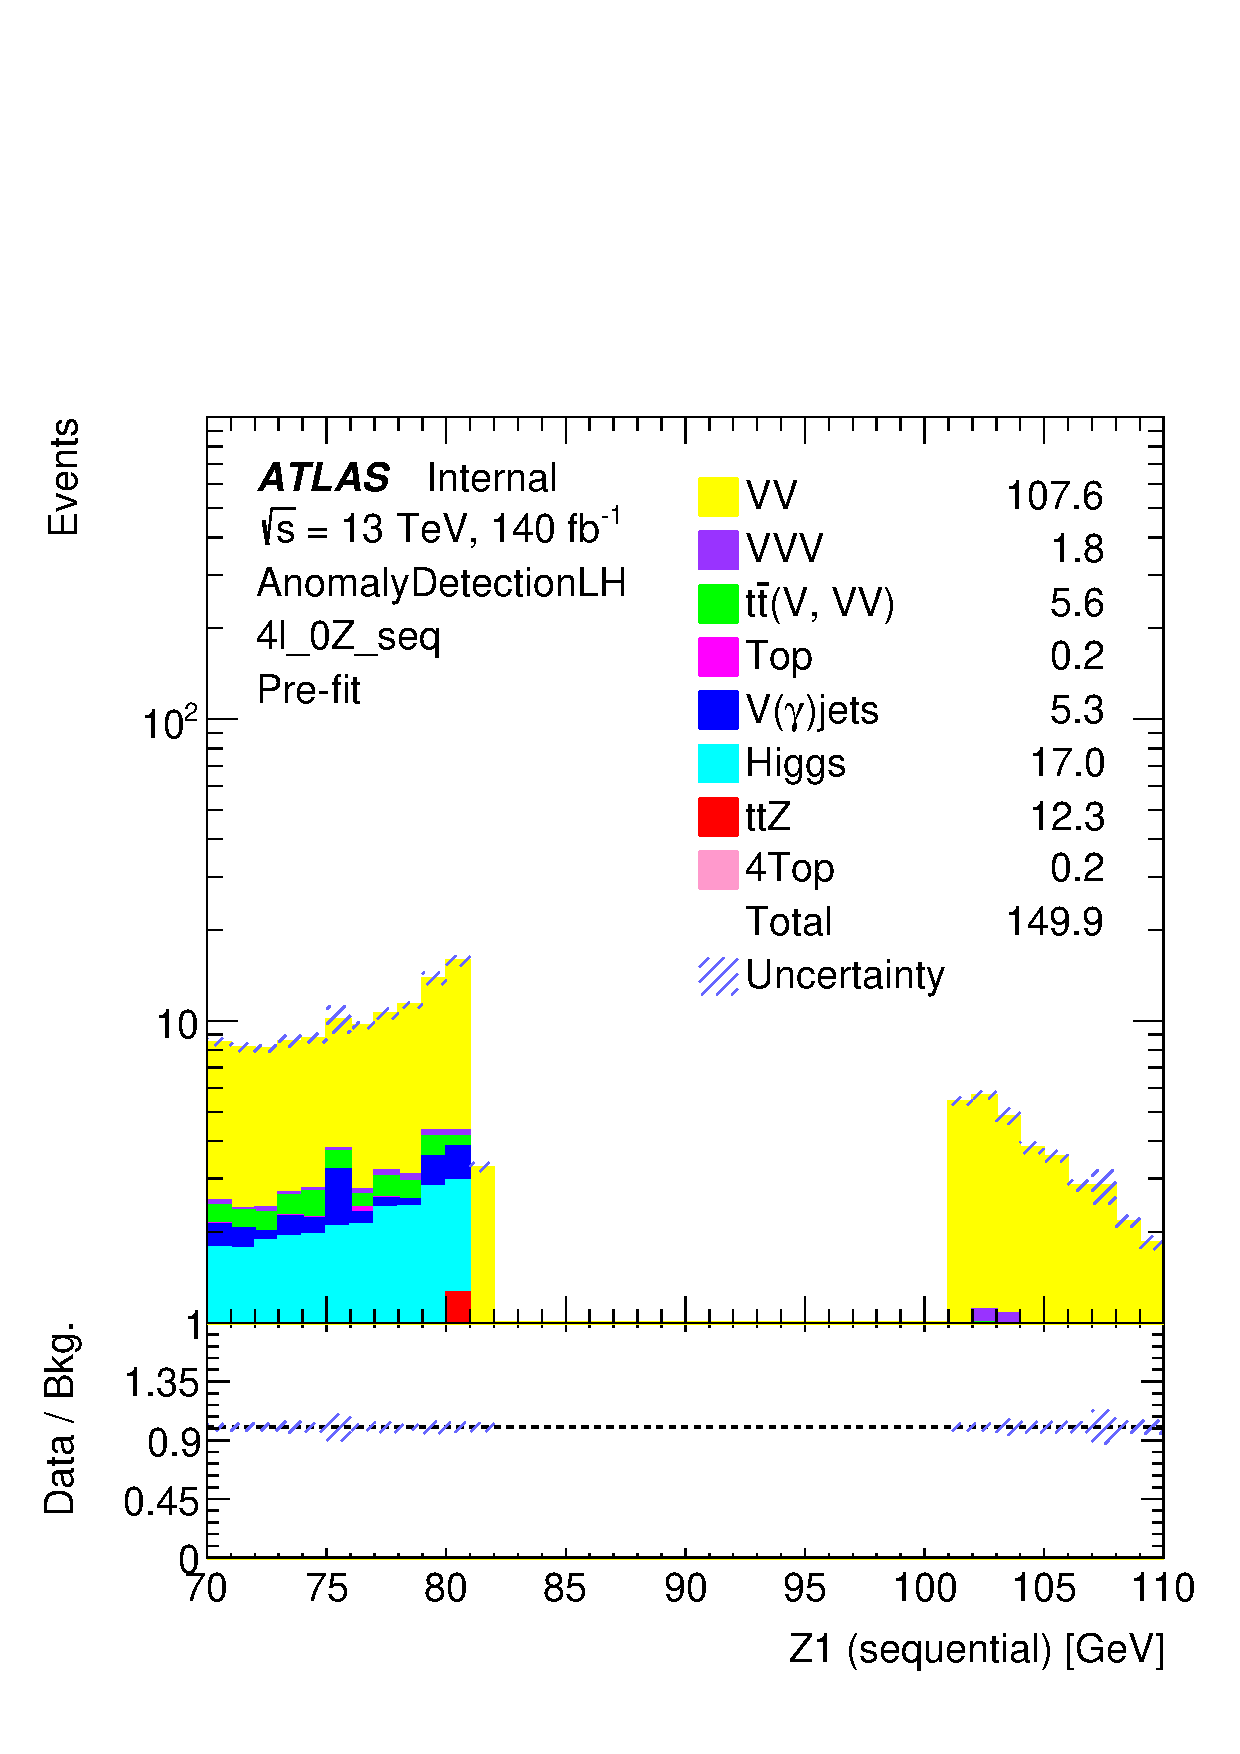
\includegraphics[width=0.24\textwidth]{plots/fourlepLH_run2/Plots/reg_4l_0Z_seq_Z1_mass_seq_1GeV.pdf} &
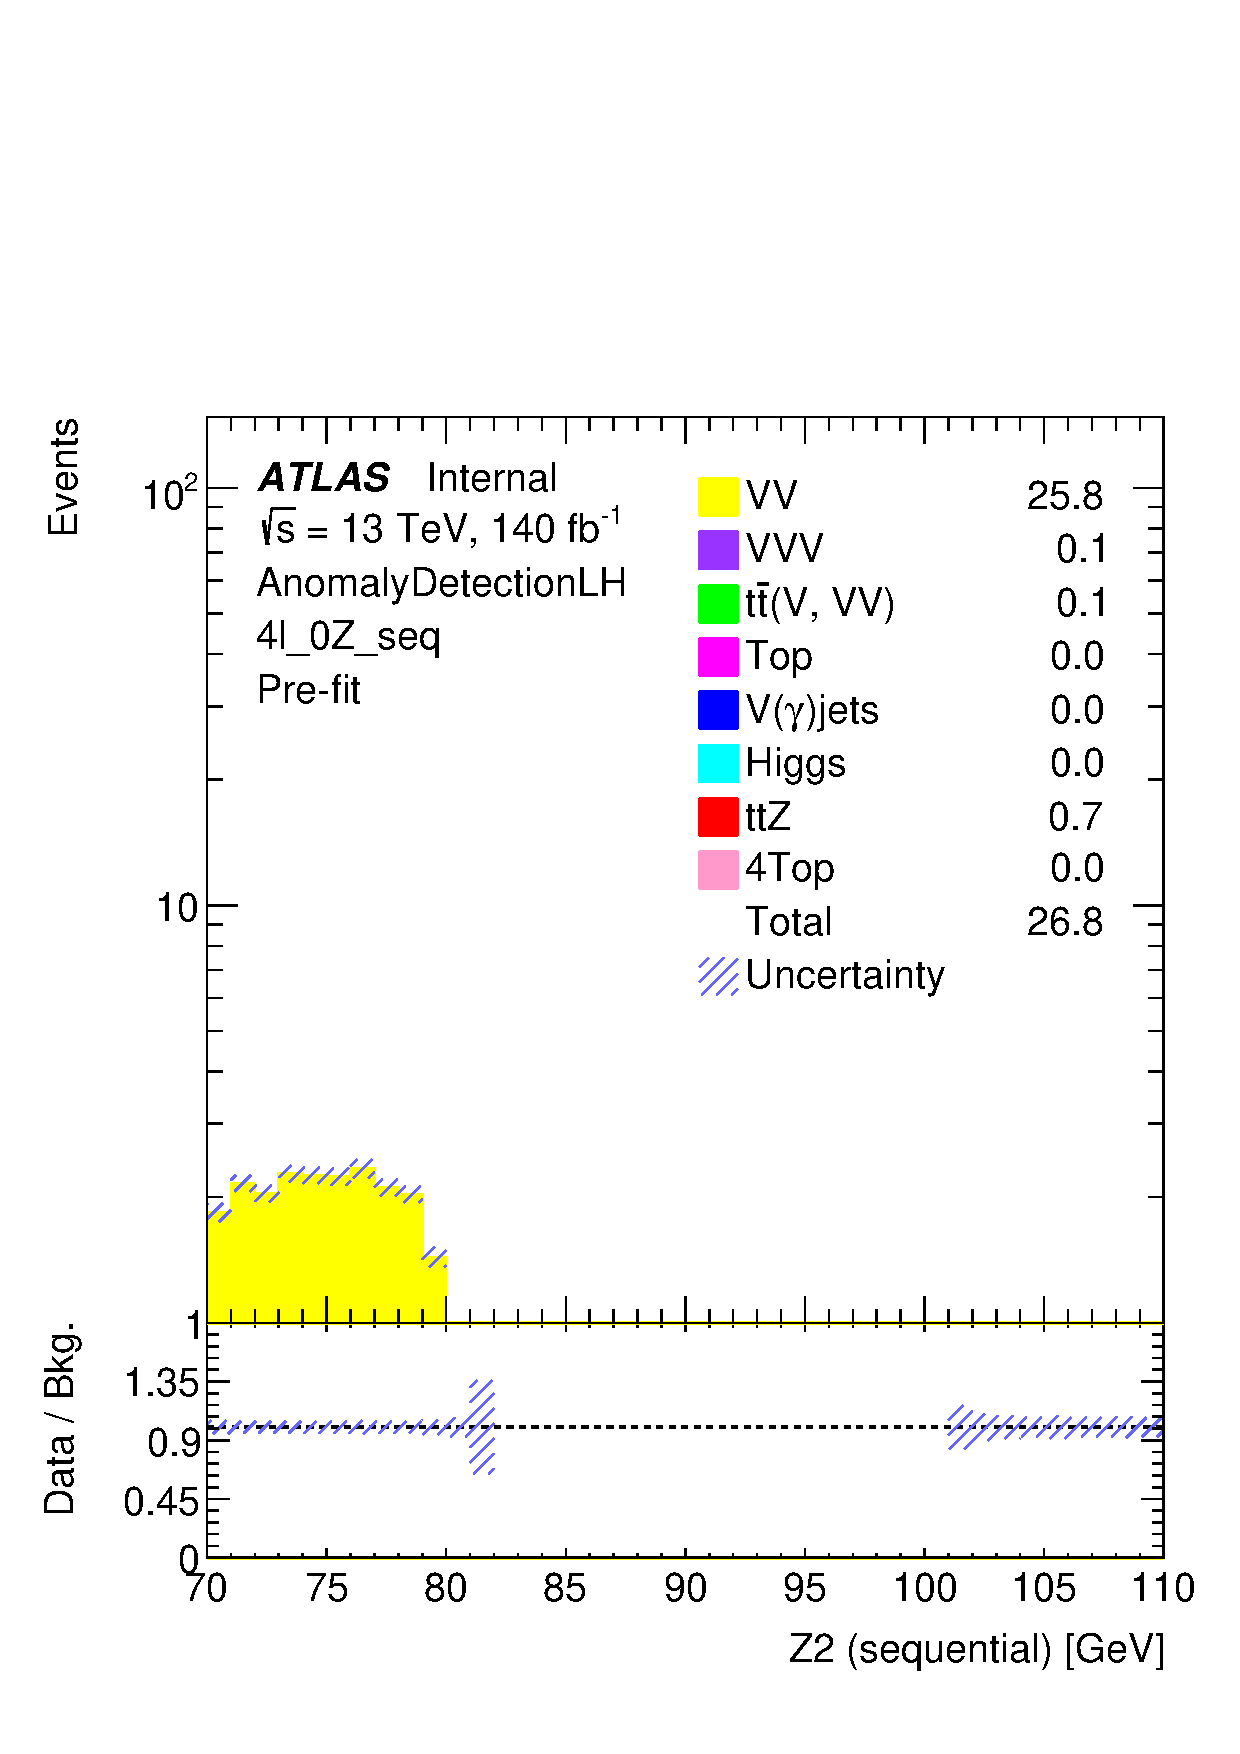
\includegraphics[width=0.24\textwidth]{plots/fourlepLH_run2/Plots/reg_4l_0Z_seq_Z2_mass_seq_1GeV.pdf}  &

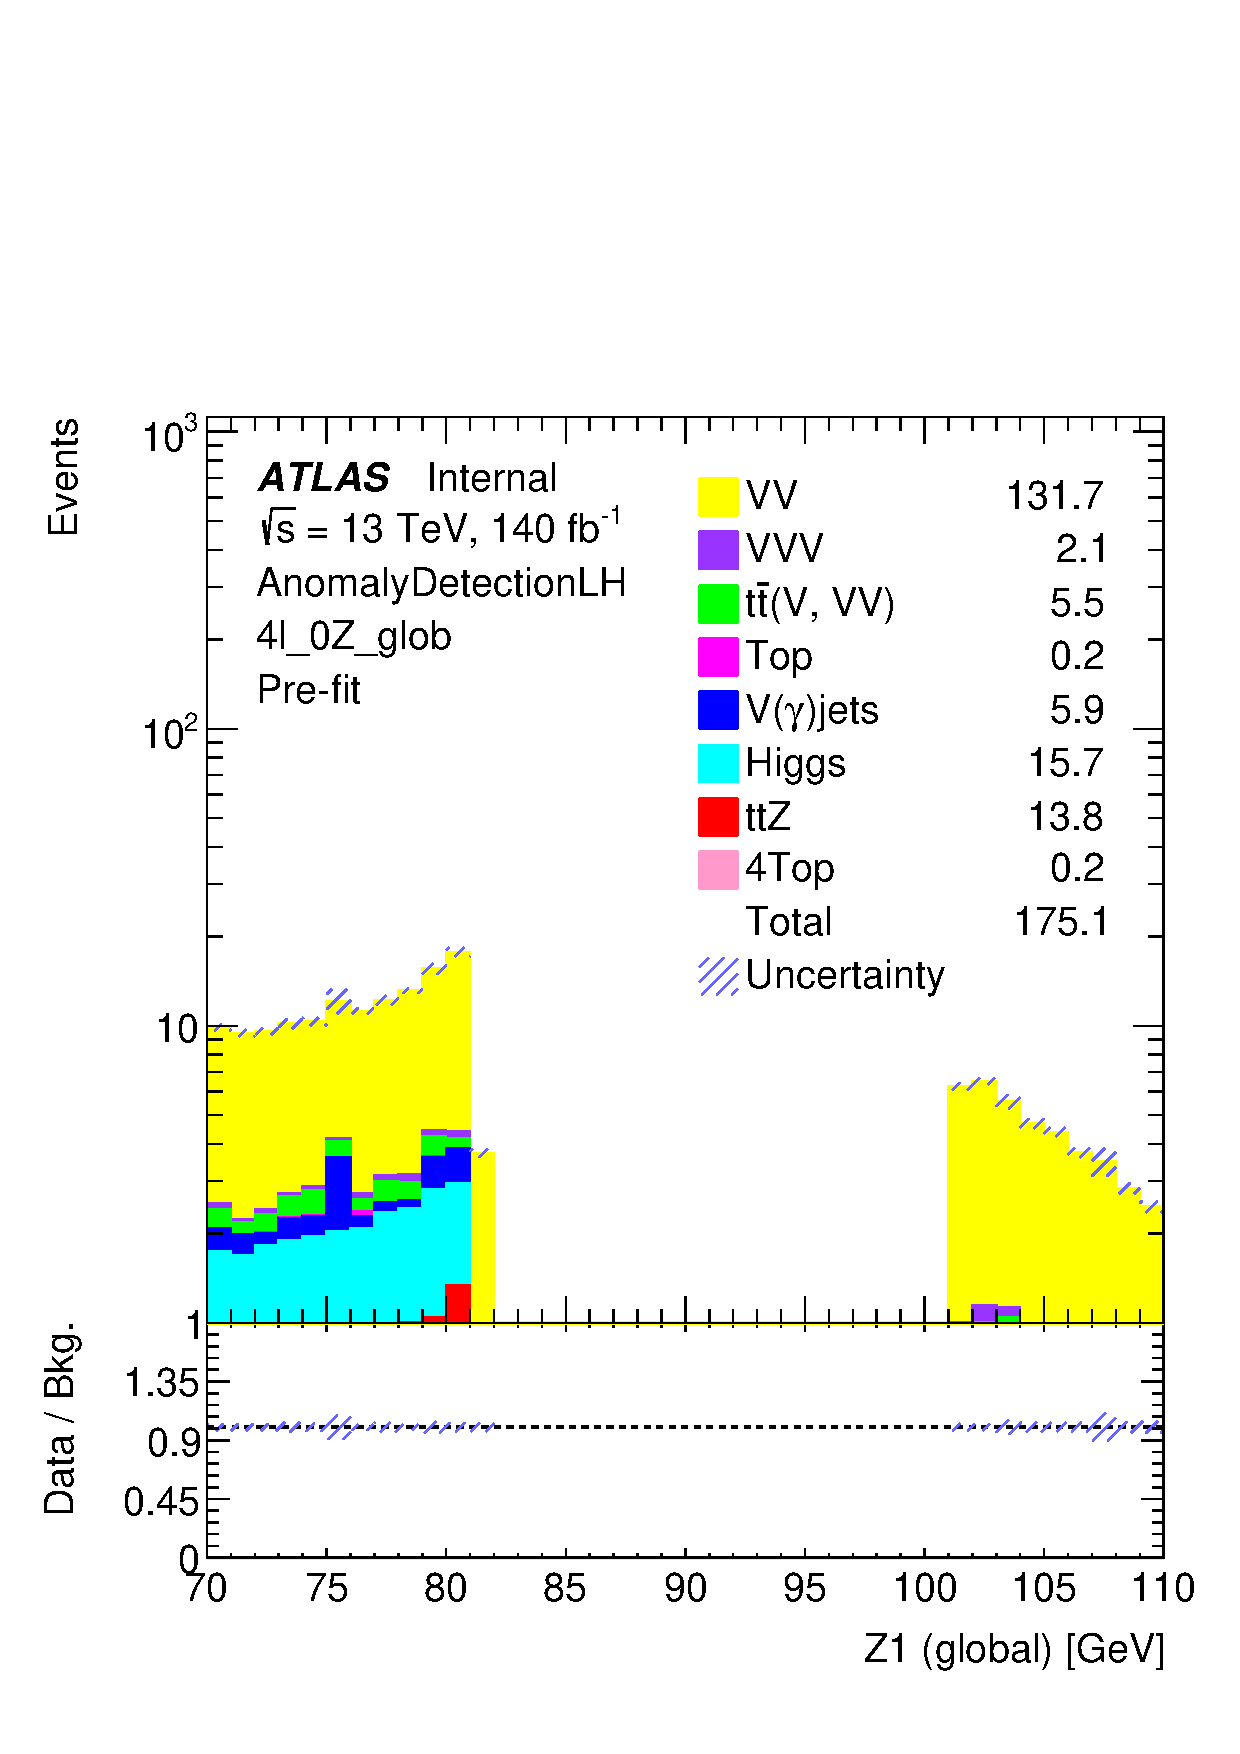
\includegraphics[width=0.24\textwidth]{plots/fourlepLH_run2/Plots/reg_4l_0Z_glob_Z1_mass_glob_1GeV.pdf} &
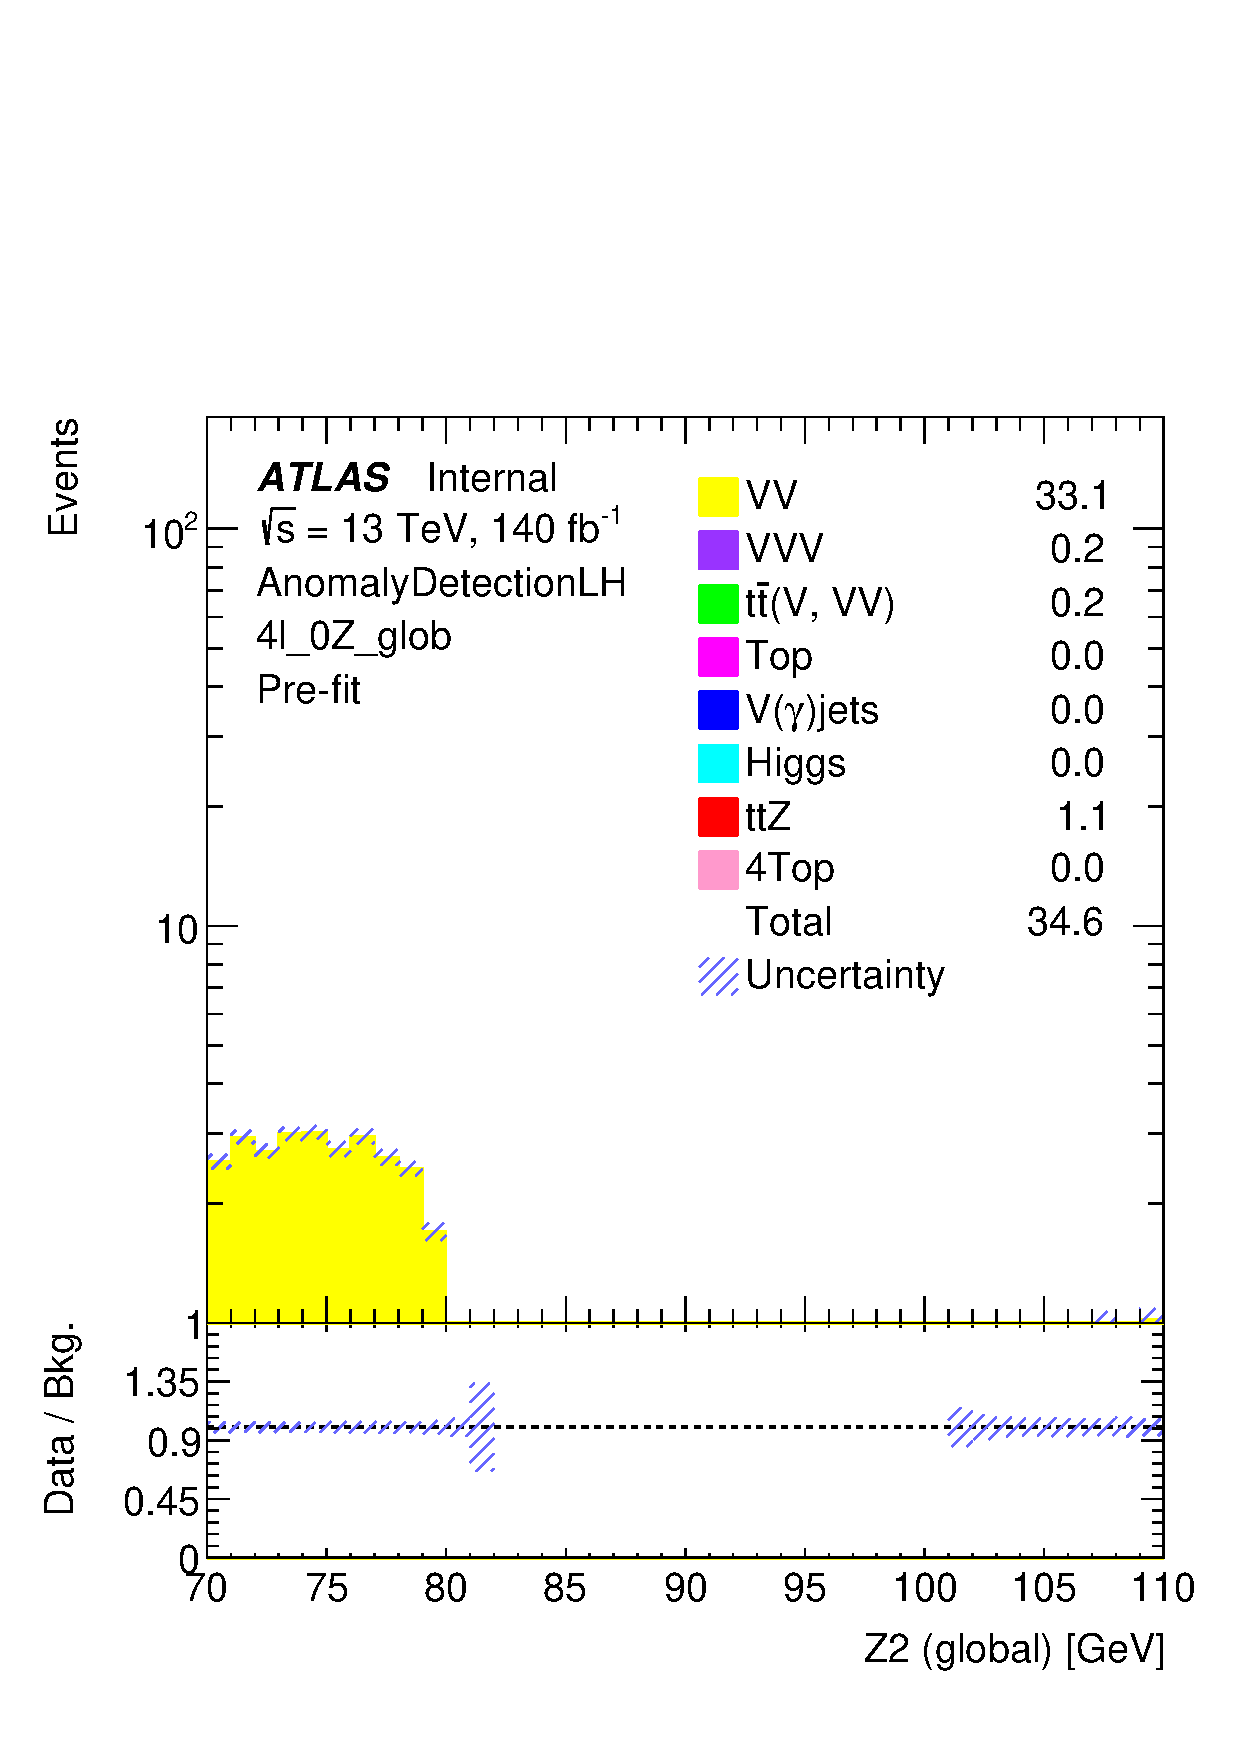
\includegraphics[width=0.24\textwidth]{plots/fourlepLH_run2/Plots/reg_4l_0Z_glob_Z2_mass_glob_1GeV.pdf}\\

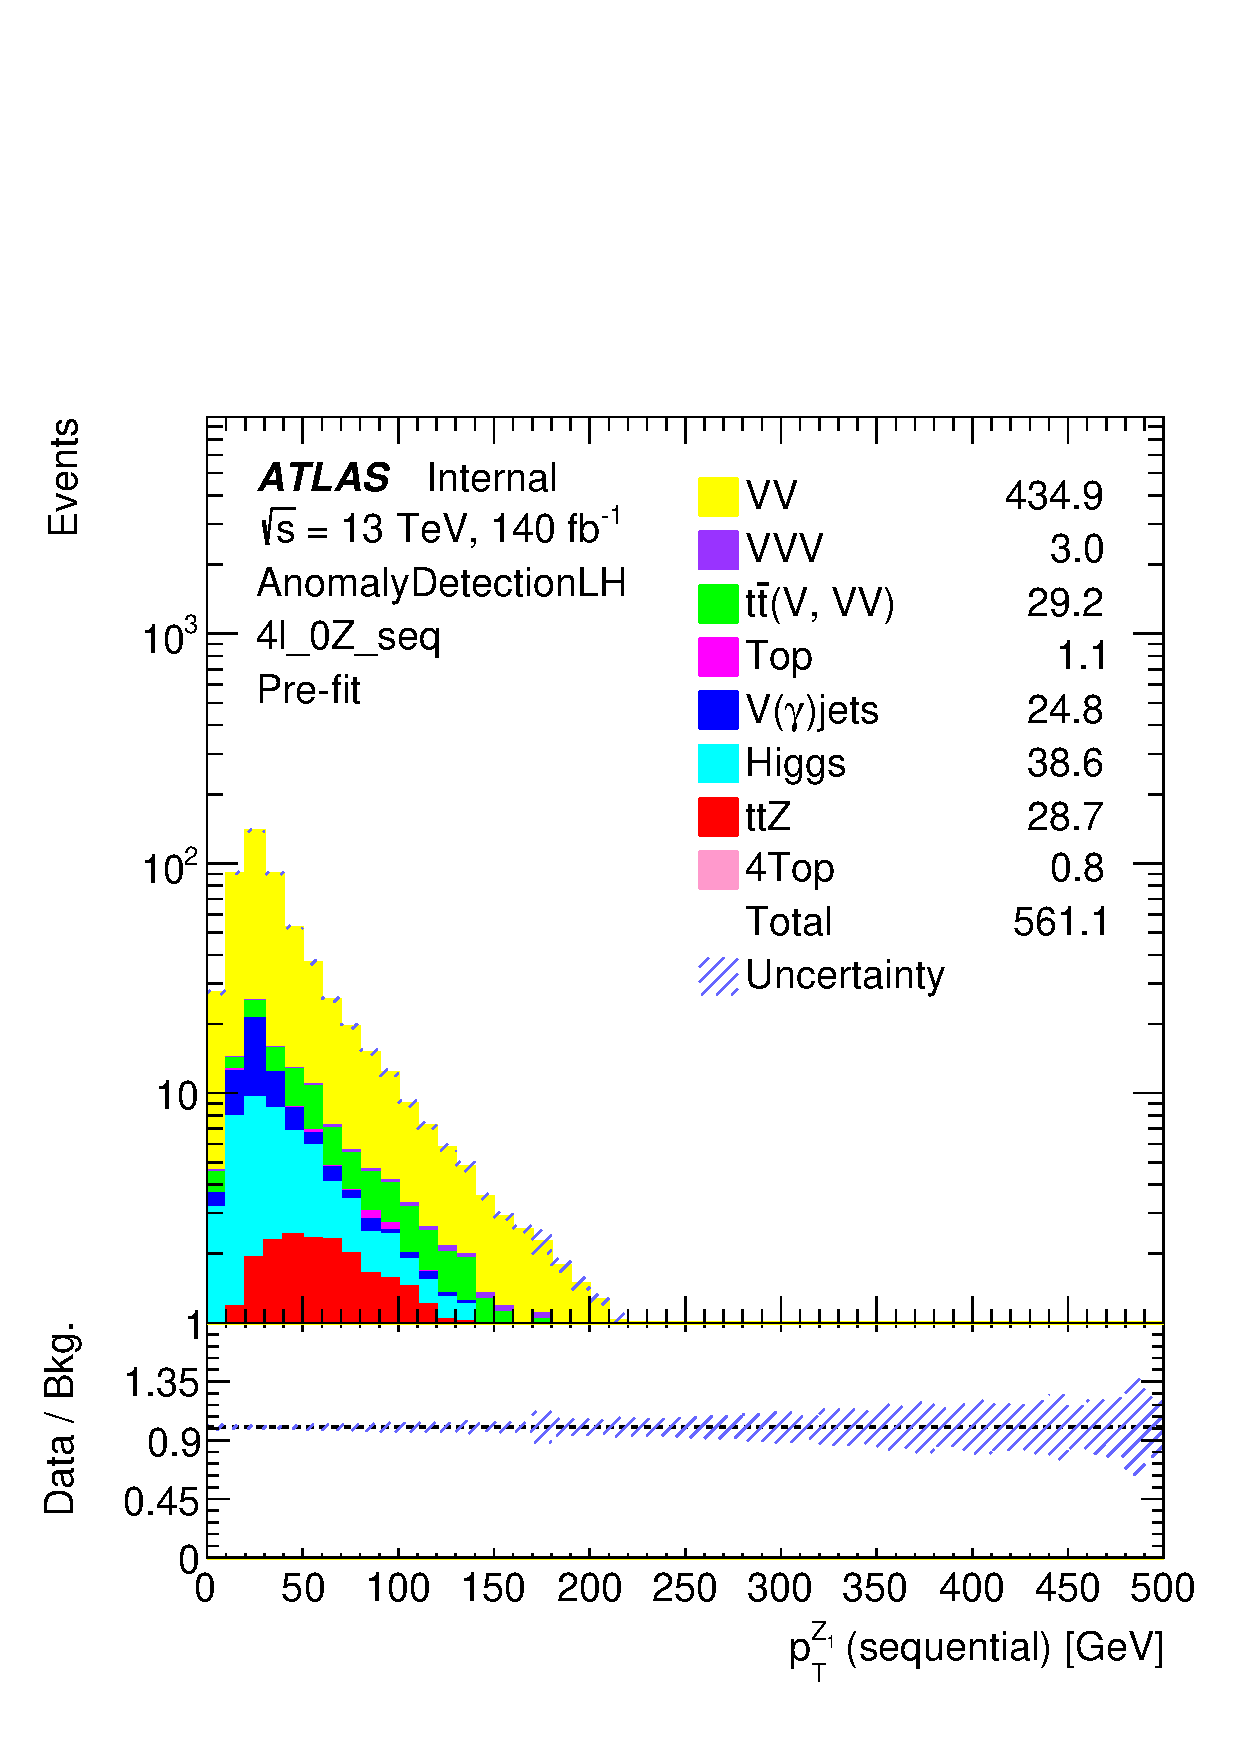
\includegraphics[width=0.24\textwidth]{plots/fourlepLH_run2/Plots/reg_4l_0Z_seq_Z1_pt_seq.pdf} &
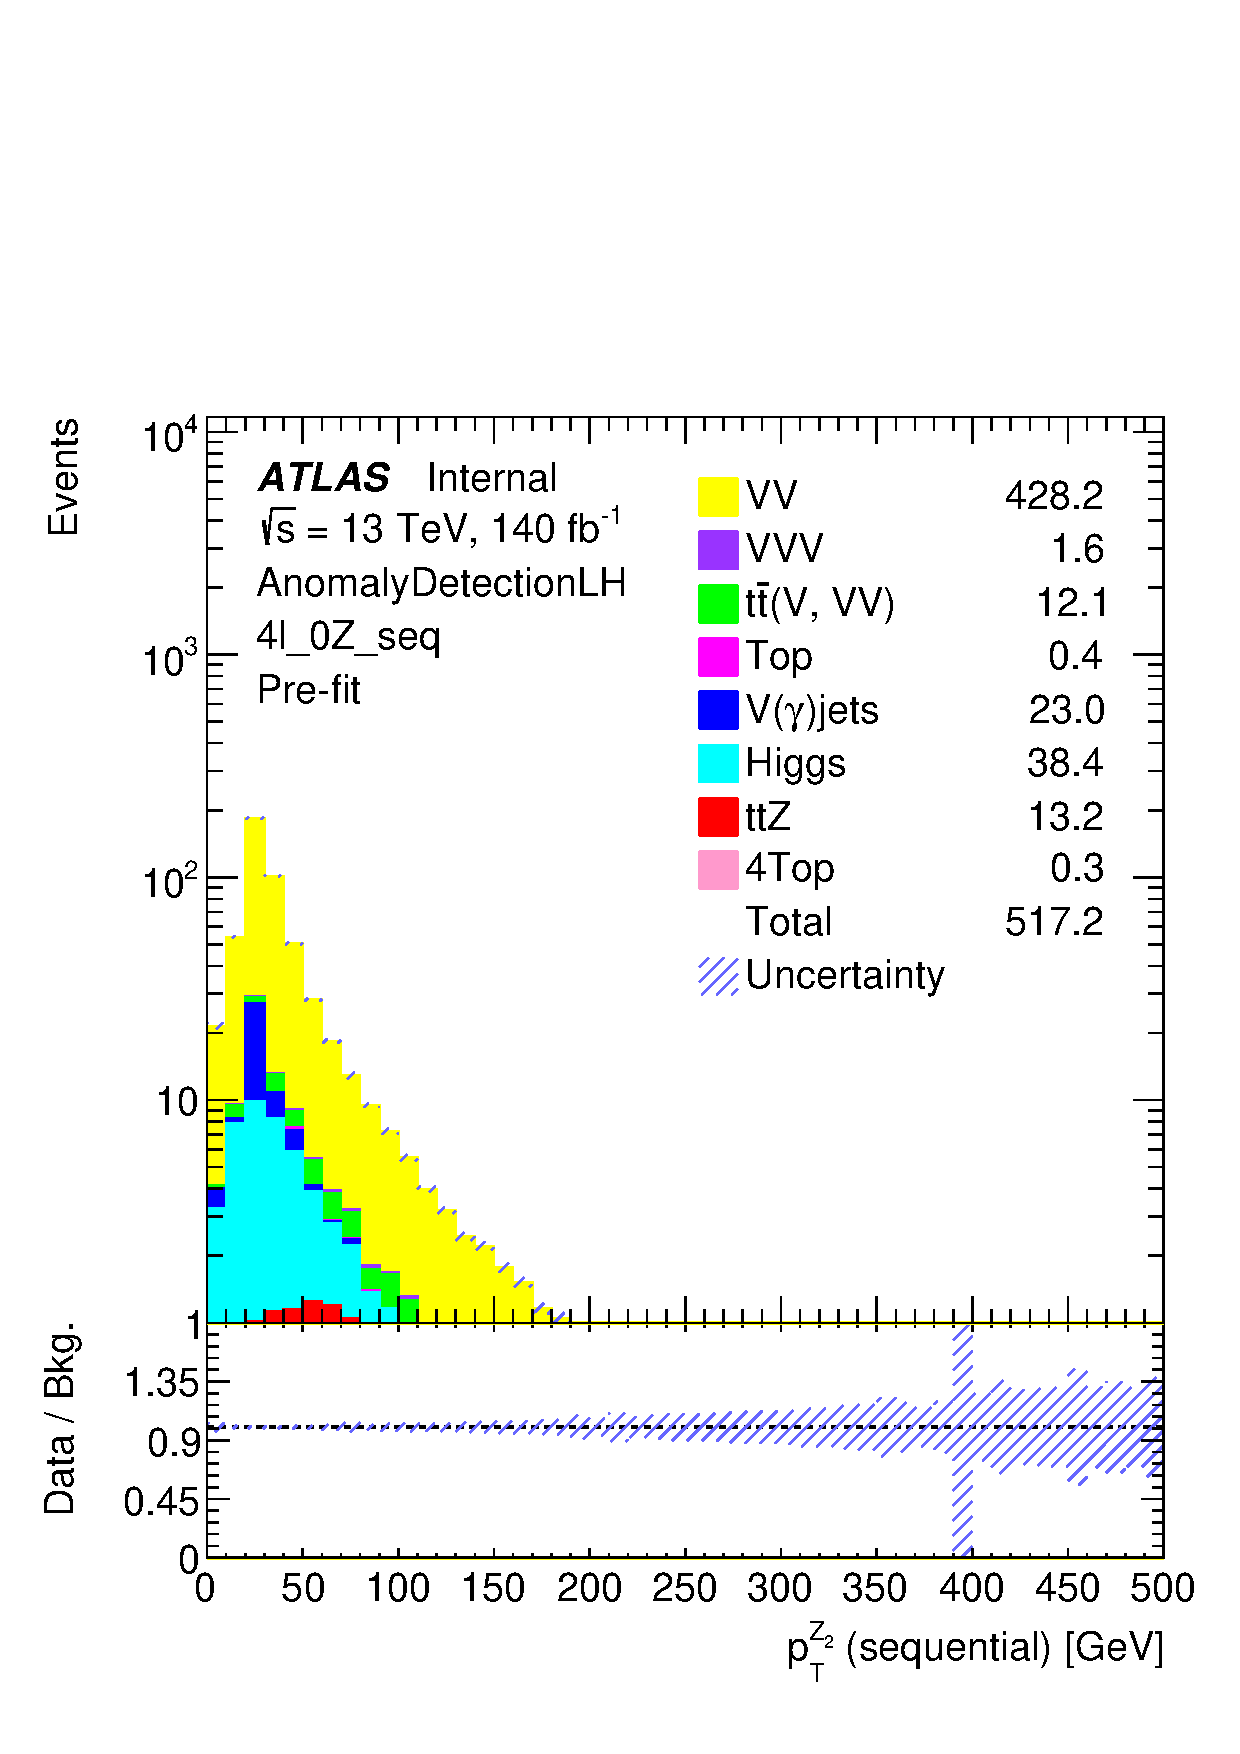
\includegraphics[width=0.24\textwidth]{plots/fourlepLH_run2/Plots/reg_4l_0Z_seq_Z2_pt_seq.pdf}  &

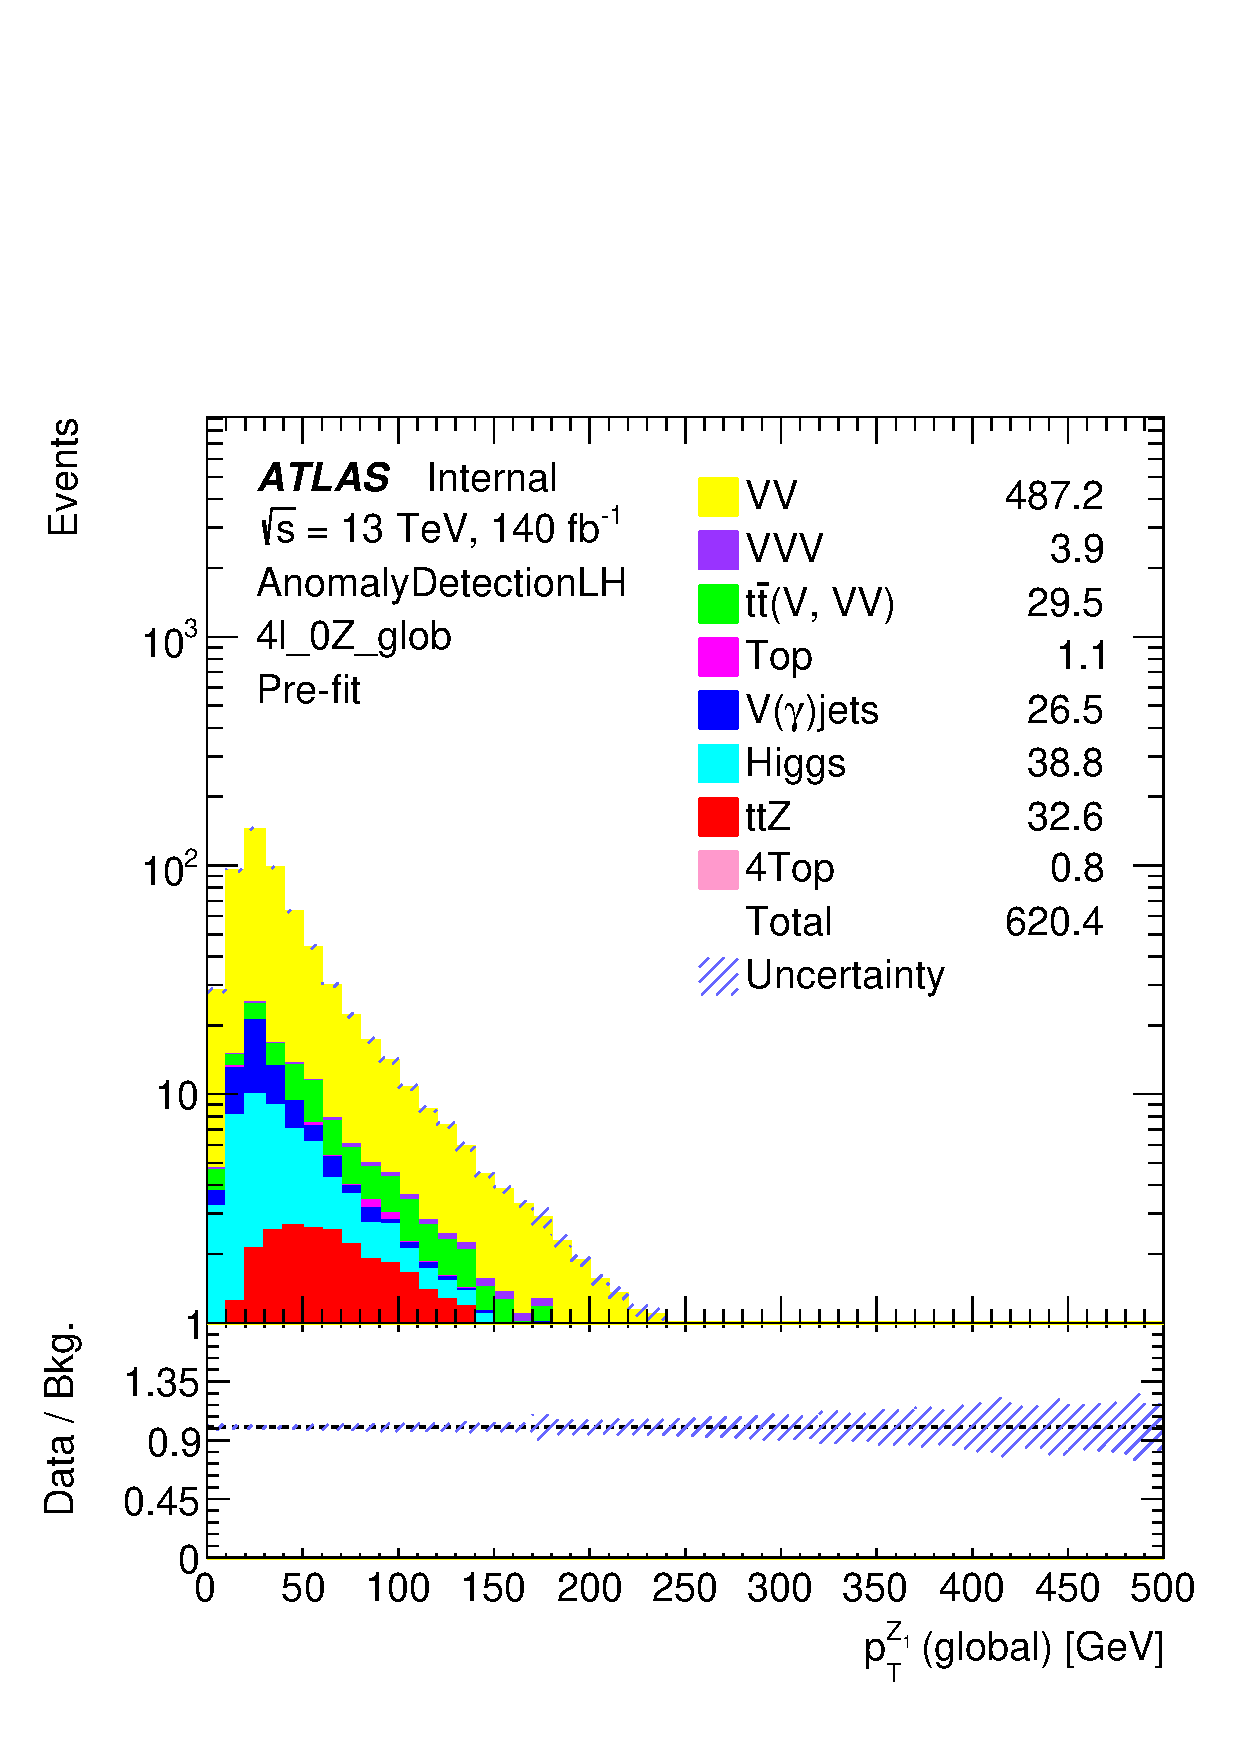
\includegraphics[width=0.24\textwidth]{plots/fourlepLH_run2/Plots/reg_4l_0Z_glob_Z1_pt_glob.pdf} &
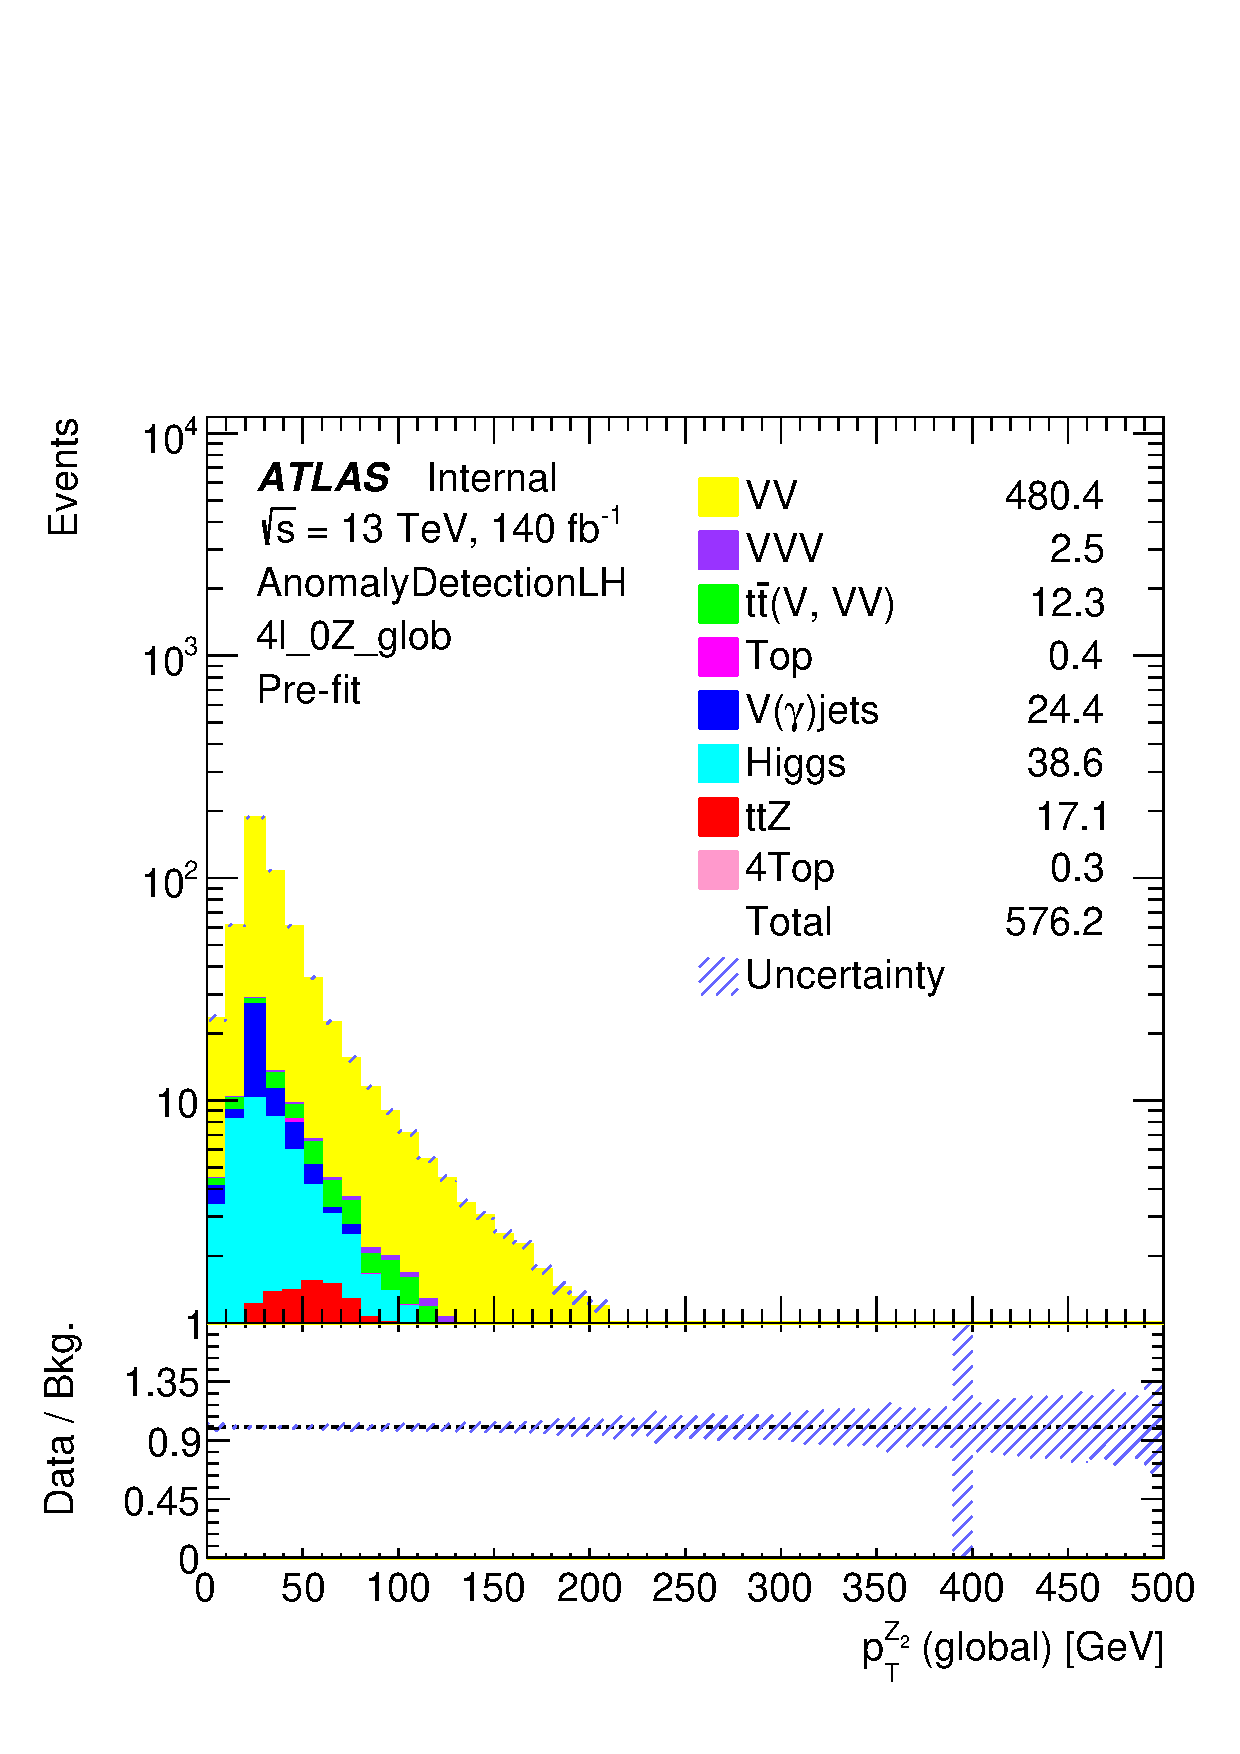
\includegraphics[width=0.24\textwidth]{plots/fourlepLH_run2/Plots/reg_4l_0Z_glob_Z2_pt_glob.pdf}
\end{tabular}
\end{frame}

\begin{frame}{\texttt{Results: 4l\_0Z}}
\begin{tabular}{cccccc}
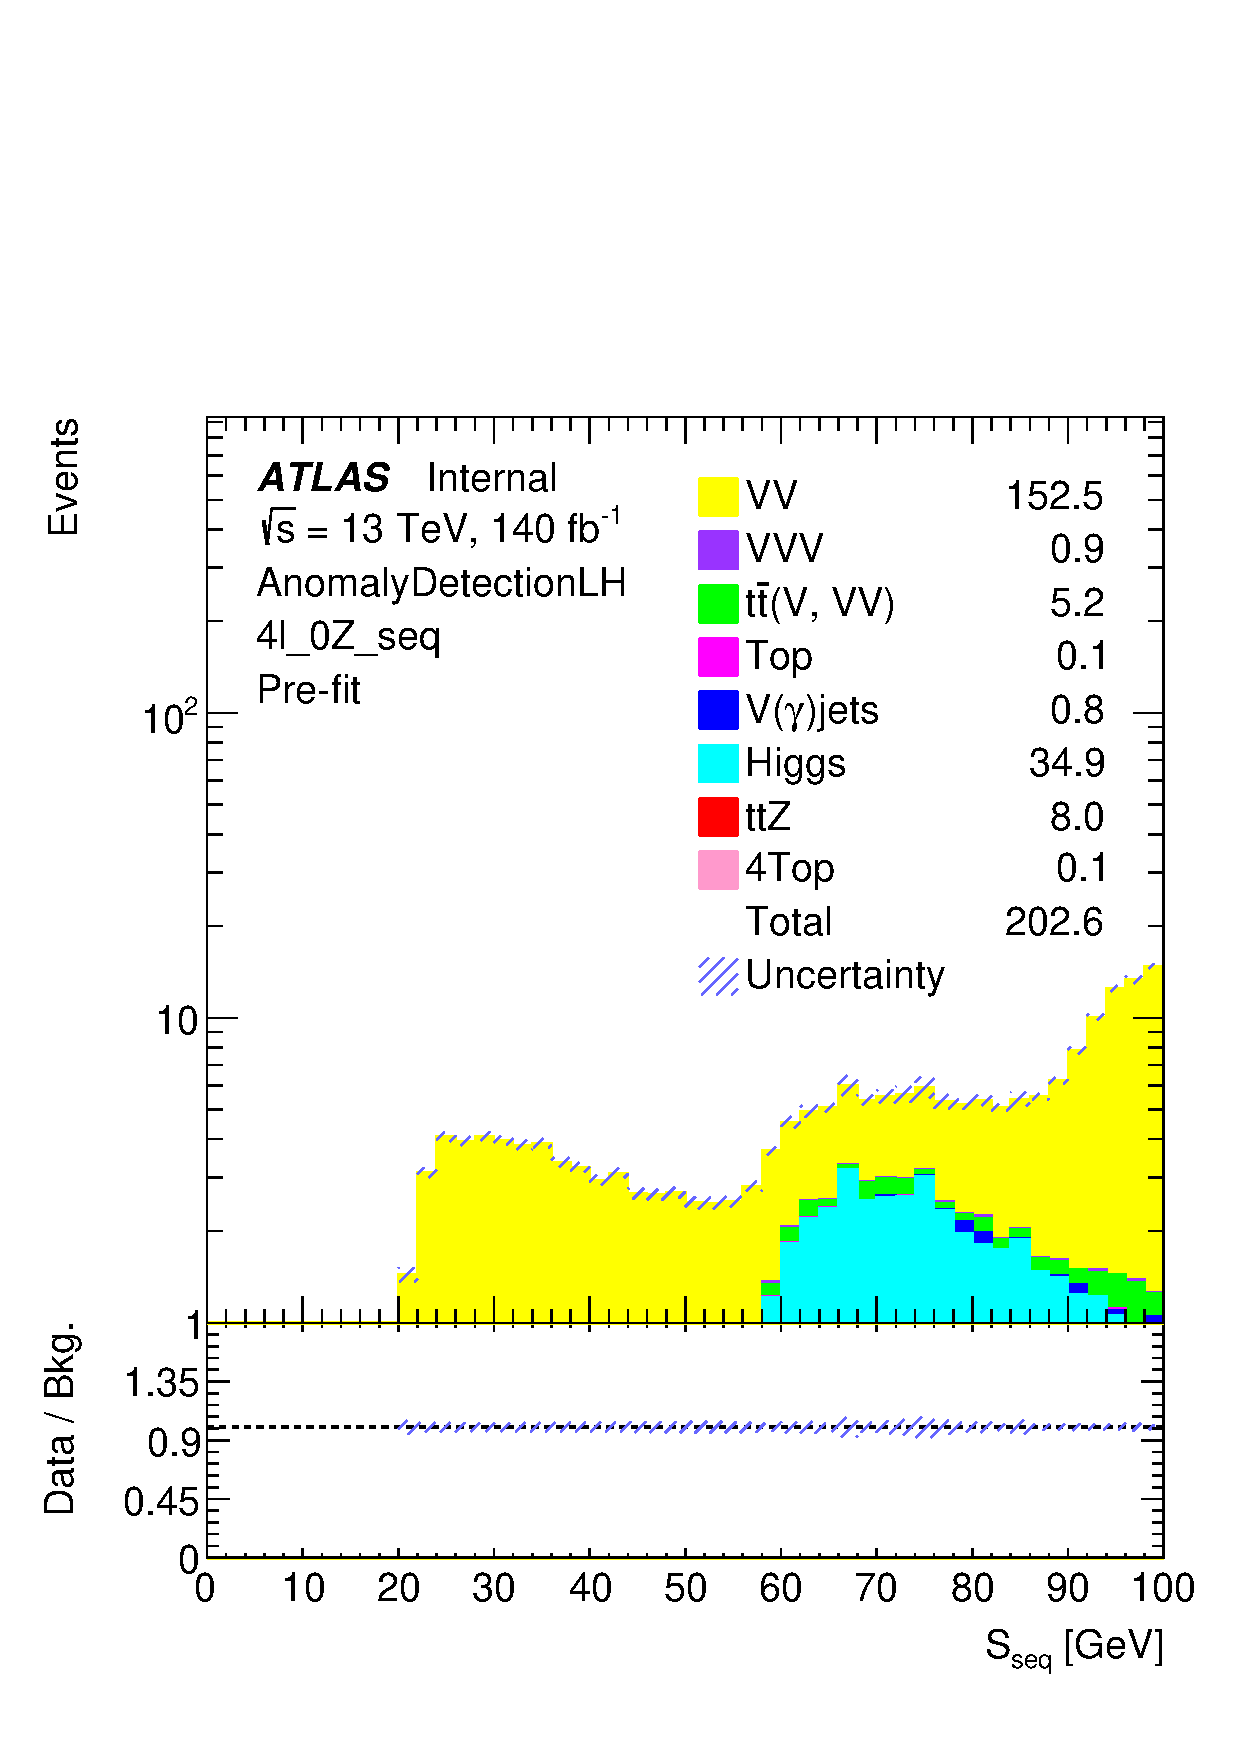
\includegraphics[width=0.24\textwidth]{plots/fourlepLH_run2/Plots/reg_4l_0Z_seq_Zscore_seq.pdf} & 
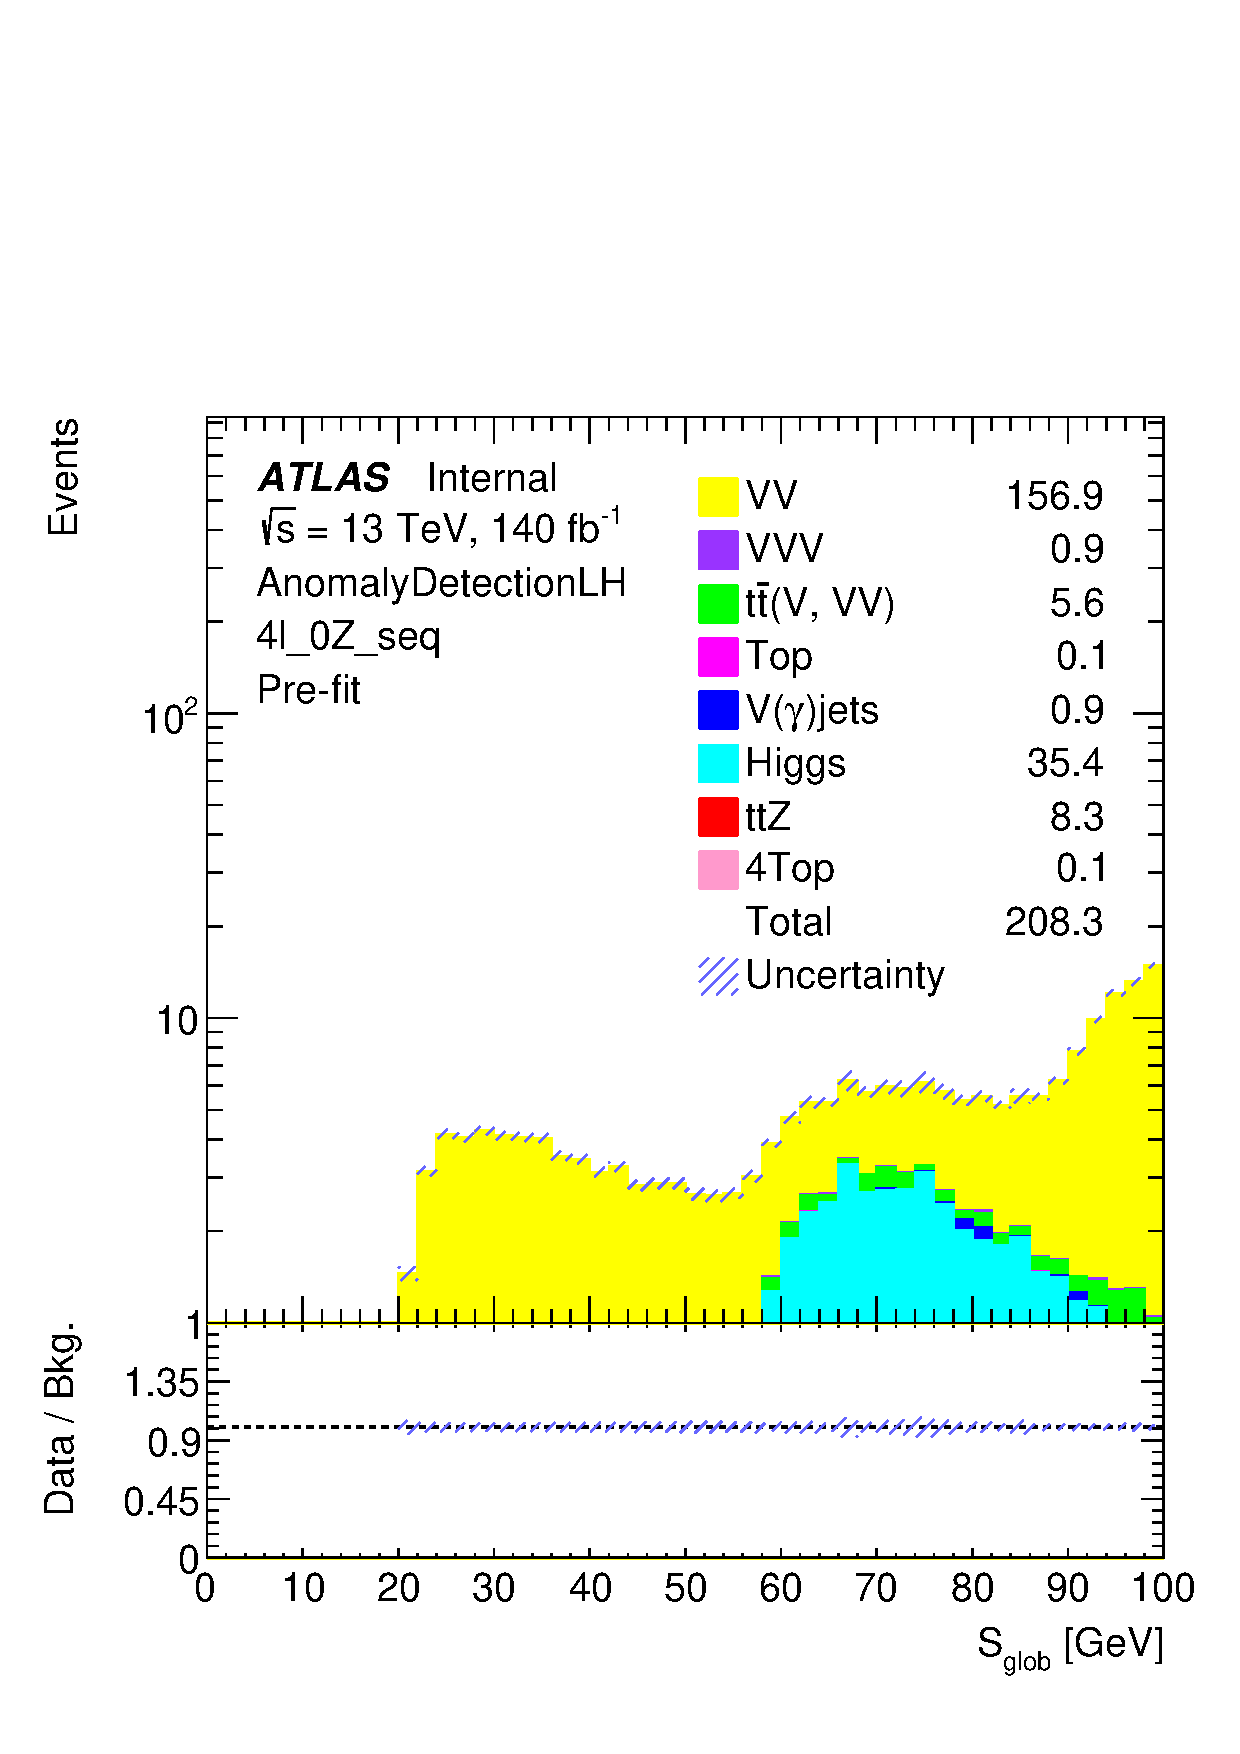
\includegraphics[width=0.24\textwidth]{plots/fourlepLH_run2/Plots/reg_4l_0Z_seq_Zscore_glob.pdf}&
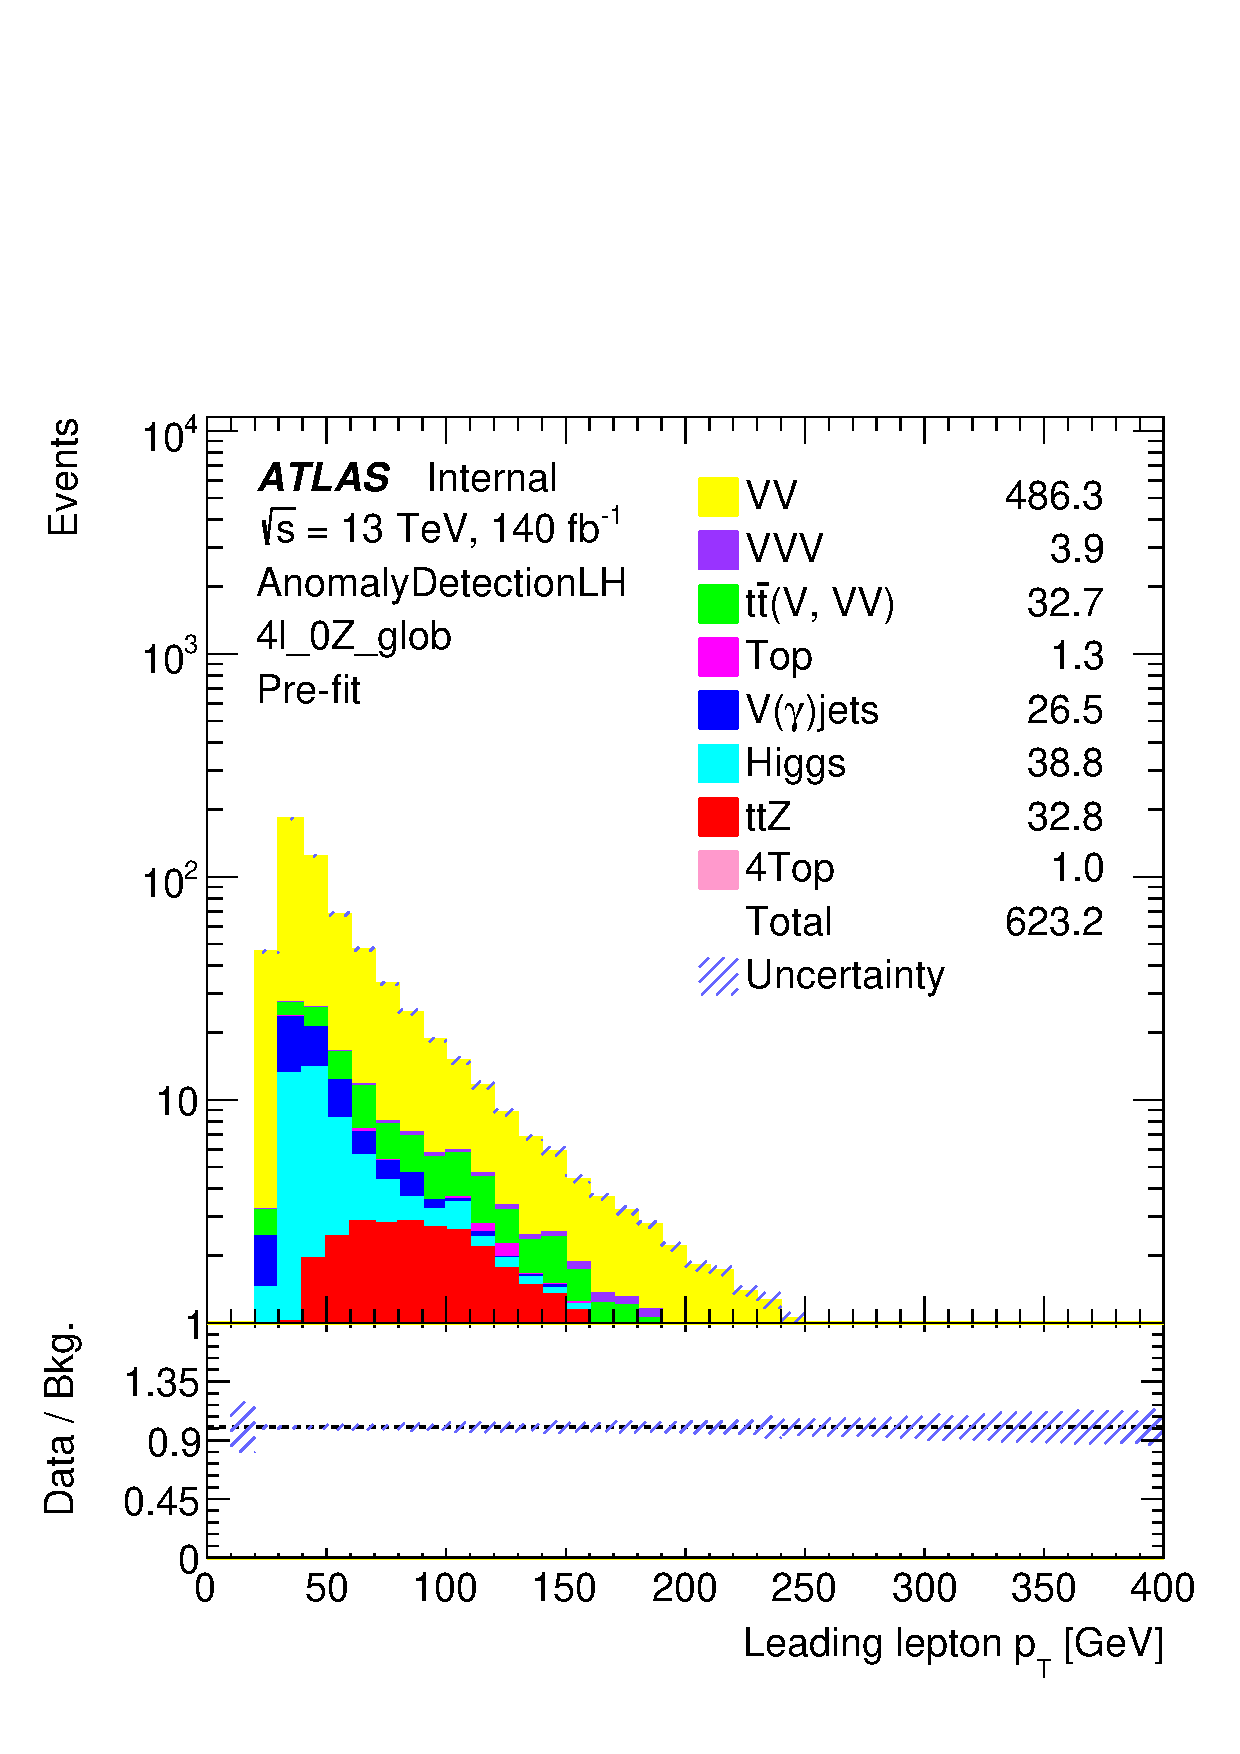
\includegraphics[width=0.24\textwidth]{plots/fourlepLH_run2/Plots/reg_4l_0Z_seq_deltaZscore.pdf}\\

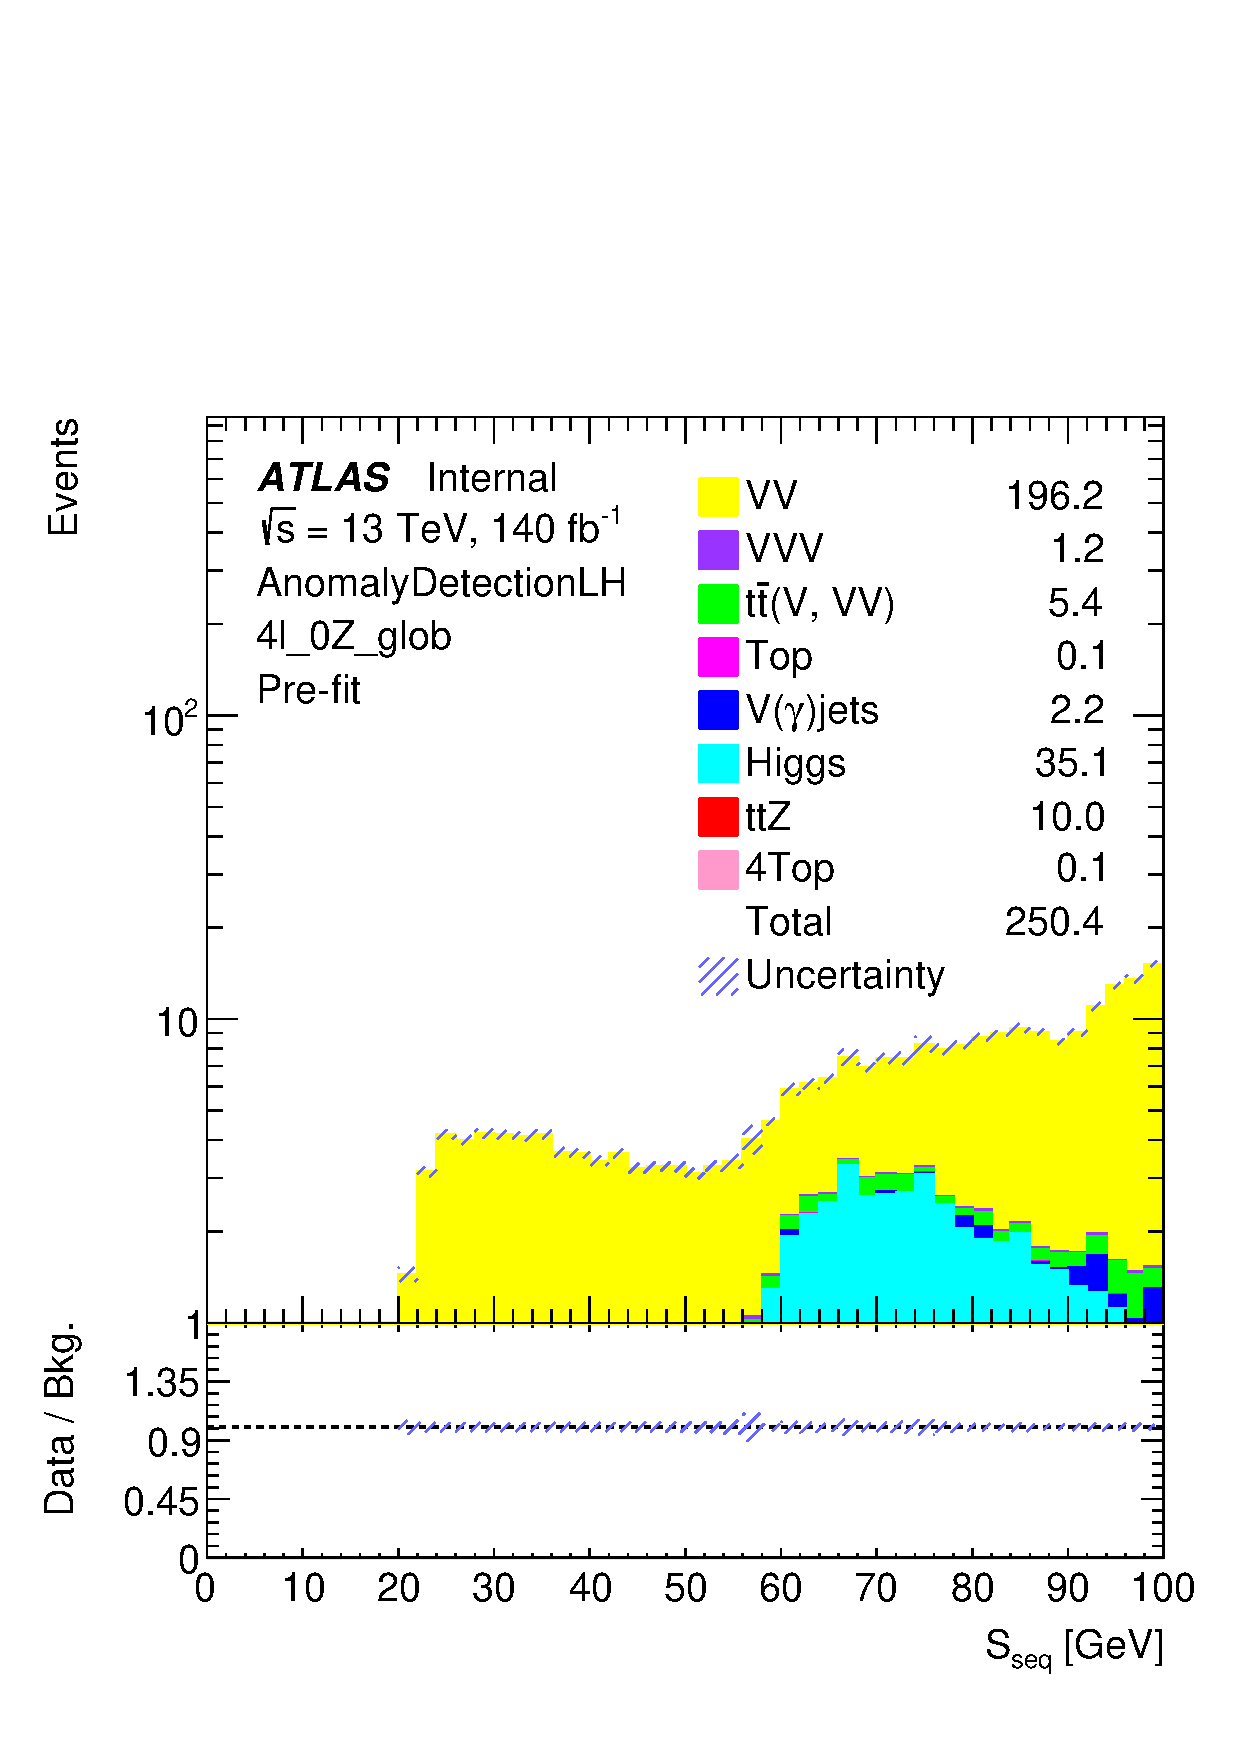
\includegraphics[width=0.24\textwidth]{plots/fourlepLH_run2/Plots/reg_4l_0Z_glob_Zscore_seq.pdf} & 
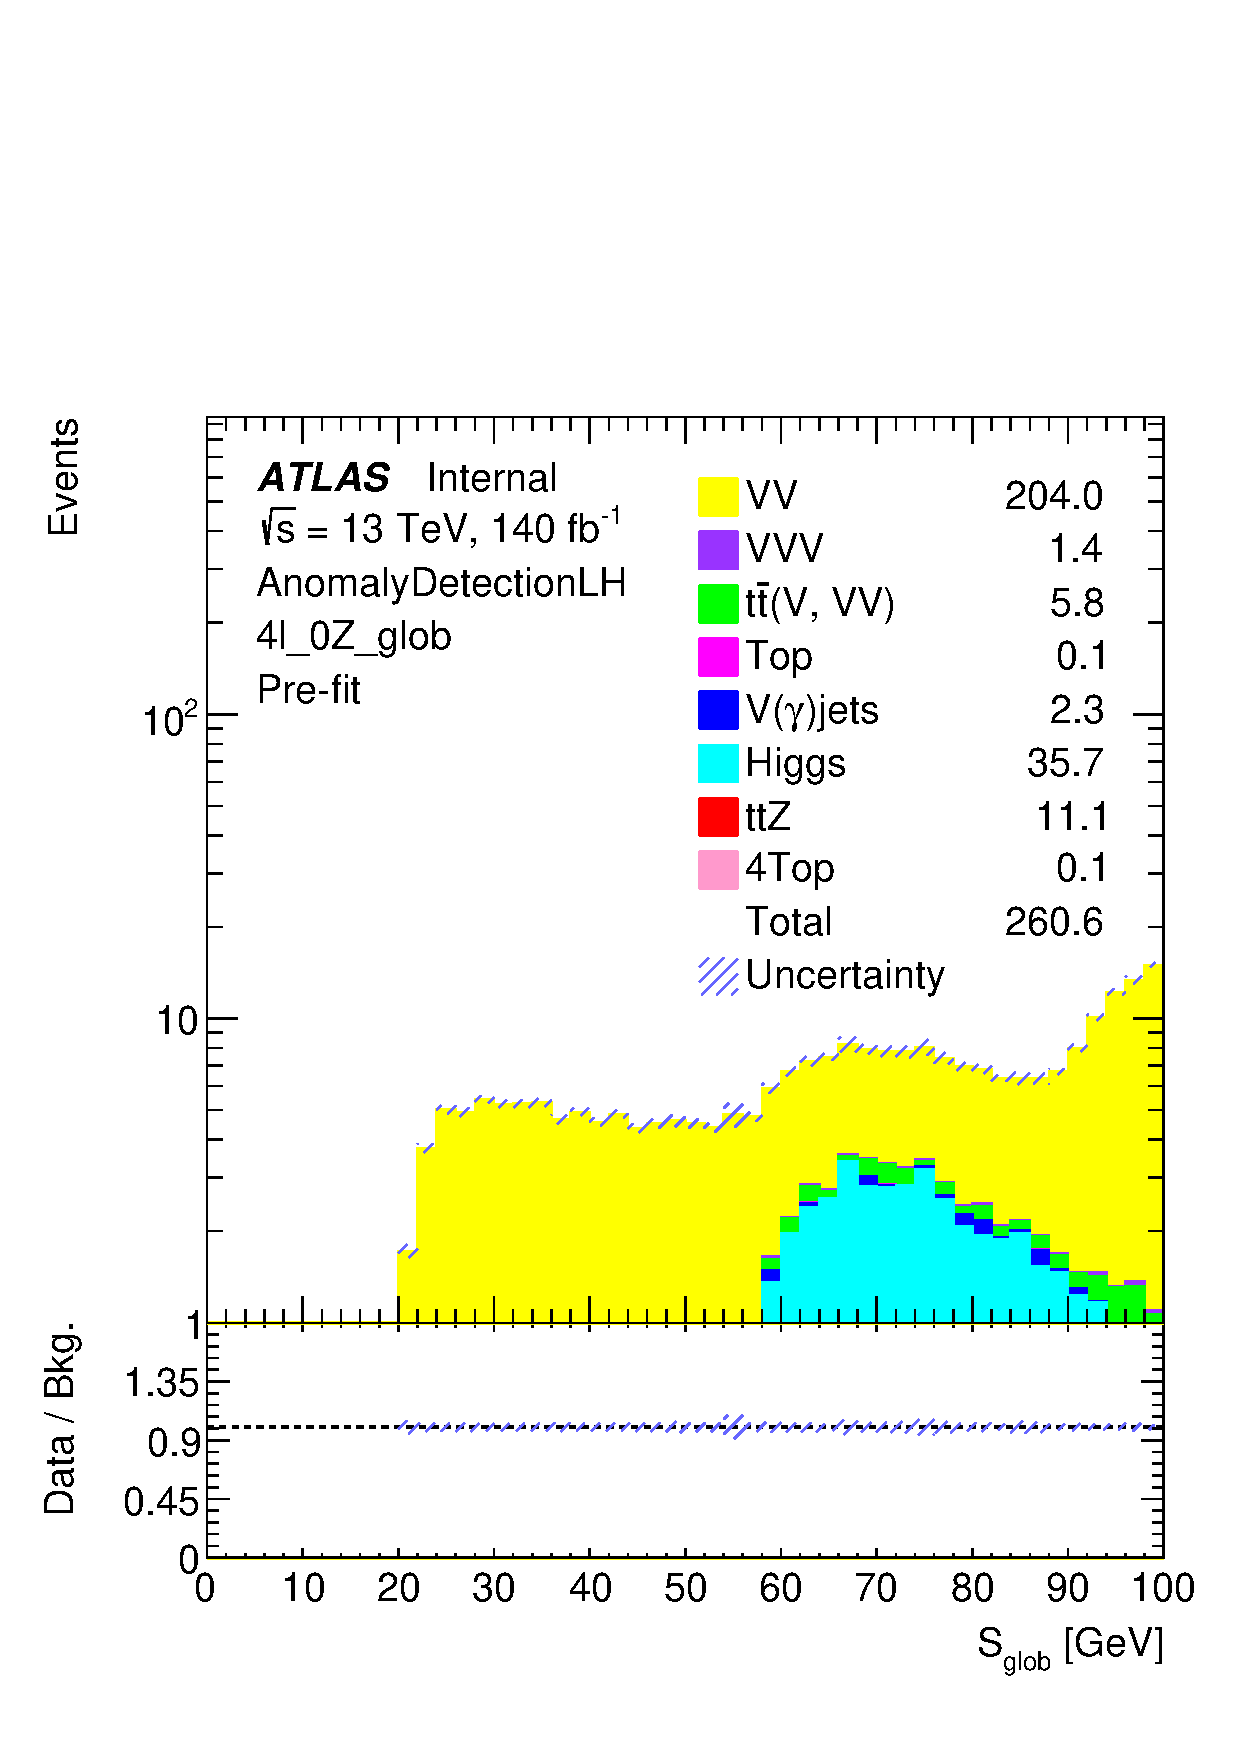
\includegraphics[width=0.24\textwidth]{plots/fourlepLH_run2/Plots/reg_4l_0Z_glob_Zscore_glob.pdf}&
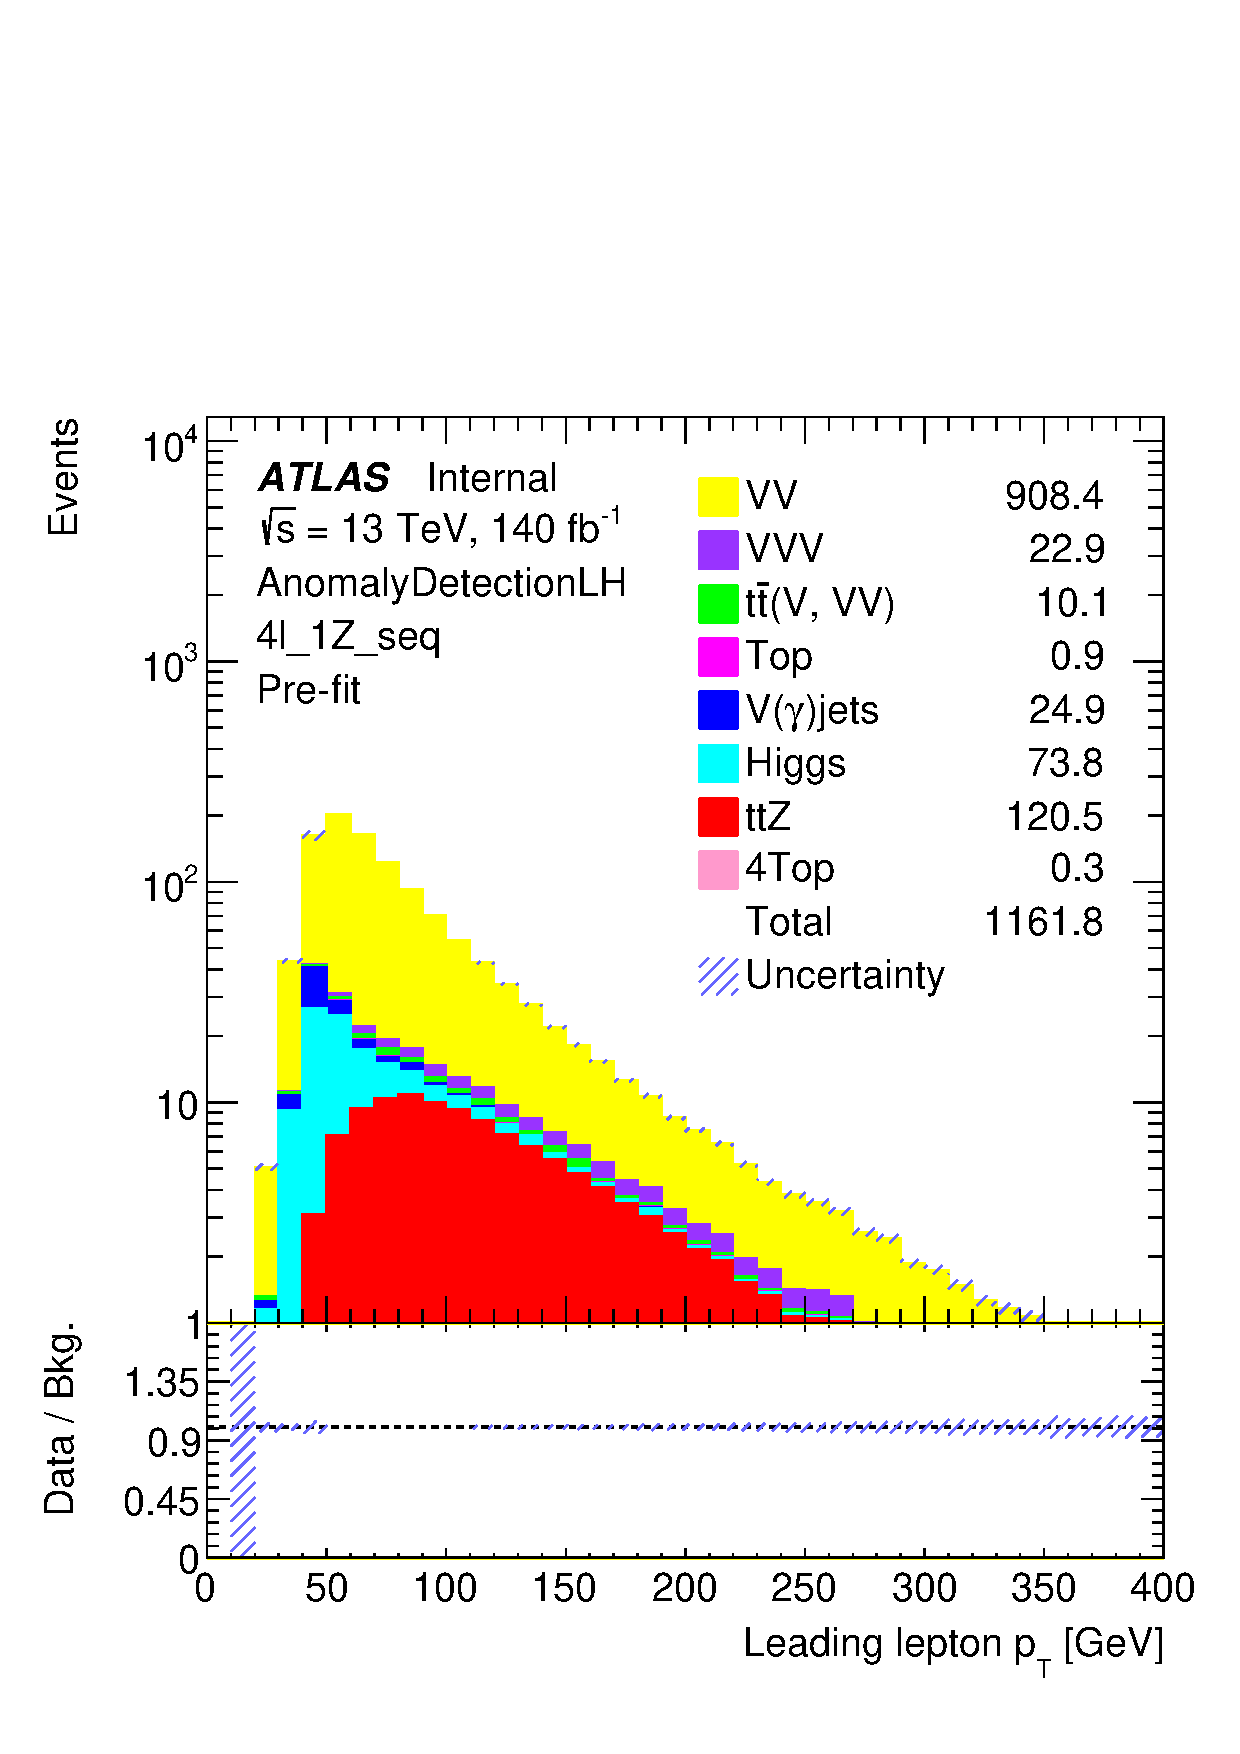
\includegraphics[width=0.24\textwidth]{plots/fourlepLH_run2/Plots/reg_4l_0Z_glob_deltaZscore.pdf}
\end{tabular}
\end{frame}


\begin{frame}{\texttt{Results: 4l\_0Z}}
\begin{tabular}{cccccc}

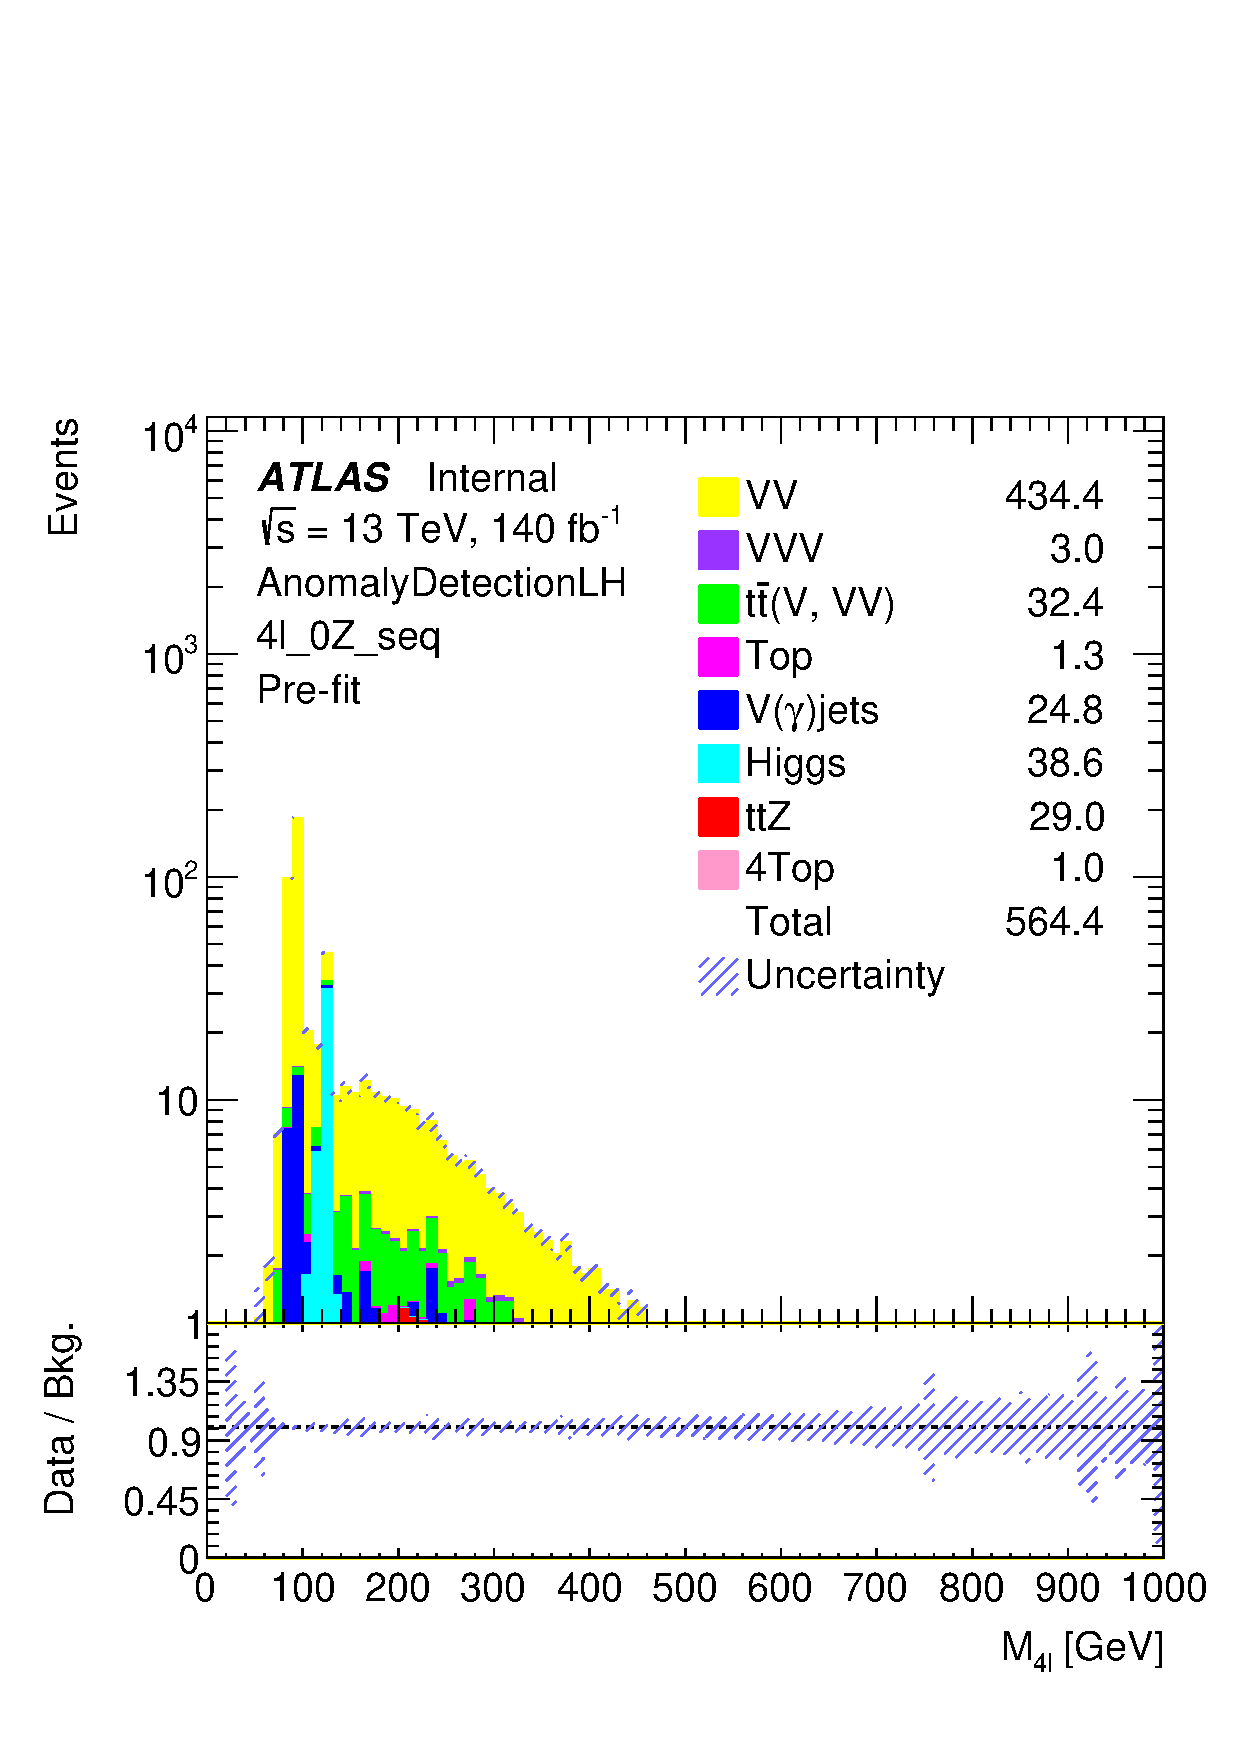
\includegraphics[width=0.24\textwidth]{plots/fourlepLH_run2/Plots/reg_4l_0Z_seq_m4l.pdf} &
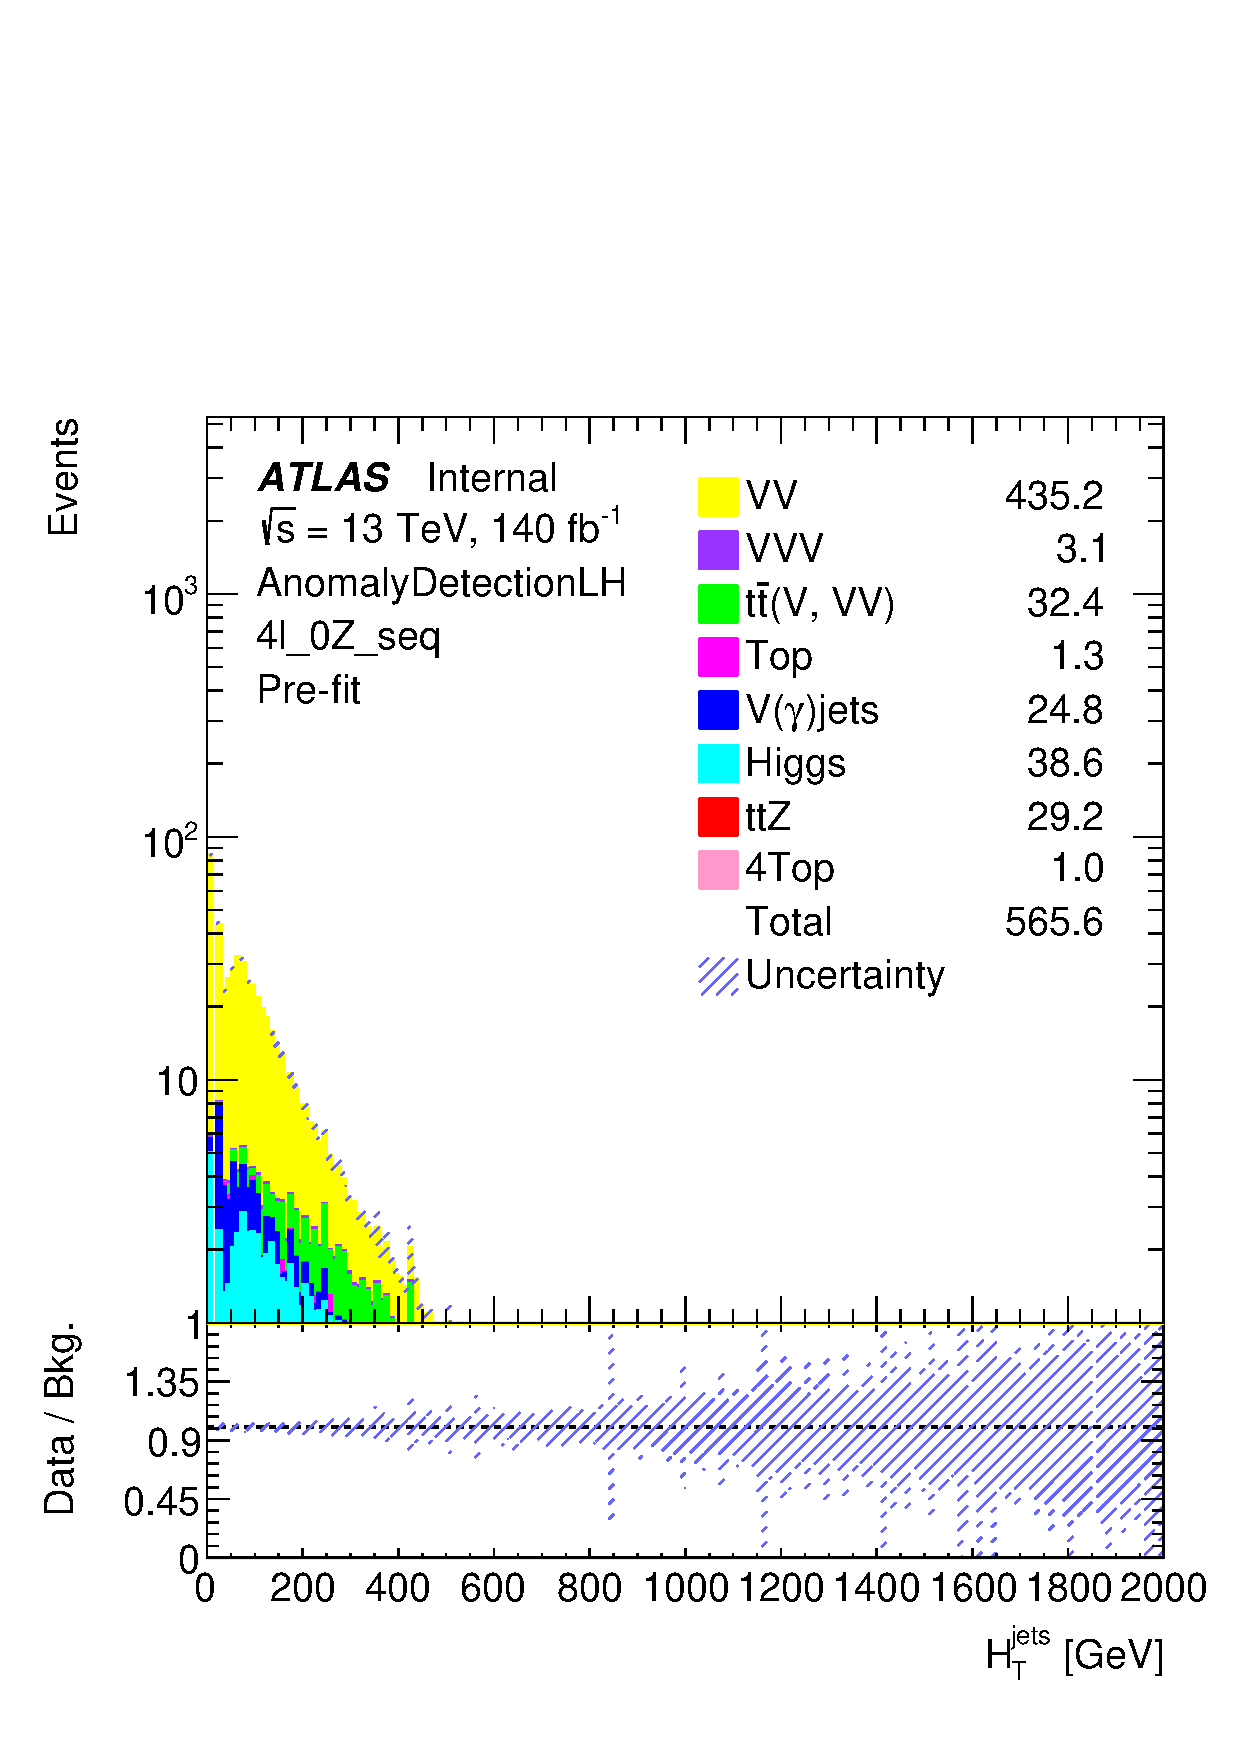
\includegraphics[width=0.24\textwidth]{plots/fourlepLH_run2/Plots/reg_4l_0Z_seq_HT_jets.pdf} &
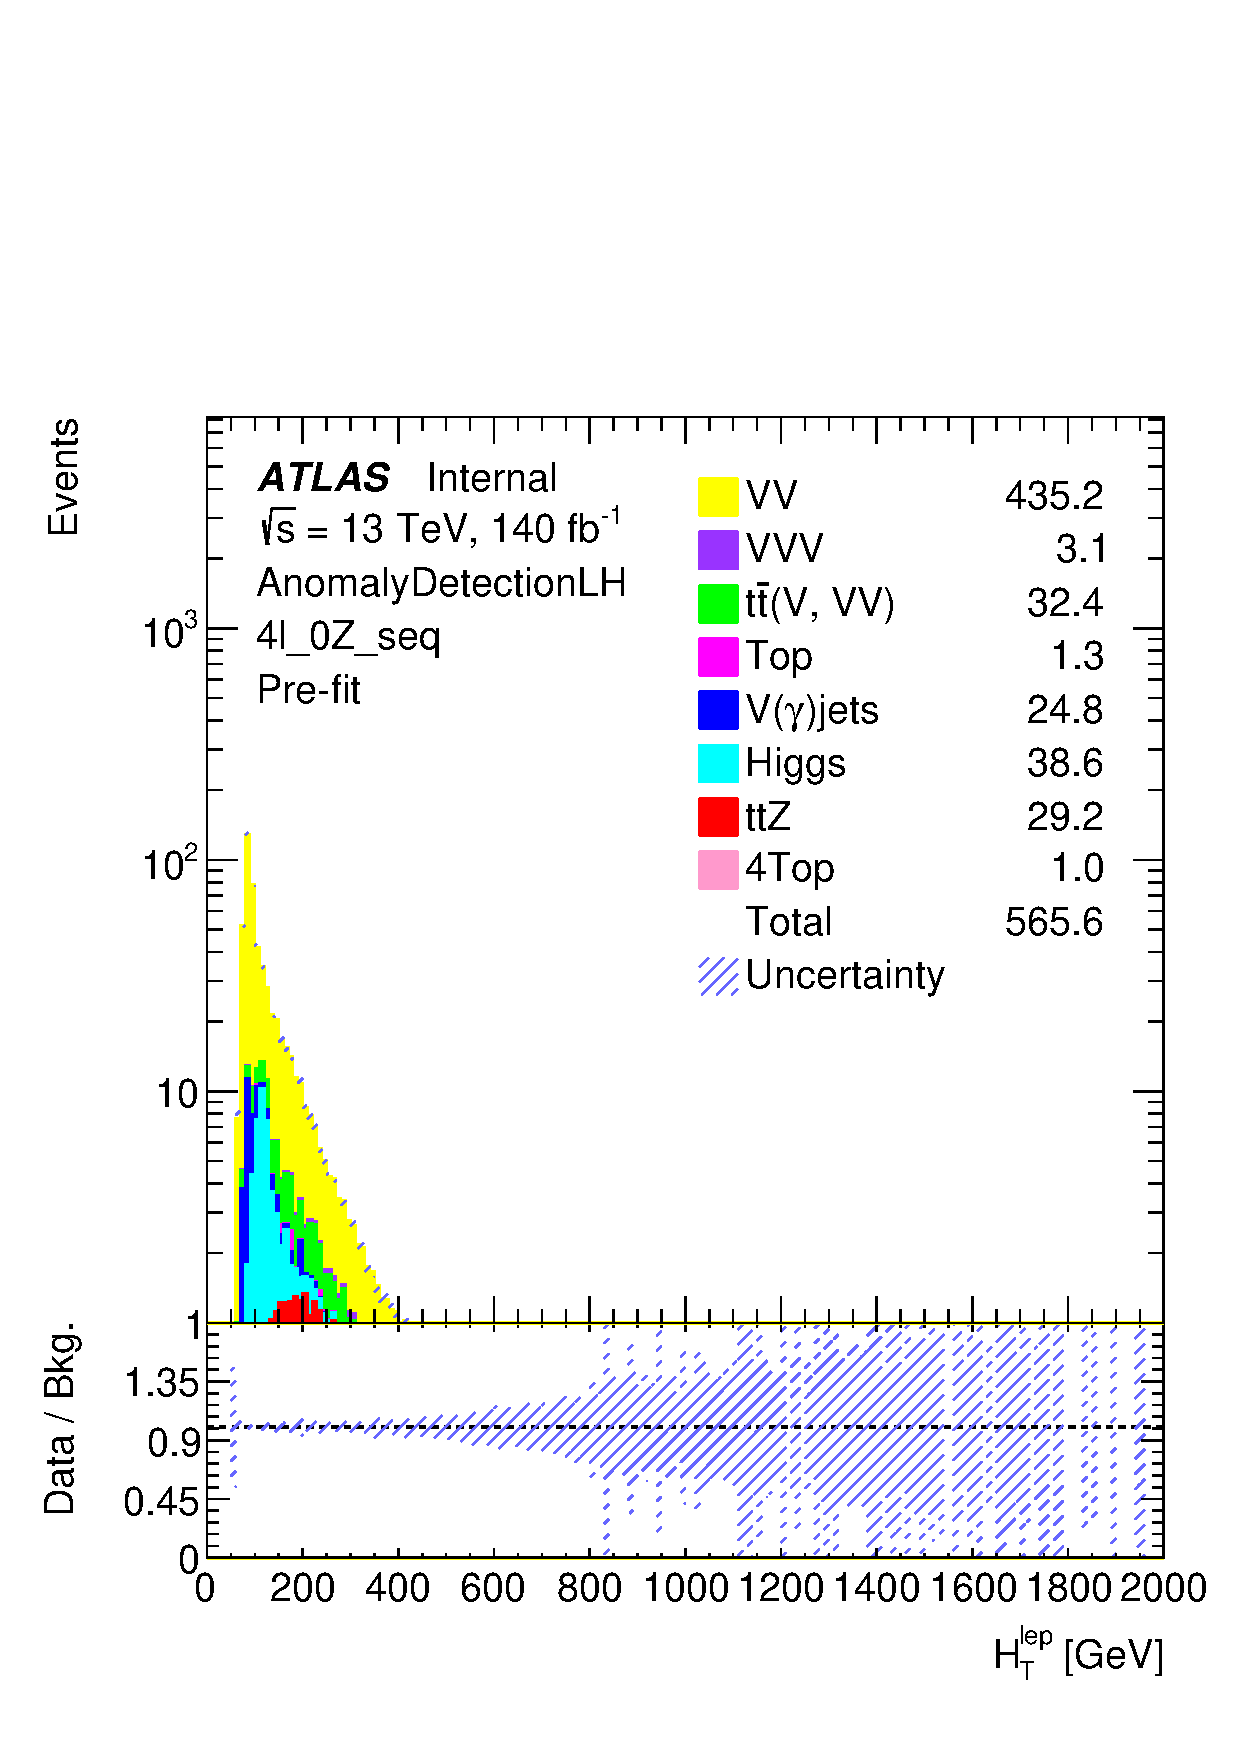
\includegraphics[width=0.24\textwidth]{plots/fourlepLH_run2/Plots/reg_4l_0Z_seq_HT_lep.pdf} &
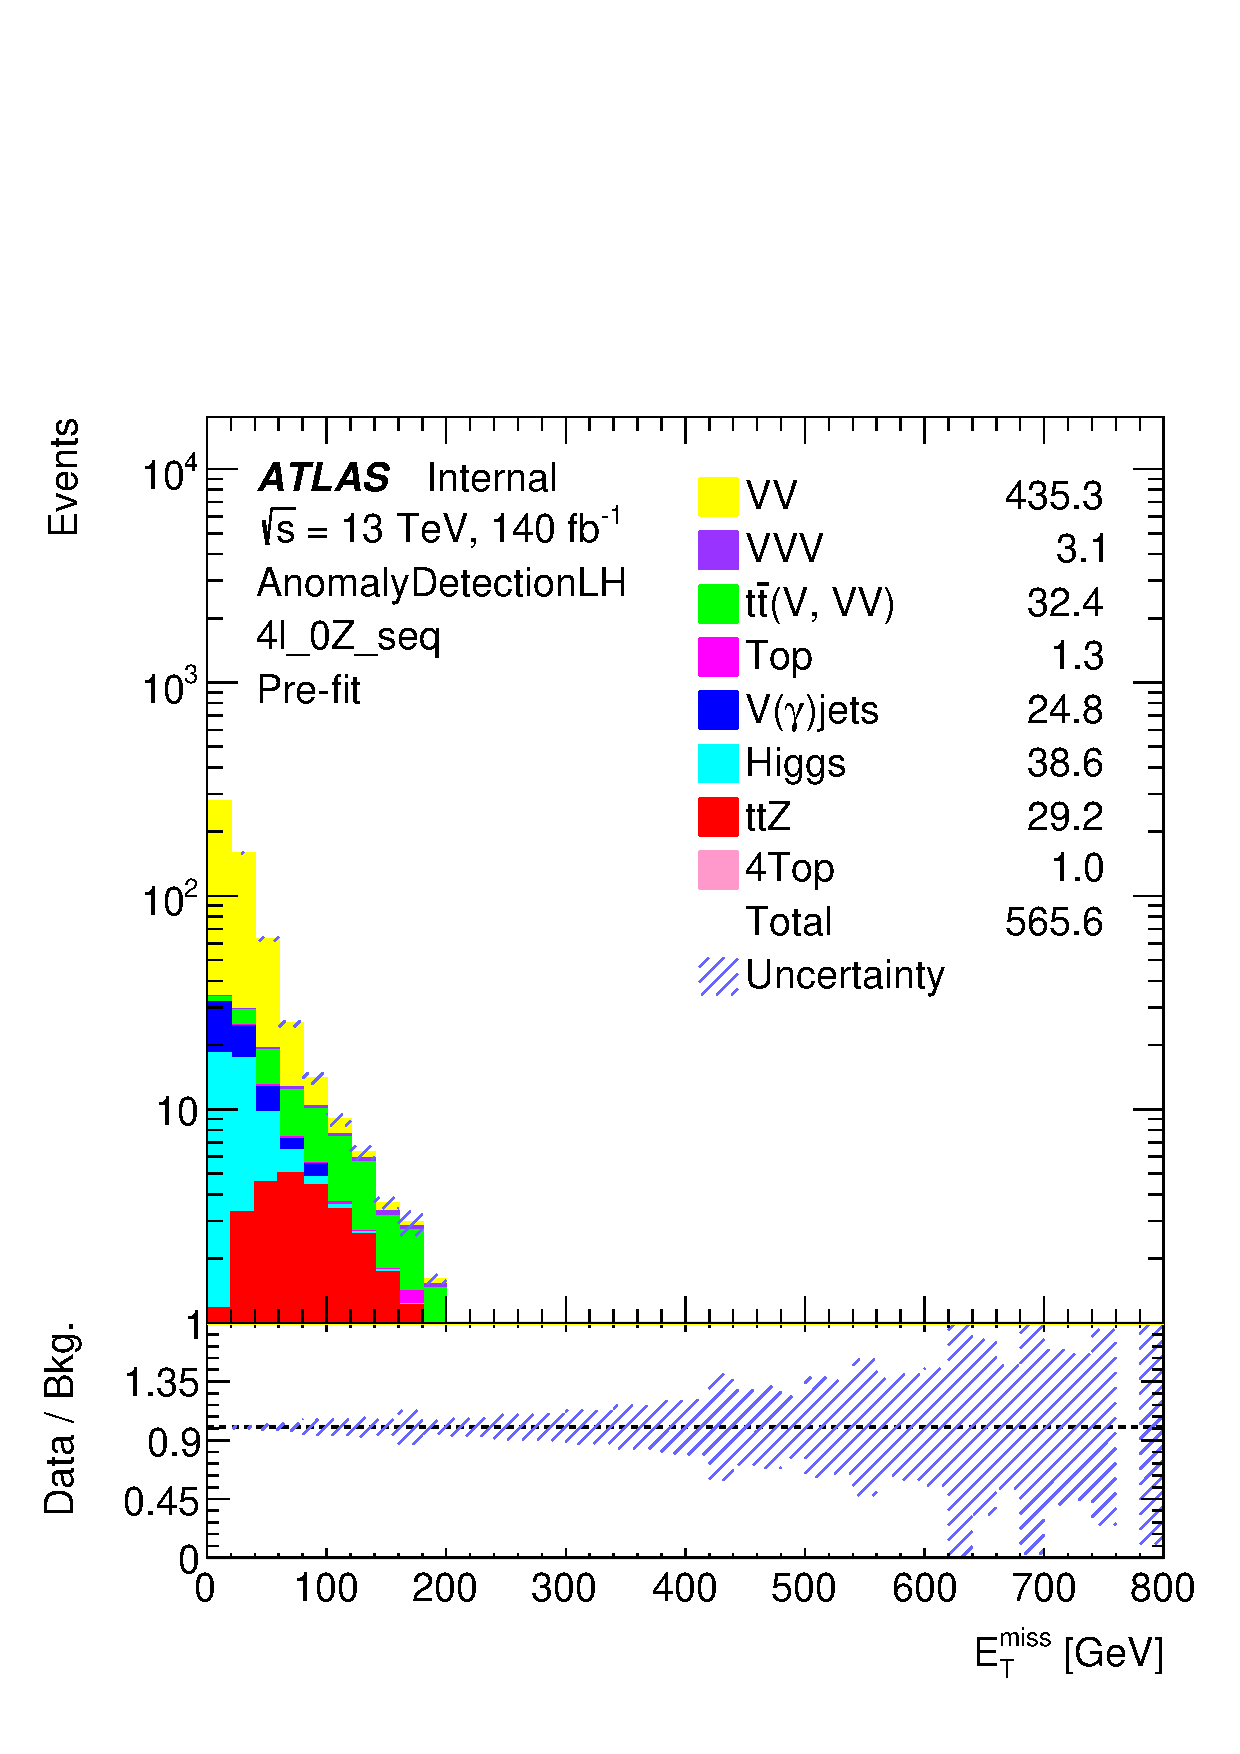
\includegraphics[width=0.24\textwidth]{plots/fourlepLH_run2/Plots/reg_4l_0Z_seq_met.pdf} \\

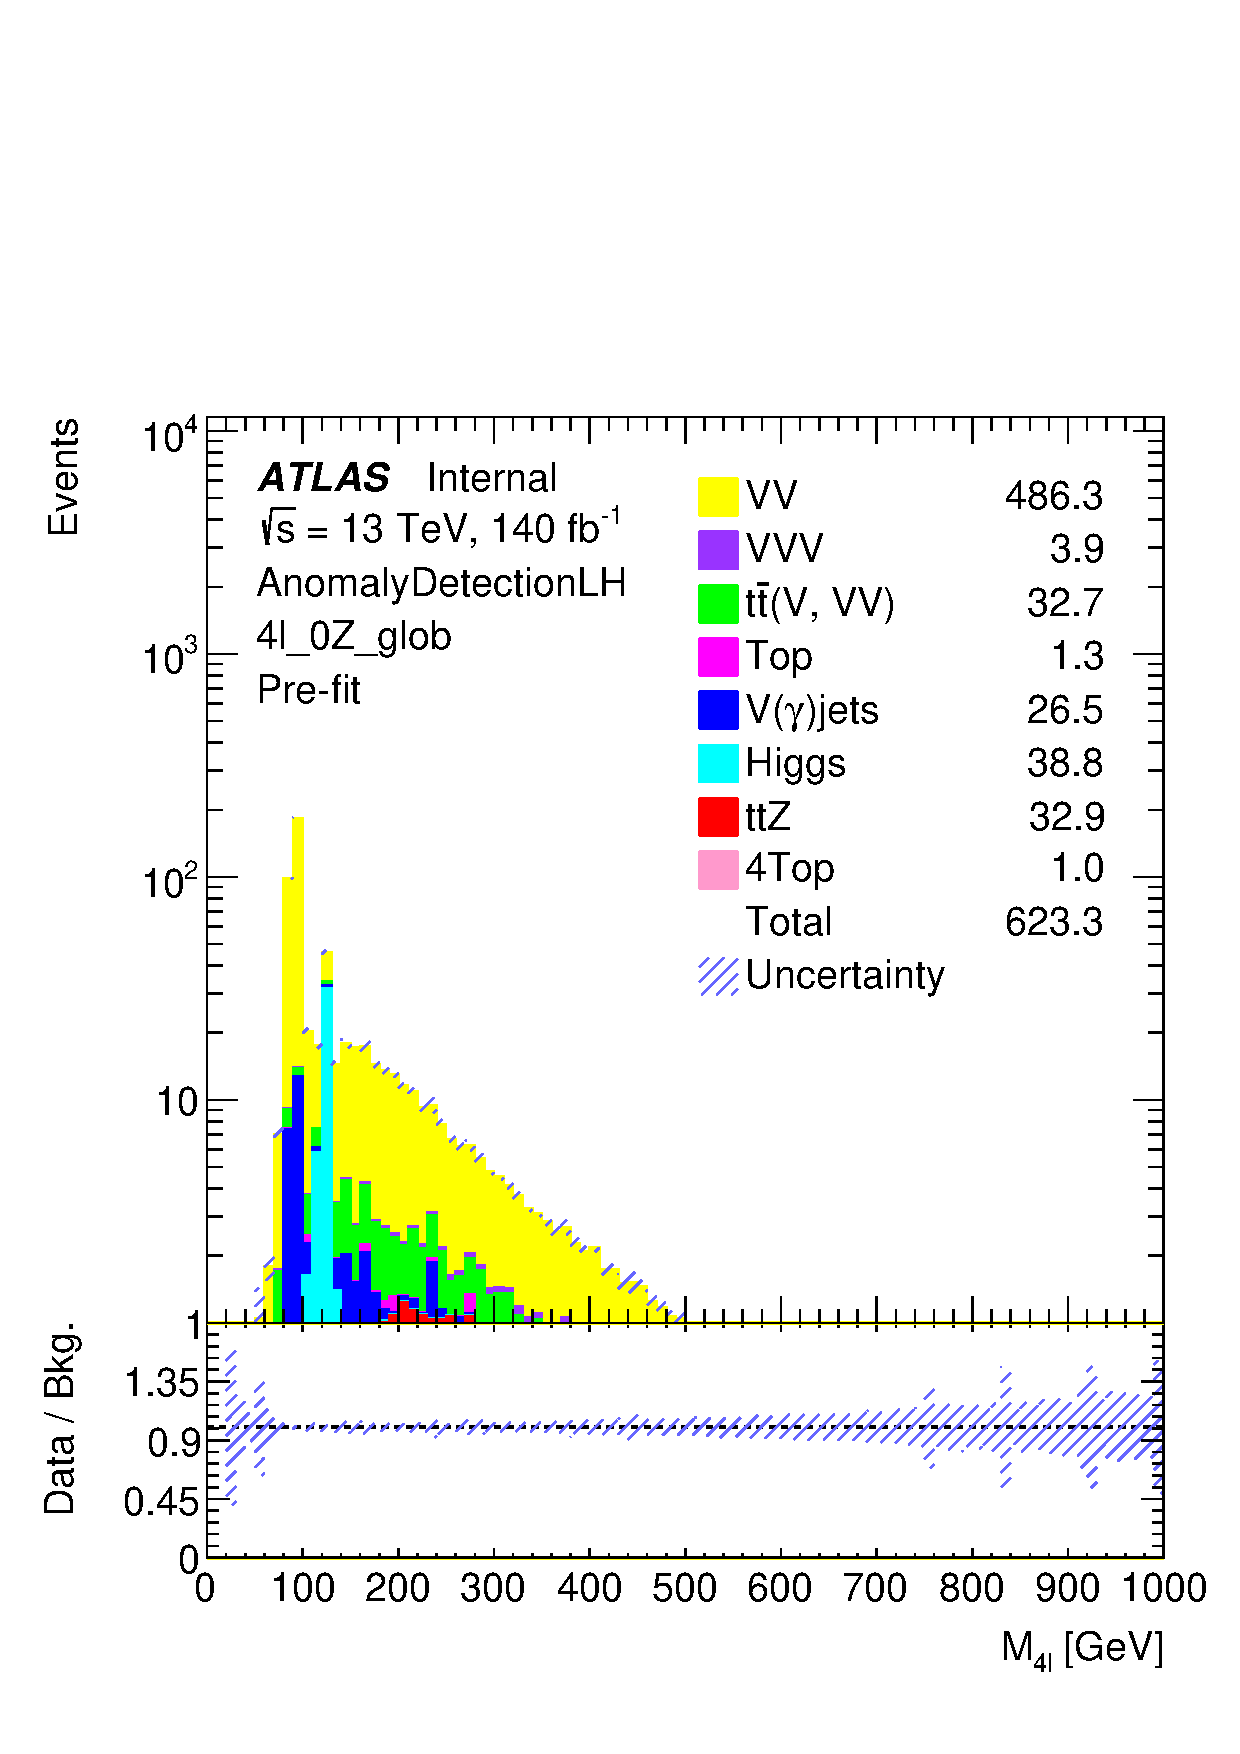
\includegraphics[width=0.24\textwidth]{plots/fourlepLH_run2/Plots/reg_4l_0Z_glob_m4l.pdf} &
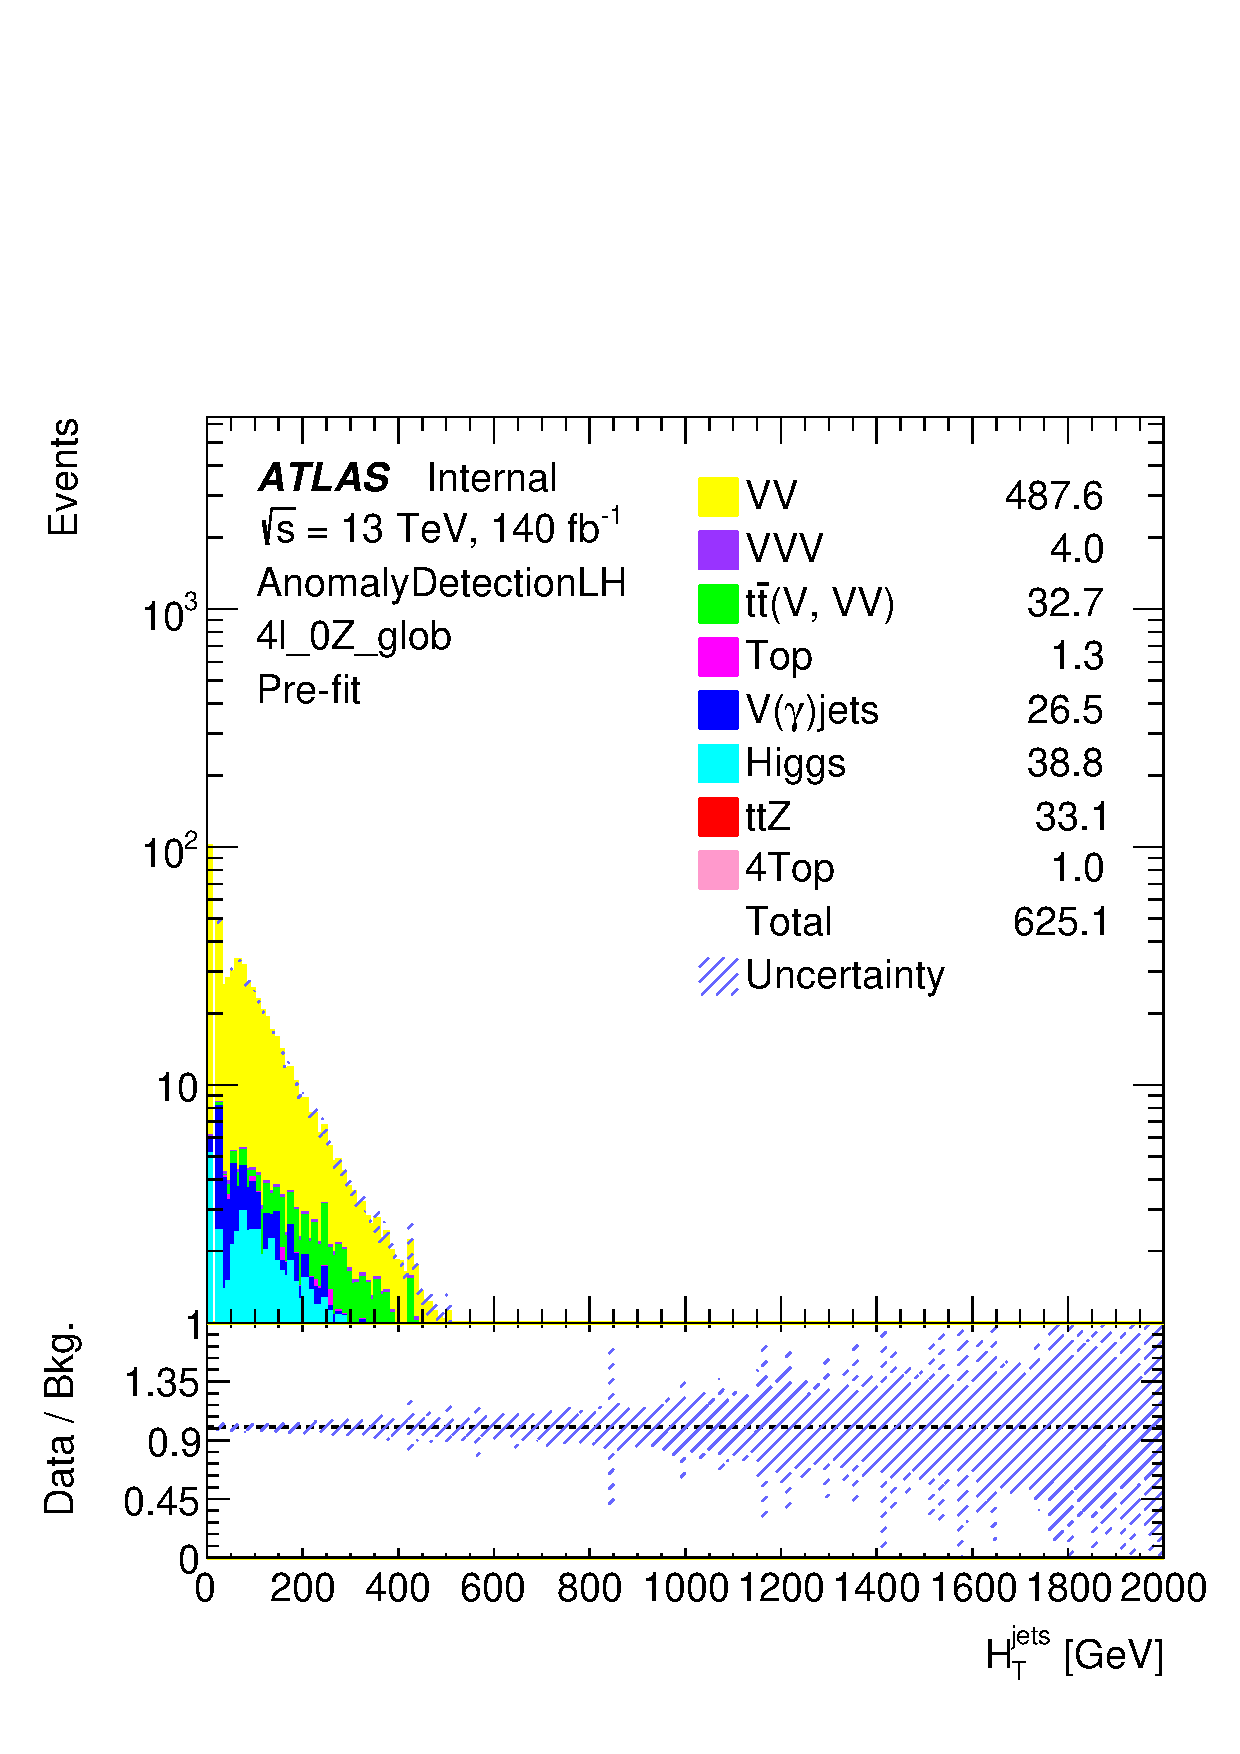
\includegraphics[width=0.24\textwidth]{plots/fourlepLH_run2/Plots/reg_4l_0Z_glob_HT_jets.pdf} &
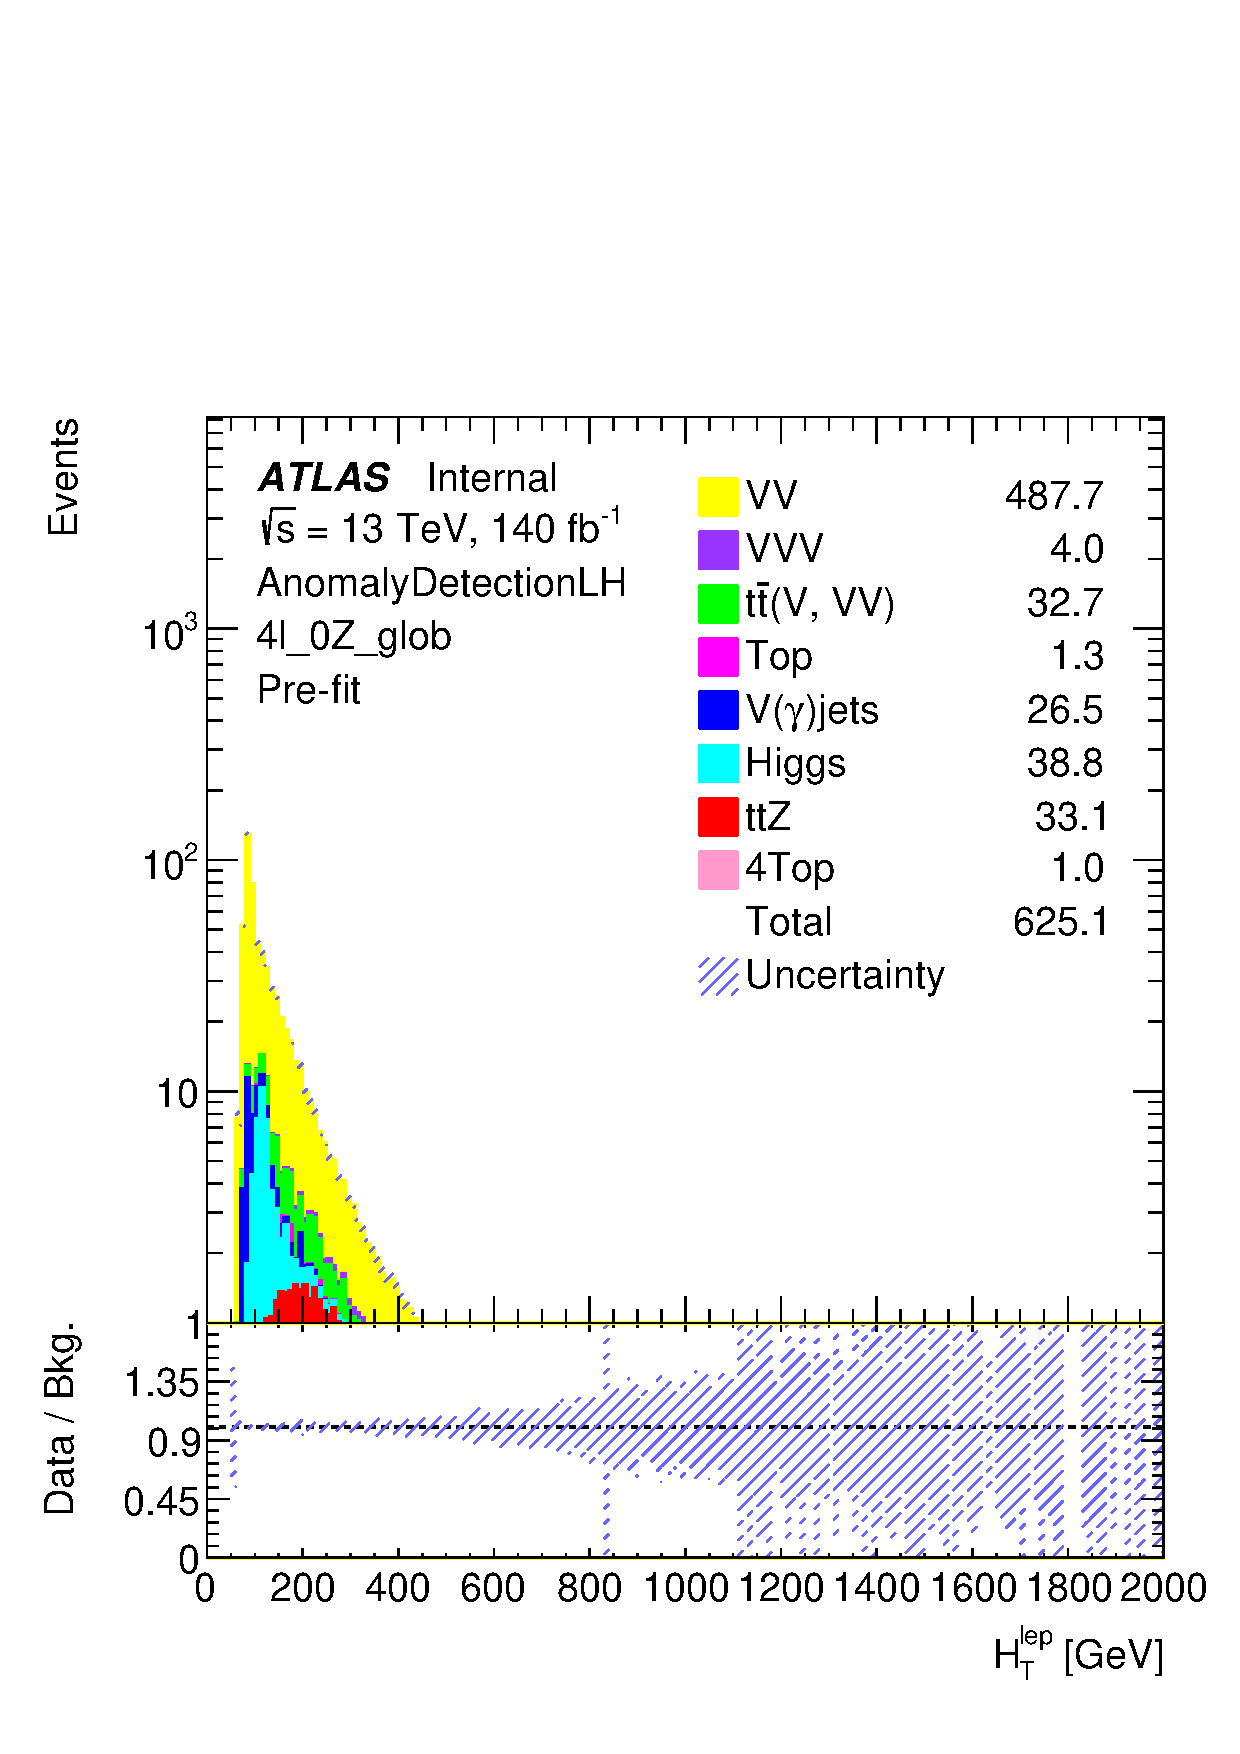
\includegraphics[width=0.24\textwidth]{plots/fourlepLH_run2/Plots/reg_4l_0Z_glob_HT_lep.pdf} &
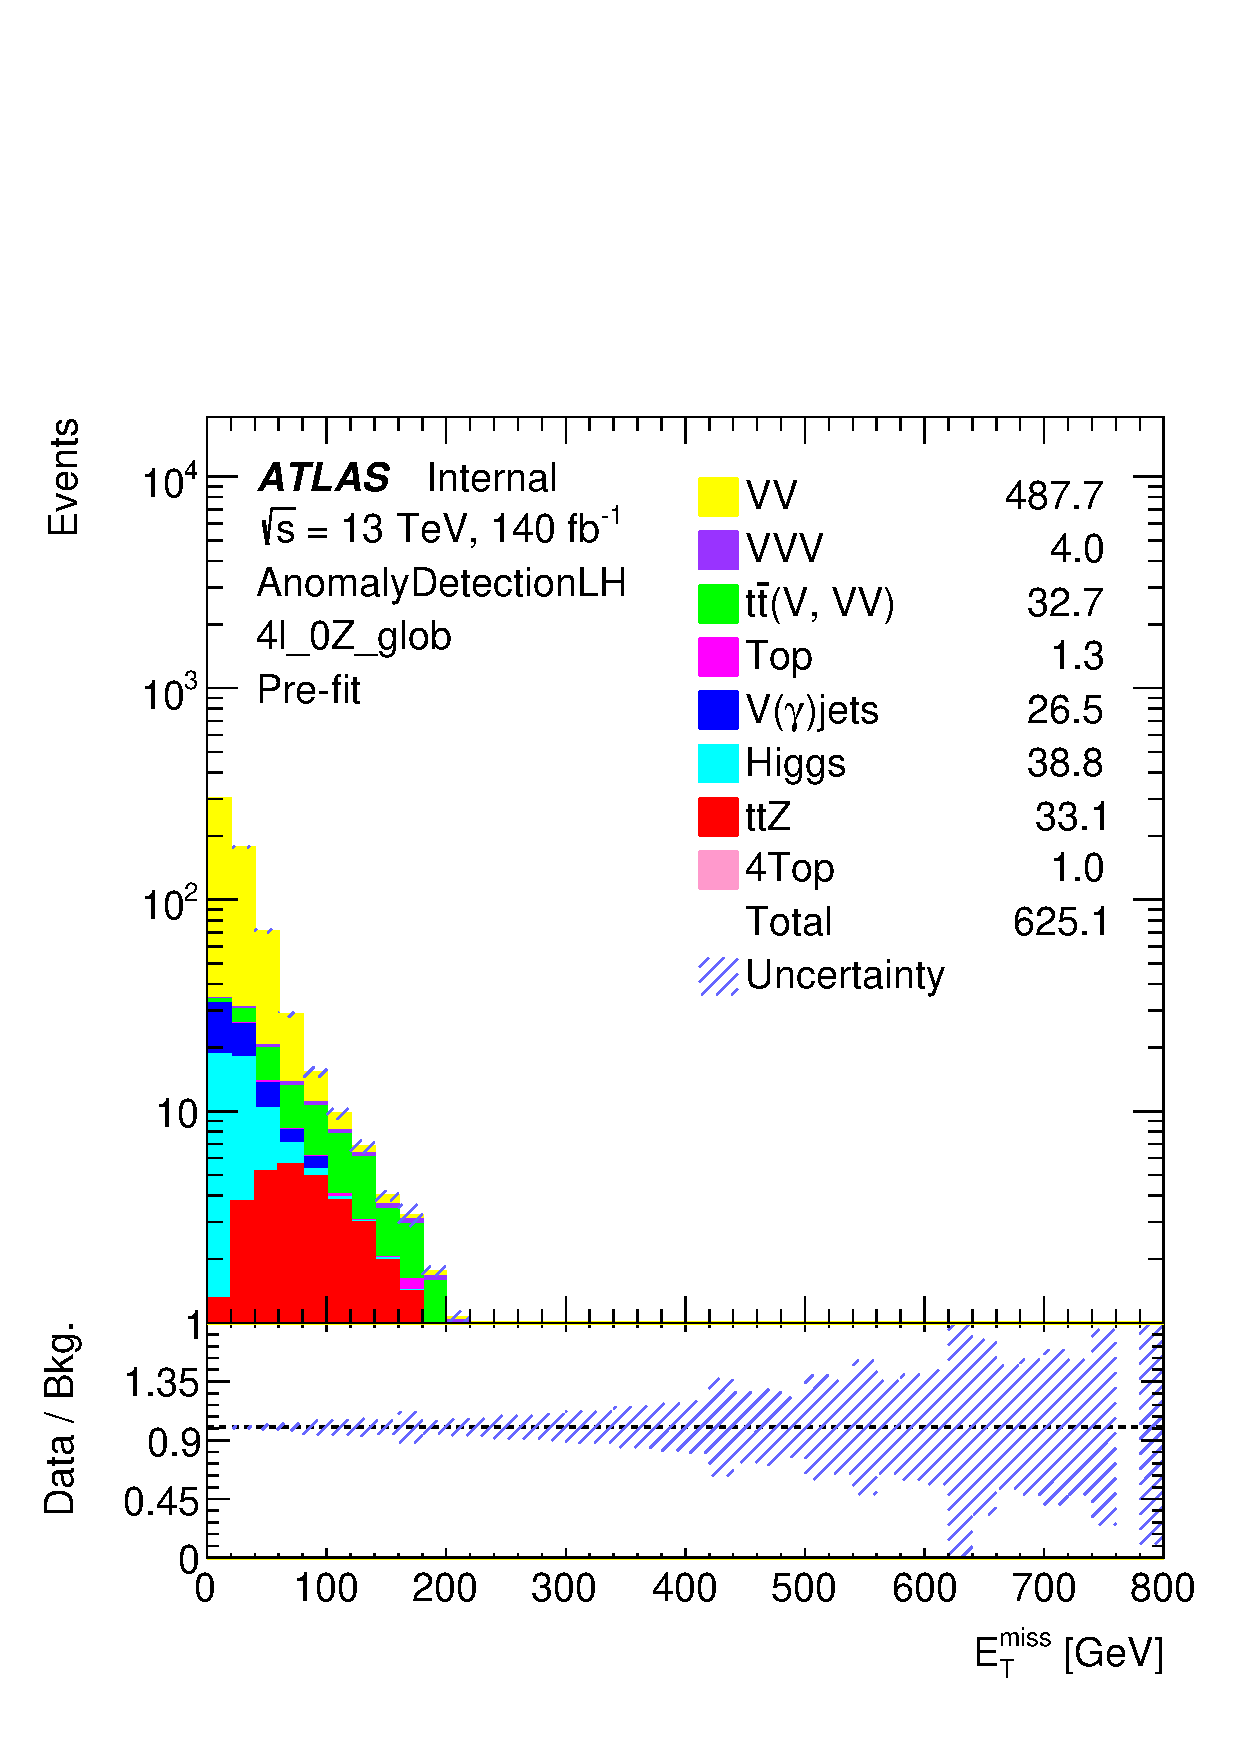
\includegraphics[width=0.24\textwidth]{plots/fourlepLH_run2/Plots/reg_4l_0Z_glob_met.pdf} \\

\end{tabular}
\end{frame}

\begin{frame}{\texttt{Results: 4l\_0Z}}
\begin{tabular}{cccccc}
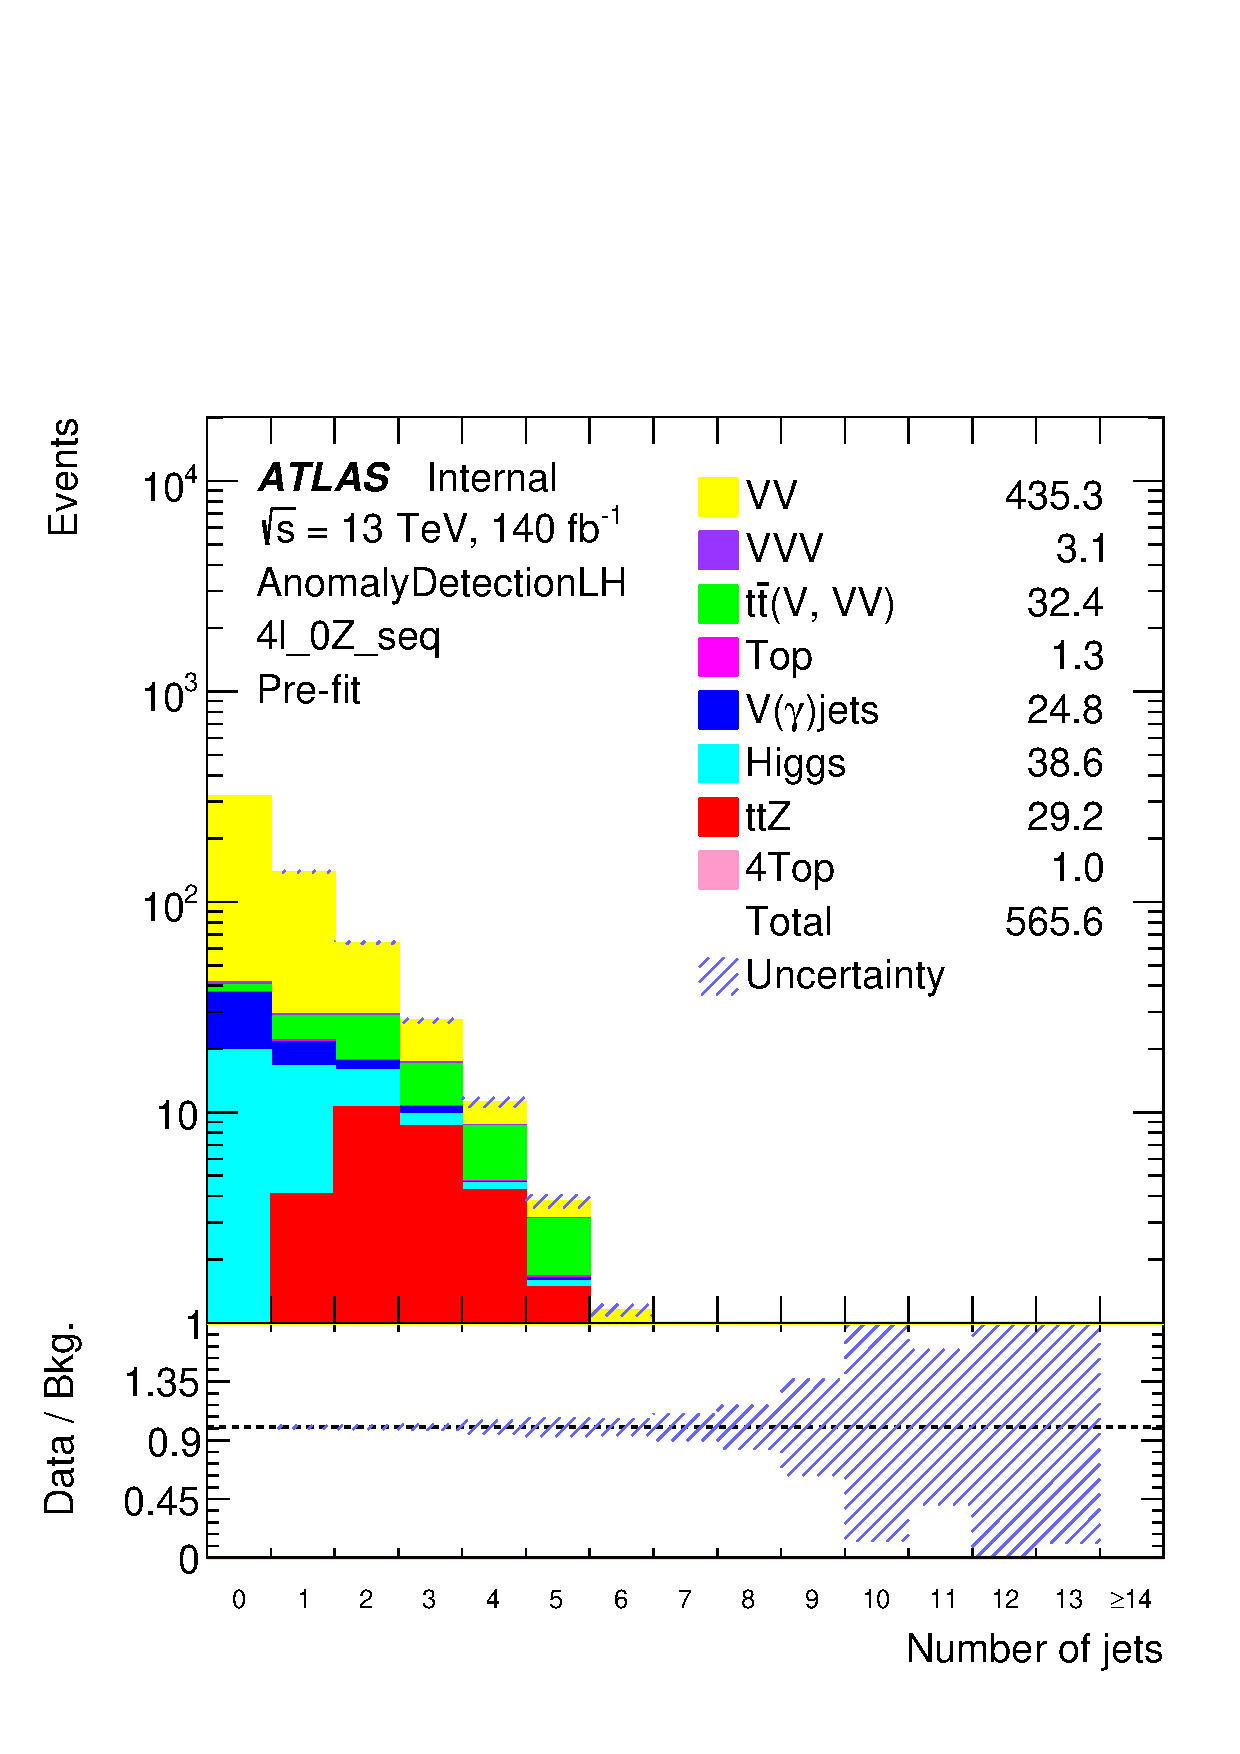
\includegraphics[width=0.24\textwidth]{plots/fourlepLH_run2/Plots/reg_4l_0Z_seq_nJets.pdf} &
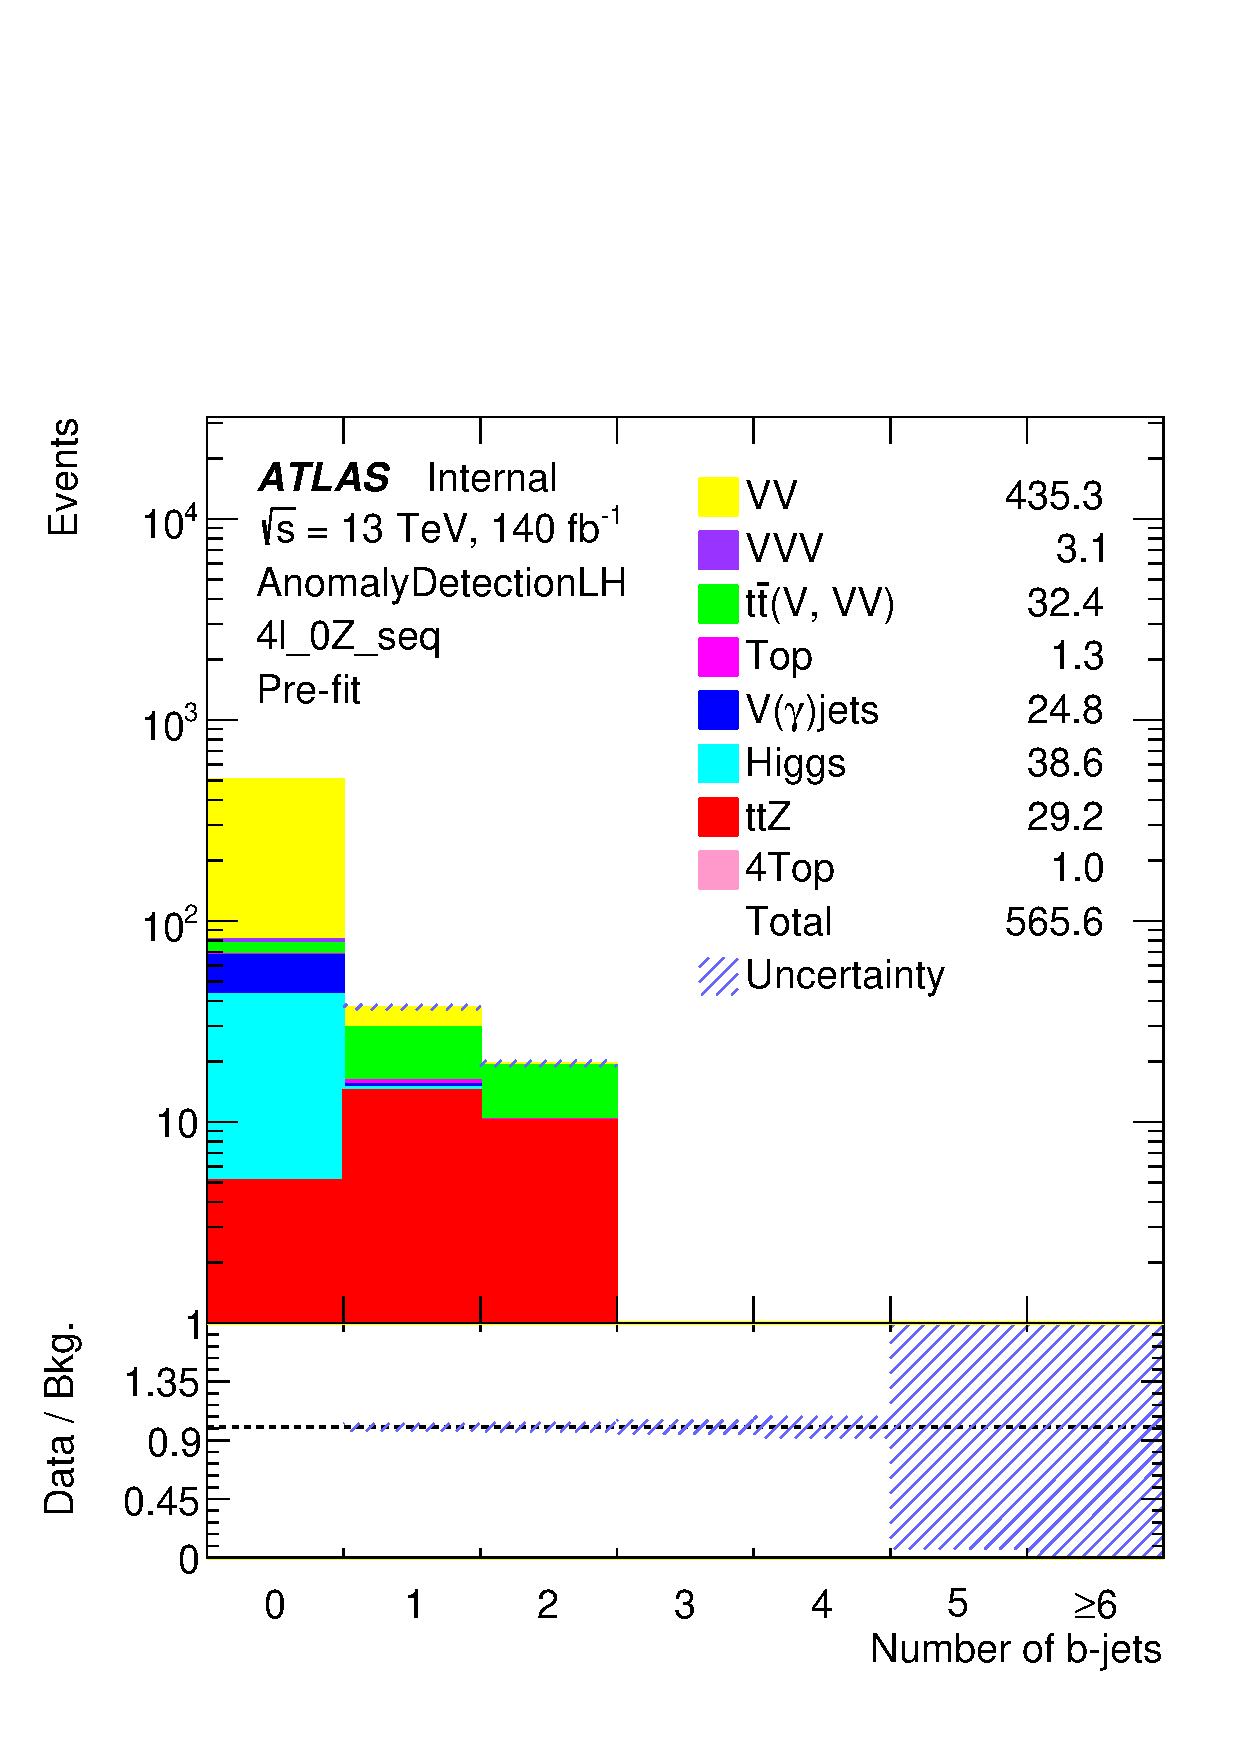
\includegraphics[width=0.24\textwidth]{plots/fourlepLH_run2/Plots/reg_4l_0Z_seq_nbJets.pdf} &
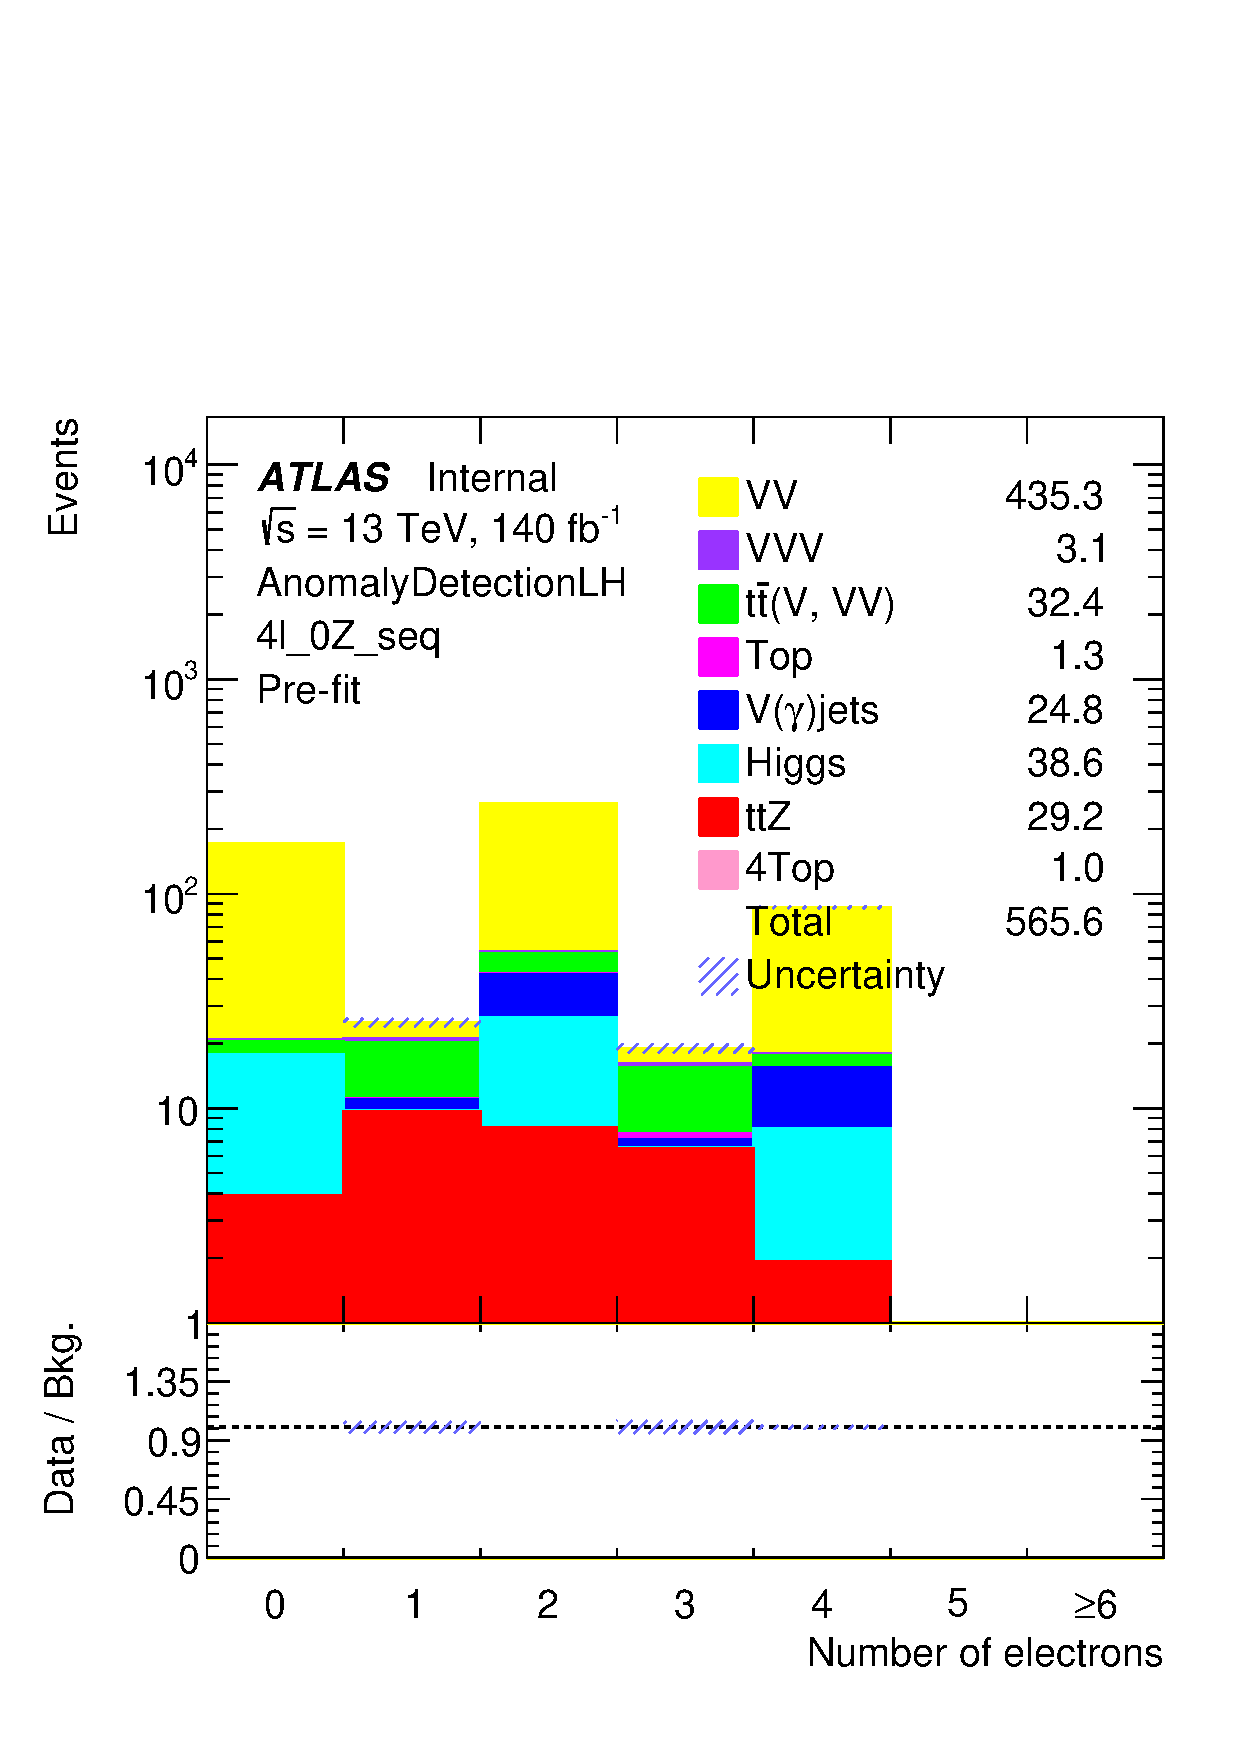
\includegraphics[width=0.24\textwidth]{plots/fourlepLH_run2/Plots/reg_4l_0Z_seq_nElectrons.pdf} &
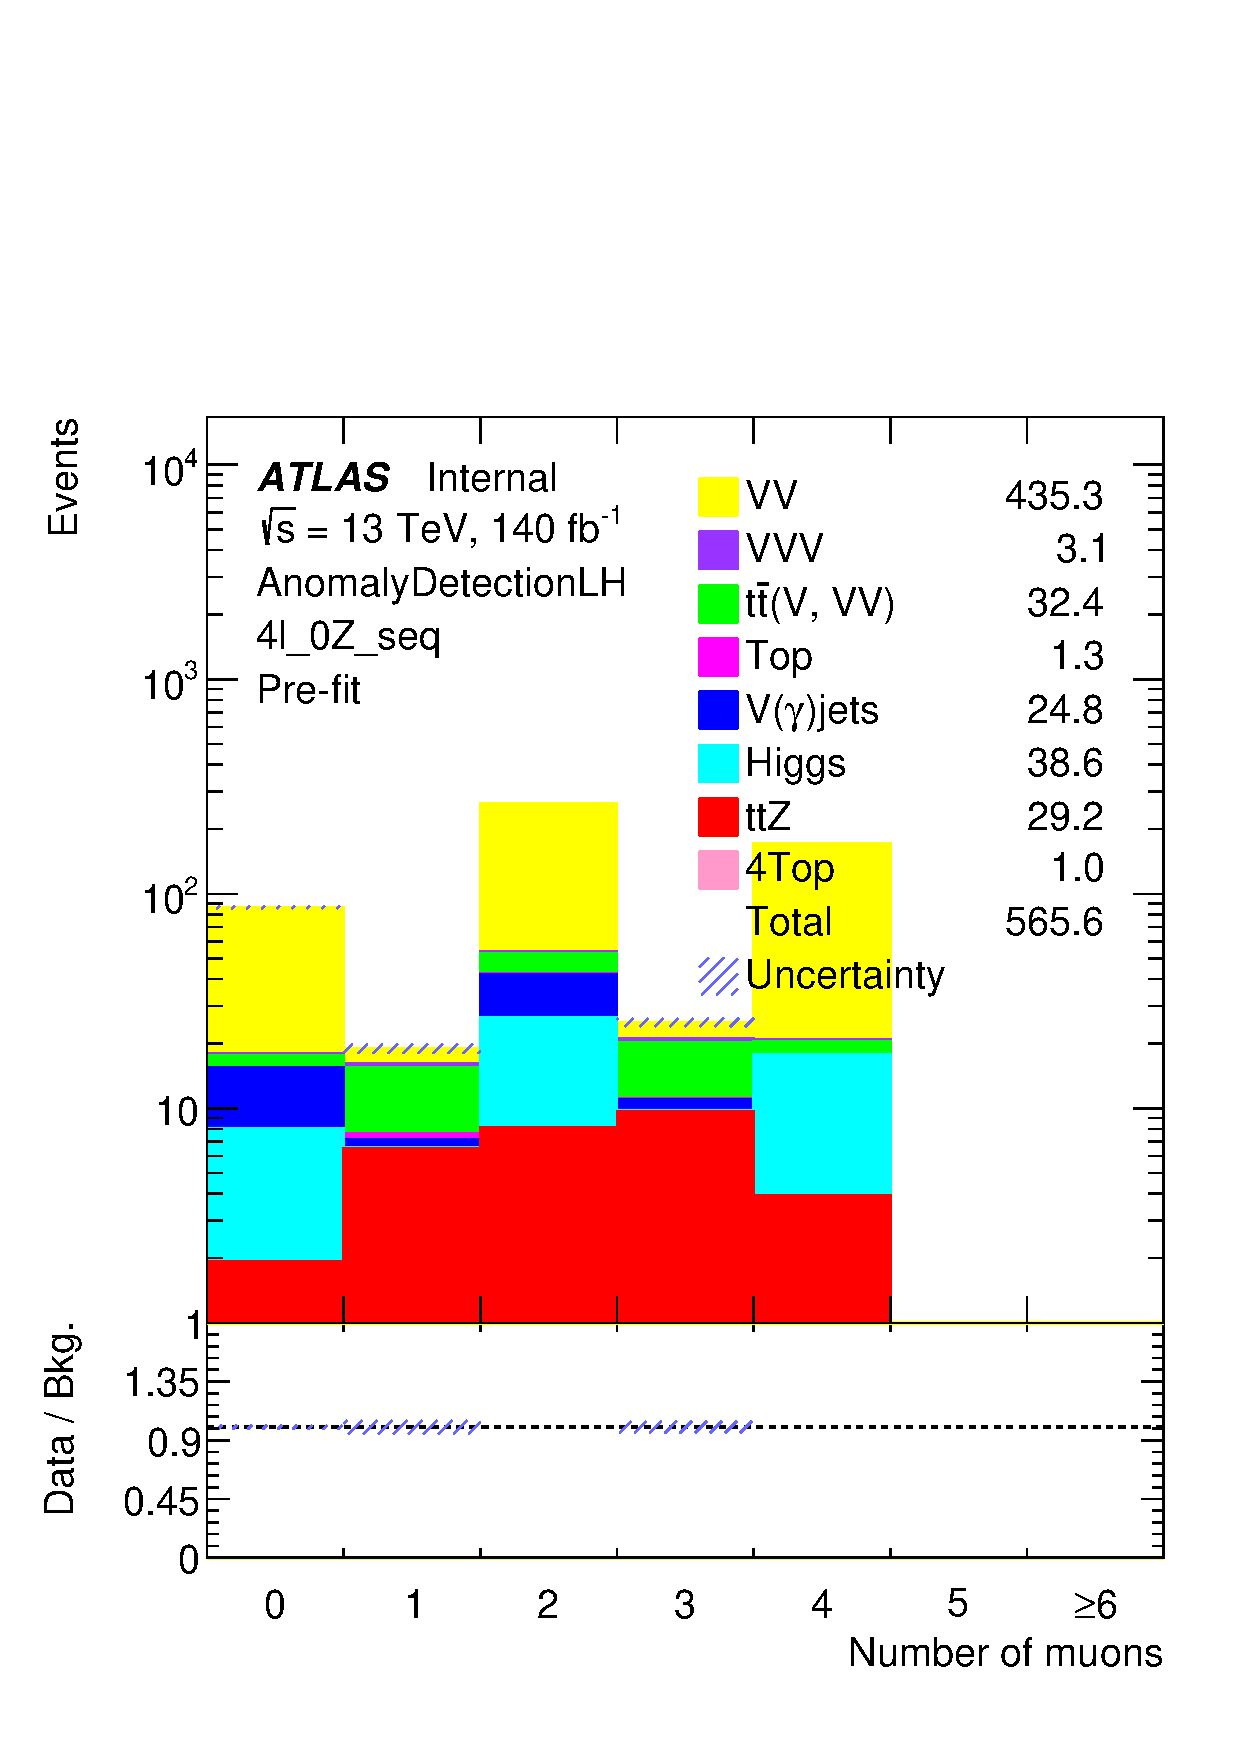
\includegraphics[width=0.24\textwidth]{plots/fourlepLH_run2/Plots/reg_4l_0Z_seq_nMuons.pdf} \\

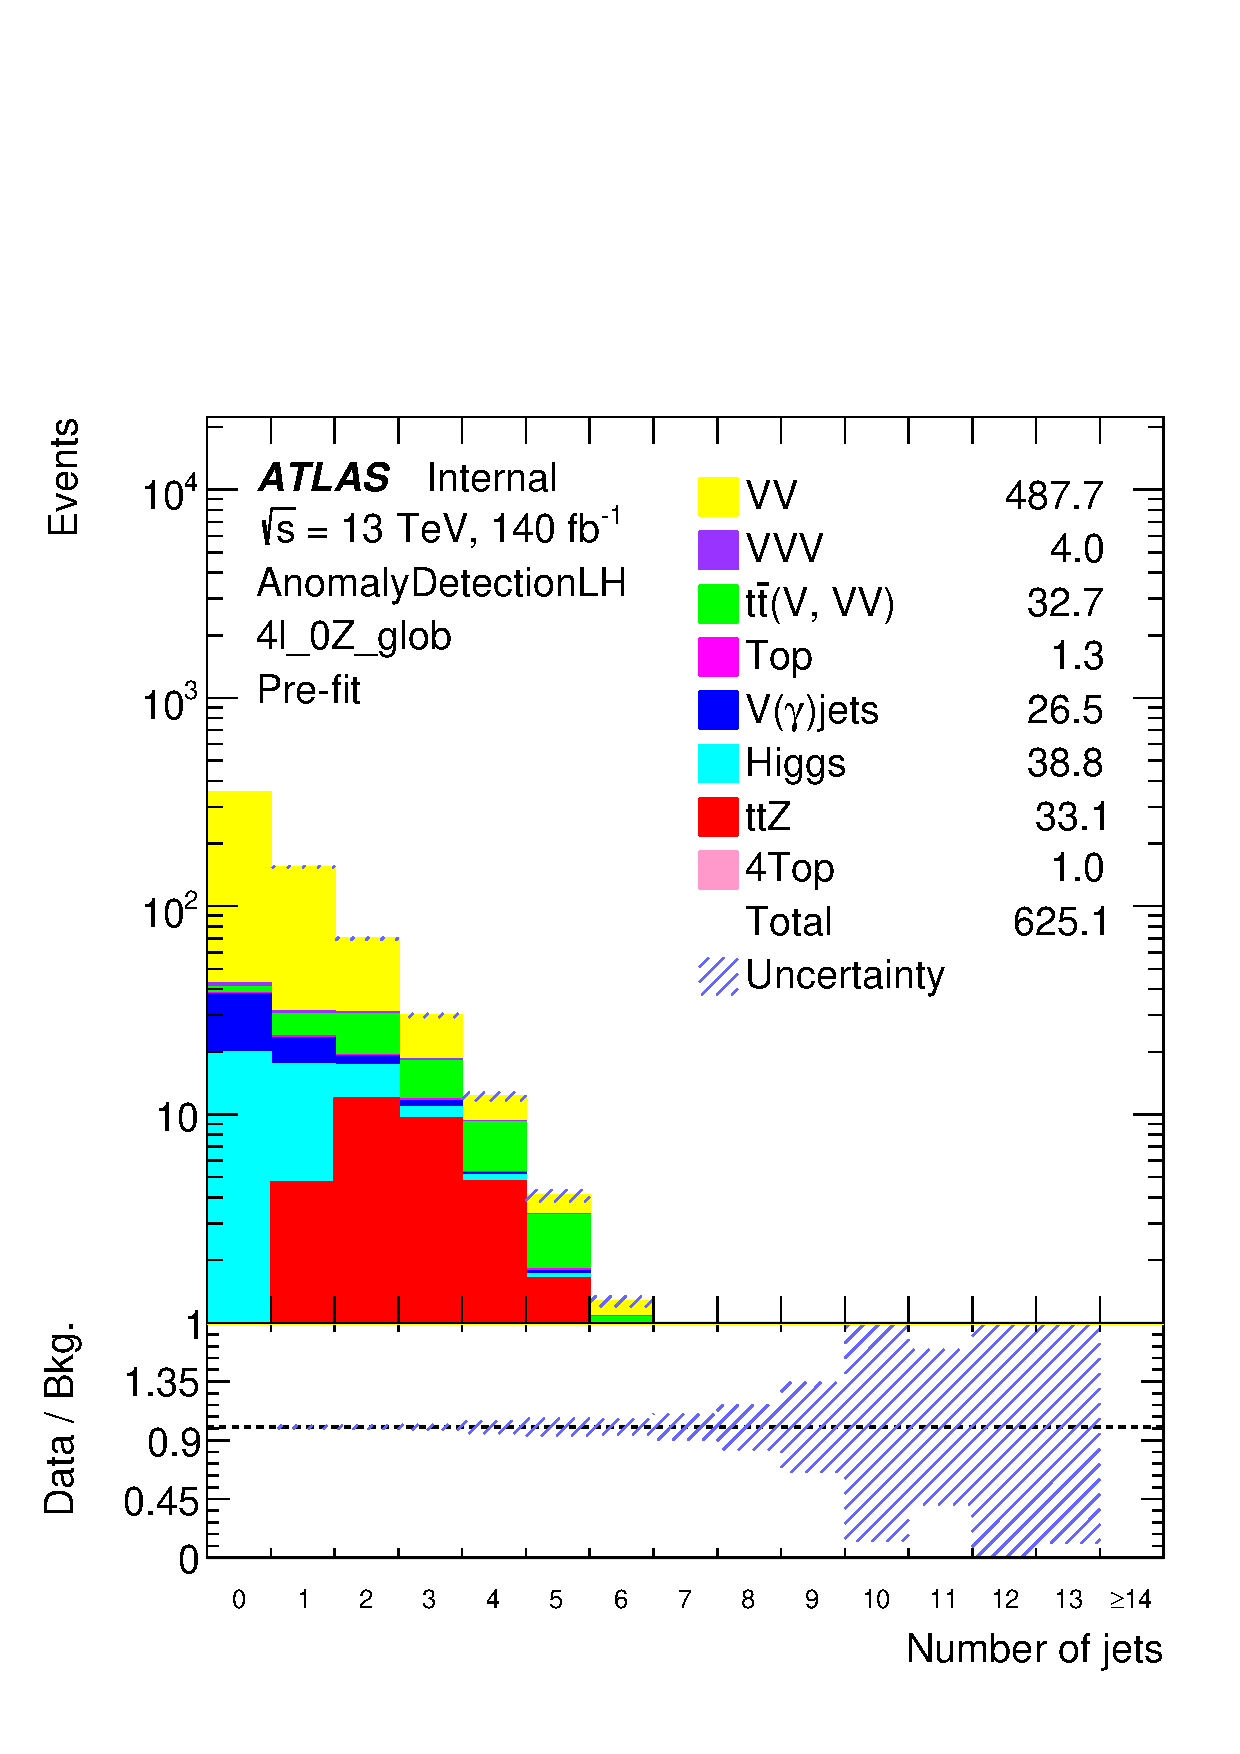
\includegraphics[width=0.24\textwidth]{plots/fourlepLH_run2/Plots/reg_4l_0Z_glob_nJets.pdf} &
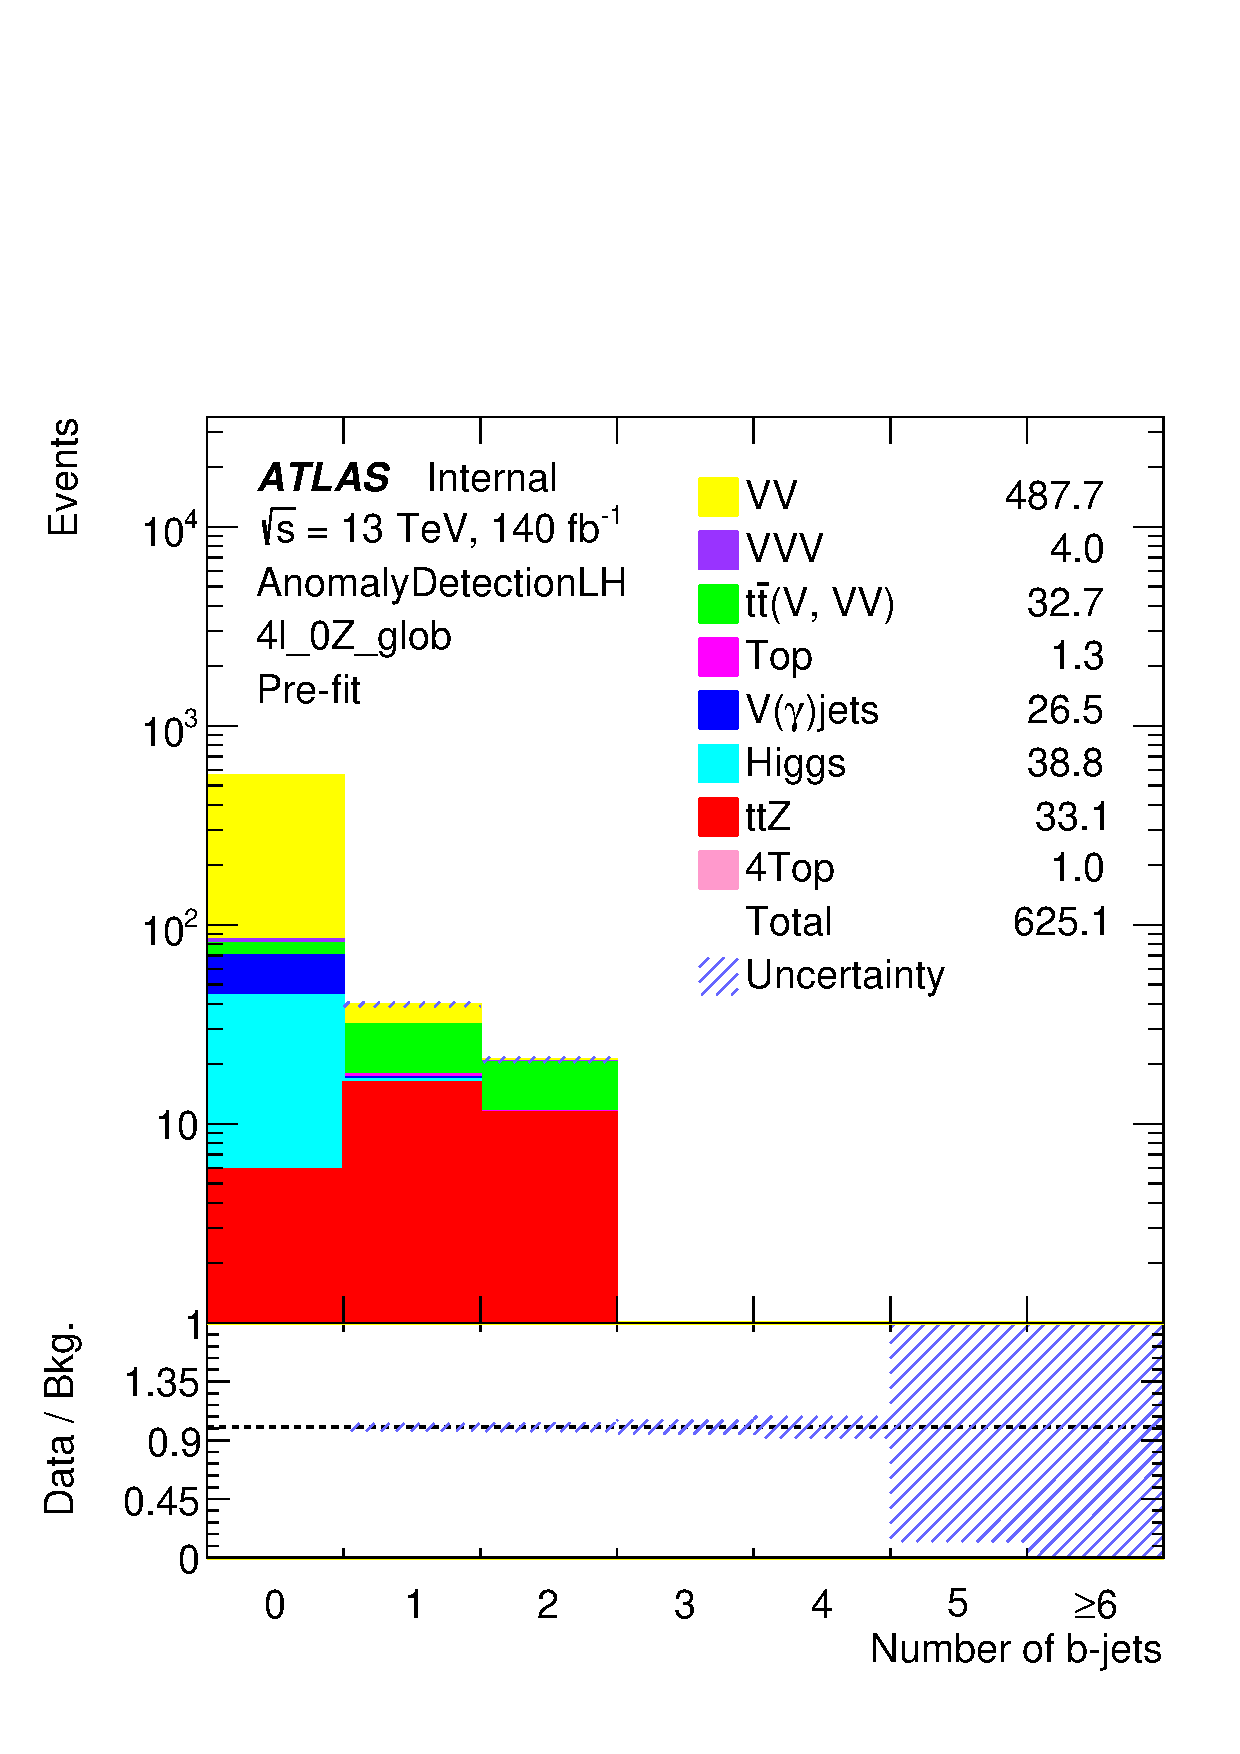
\includegraphics[width=0.24\textwidth]{plots/fourlepLH_run2/Plots/reg_4l_0Z_glob_nbJets.pdf} &
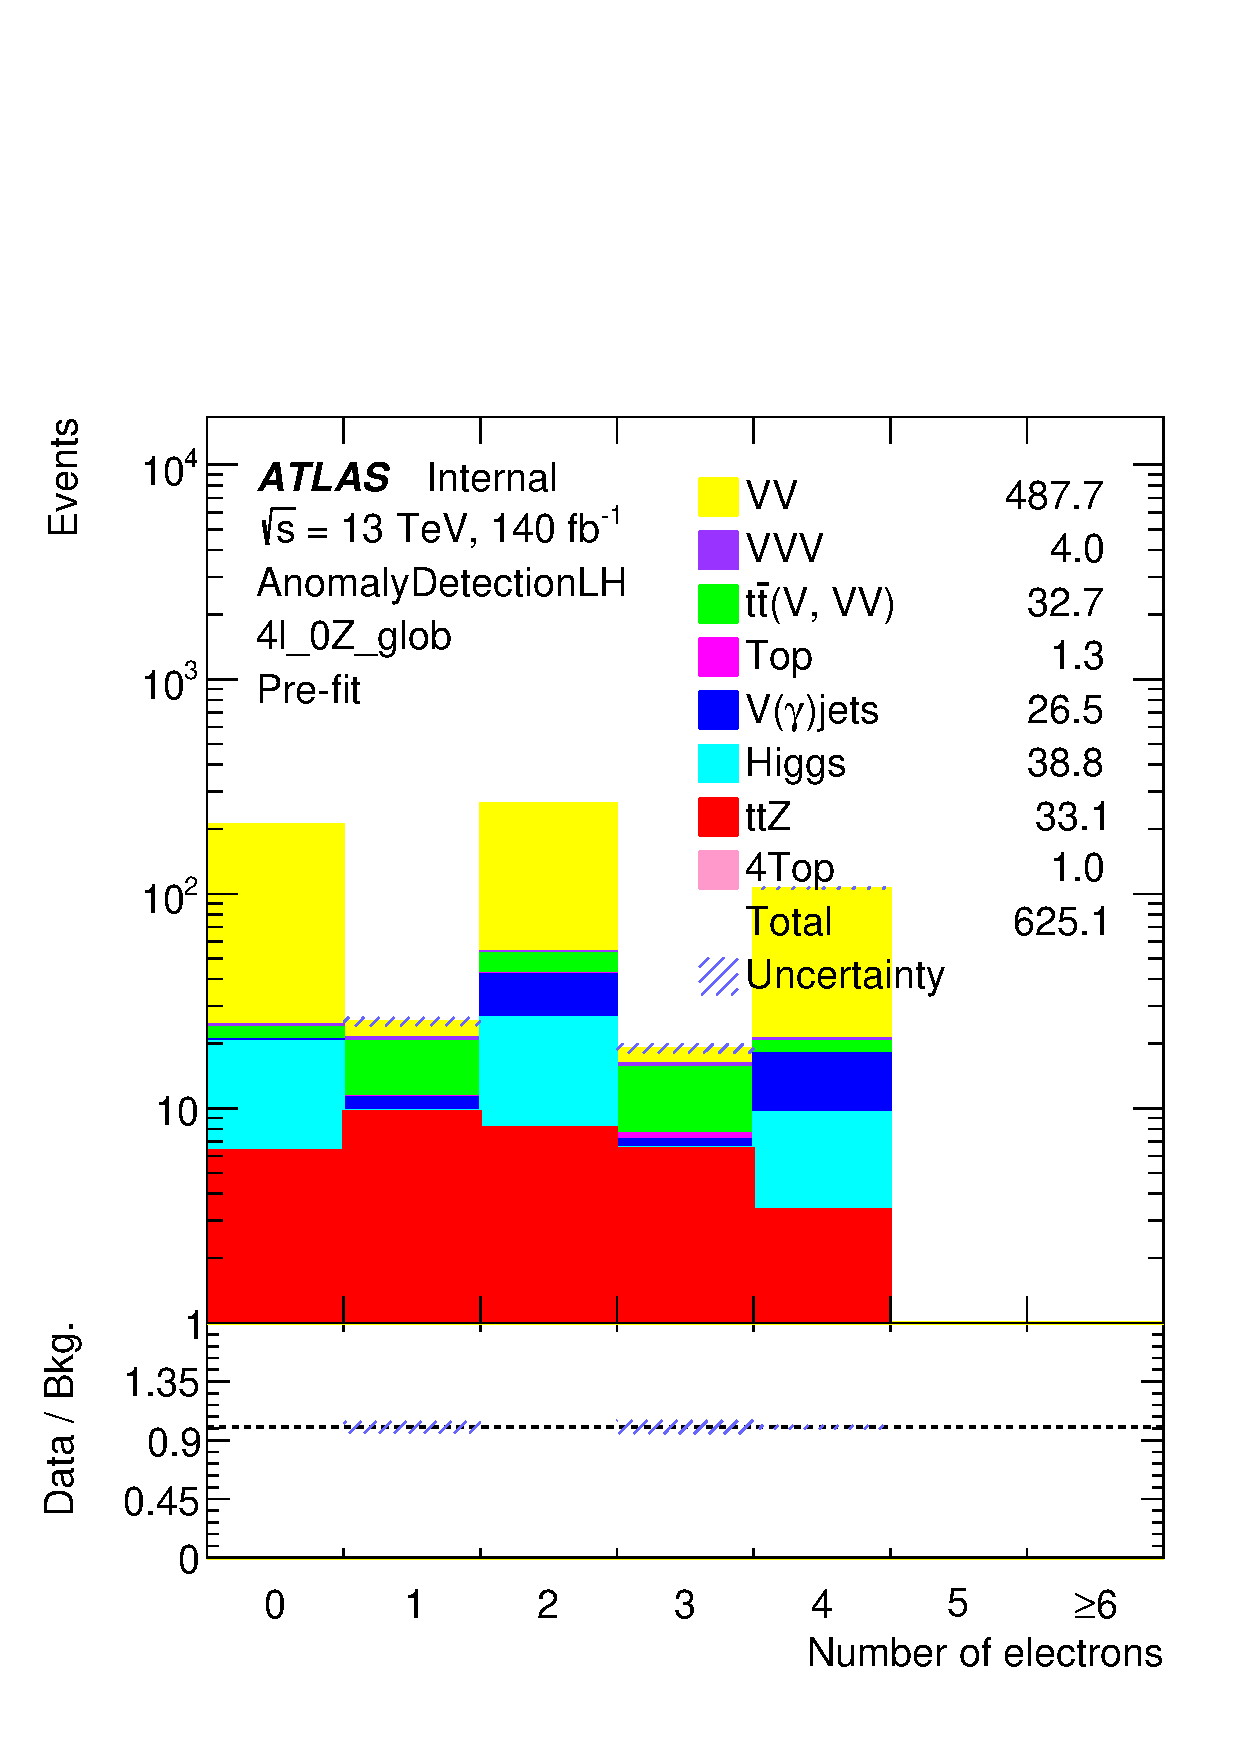
\includegraphics[width=0.24\textwidth]{plots/fourlepLH_run2/Plots/reg_4l_0Z_glob_nElectrons.pdf} &
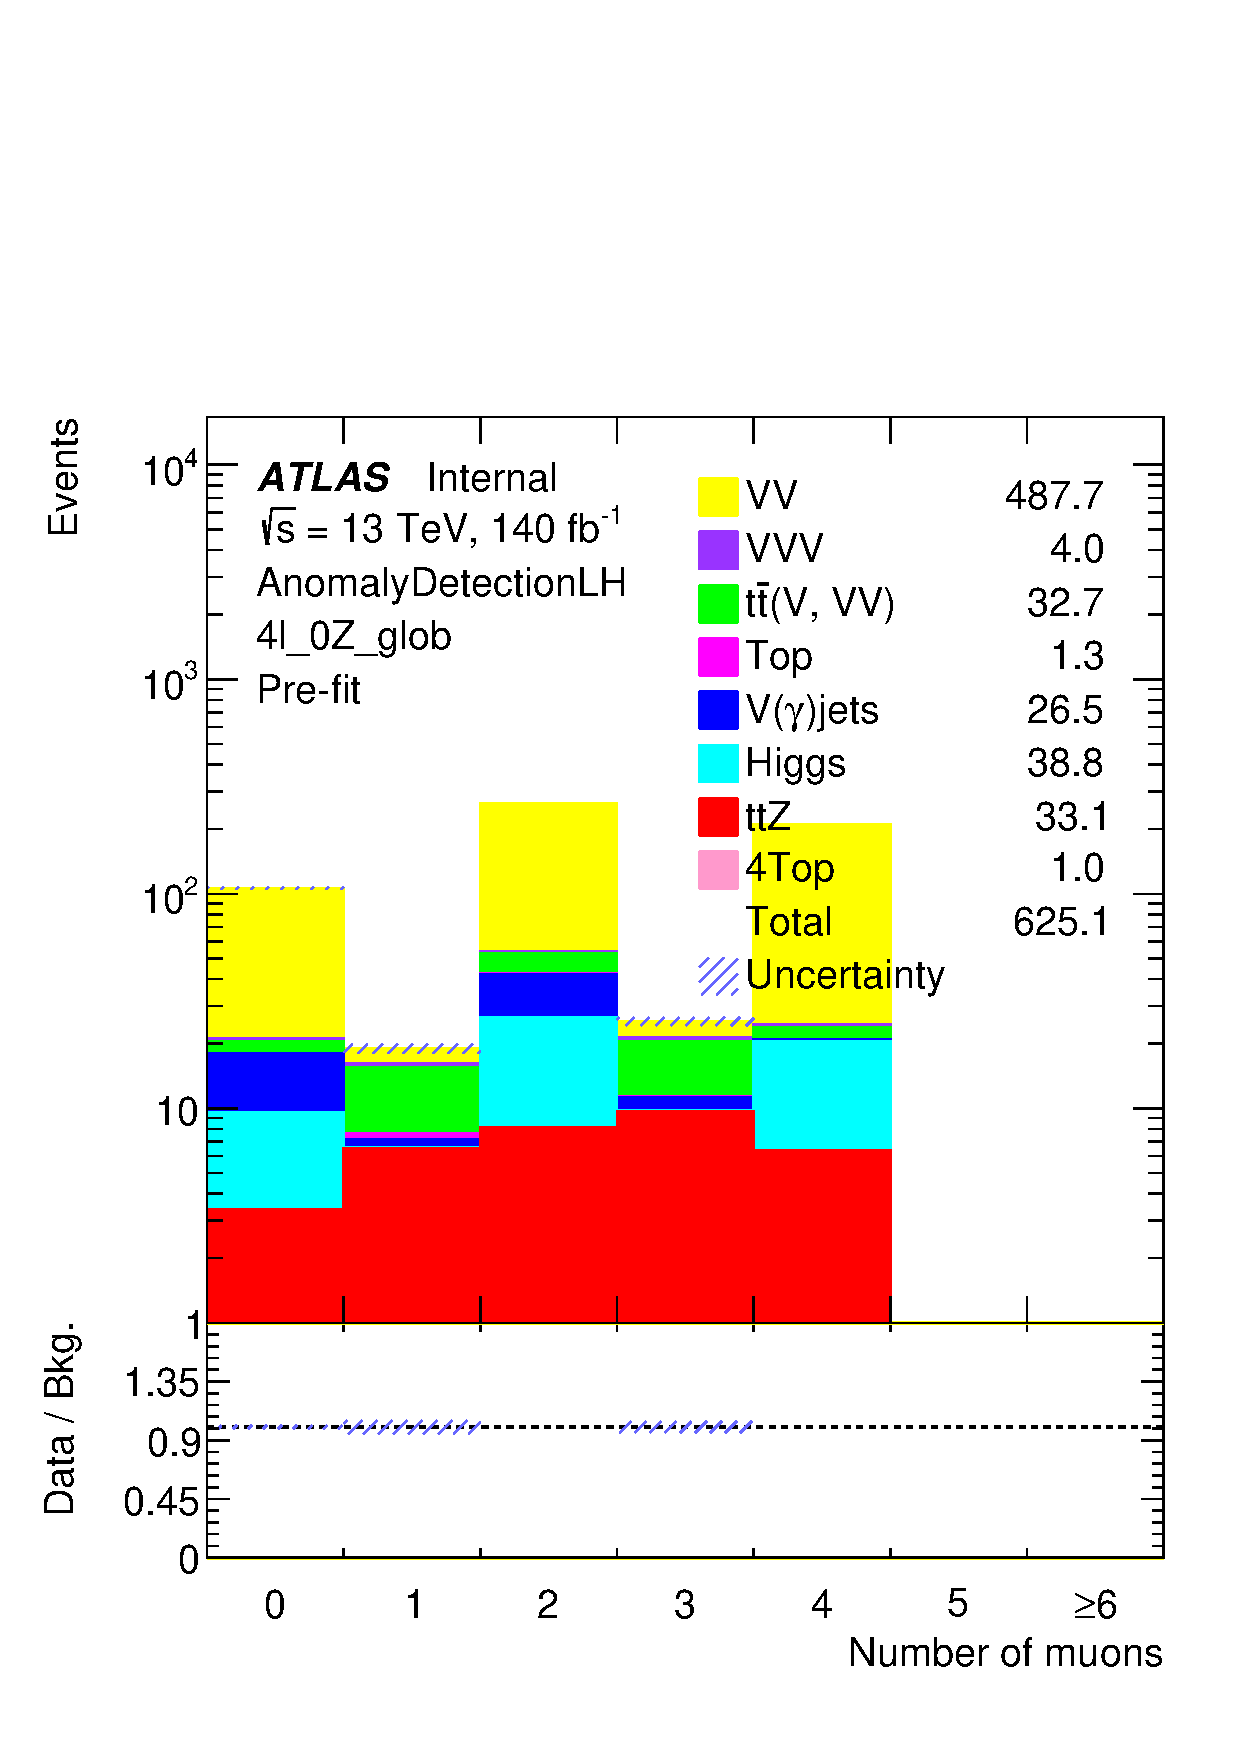
\includegraphics[width=0.24\textwidth]{plots/fourlepLH_run2/Plots/reg_4l_0Z_glob_nMuons.pdf} \\

\end{tabular}
\end{frame}

\begin{frame}{\texttt{Results: 4l\_0Z}}
\begin{tabular}{cccccc}
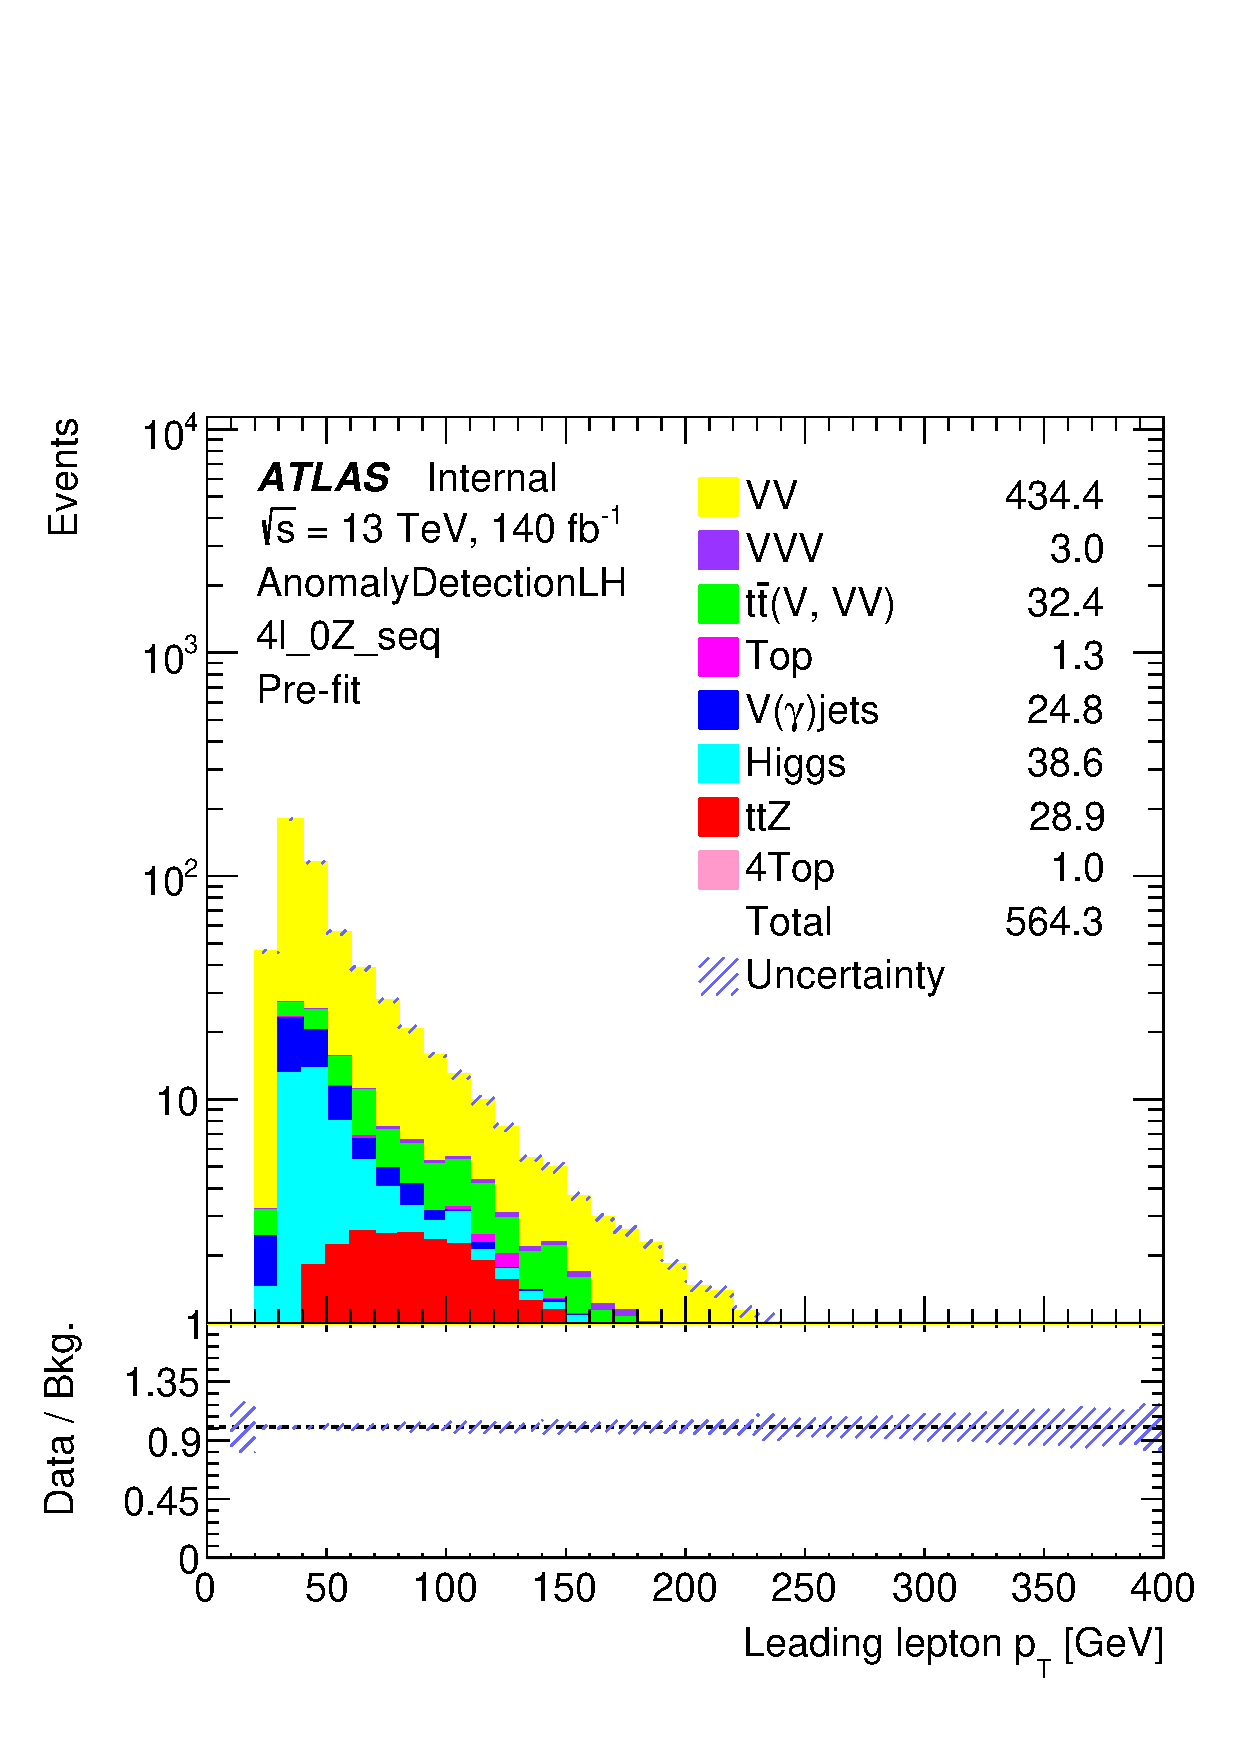
\includegraphics[width=0.24\textwidth]{plots/fourlepLH_run2/Plots/reg_4l_0Z_seq_lep_pt_0.pdf} &
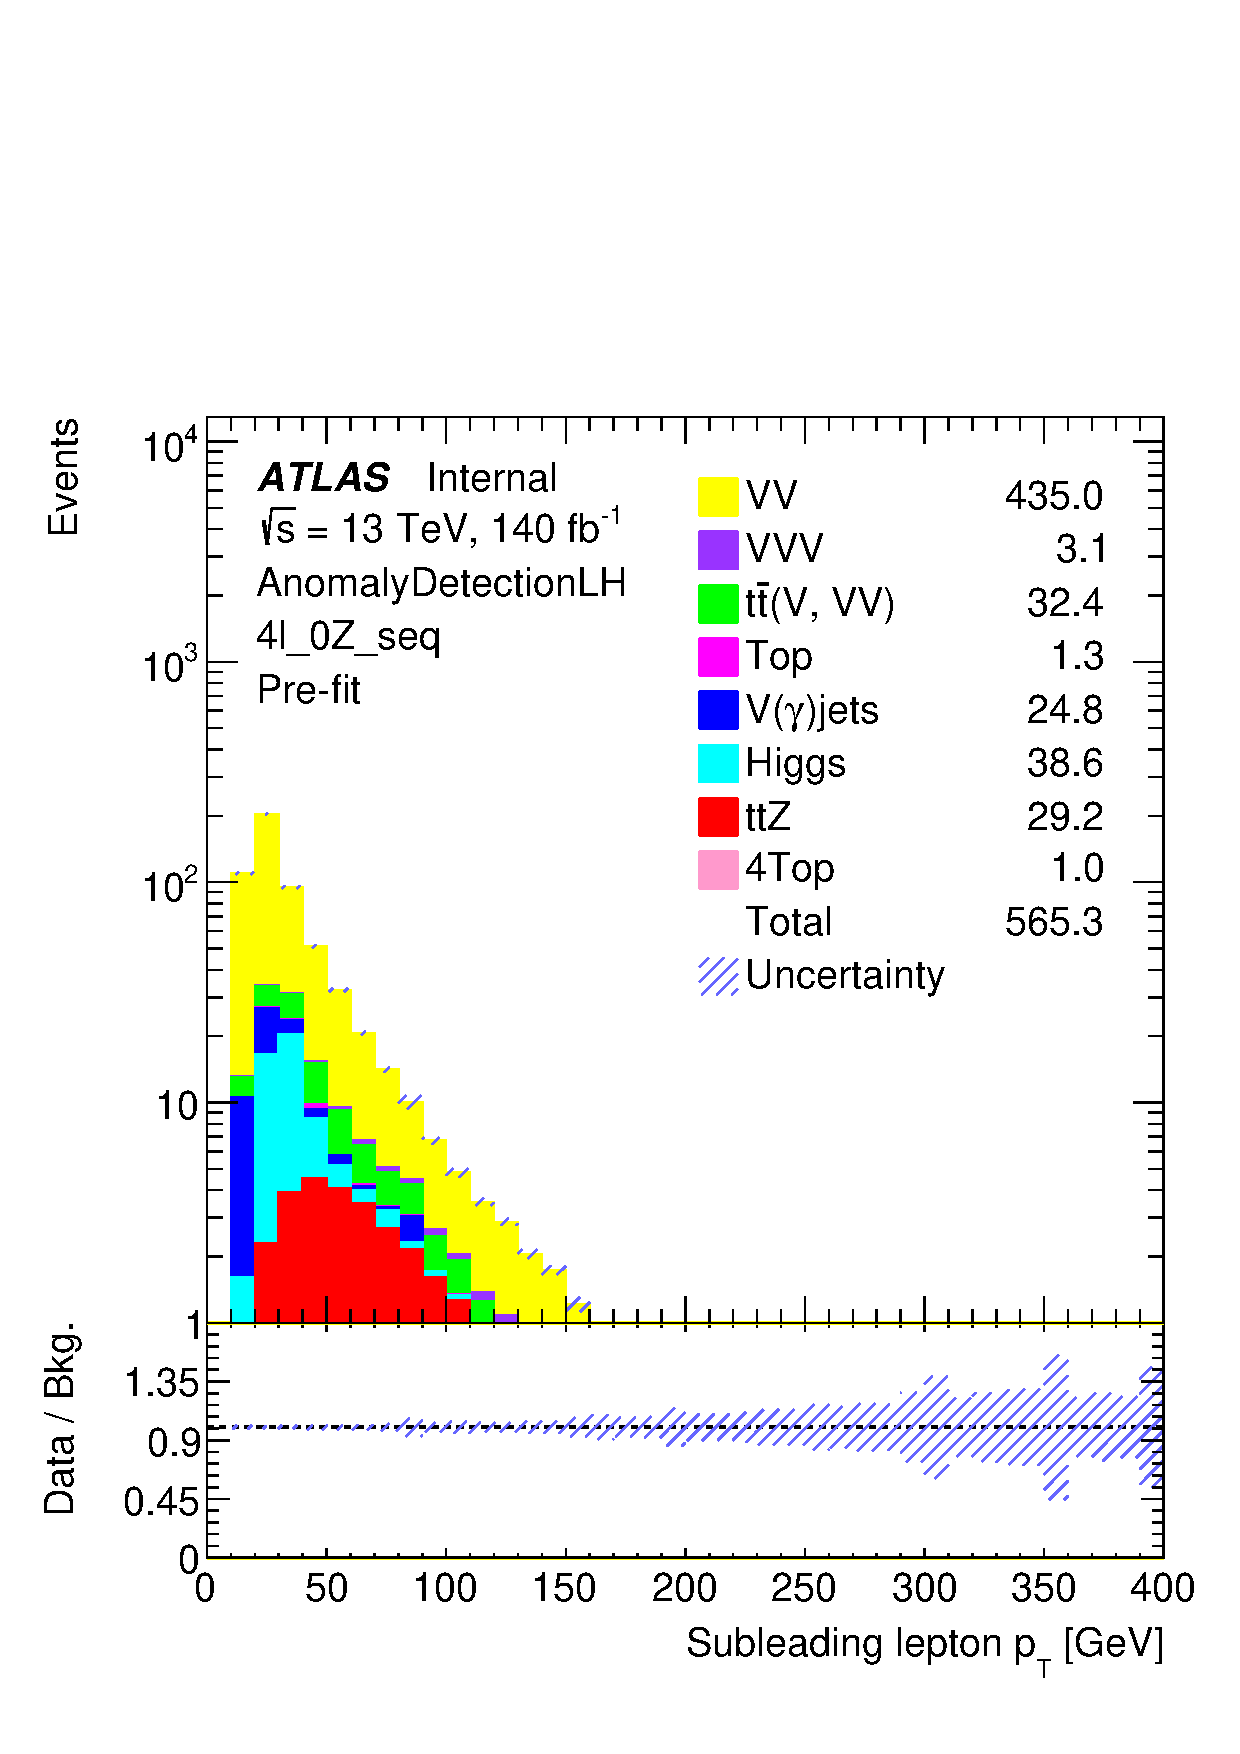
\includegraphics[width=0.24\textwidth]{plots/fourlepLH_run2/Plots/reg_4l_0Z_seq_lep_pt_1.pdf} &
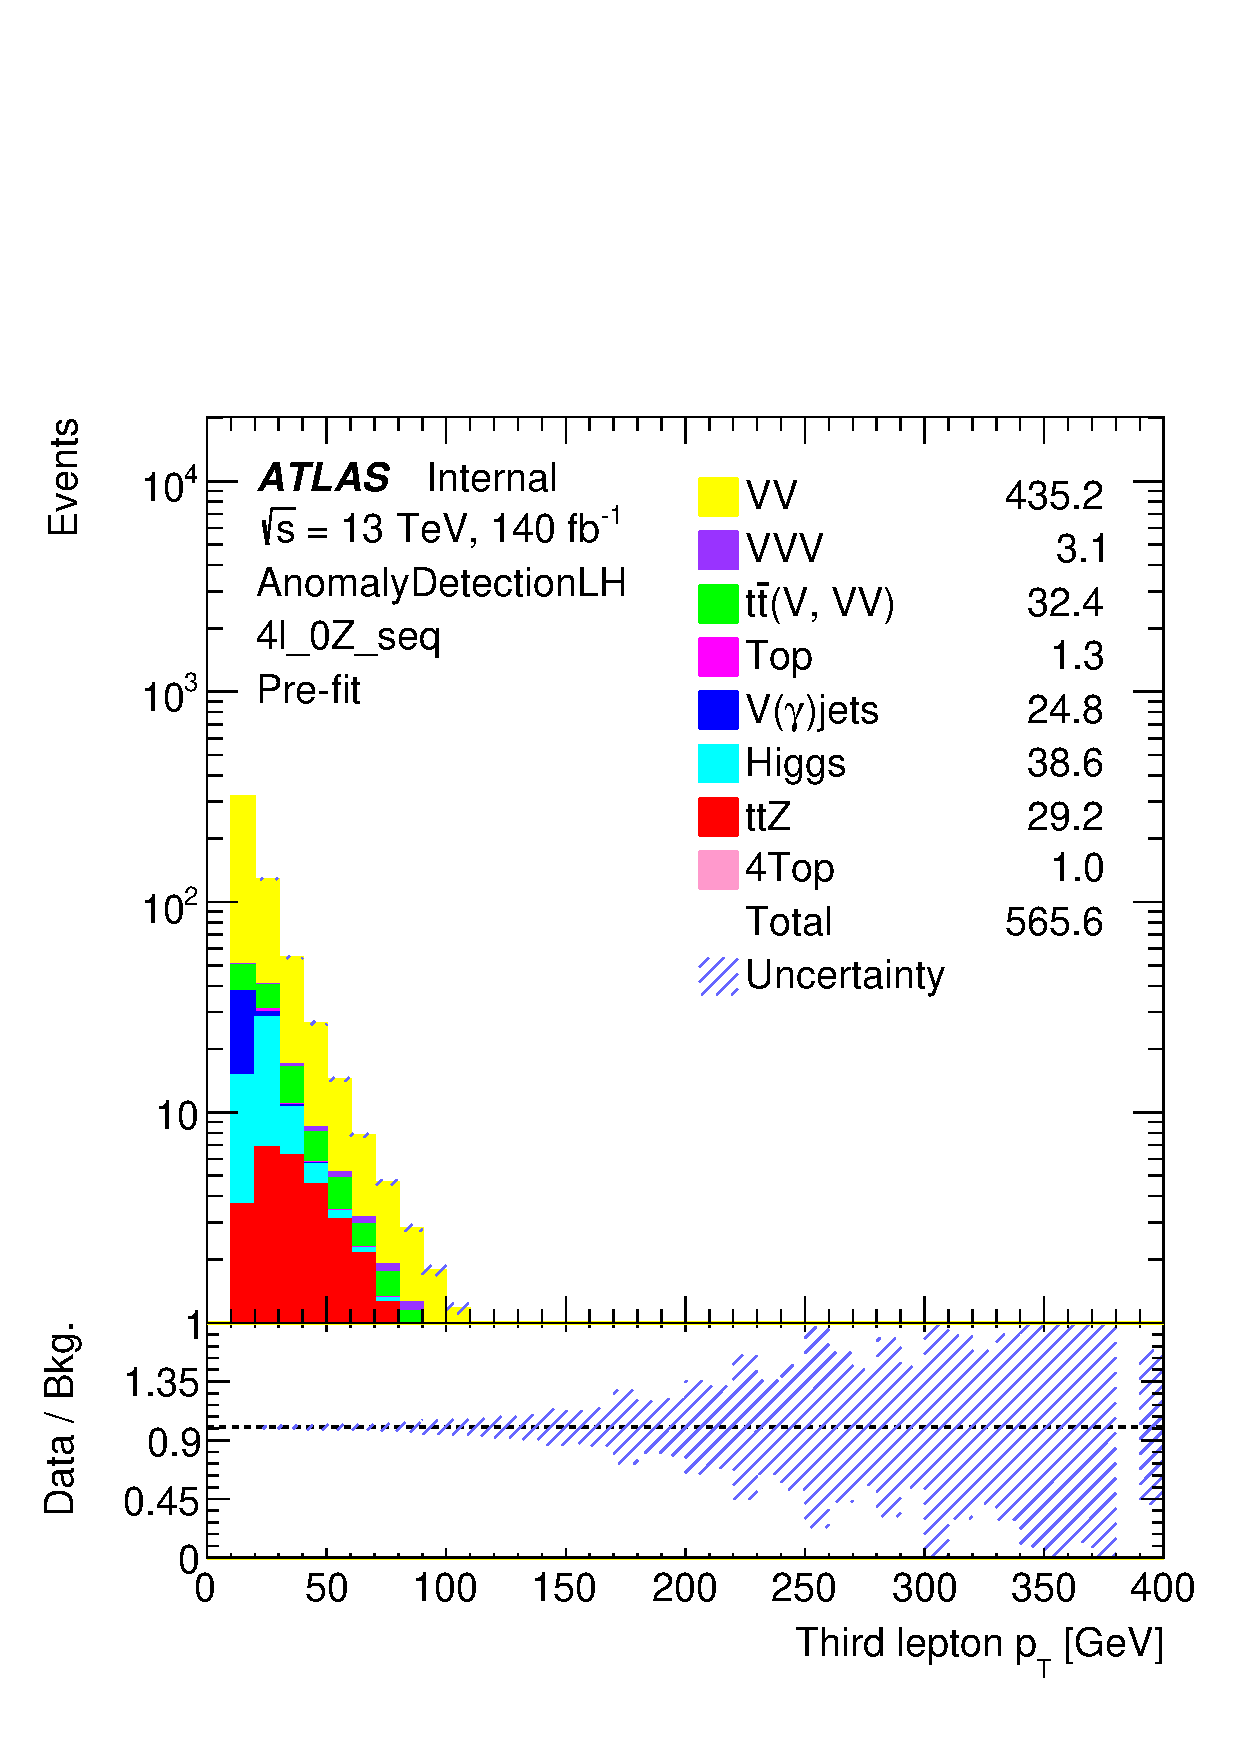
\includegraphics[width=0.24\textwidth]{plots/fourlepLH_run2/Plots/reg_4l_0Z_seq_lep_pt_2.pdf} &
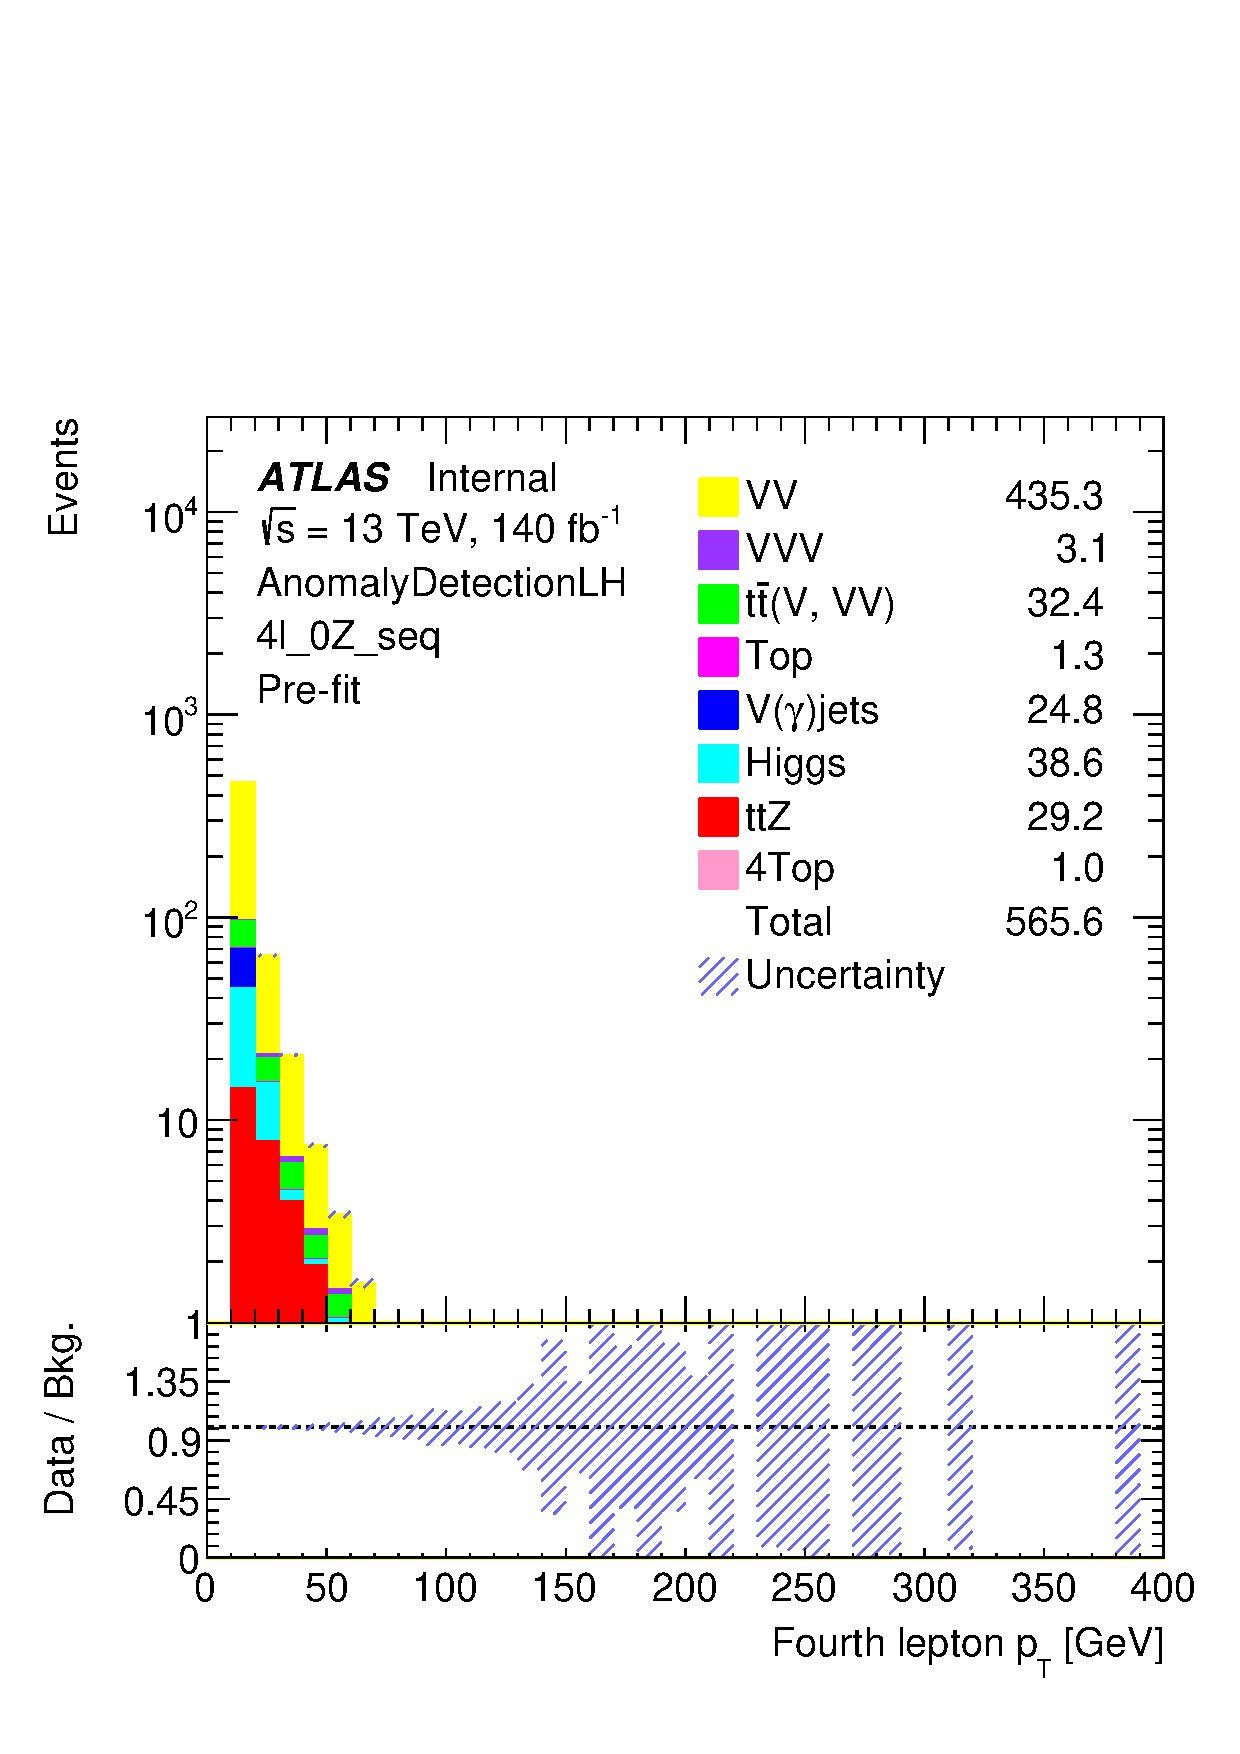
\includegraphics[width=0.24\textwidth]{plots/fourlepLH_run2/Plots/reg_4l_0Z_seq_lep_pt_3.pdf} \\

\includegraphics[width=0.24\textwidth]{plots/fourlepLH_run2/Plots/reg_4l_0Z_glob_lep_pt_0.pdf} &
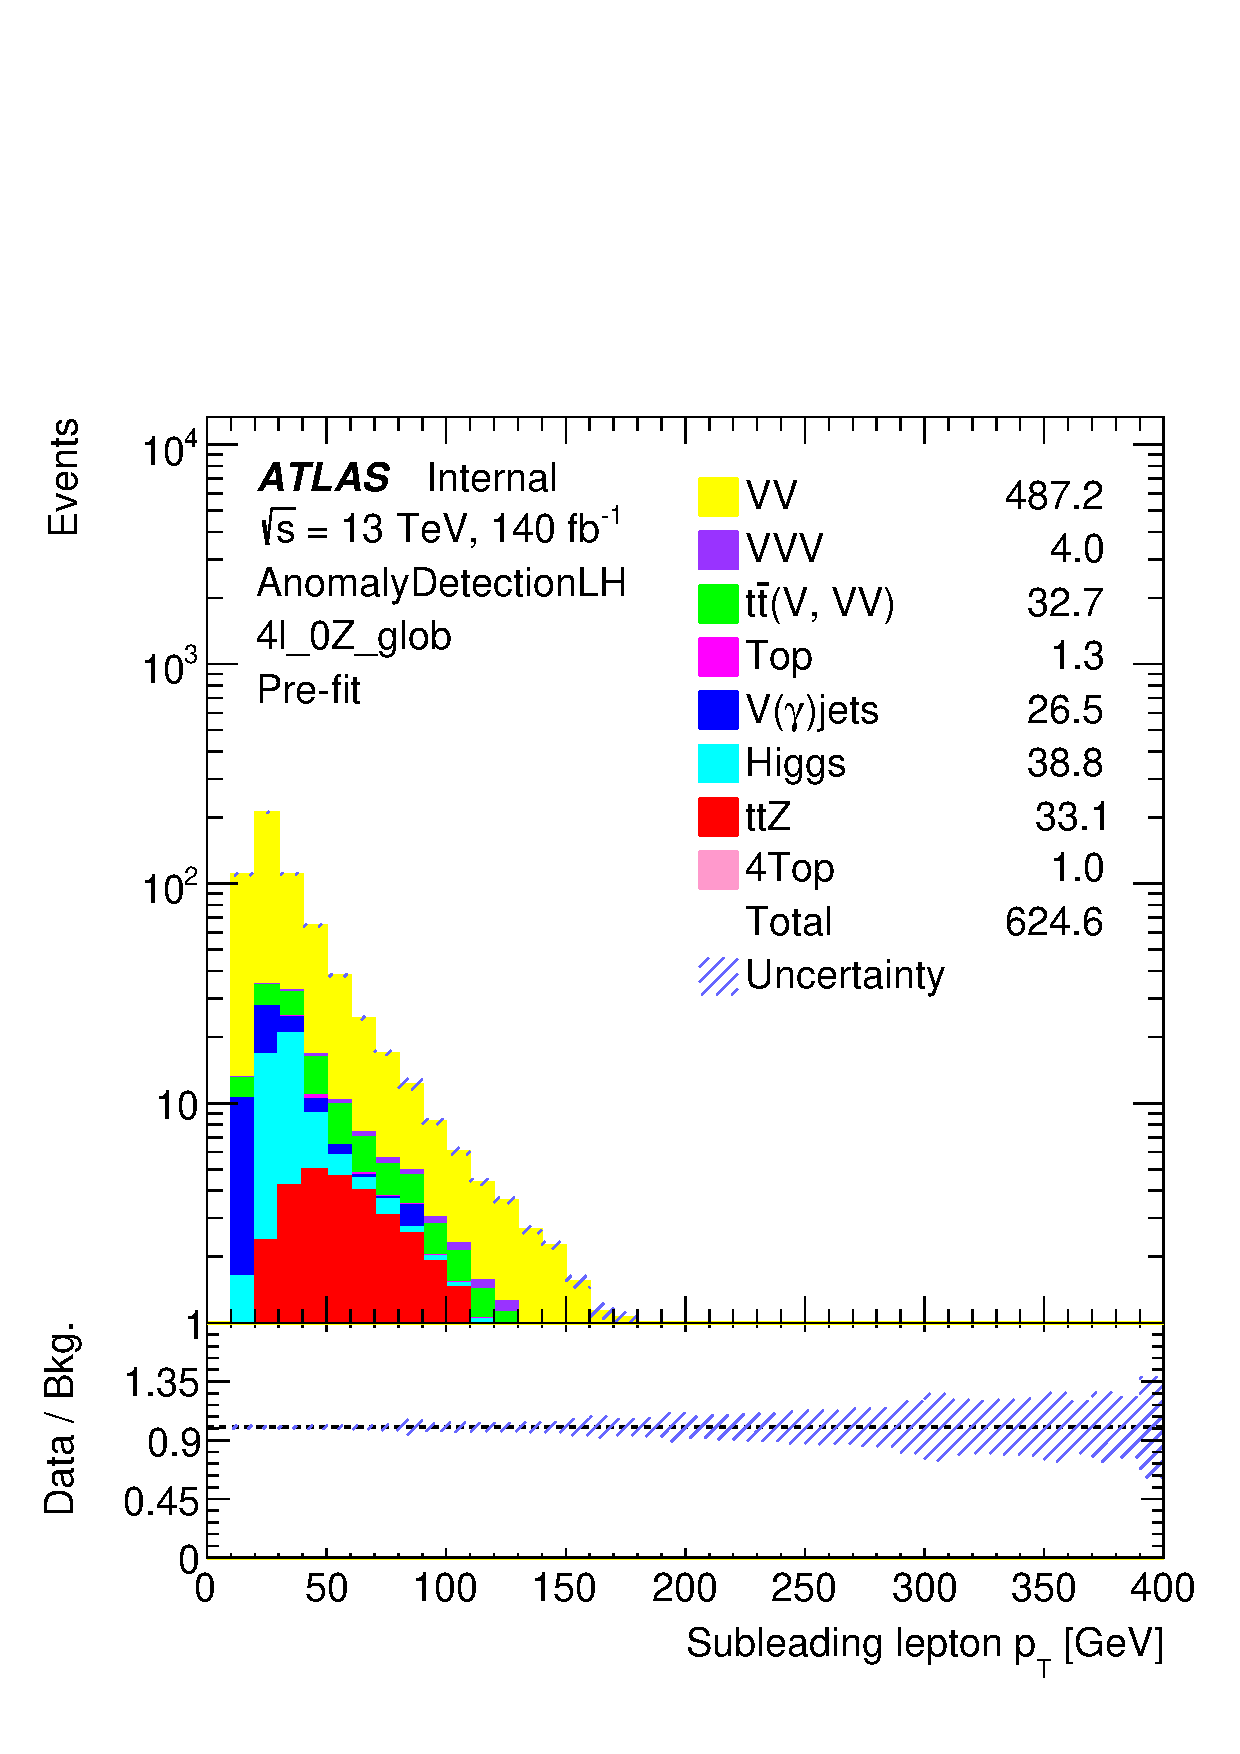
\includegraphics[width=0.24\textwidth]{plots/fourlepLH_run2/Plots/reg_4l_0Z_glob_lep_pt_1.pdf} &
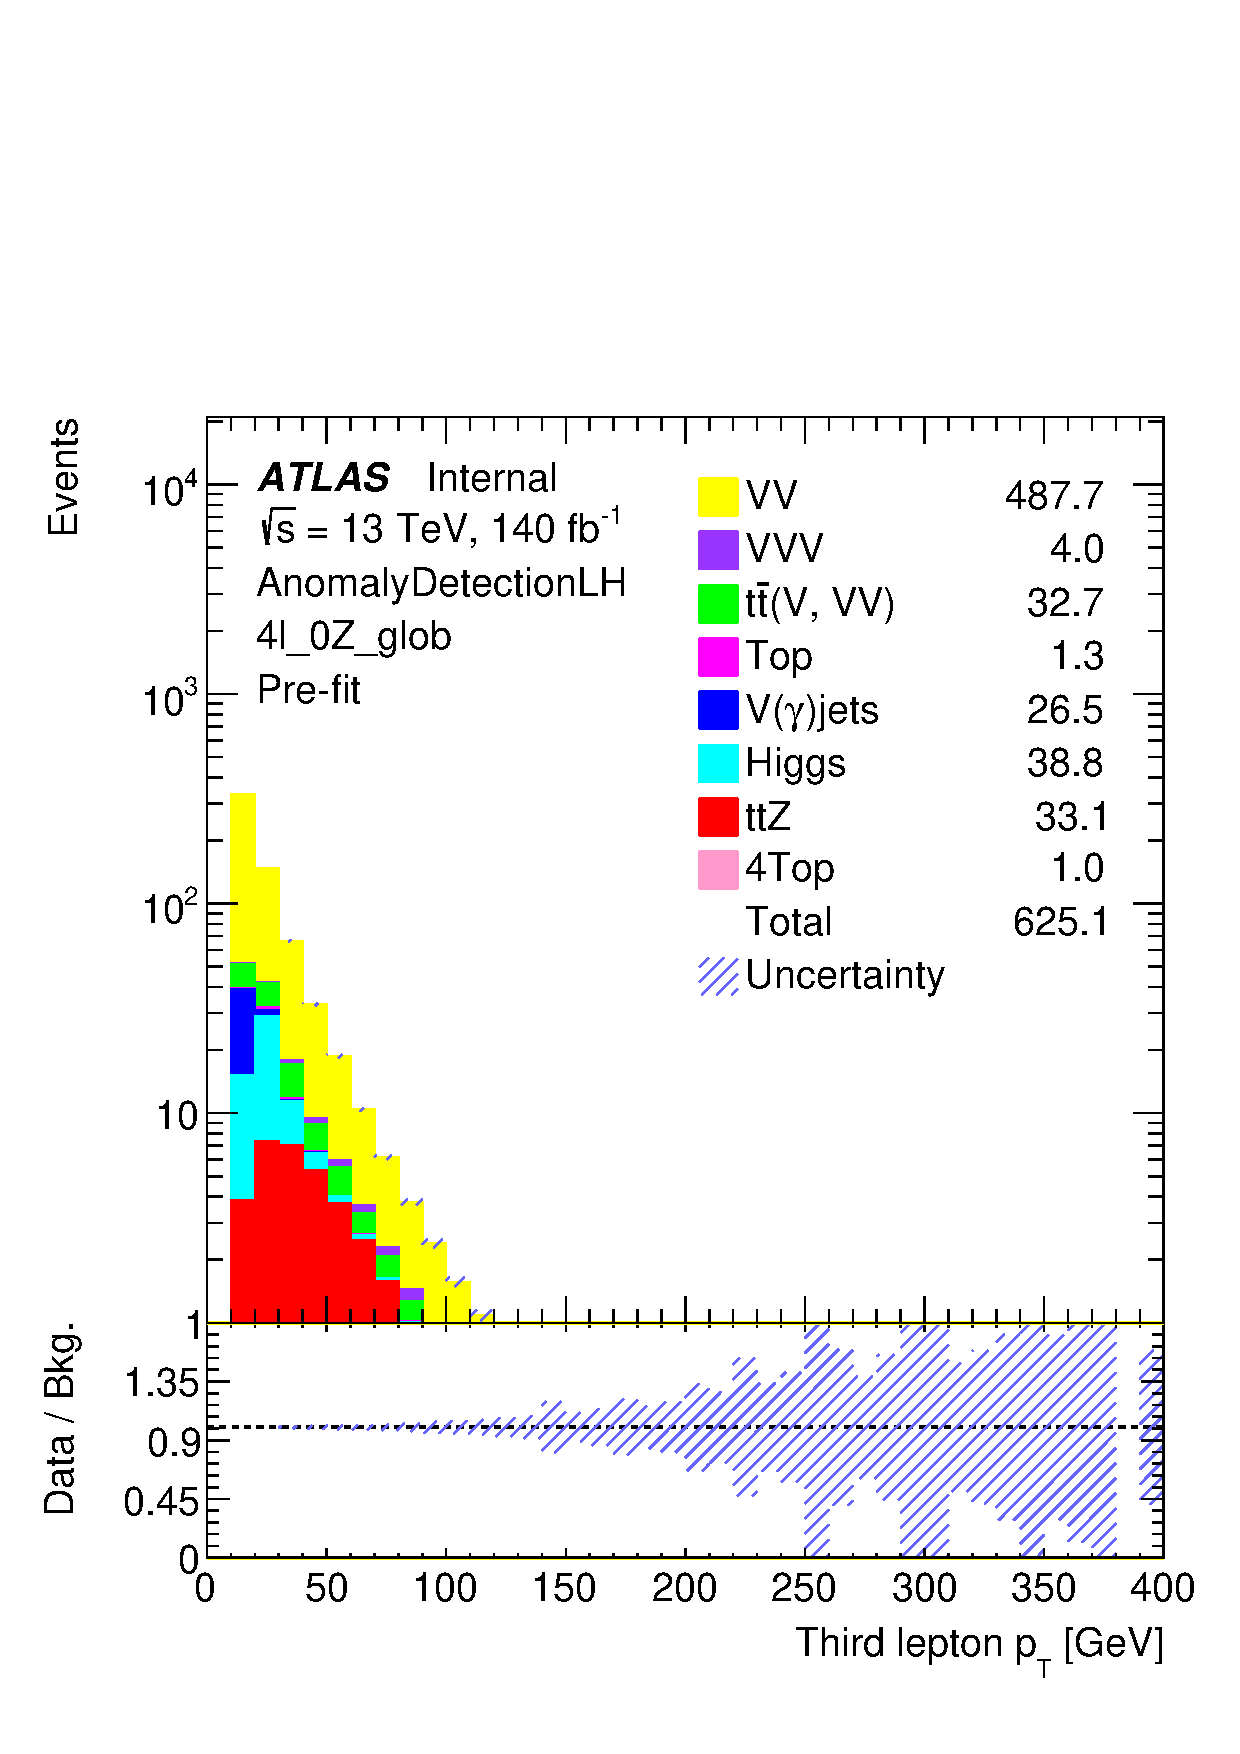
\includegraphics[width=0.24\textwidth]{plots/fourlepLH_run2/Plots/reg_4l_0Z_glob_lep_pt_2.pdf} &
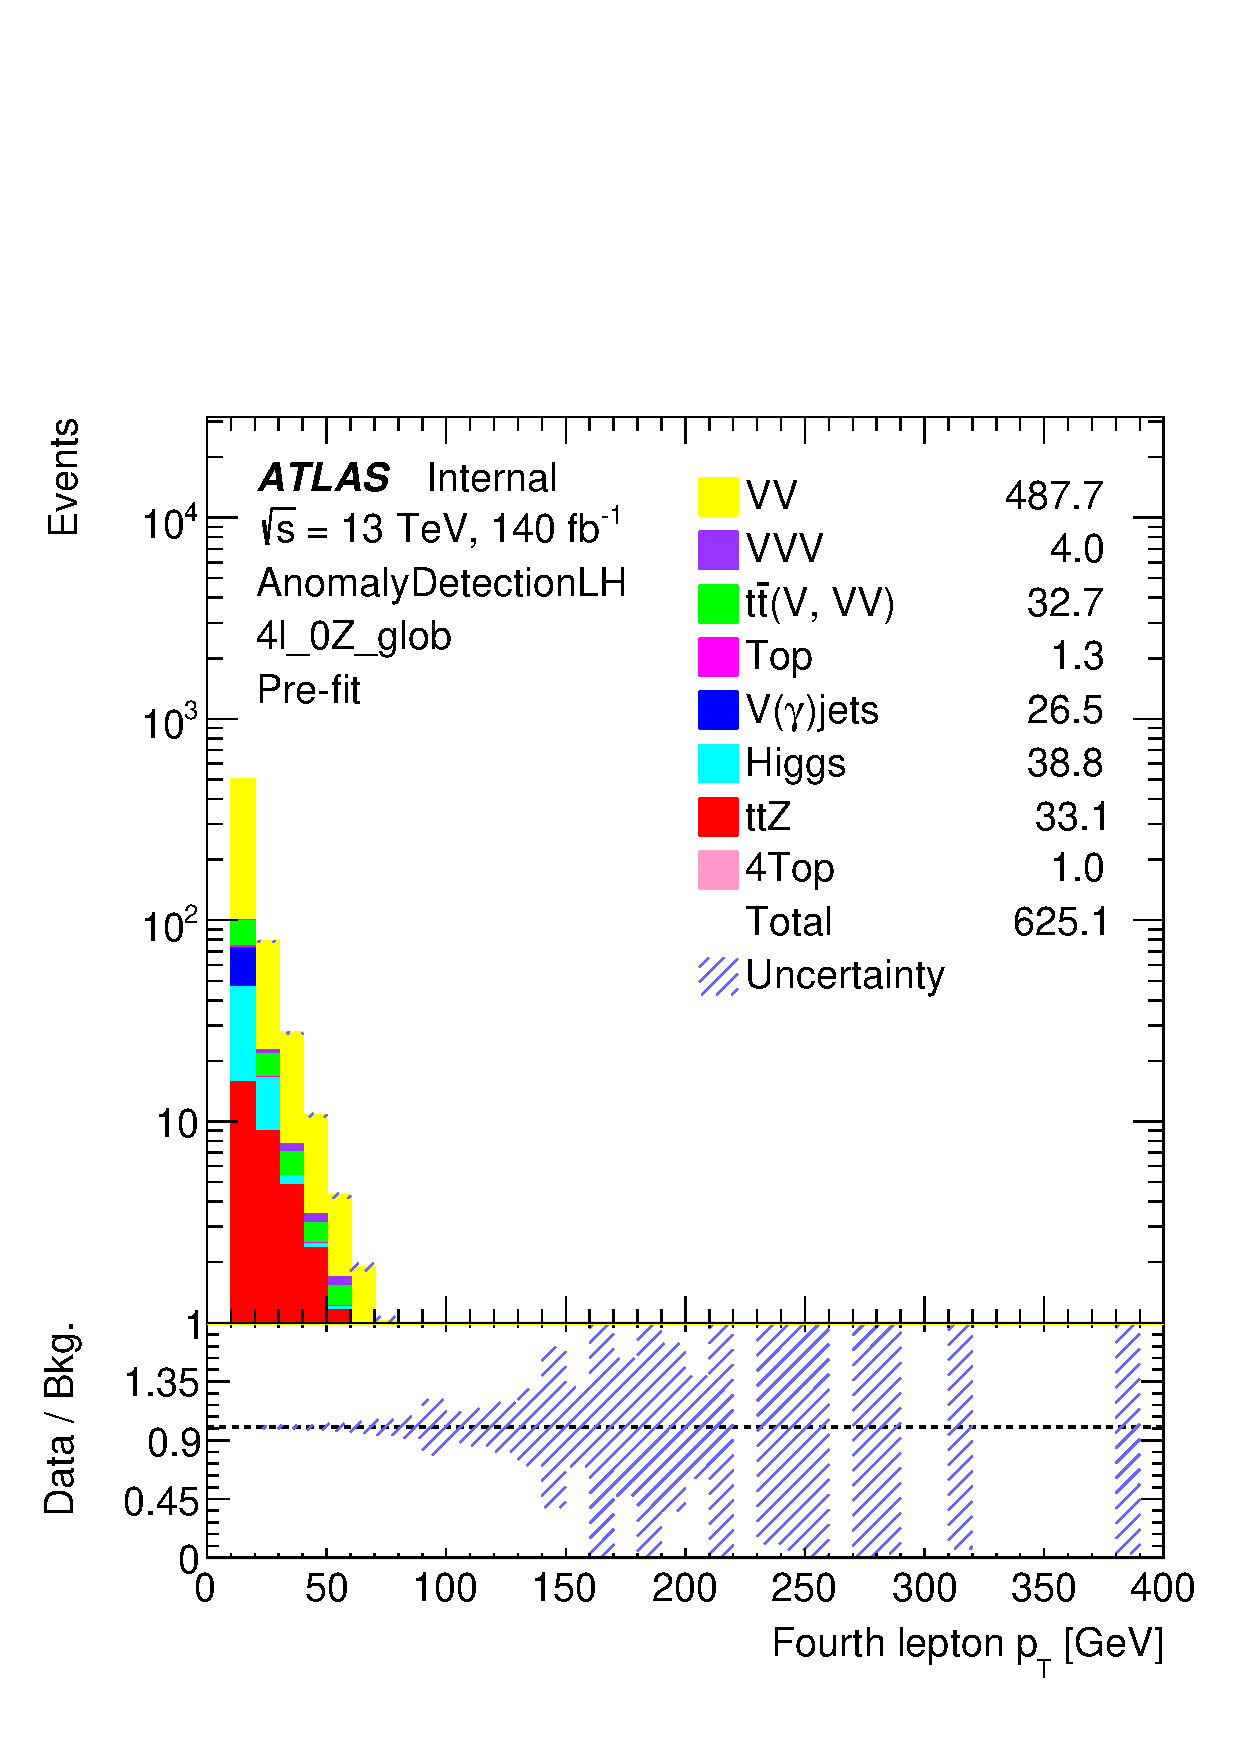
\includegraphics[width=0.24\textwidth]{plots/fourlepLH_run2/Plots/reg_4l_0Z_glob_lep_pt_3.pdf} \\

\end{tabular}

\end{frame}
\subsection{4l\_0Z\_0b}
\begin{frame}{\texttt{Focused selection: 4l\_0Z\_0b}}
%\tiny
\centering
\begin{tabular}{|c|c|}
\hline

4l\_0Z\_0b\_seq &
4l\_0Z\_0b\_glob \\
\hline
\multicolumn{2}{|c|}{\texttt{globalTriggerMatchSLTorDLT\_LooseLH\_custTrig\_NOSYS}} \\
\multicolumn{2}{|c|}{\texttt{pass\_fourlep\_LooseLH\_NOSYS} }\\
\multicolumn{2}{|c|}{\texttt{$N_{leptons}$=4}} \\
\multicolumn{2}{|c|}{\texttt{$N_{taus}$ $\geq 0$} } \\
\multicolumn{2}{|c|}{$N_{b\mathrm{-jets}}$ $= 0$} \\
\multicolumn{2}{|c|}{\texttt{Q = 0}} \\

\hline

\texttt{$|m_{Z1}^{seq}-91.2e3| < 10e3$} &
\texttt{$|m_{Z1}^{glob}-91.2e3| < 10e3$} &\\
\texttt{$|m_{Z2}^{seq}-91.2e3| < 10e3$} &
\texttt{$|m_{Z2}^{glob}-91.2e3| < 10e3$}\\

\hline

\end{tabular}
\end{frame}

\begin{frame}{\texttt{Results: 4l\_0Z\_0b}}
\centering
\begin{tabular}{cccccc}

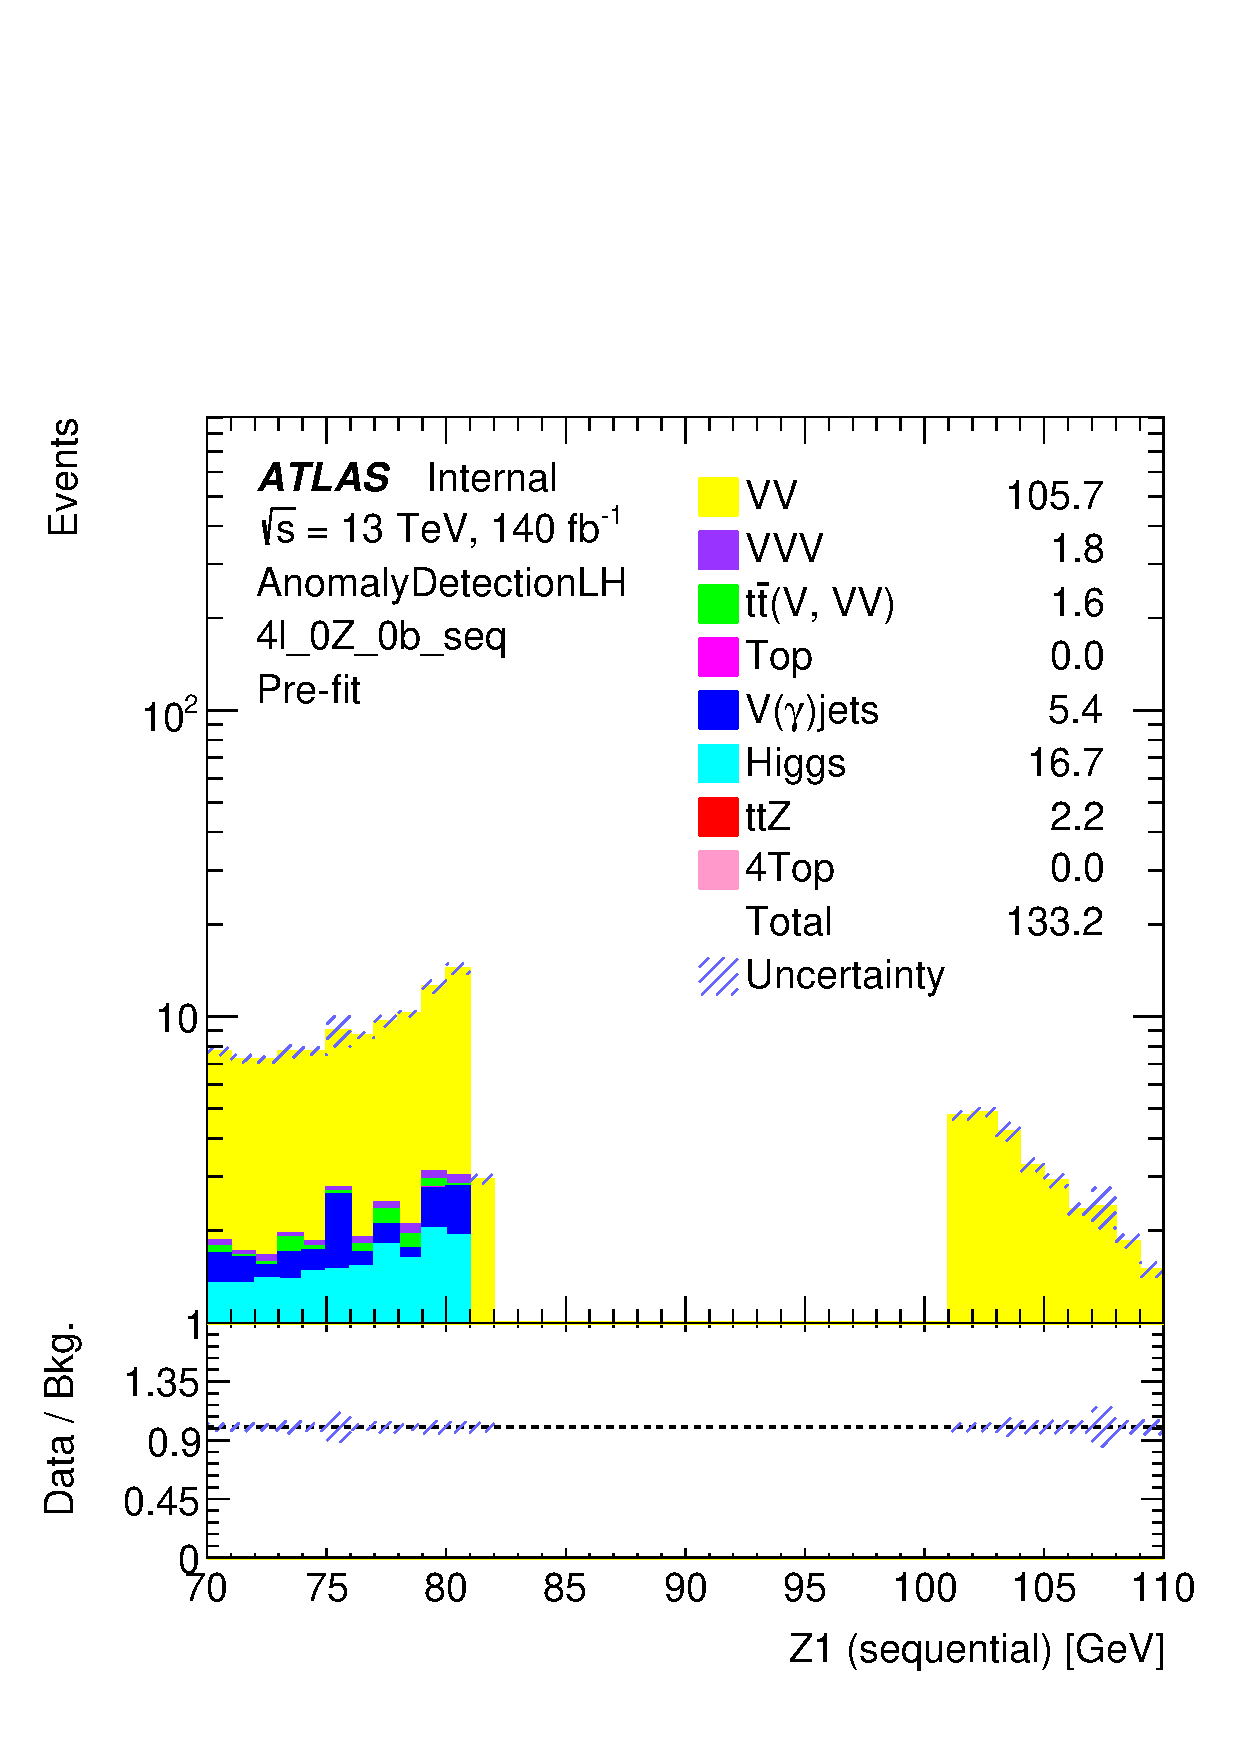
\includegraphics[width=0.24\textwidth]{plots/fourlepLH_run2/Plots/reg_4l_0Z_0b_seq_Z1_mass_seq_1GeV.pdf} &
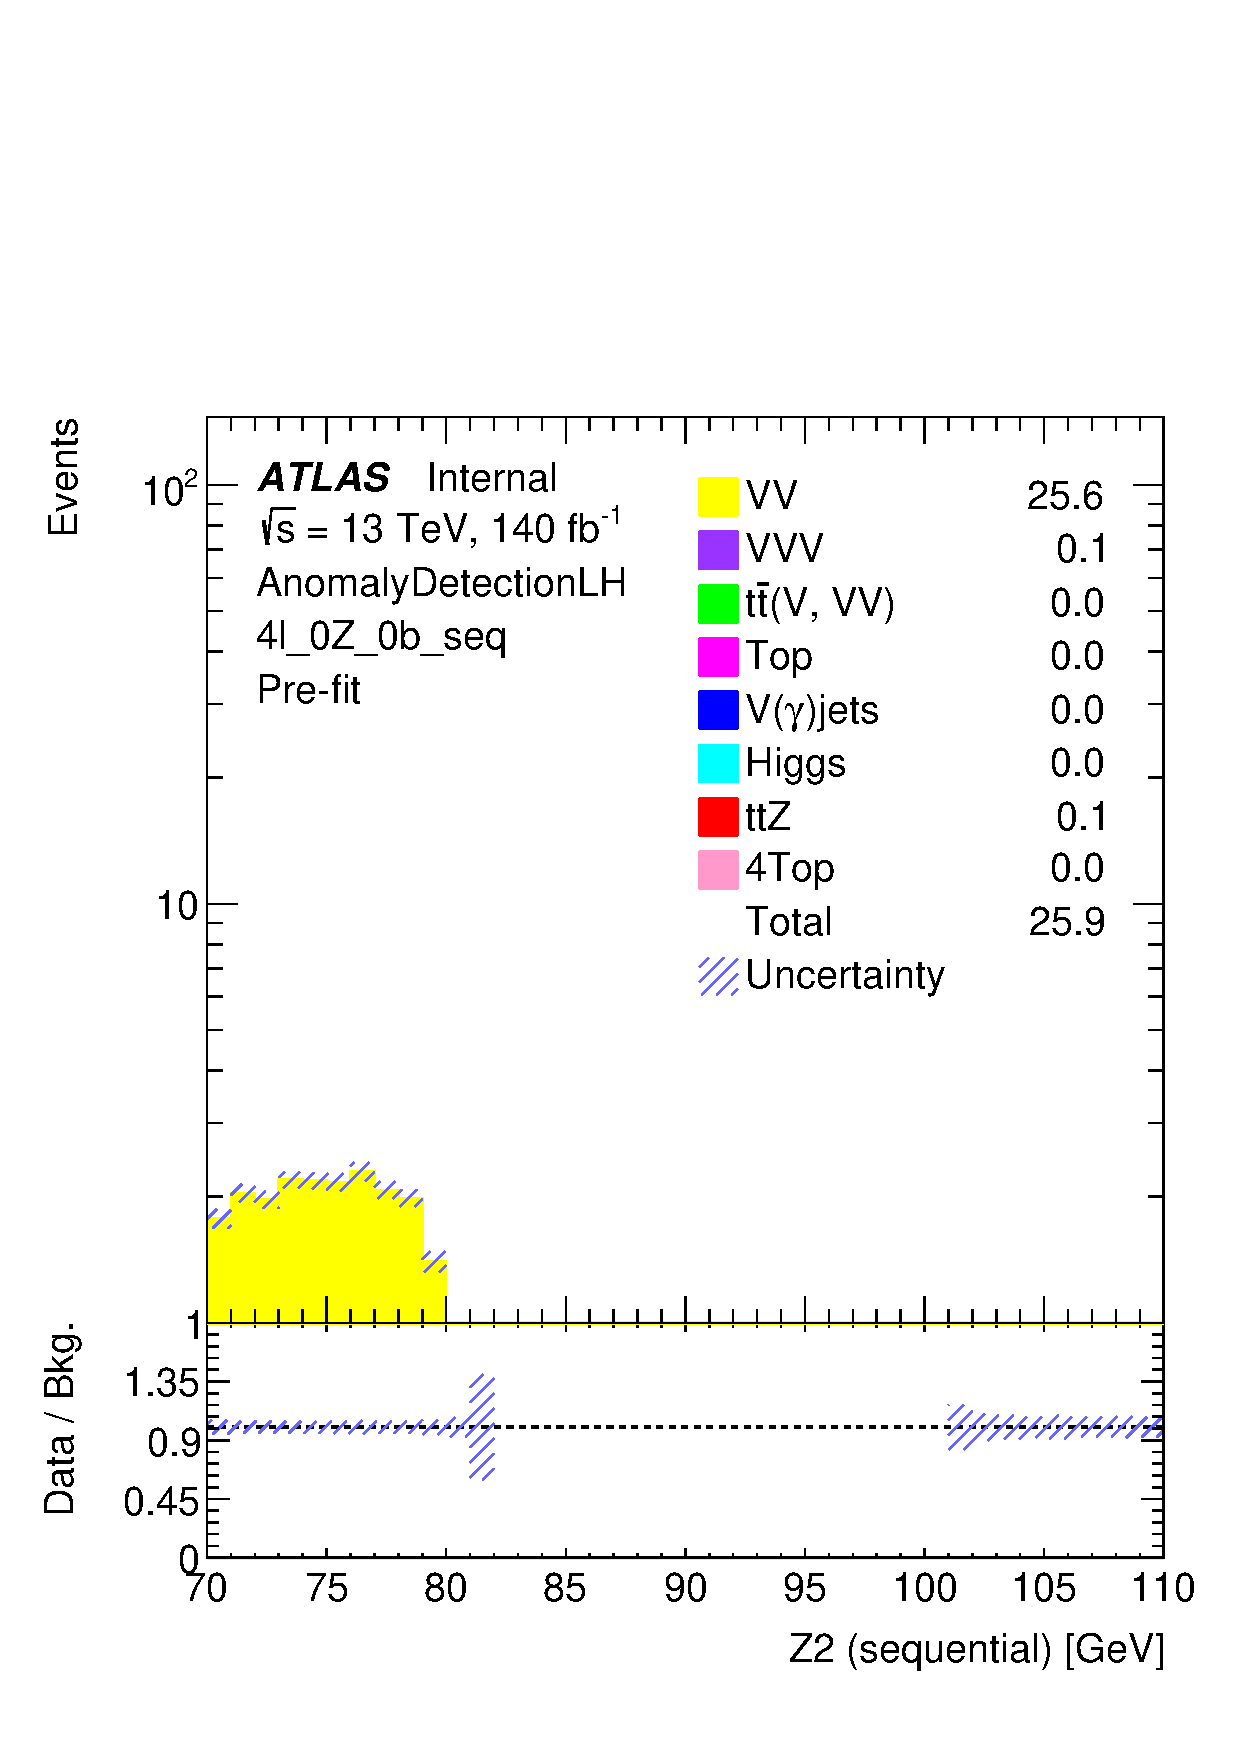
\includegraphics[width=0.24\textwidth]{plots/fourlepLH_run2/Plots/reg_4l_0Z_0b_seq_Z2_mass_seq_1GeV.pdf}  &

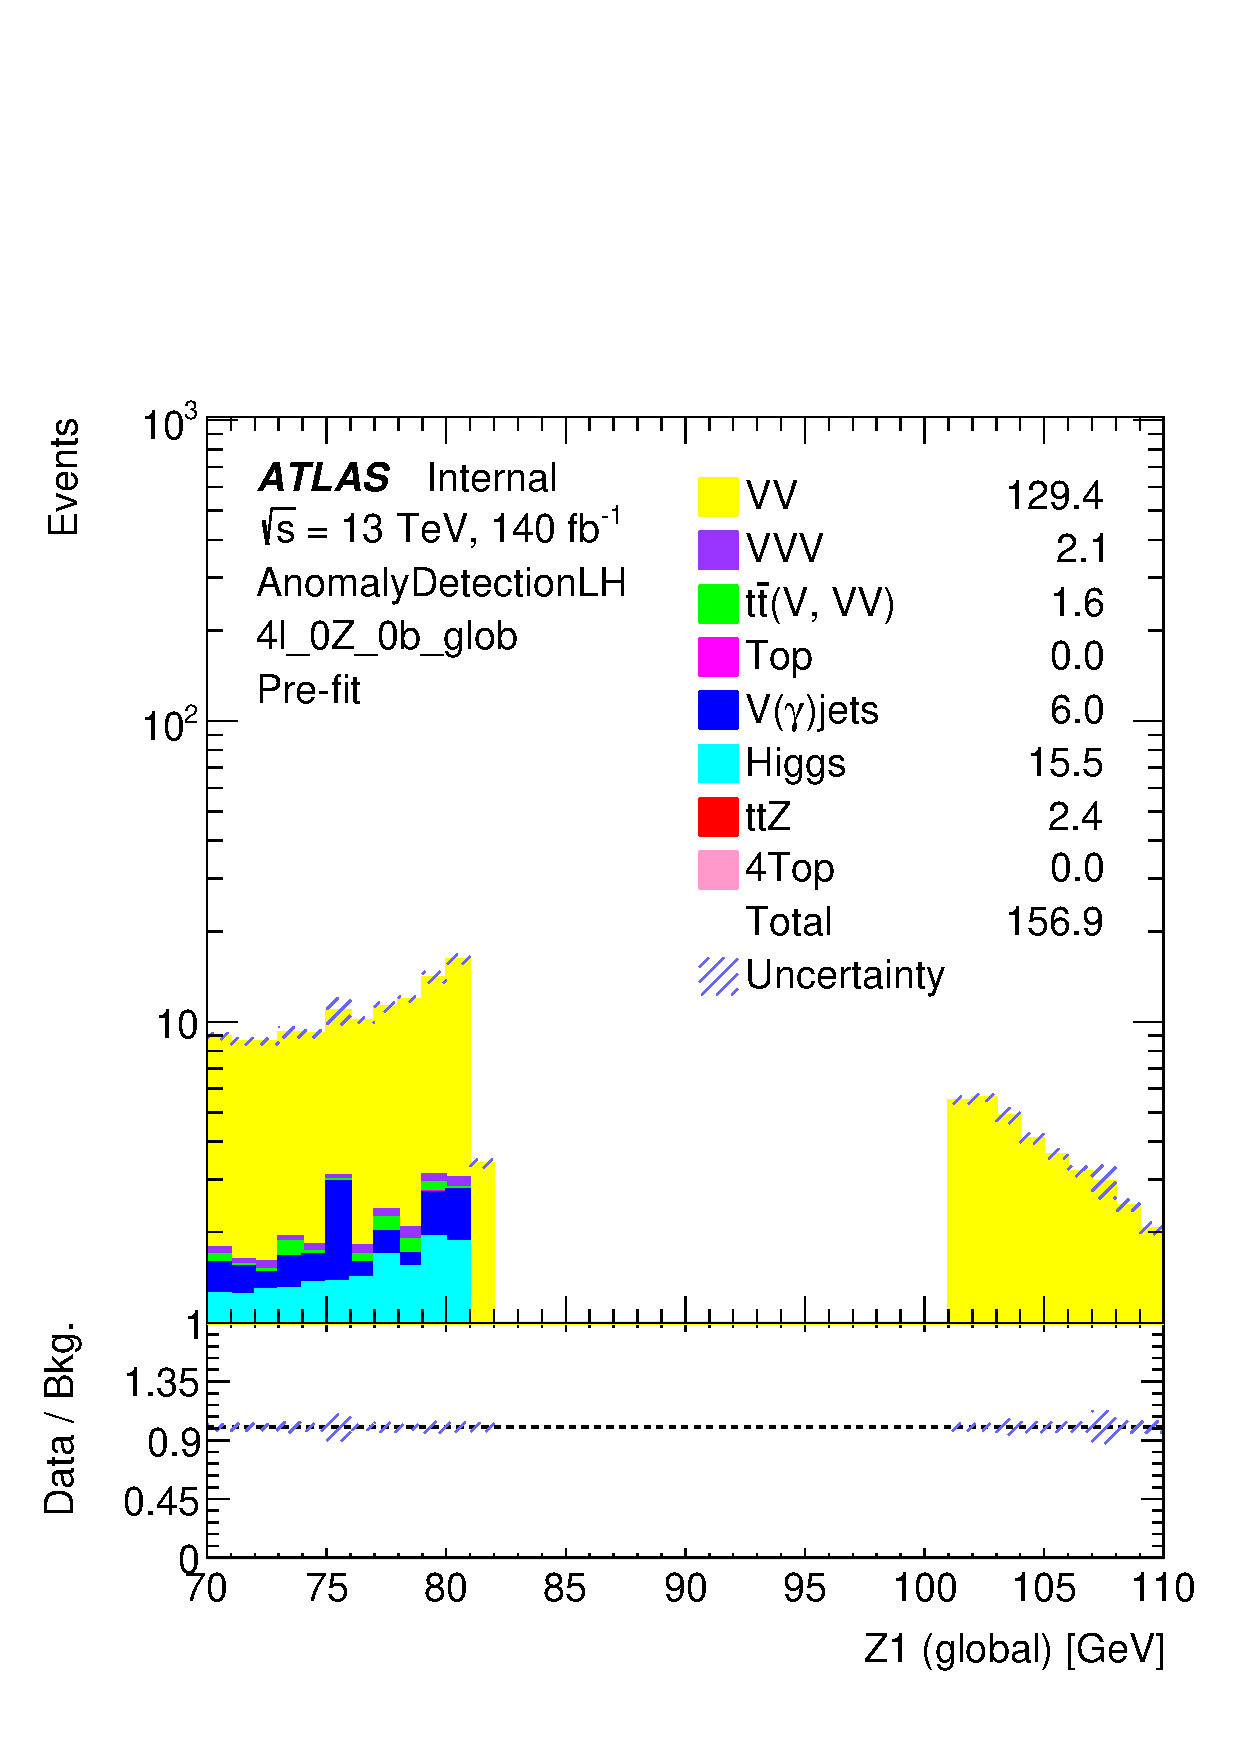
\includegraphics[width=0.24\textwidth]{plots/fourlepLH_run2/Plots/reg_4l_0Z_0b_glob_Z1_mass_glob_1GeV.pdf} &
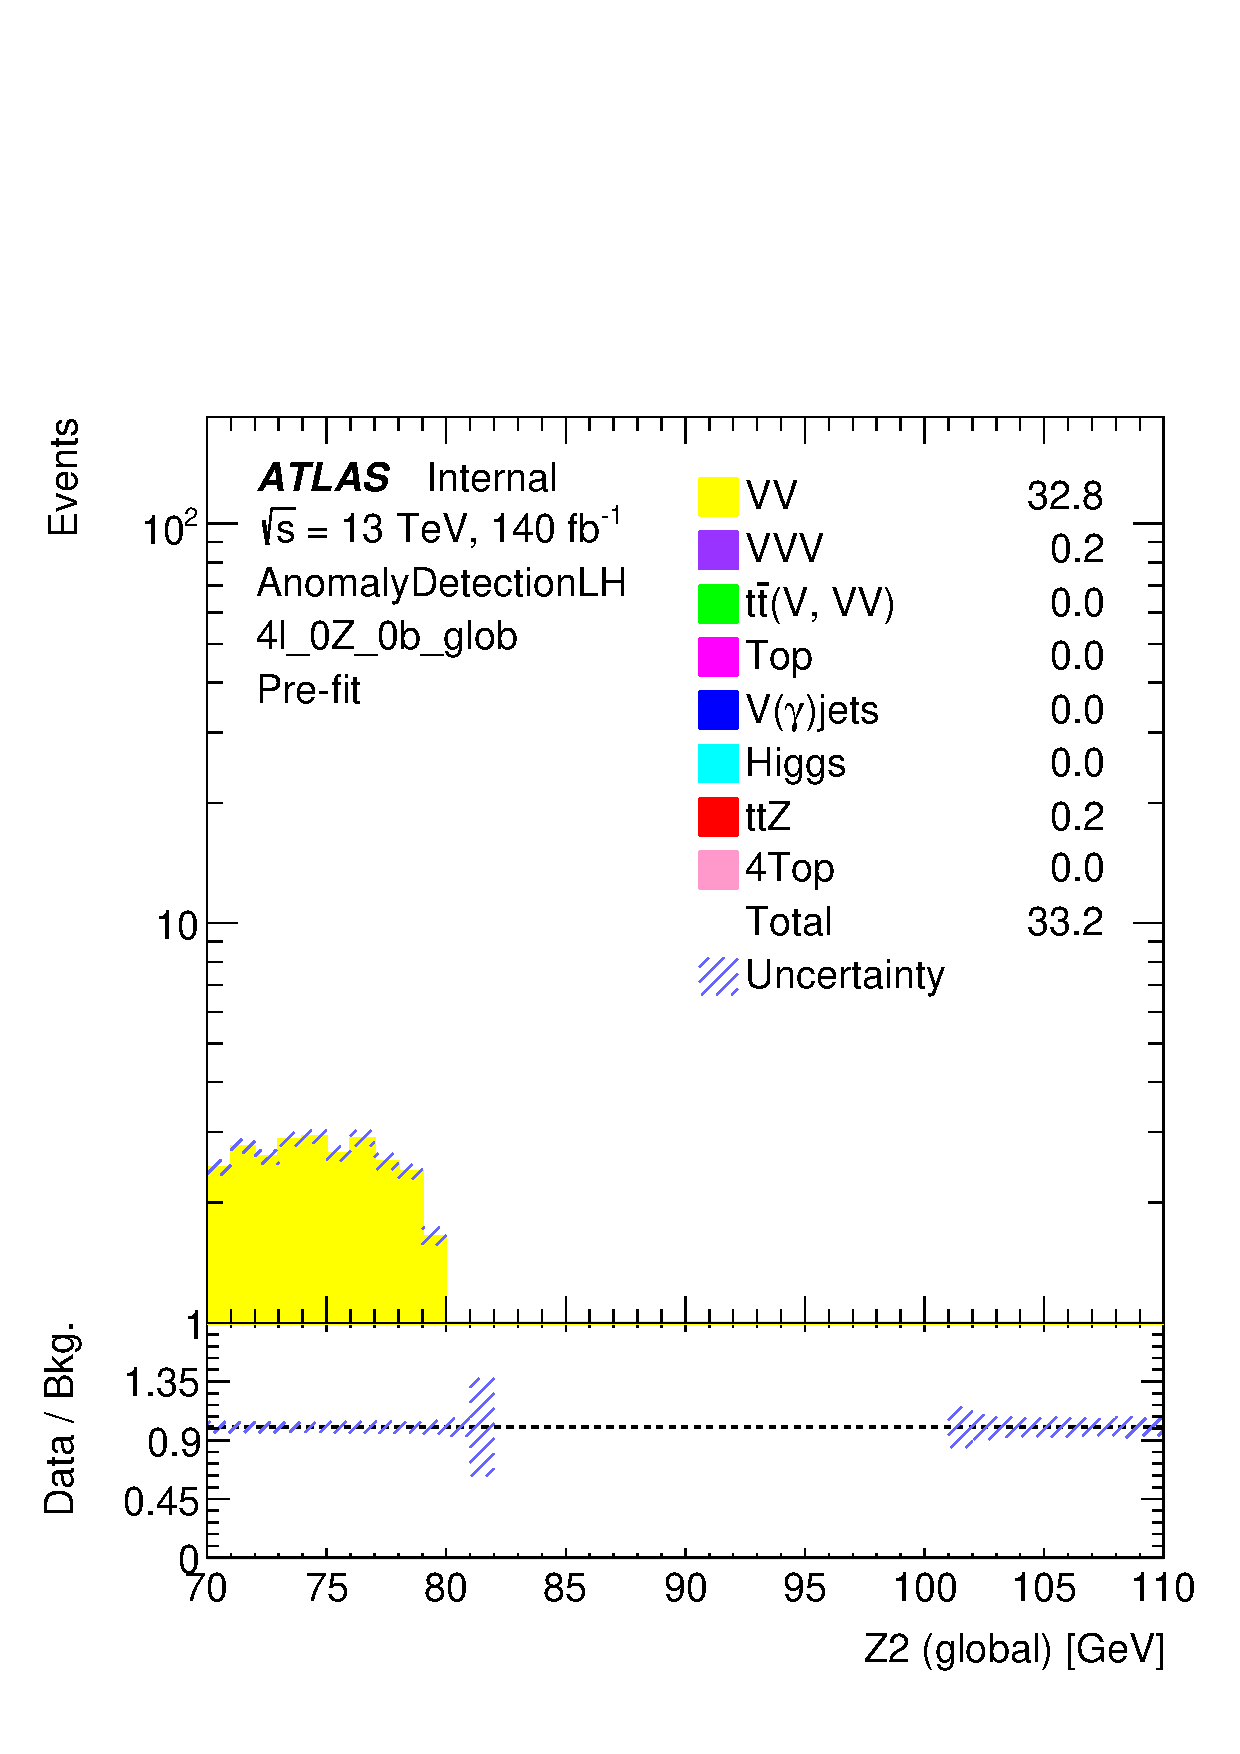
\includegraphics[width=0.24\textwidth]{plots/fourlepLH_run2/Plots/reg_4l_0Z_0b_glob_Z2_mass_glob_1GeV.pdf}\\

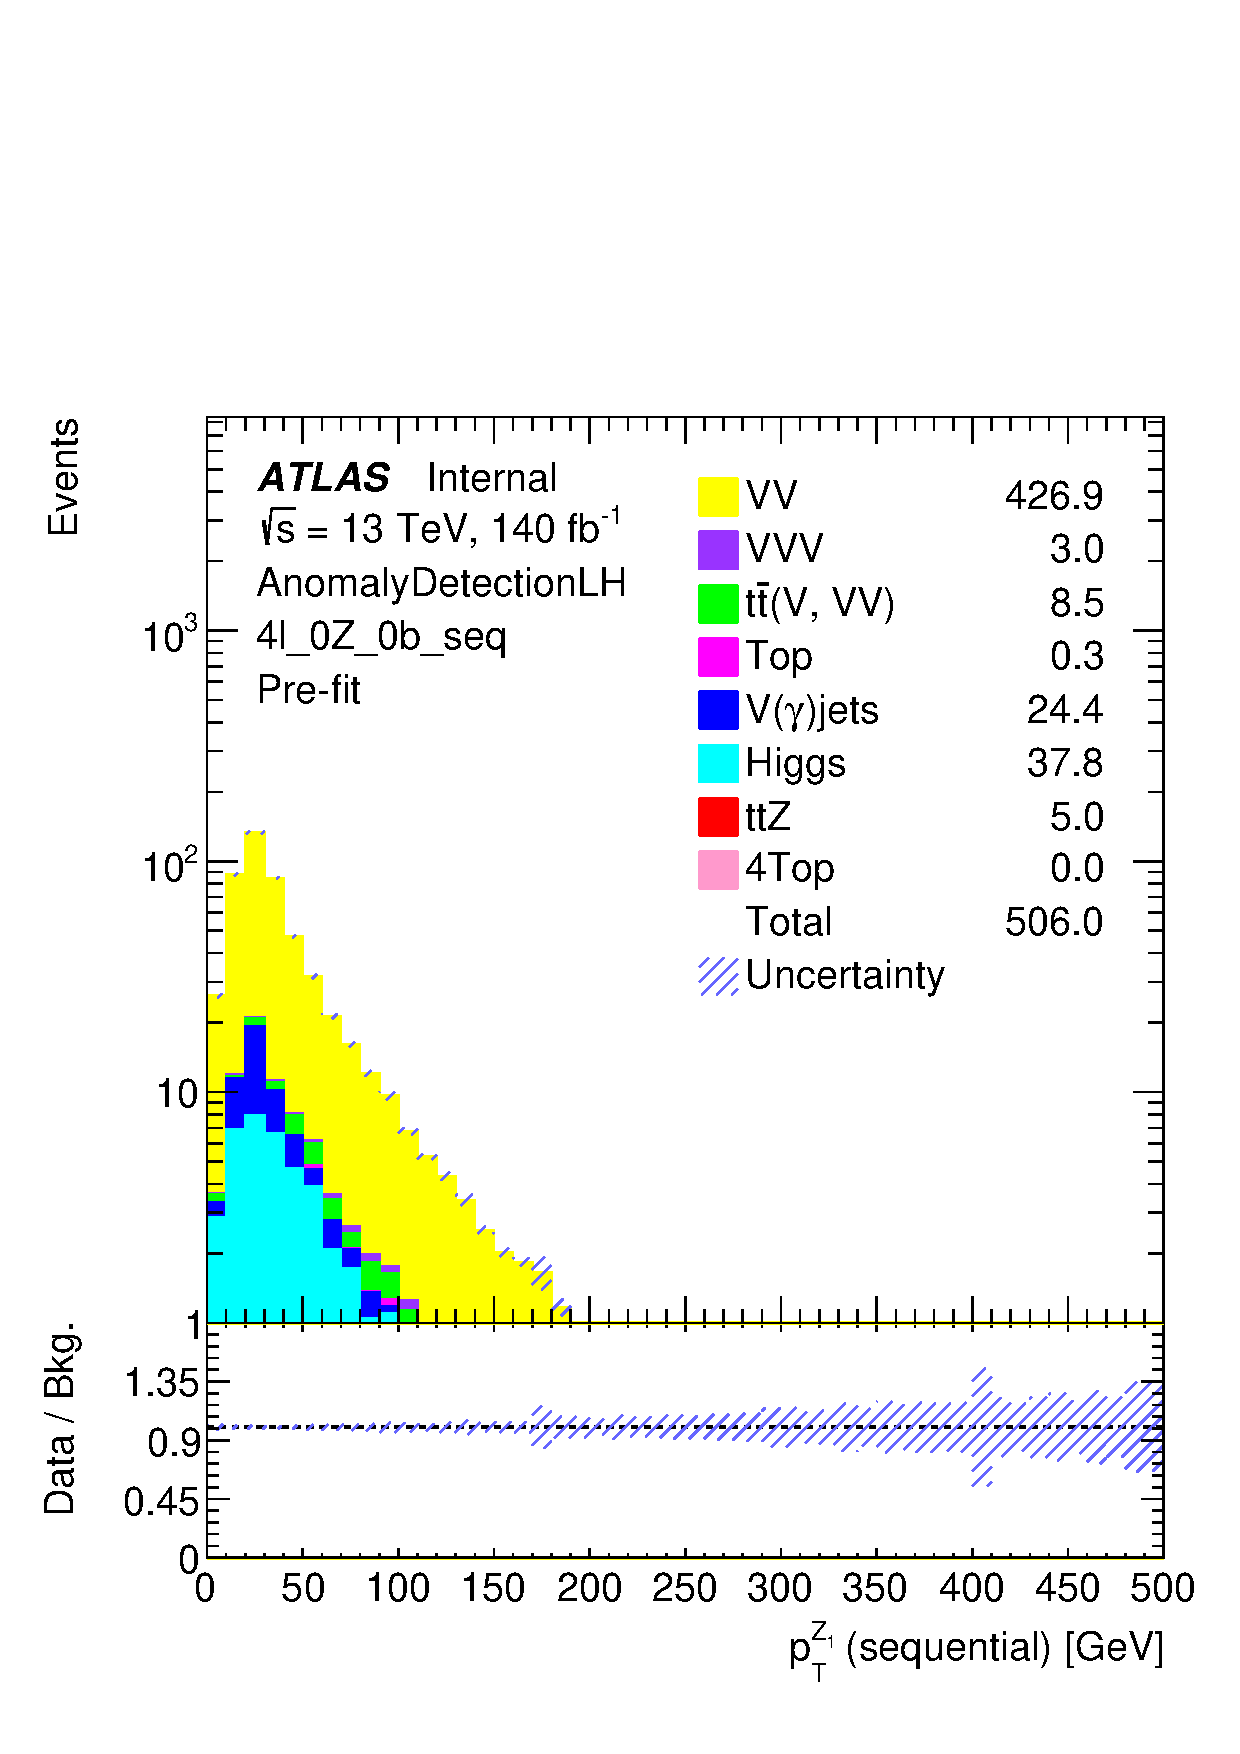
\includegraphics[width=0.24\textwidth]{plots/fourlepLH_run2/Plots/reg_4l_0Z_0b_seq_Z1_pt_seq.pdf} &
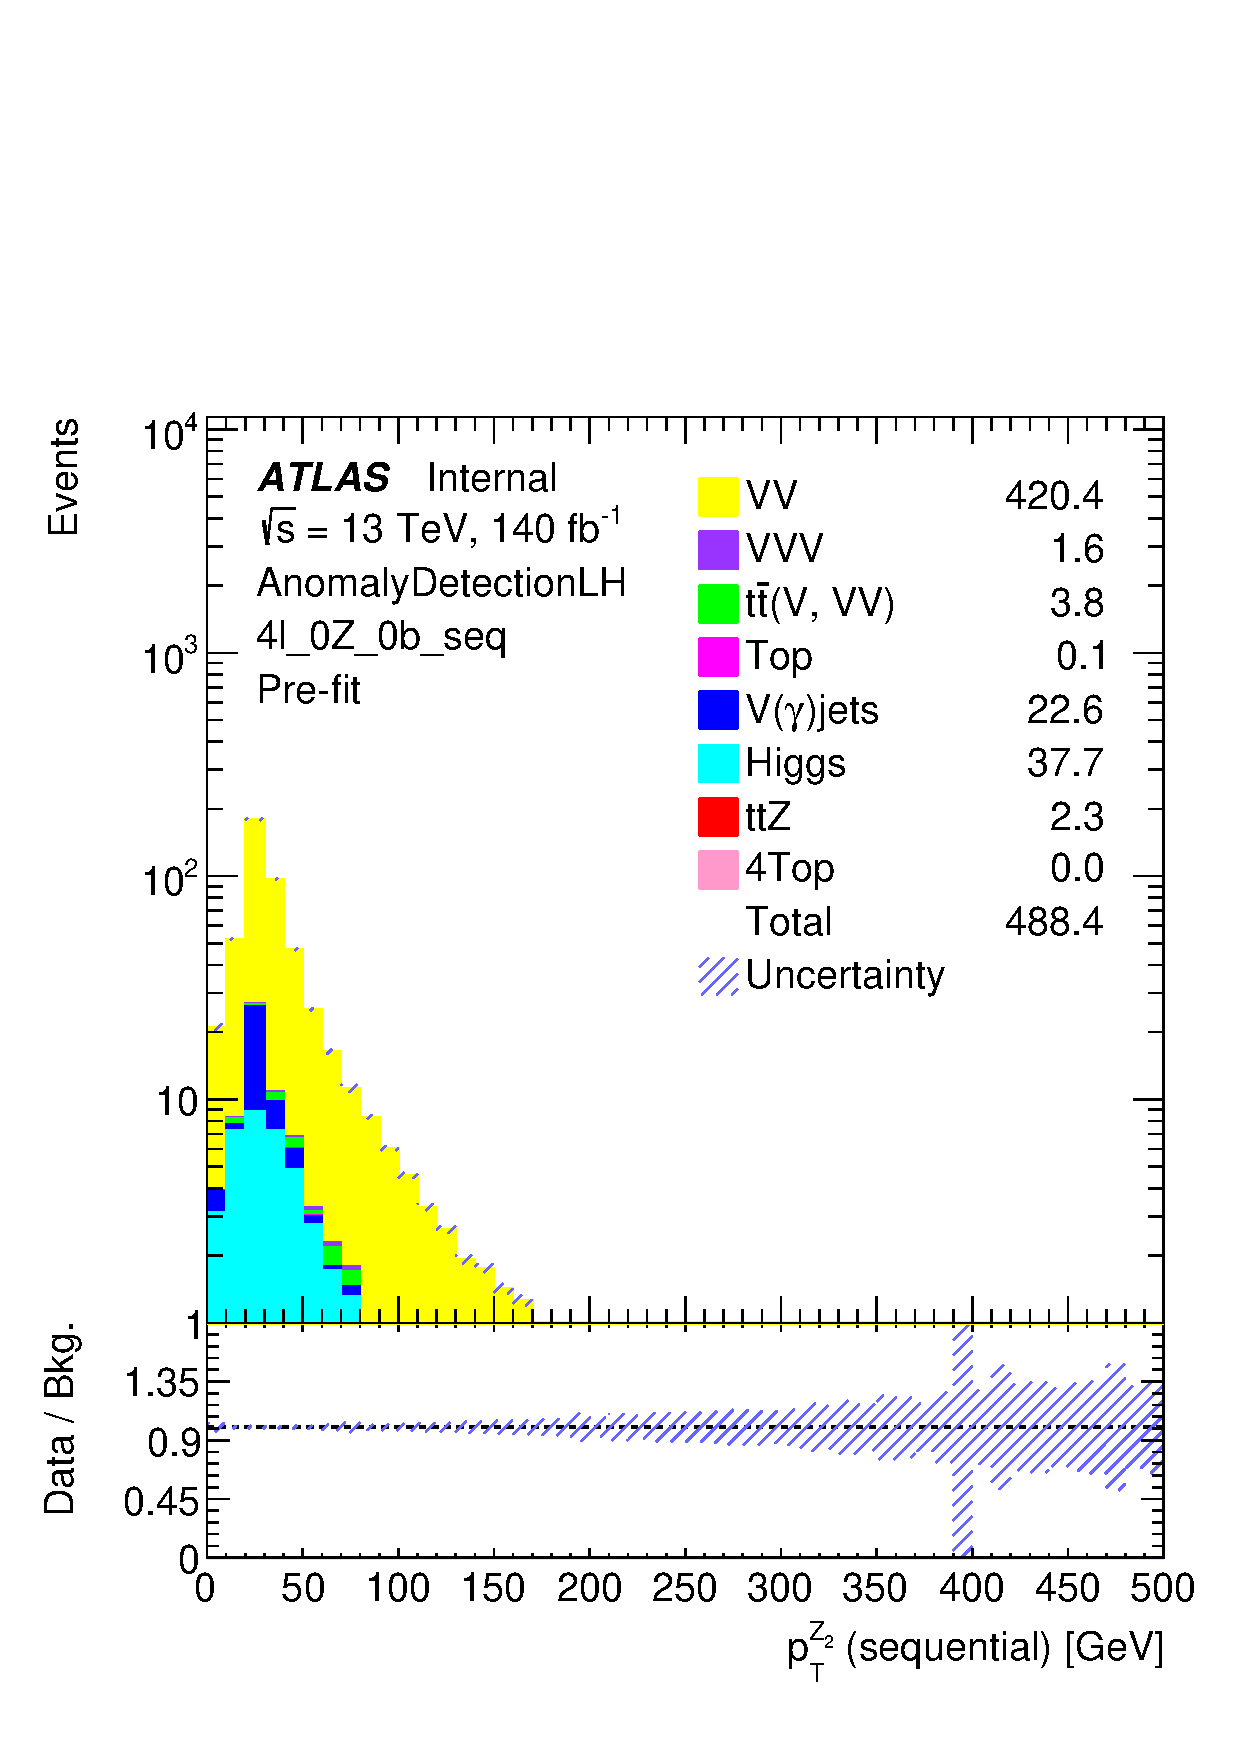
\includegraphics[width=0.24\textwidth]{plots/fourlepLH_run2/Plots/reg_4l_0Z_0b_seq_Z2_pt_seq.pdf}  &

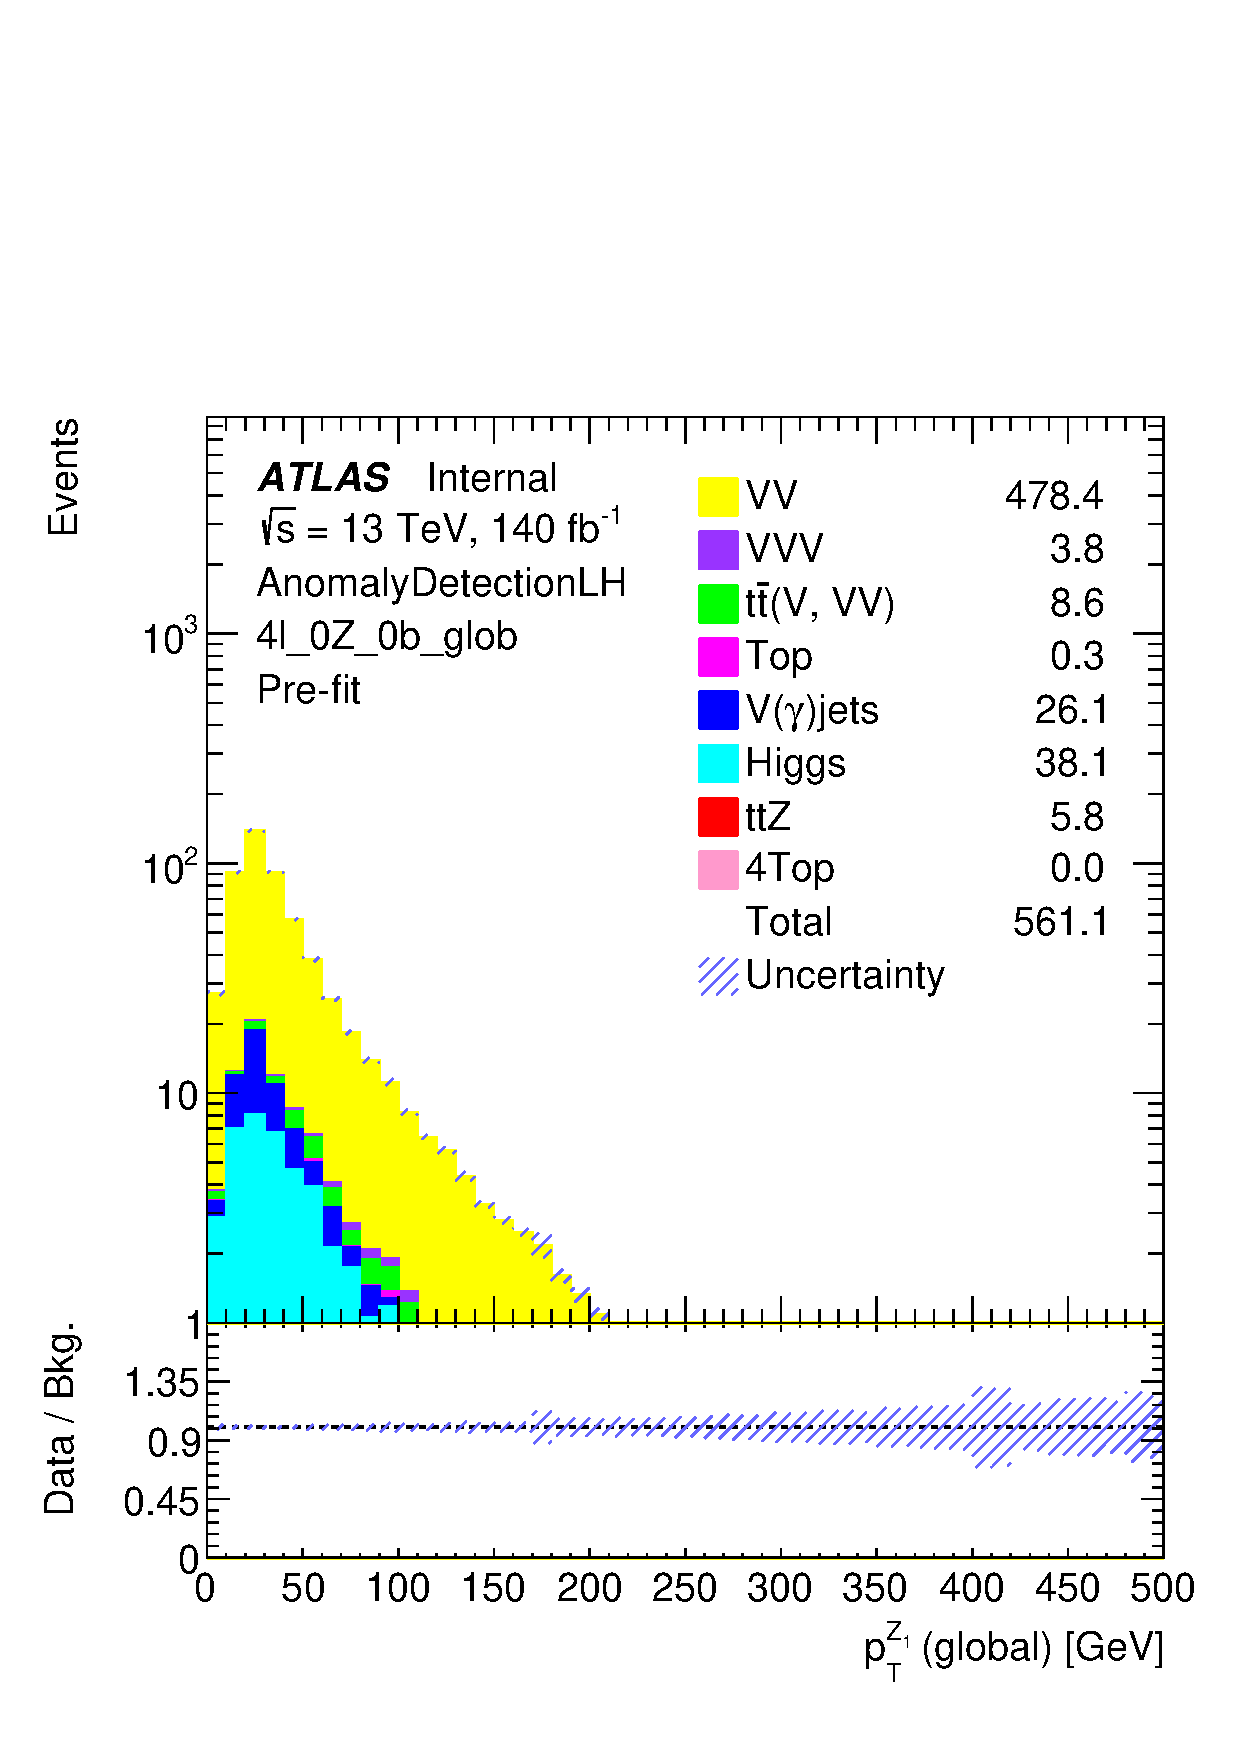
\includegraphics[width=0.24\textwidth]{plots/fourlepLH_run2/Plots/reg_4l_0Z_0b_glob_Z1_pt_glob.pdf} &
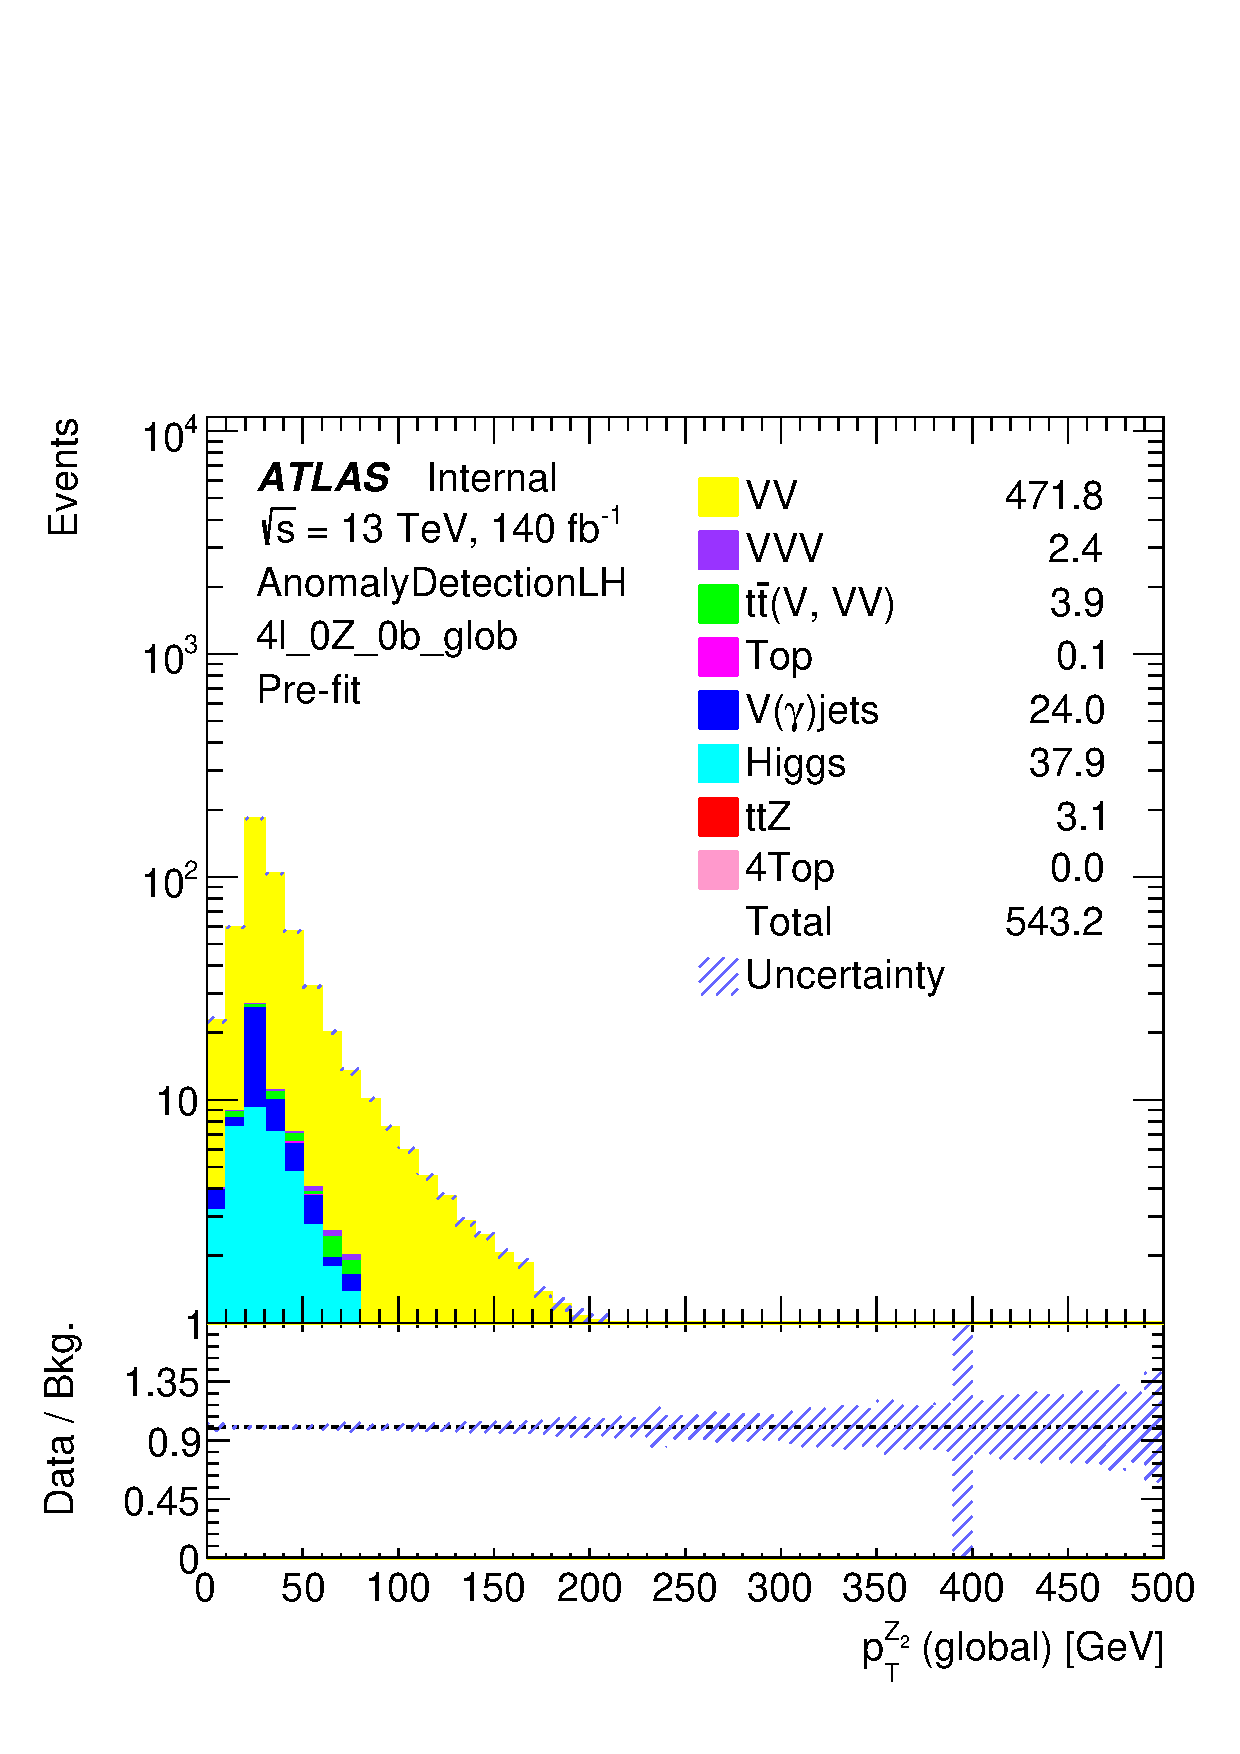
\includegraphics[width=0.24\textwidth]{plots/fourlepLH_run2/Plots/reg_4l_0Z_0b_glob_Z2_pt_glob.pdf}
\end{tabular}
\end{frame}

\begin{frame}{\texttt{Results: 4l\_0Z\_0b}}
\begin{tabular}{cccccc}
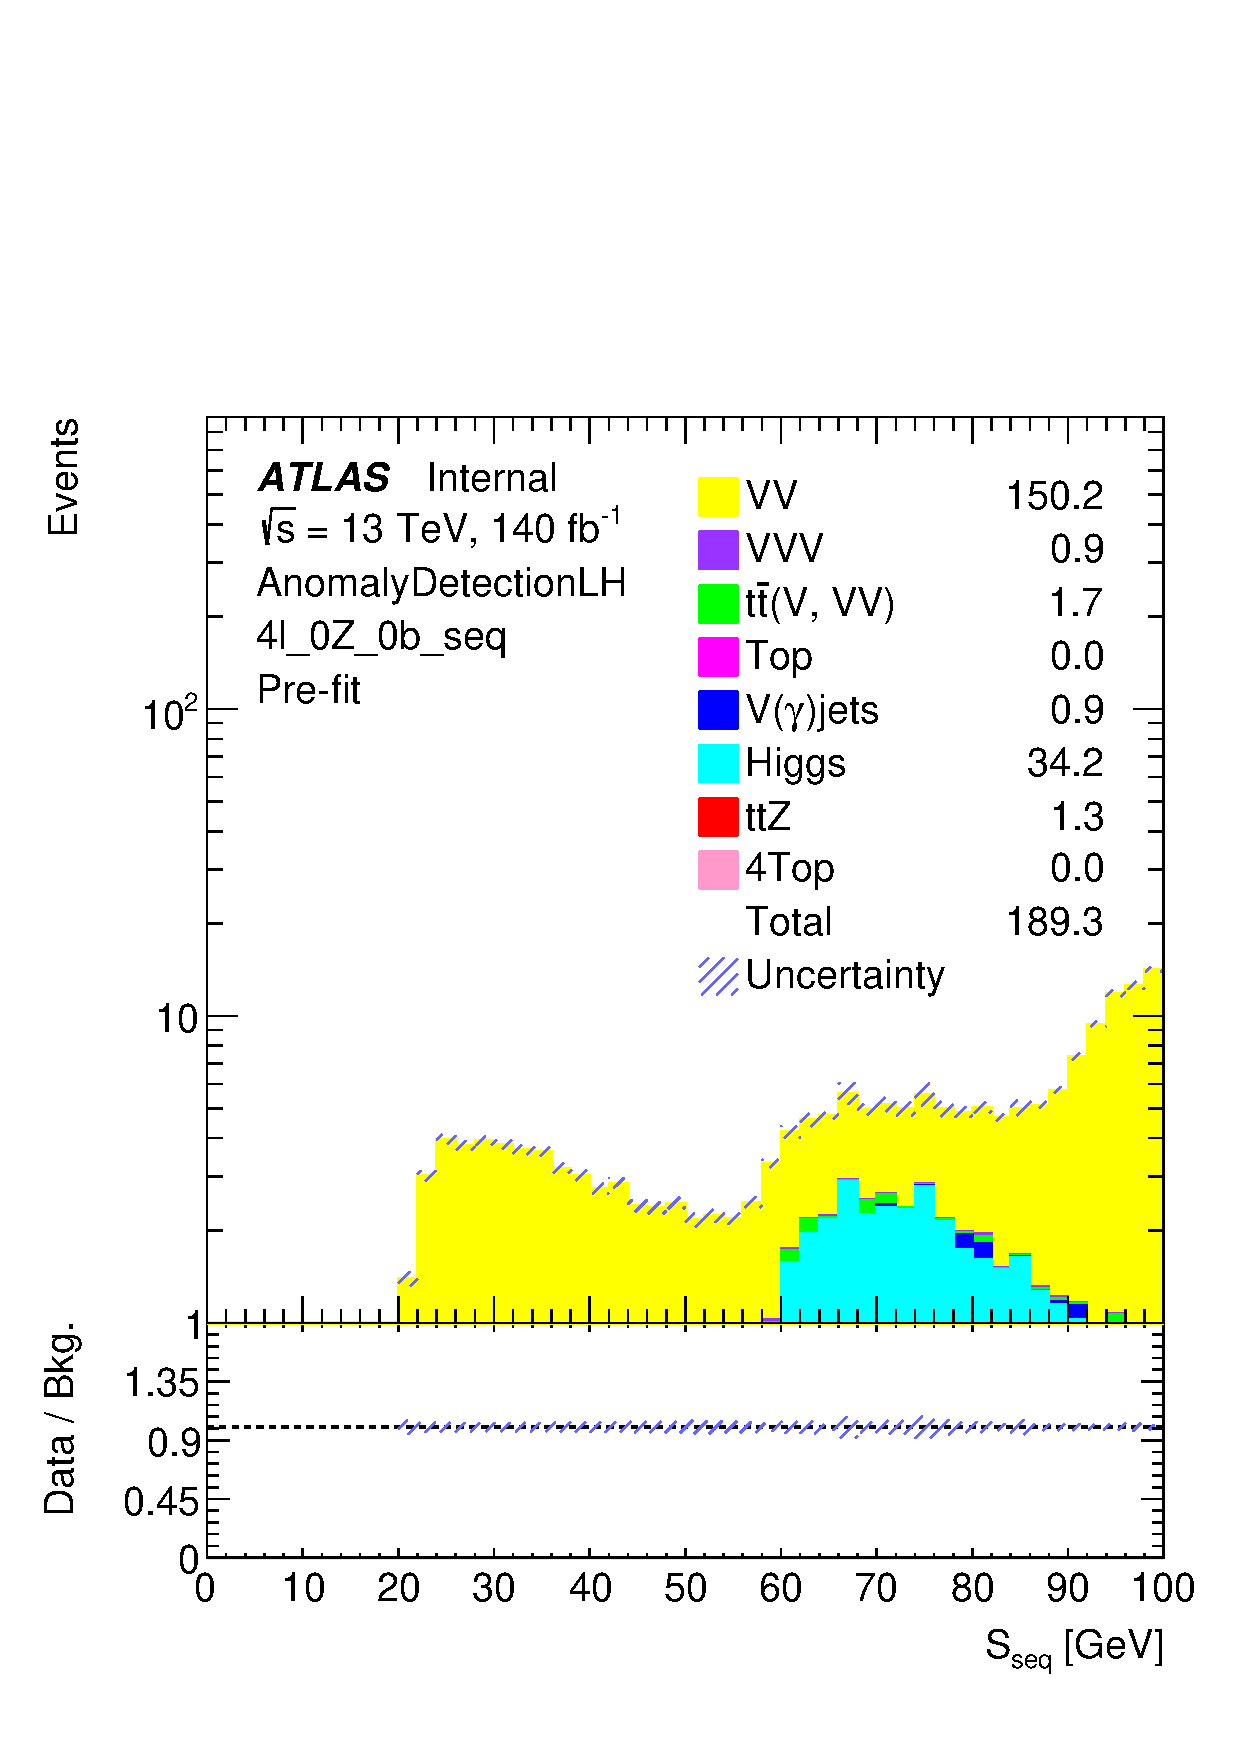
\includegraphics[width=0.24\textwidth]{plots/fourlepLH_run2/Plots/reg_4l_0Z_0b_seq_Zscore_seq.pdf} & 
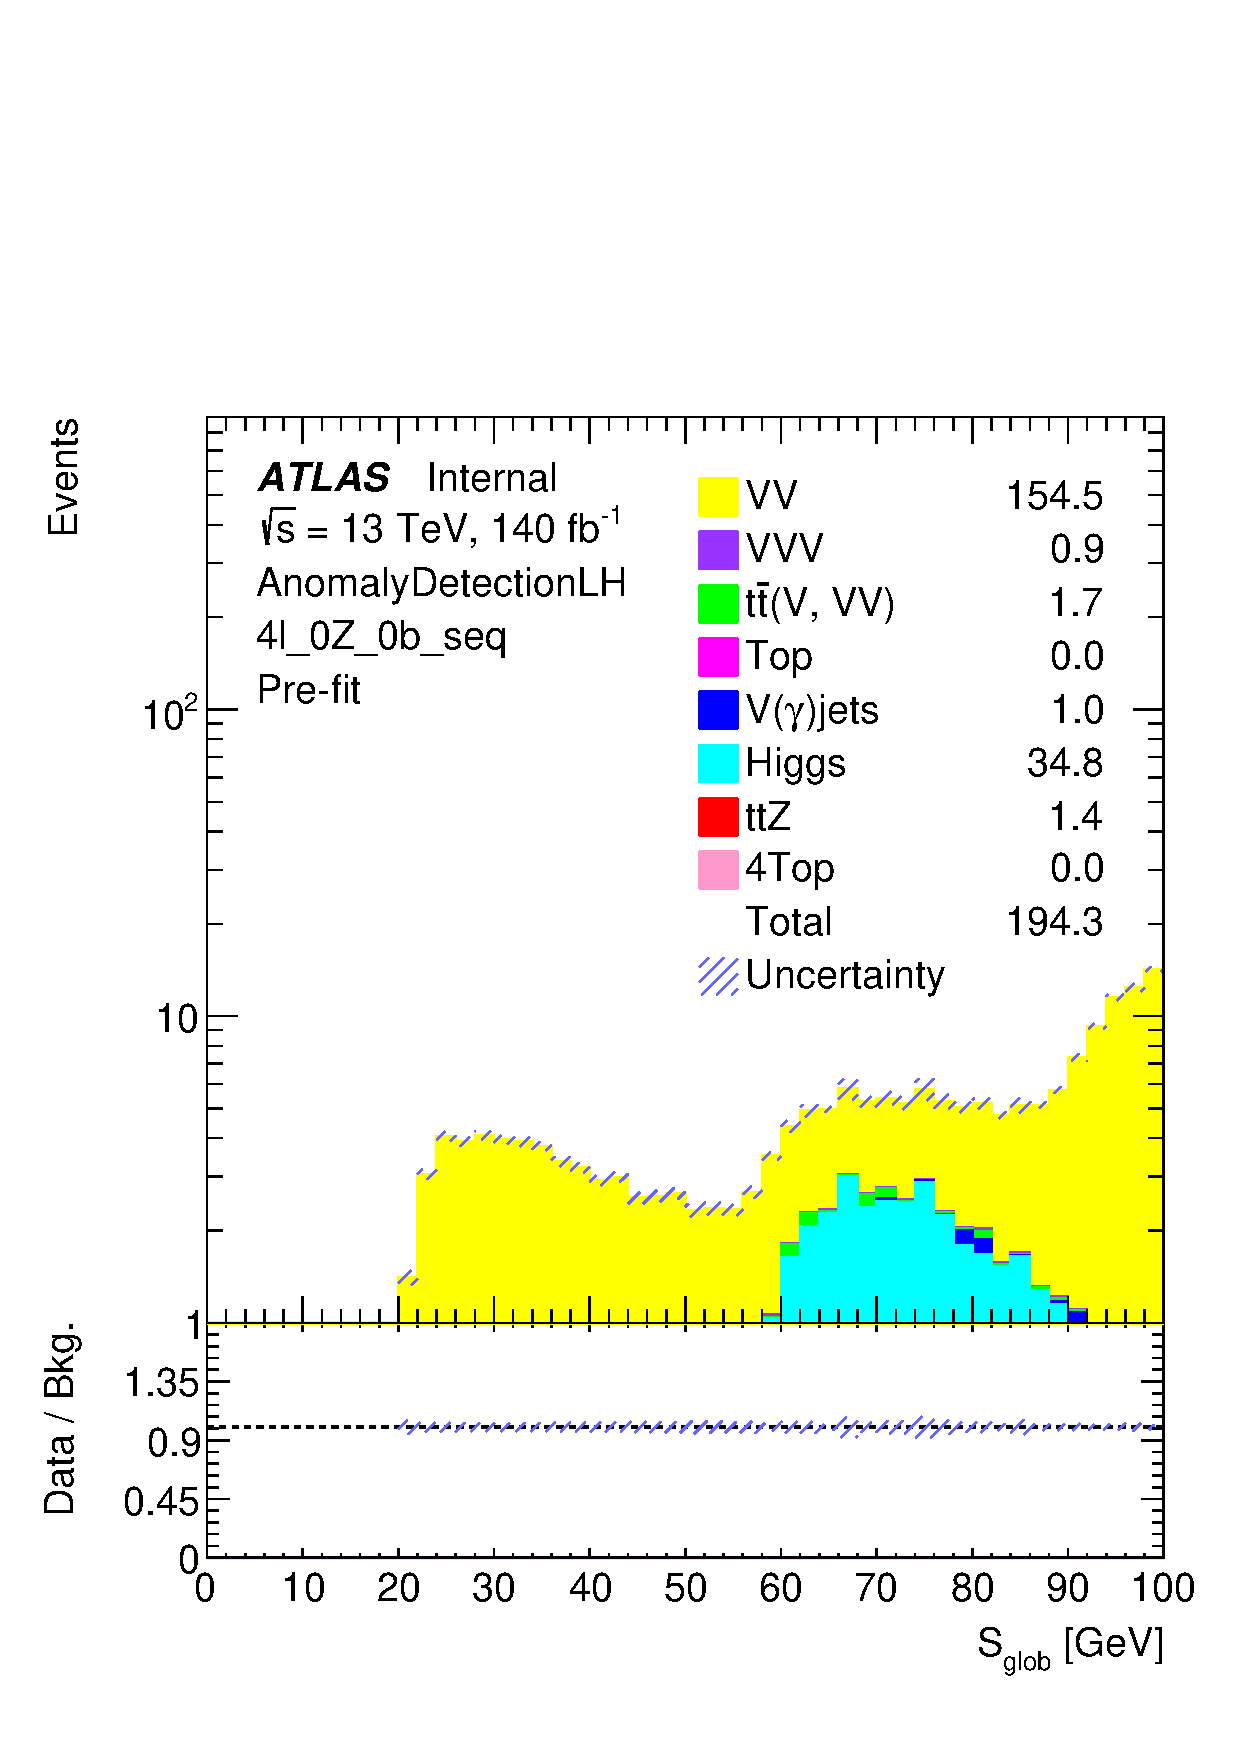
\includegraphics[width=0.24\textwidth]{plots/fourlepLH_run2/Plots/reg_4l_0Z_0b_seq_Zscore_glob.pdf}&
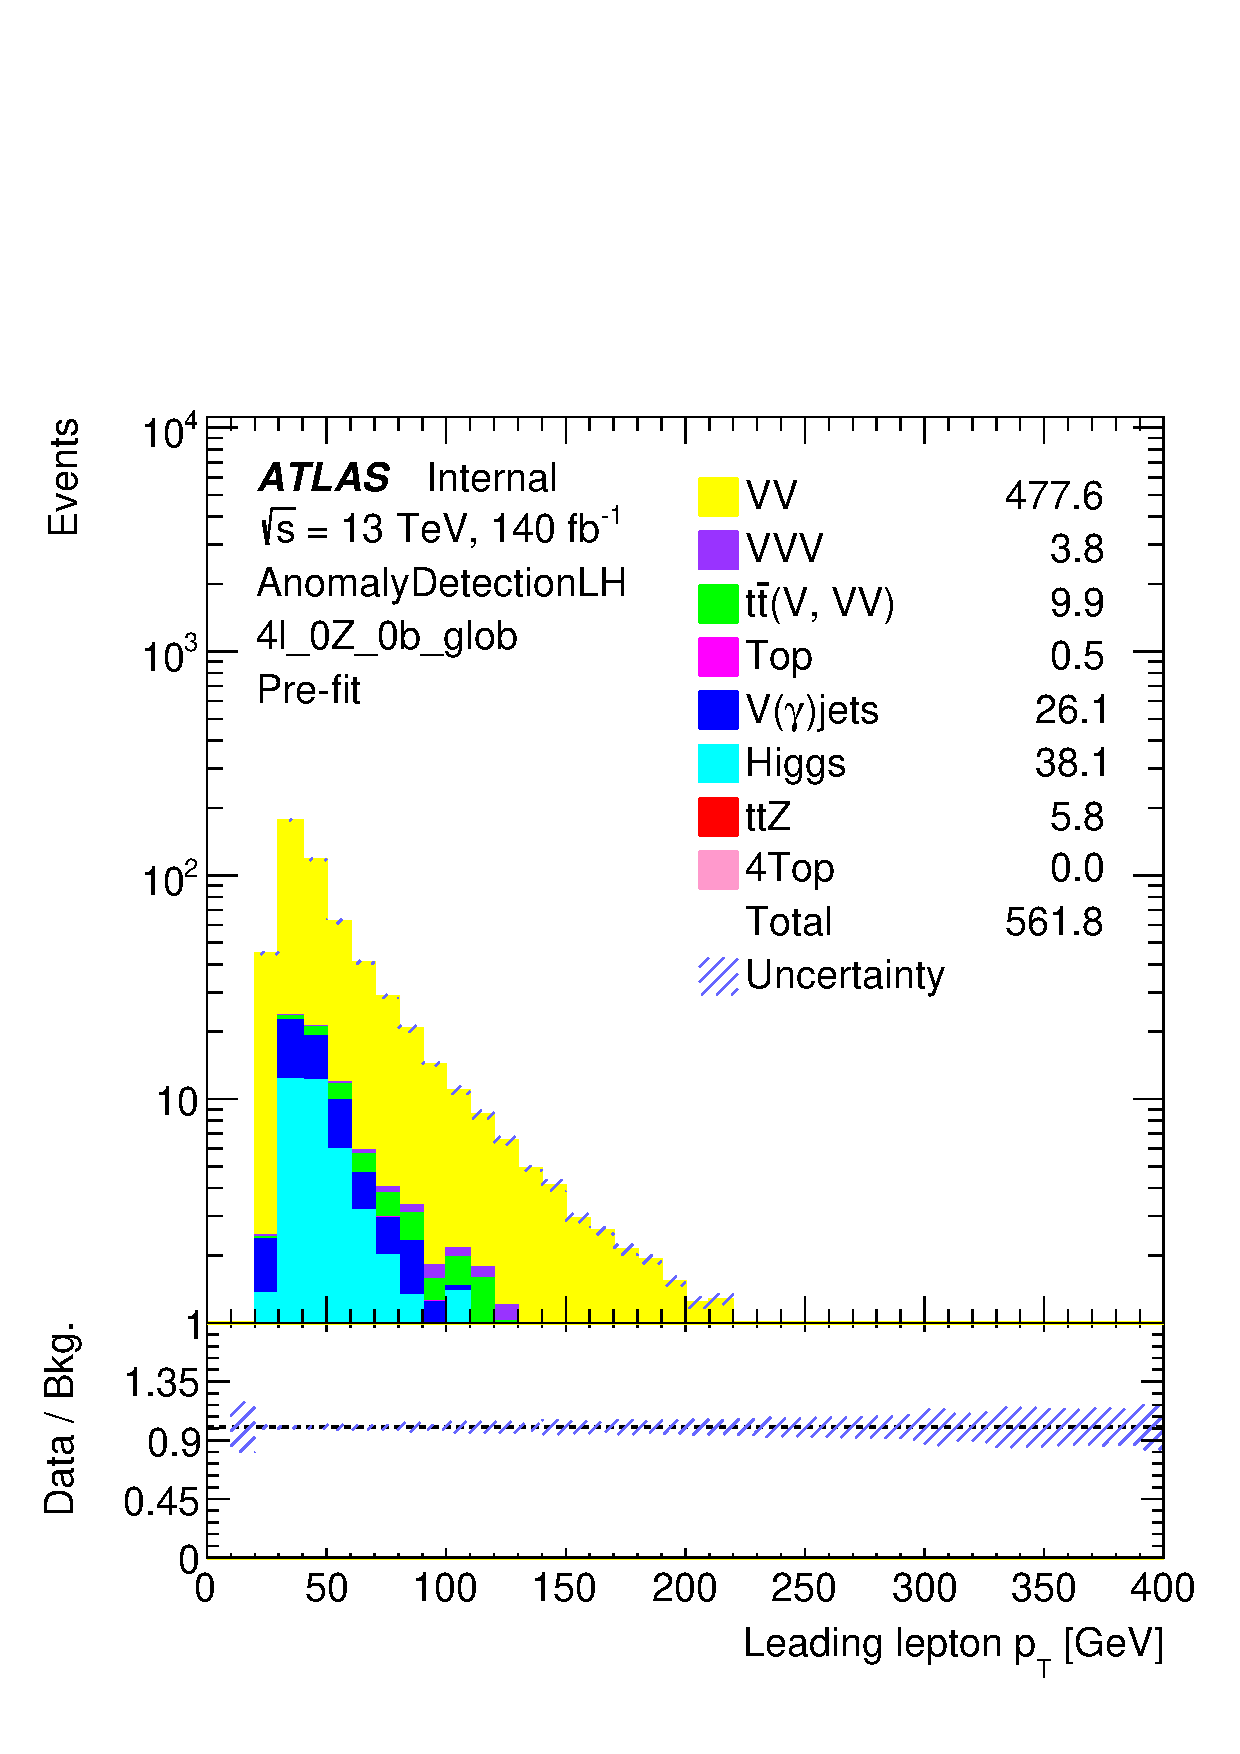
\includegraphics[width=0.24\textwidth]{plots/fourlepLH_run2/Plots/reg_4l_0Z_0b_seq_deltaZscore.pdf}\\

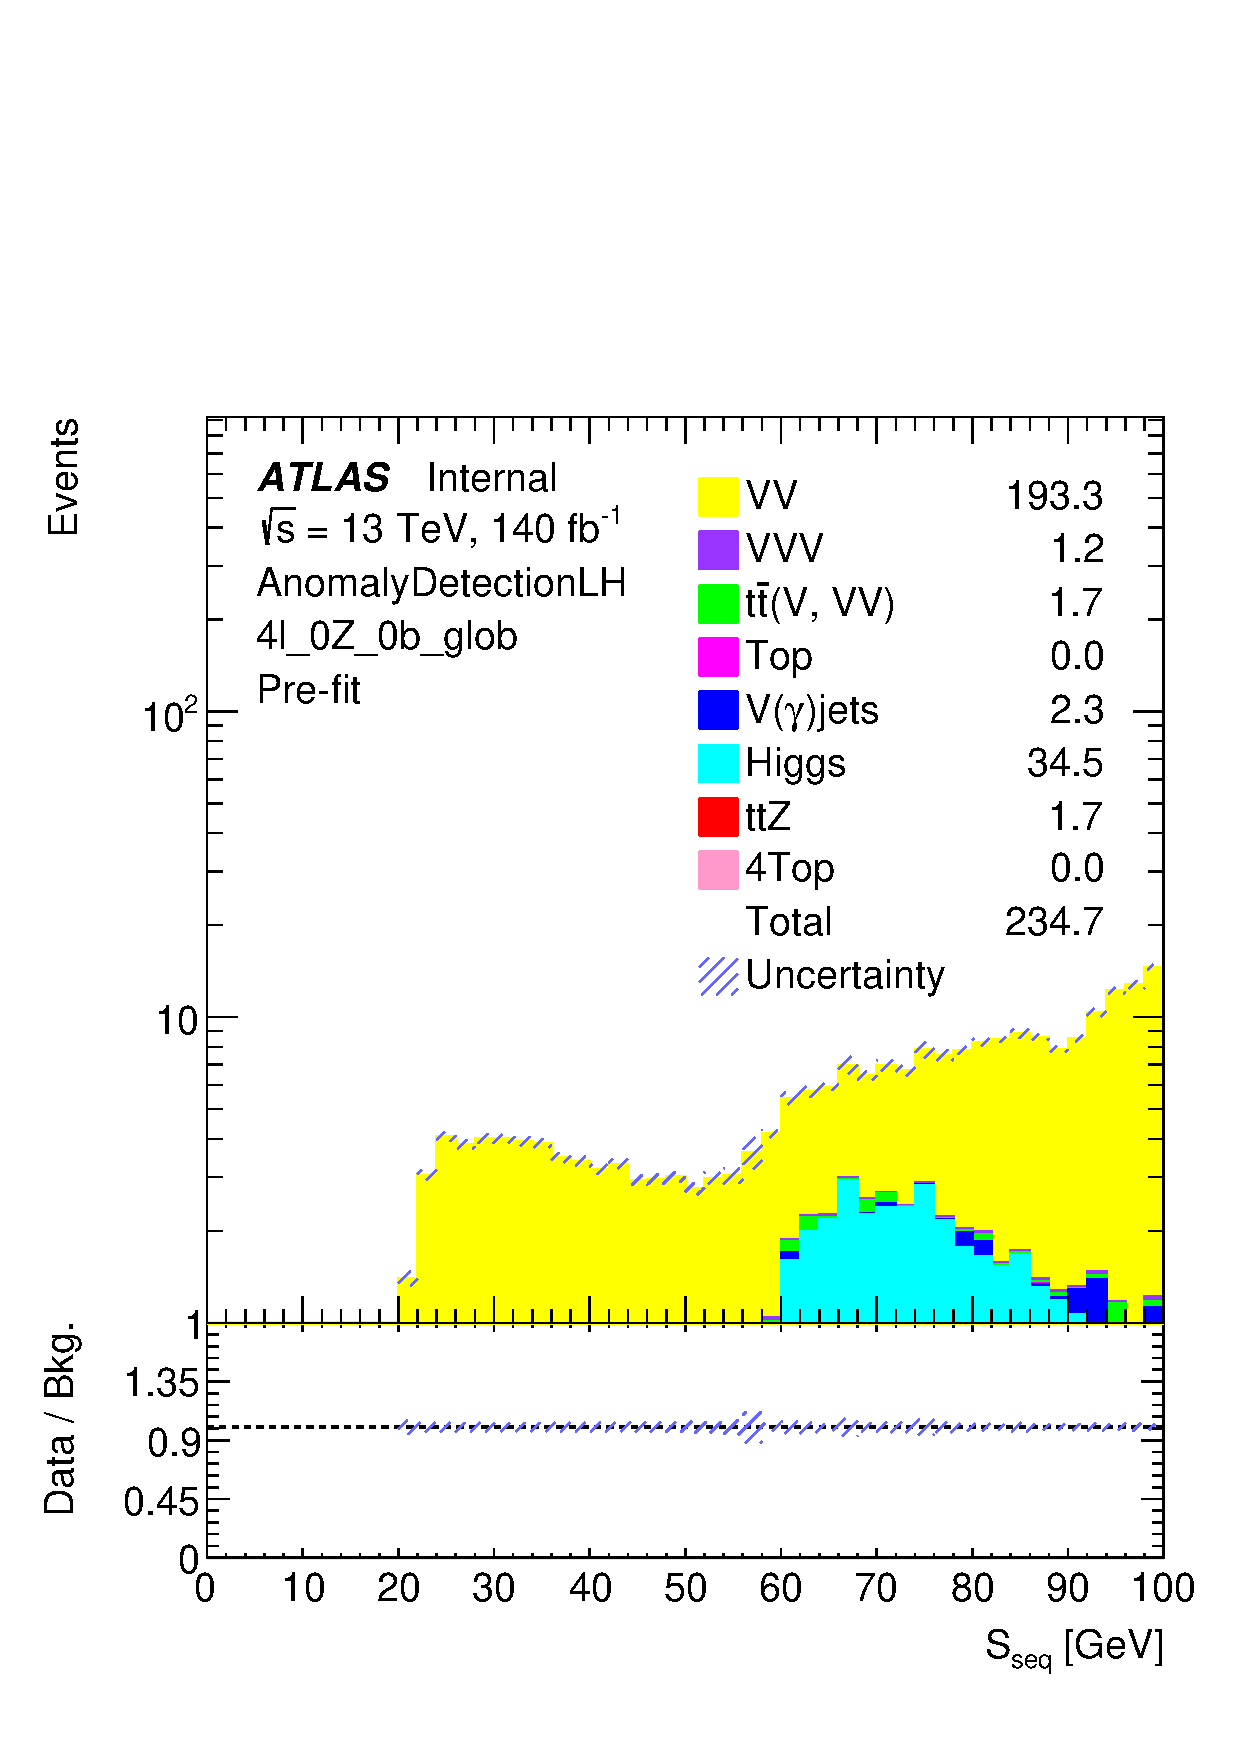
\includegraphics[width=0.24\textwidth]{plots/fourlepLH_run2/Plots/reg_4l_0Z_0b_glob_Zscore_seq.pdf} & 
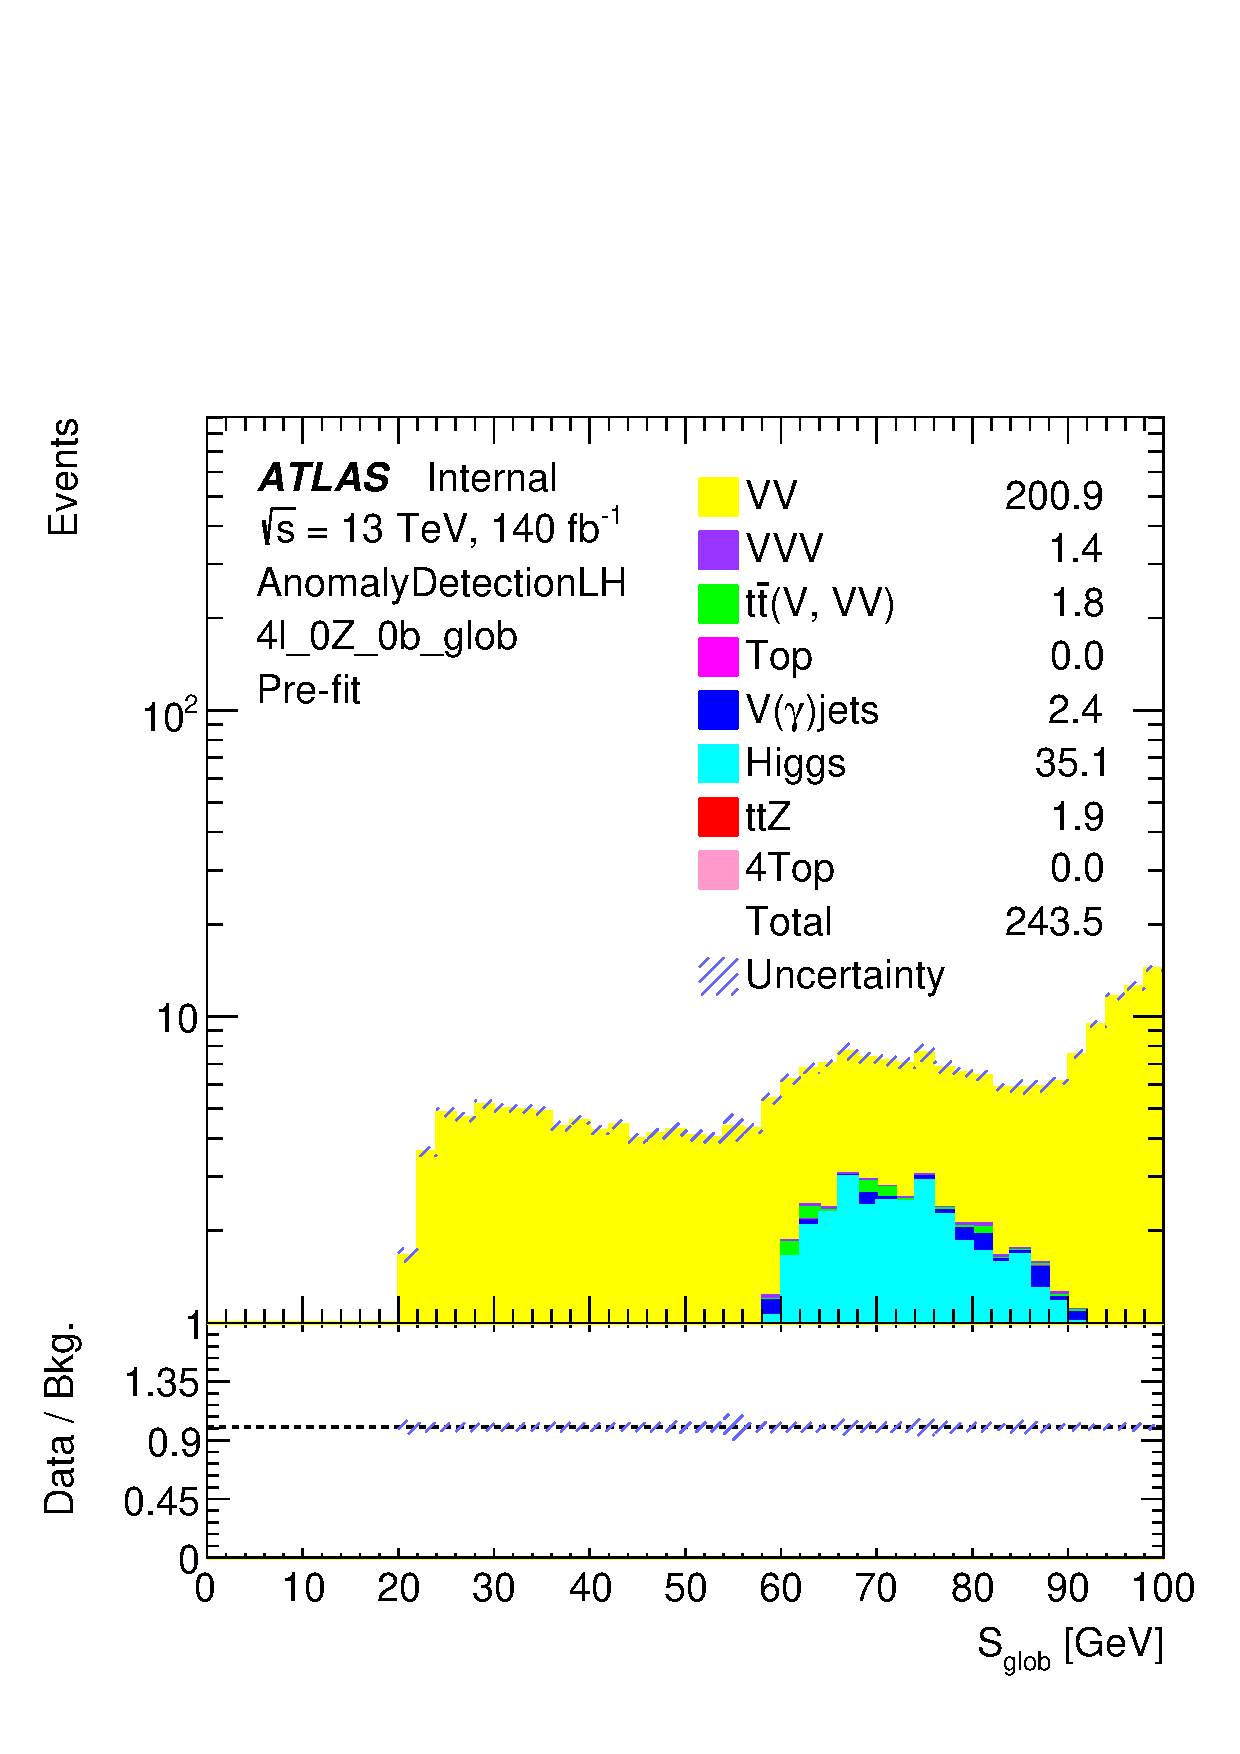
\includegraphics[width=0.24\textwidth]{plots/fourlepLH_run2/Plots/reg_4l_0Z_0b_glob_Zscore_glob.pdf}&
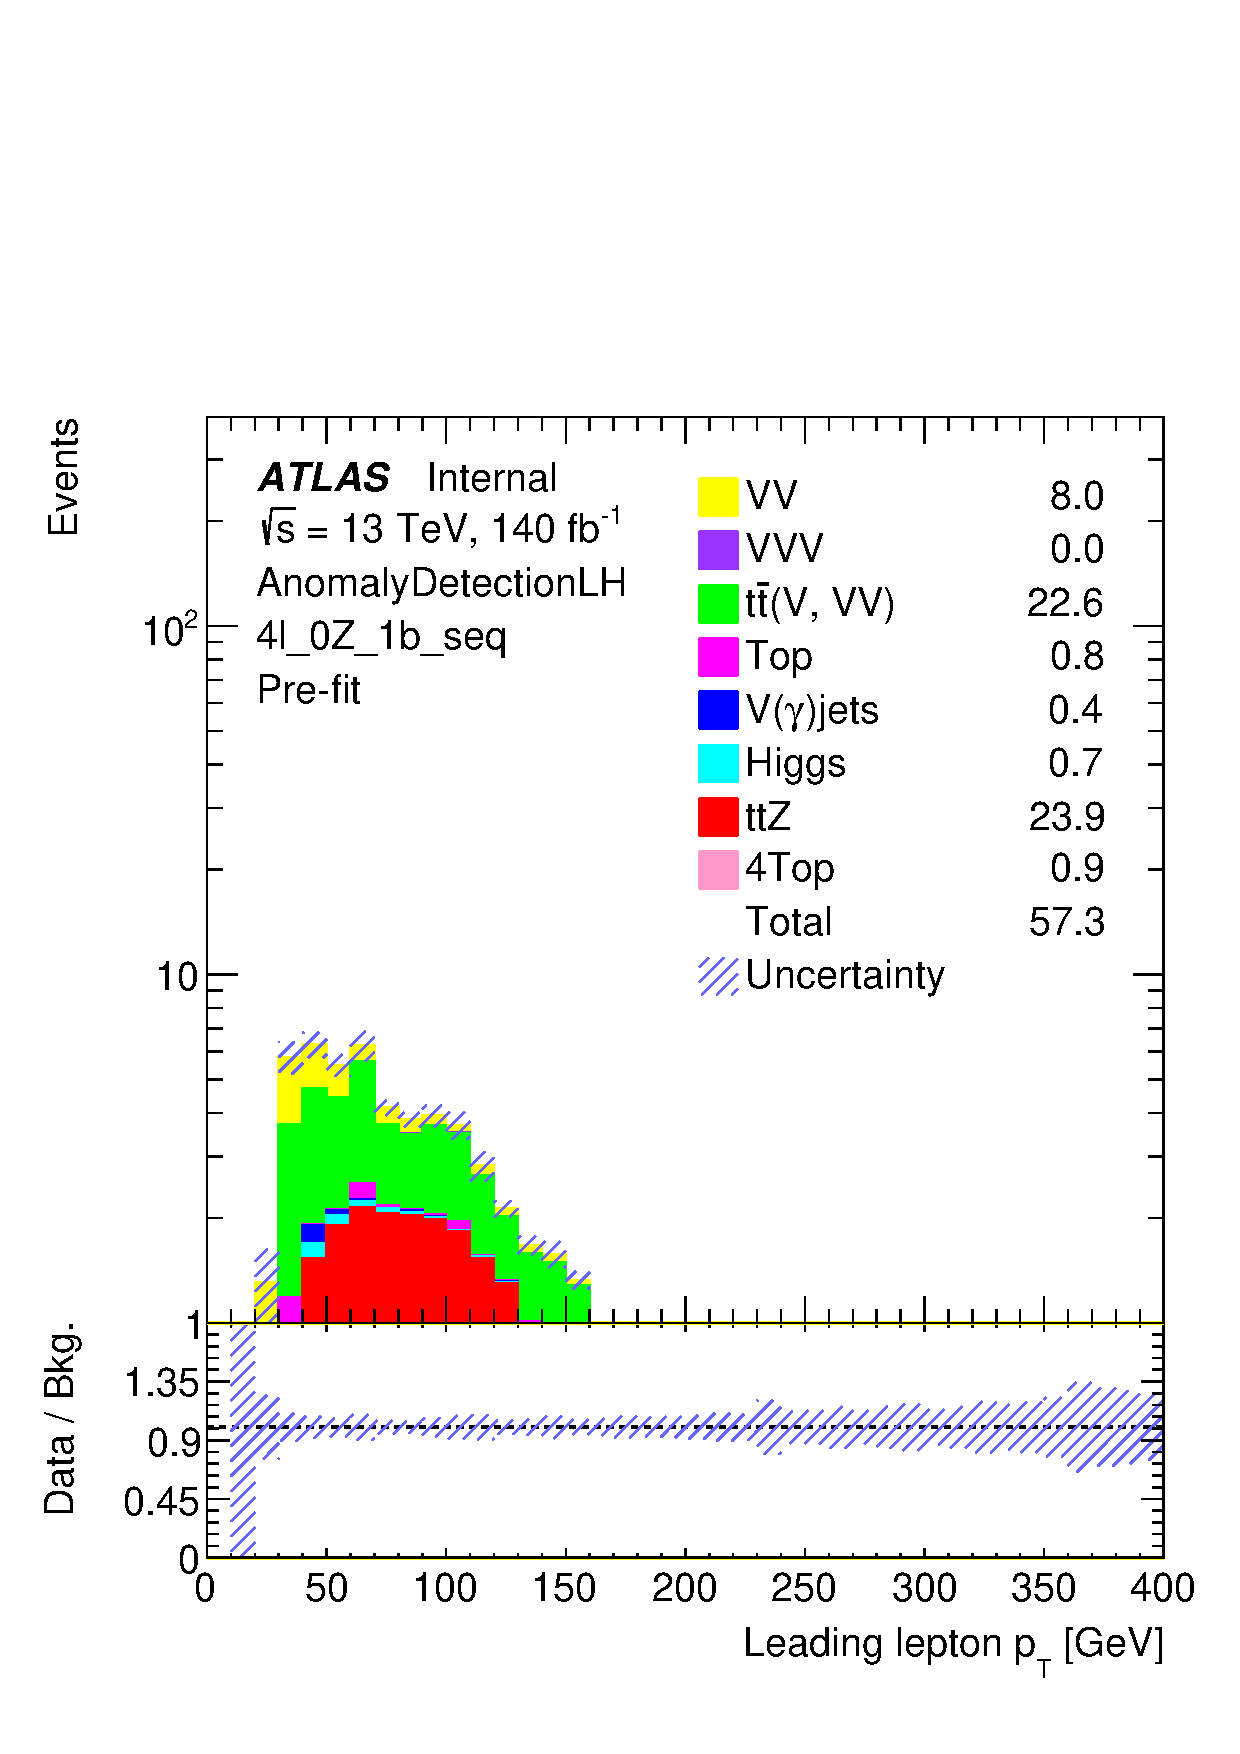
\includegraphics[width=0.24\textwidth]{plots/fourlepLH_run2/Plots/reg_4l_0Z_0b_glob_deltaZscore.pdf}
\end{tabular}
\end{frame}


\begin{frame}{\texttt{Results: 4l\_0Z\_0b}}
\begin{tabular}{cccccc}

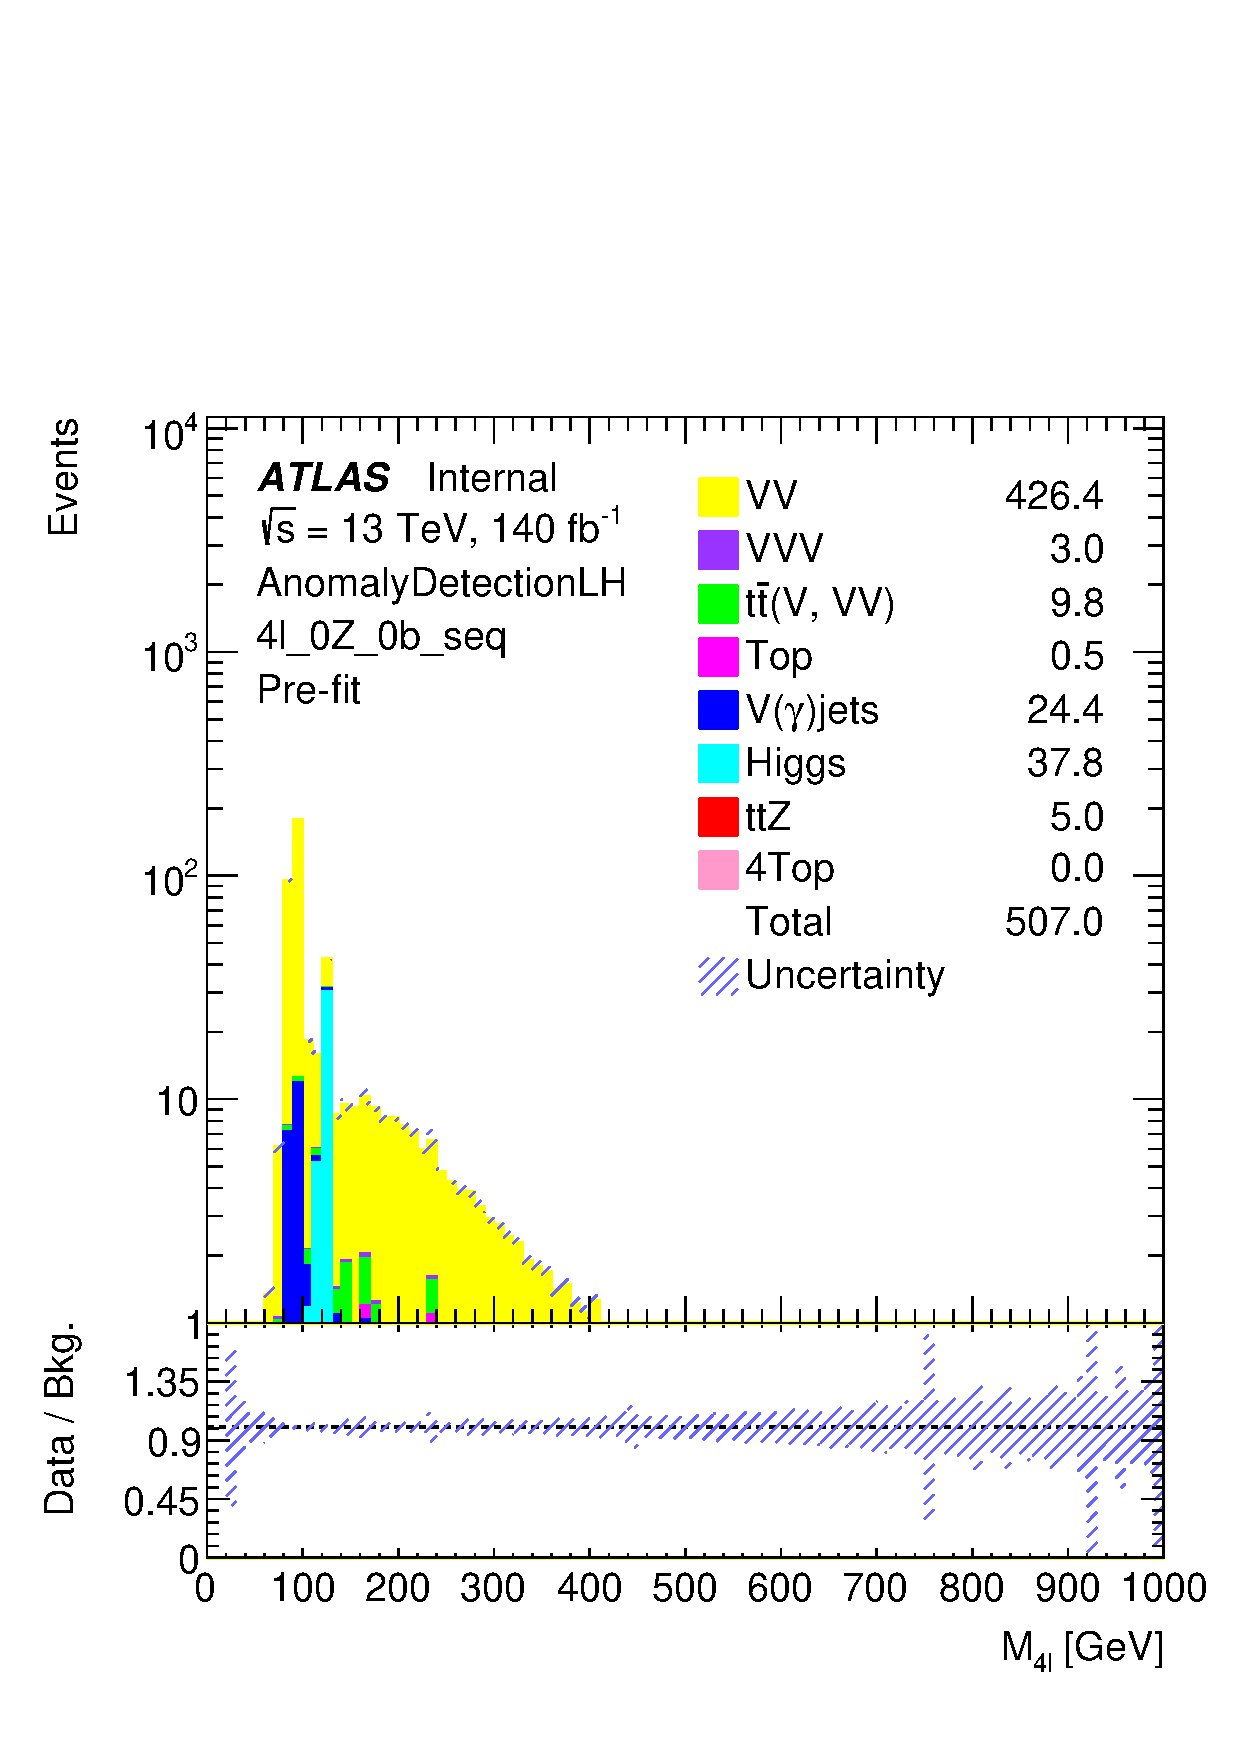
\includegraphics[width=0.24\textwidth]{plots/fourlepLH_run2/Plots/reg_4l_0Z_0b_seq_m4l.pdf} &
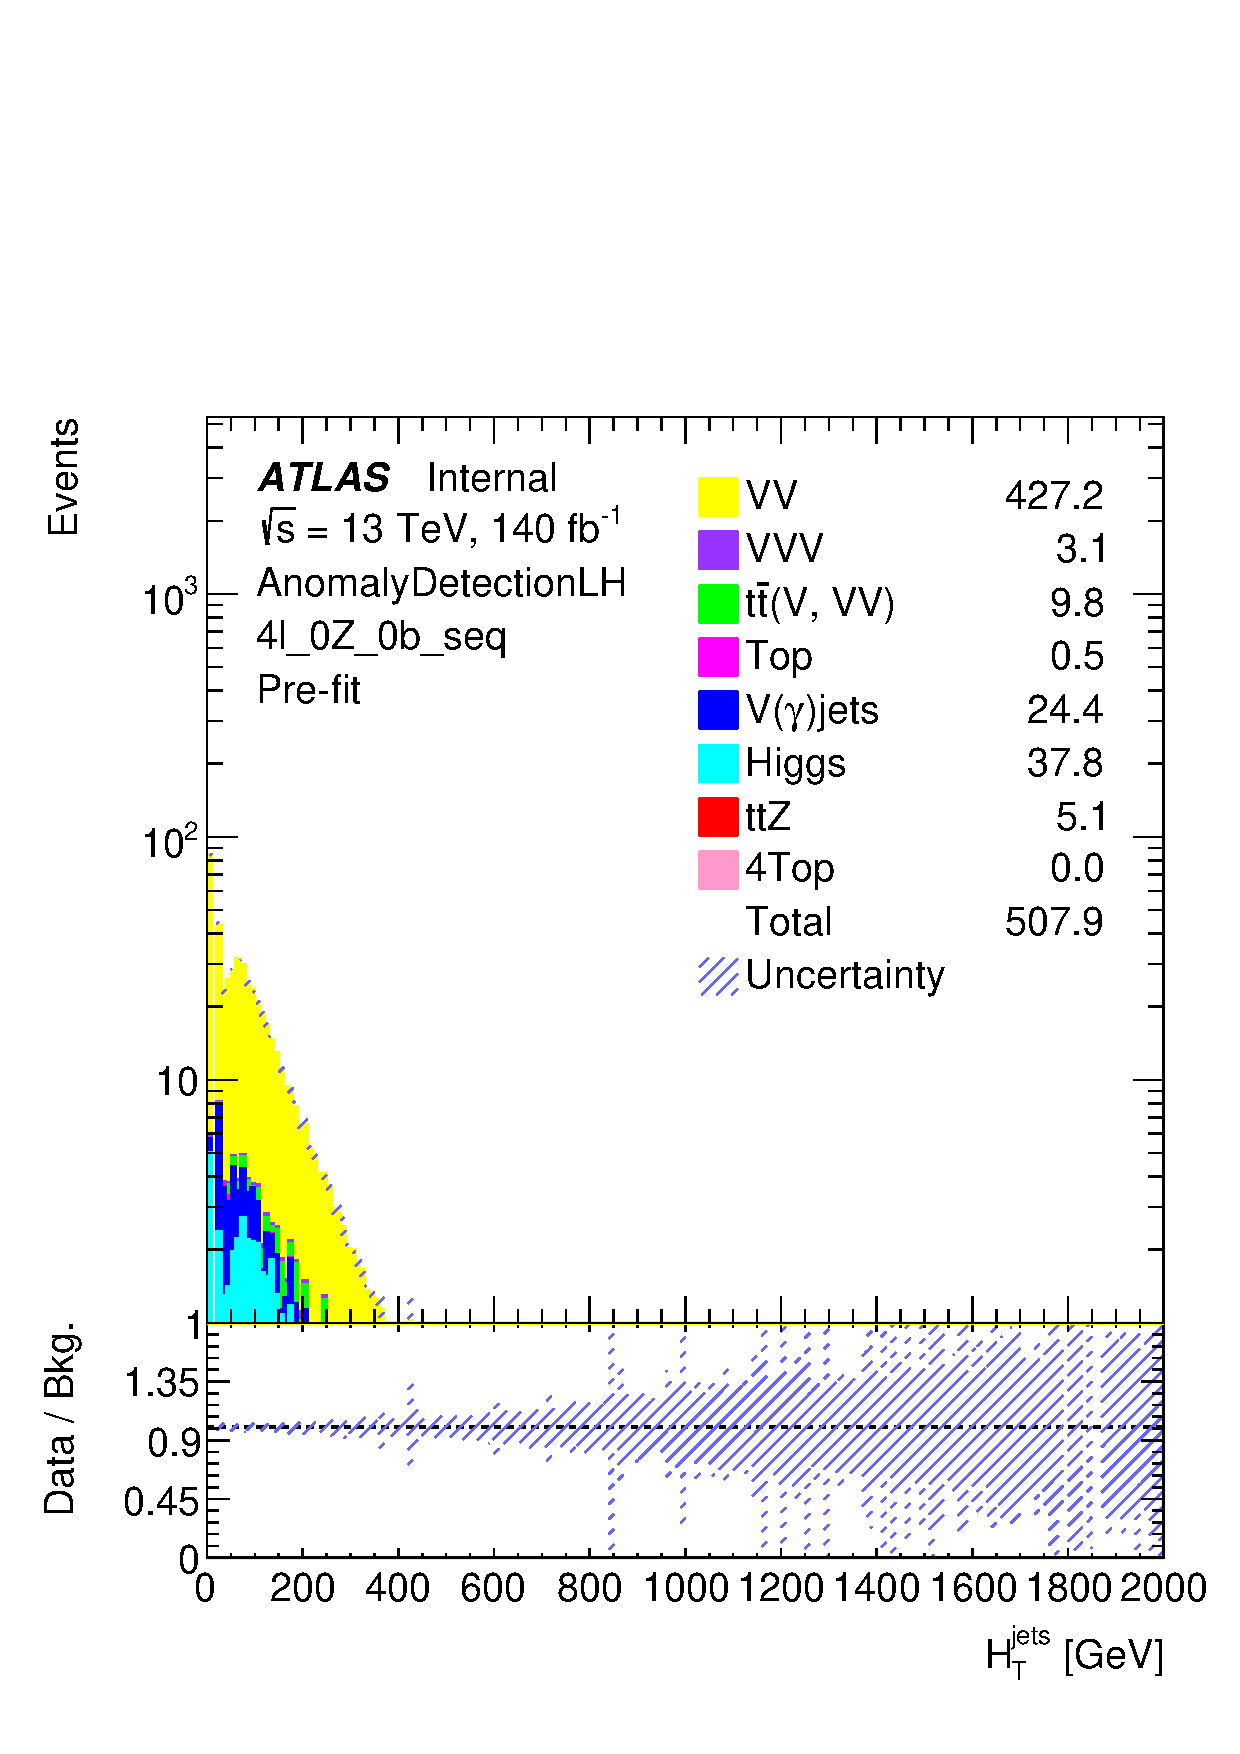
\includegraphics[width=0.24\textwidth]{plots/fourlepLH_run2/Plots/reg_4l_0Z_0b_seq_HT_jets.pdf} &
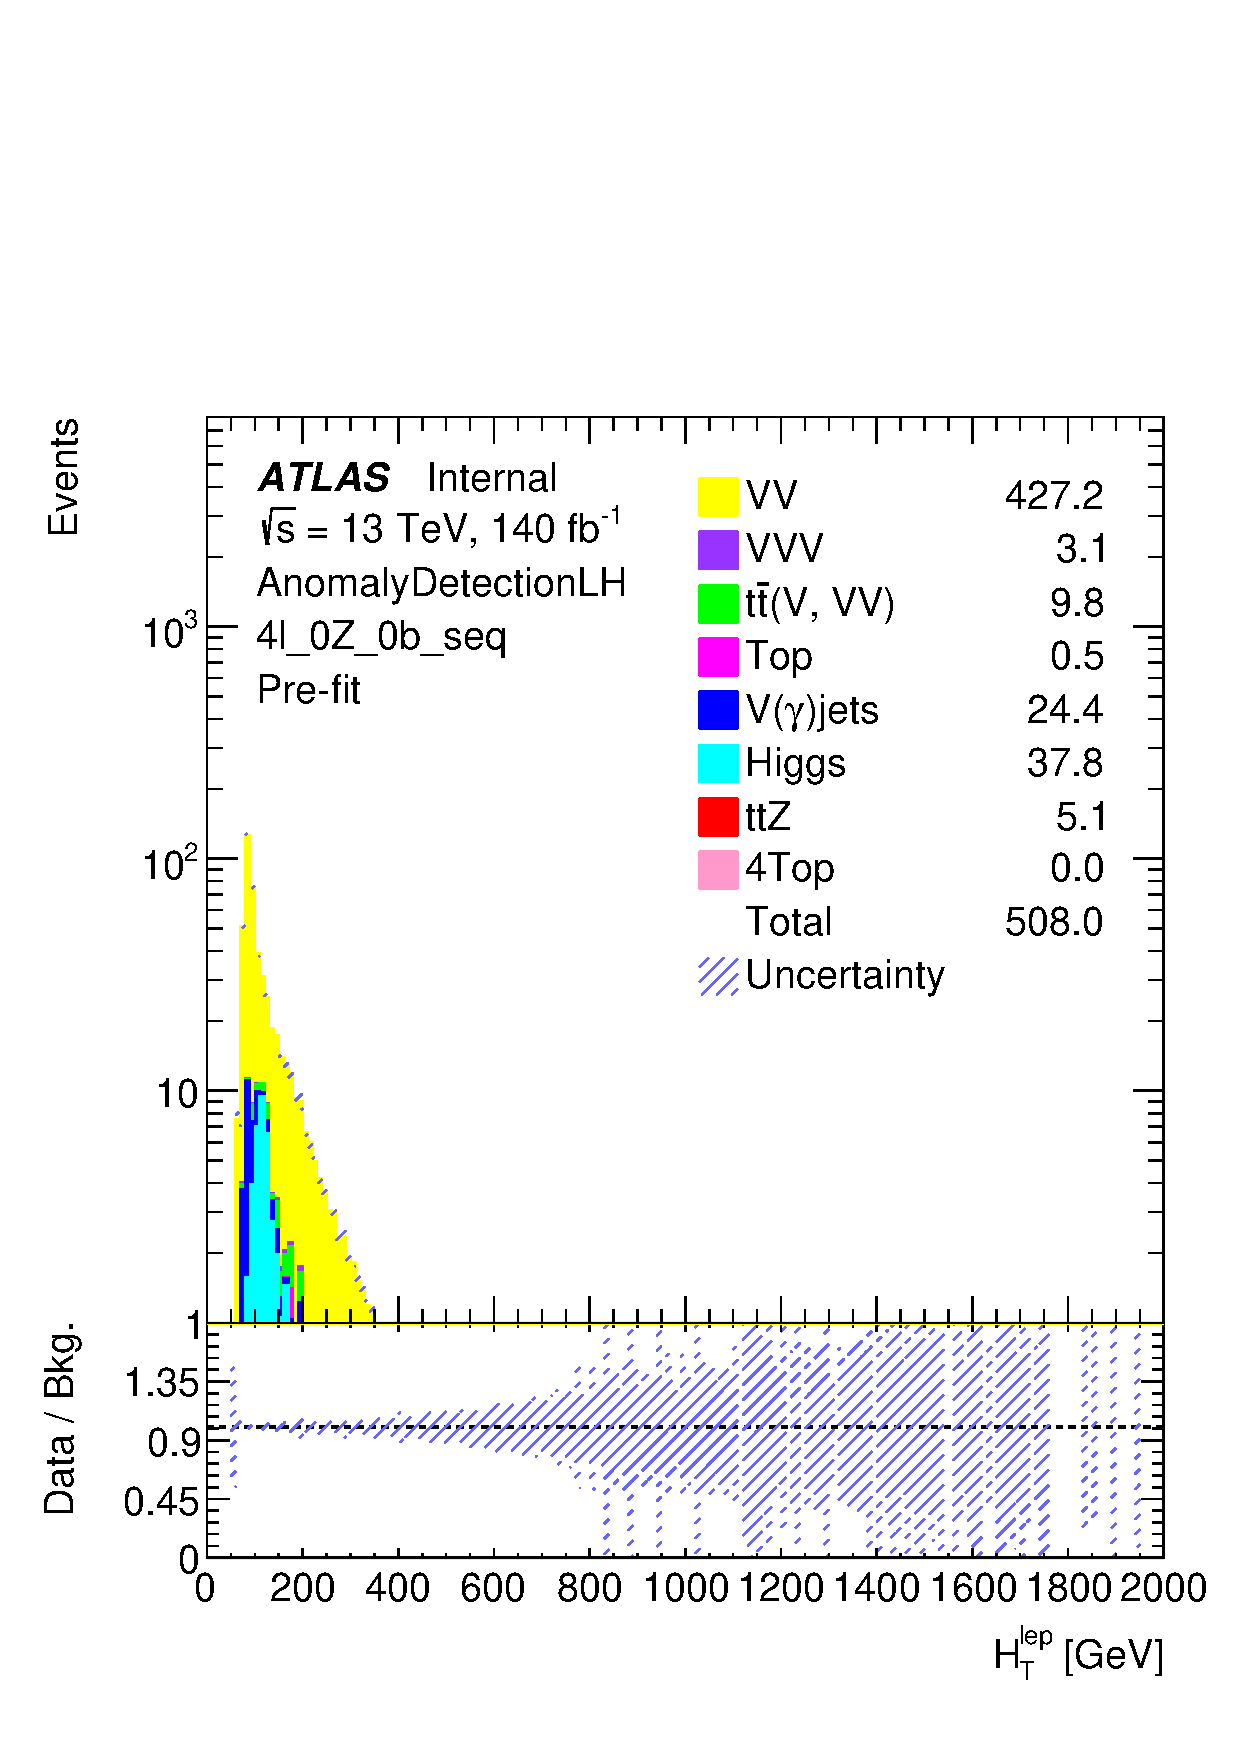
\includegraphics[width=0.24\textwidth]{plots/fourlepLH_run2/Plots/reg_4l_0Z_0b_seq_HT_lep.pdf} &
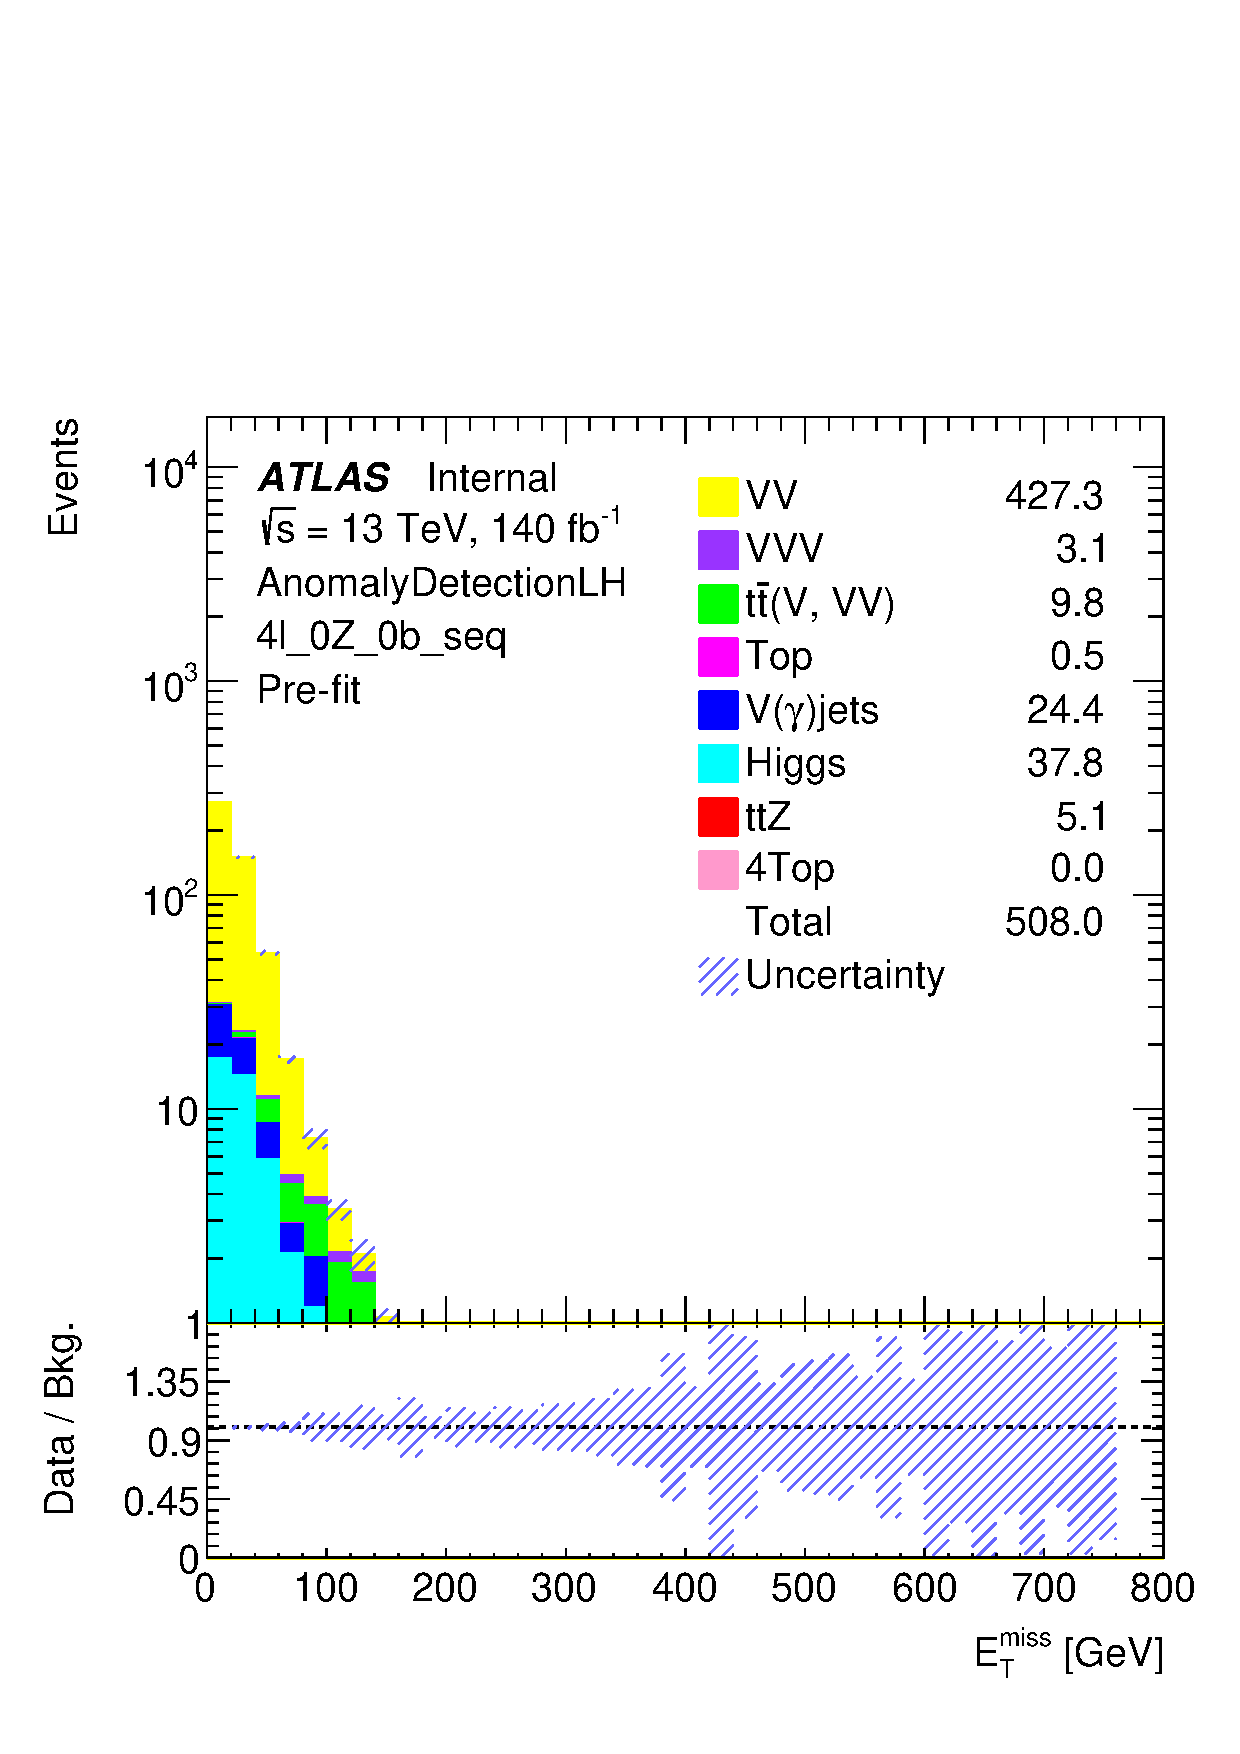
\includegraphics[width=0.24\textwidth]{plots/fourlepLH_run2/Plots/reg_4l_0Z_0b_seq_met.pdf} \\

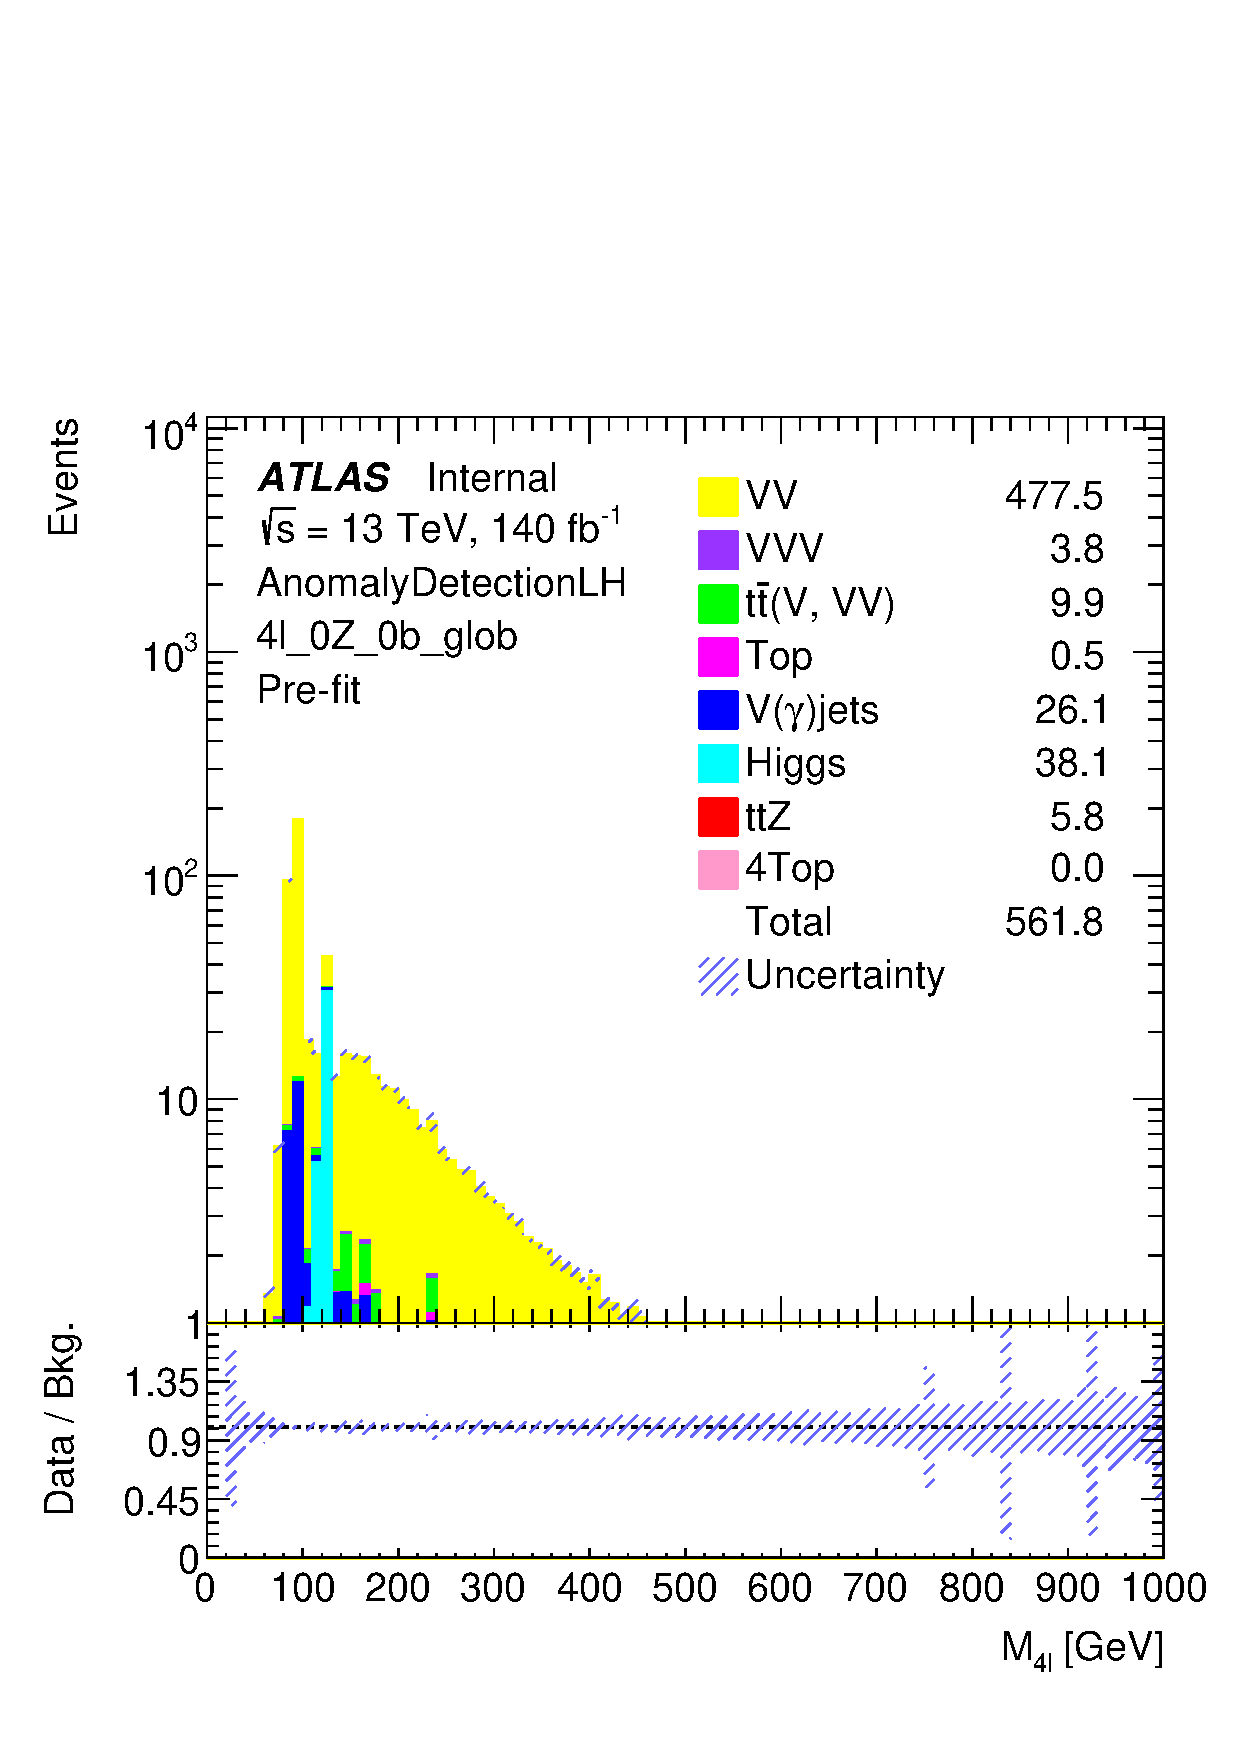
\includegraphics[width=0.24\textwidth]{plots/fourlepLH_run2/Plots/reg_4l_0Z_0b_glob_m4l.pdf} &
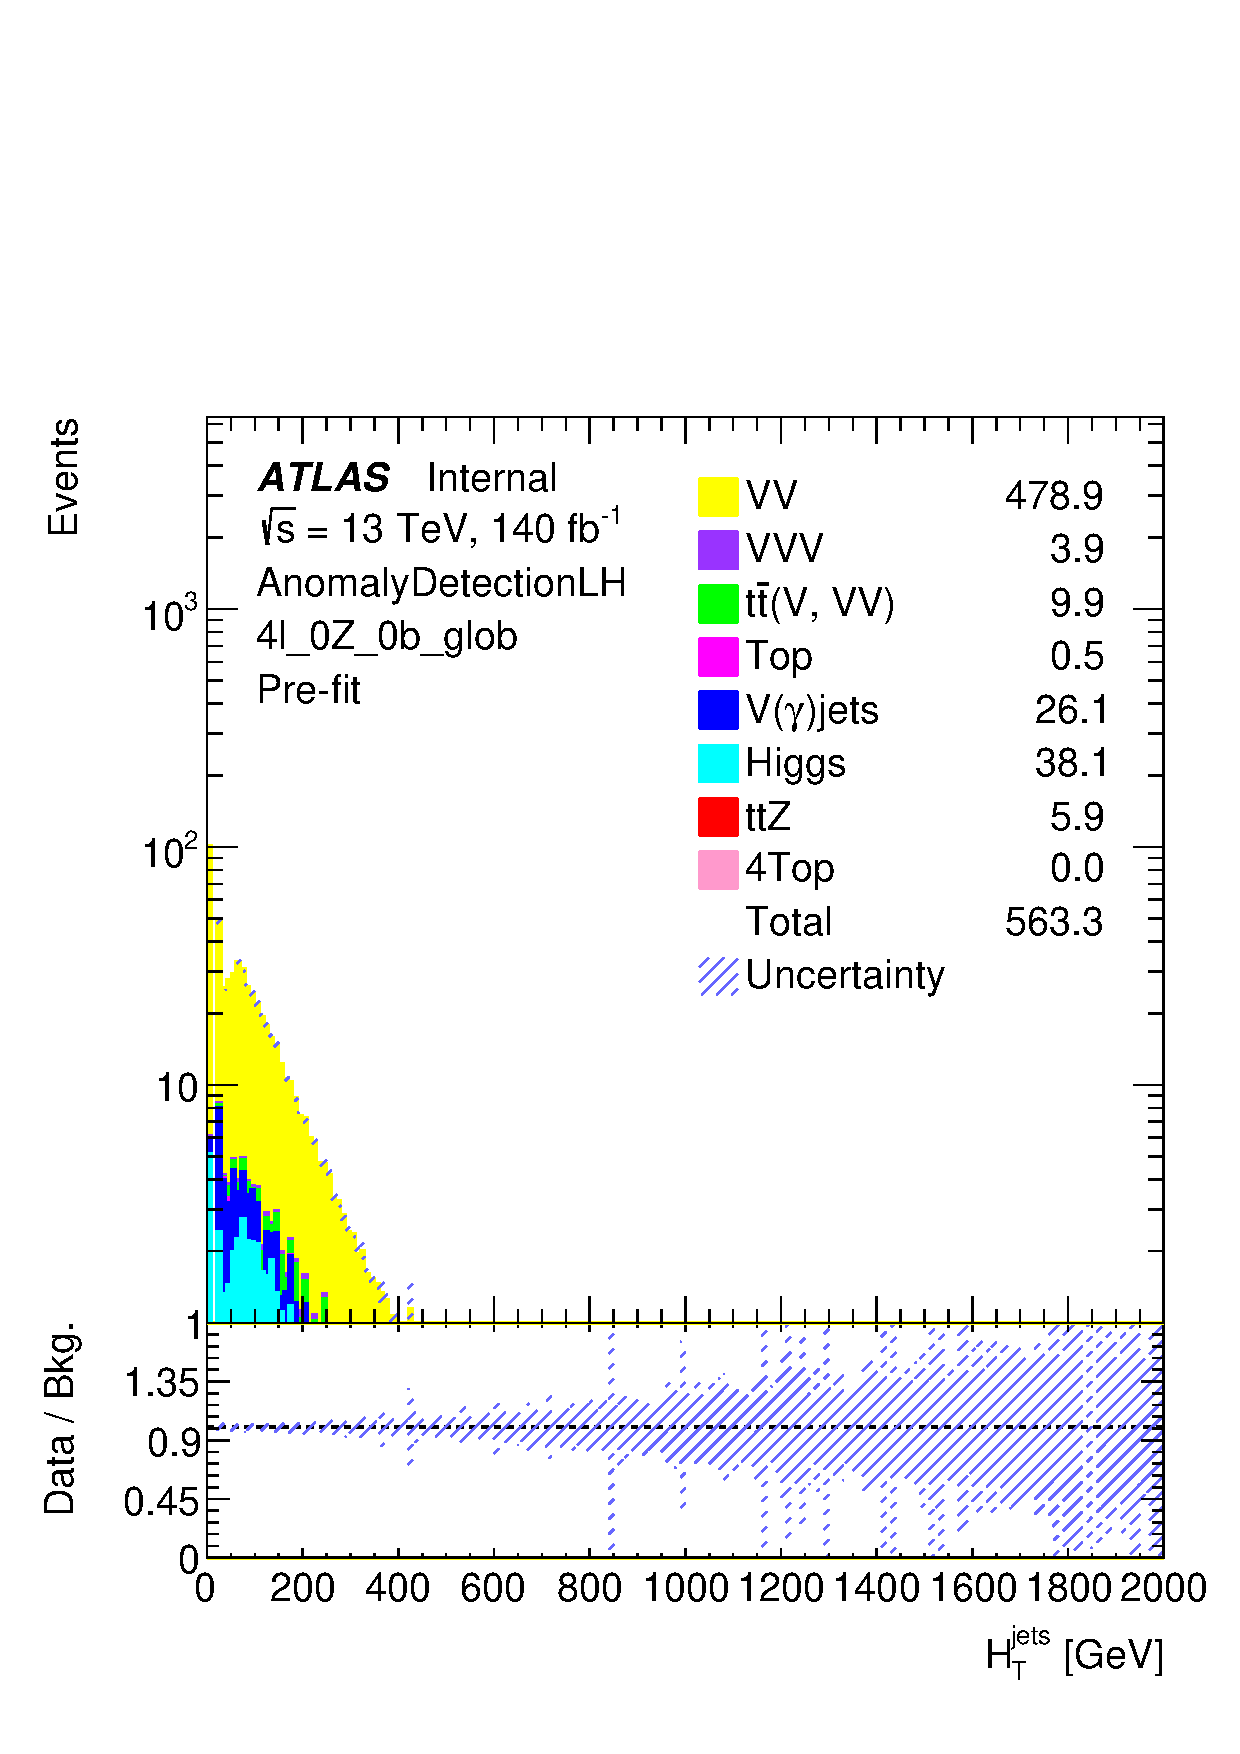
\includegraphics[width=0.24\textwidth]{plots/fourlepLH_run2/Plots/reg_4l_0Z_0b_glob_HT_jets.pdf} &
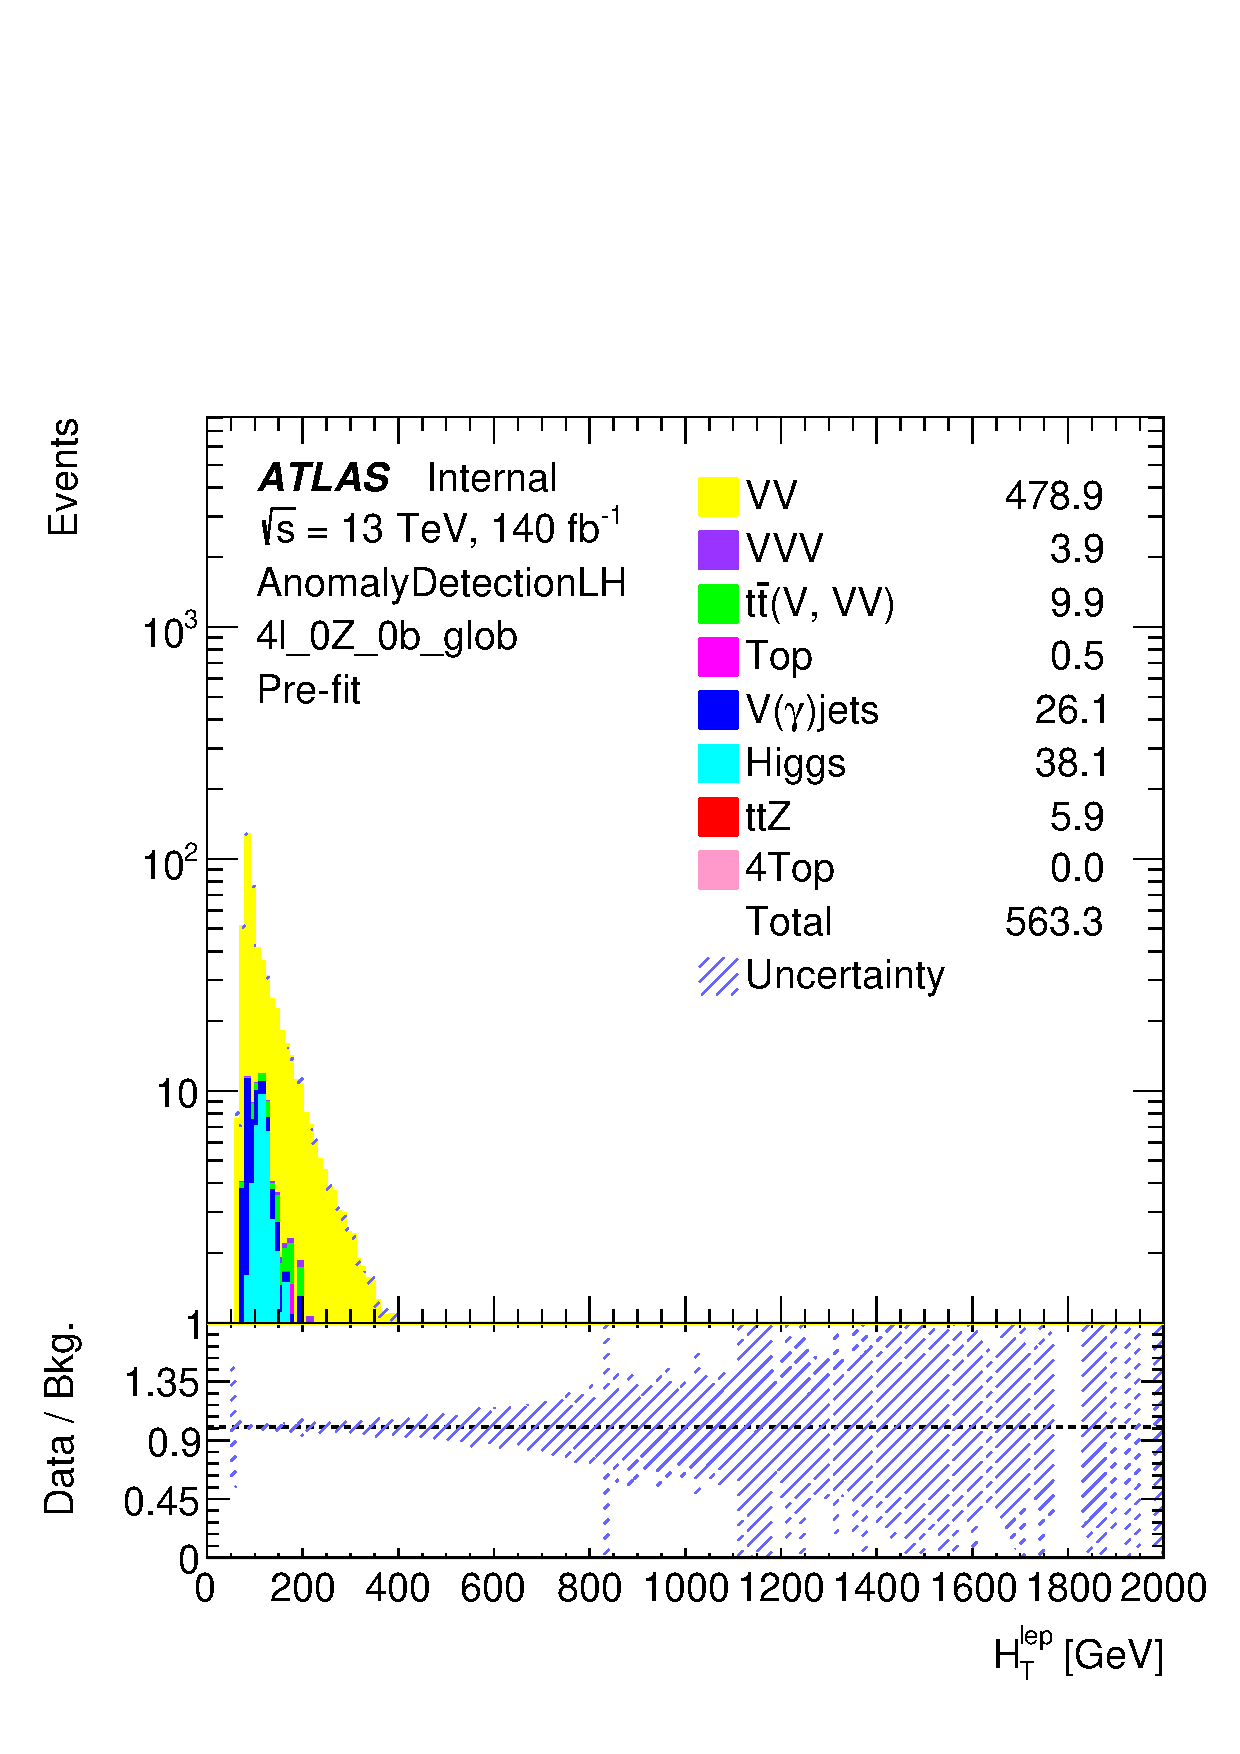
\includegraphics[width=0.24\textwidth]{plots/fourlepLH_run2/Plots/reg_4l_0Z_0b_glob_HT_lep.pdf} &
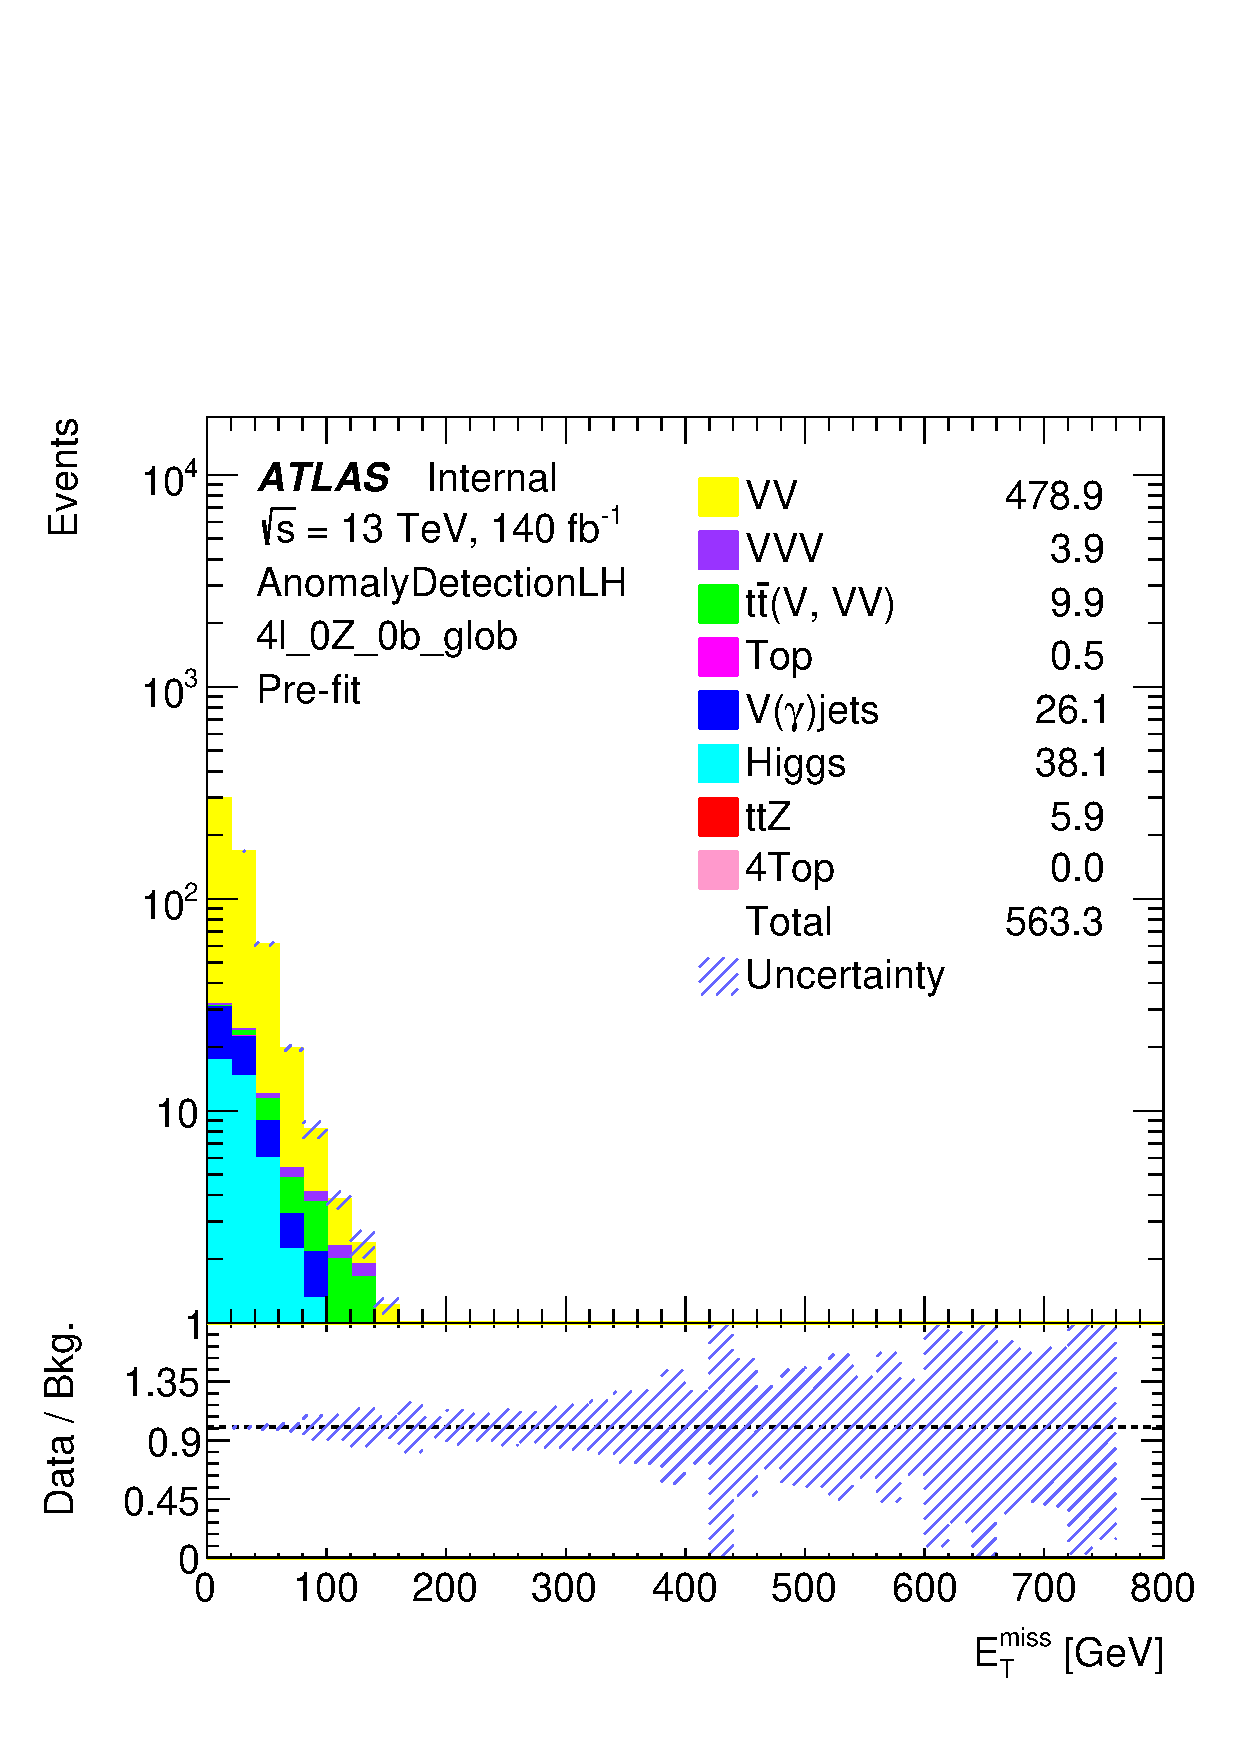
\includegraphics[width=0.24\textwidth]{plots/fourlepLH_run2/Plots/reg_4l_0Z_0b_glob_met.pdf} \\

\end{tabular}
\end{frame}

\begin{frame}{\texttt{Results: 4l\_0Z\_0b}}
\begin{tabular}{cccccc}
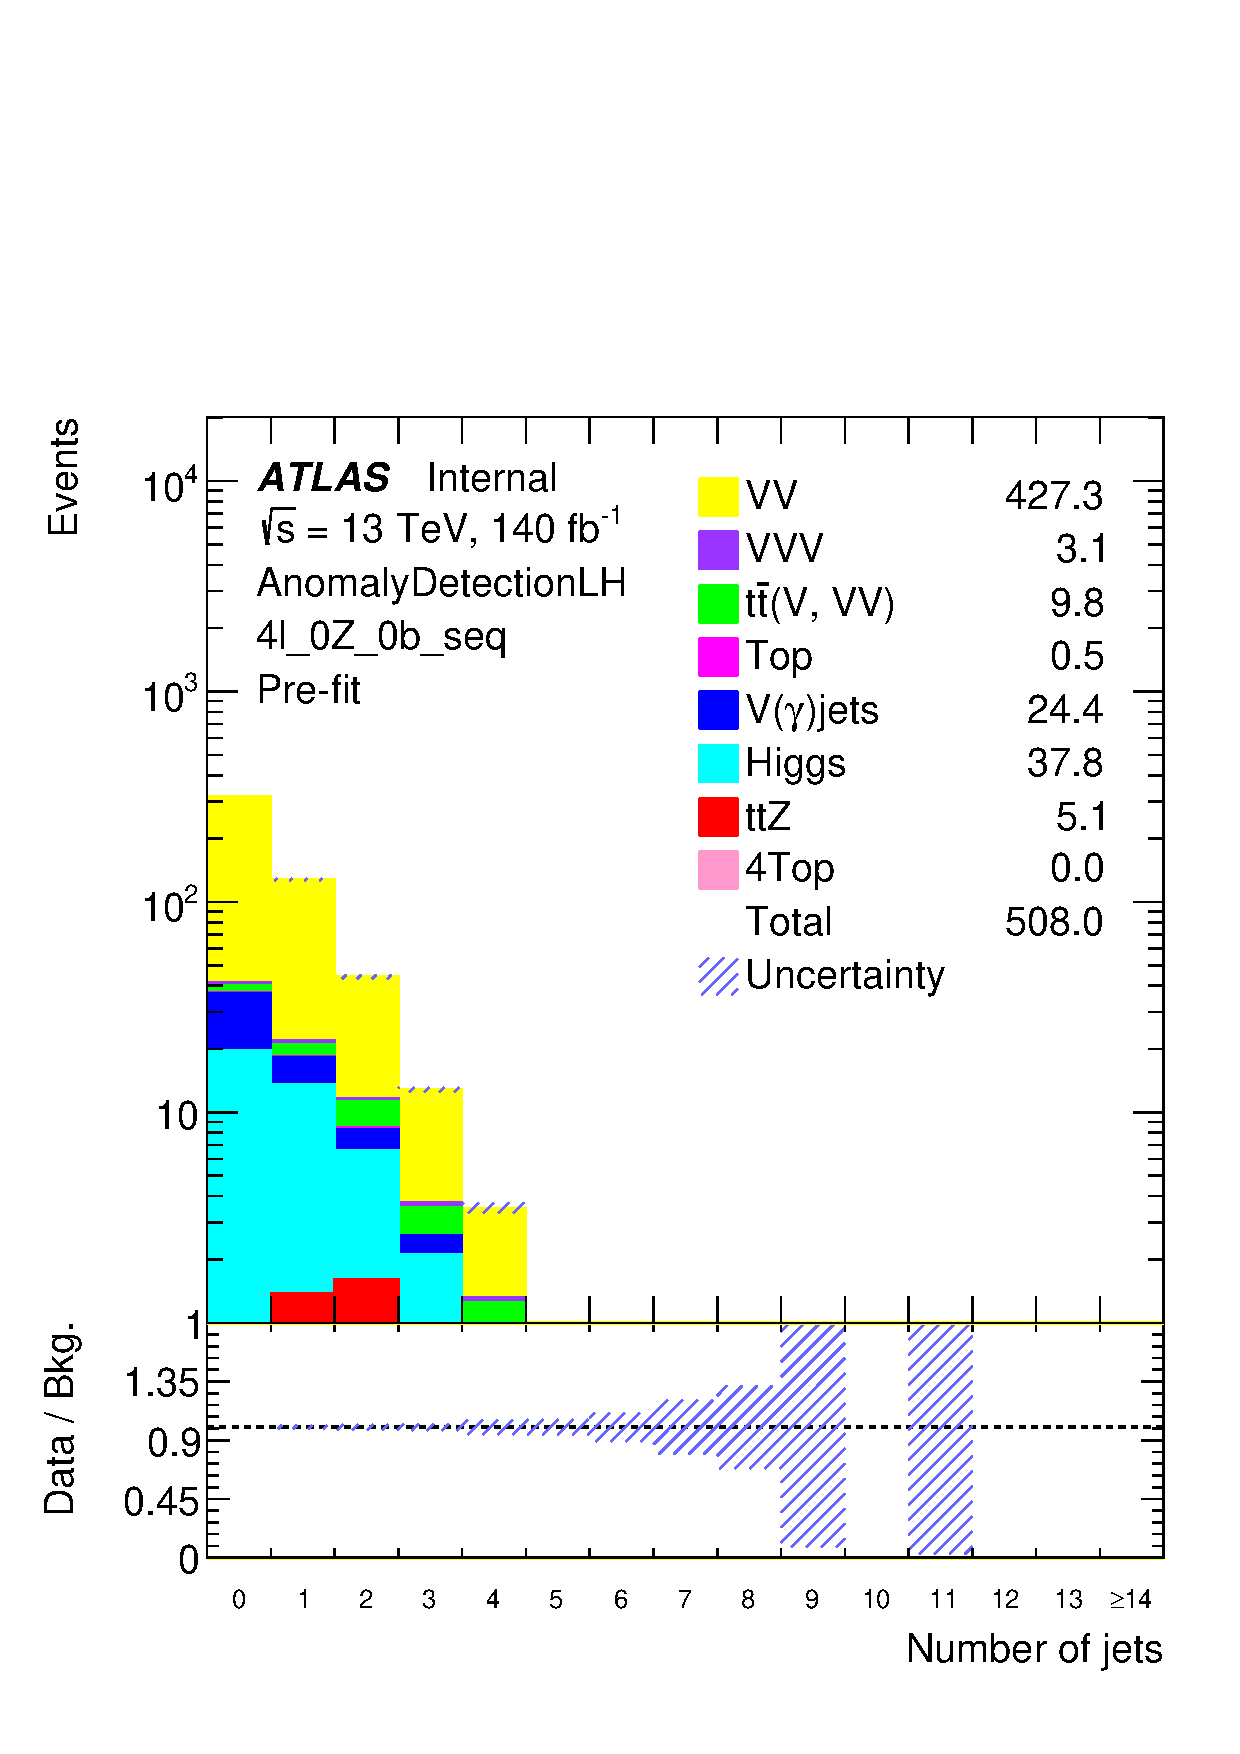
\includegraphics[width=0.24\textwidth]{plots/fourlepLH_run2/Plots/reg_4l_0Z_0b_seq_nJets.pdf} &
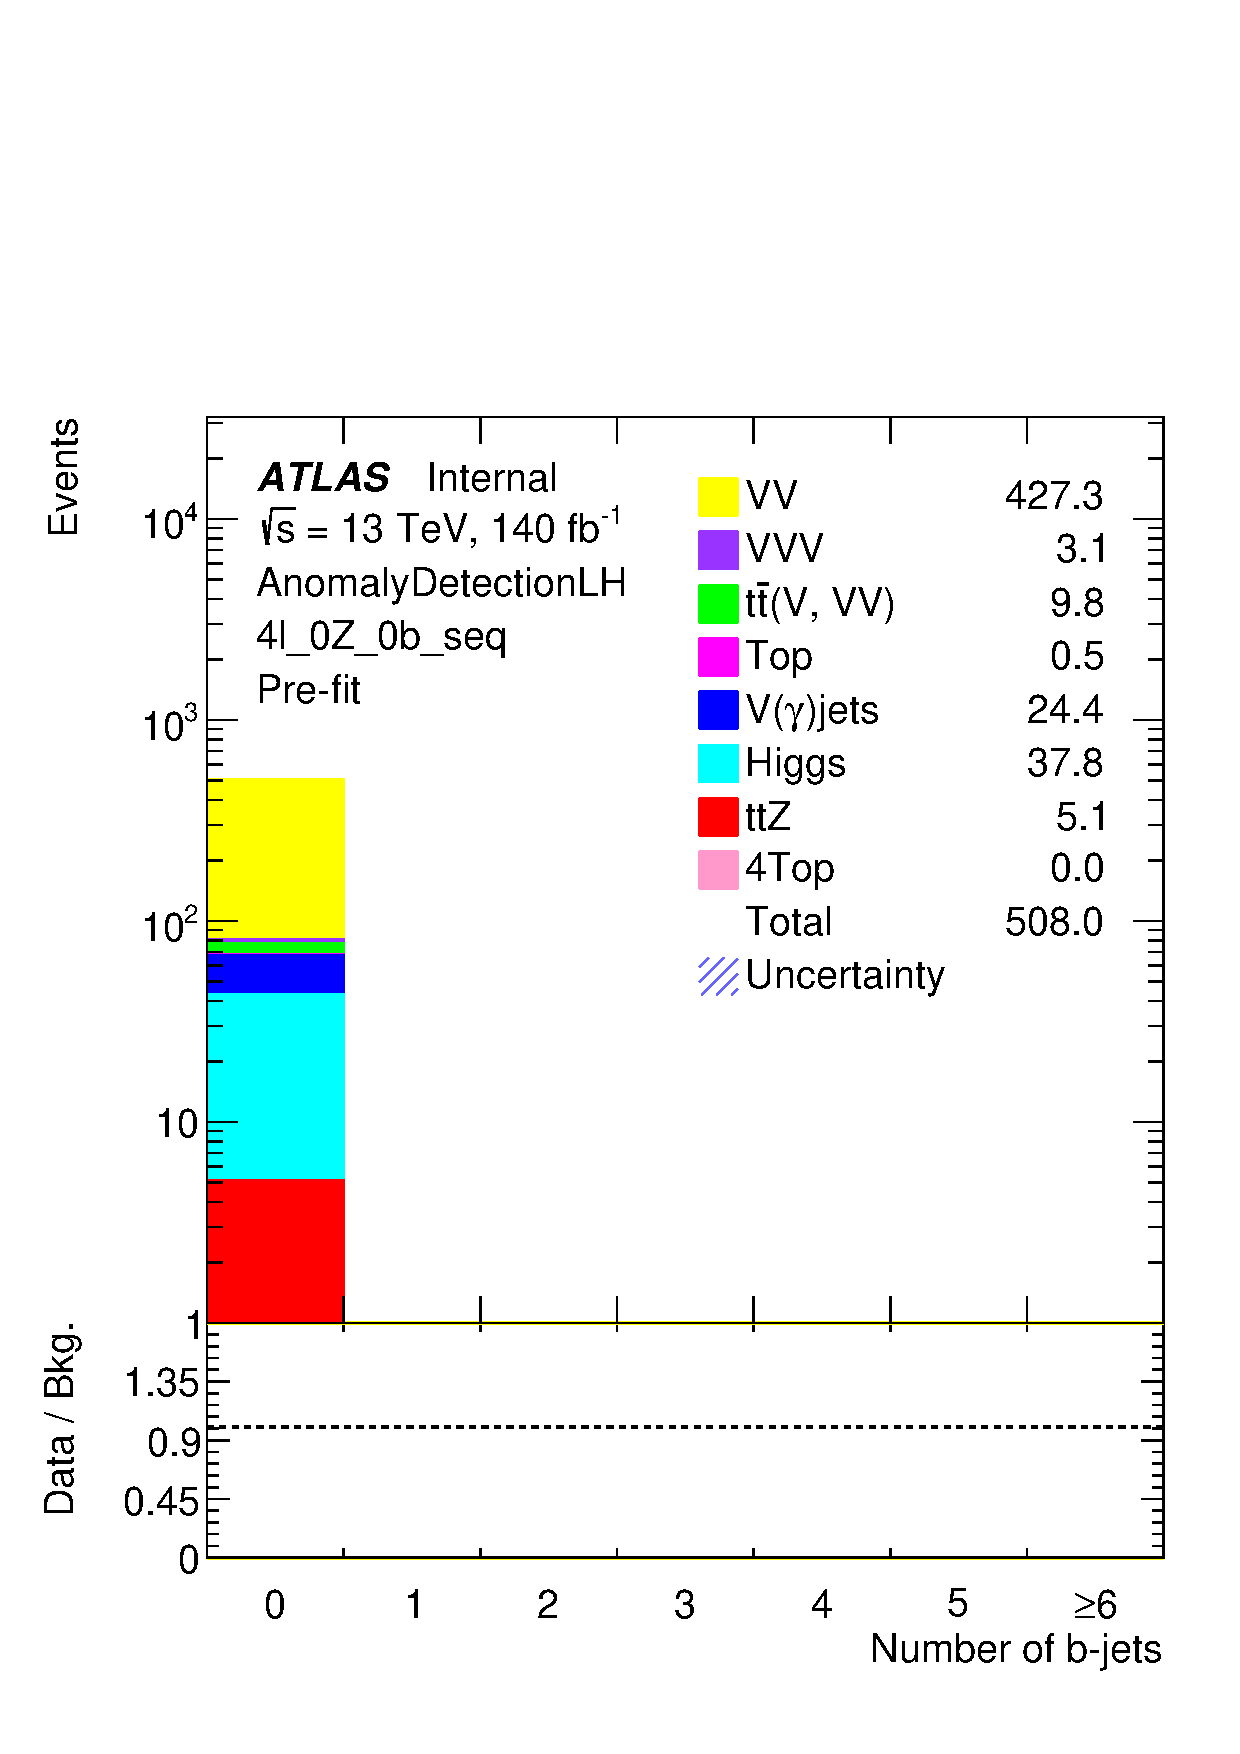
\includegraphics[width=0.24\textwidth]{plots/fourlepLH_run2/Plots/reg_4l_0Z_0b_seq_nbJets.pdf} &
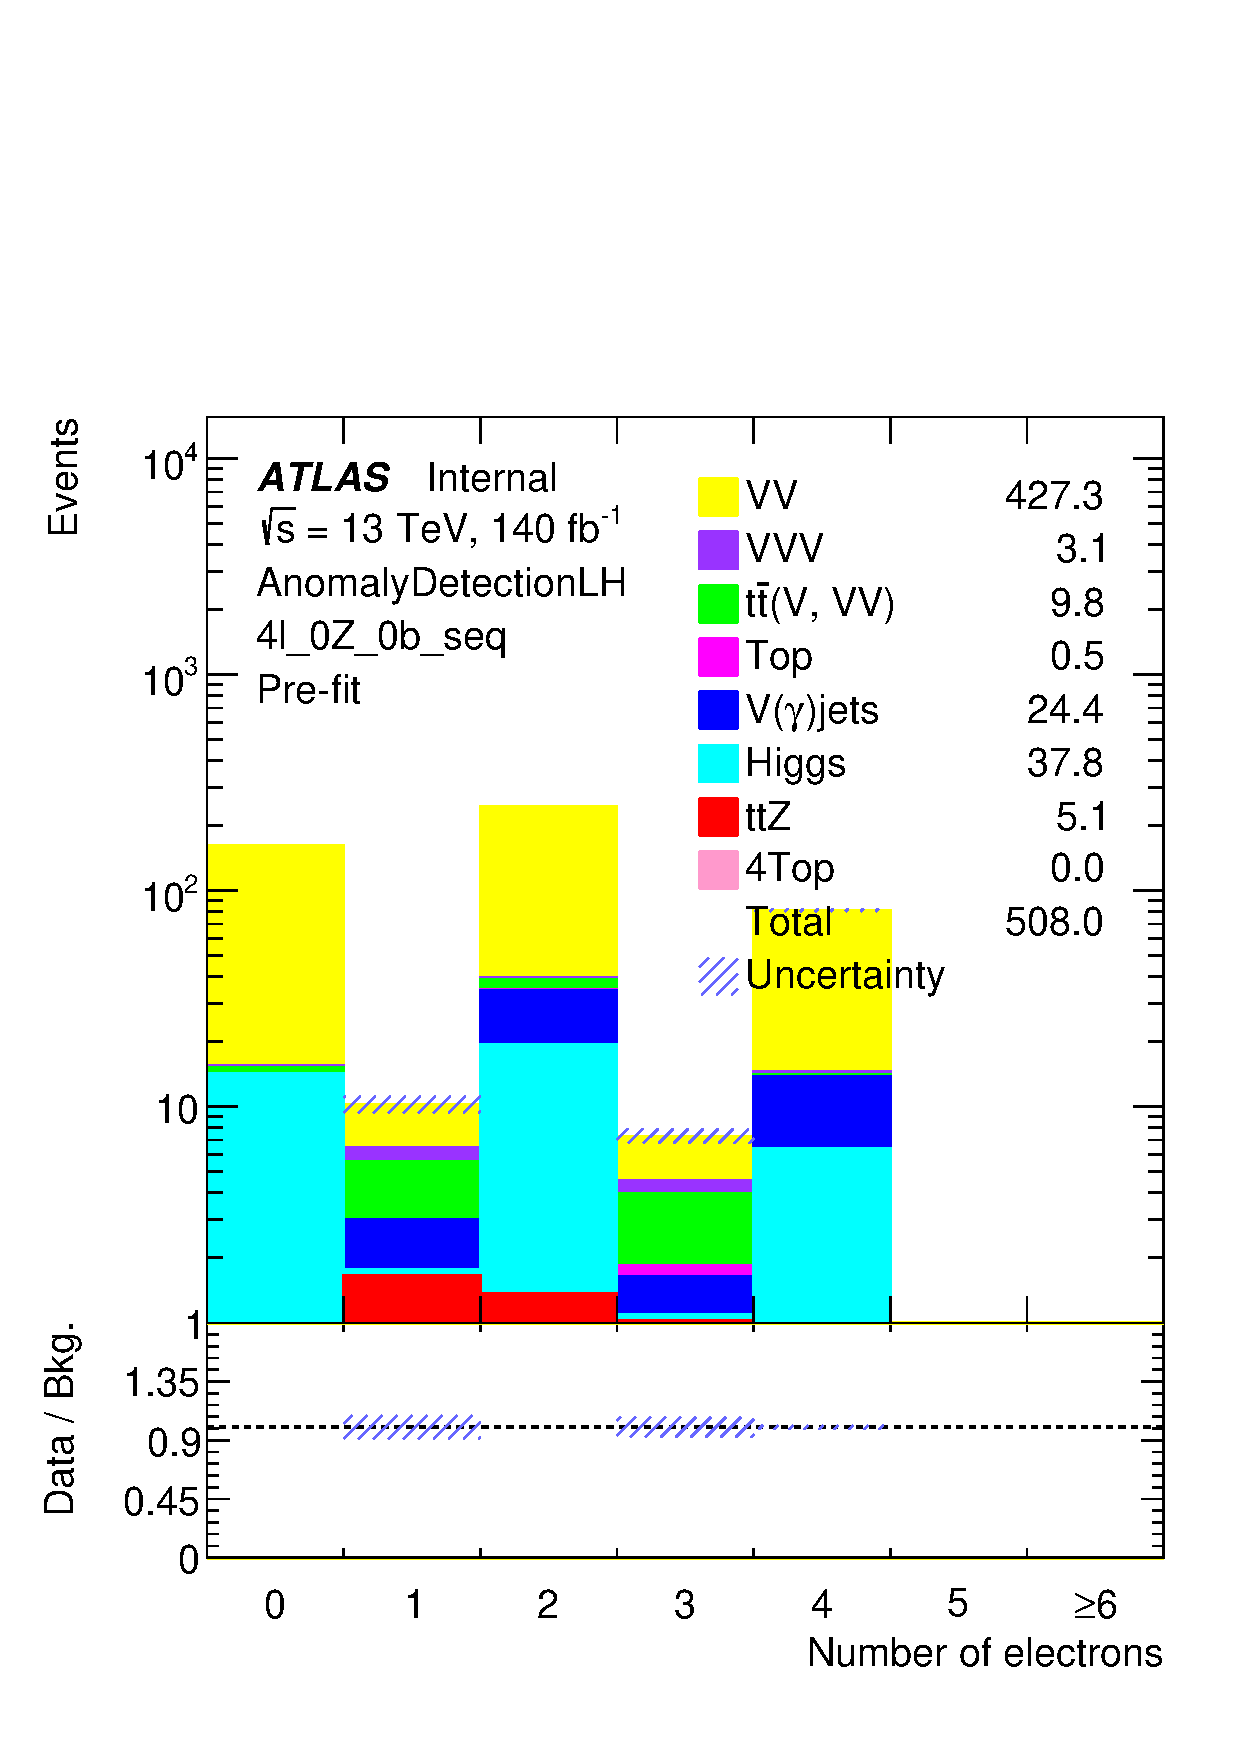
\includegraphics[width=0.24\textwidth]{plots/fourlepLH_run2/Plots/reg_4l_0Z_0b_seq_nElectrons.pdf} &
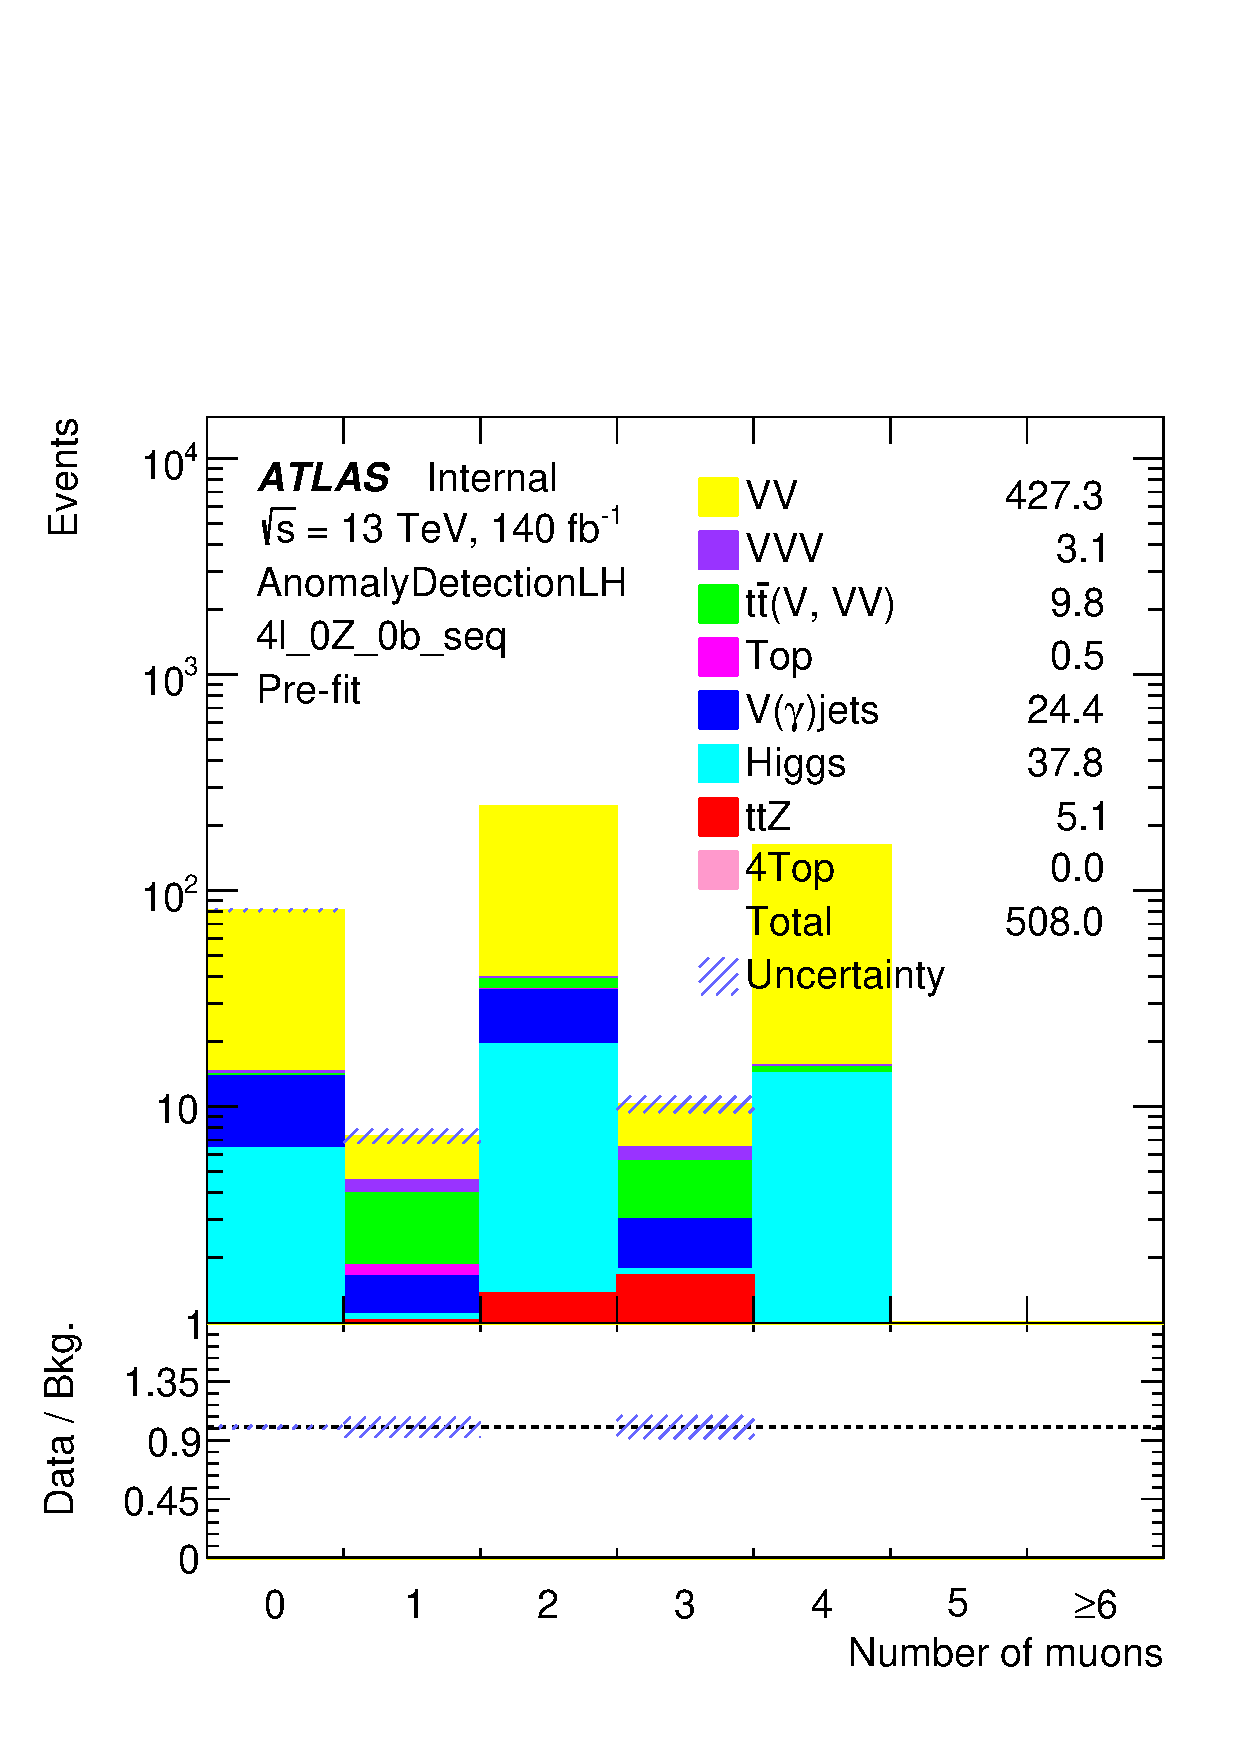
\includegraphics[width=0.24\textwidth]{plots/fourlepLH_run2/Plots/reg_4l_0Z_0b_seq_nMuons.pdf} \\

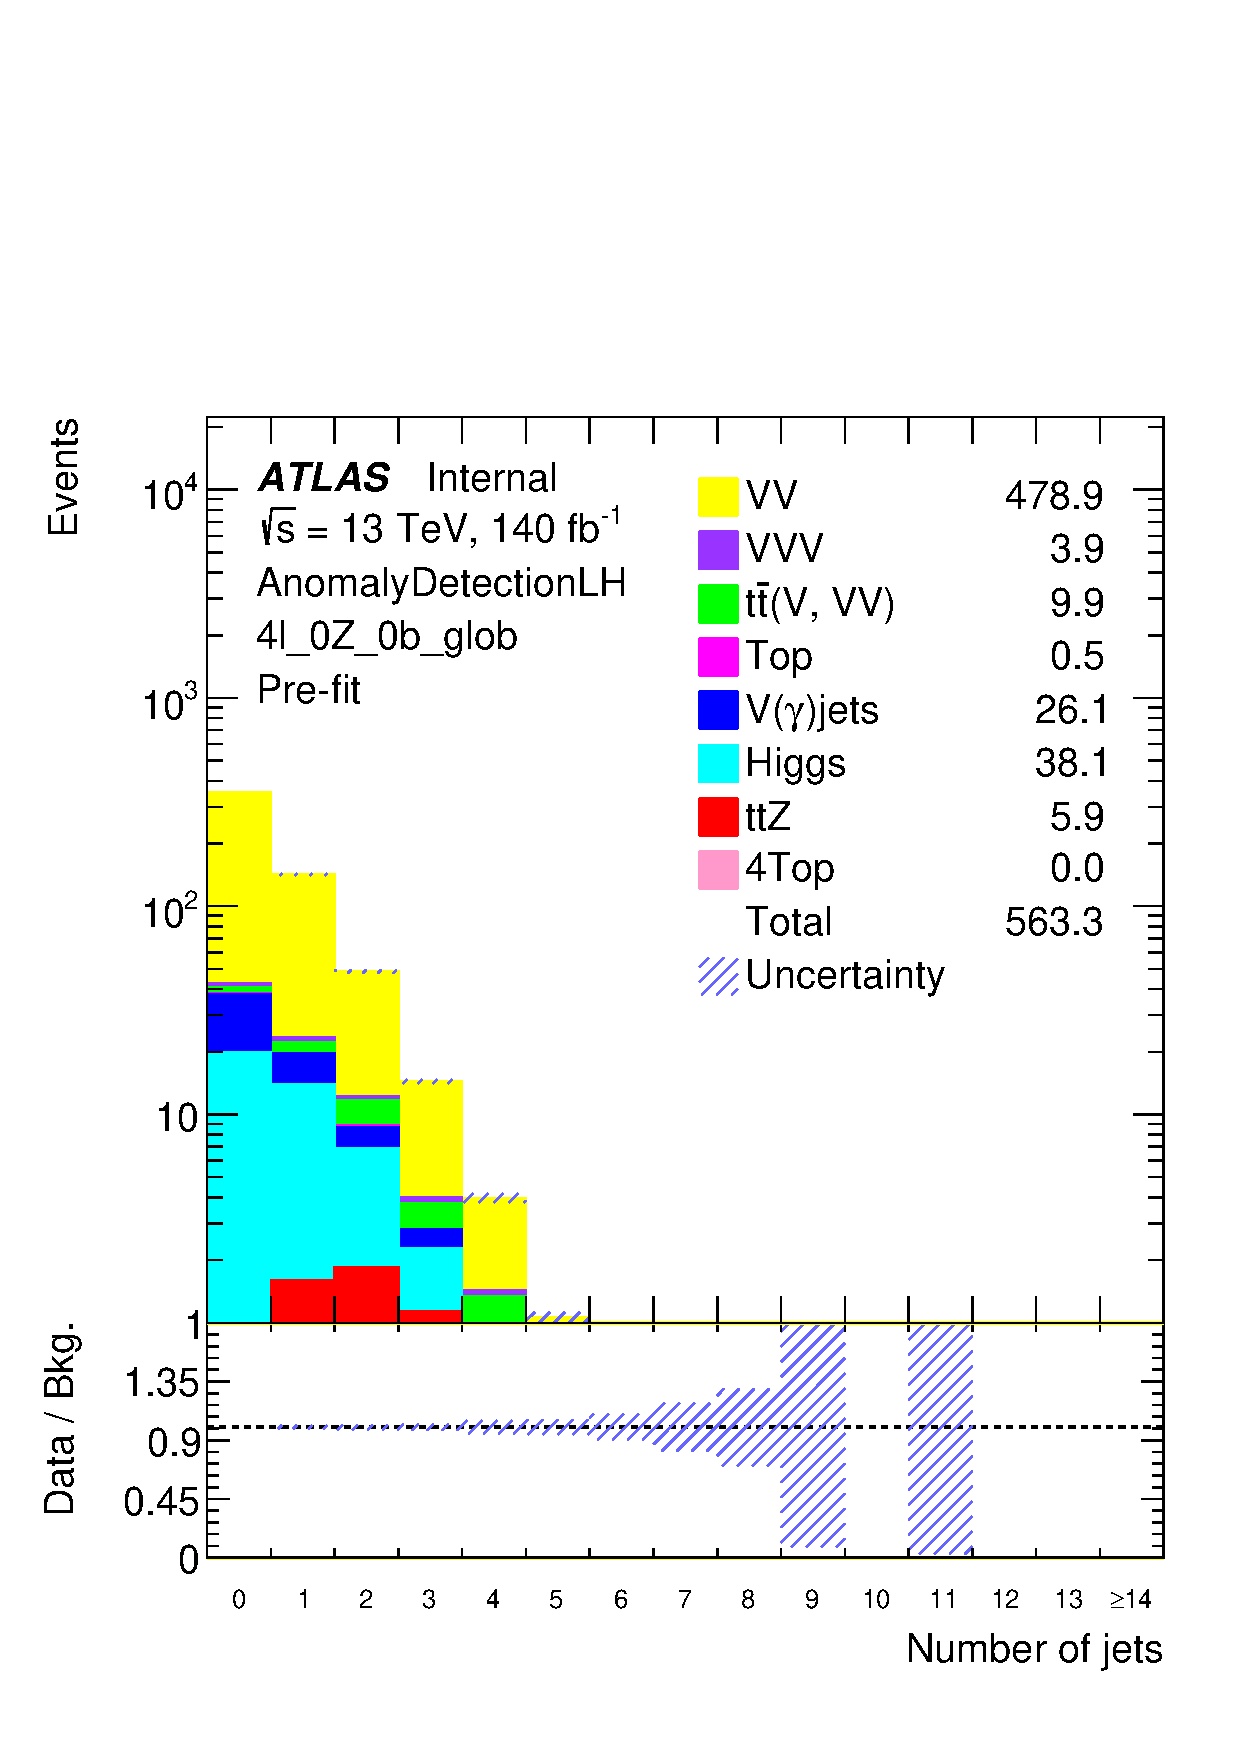
\includegraphics[width=0.24\textwidth]{plots/fourlepLH_run2/Plots/reg_4l_0Z_0b_glob_nJets.pdf} &
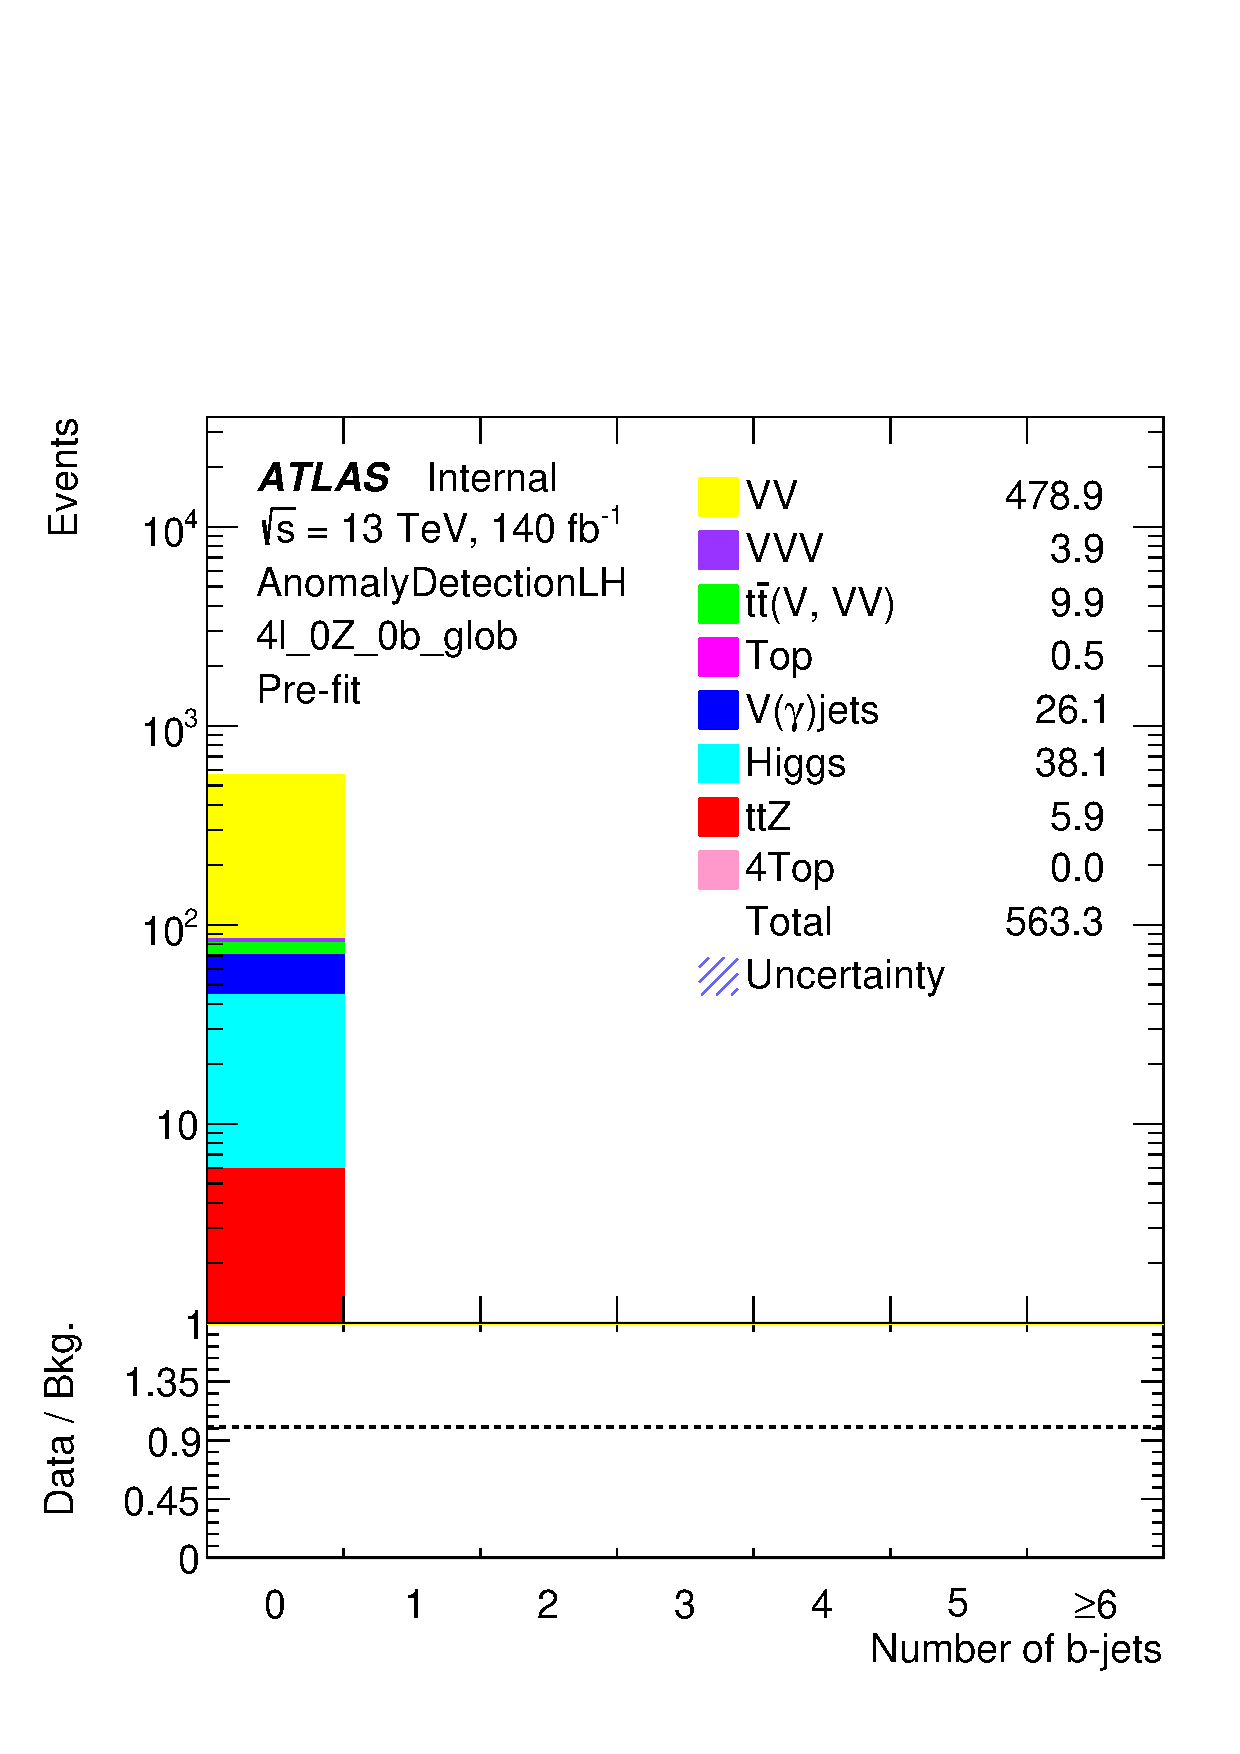
\includegraphics[width=0.24\textwidth]{plots/fourlepLH_run2/Plots/reg_4l_0Z_0b_glob_nbJets.pdf} &
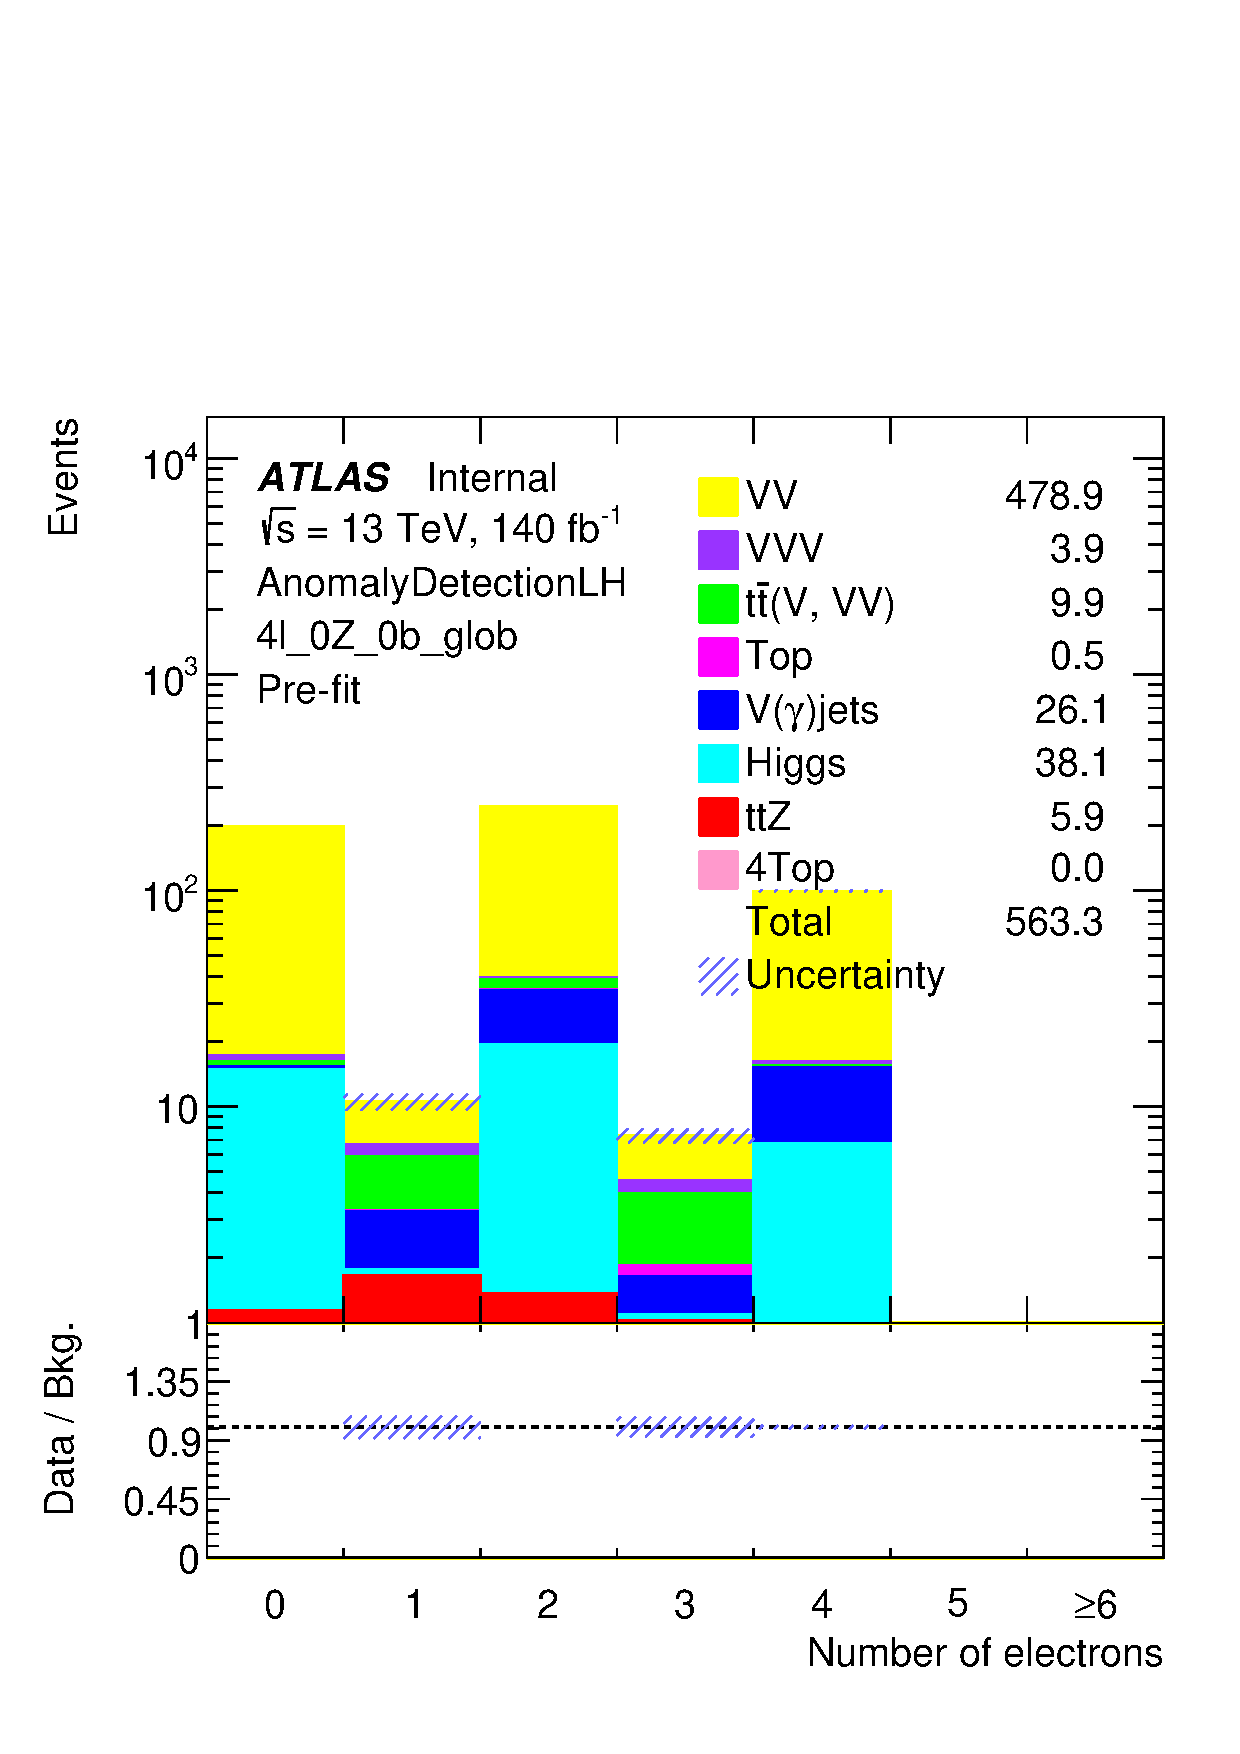
\includegraphics[width=0.24\textwidth]{plots/fourlepLH_run2/Plots/reg_4l_0Z_0b_glob_nElectrons.pdf} &
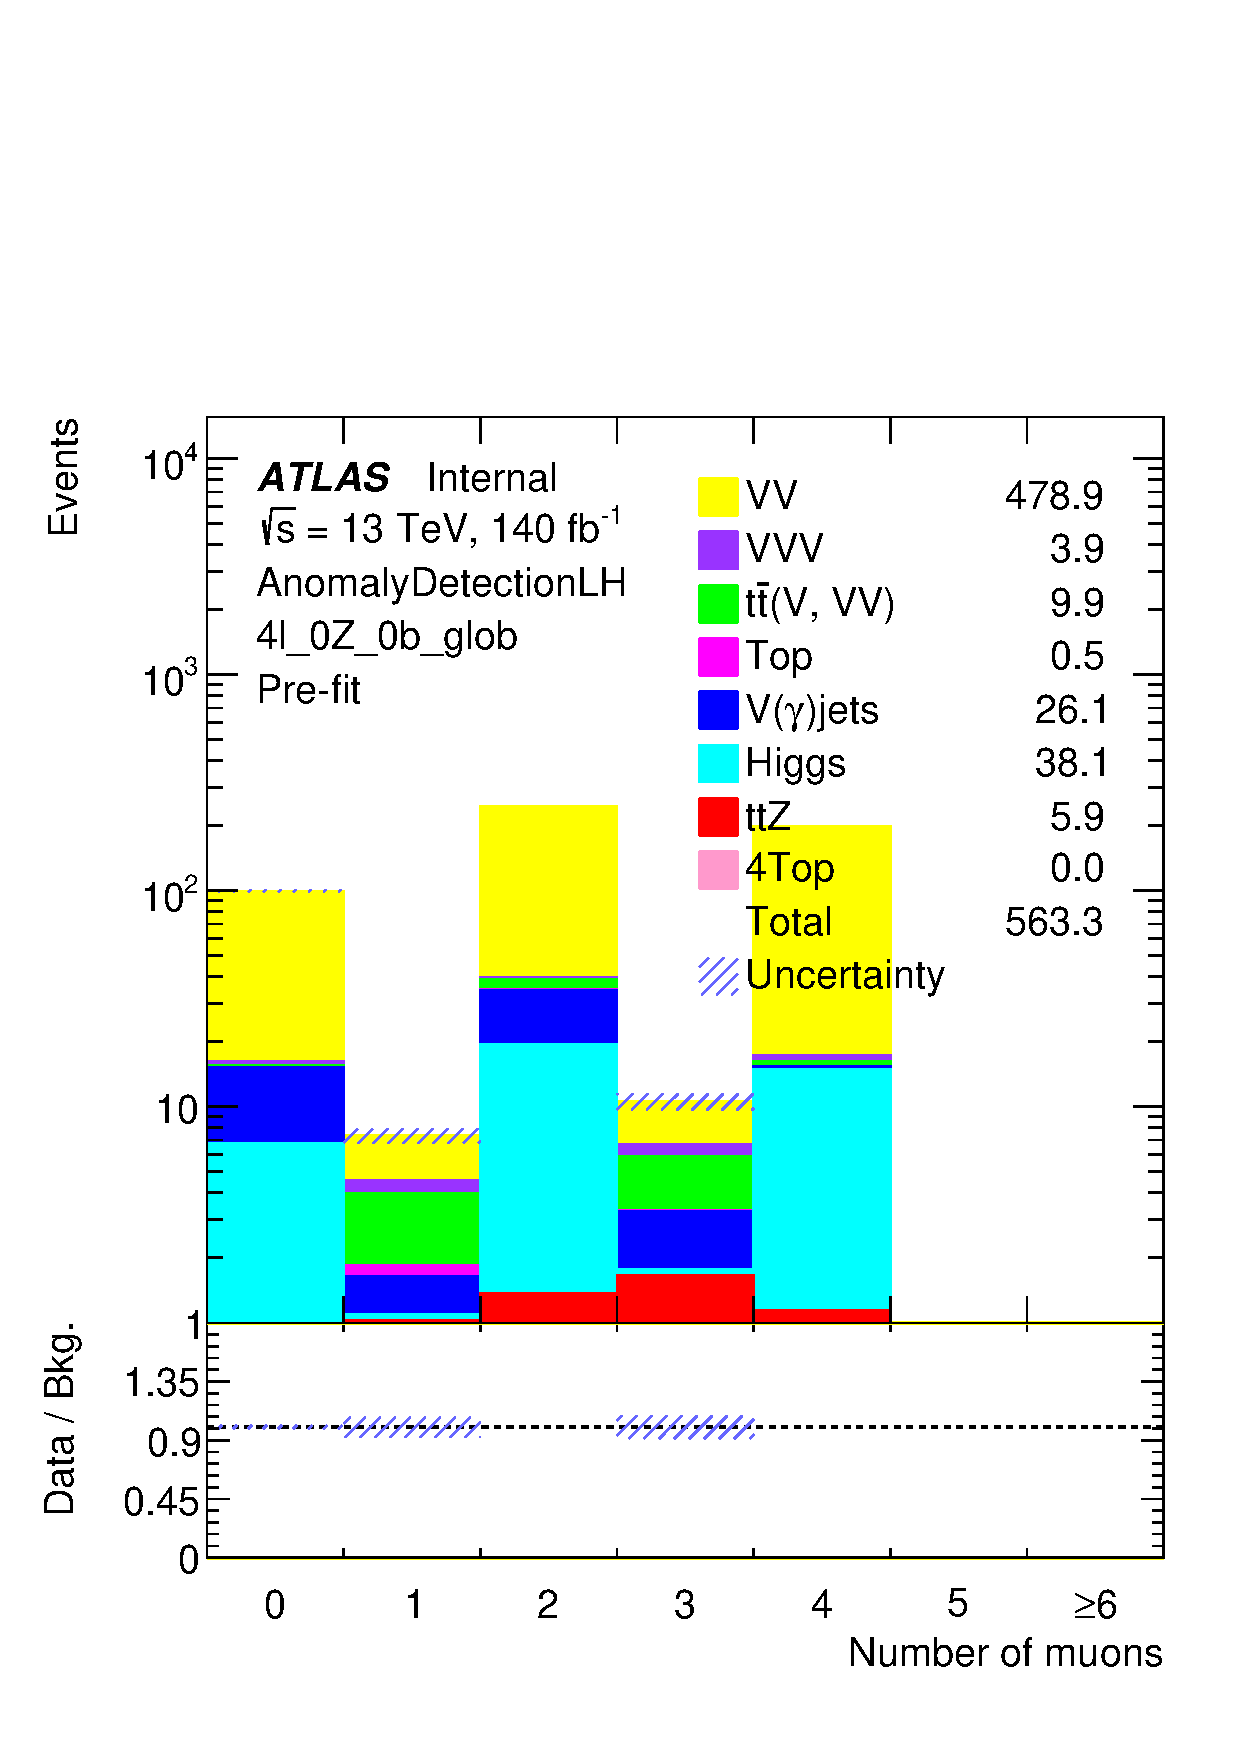
\includegraphics[width=0.24\textwidth]{plots/fourlepLH_run2/Plots/reg_4l_0Z_0b_glob_nMuons.pdf} \\

\end{tabular}
\end{frame}

\begin{frame}{\texttt{Results: 4l\_0Z\_0b}}
\begin{tabular}{cccccc}
\includegraphics[width=0.24\textwidth]{plots/fourlepLH_run2/Plots/reg_4l_0Z_0b_seq_lep_pt_0.pdf} &
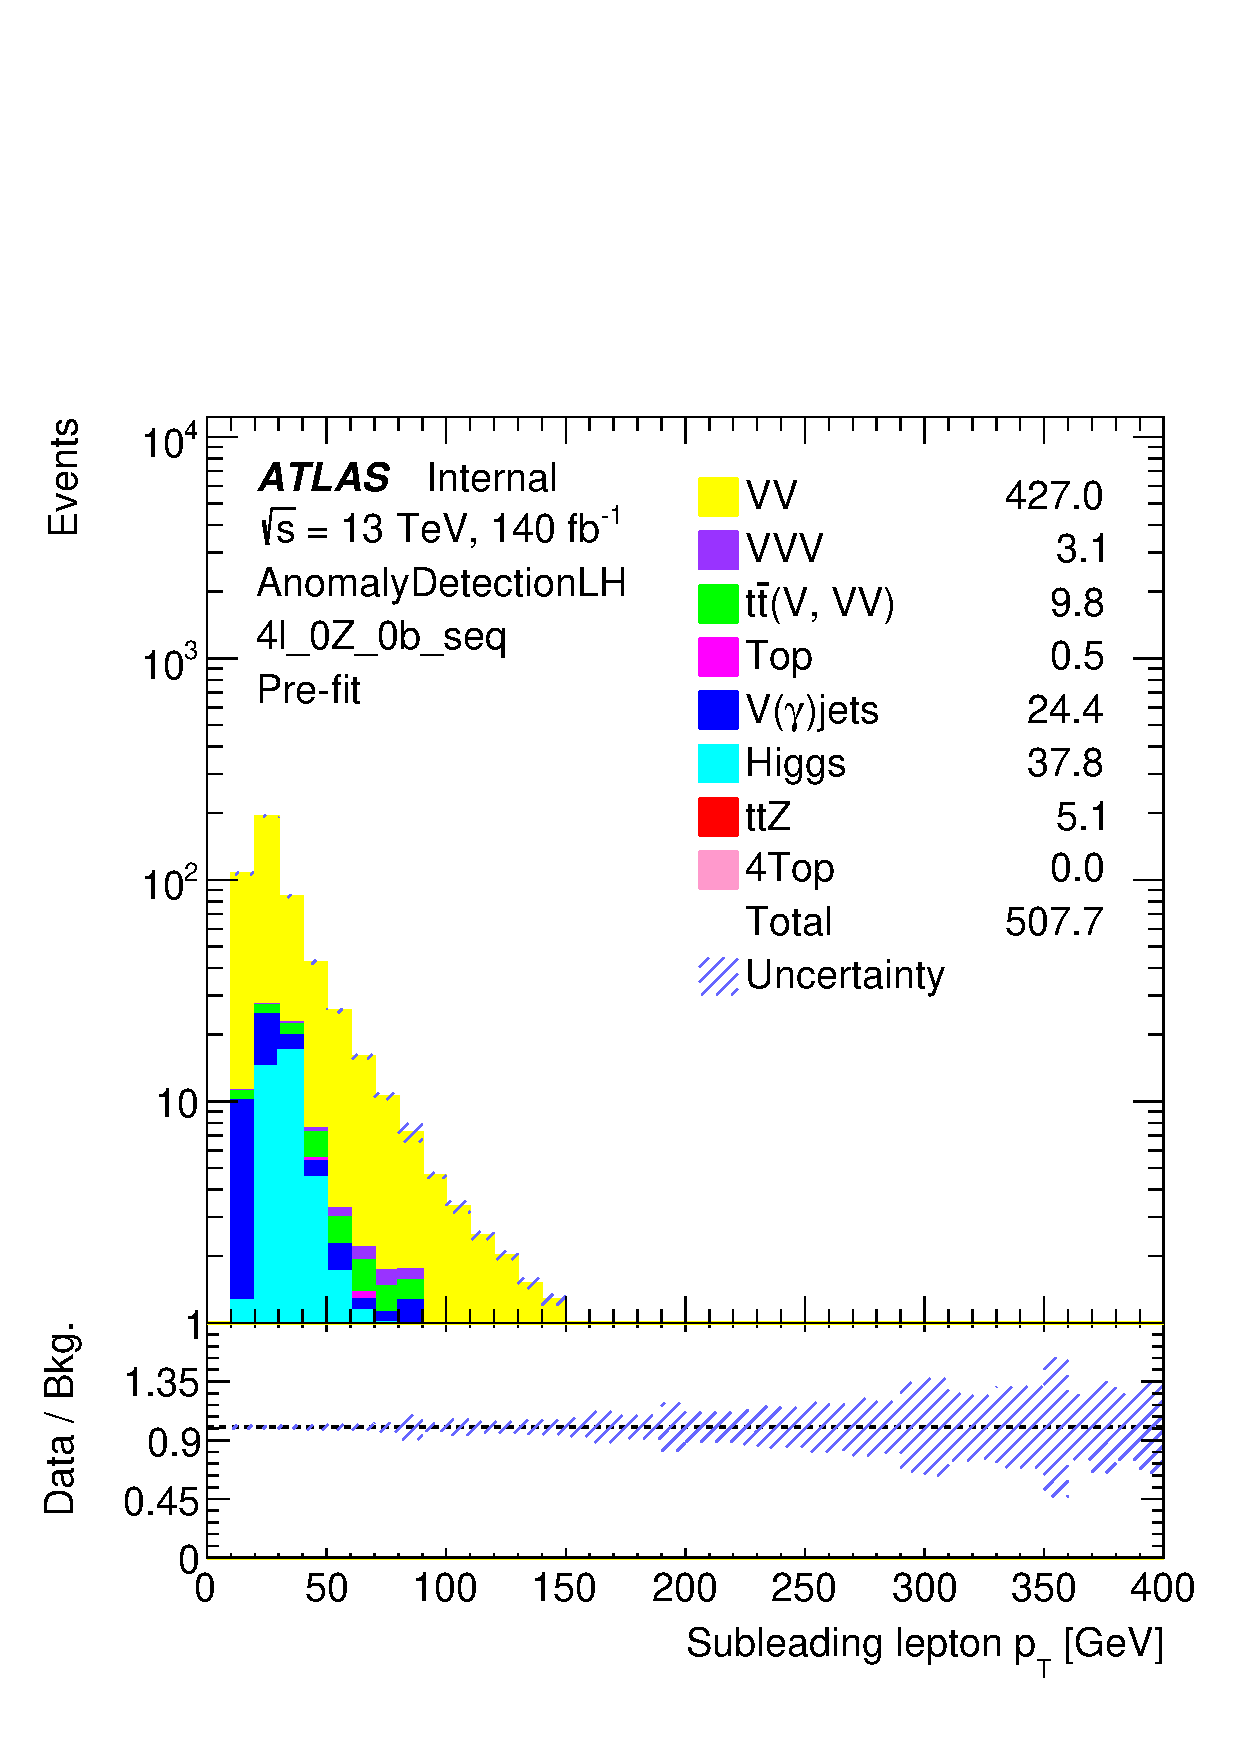
\includegraphics[width=0.24\textwidth]{plots/fourlepLH_run2/Plots/reg_4l_0Z_0b_seq_lep_pt_1.pdf} &
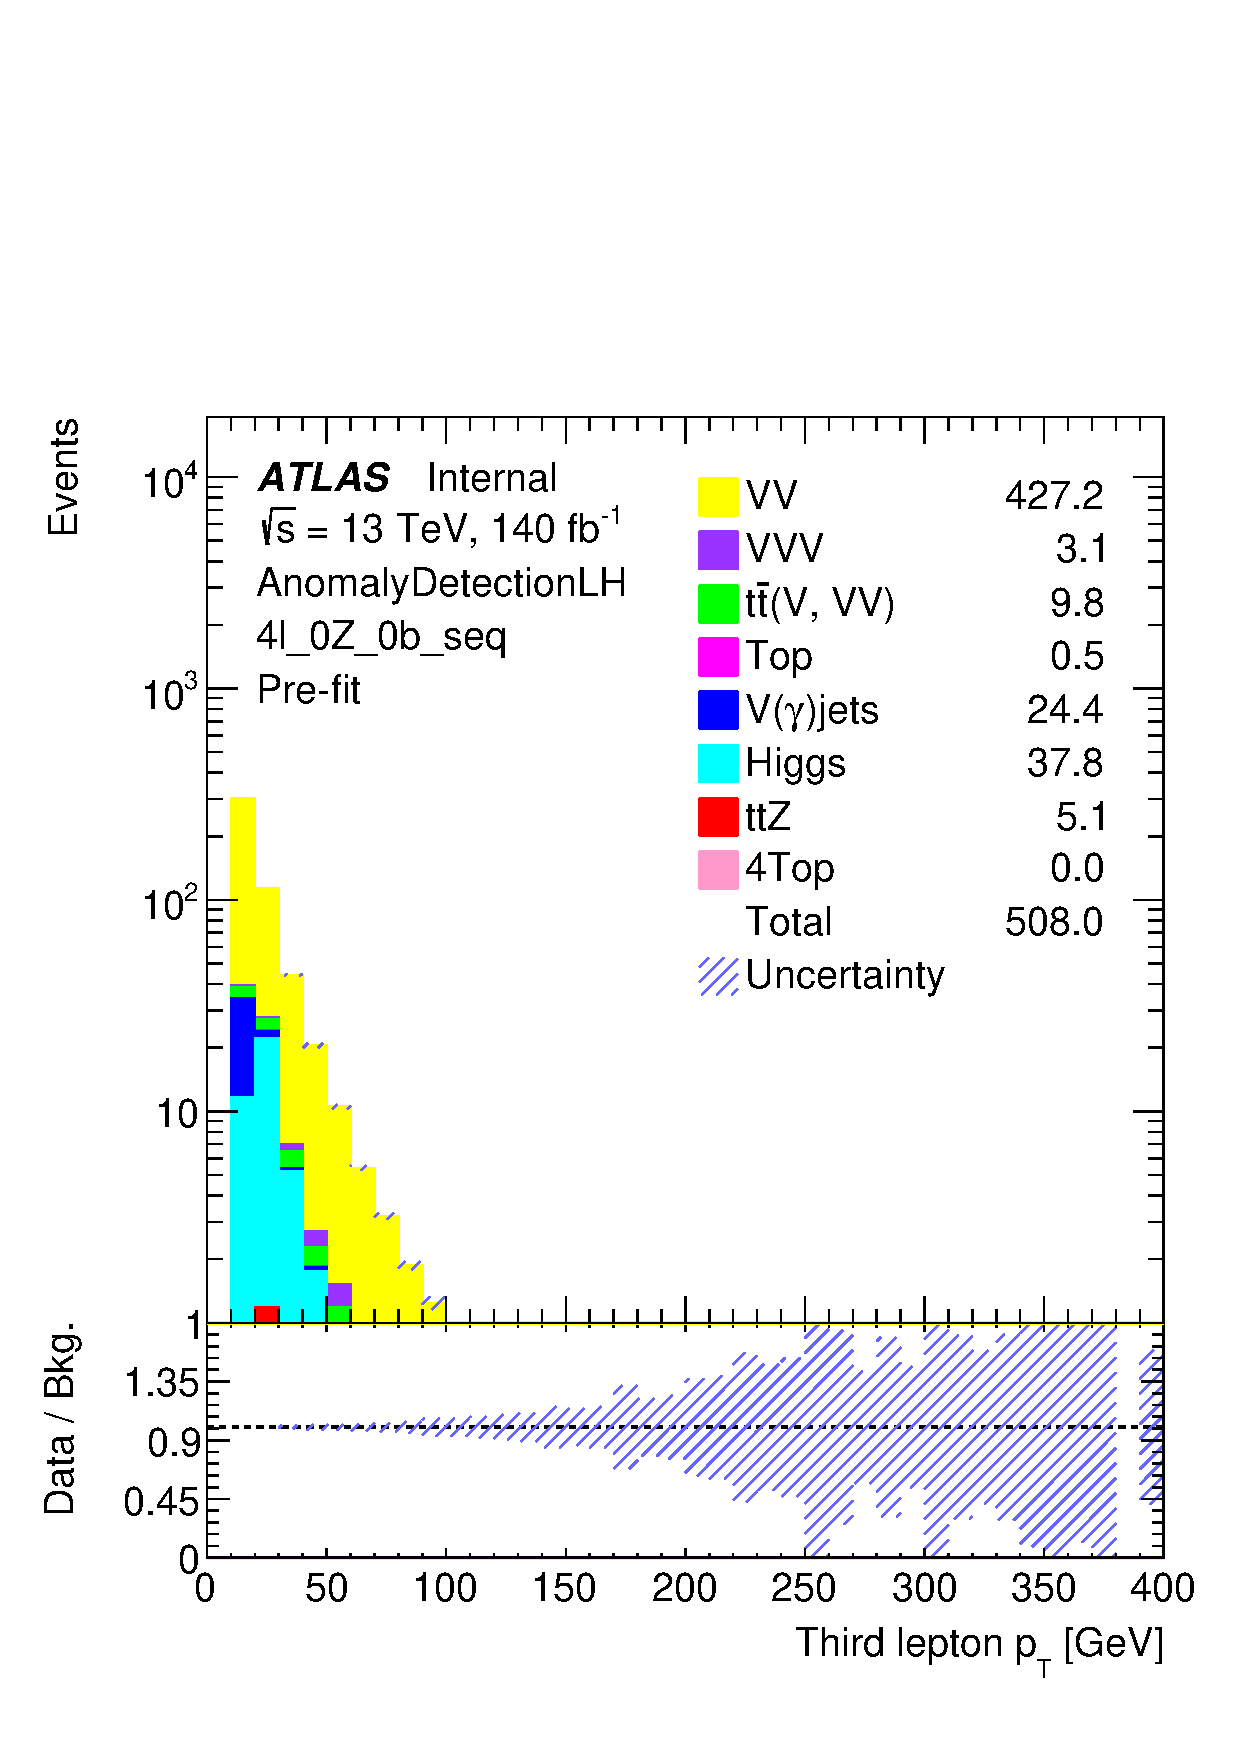
\includegraphics[width=0.24\textwidth]{plots/fourlepLH_run2/Plots/reg_4l_0Z_0b_seq_lep_pt_2.pdf} &
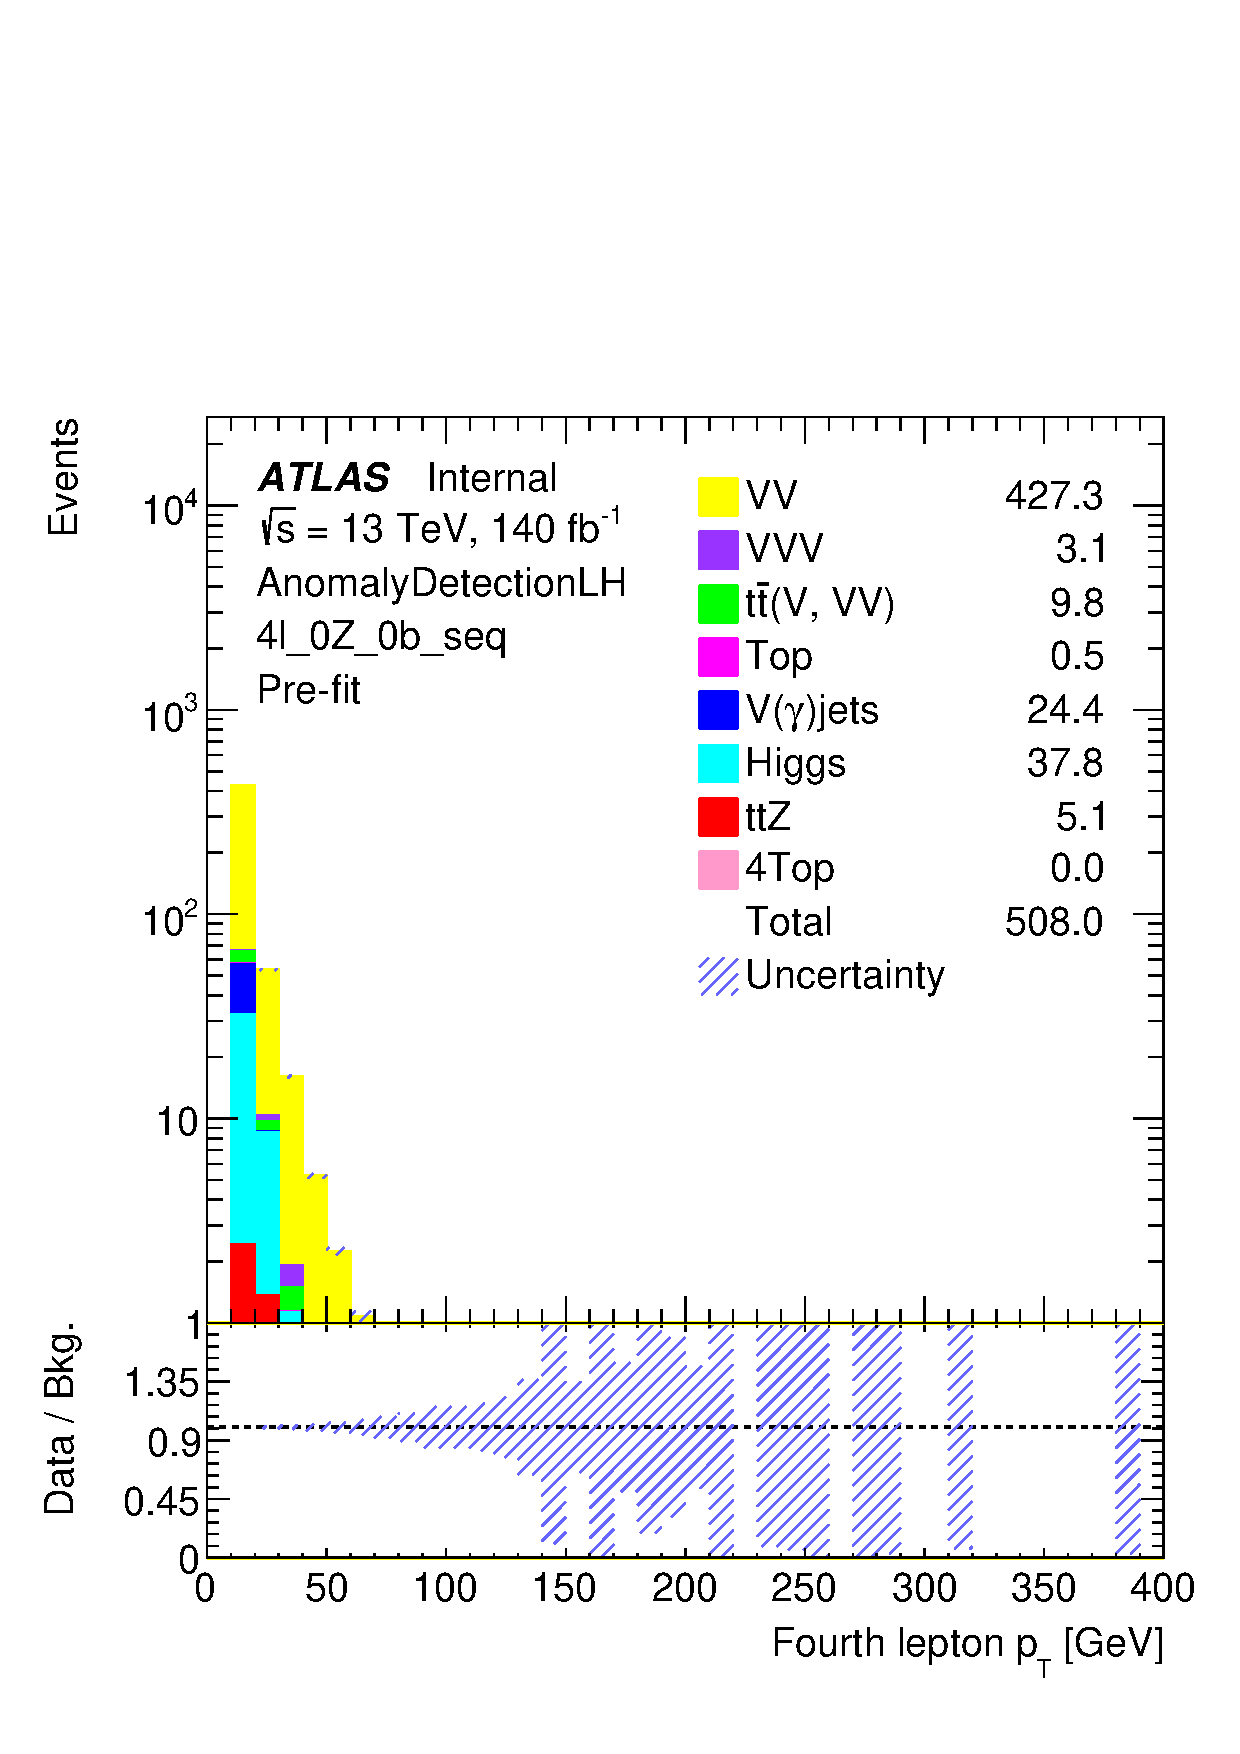
\includegraphics[width=0.24\textwidth]{plots/fourlepLH_run2/Plots/reg_4l_0Z_0b_seq_lep_pt_3.pdf} \\

\includegraphics[width=0.24\textwidth]{plots/fourlepLH_run2/Plots/reg_4l_0Z_0b_glob_lep_pt_0.pdf} &
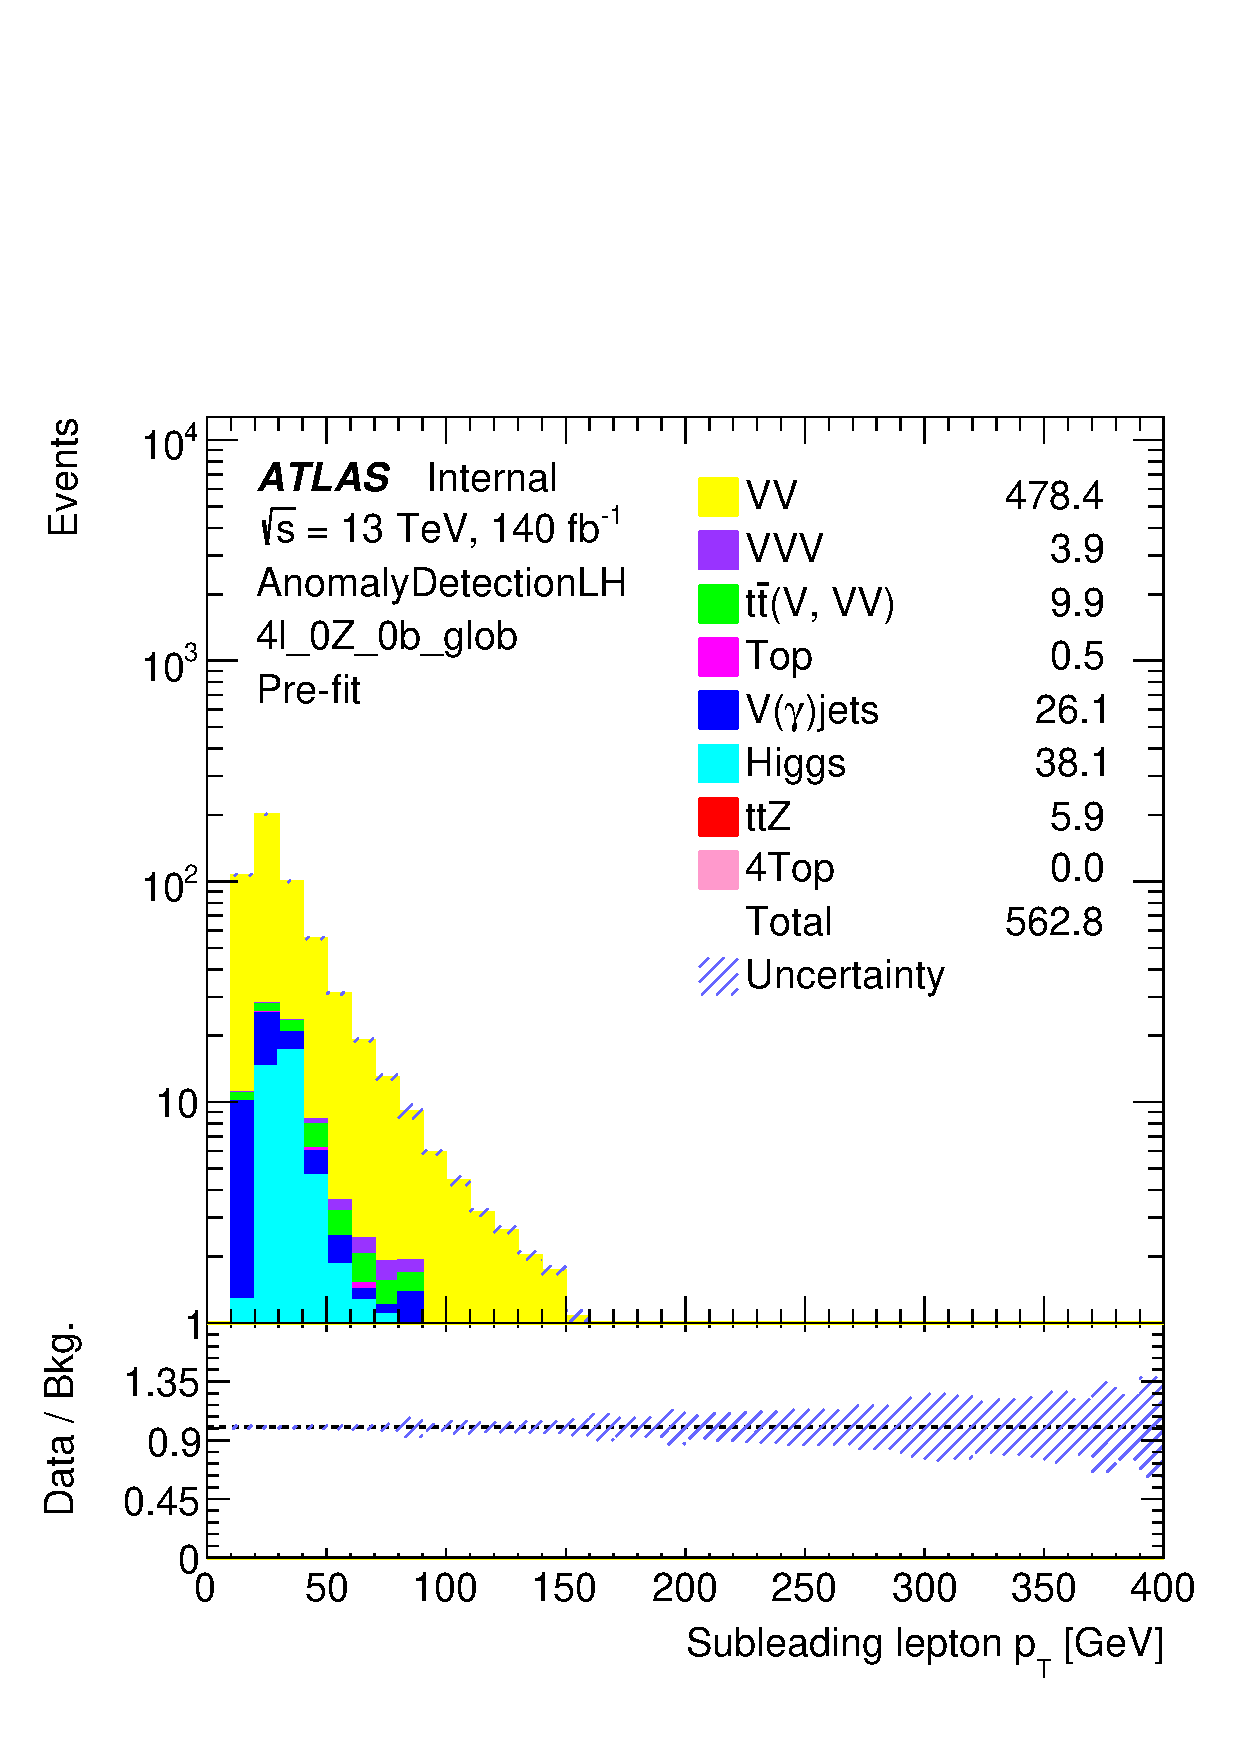
\includegraphics[width=0.24\textwidth]{plots/fourlepLH_run2/Plots/reg_4l_0Z_0b_glob_lep_pt_1.pdf} &
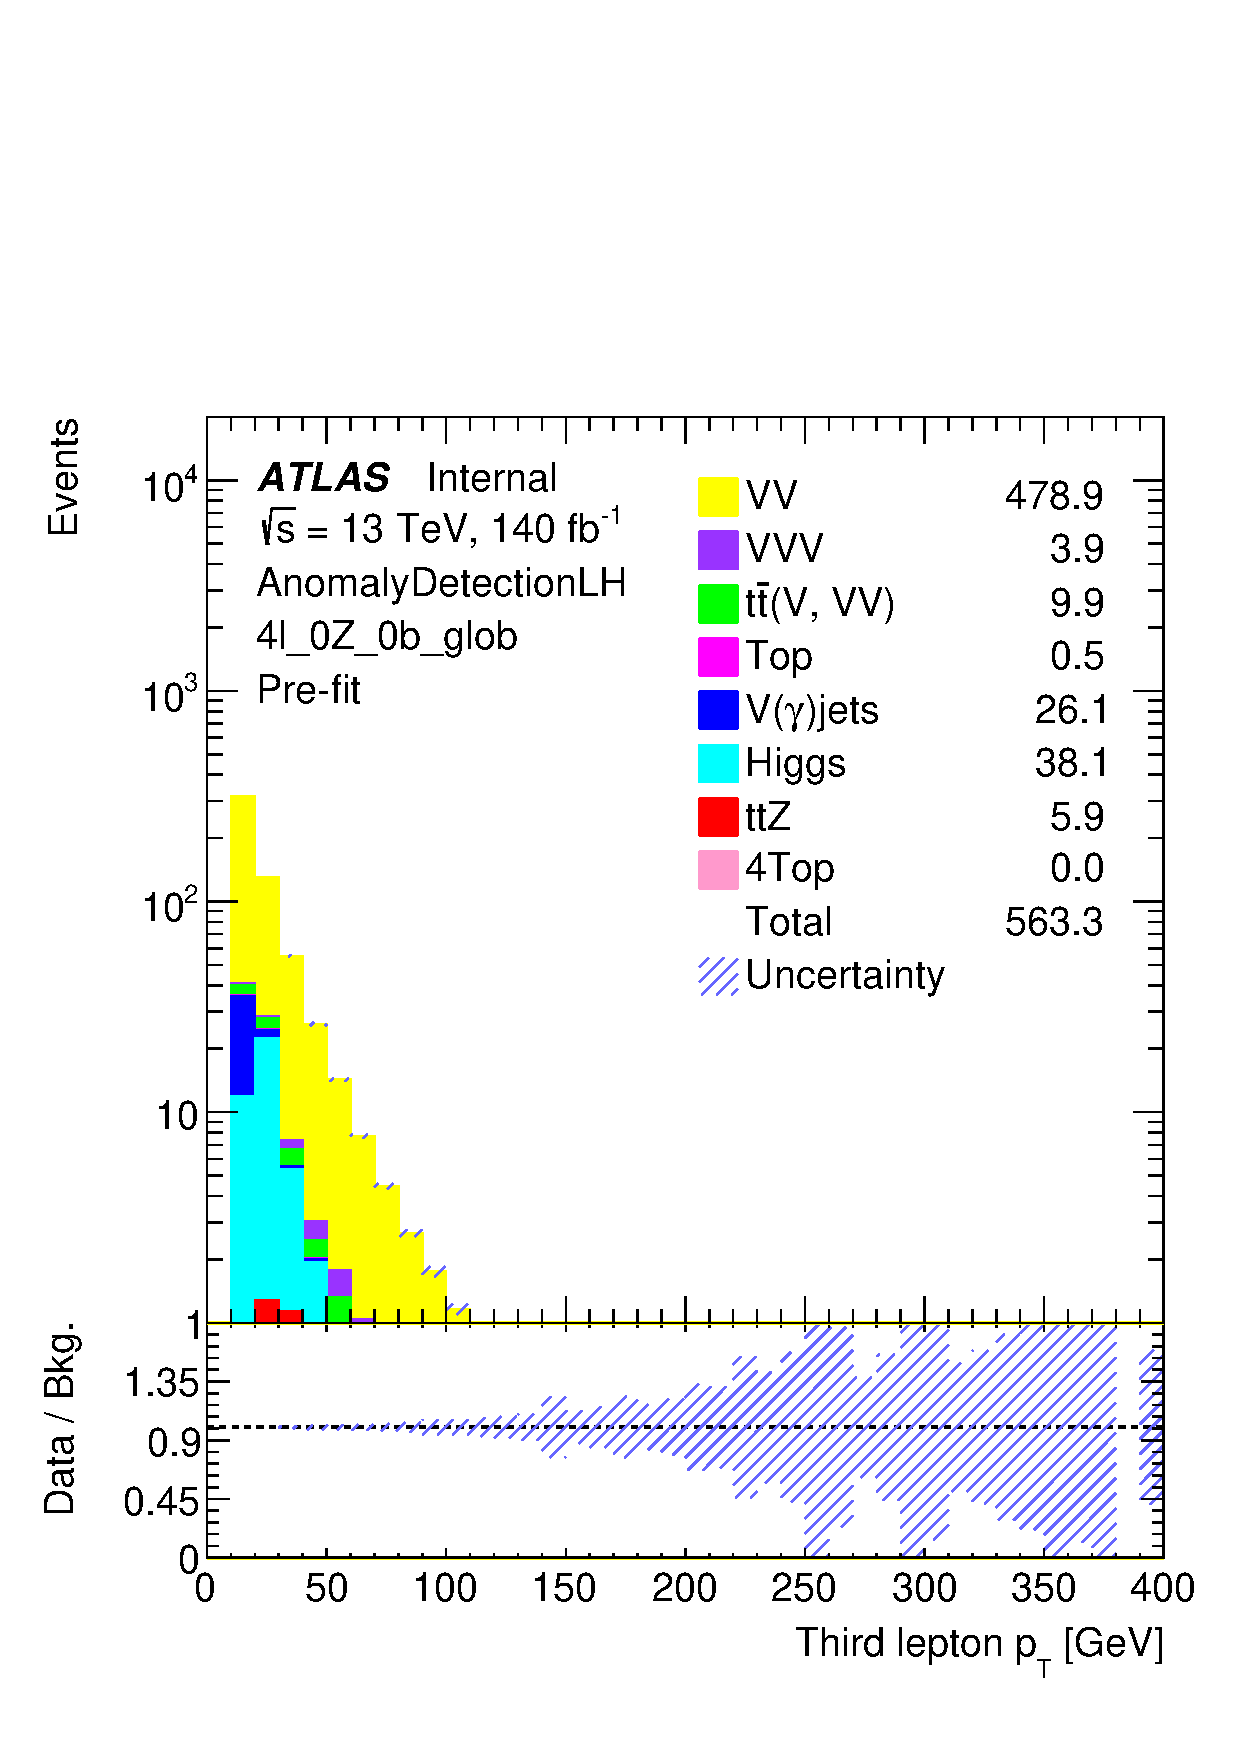
\includegraphics[width=0.24\textwidth]{plots/fourlepLH_run2/Plots/reg_4l_0Z_0b_glob_lep_pt_2.pdf} &
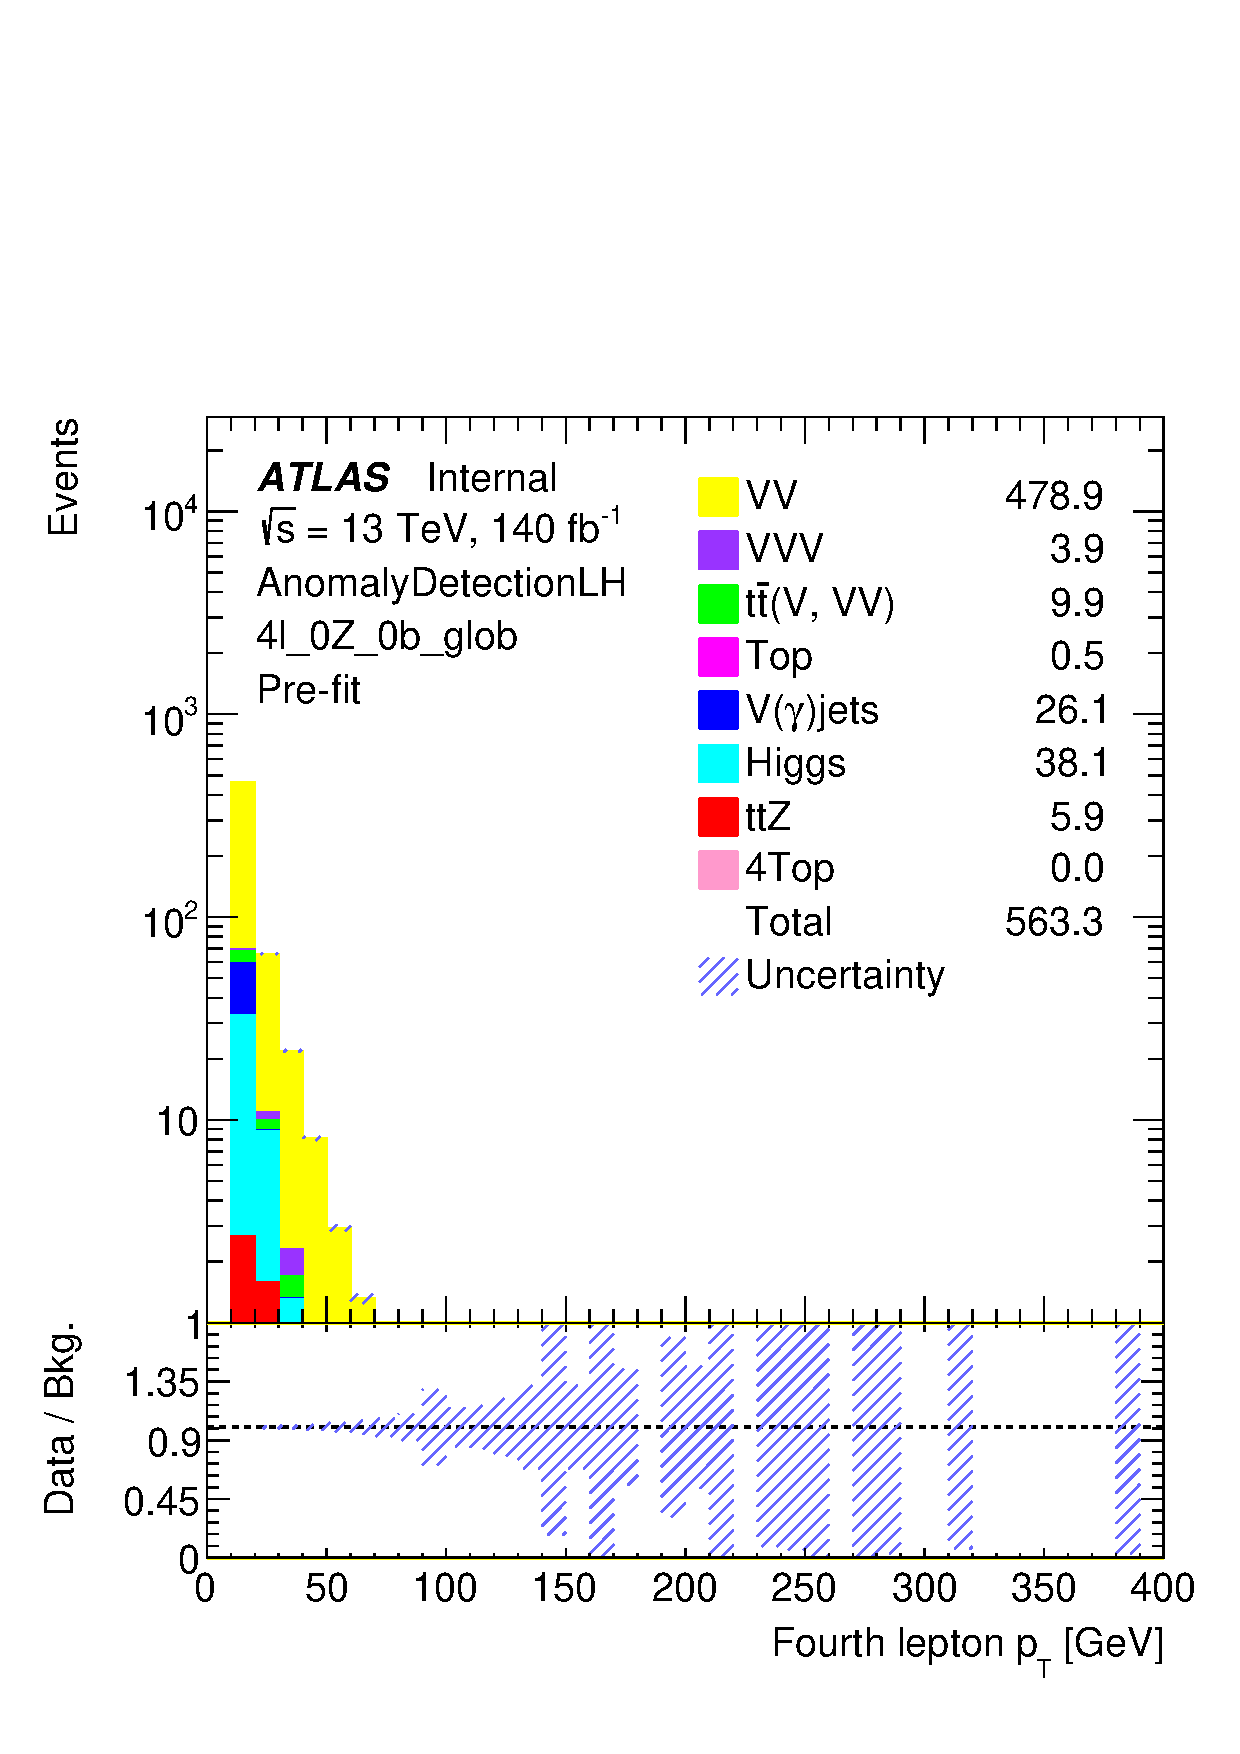
\includegraphics[width=0.24\textwidth]{plots/fourlepLH_run2/Plots/reg_4l_0Z_0b_glob_lep_pt_3.pdf} \\

\end{tabular}

\end{frame}
\subsection{4l\_0Z\_1b}
\begin{frame}{\texttt{Focused selection: 4l\_0Z\_1b}}
%\tiny
\centering
\begin{tabular}{|c|c|}
\hline

4l\_0Z\_1b\_seq &
4l\_0Z\_1b\_glob \\
\hline
\multicolumn{2}{|c|}{\texttt{globalTriggerMatchSLTorDLT\_LooseLH\_custTrig\_NOSYS}} \\
\multicolumn{2}{|c|}{\texttt{pass\_fourlep\_LooseLH\_NOSYS} }\\
\multicolumn{2}{|c|}{\texttt{$N_{leptons}$=4}} \\
\multicolumn{2}{|c|}{\texttt{$N_{taus}$ $\geq 0$} } \\
\multicolumn{2}{|c|}{$N_{b\mathrm{-jets}}$ $\geq 1$} \\
\multicolumn{2}{|c|}{\texttt{Q = 0}} \\

\hline

\texttt{$|m_{Z1}^{seq}-91.2e3| < 10e3$} &
\texttt{$|m_{Z1}^{glob}-91.2e3| < 10e3$} &\\
\texttt{$|m_{Z2}^{seq}-91.2e3| < 10e3$} &
\texttt{$|m_{Z2}^{glob}-91.2e3| < 10e3$}\\

\hline

\end{tabular}
\end{frame}

\begin{frame}{\texttt{Results: 4l\_0Z\_1b}}
\centering
\begin{tabular}{cccccc}

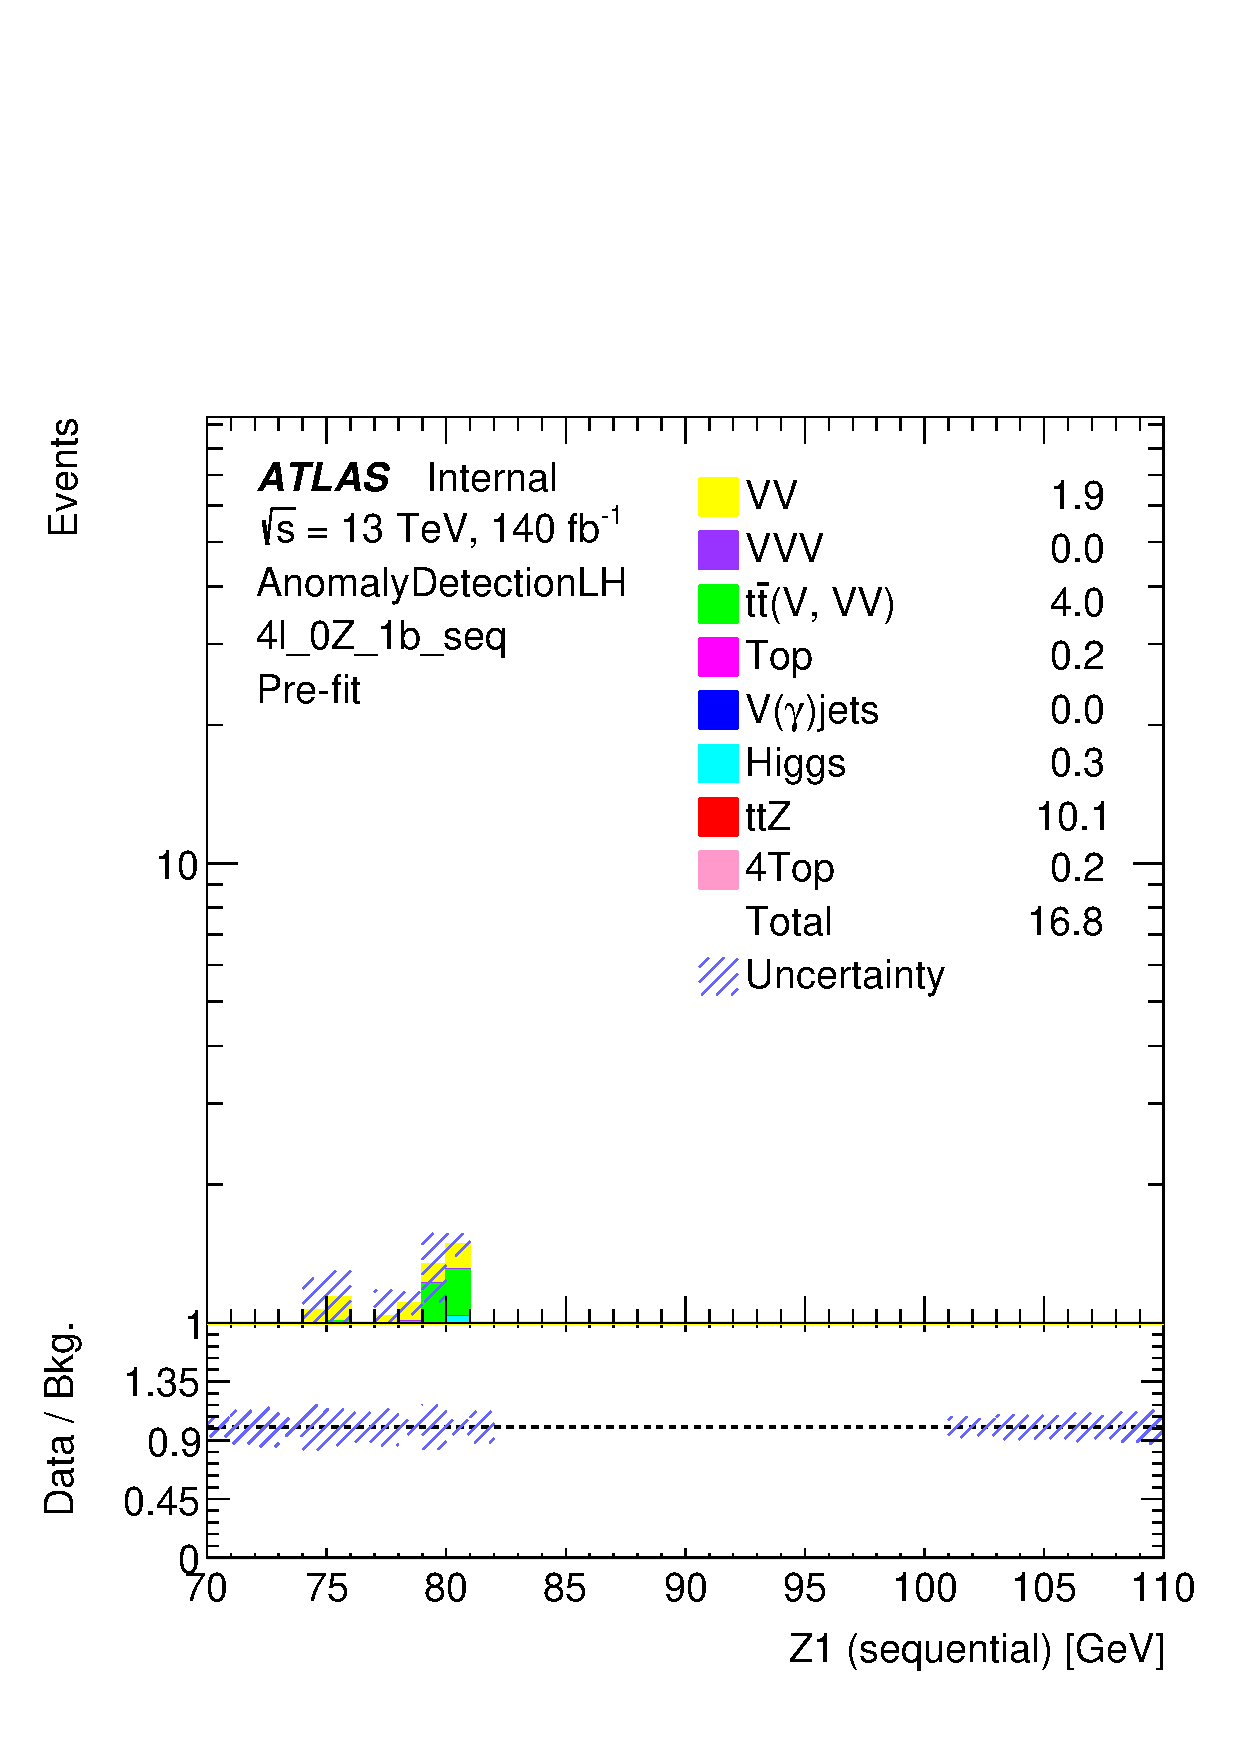
\includegraphics[width=0.24\textwidth]{plots/fourlepLH_run2/Plots/reg_4l_0Z_1b_seq_Z1_mass_seq_1GeV.pdf} &
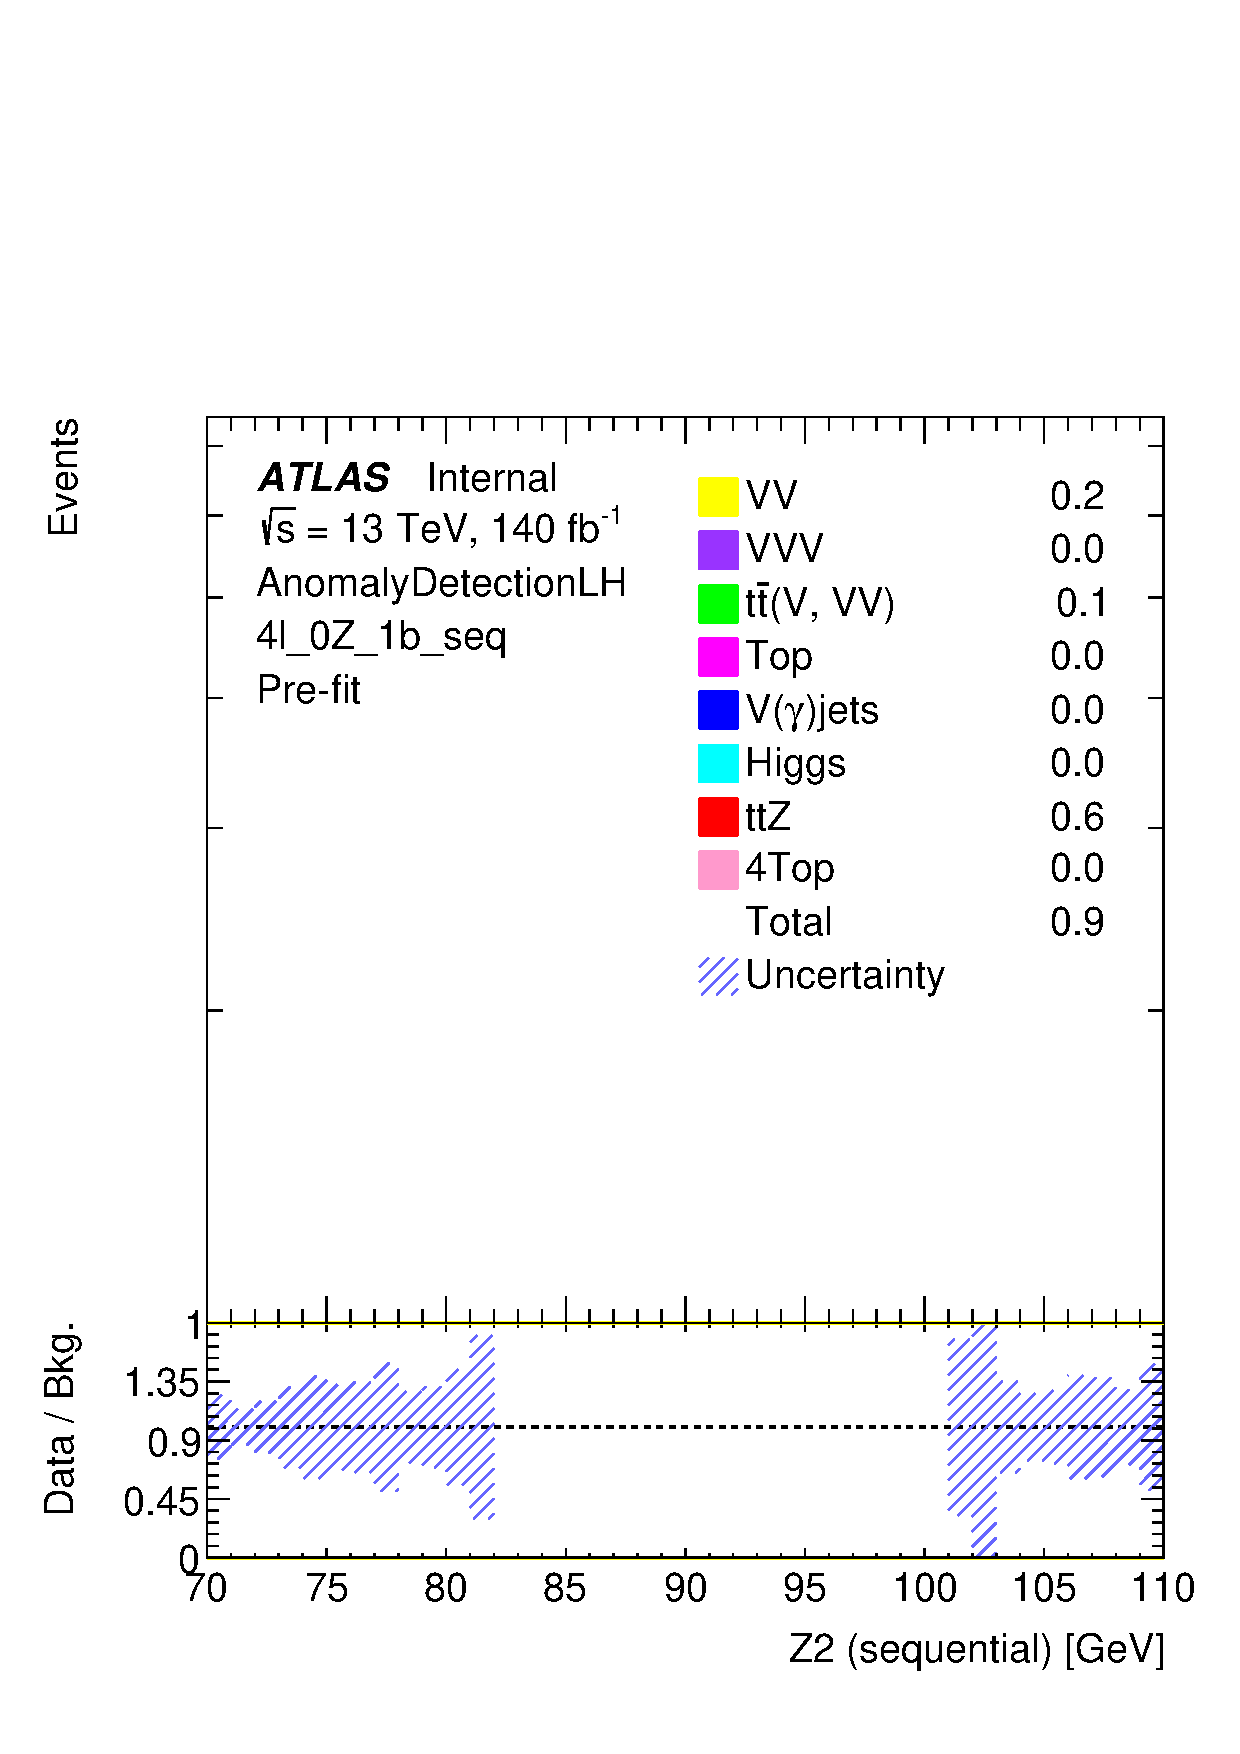
\includegraphics[width=0.24\textwidth]{plots/fourlepLH_run2/Plots/reg_4l_0Z_1b_seq_Z2_mass_seq_1GeV.pdf}  &

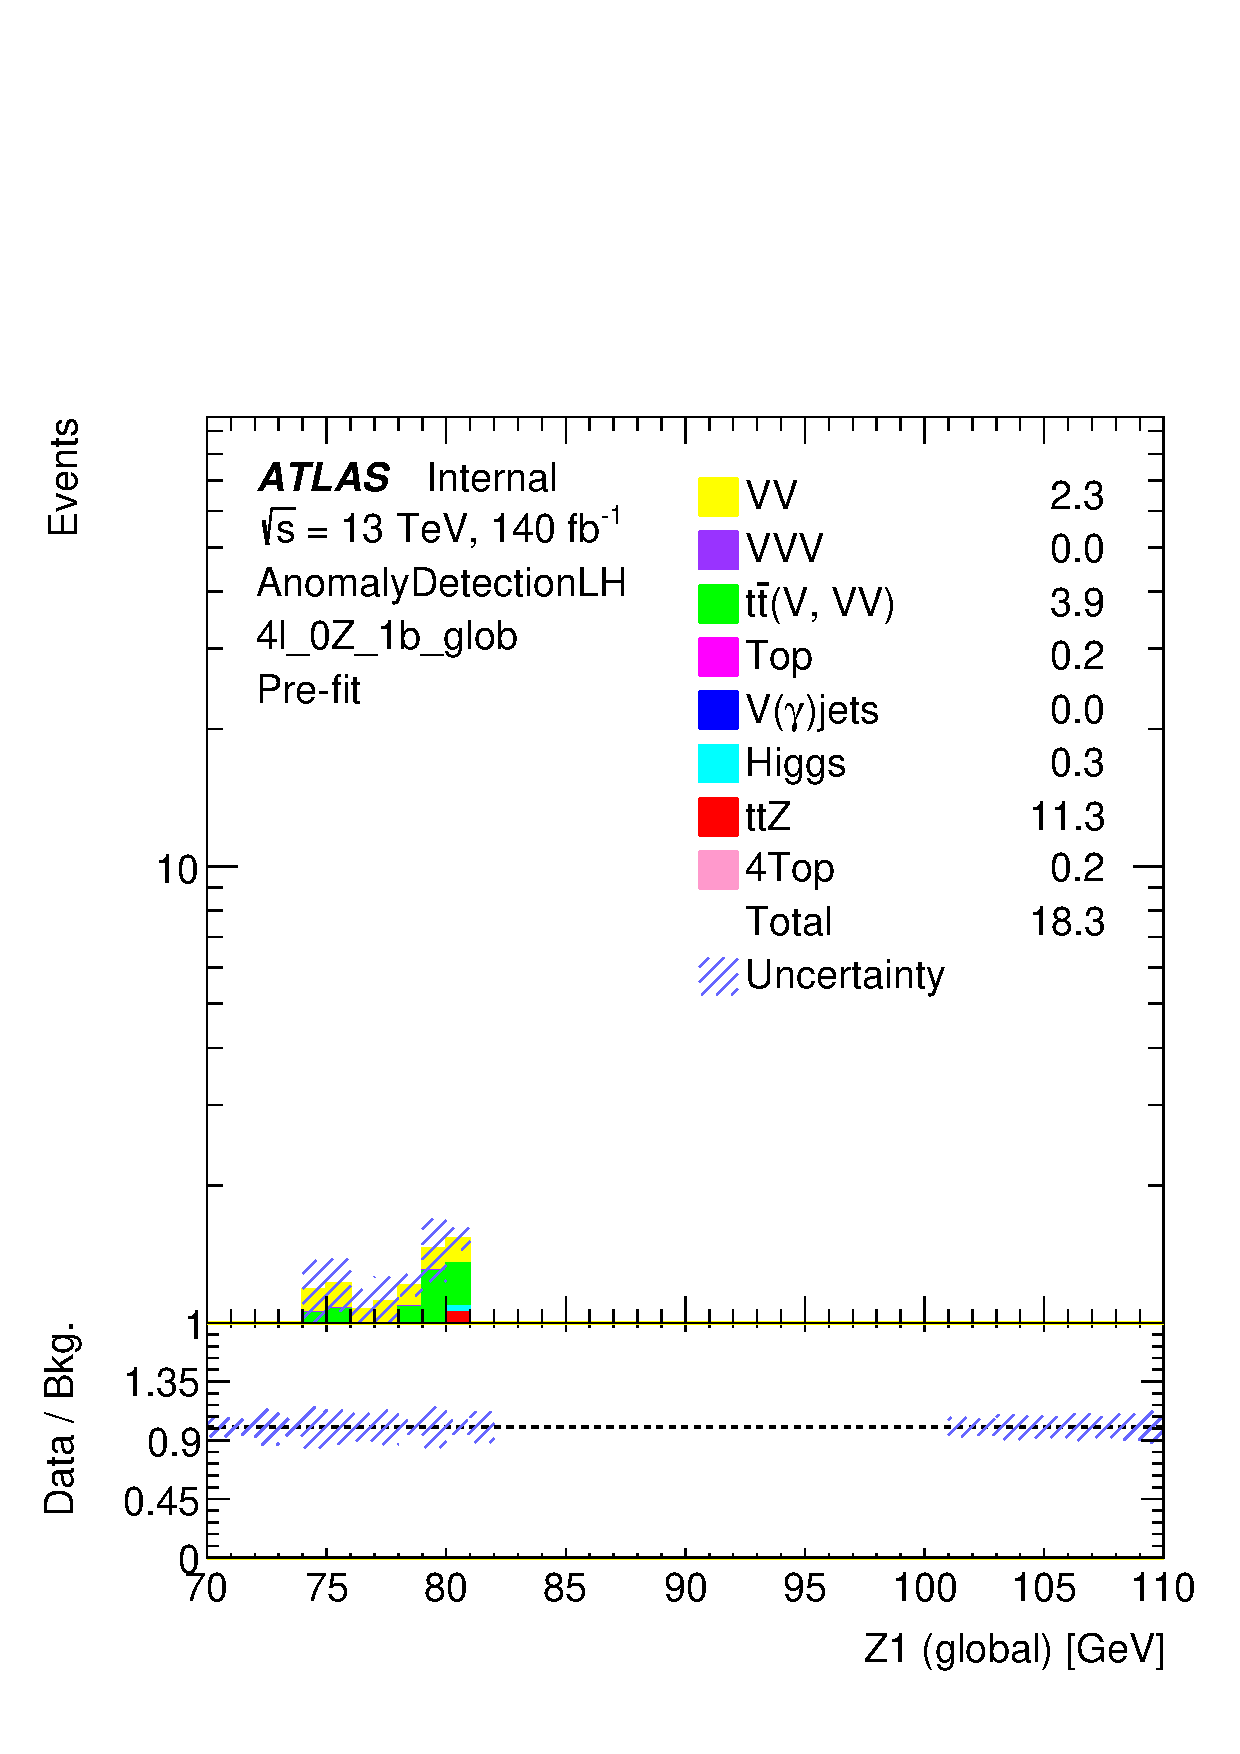
\includegraphics[width=0.24\textwidth]{plots/fourlepLH_run2/Plots/reg_4l_0Z_1b_glob_Z1_mass_glob_1GeV.pdf} &
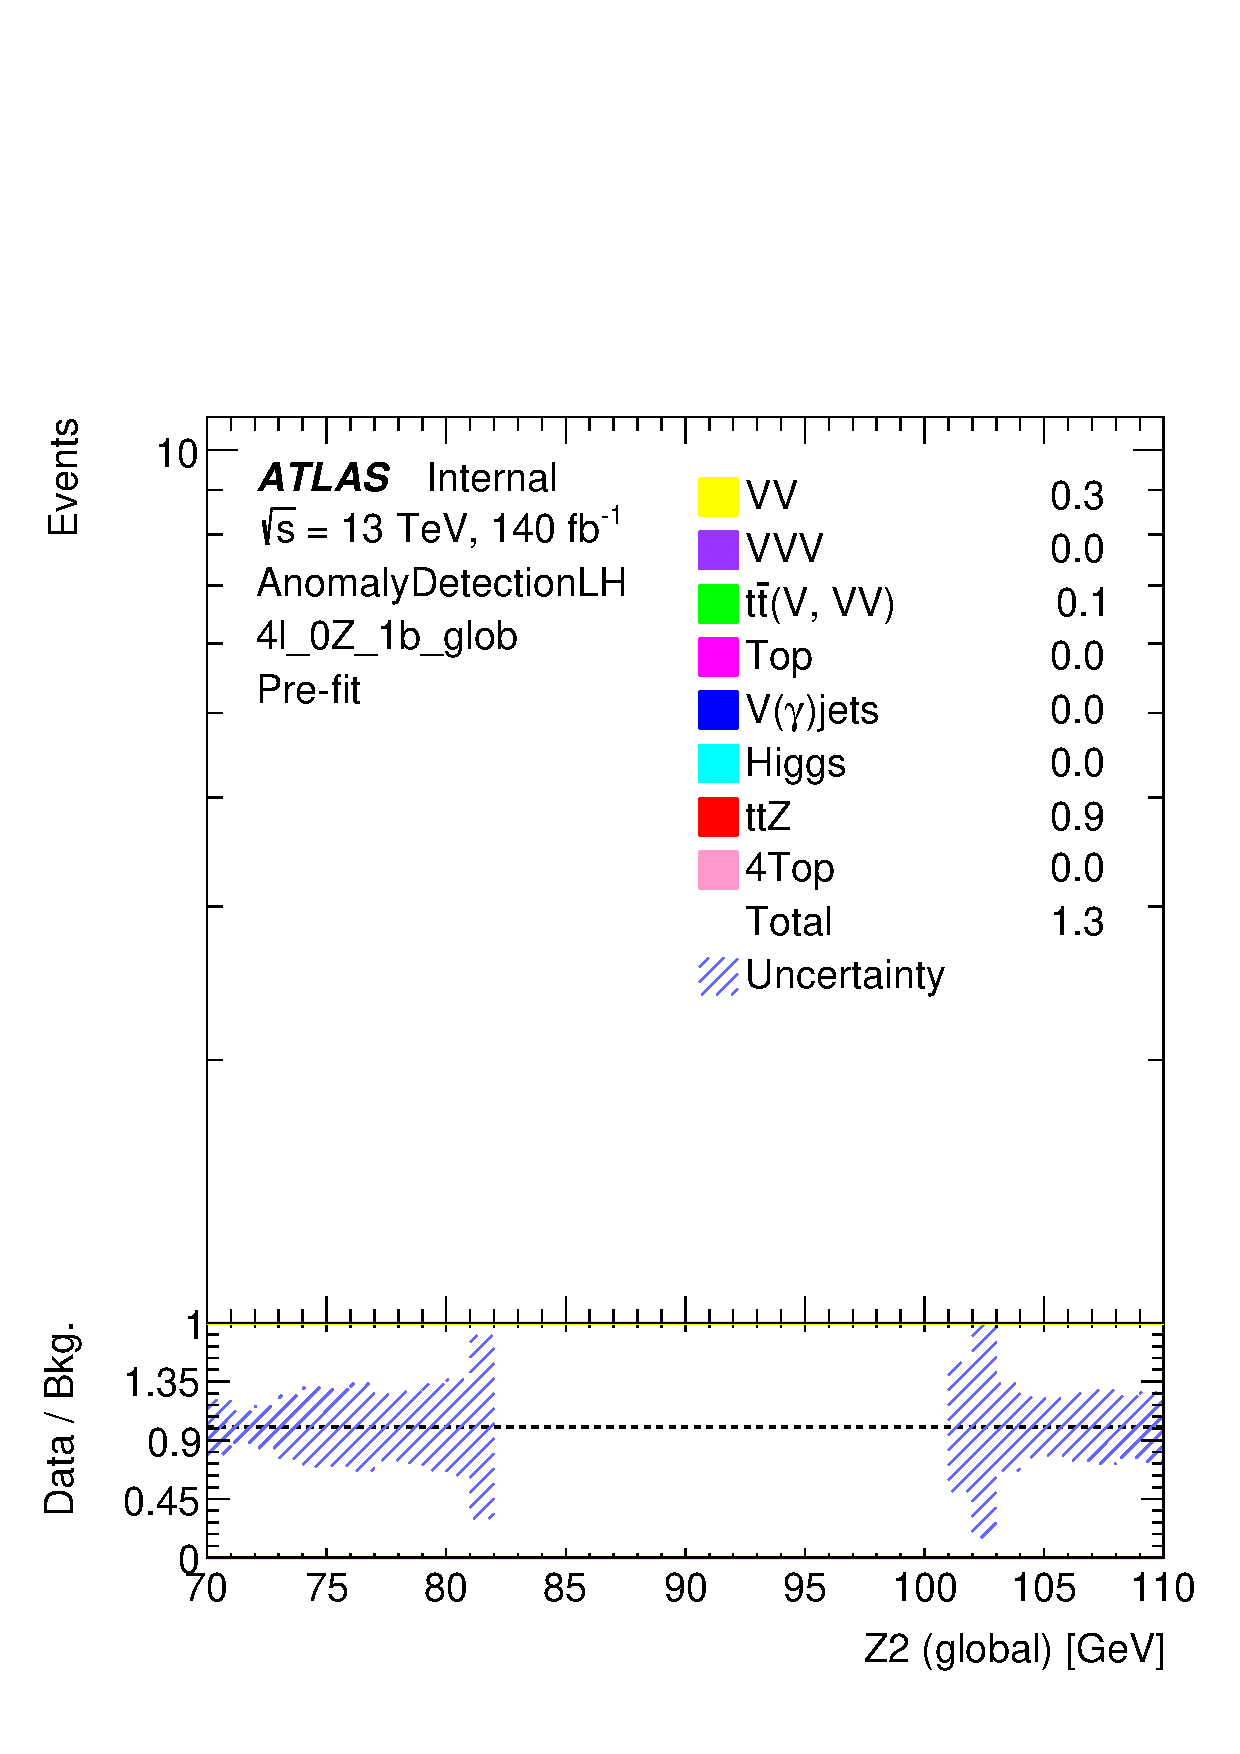
\includegraphics[width=0.24\textwidth]{plots/fourlepLH_run2/Plots/reg_4l_0Z_1b_glob_Z2_mass_glob_1GeV.pdf}\\

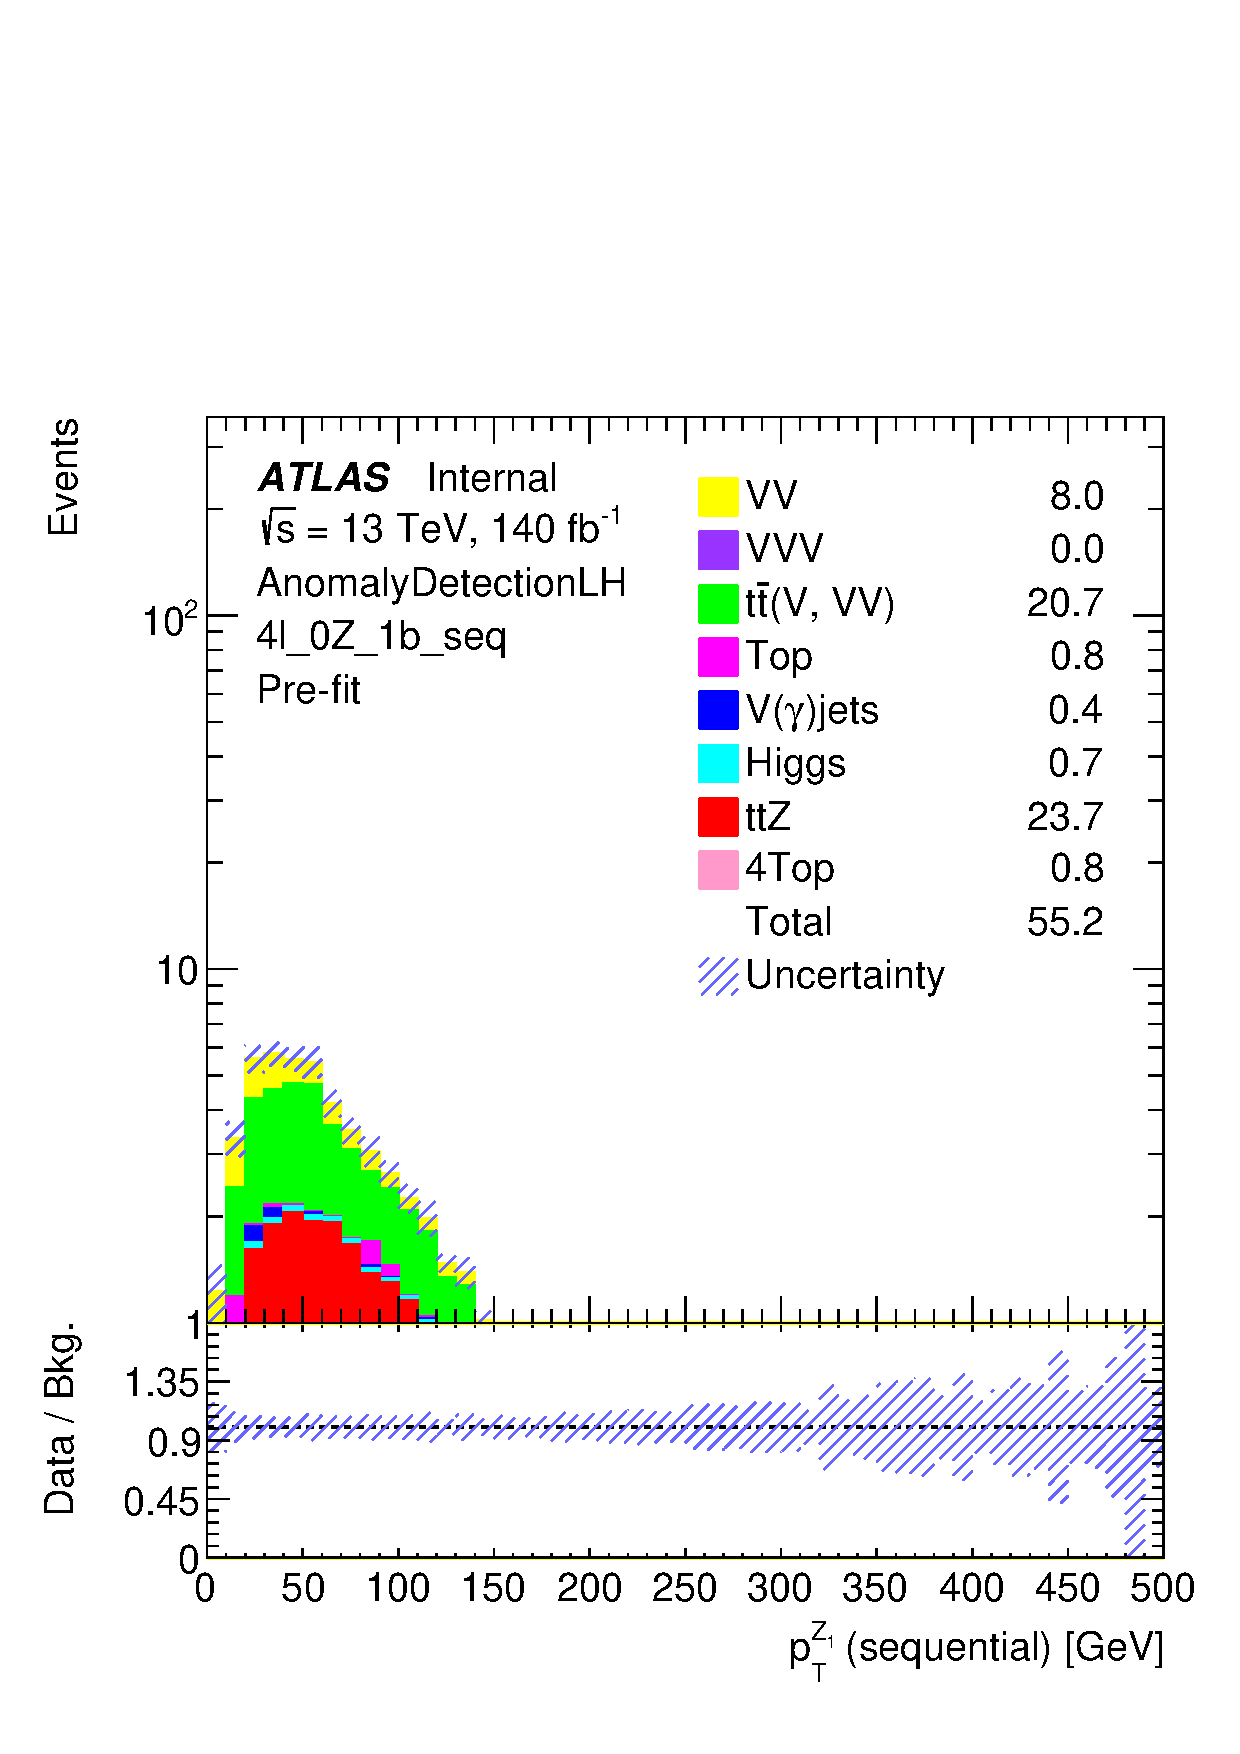
\includegraphics[width=0.24\textwidth]{plots/fourlepLH_run2/Plots/reg_4l_0Z_1b_seq_Z1_pt_seq.pdf} &
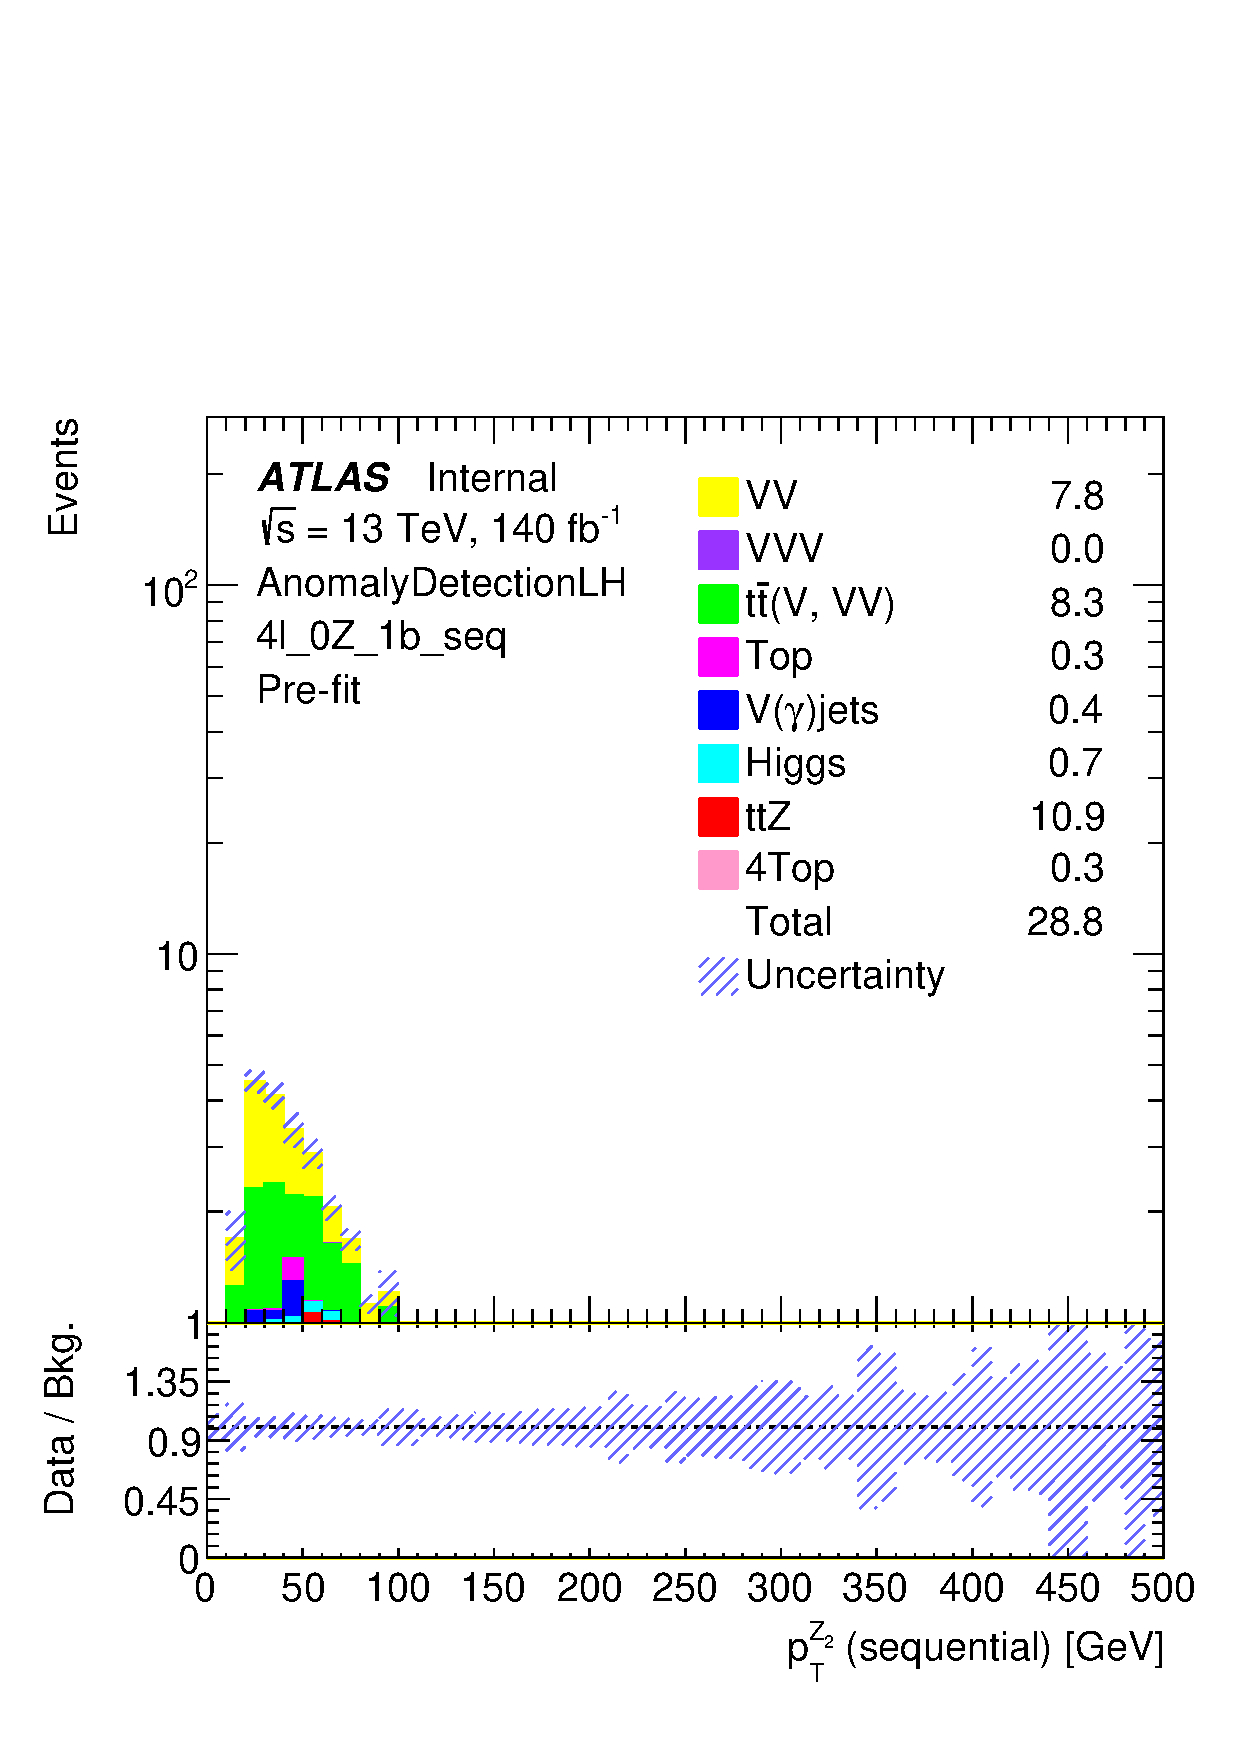
\includegraphics[width=0.24\textwidth]{plots/fourlepLH_run2/Plots/reg_4l_0Z_1b_seq_Z2_pt_seq.pdf}  &

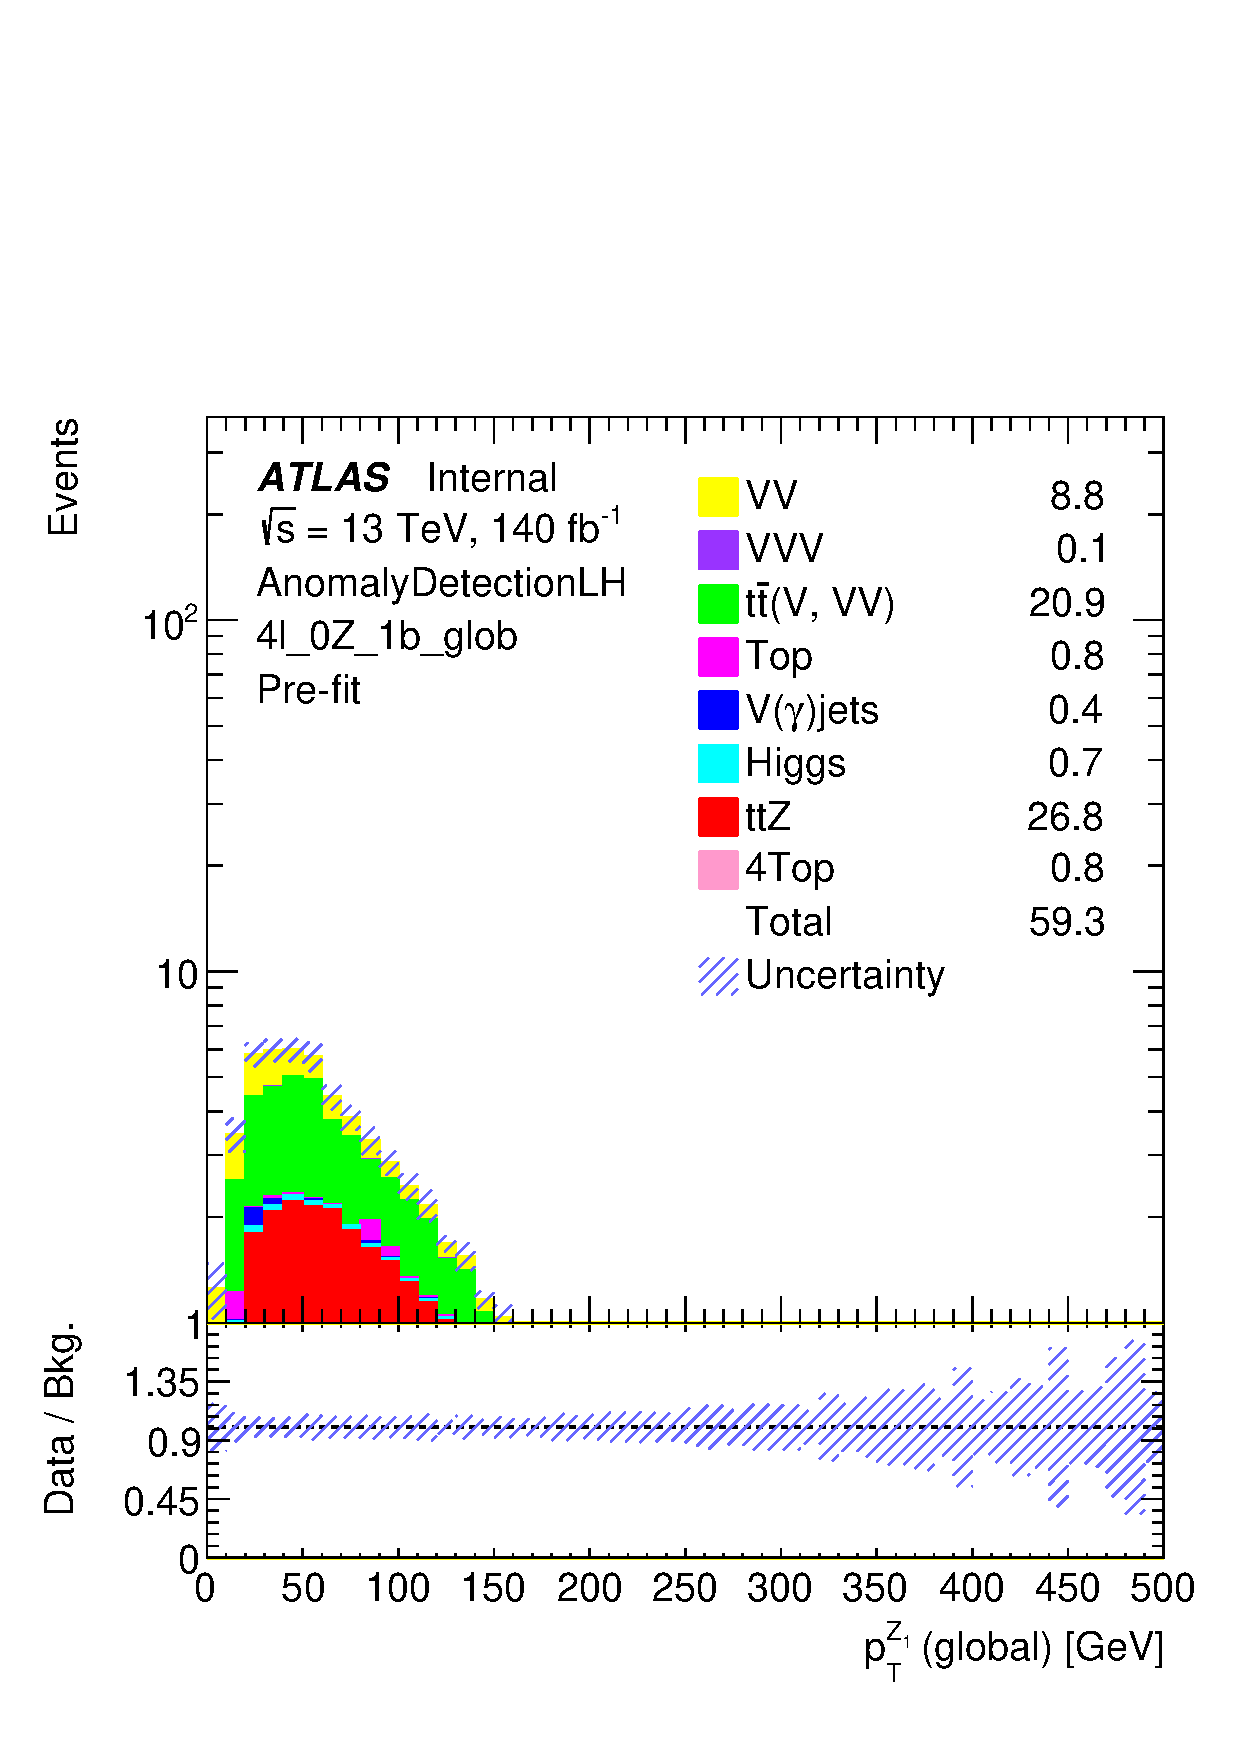
\includegraphics[width=0.24\textwidth]{plots/fourlepLH_run2/Plots/reg_4l_0Z_1b_glob_Z1_pt_glob.pdf} &
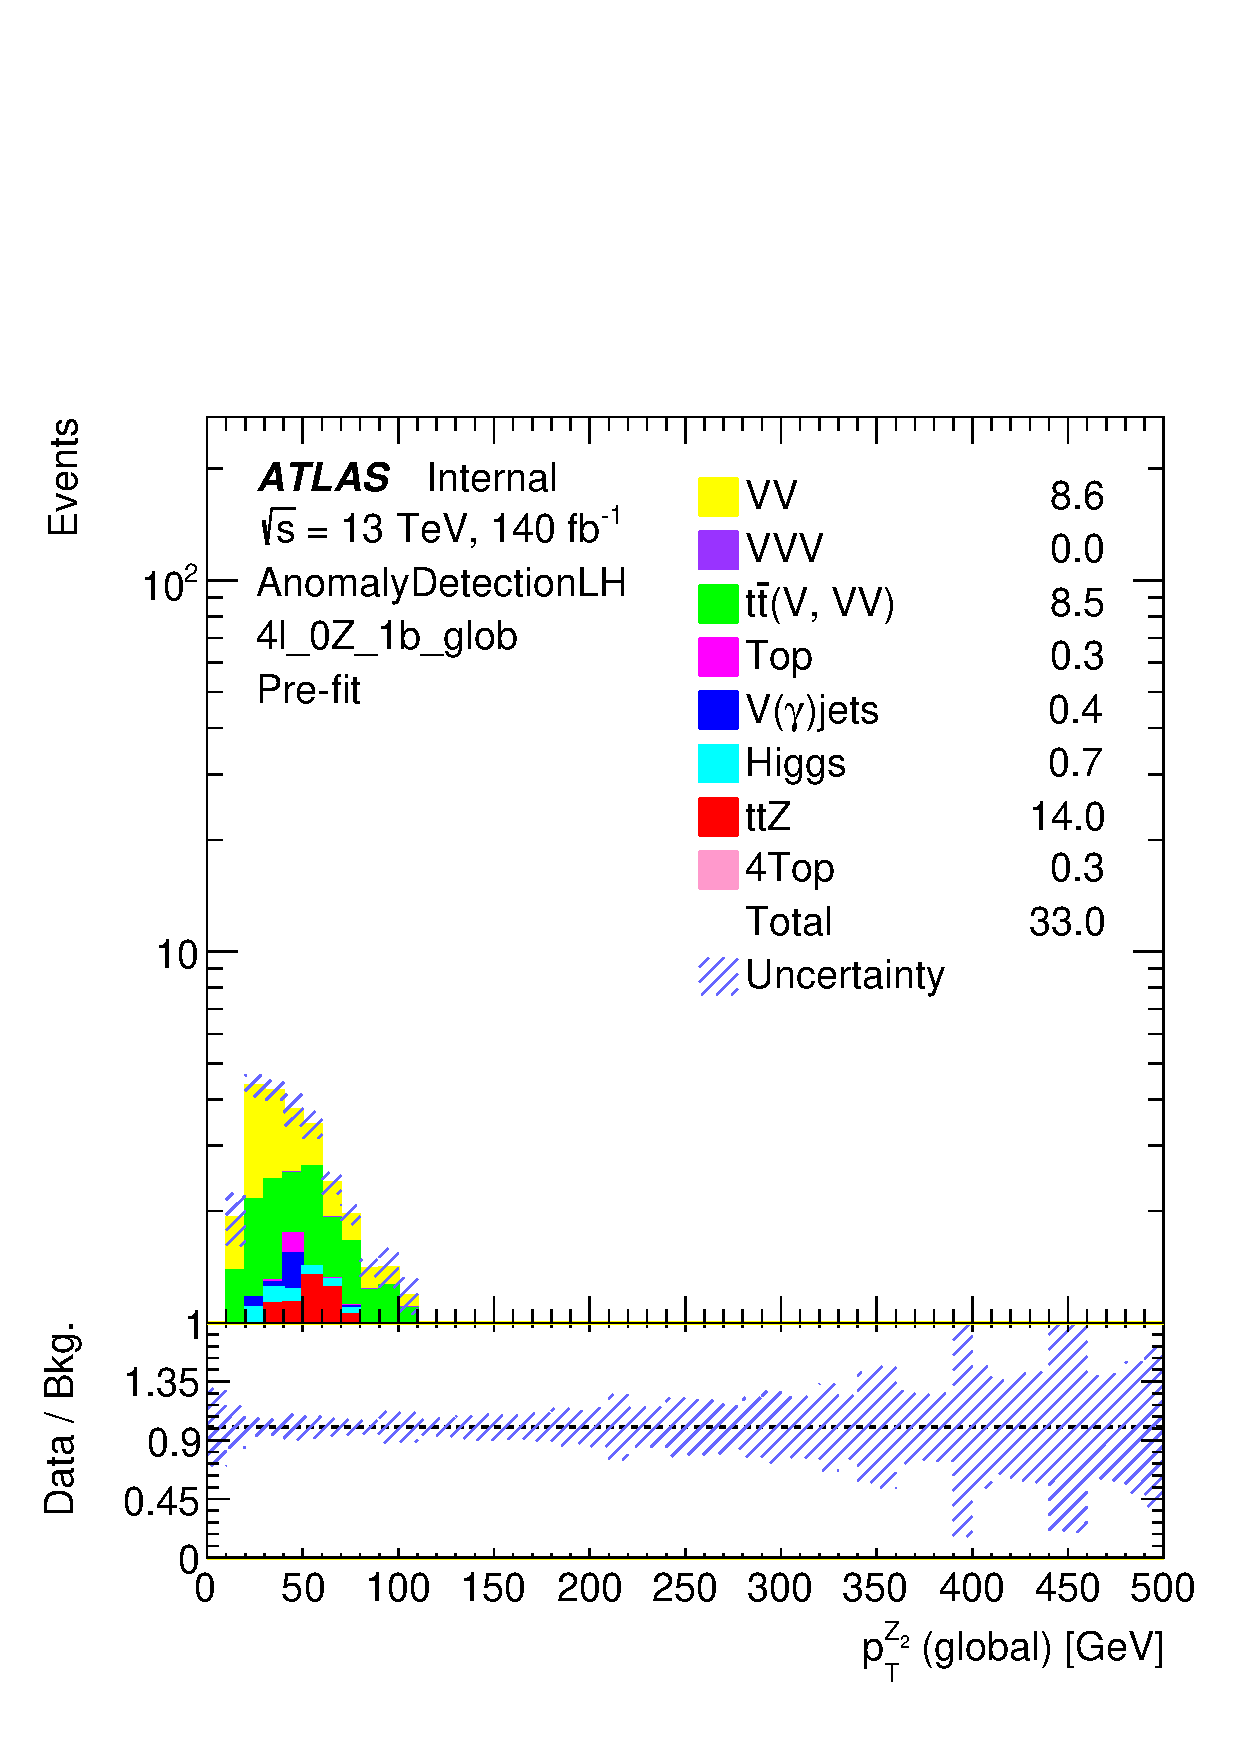
\includegraphics[width=0.24\textwidth]{plots/fourlepLH_run2/Plots/reg_4l_0Z_1b_glob_Z2_pt_glob.pdf}
\end{tabular}
\end{frame}

\begin{frame}{\texttt{Results: 4l\_0Z\_1b}}
\begin{tabular}{cccccc}
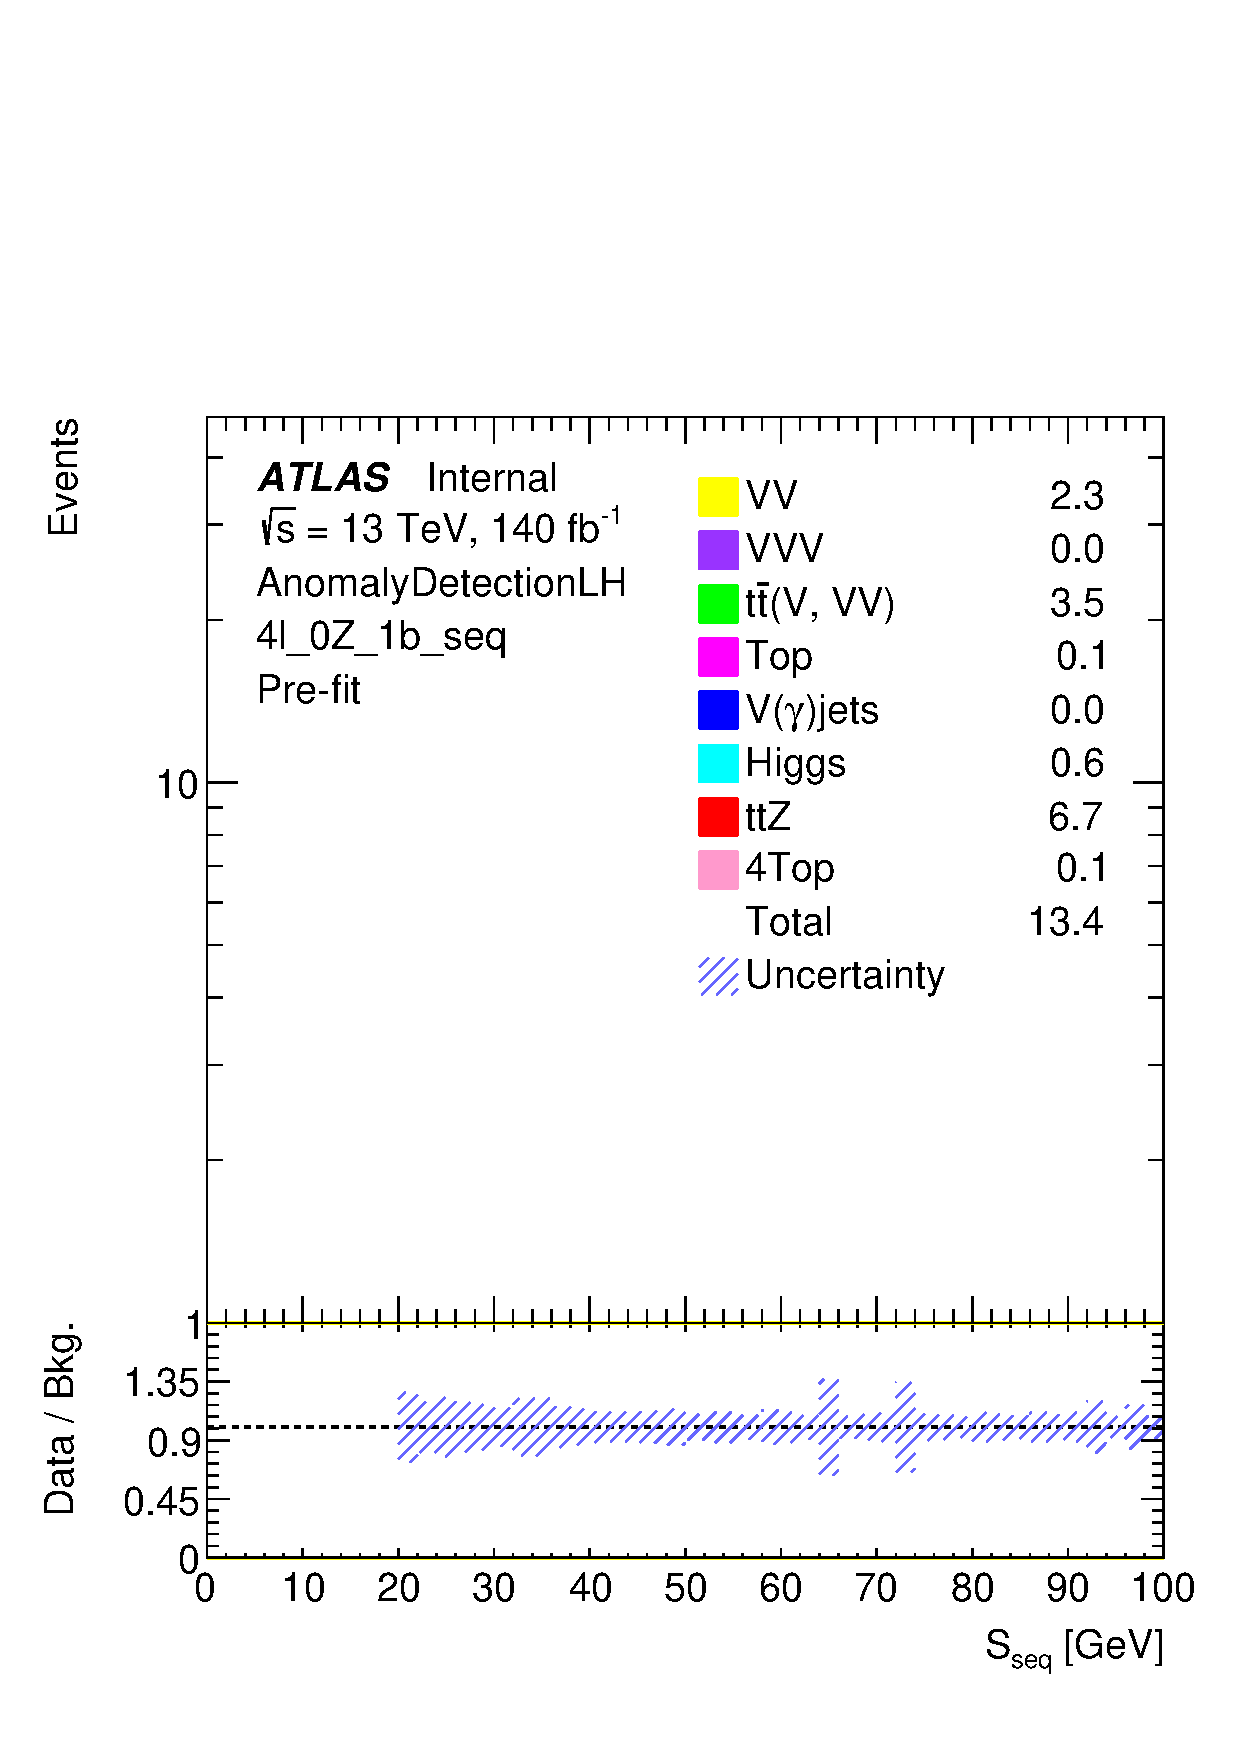
\includegraphics[width=0.24\textwidth]{plots/fourlepLH_run2/Plots/reg_4l_0Z_1b_seq_Zscore_seq.pdf} & 
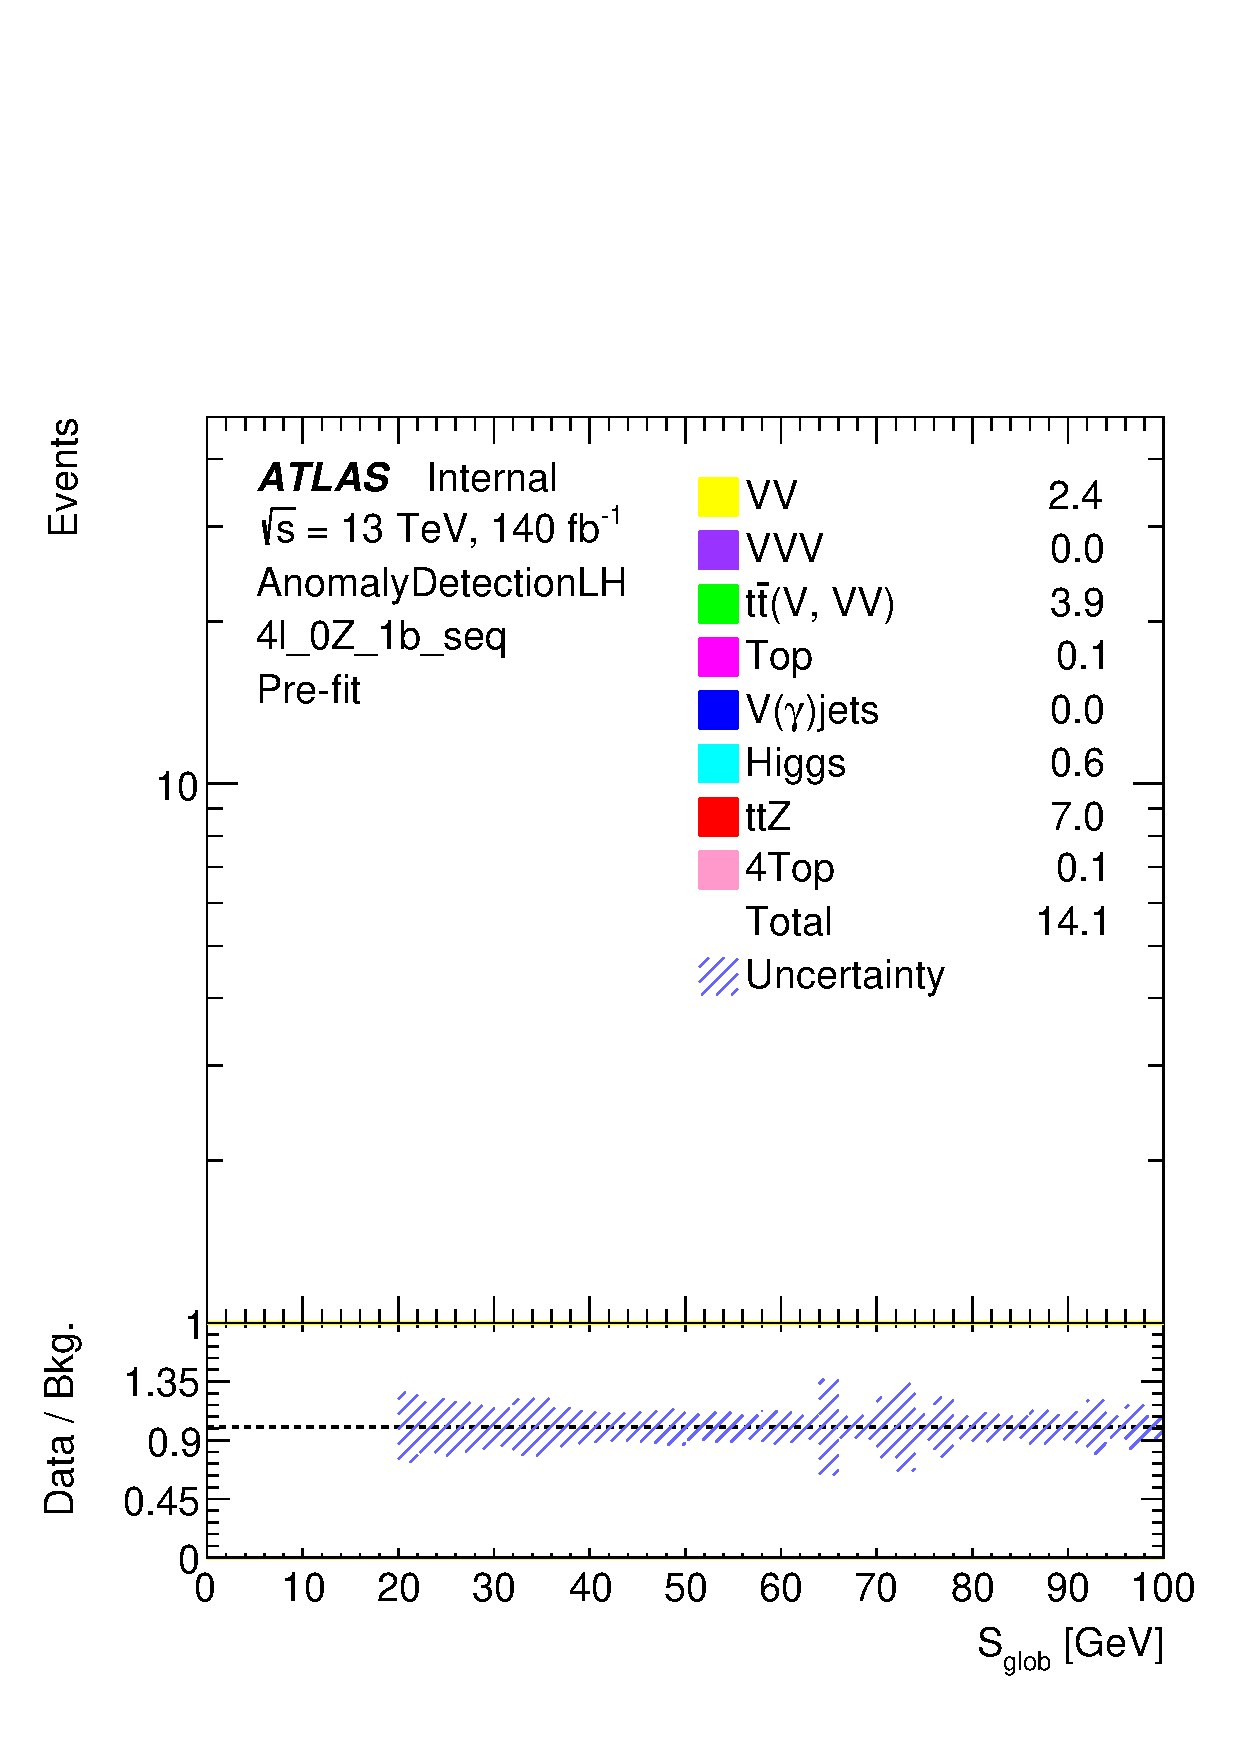
\includegraphics[width=0.24\textwidth]{plots/fourlepLH_run2/Plots/reg_4l_0Z_1b_seq_Zscore_glob.pdf}&
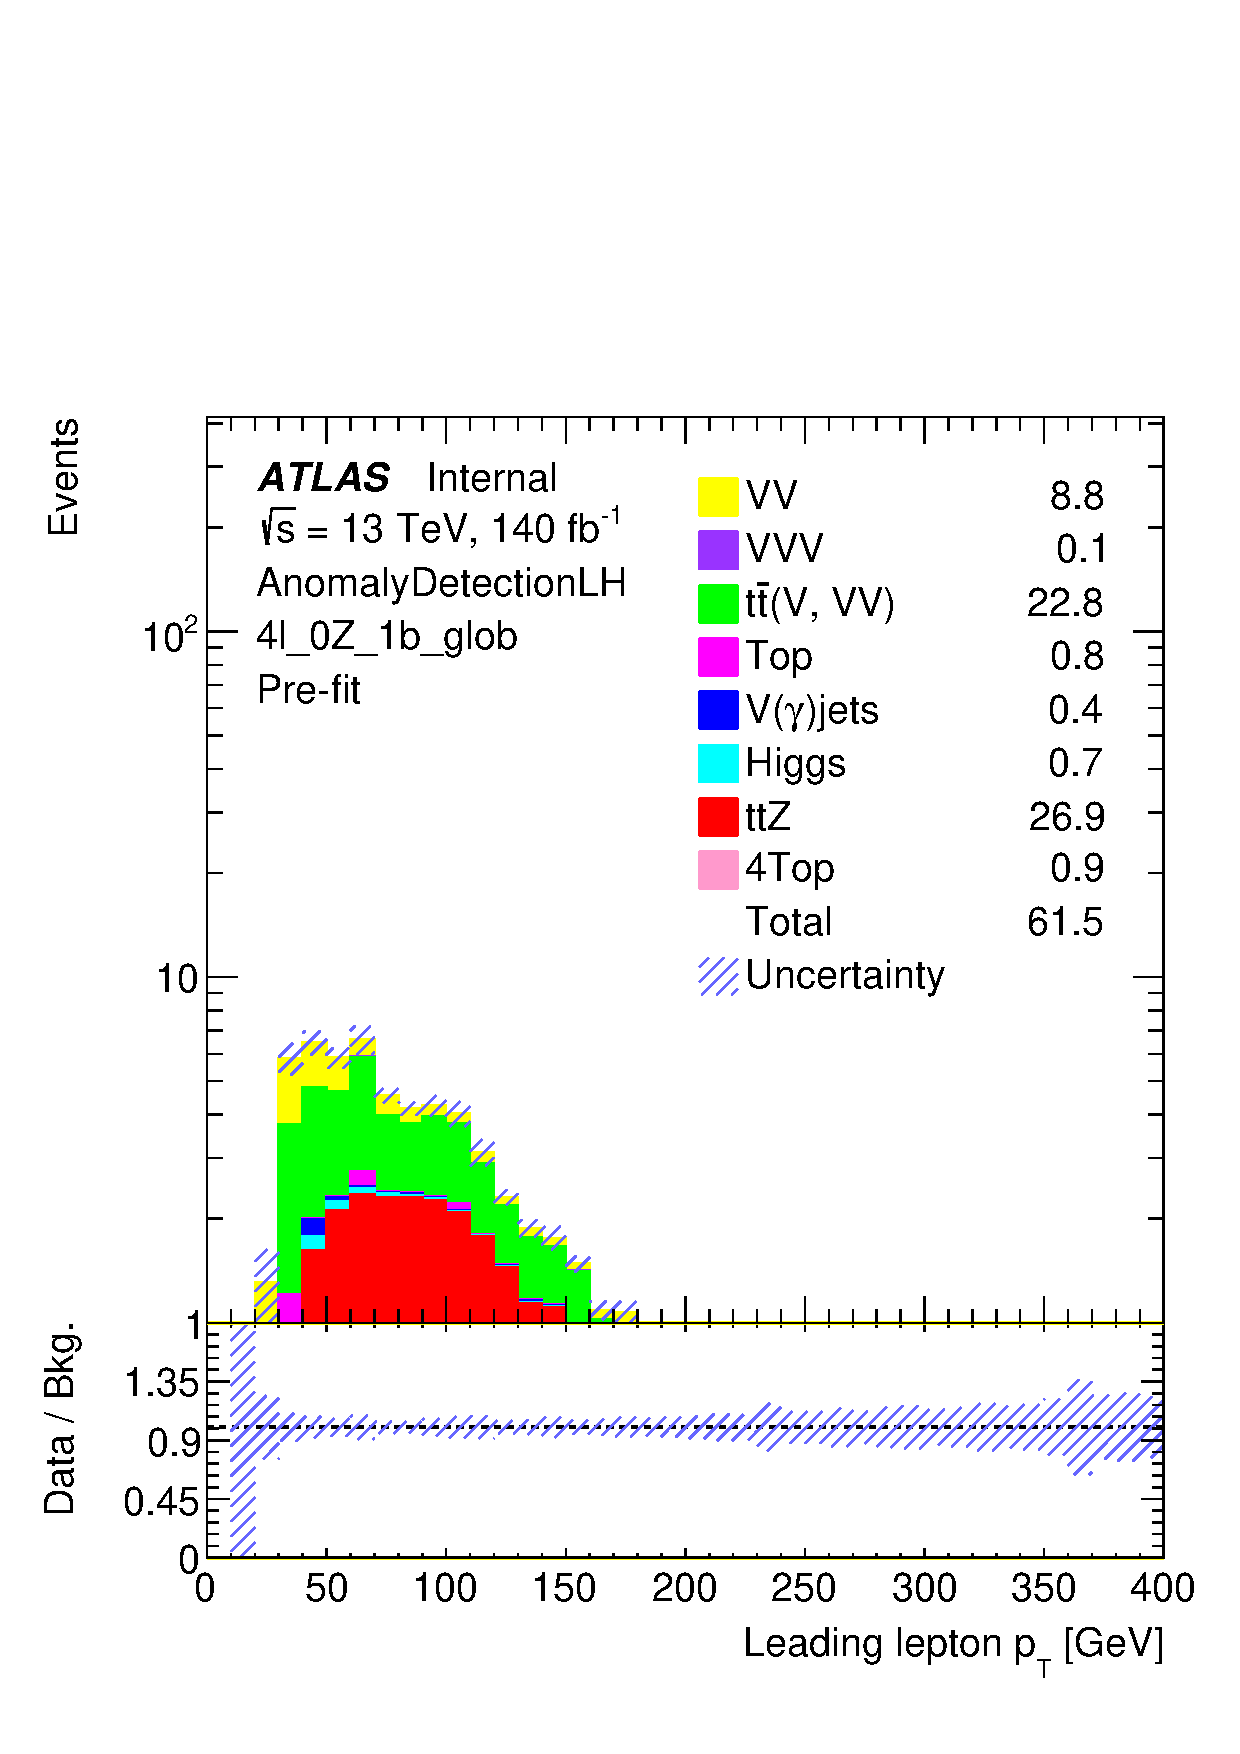
\includegraphics[width=0.24\textwidth]{plots/fourlepLH_run2/Plots/reg_4l_0Z_1b_seq_deltaZscore.pdf}\\

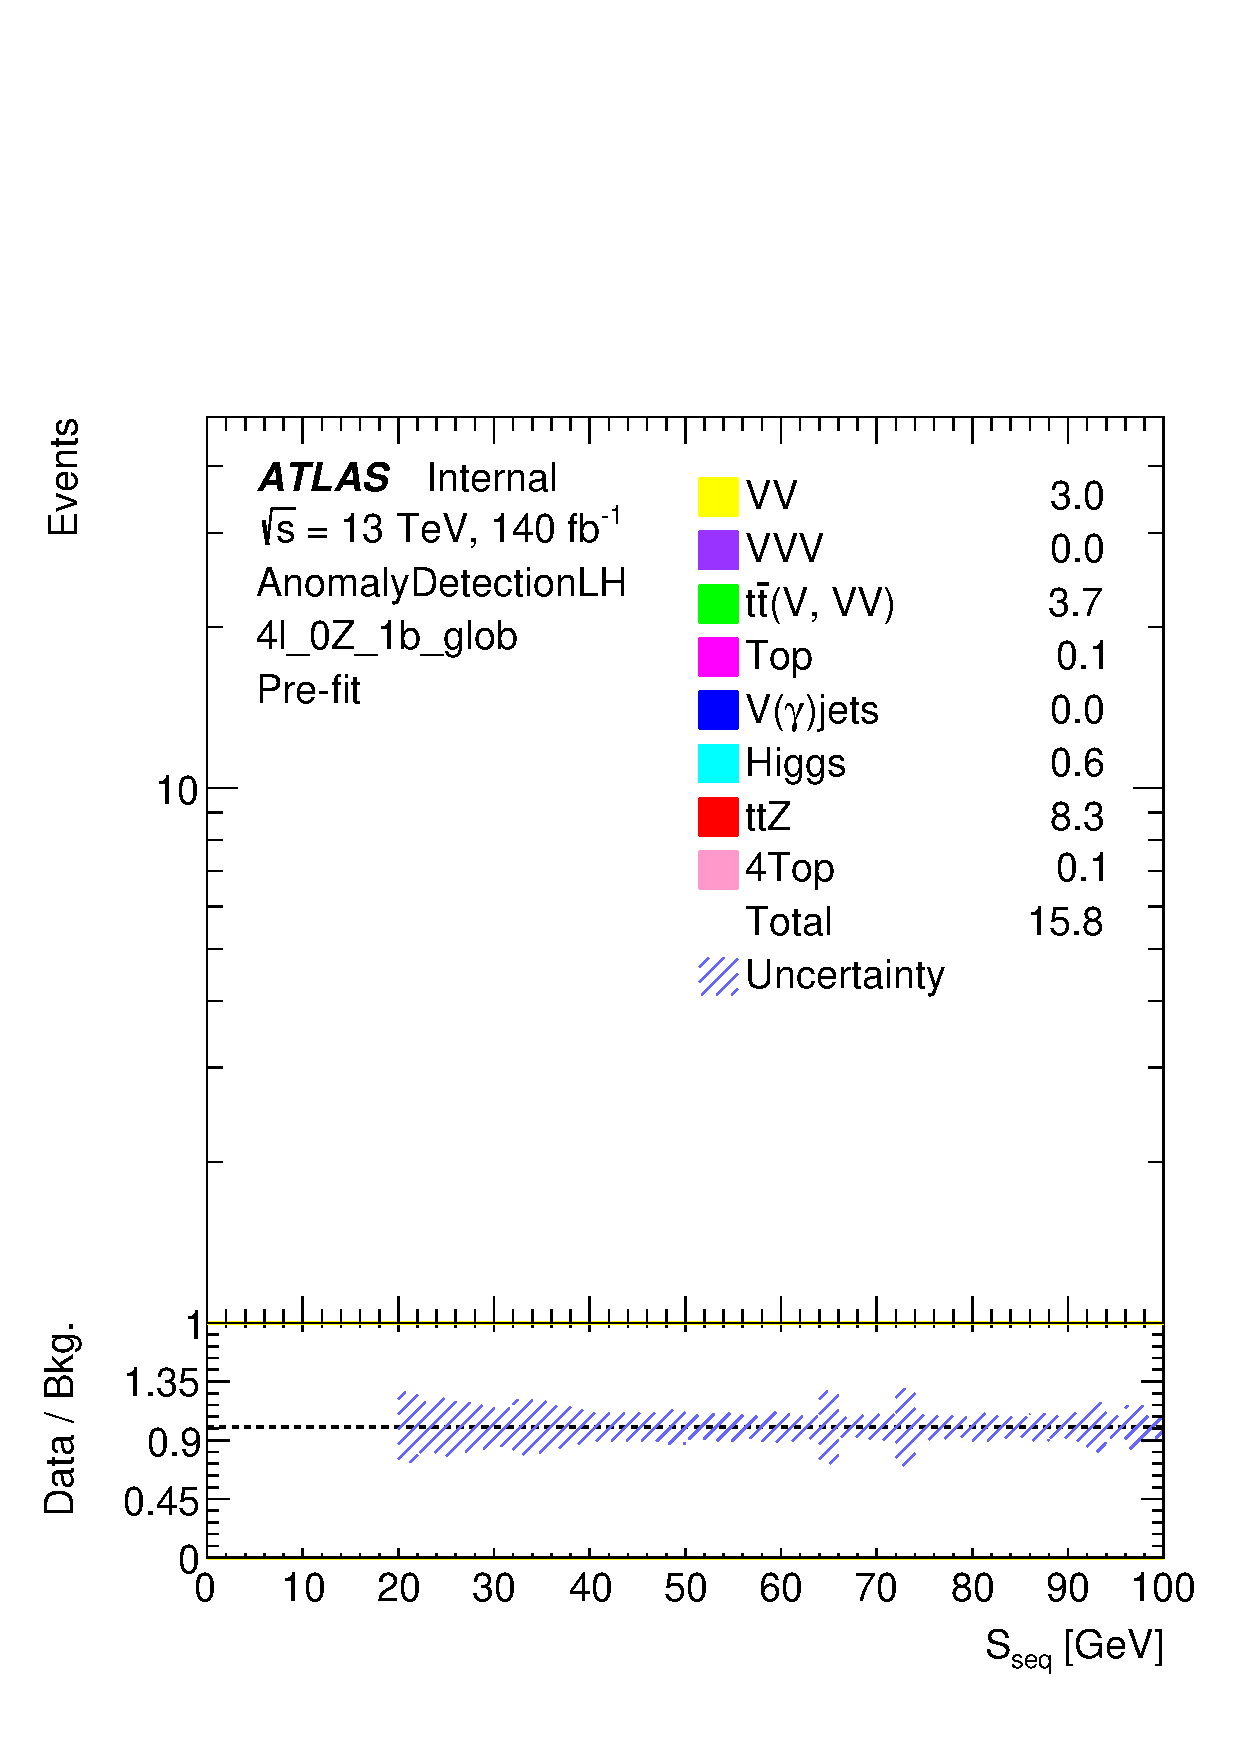
\includegraphics[width=0.24\textwidth]{plots/fourlepLH_run2/Plots/reg_4l_0Z_1b_glob_Zscore_seq.pdf} & 
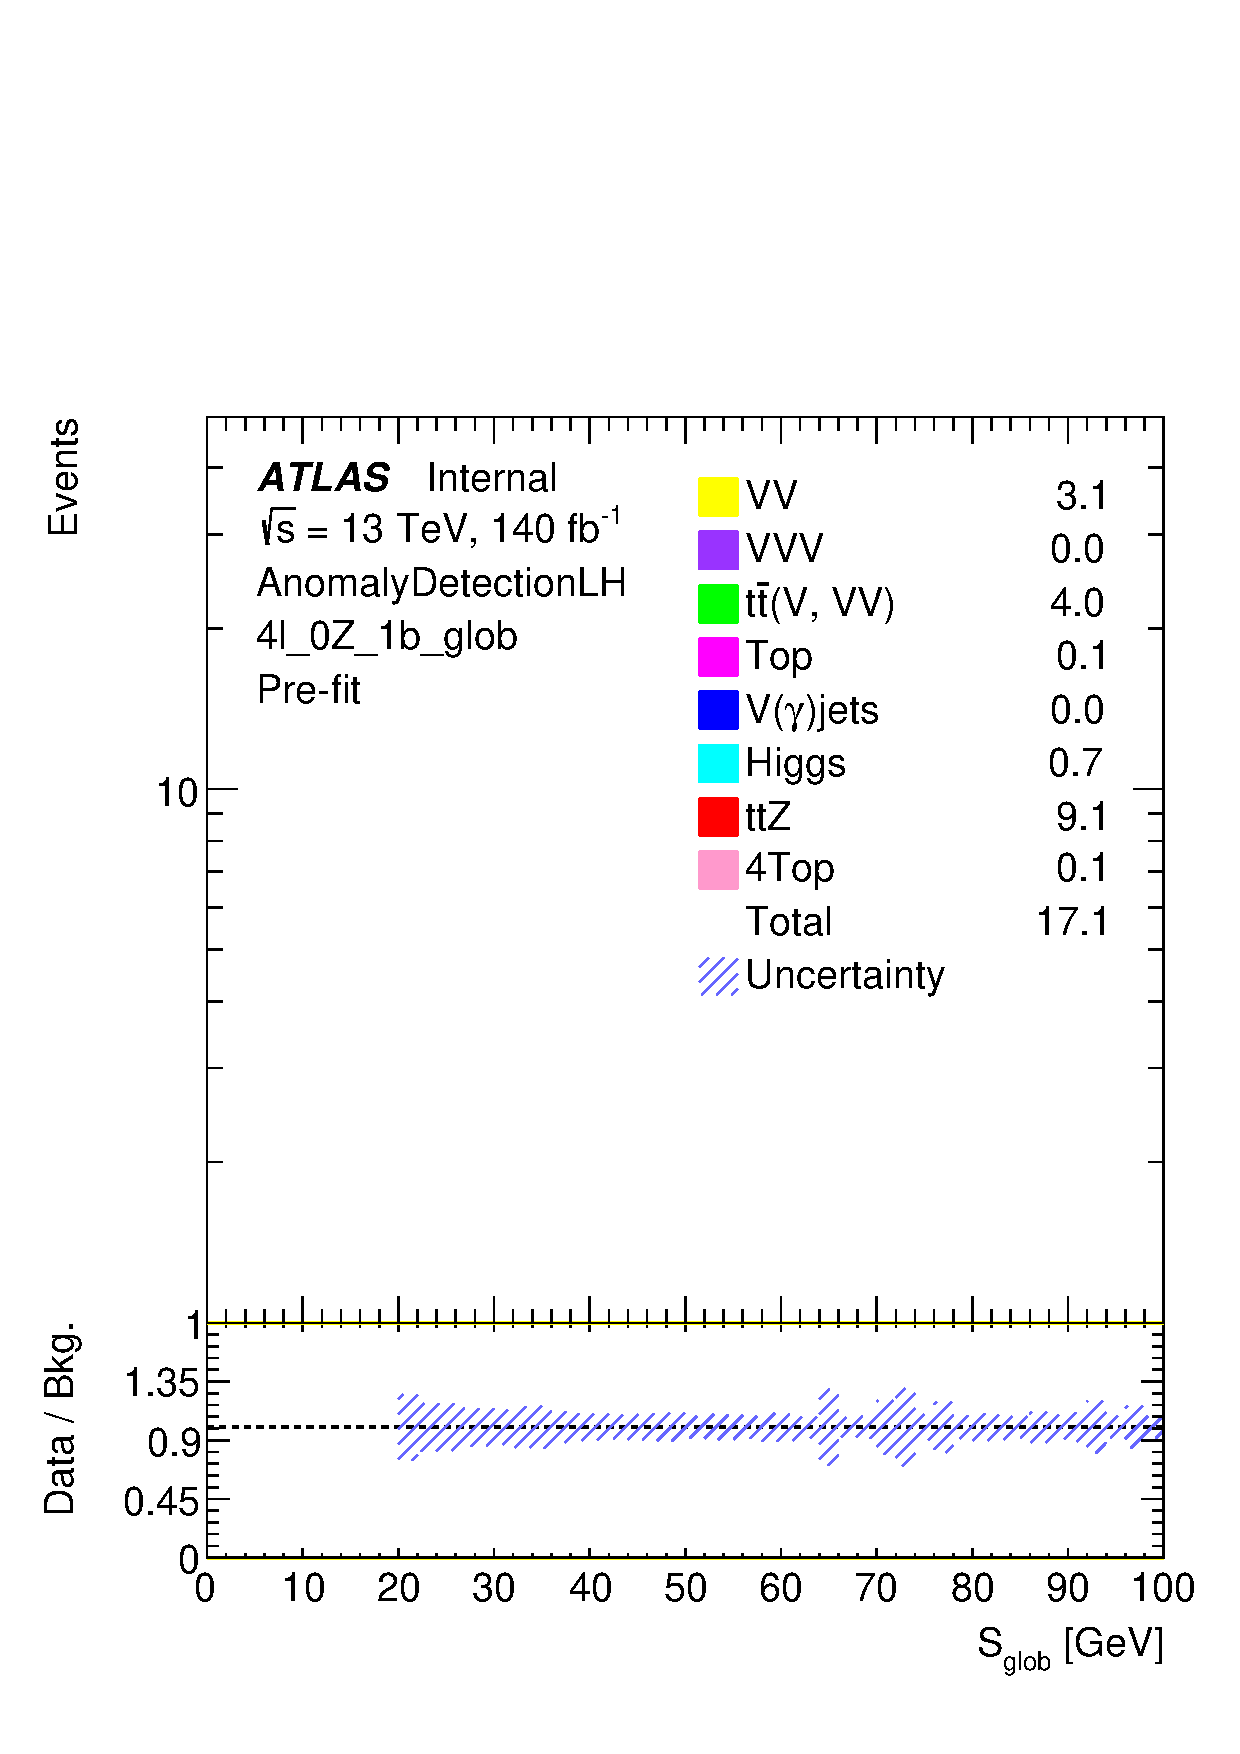
\includegraphics[width=0.24\textwidth]{plots/fourlepLH_run2/Plots/reg_4l_0Z_1b_glob_Zscore_glob.pdf}&
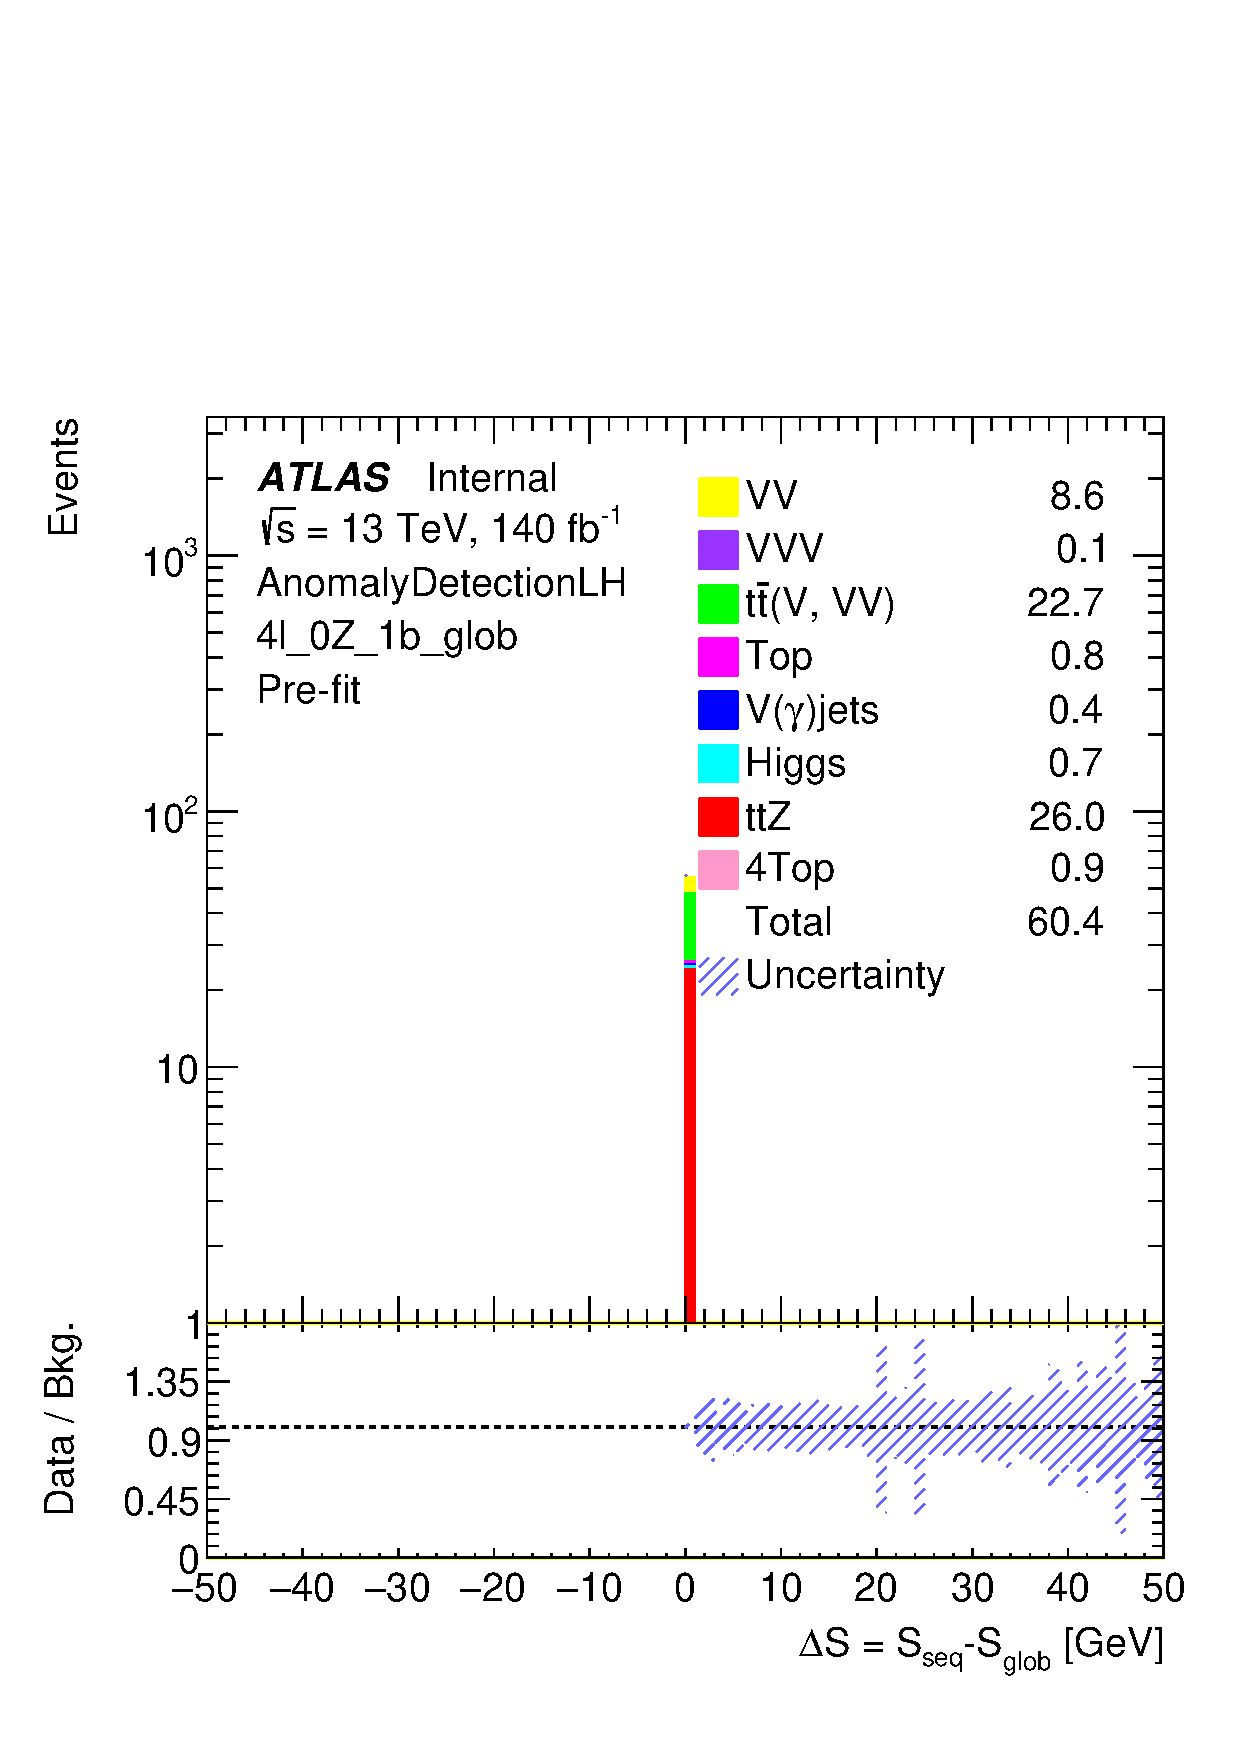
\includegraphics[width=0.24\textwidth]{plots/fourlepLH_run2/Plots/reg_4l_0Z_1b_glob_deltaZscore.pdf}
\end{tabular}
\end{frame}


\begin{frame}{\texttt{Results: 4l\_0Z\_1b}}
\begin{tabular}{cccccc}

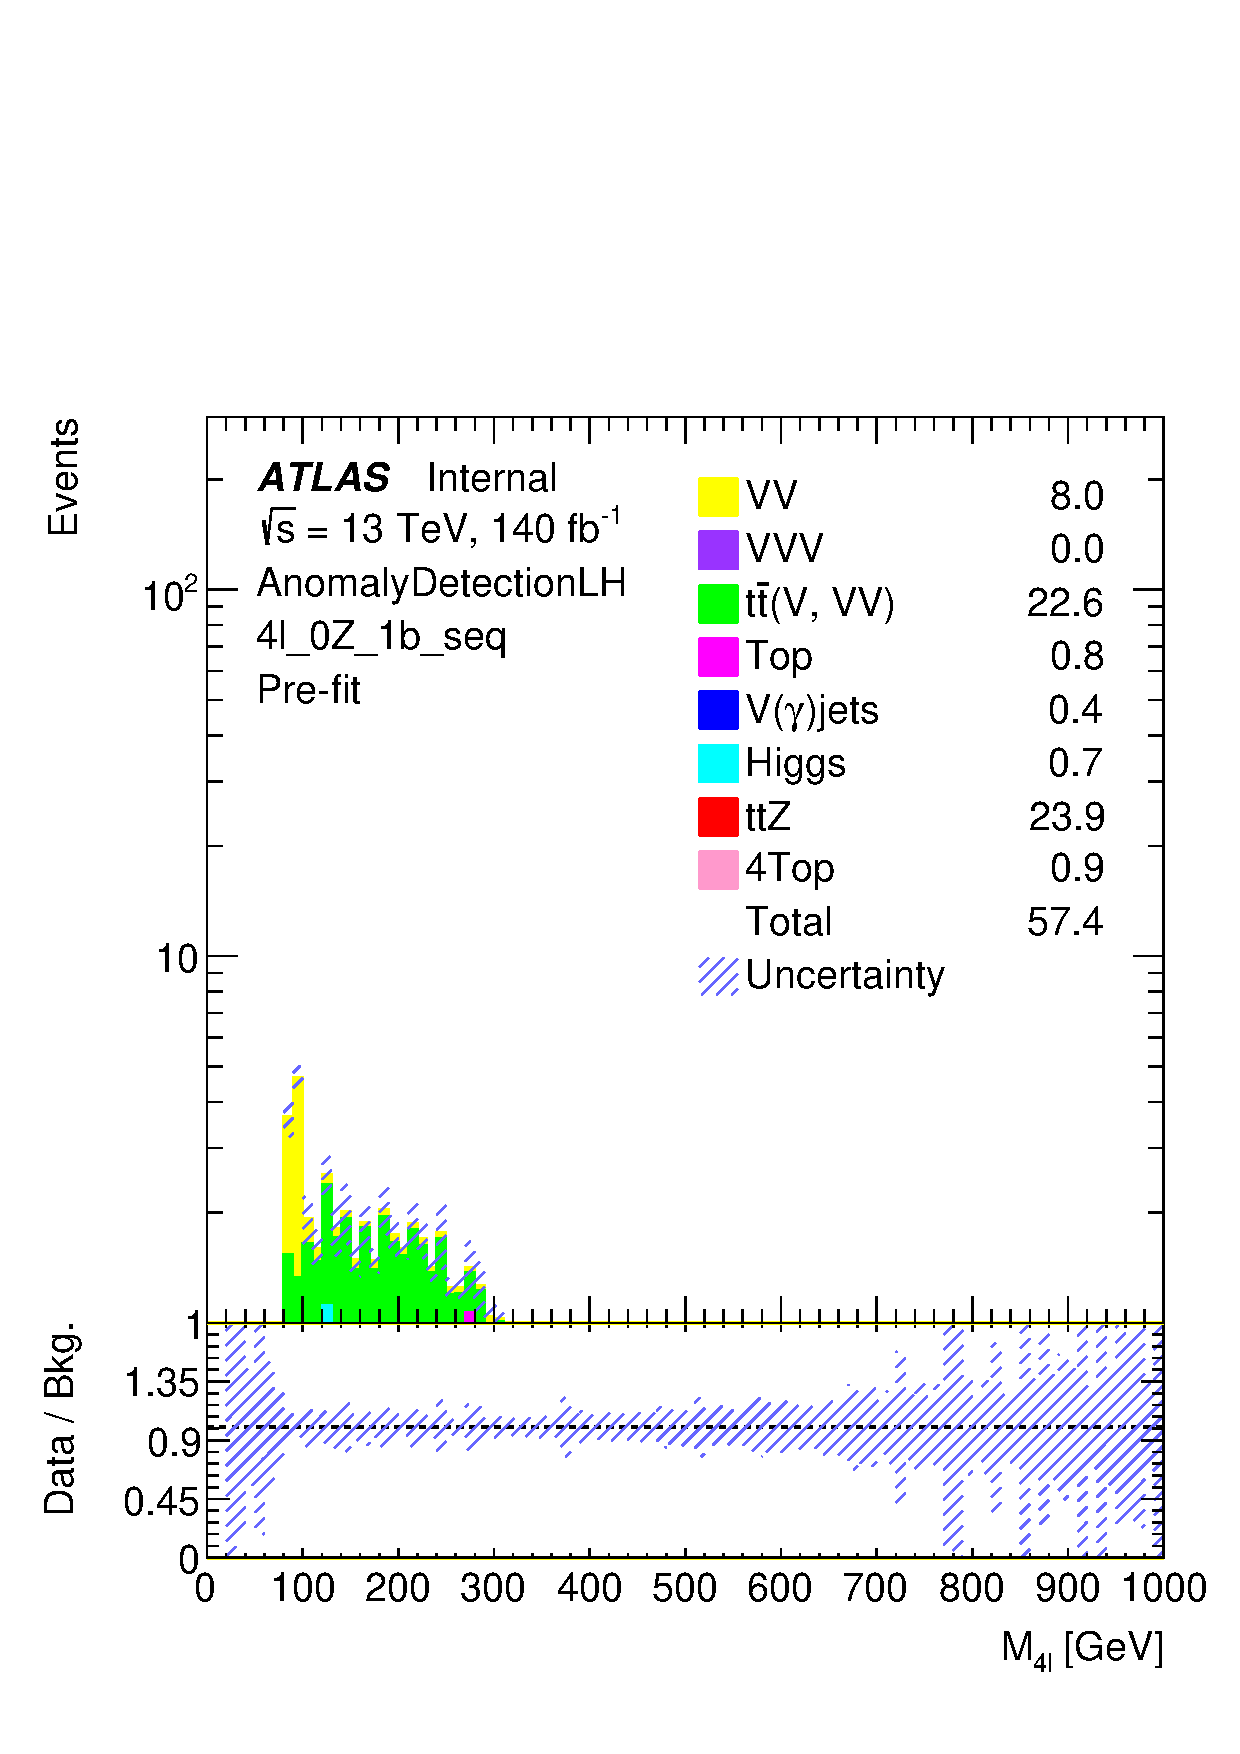
\includegraphics[width=0.24\textwidth]{plots/fourlepLH_run2/Plots/reg_4l_0Z_1b_seq_m4l.pdf} &
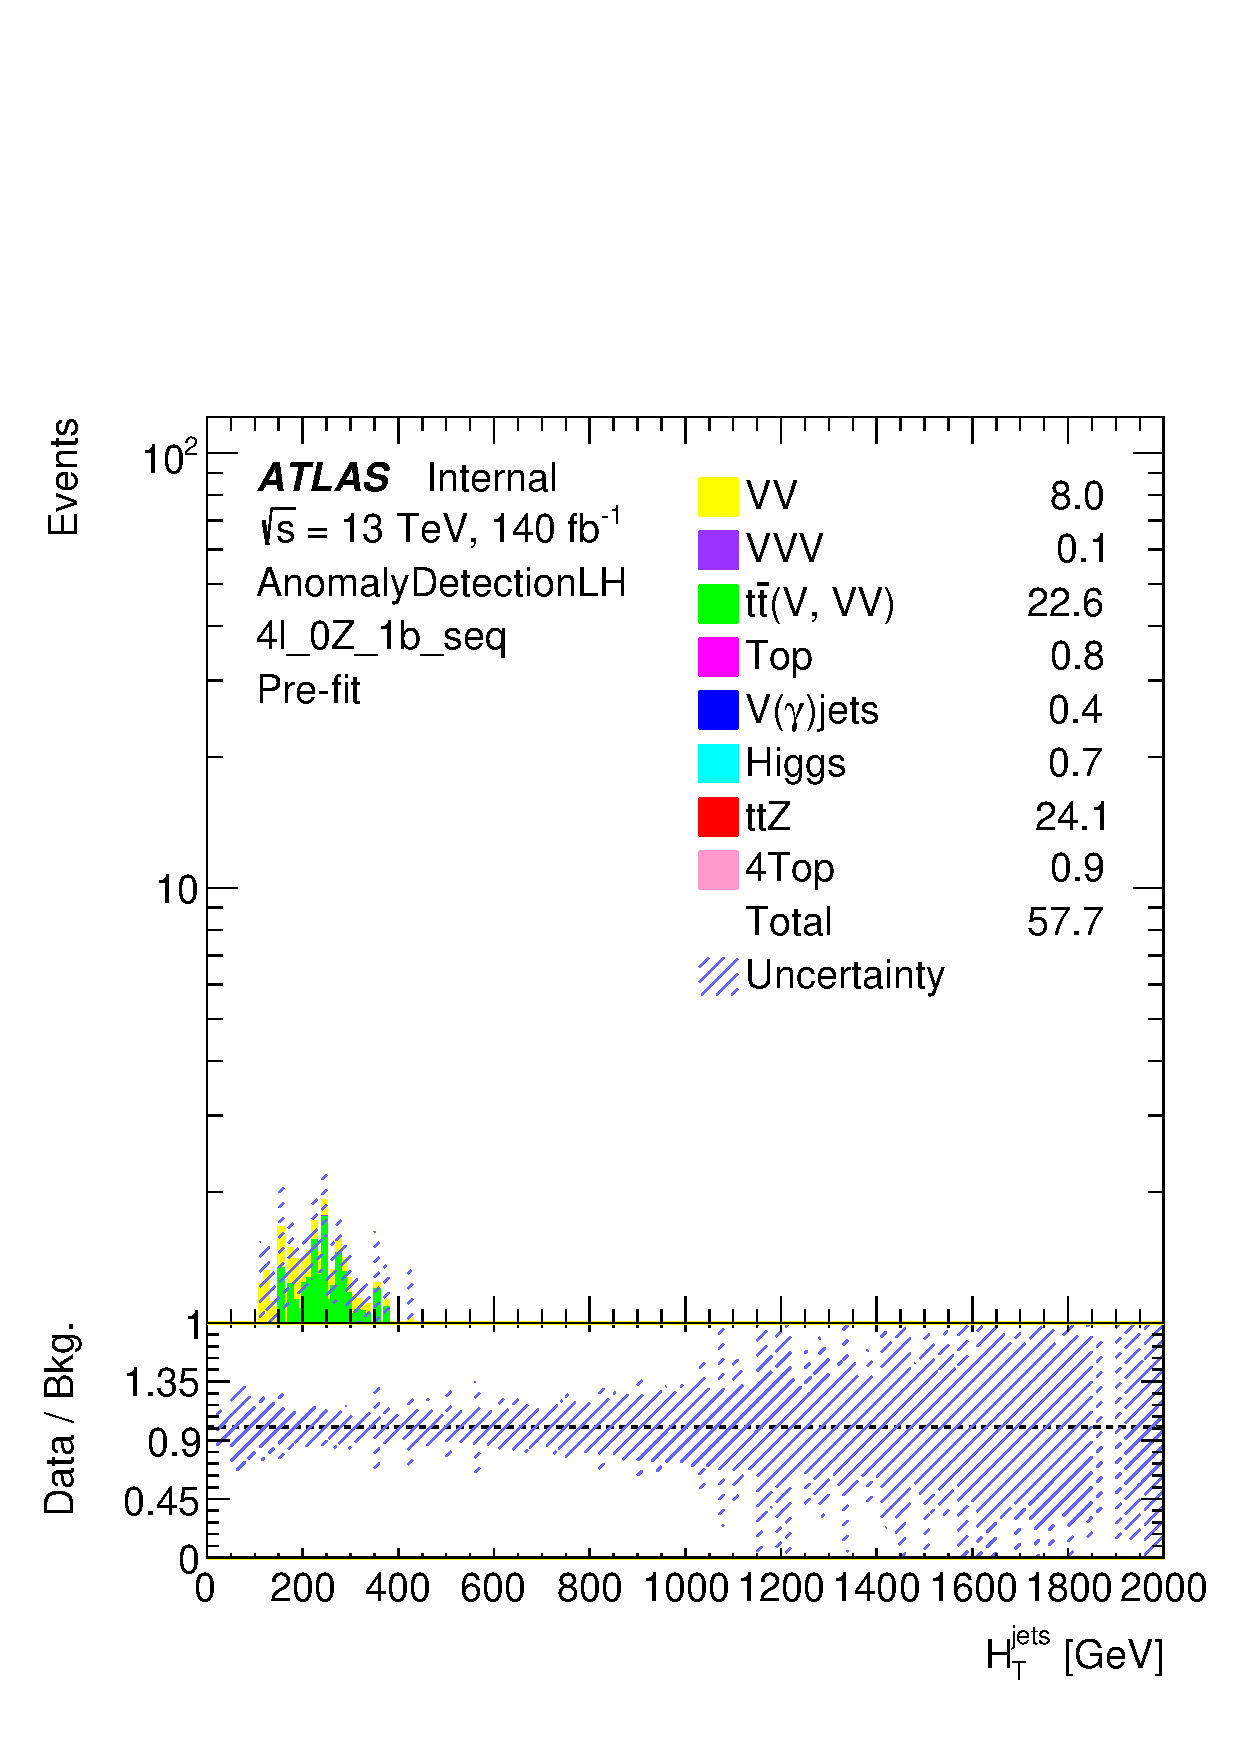
\includegraphics[width=0.24\textwidth]{plots/fourlepLH_run2/Plots/reg_4l_0Z_1b_seq_HT_jets.pdf} &
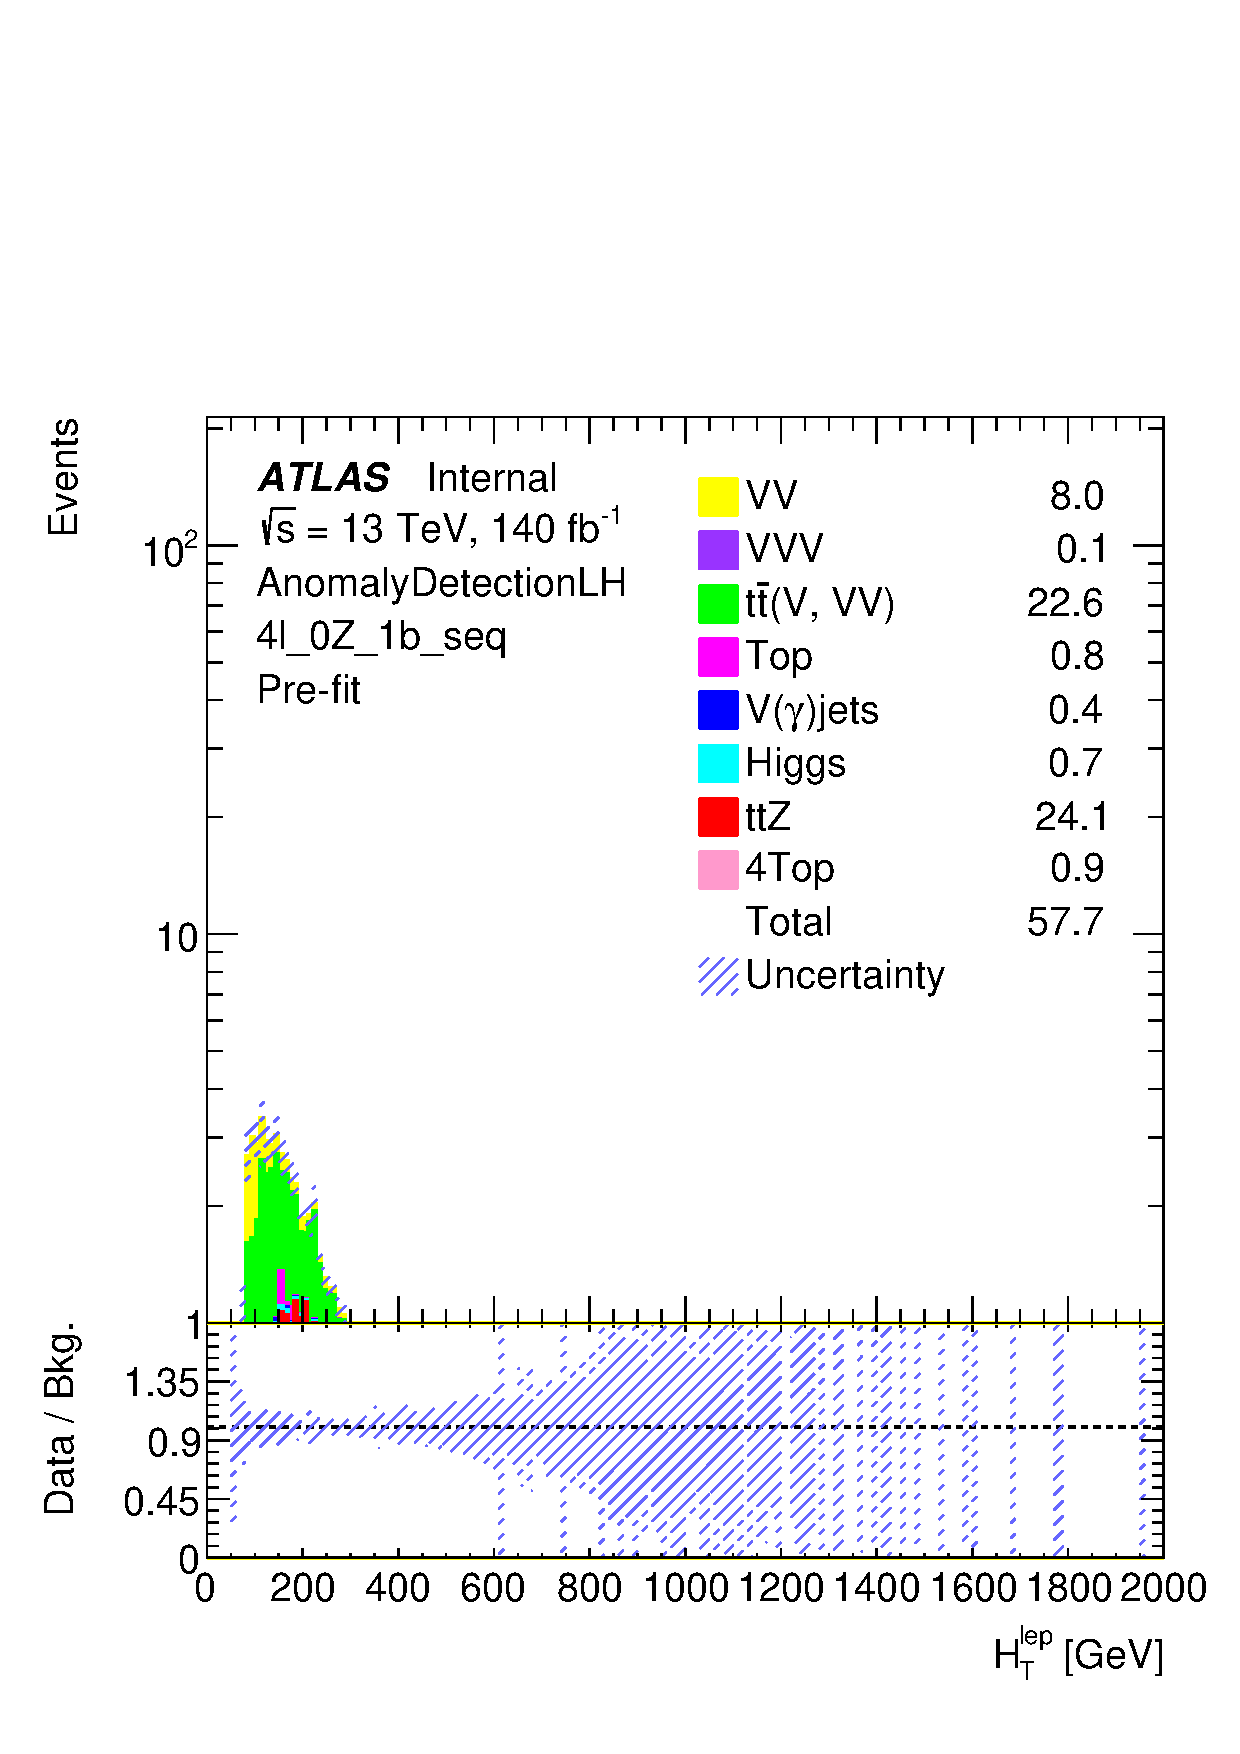
\includegraphics[width=0.24\textwidth]{plots/fourlepLH_run2/Plots/reg_4l_0Z_1b_seq_HT_lep.pdf} &
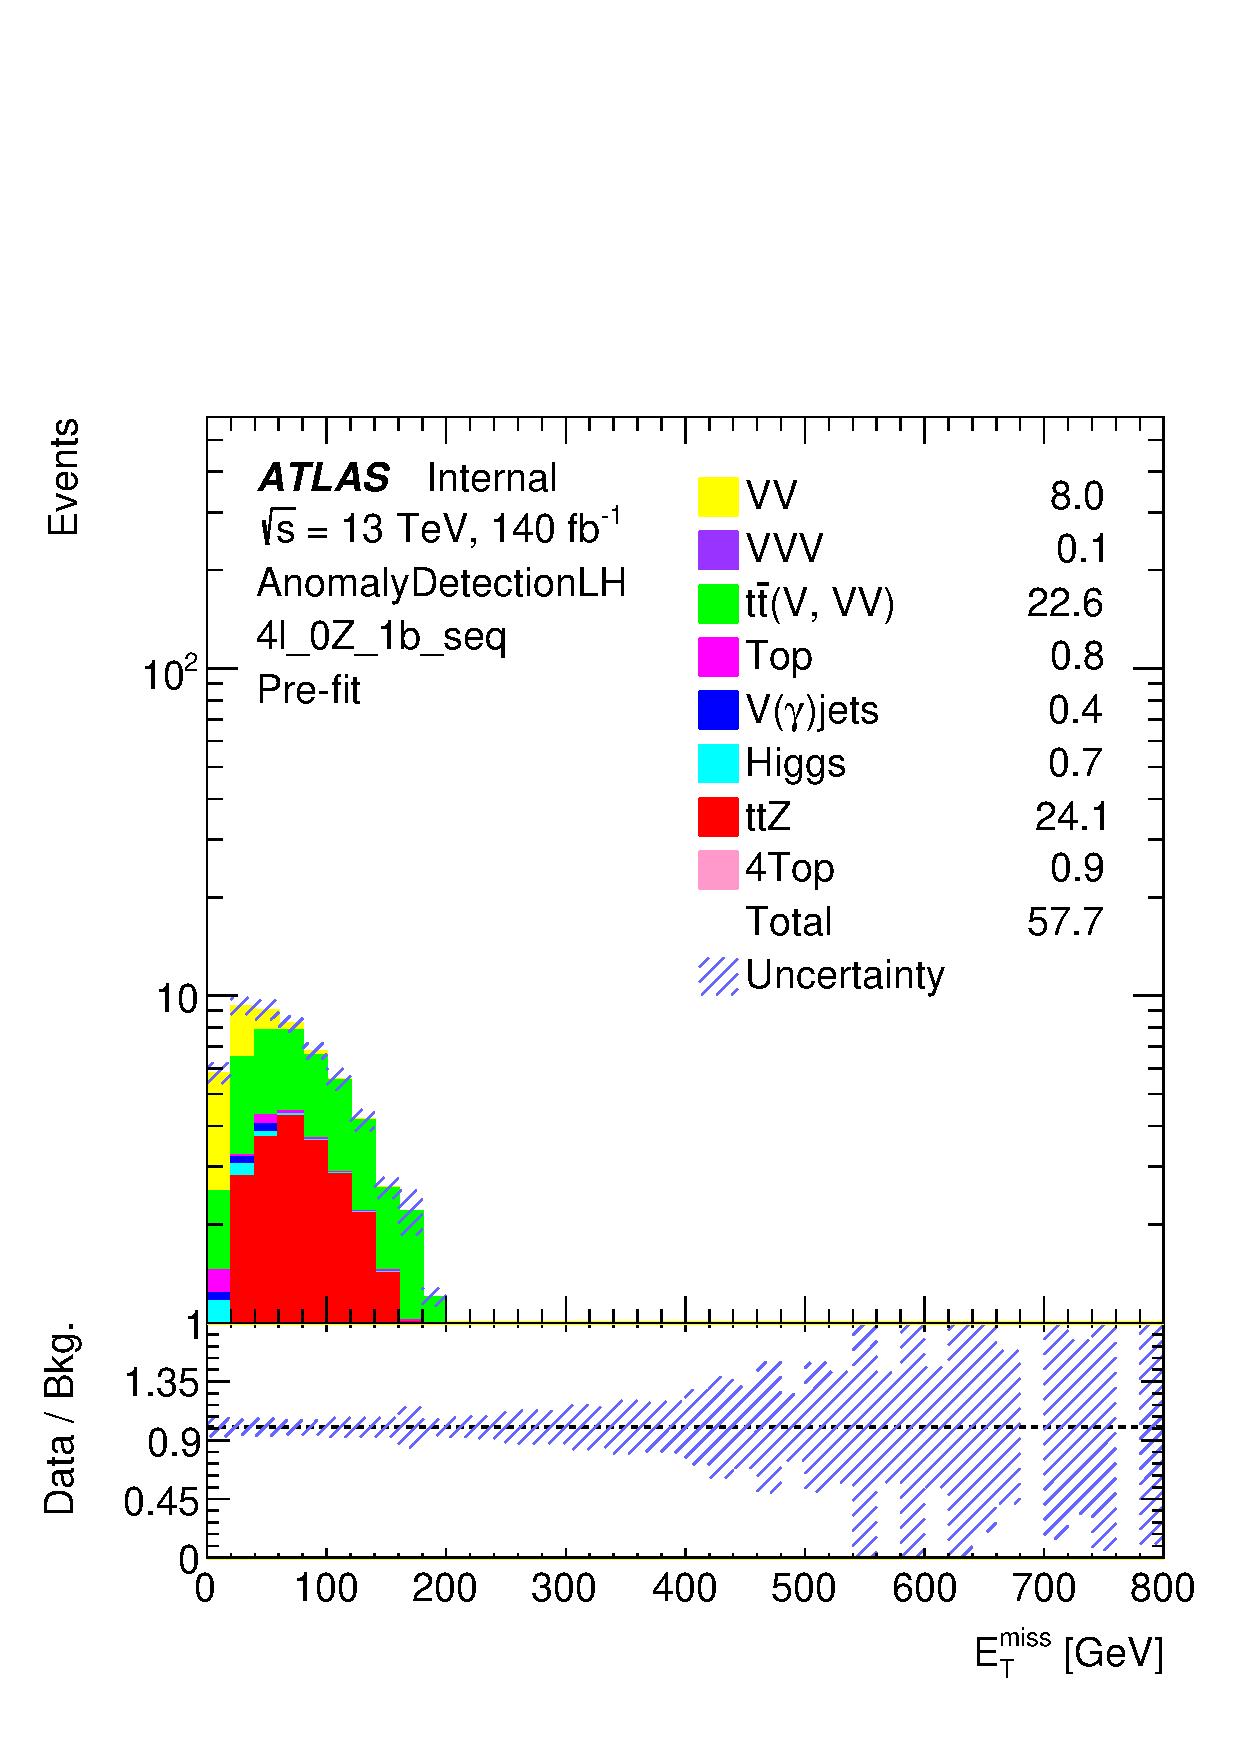
\includegraphics[width=0.24\textwidth]{plots/fourlepLH_run2/Plots/reg_4l_0Z_1b_seq_met.pdf} \\

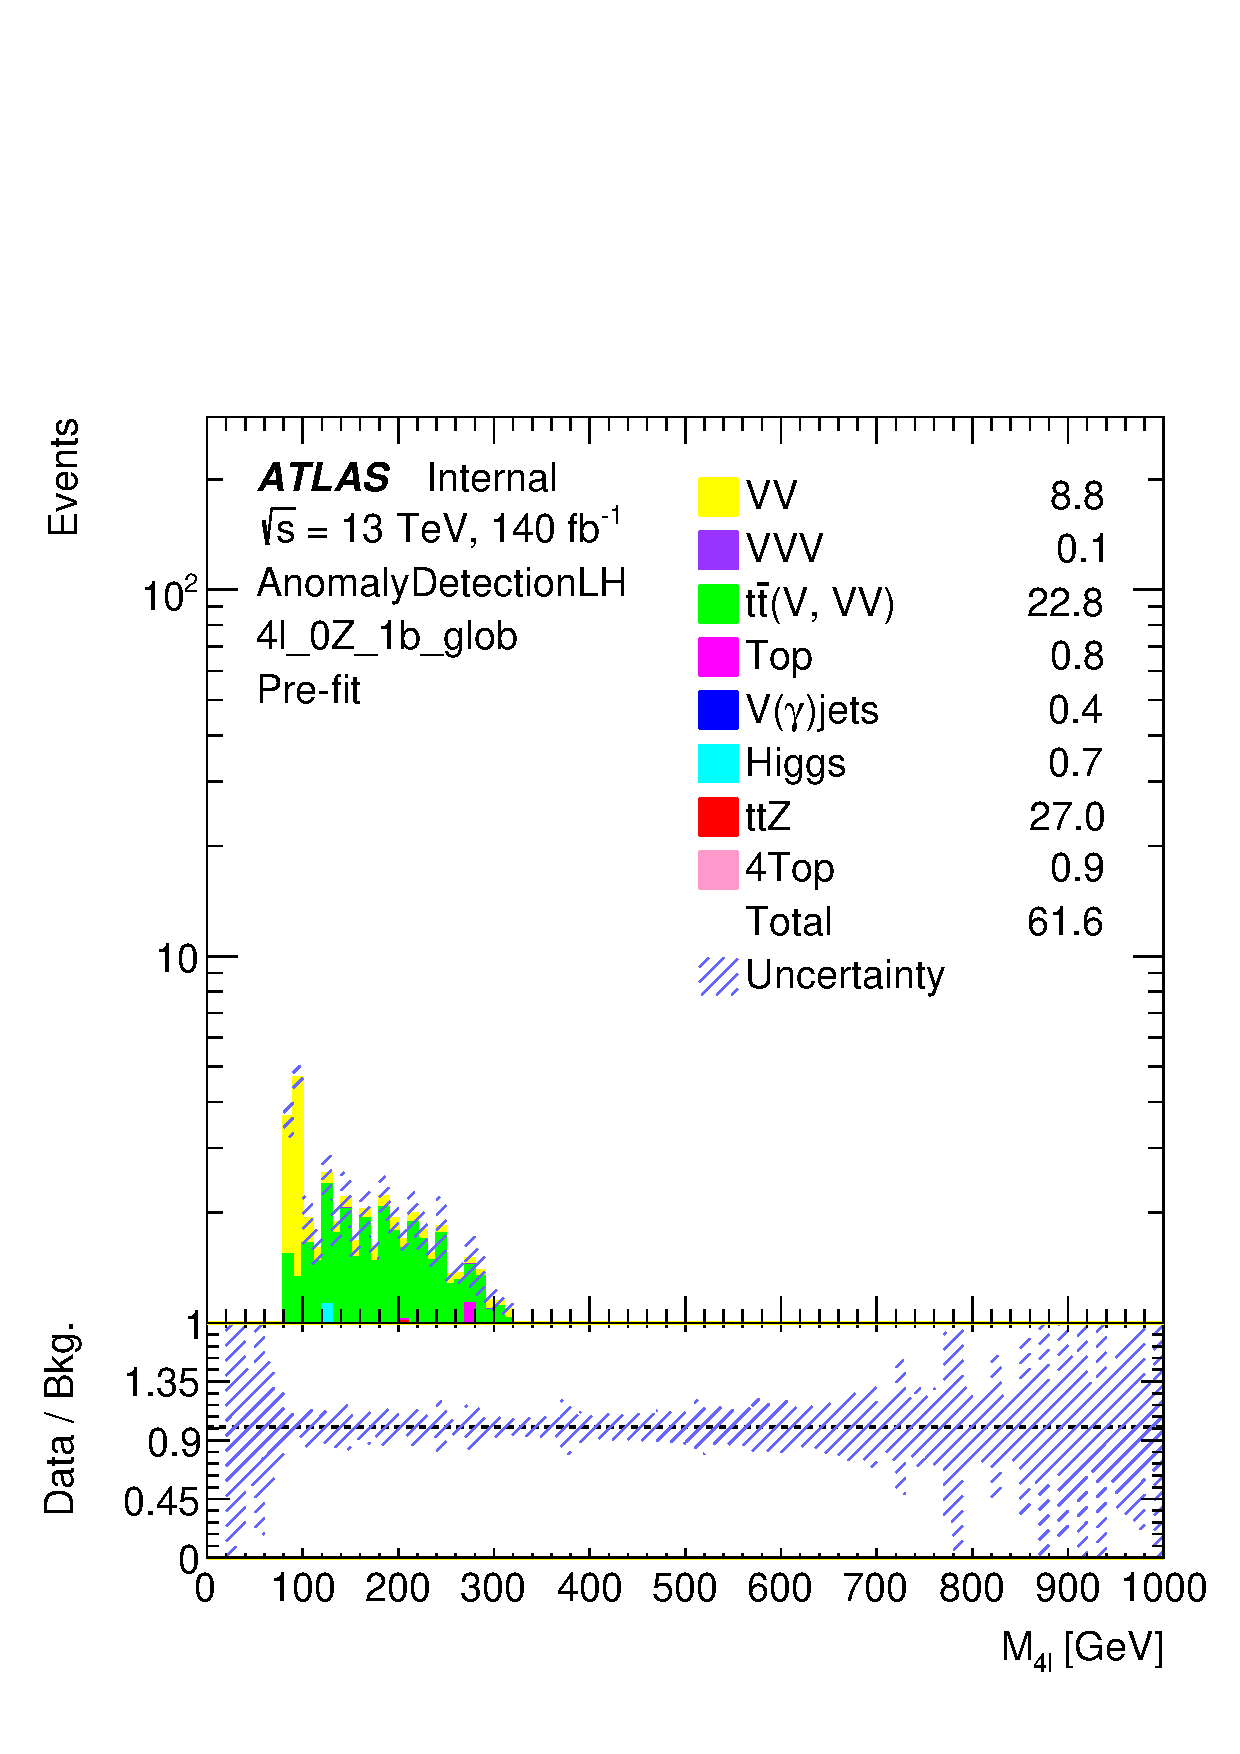
\includegraphics[width=0.24\textwidth]{plots/fourlepLH_run2/Plots/reg_4l_0Z_1b_glob_m4l.pdf} &
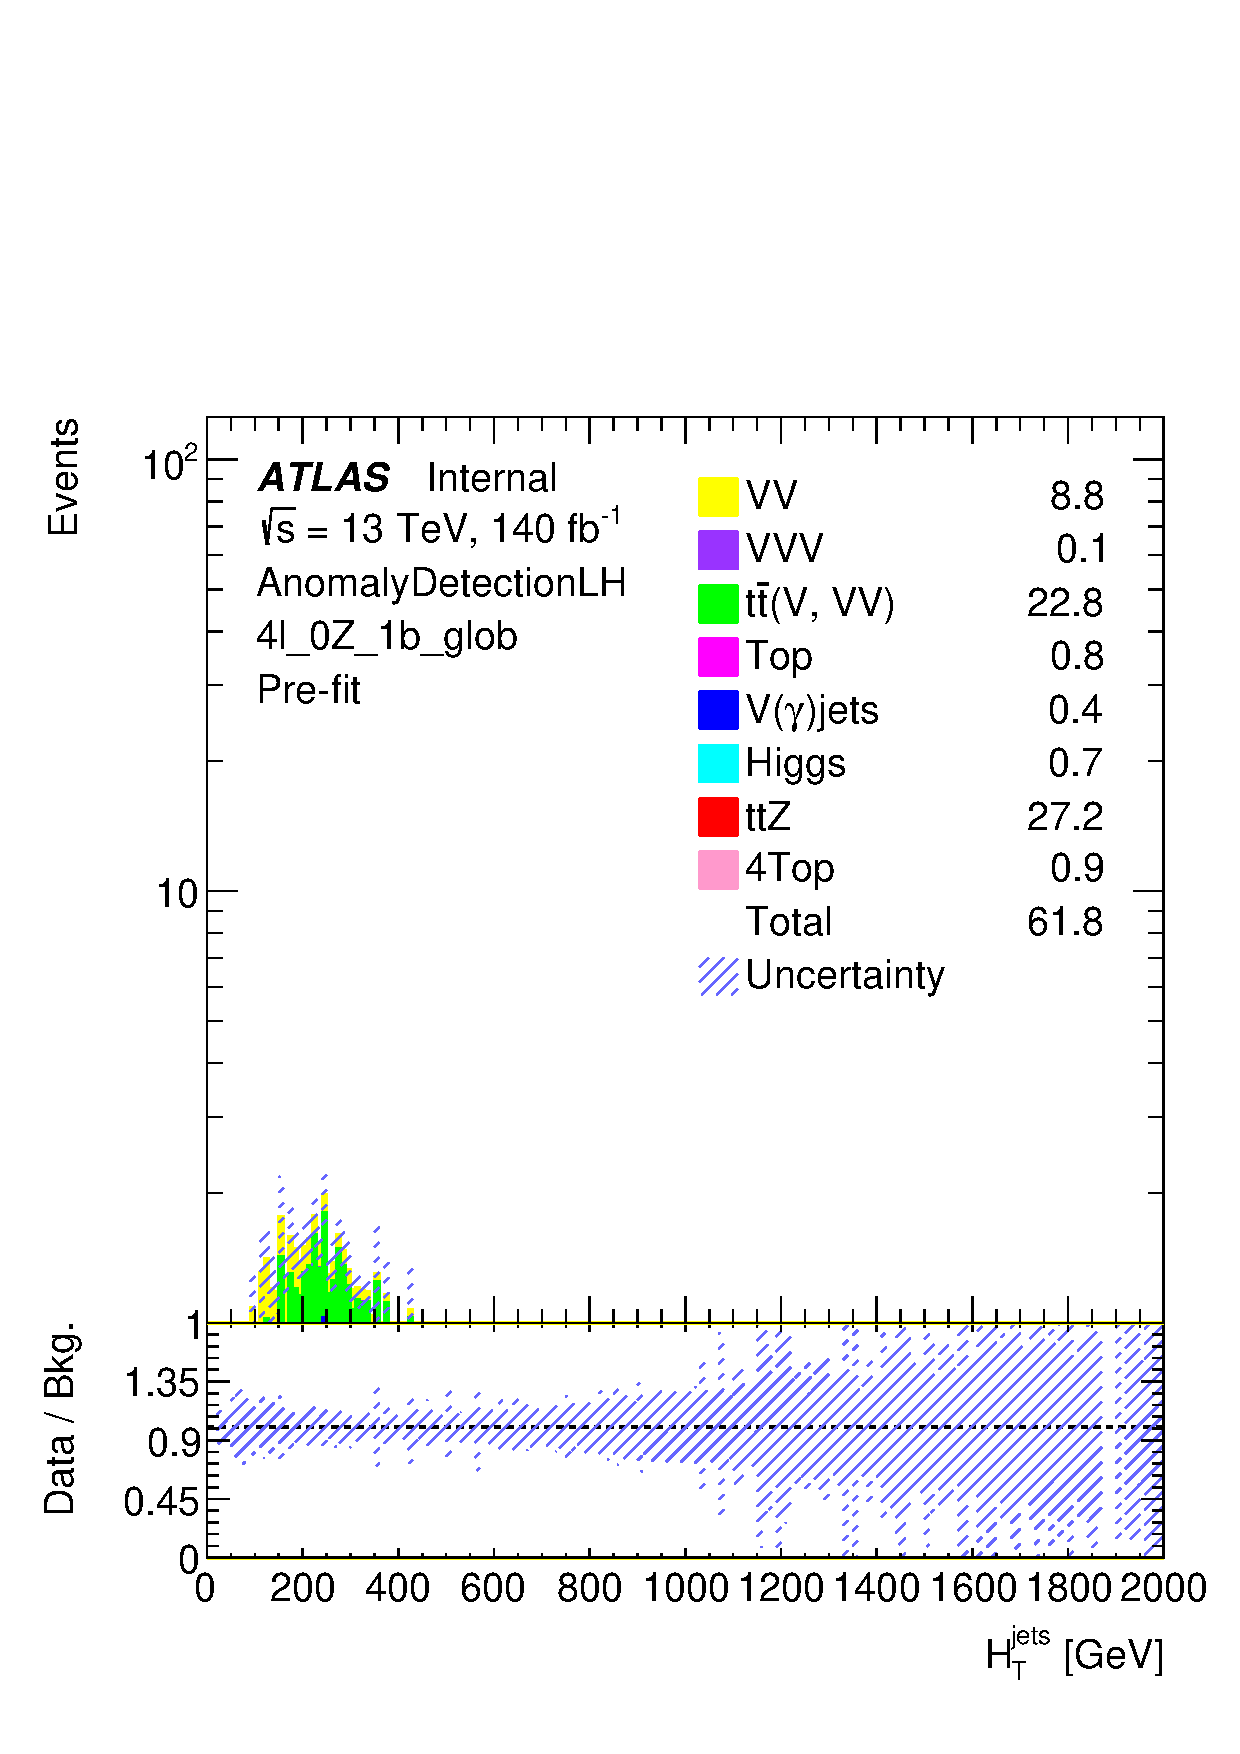
\includegraphics[width=0.24\textwidth]{plots/fourlepLH_run2/Plots/reg_4l_0Z_1b_glob_HT_jets.pdf} &
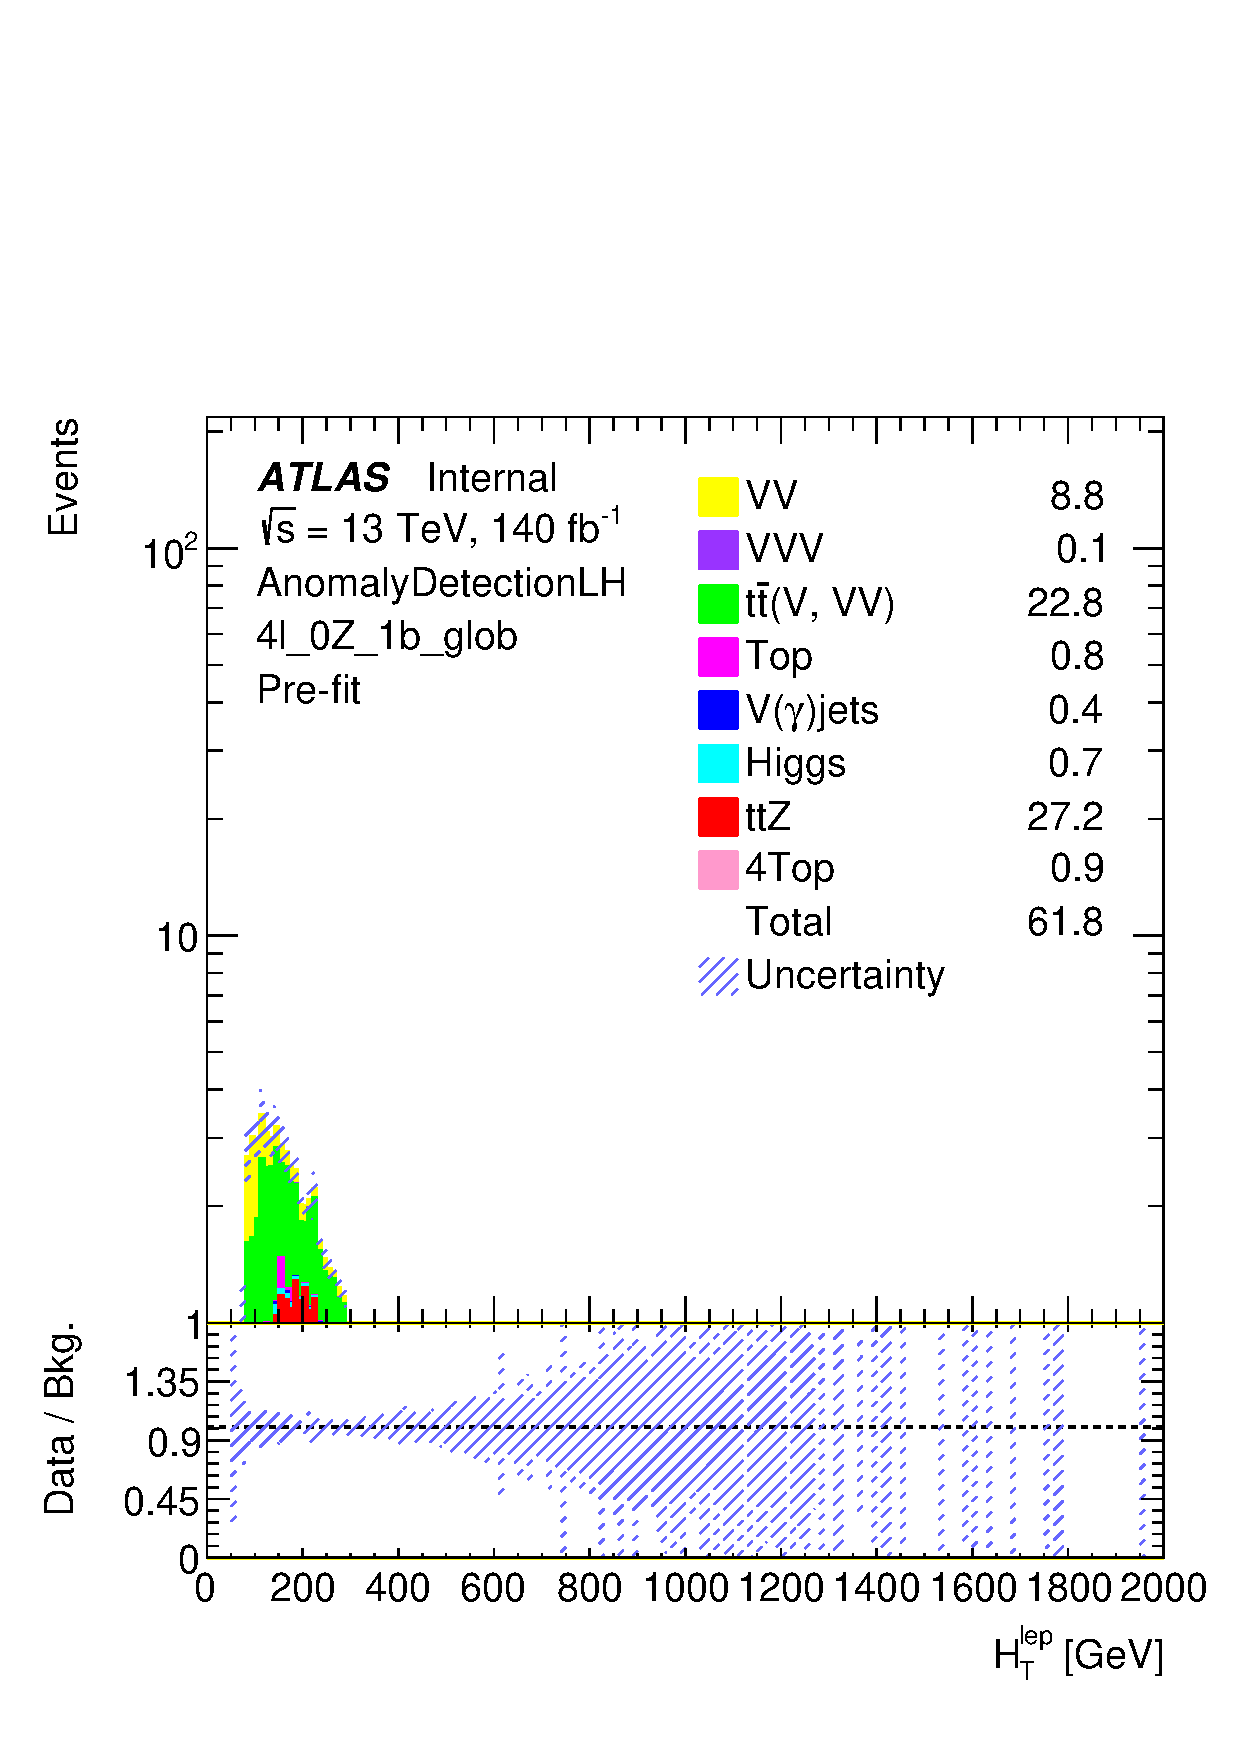
\includegraphics[width=0.24\textwidth]{plots/fourlepLH_run2/Plots/reg_4l_0Z_1b_glob_HT_lep.pdf} &
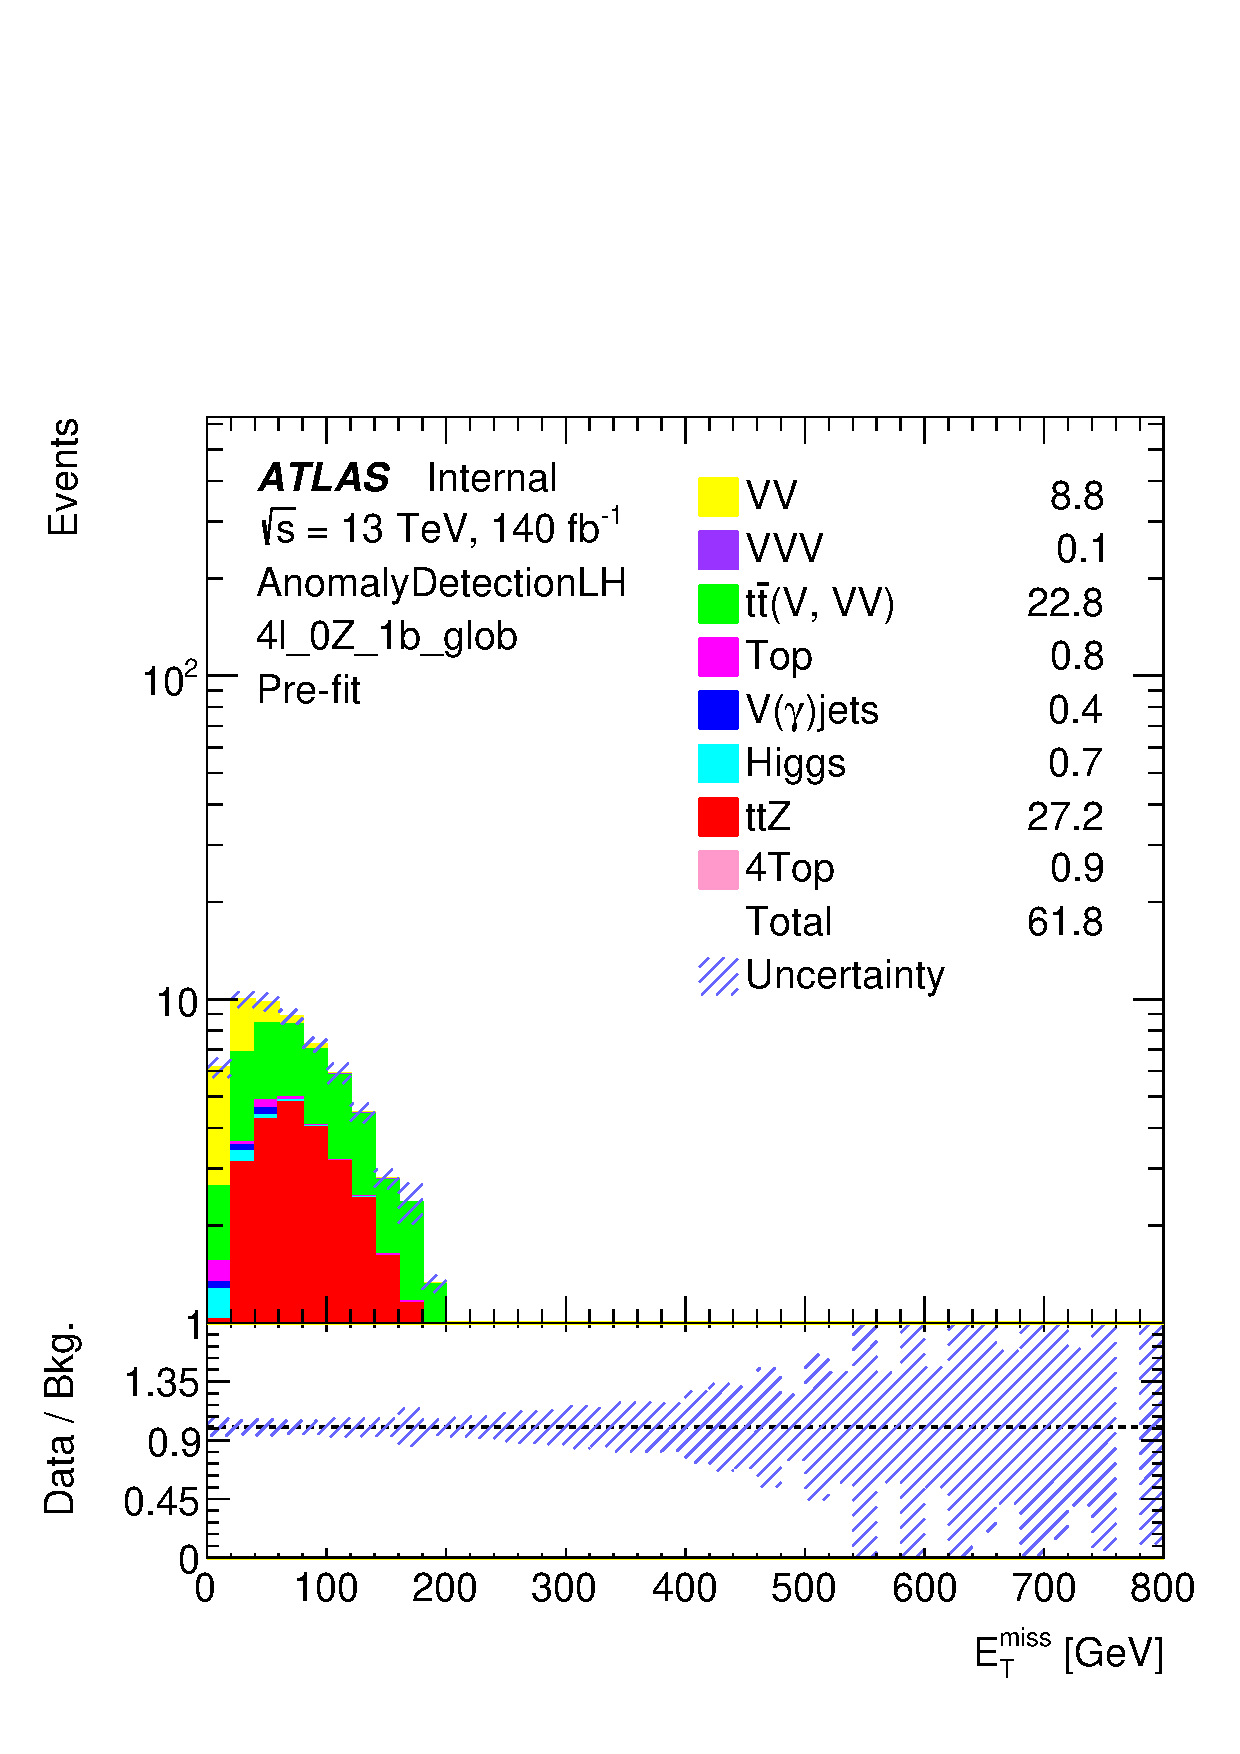
\includegraphics[width=0.24\textwidth]{plots/fourlepLH_run2/Plots/reg_4l_0Z_1b_glob_met.pdf} \\

\end{tabular}
\end{frame}

\begin{frame}{\texttt{Results: 4l\_0Z\_1b}}
\begin{tabular}{cccccc}
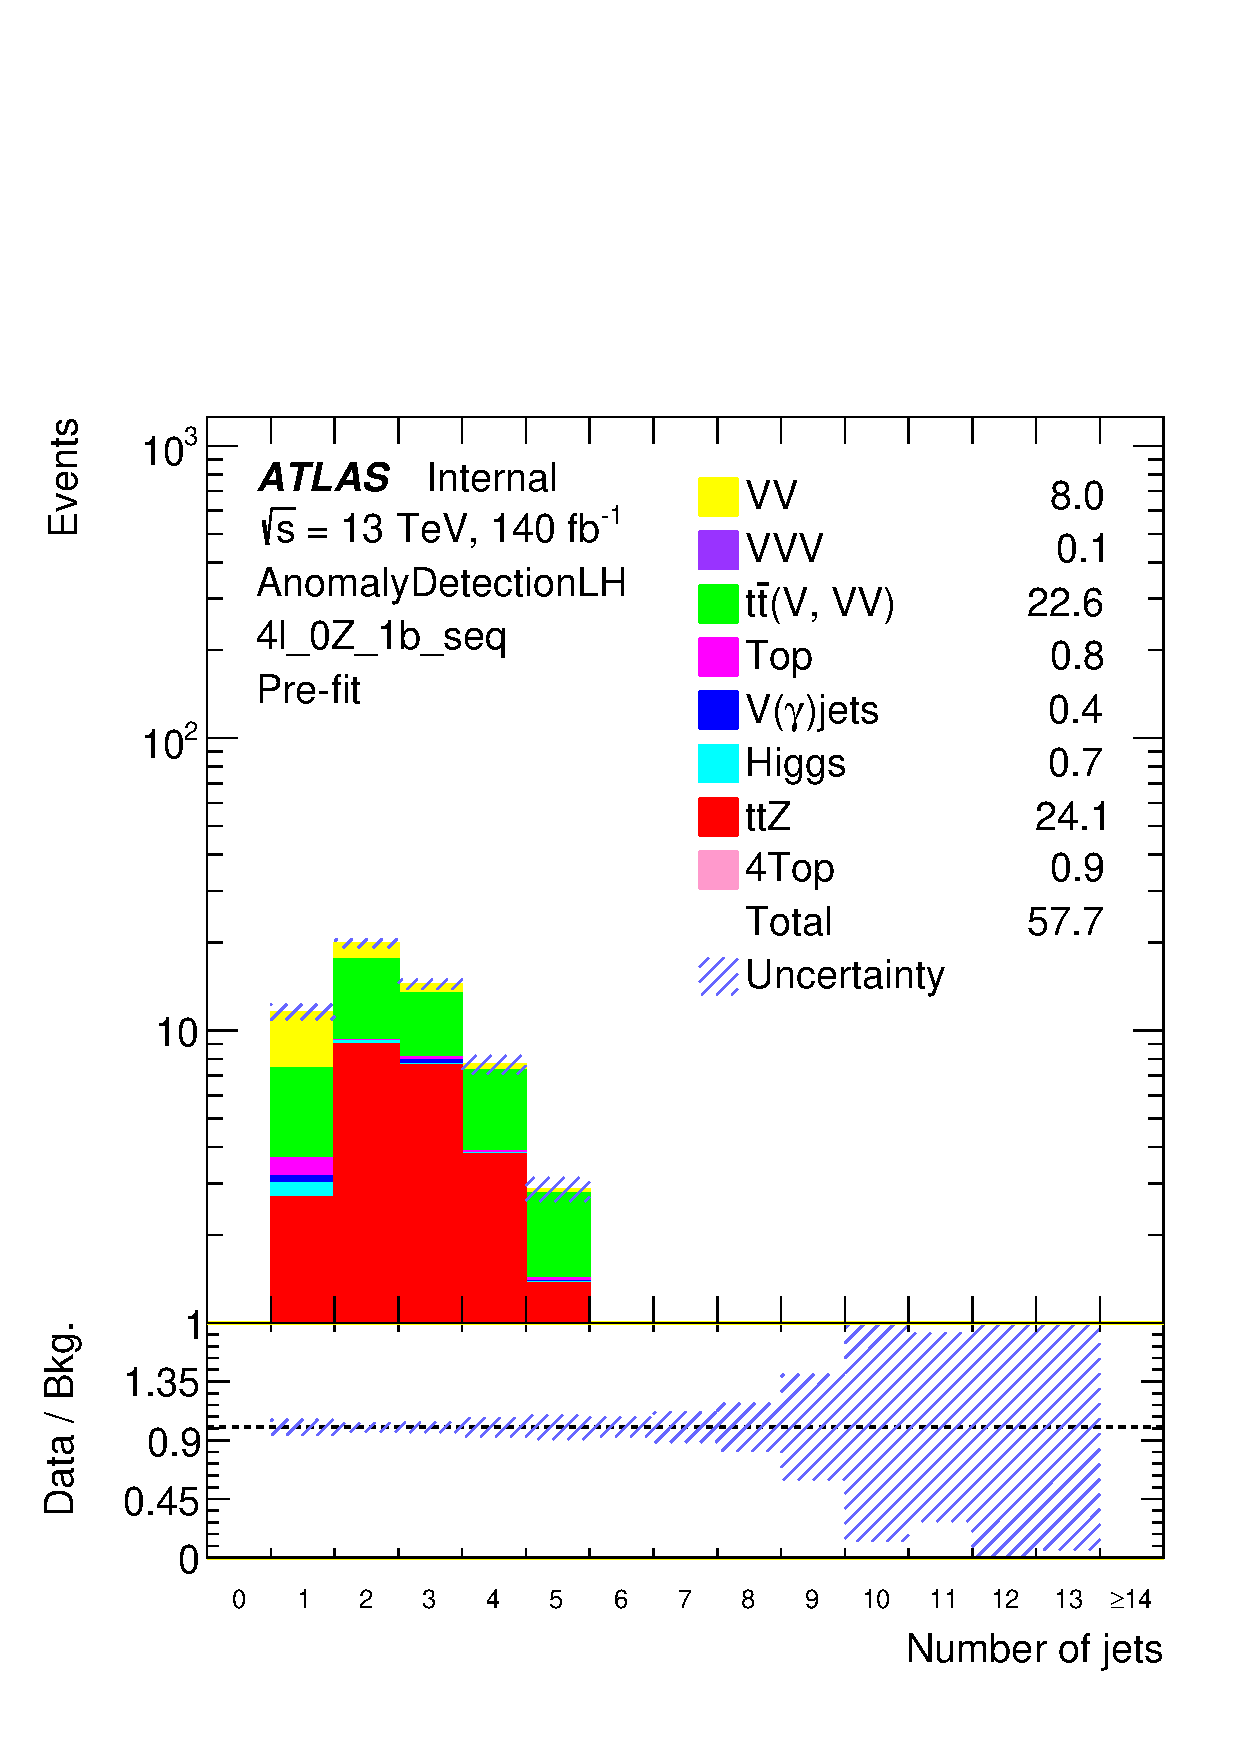
\includegraphics[width=0.24\textwidth]{plots/fourlepLH_run2/Plots/reg_4l_0Z_1b_seq_nJets.pdf} &
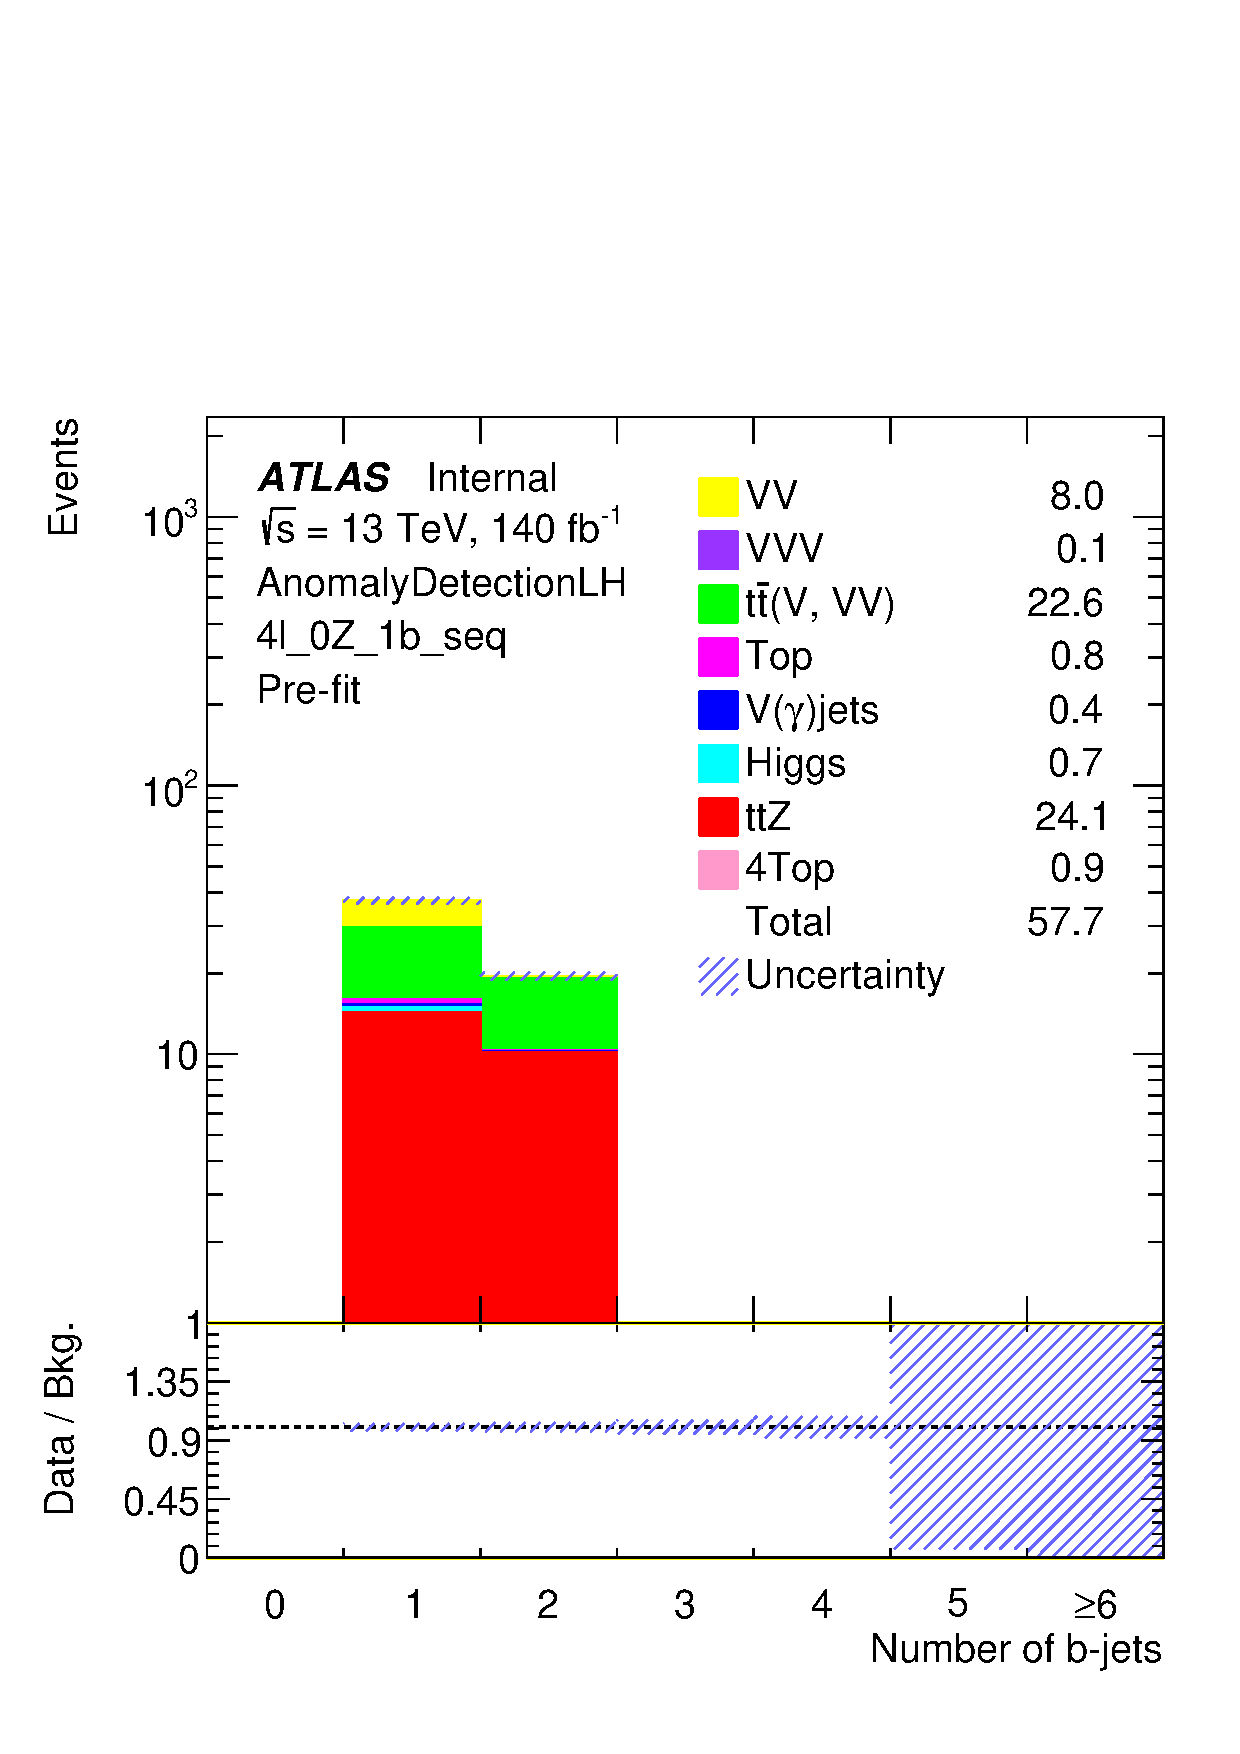
\includegraphics[width=0.24\textwidth]{plots/fourlepLH_run2/Plots/reg_4l_0Z_1b_seq_nbJets.pdf} &
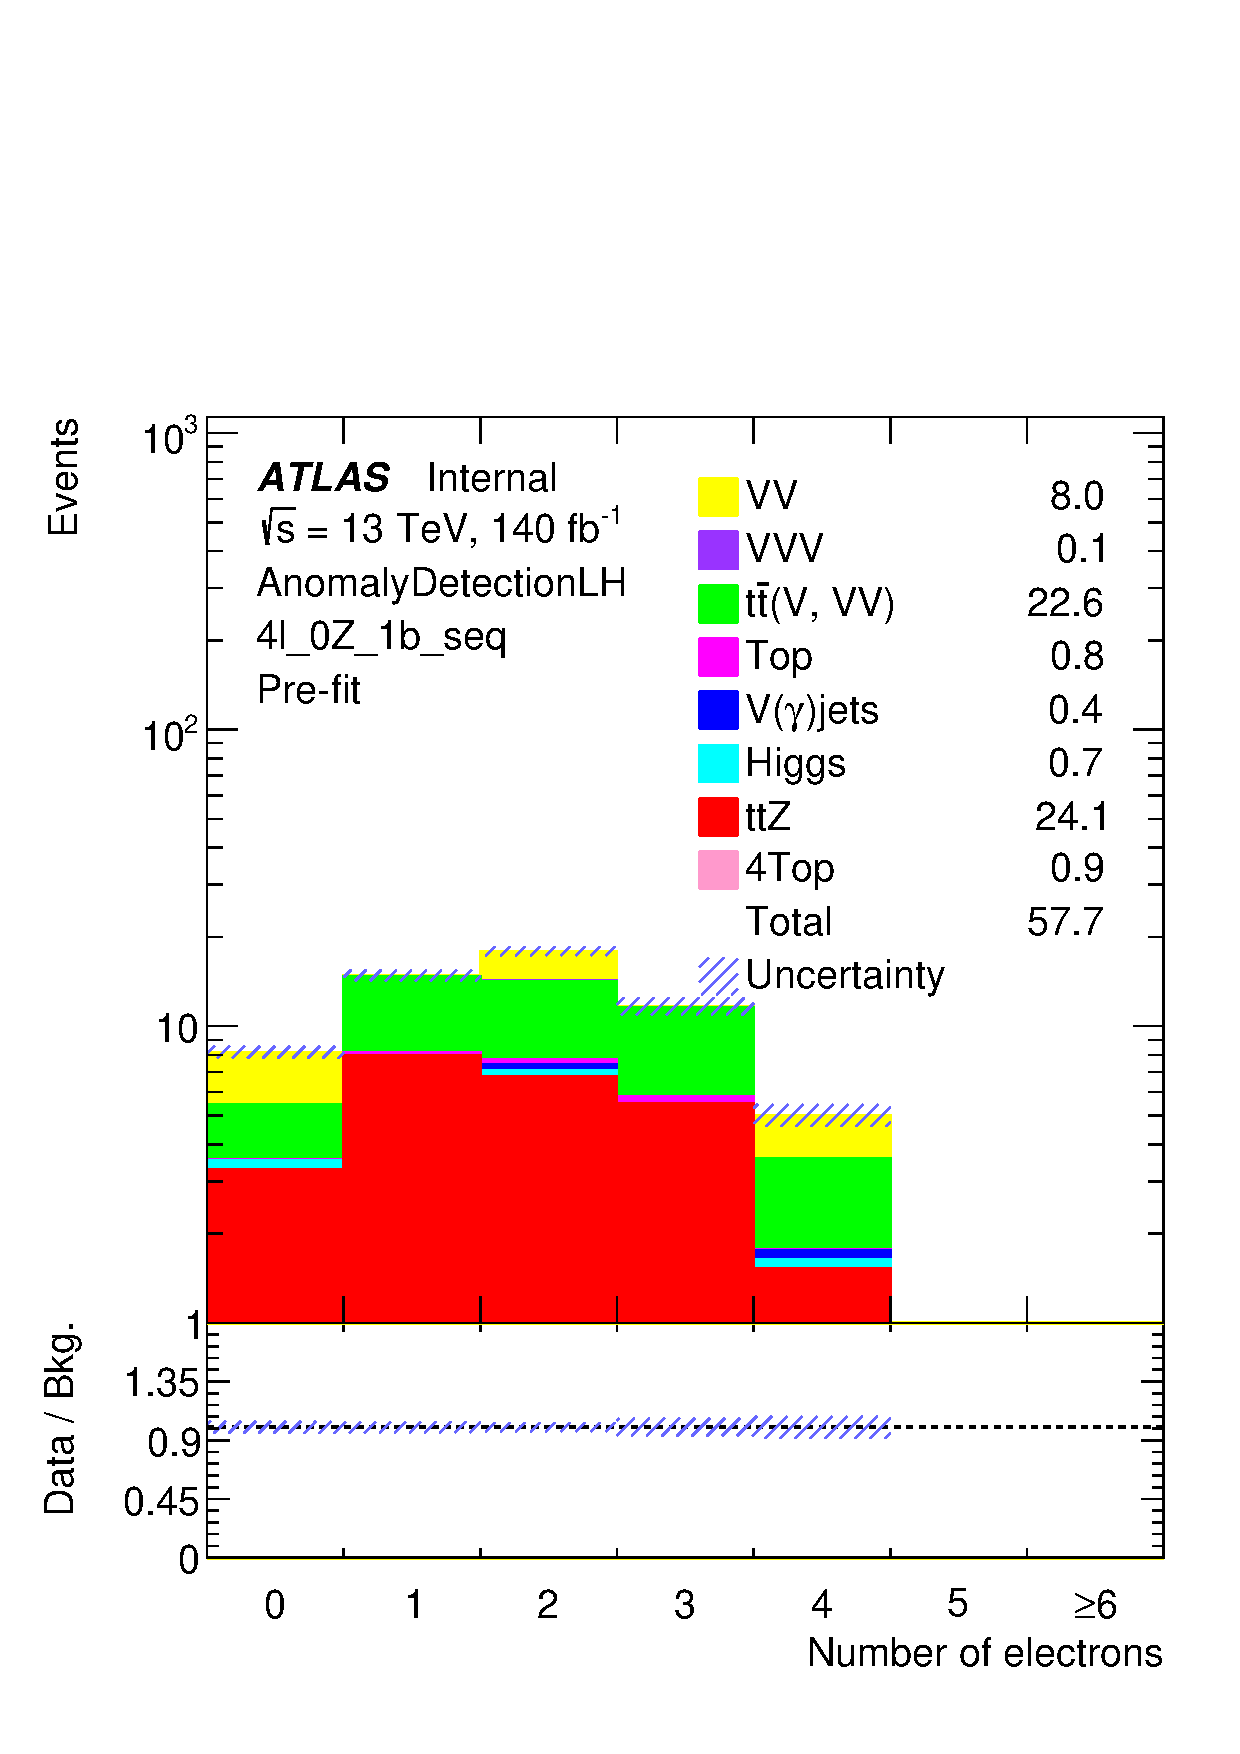
\includegraphics[width=0.24\textwidth]{plots/fourlepLH_run2/Plots/reg_4l_0Z_1b_seq_nElectrons.pdf} &
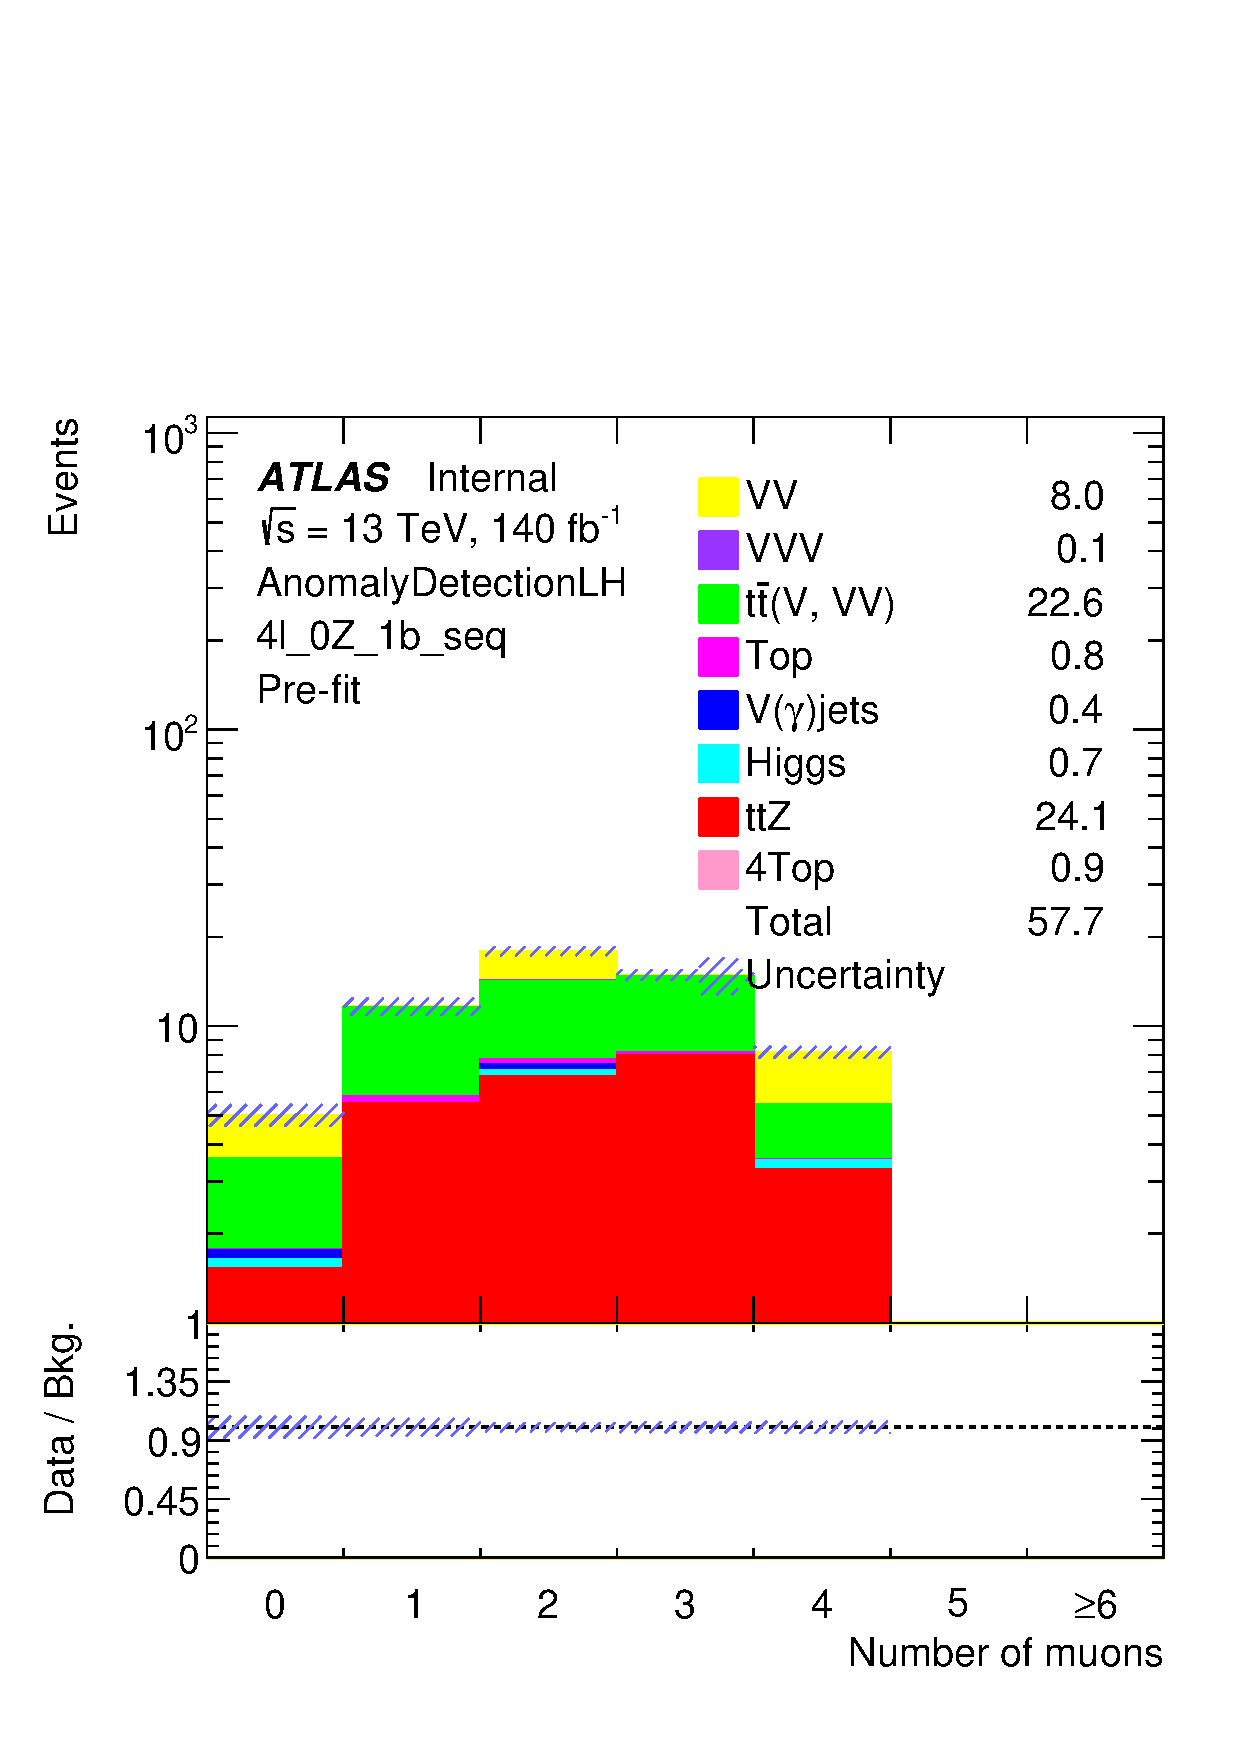
\includegraphics[width=0.24\textwidth]{plots/fourlepLH_run2/Plots/reg_4l_0Z_1b_seq_nMuons.pdf} \\

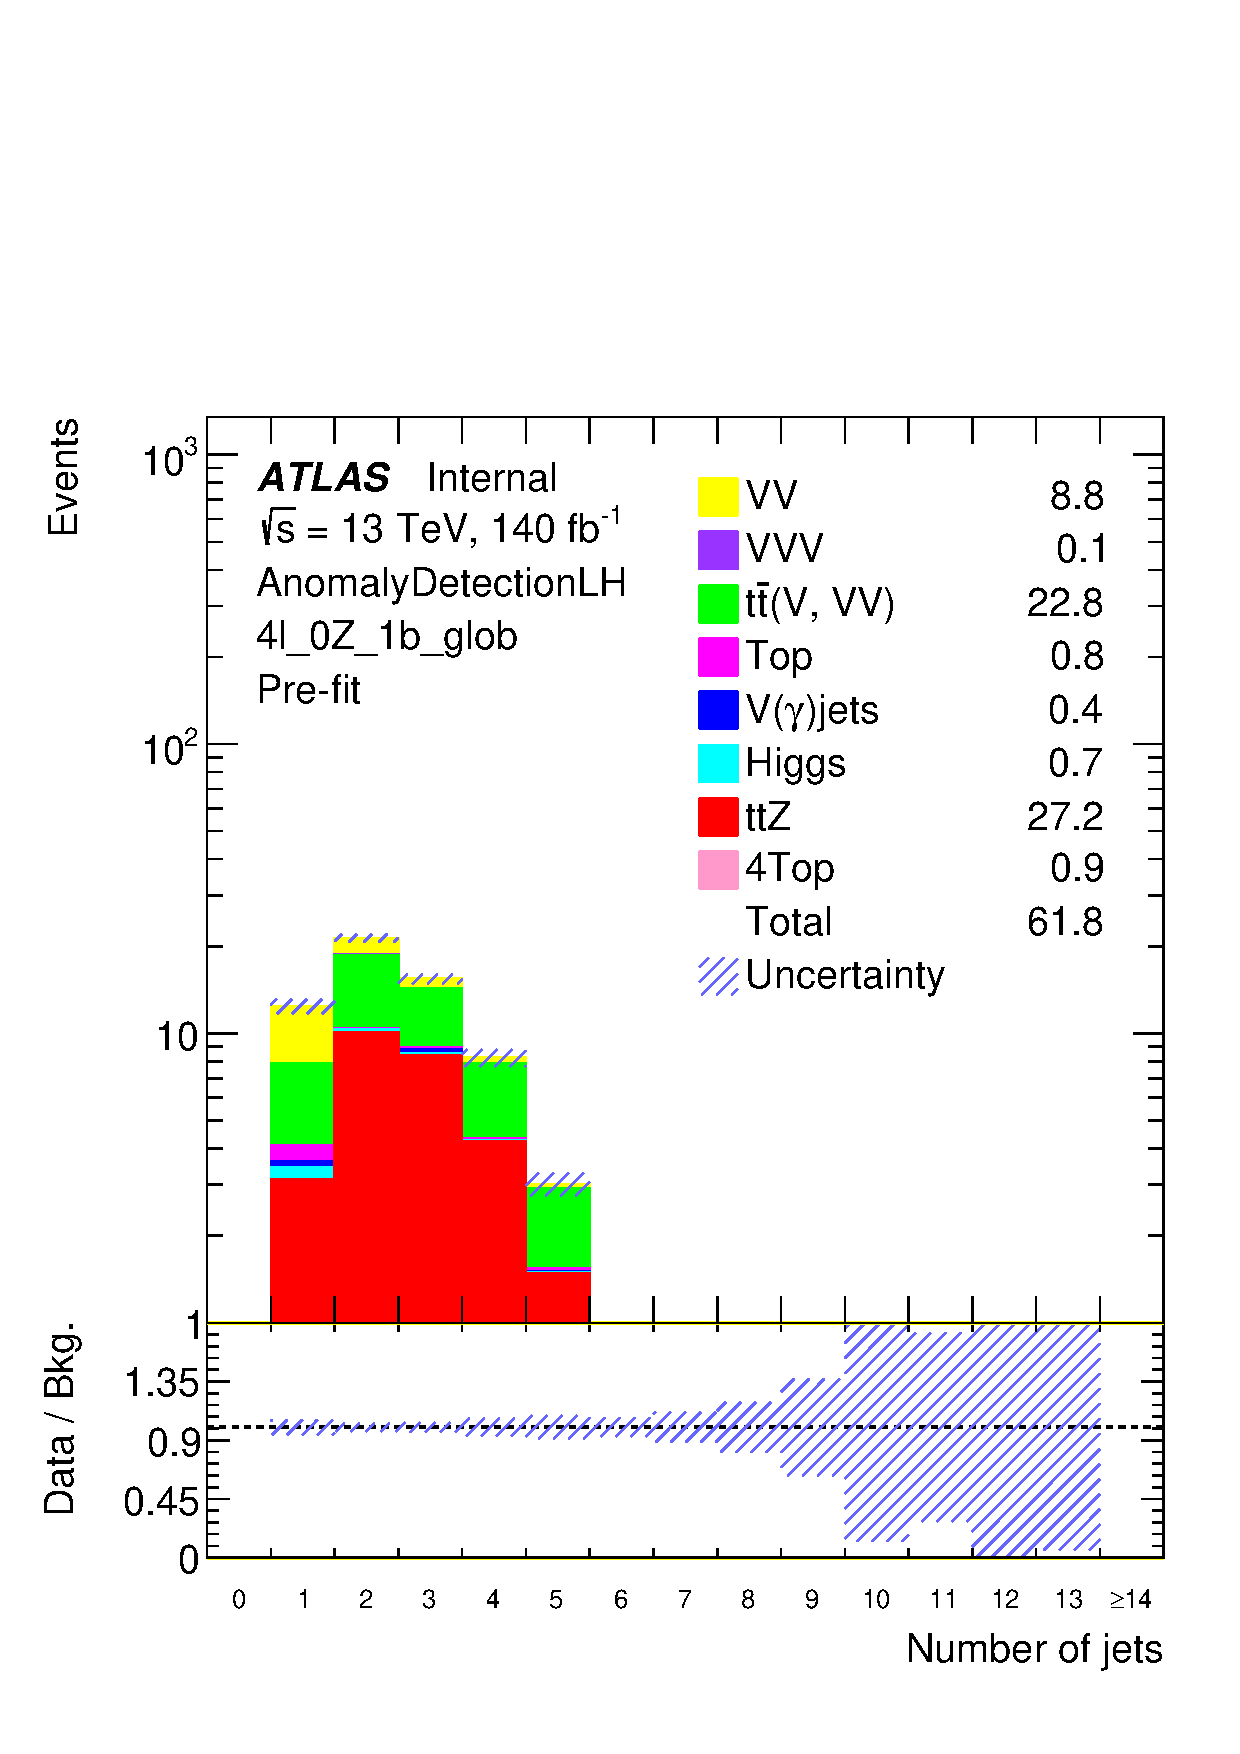
\includegraphics[width=0.24\textwidth]{plots/fourlepLH_run2/Plots/reg_4l_0Z_1b_glob_nJets.pdf} &
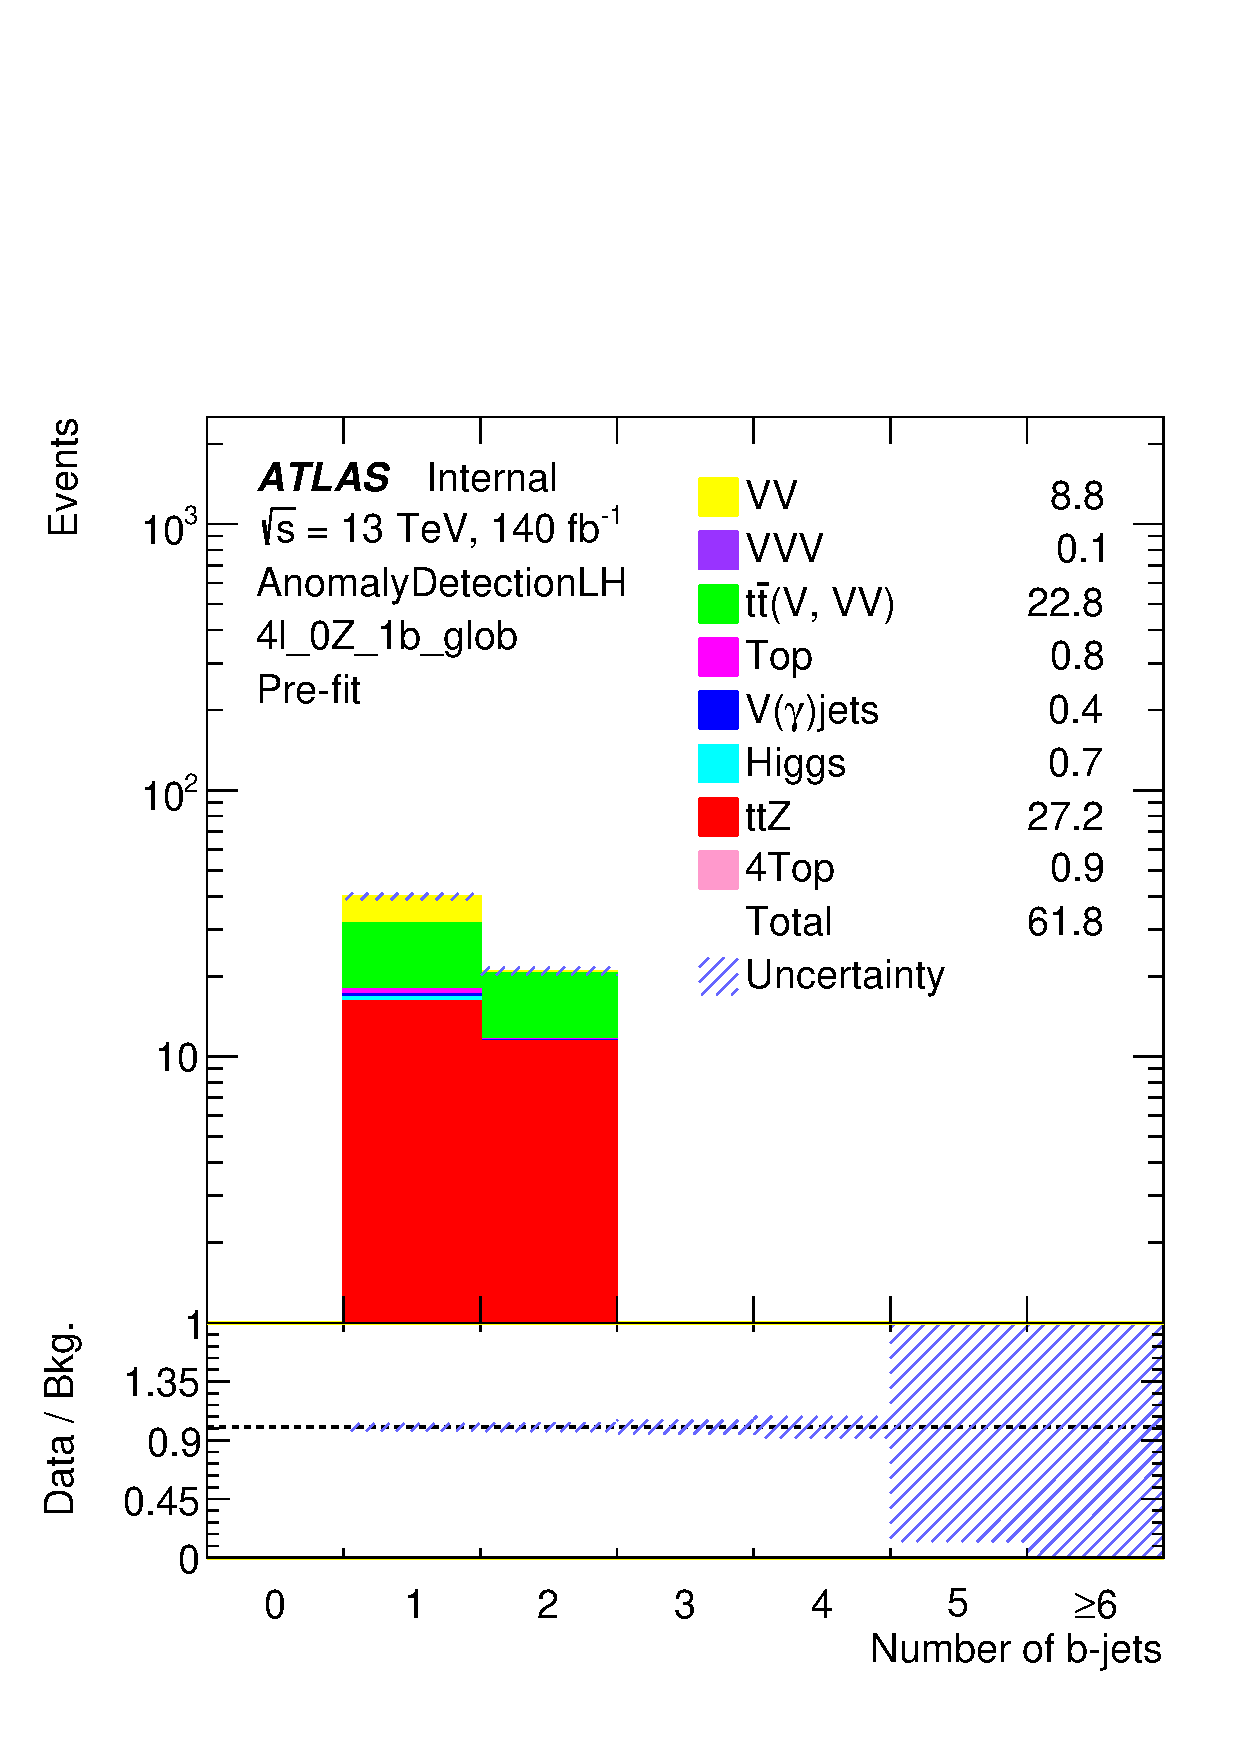
\includegraphics[width=0.24\textwidth]{plots/fourlepLH_run2/Plots/reg_4l_0Z_1b_glob_nbJets.pdf} &
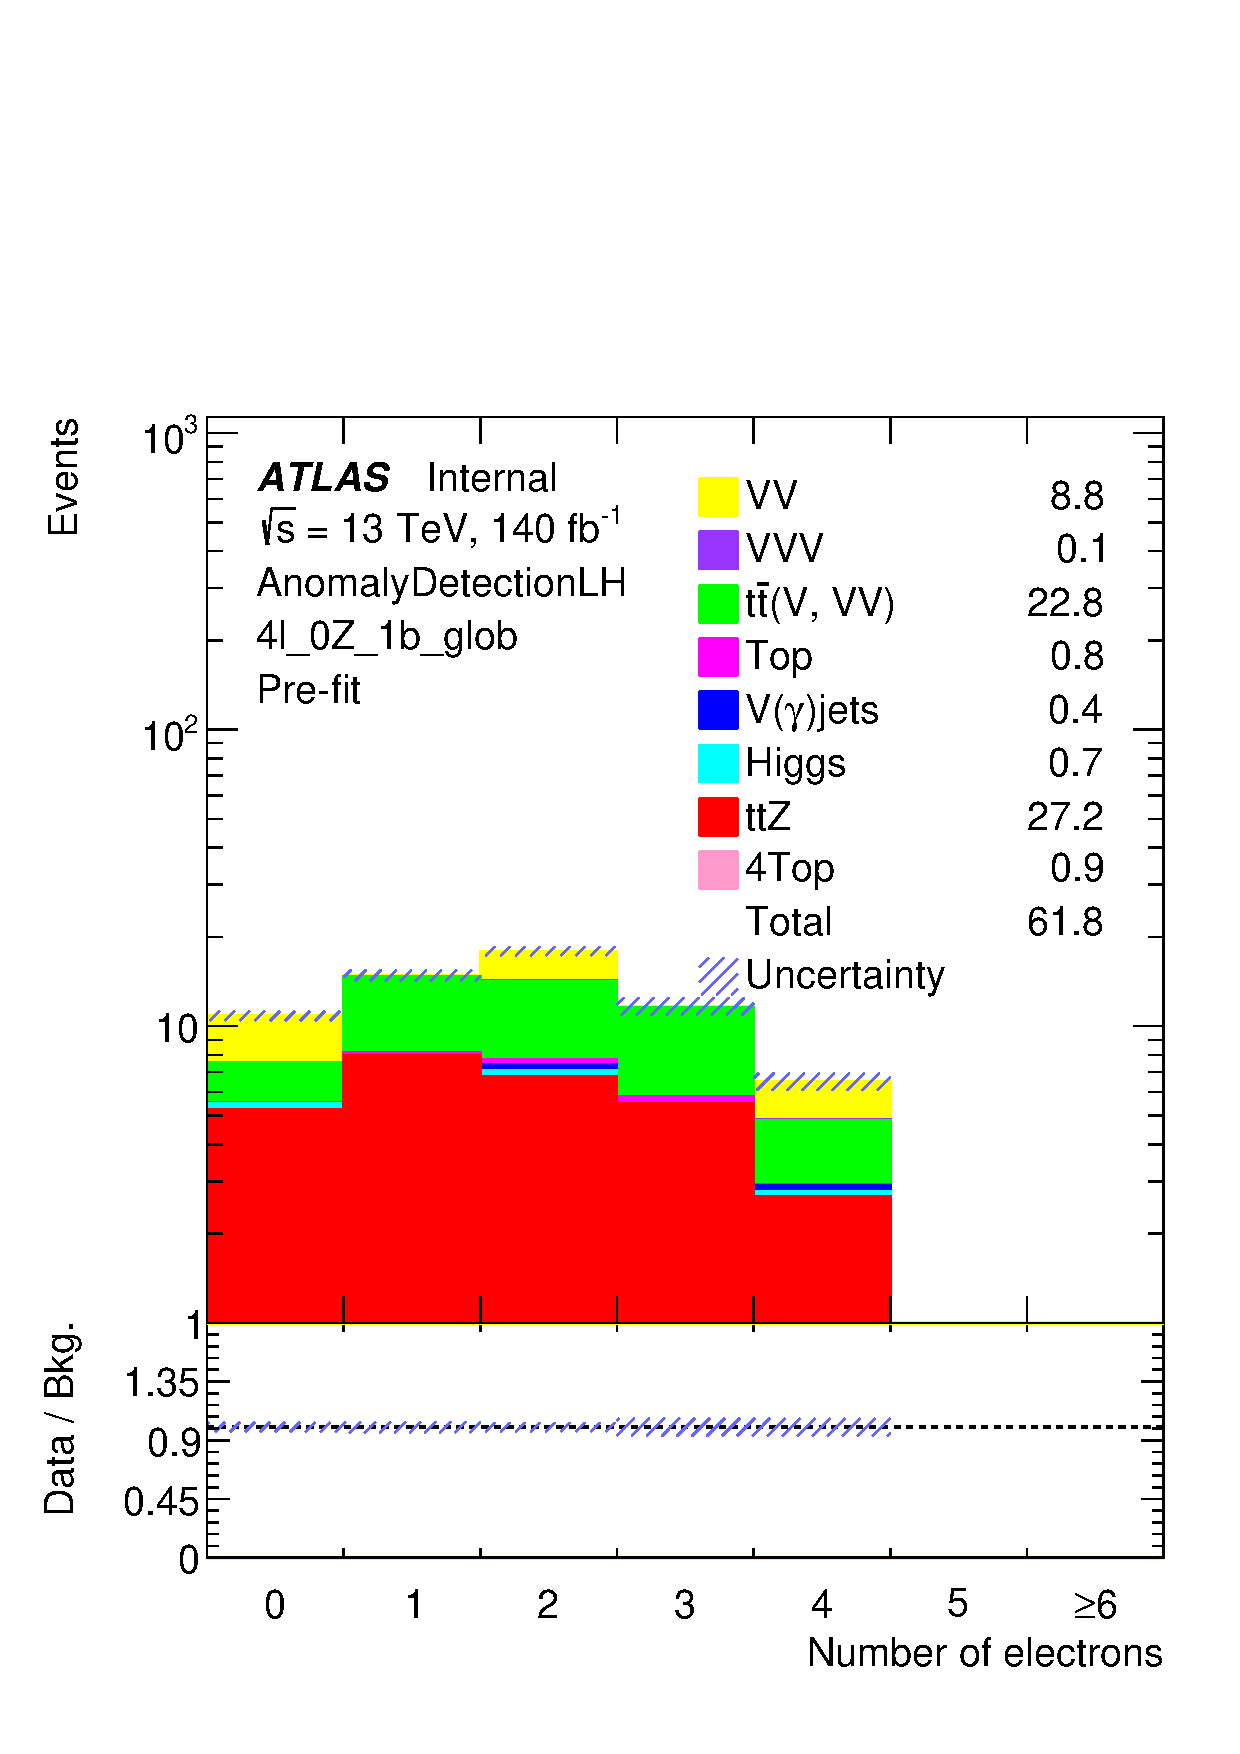
\includegraphics[width=0.24\textwidth]{plots/fourlepLH_run2/Plots/reg_4l_0Z_1b_glob_nElectrons.pdf} &
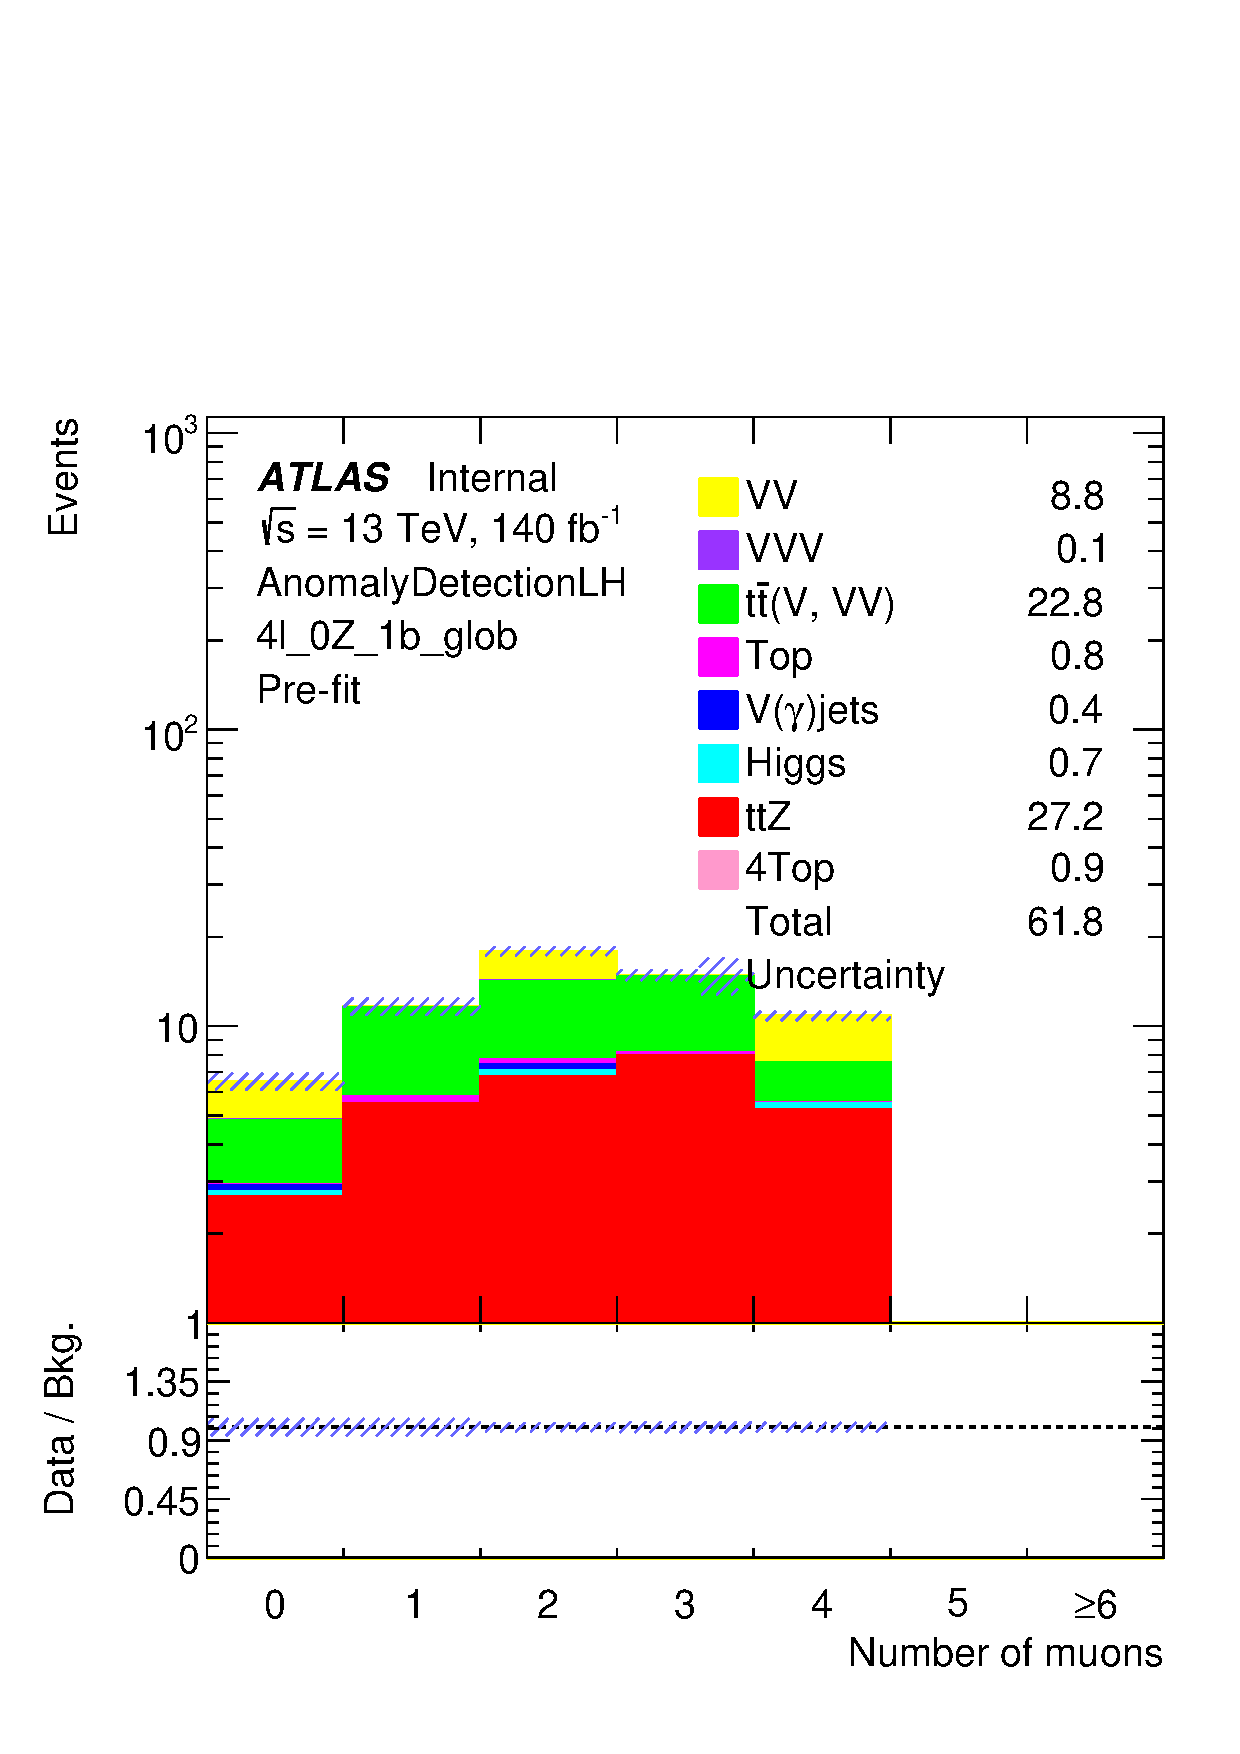
\includegraphics[width=0.24\textwidth]{plots/fourlepLH_run2/Plots/reg_4l_0Z_1b_glob_nMuons.pdf} \\

\end{tabular}
\end{frame}

\begin{frame}{\texttt{Results: 4l\_0Z\_1b}}
\begin{tabular}{cccccc}
\includegraphics[width=0.24\textwidth]{plots/fourlepLH_run2/Plots/reg_4l_0Z_1b_seq_lep_pt_0.pdf} &
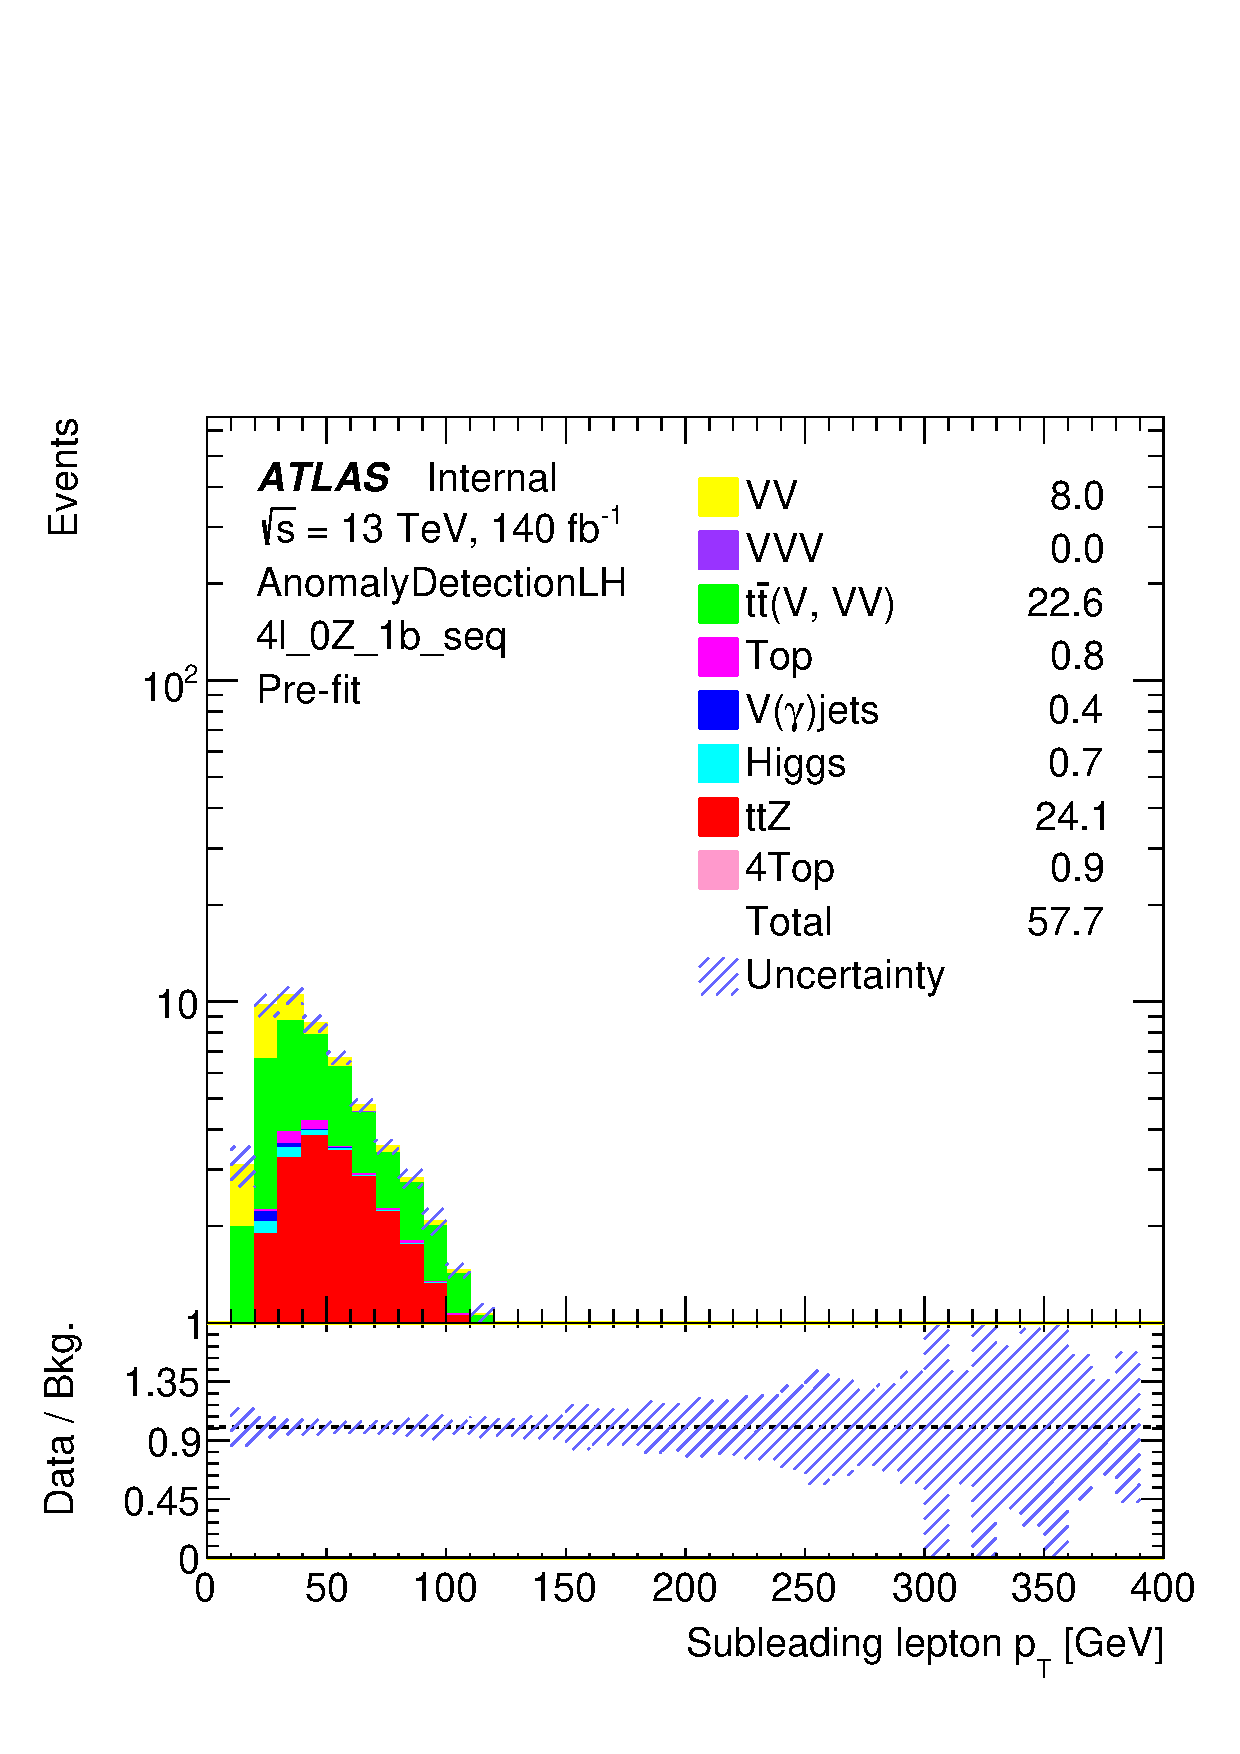
\includegraphics[width=0.24\textwidth]{plots/fourlepLH_run2/Plots/reg_4l_0Z_1b_seq_lep_pt_1.pdf} &
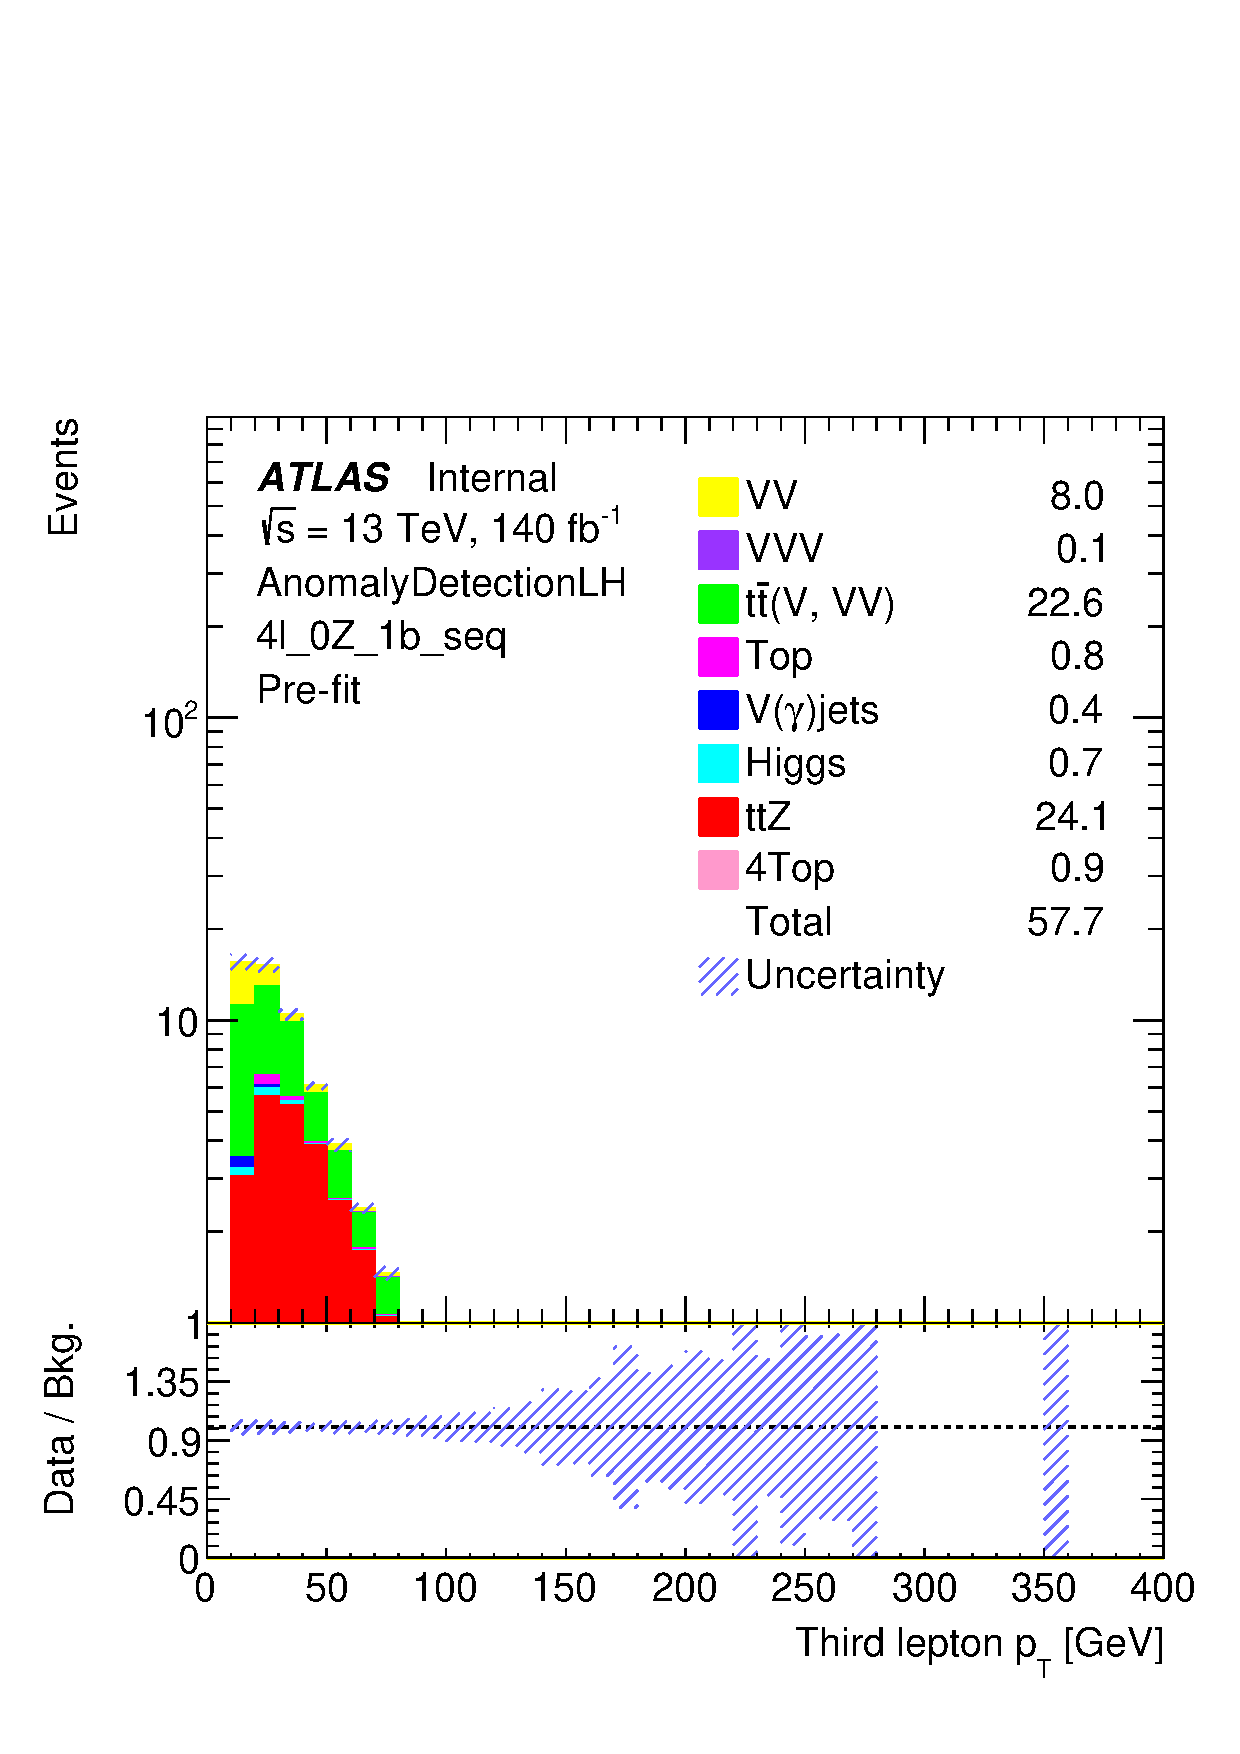
\includegraphics[width=0.24\textwidth]{plots/fourlepLH_run2/Plots/reg_4l_0Z_1b_seq_lep_pt_2.pdf} &
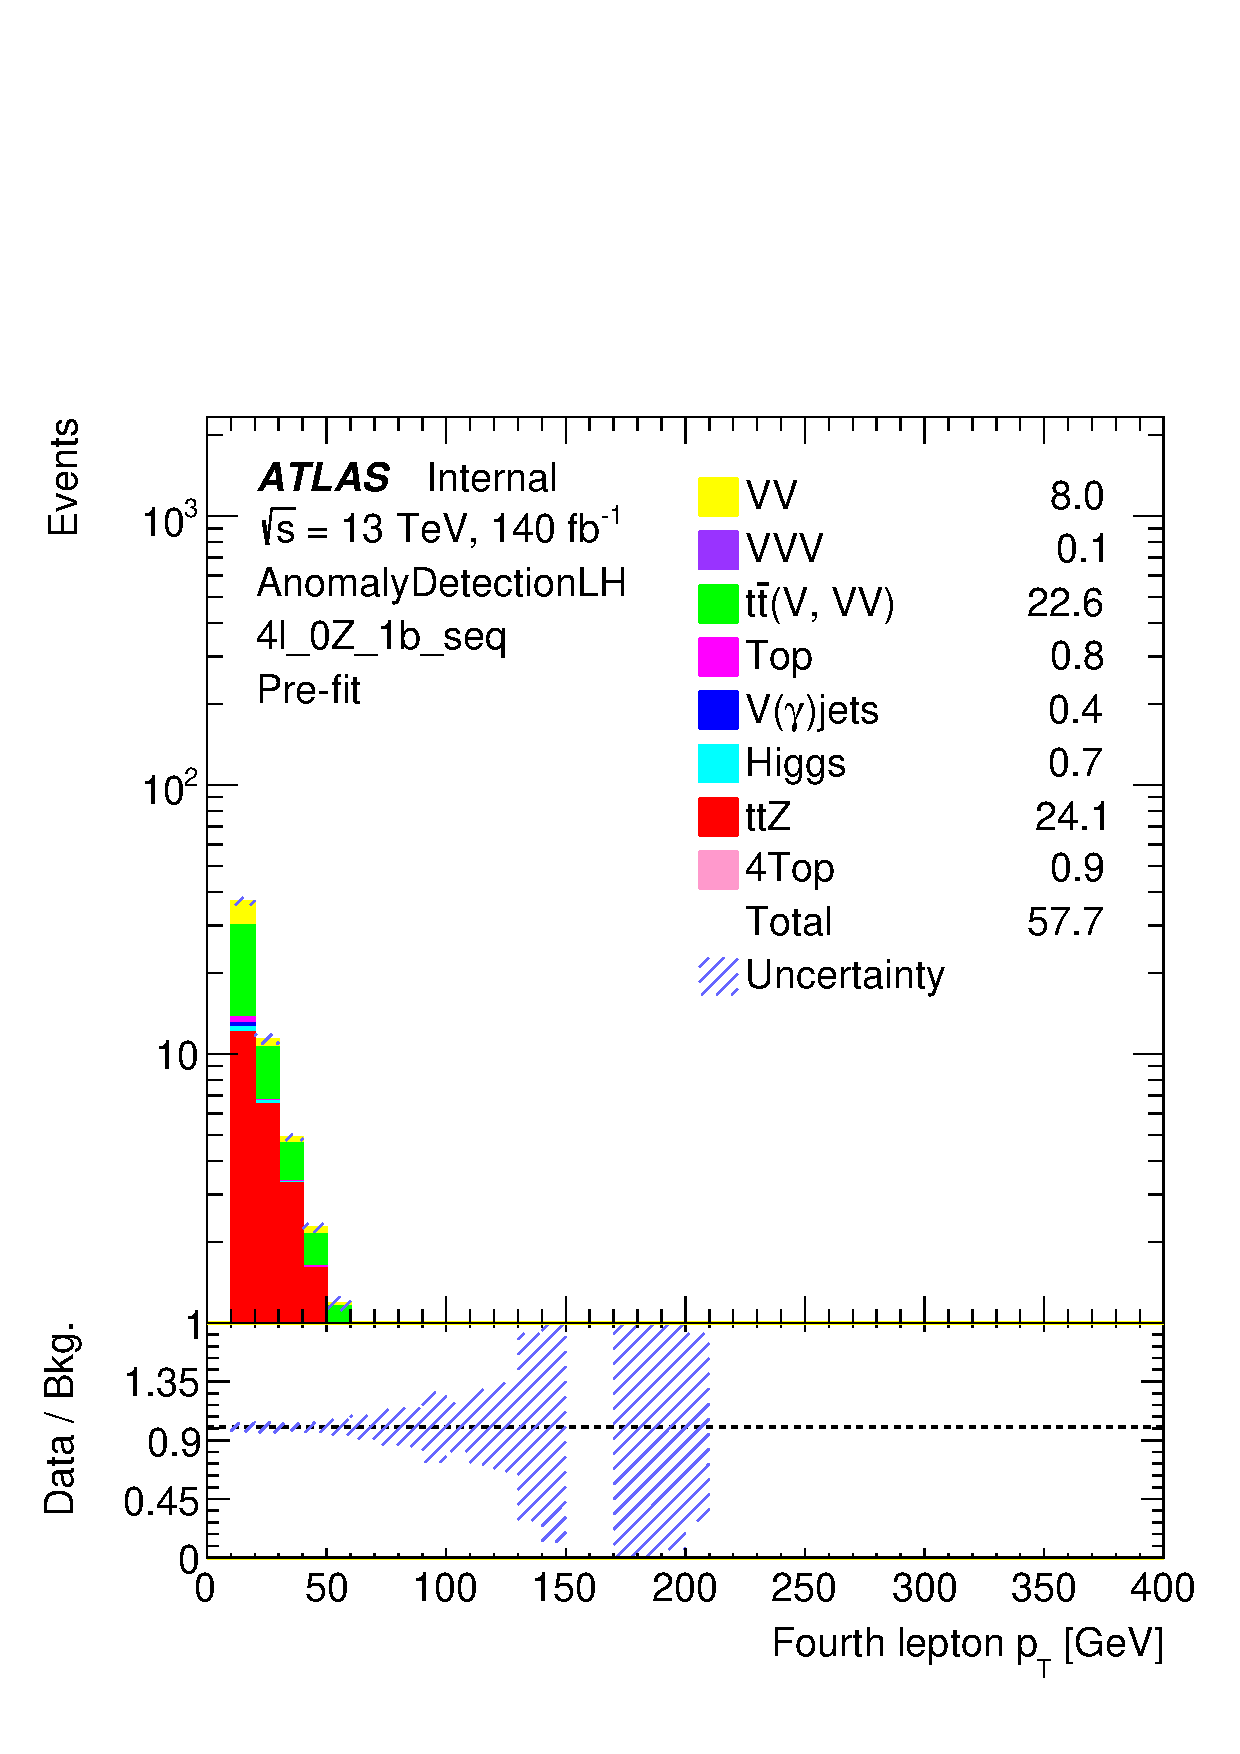
\includegraphics[width=0.24\textwidth]{plots/fourlepLH_run2/Plots/reg_4l_0Z_1b_seq_lep_pt_3.pdf} \\

\includegraphics[width=0.24\textwidth]{plots/fourlepLH_run2/Plots/reg_4l_0Z_1b_glob_lep_pt_0.pdf} &
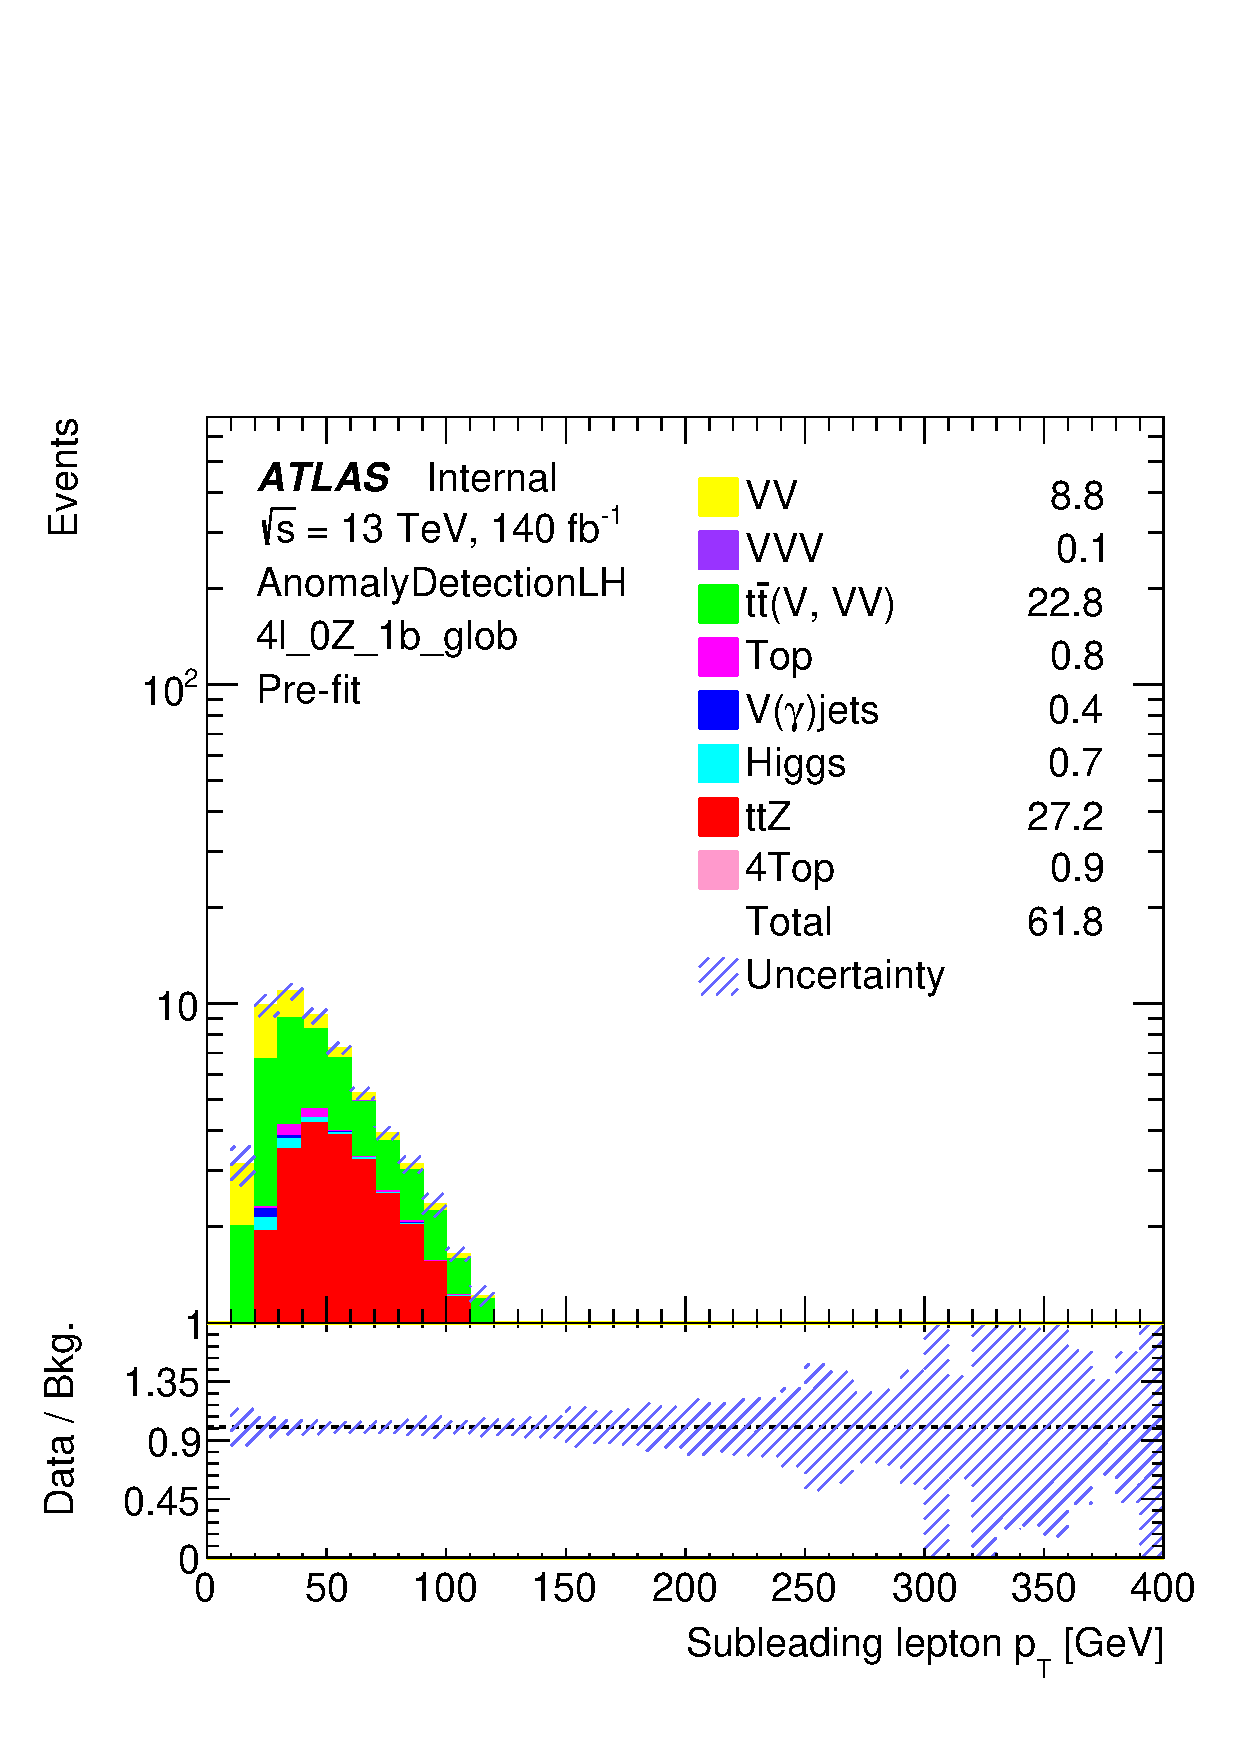
\includegraphics[width=0.24\textwidth]{plots/fourlepLH_run2/Plots/reg_4l_0Z_1b_glob_lep_pt_1.pdf} &
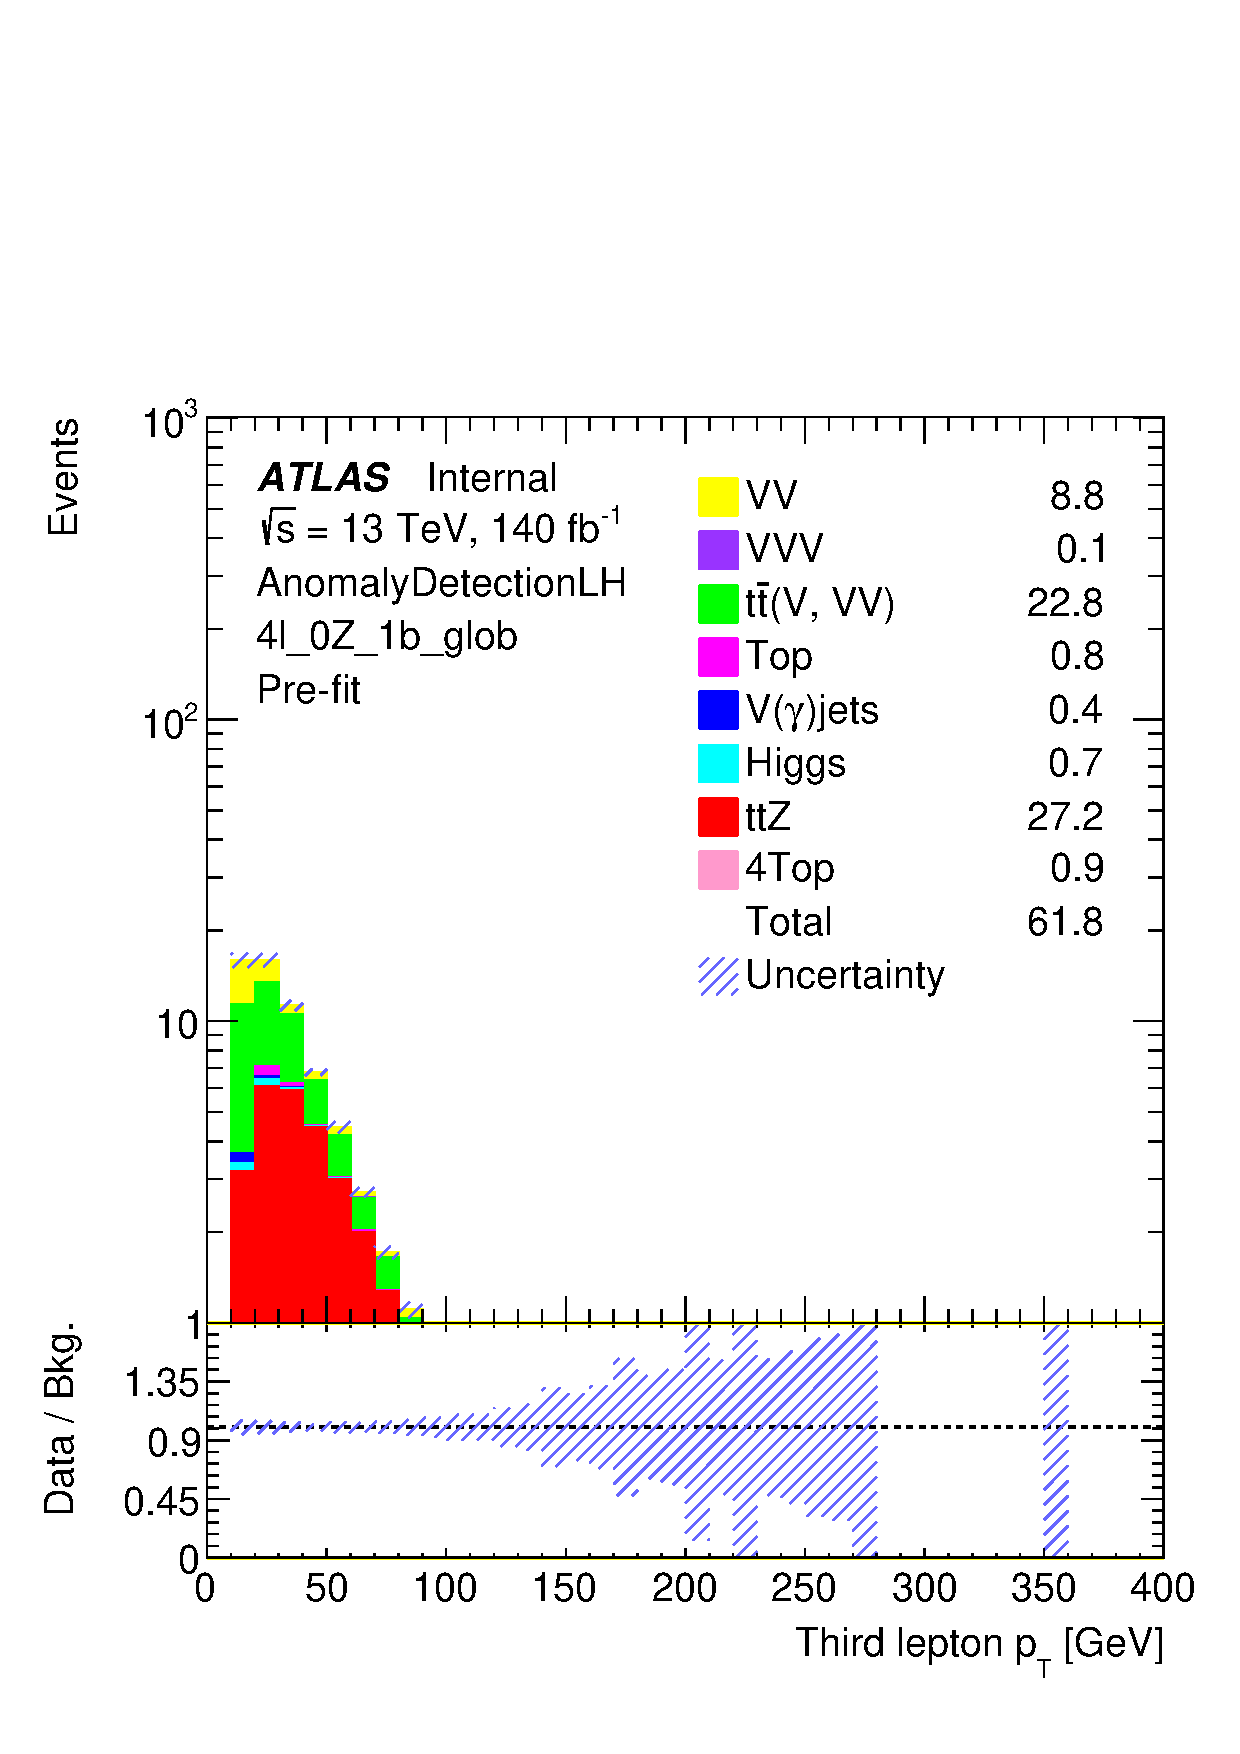
\includegraphics[width=0.24\textwidth]{plots/fourlepLH_run2/Plots/reg_4l_0Z_1b_glob_lep_pt_2.pdf} &
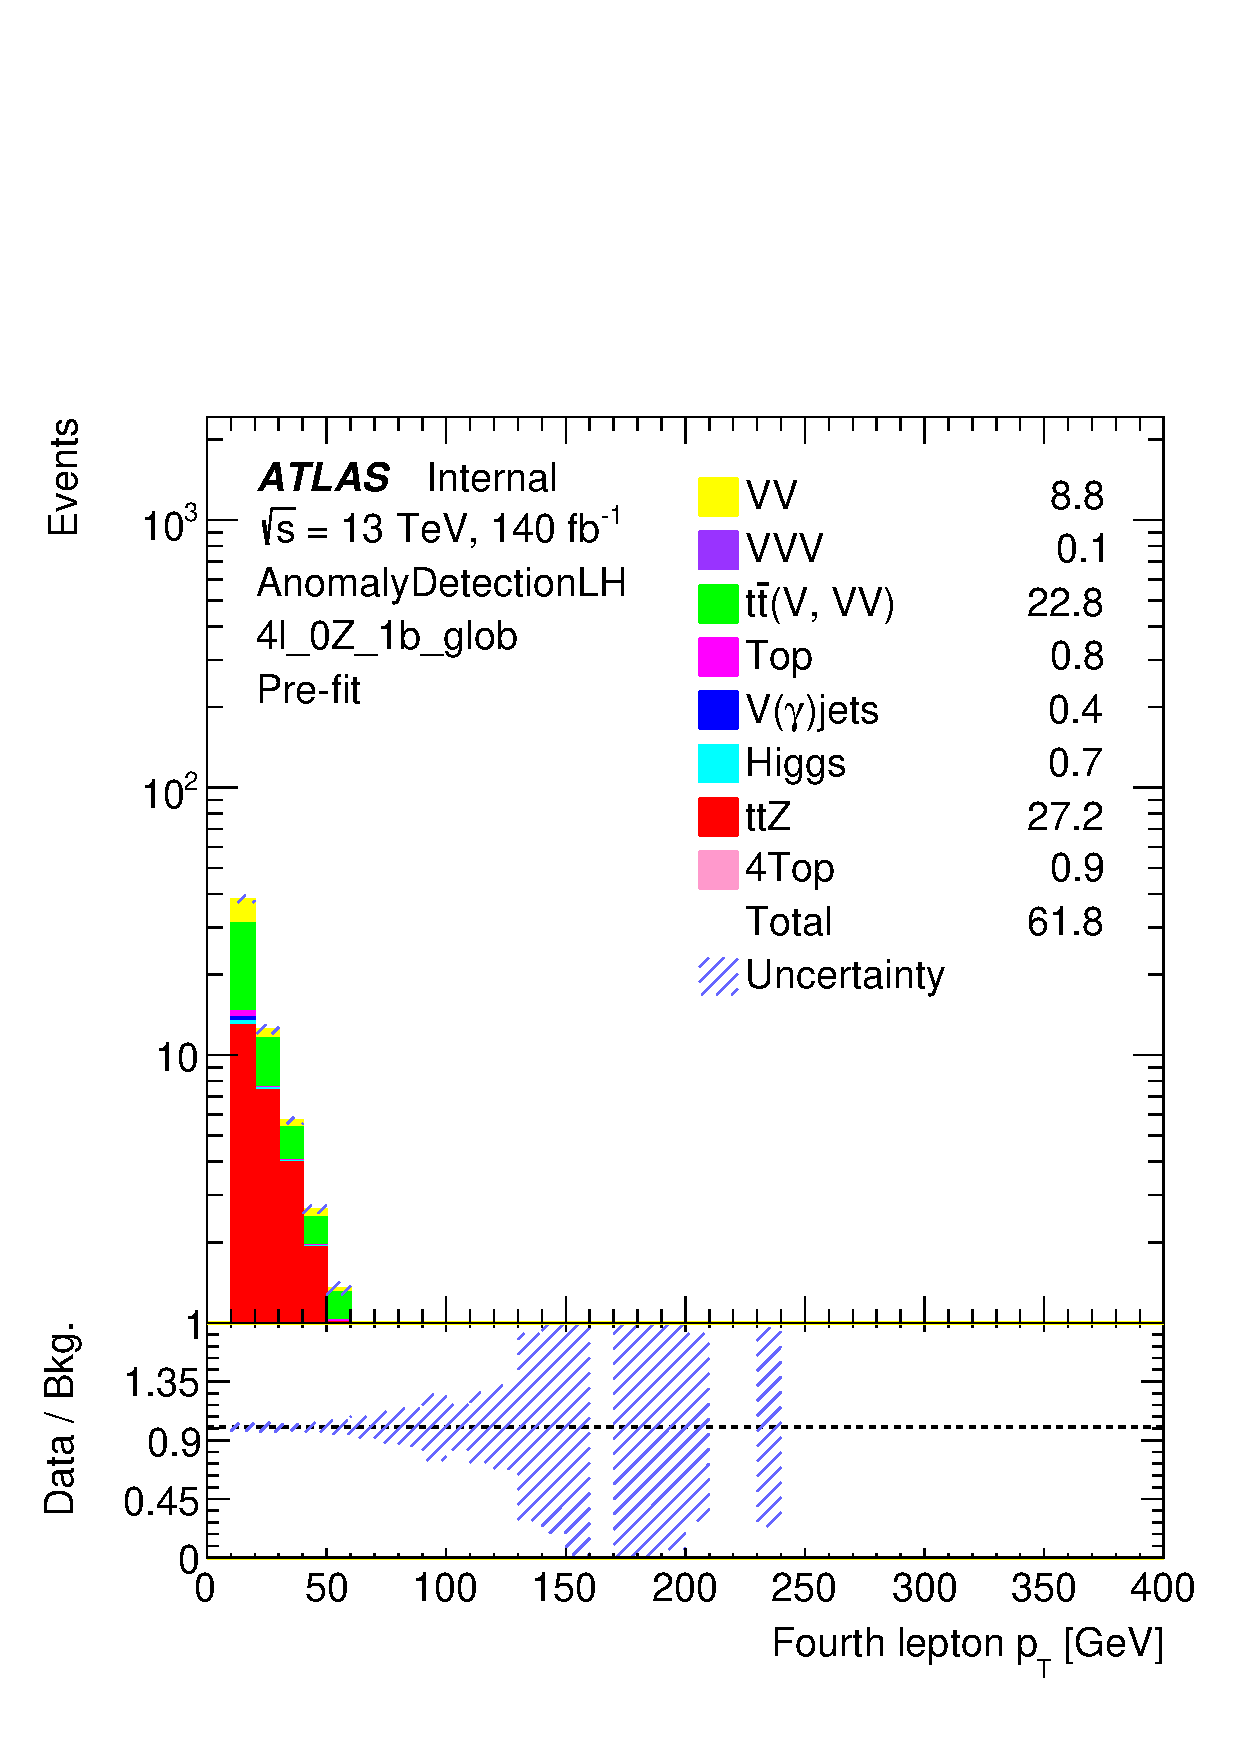
\includegraphics[width=0.24\textwidth]{plots/fourlepLH_run2/Plots/reg_4l_0Z_1b_glob_lep_pt_3.pdf} \\

\end{tabular}

\end{frame}
\subsection{4l\_1Z}
\begin{frame}{\texttt{Focused selection: 4l\_1Z}}
%\tiny
\centering
\begin{tabular}{|c|c|}
\hline

4l\_1Z\_seq &
4l\_1Z\_glob \\
\hline
\multicolumn{2}{|c|}{\texttt{globalTriggerMatchSLTorDLT\_LooseLH\_custTrig\_NOSYS}} \\
\multicolumn{2}{|c|}{\texttt{pass\_fourlep\_LooseLH\_NOSYS} }\\
\multicolumn{2}{|c|}{\texttt{$N_{leptons}$=4}} \\
\multicolumn{2}{|c|}{\texttt{$N_{taus}$ $\geq 0$} } \\
\multicolumn{2}{|c|}{$N_{b\mathrm{-jets}}$ $\geq 0$} \\
\multicolumn{2}{|c|}{\texttt{Q = 0}} \\

\hline

\texttt{$|m_{Z1}^{seq}-91.2e3| < 10e3$} &
\texttt{$|m_{Z1}^{glob}-91.2e3| < 10e3$} &\\
\texttt{$|m_{Z2}^{seq}-91.2e3| < 10e3$} &
\texttt{$|m_{Z2}^{glob}-91.2e3| < 10e3$}\\

\hline

\end{tabular}
\end{frame}

\begin{frame}{\texttt{Results: 4l\_1Z}}
\centering
\begin{tabular}{cccccc}

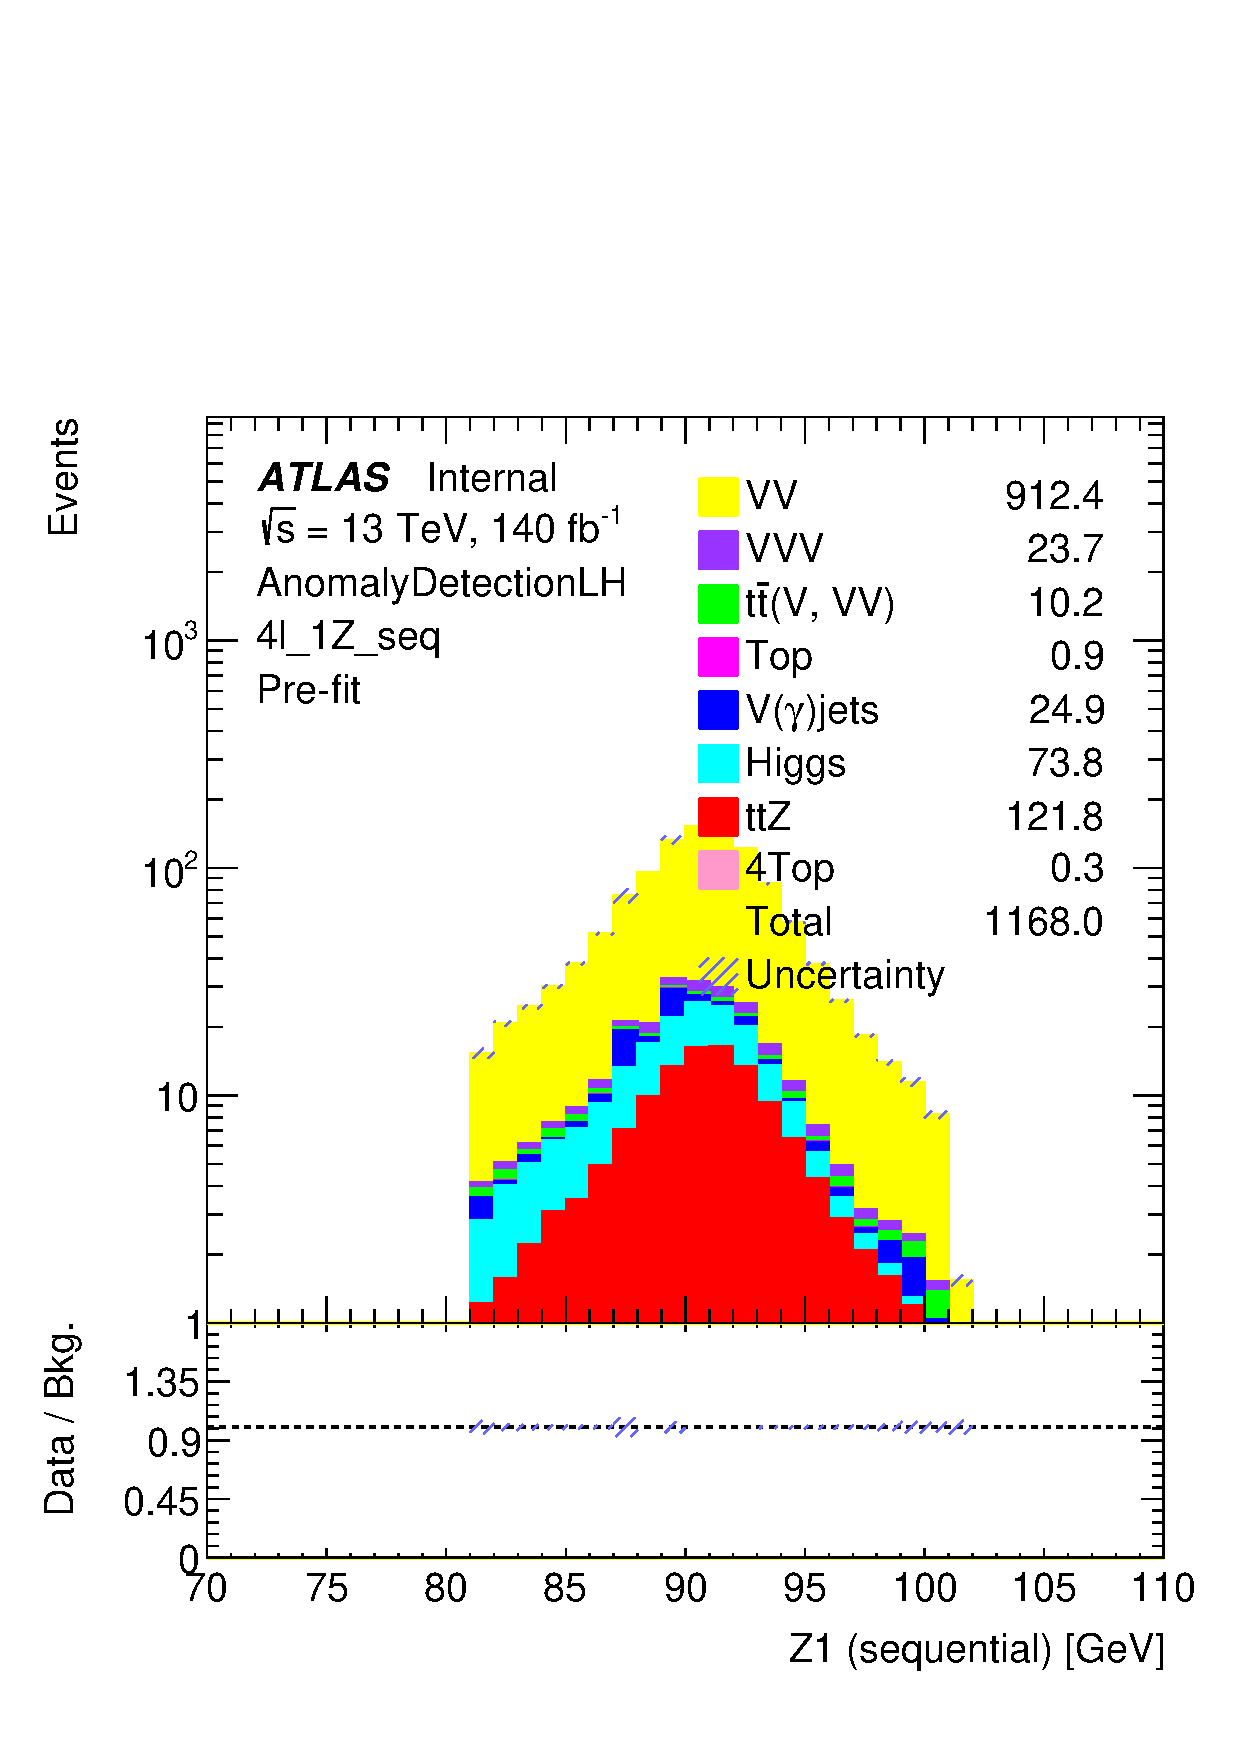
\includegraphics[width=0.24\textwidth]{plots/fourlepLH_run2/Plots/reg_4l_1Z_seq_Z1_mass_seq_1GeV.pdf} &
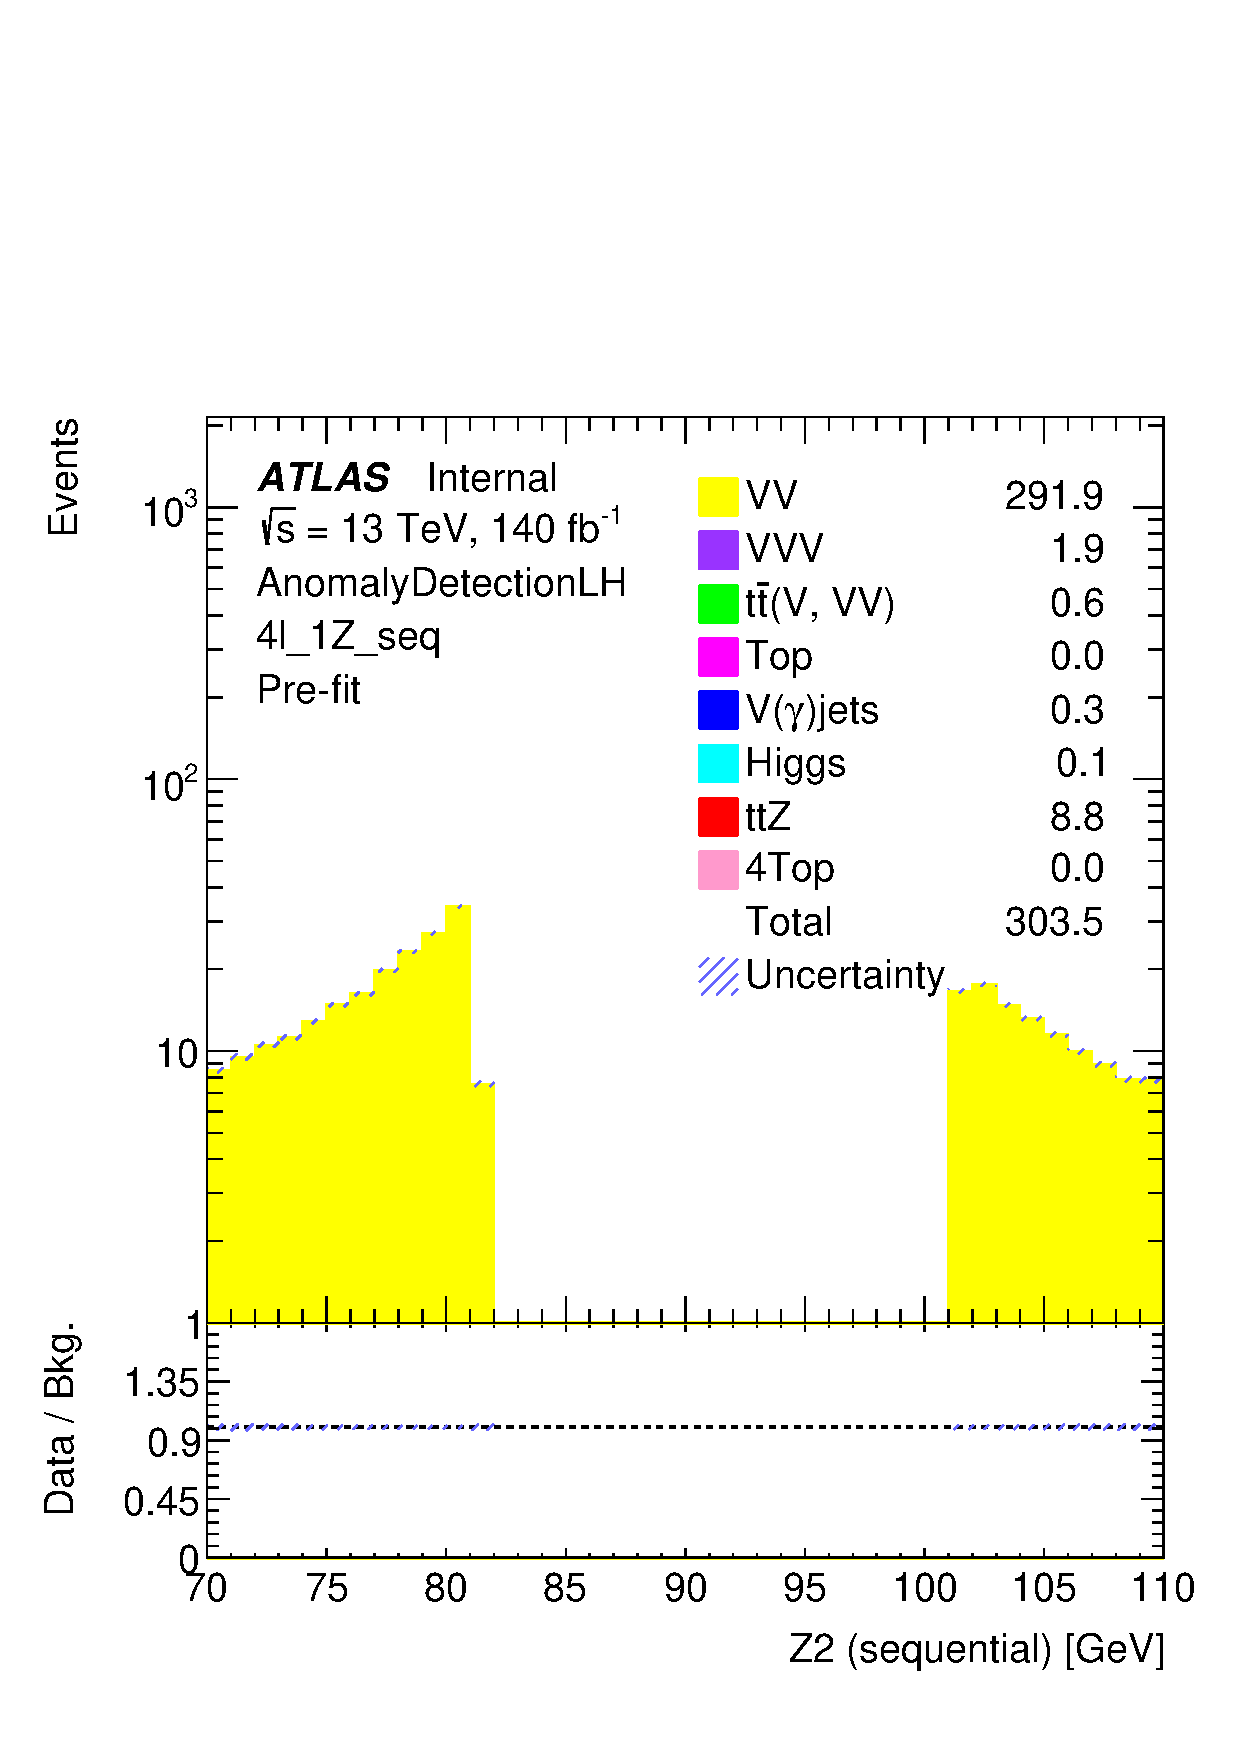
\includegraphics[width=0.24\textwidth]{plots/fourlepLH_run2/Plots/reg_4l_1Z_seq_Z2_mass_seq_1GeV.pdf}  &

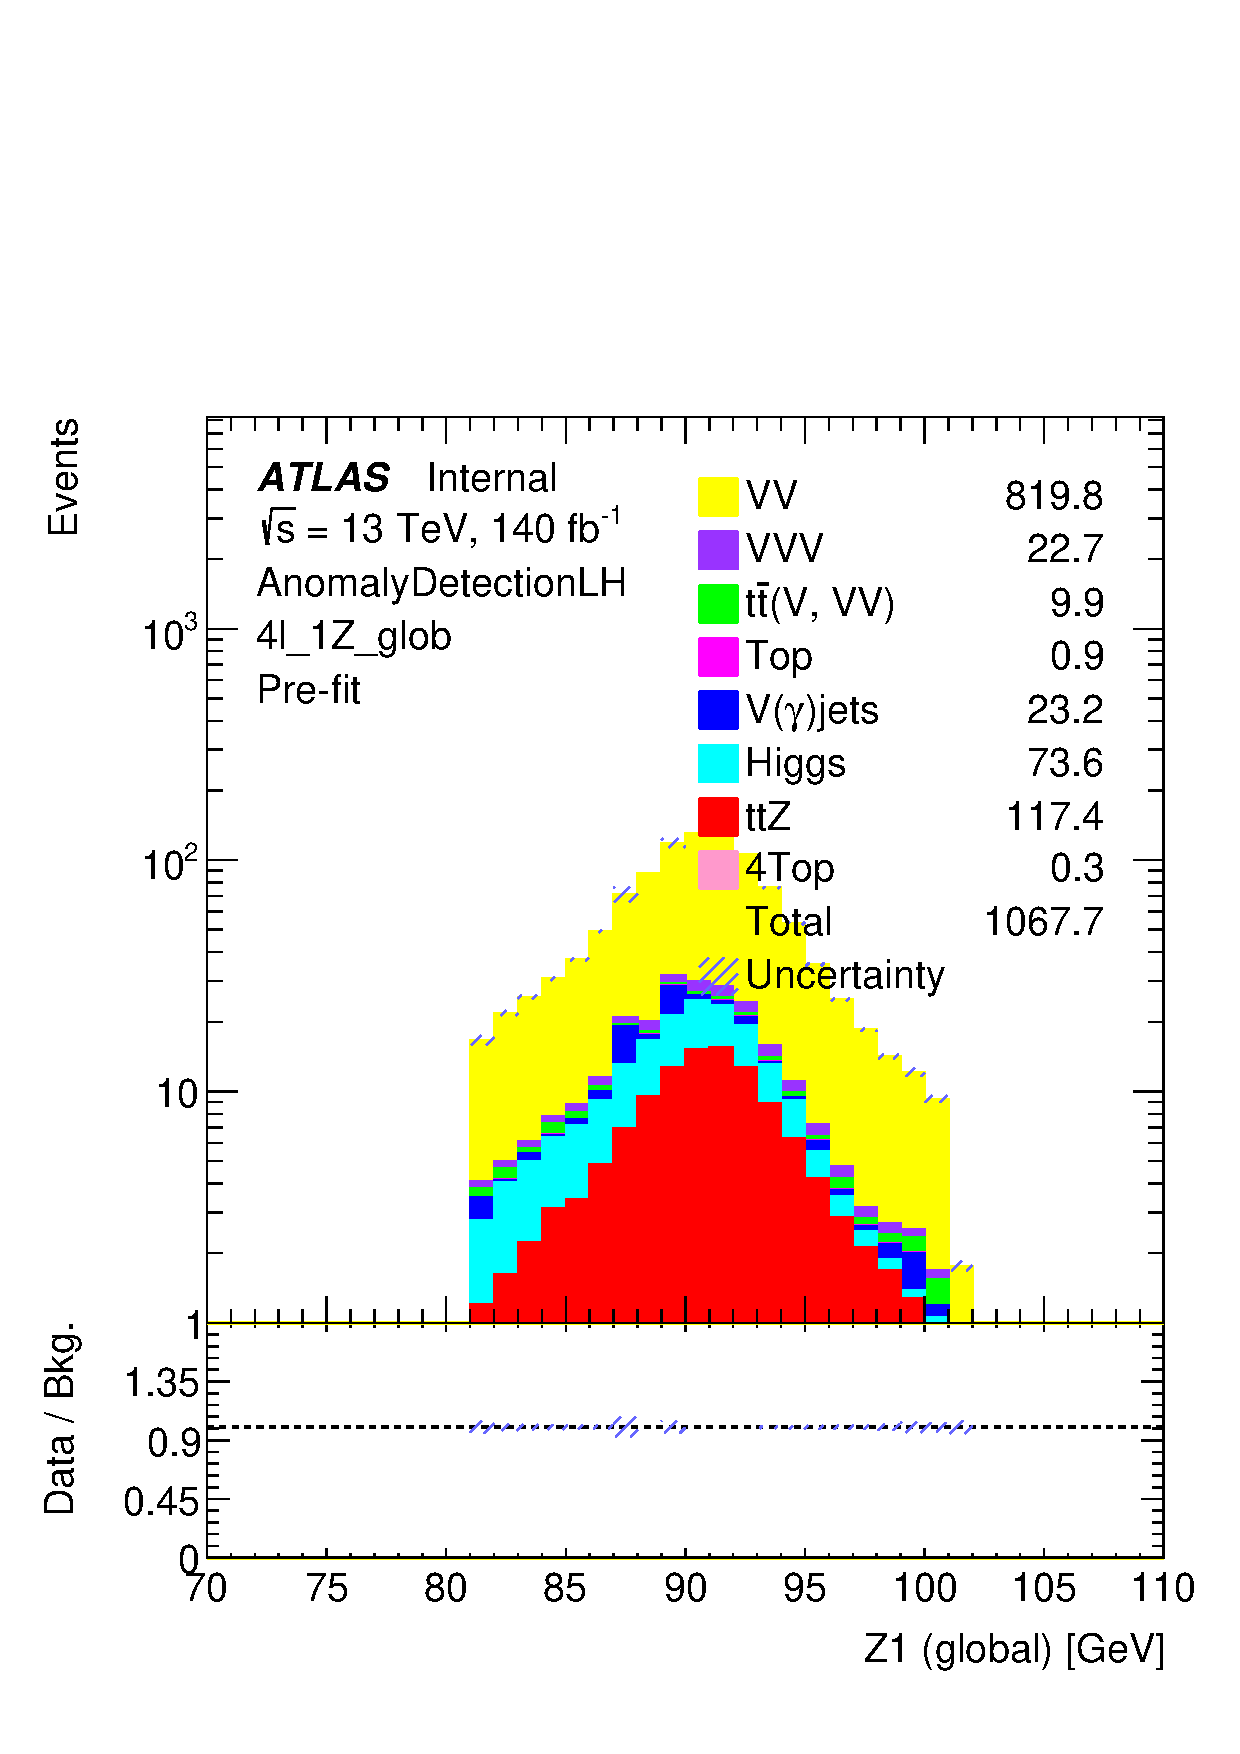
\includegraphics[width=0.24\textwidth]{plots/fourlepLH_run2/Plots/reg_4l_1Z_glob_Z1_mass_glob_1GeV.pdf} &
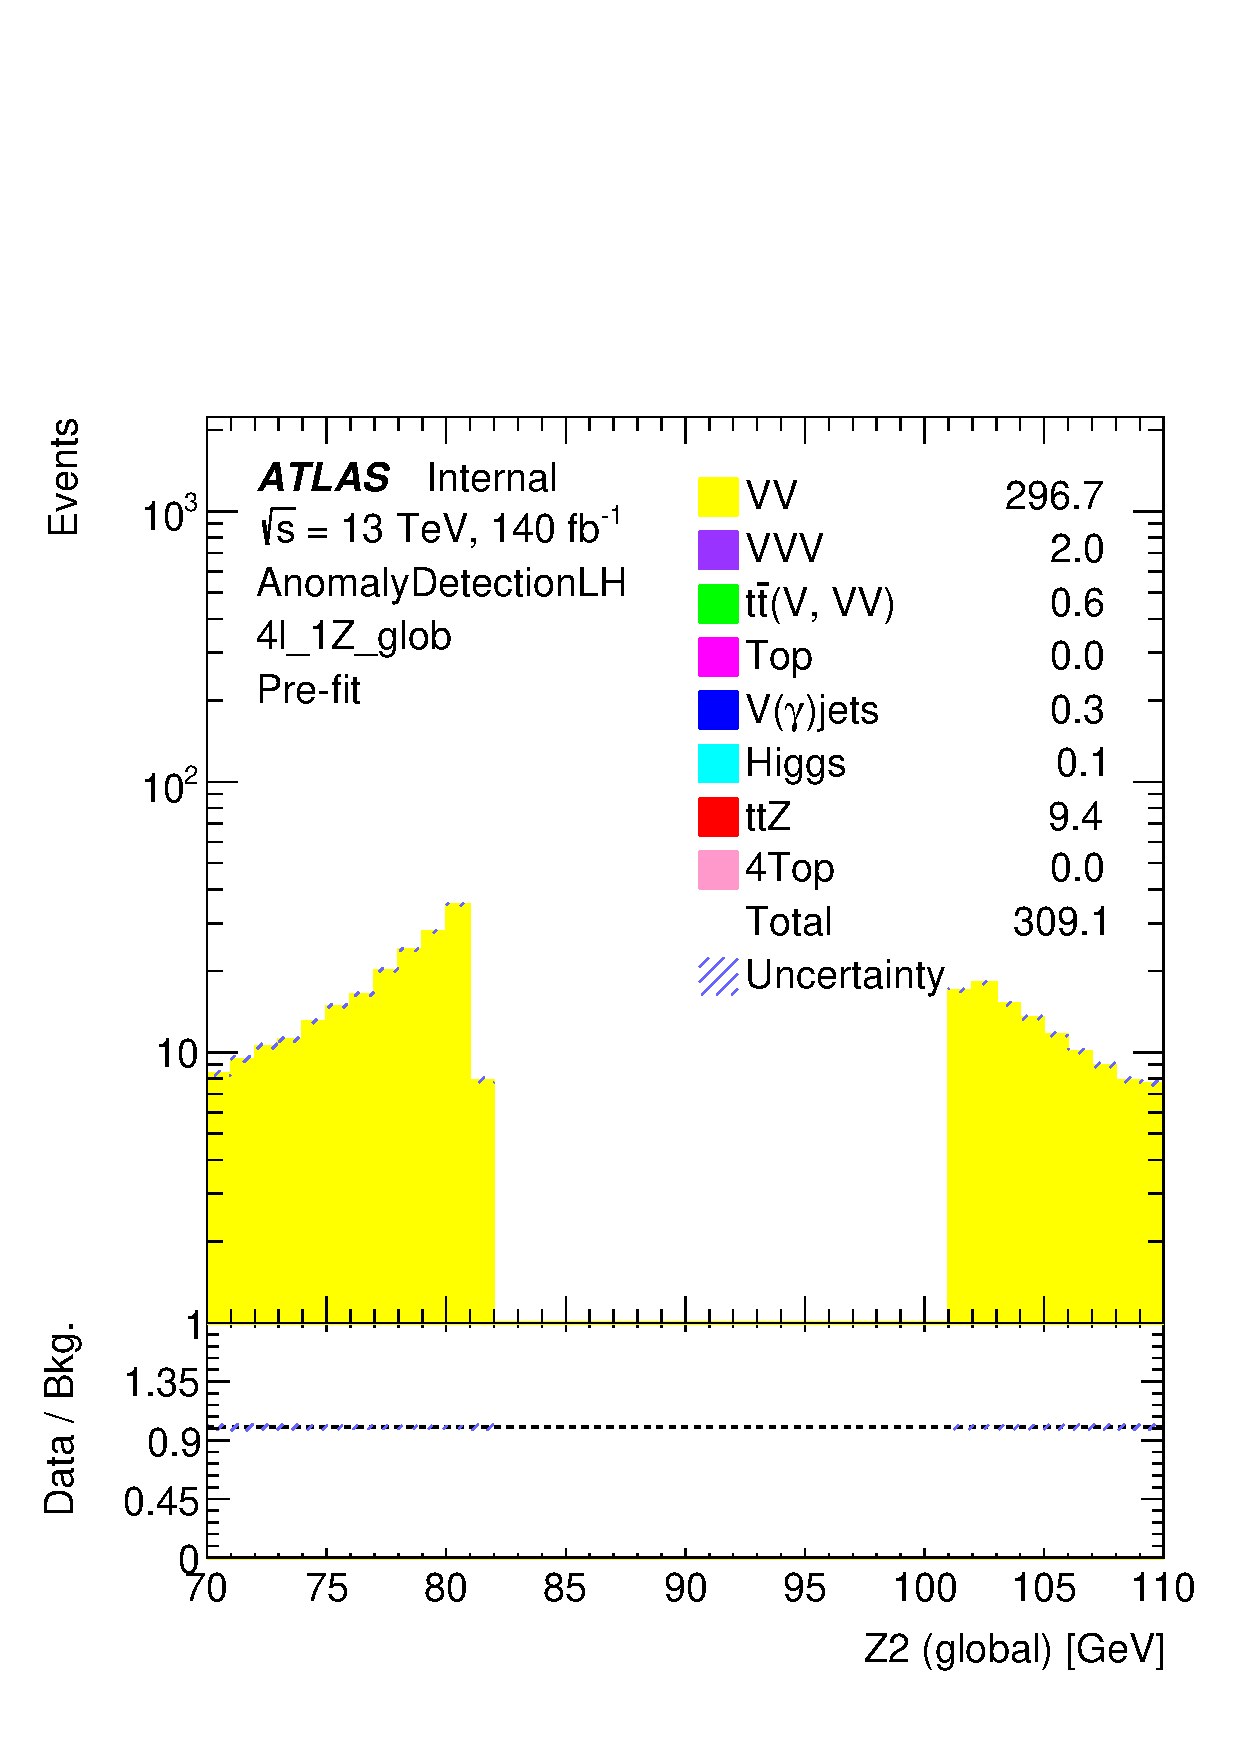
\includegraphics[width=0.24\textwidth]{plots/fourlepLH_run2/Plots/reg_4l_1Z_glob_Z2_mass_glob_1GeV.pdf}\\

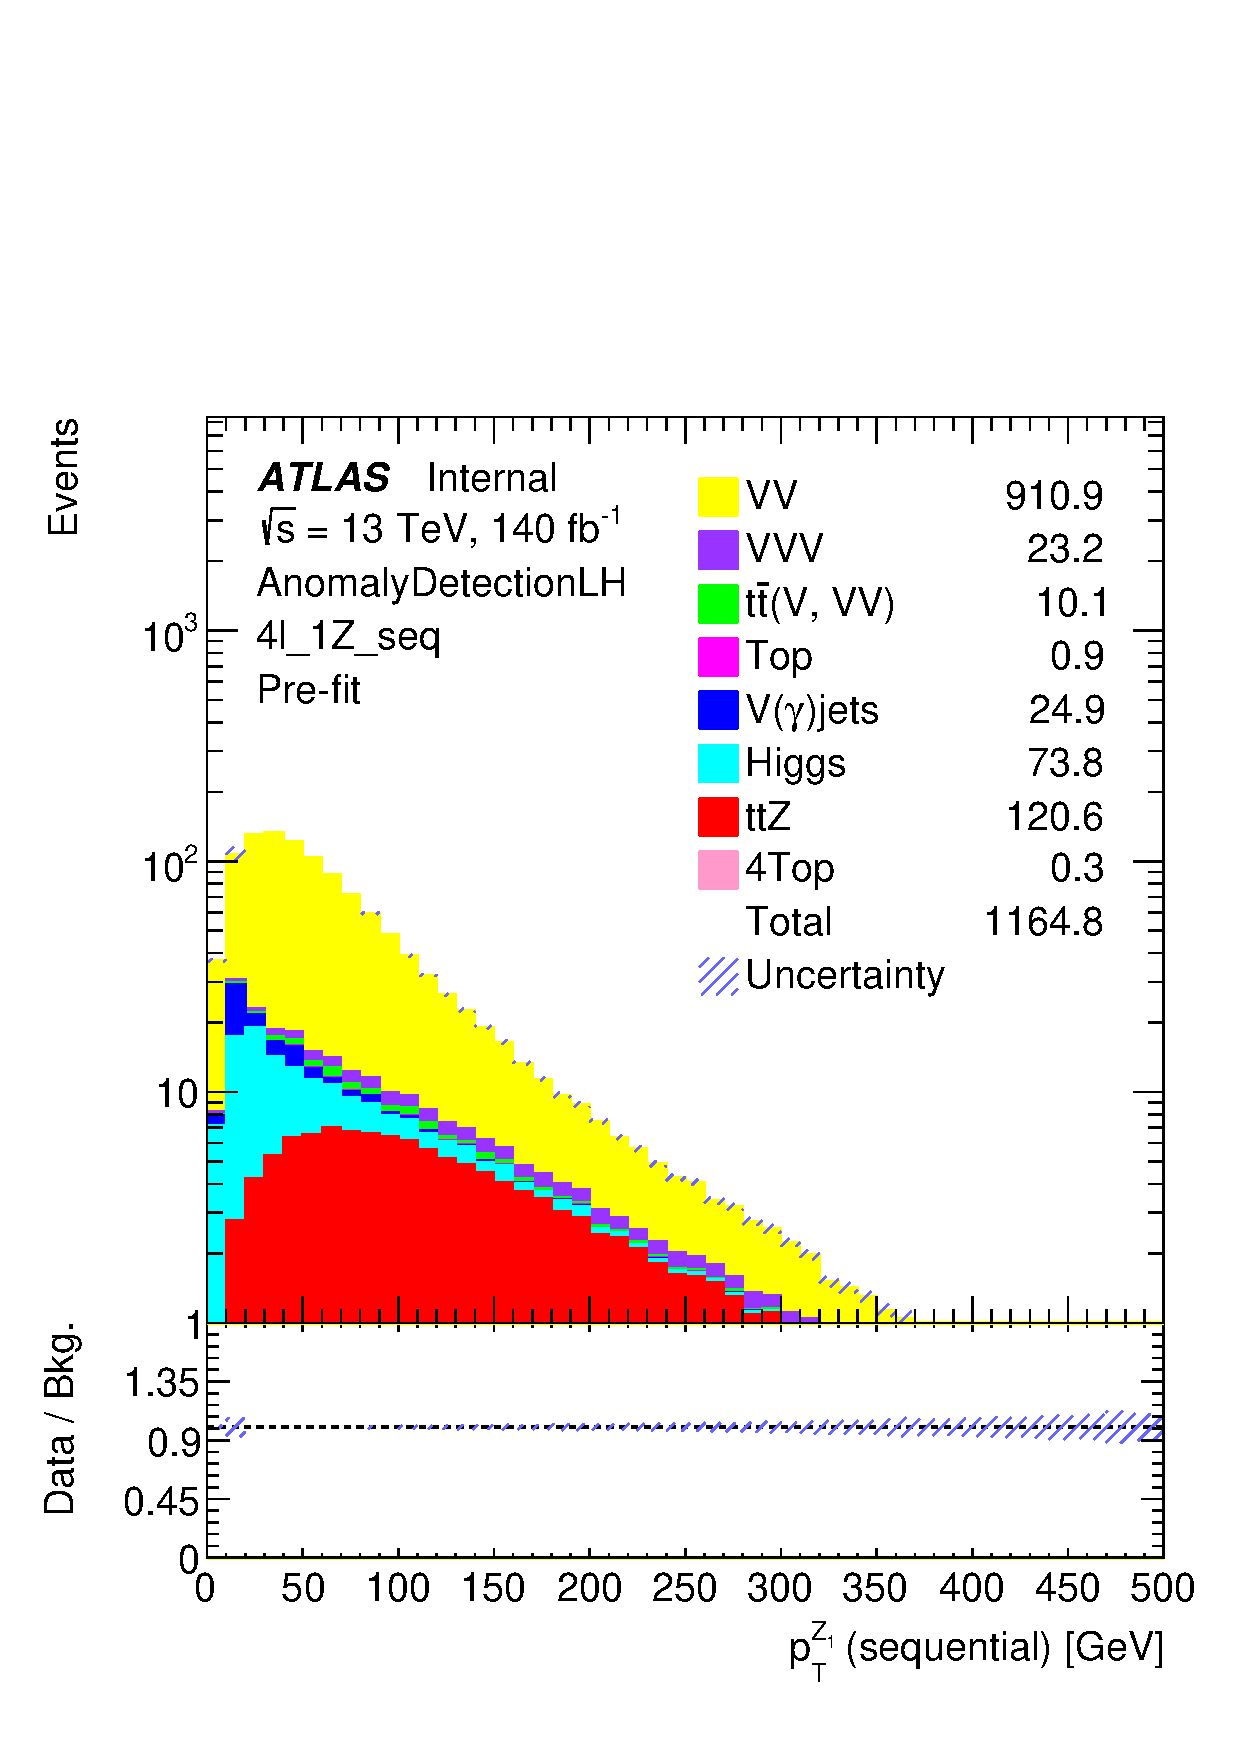
\includegraphics[width=0.24\textwidth]{plots/fourlepLH_run2/Plots/reg_4l_1Z_seq_Z1_pt_seq.pdf} &
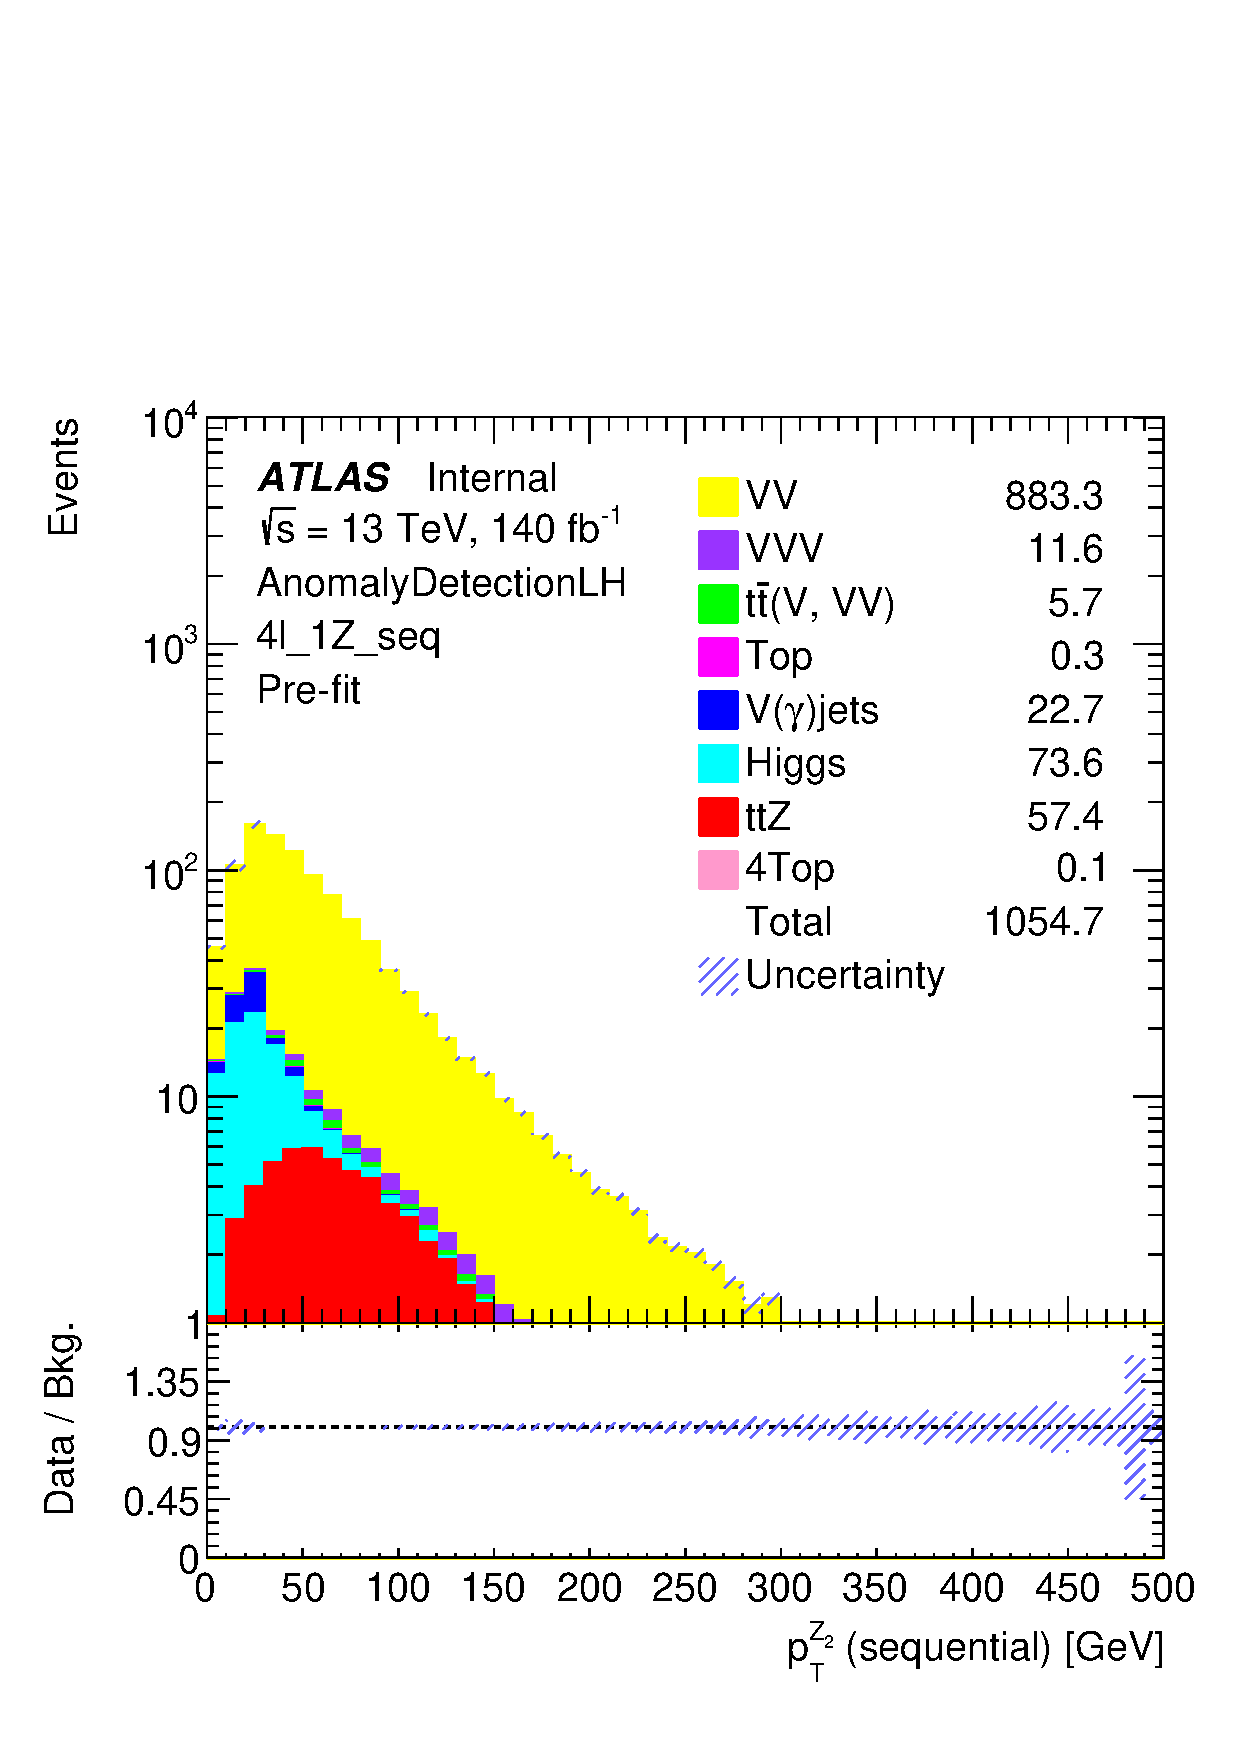
\includegraphics[width=0.24\textwidth]{plots/fourlepLH_run2/Plots/reg_4l_1Z_seq_Z2_pt_seq.pdf}  &

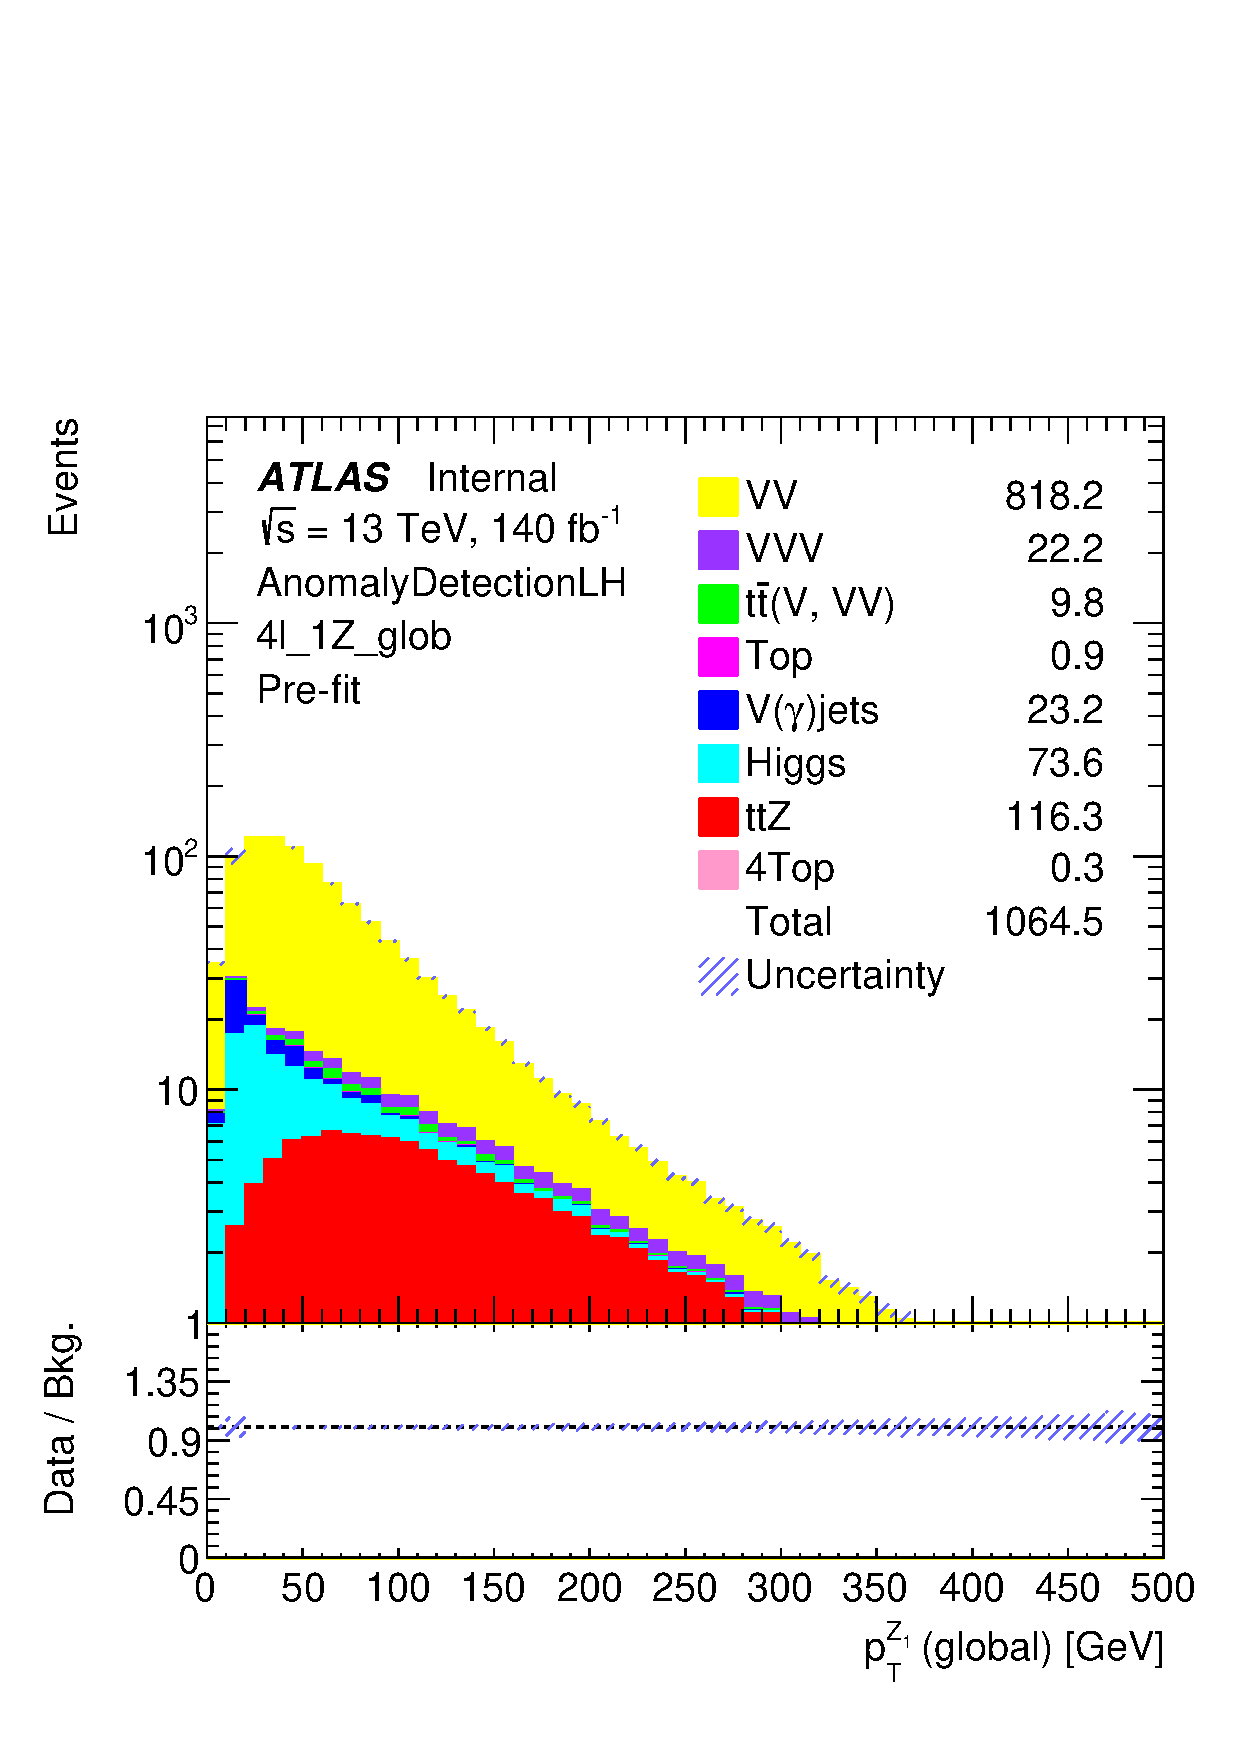
\includegraphics[width=0.24\textwidth]{plots/fourlepLH_run2/Plots/reg_4l_1Z_glob_Z1_pt_glob.pdf} &
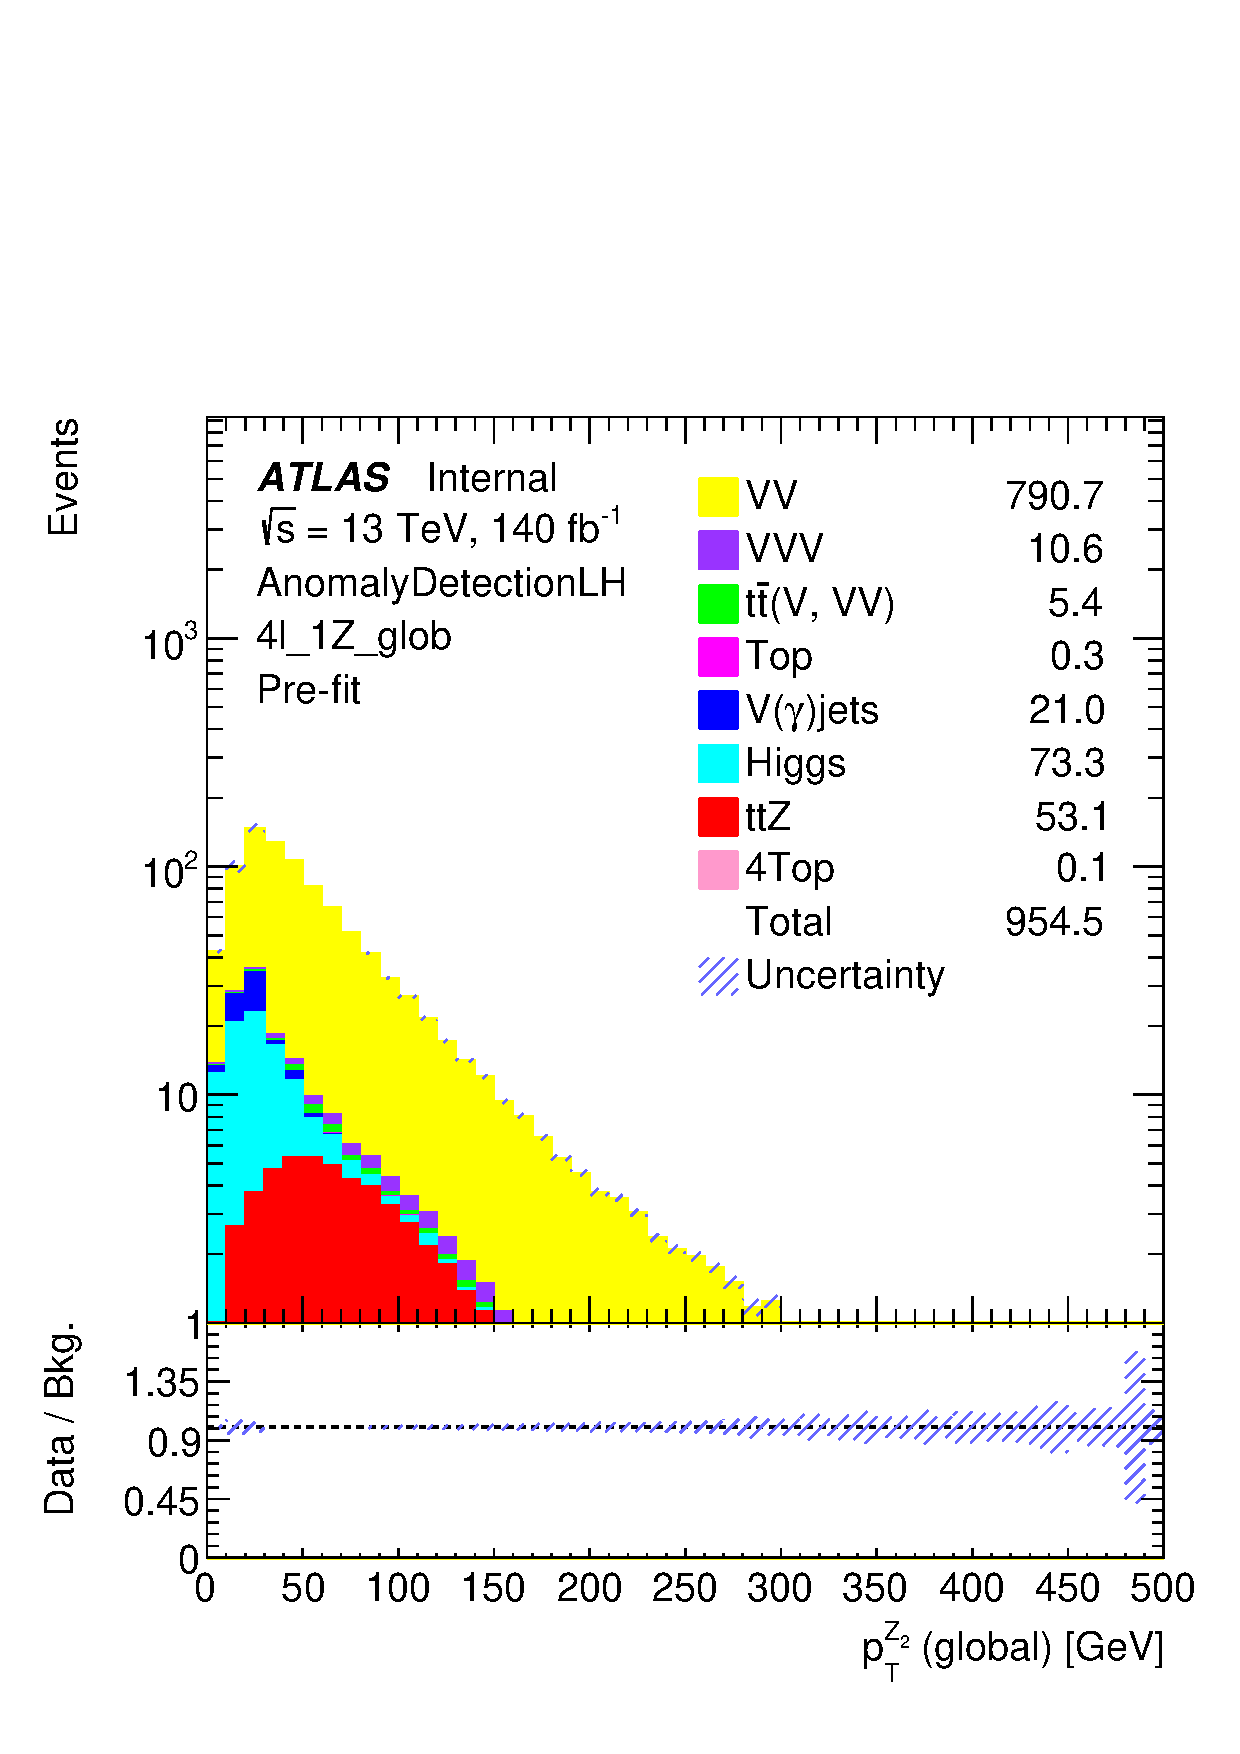
\includegraphics[width=0.24\textwidth]{plots/fourlepLH_run2/Plots/reg_4l_1Z_glob_Z2_pt_glob.pdf}
\end{tabular}
\end{frame}

\begin{frame}{\texttt{Results: 4l\_1Z}}
\begin{tabular}{cccccc}
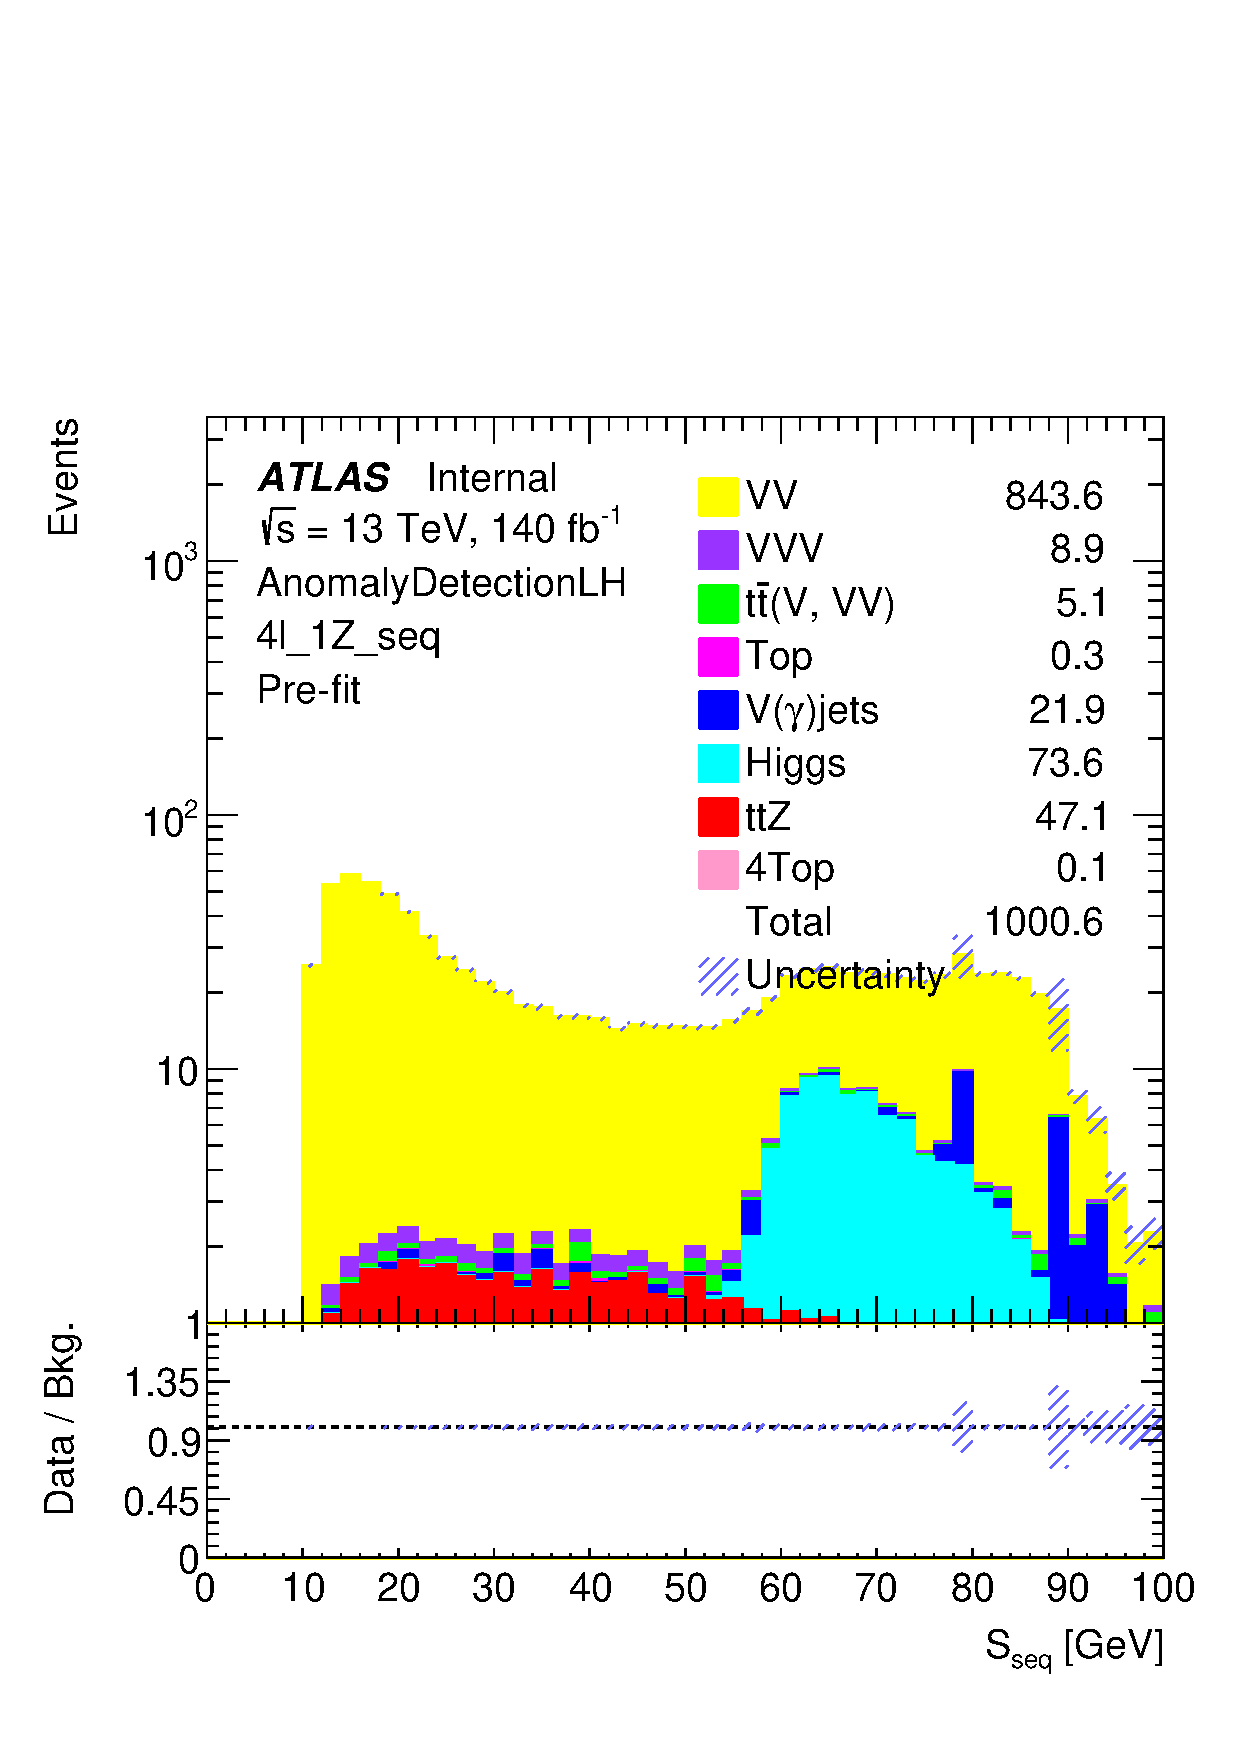
\includegraphics[width=0.24\textwidth]{plots/fourlepLH_run2/Plots/reg_4l_1Z_seq_Zscore_seq.pdf} & 
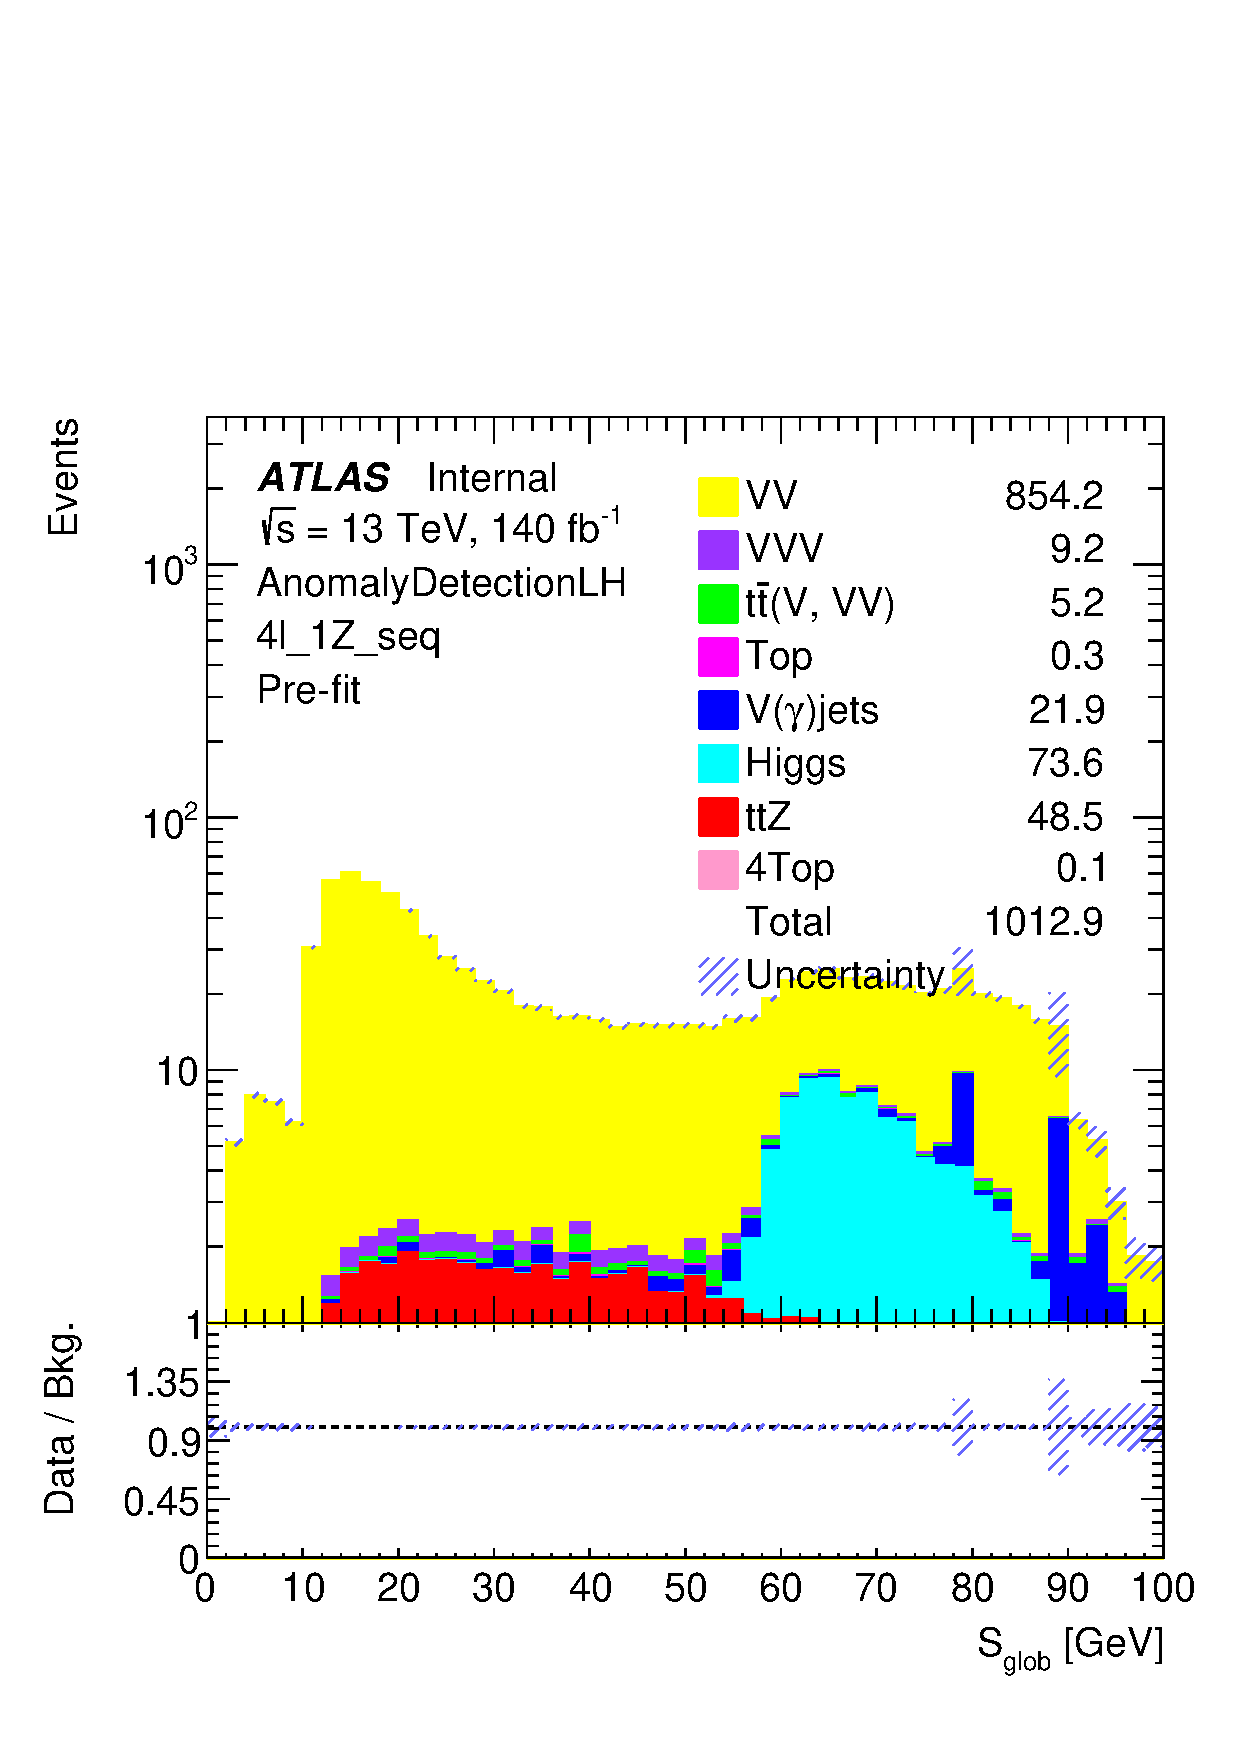
\includegraphics[width=0.24\textwidth]{plots/fourlepLH_run2/Plots/reg_4l_1Z_seq_Zscore_glob.pdf}&
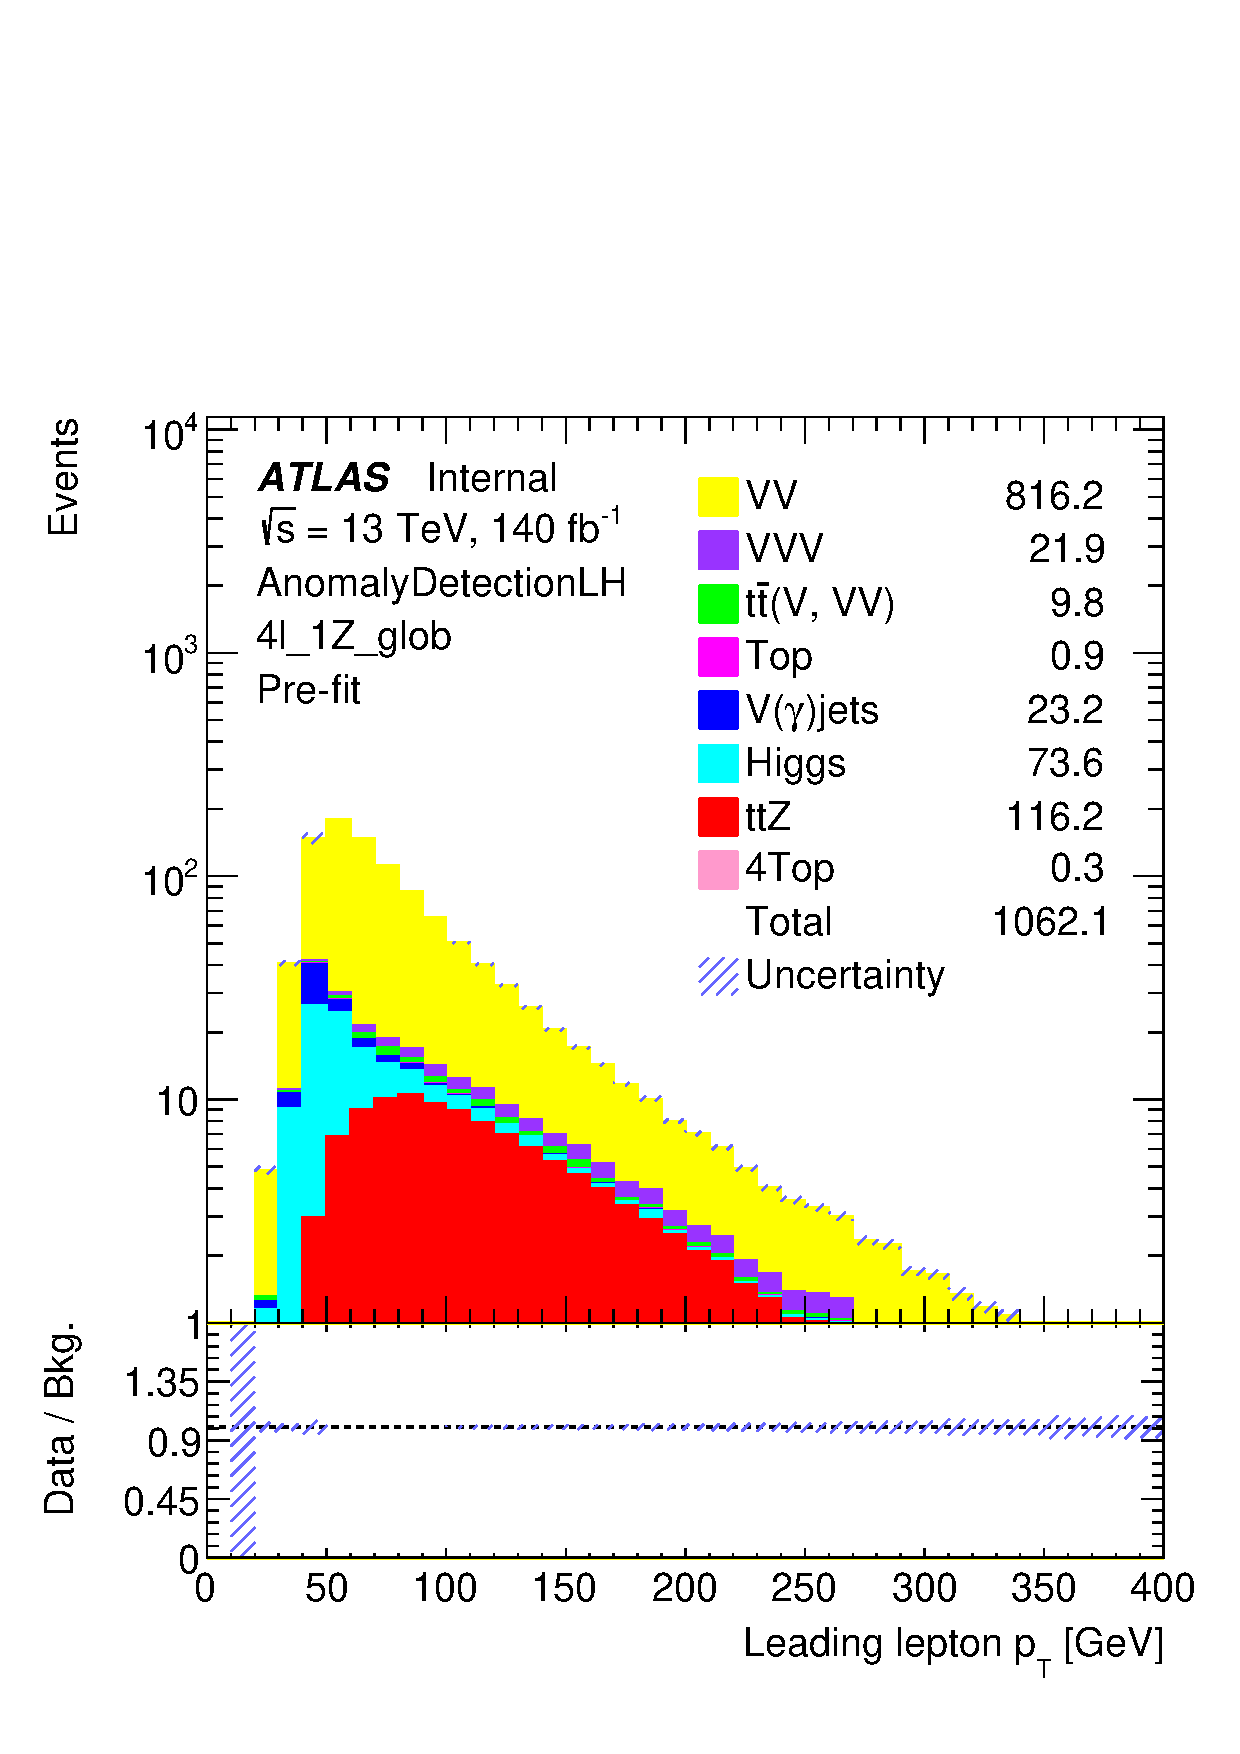
\includegraphics[width=0.24\textwidth]{plots/fourlepLH_run2/Plots/reg_4l_1Z_seq_deltaZscore.pdf}\\

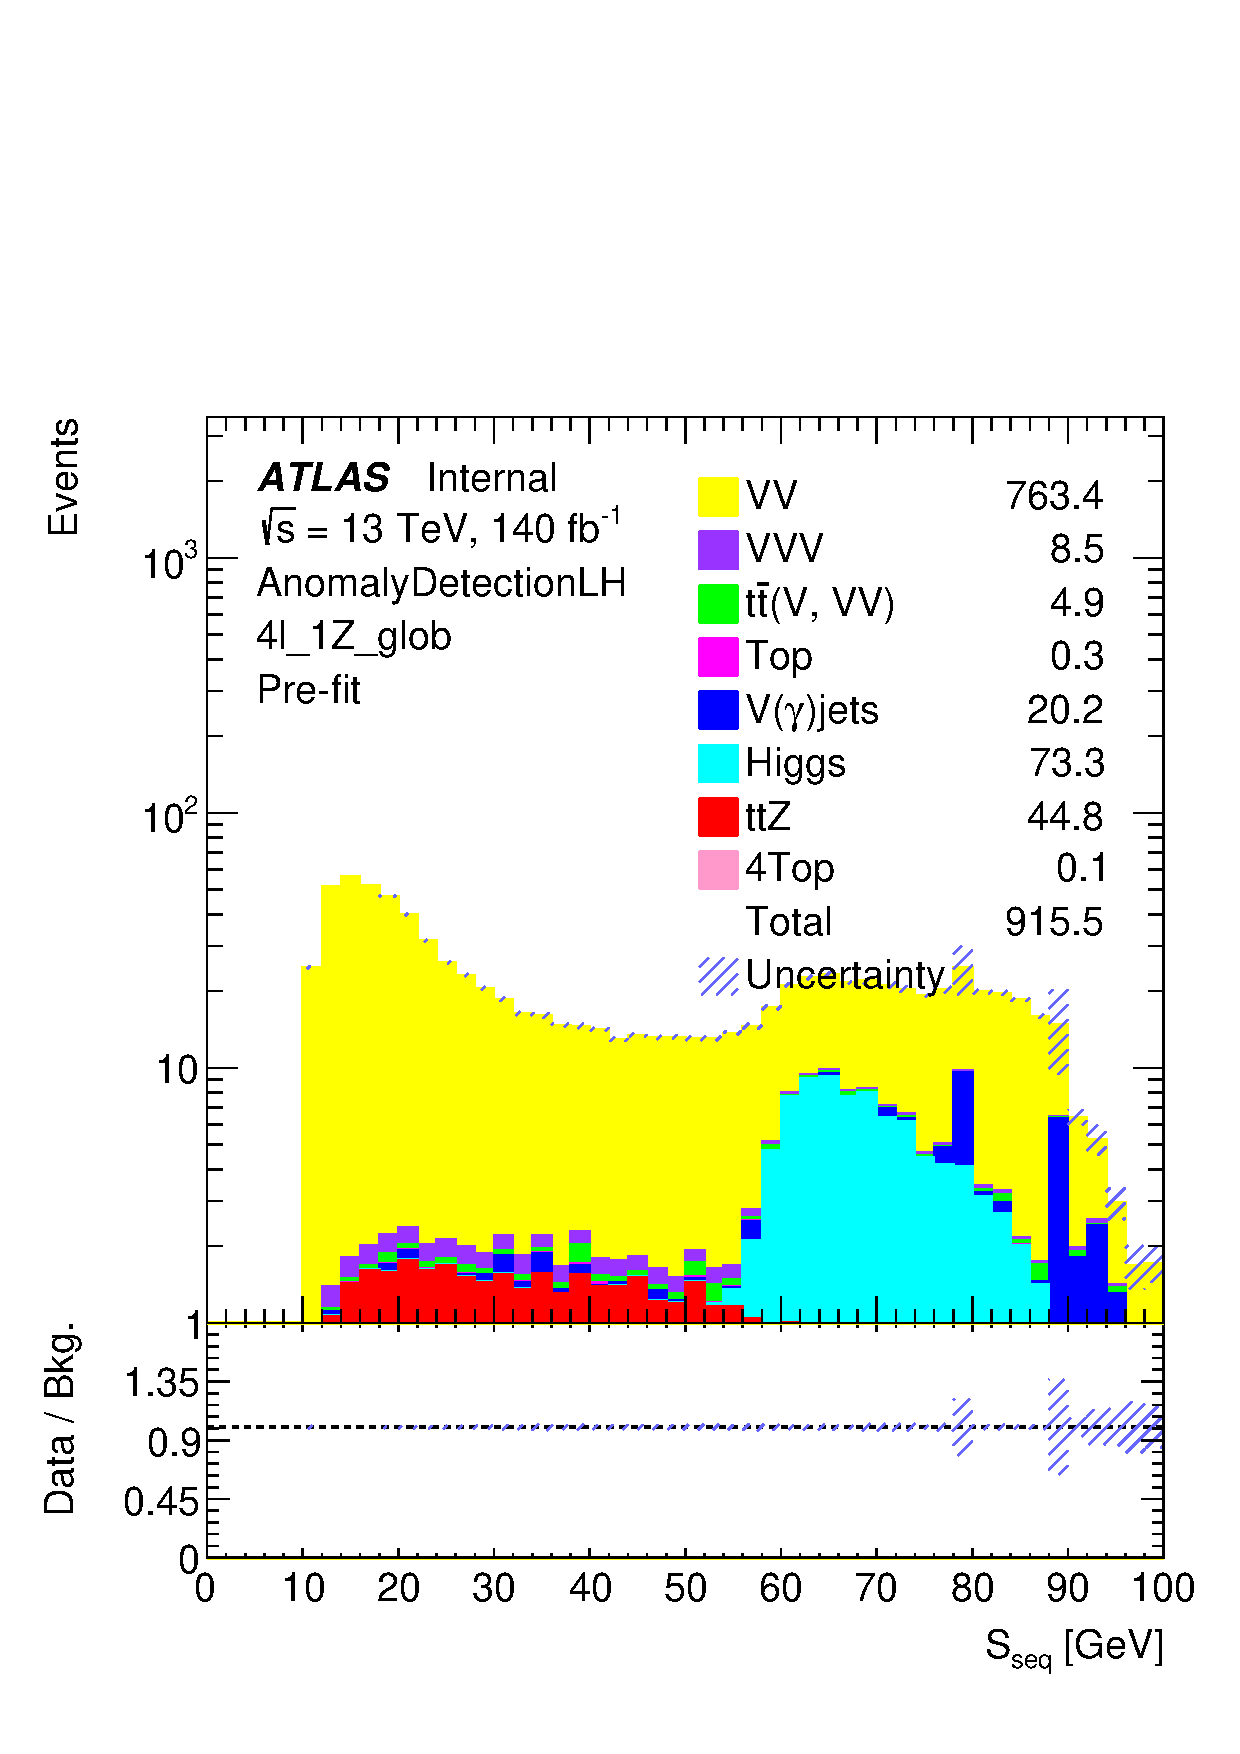
\includegraphics[width=0.24\textwidth]{plots/fourlepLH_run2/Plots/reg_4l_1Z_glob_Zscore_seq.pdf} & 
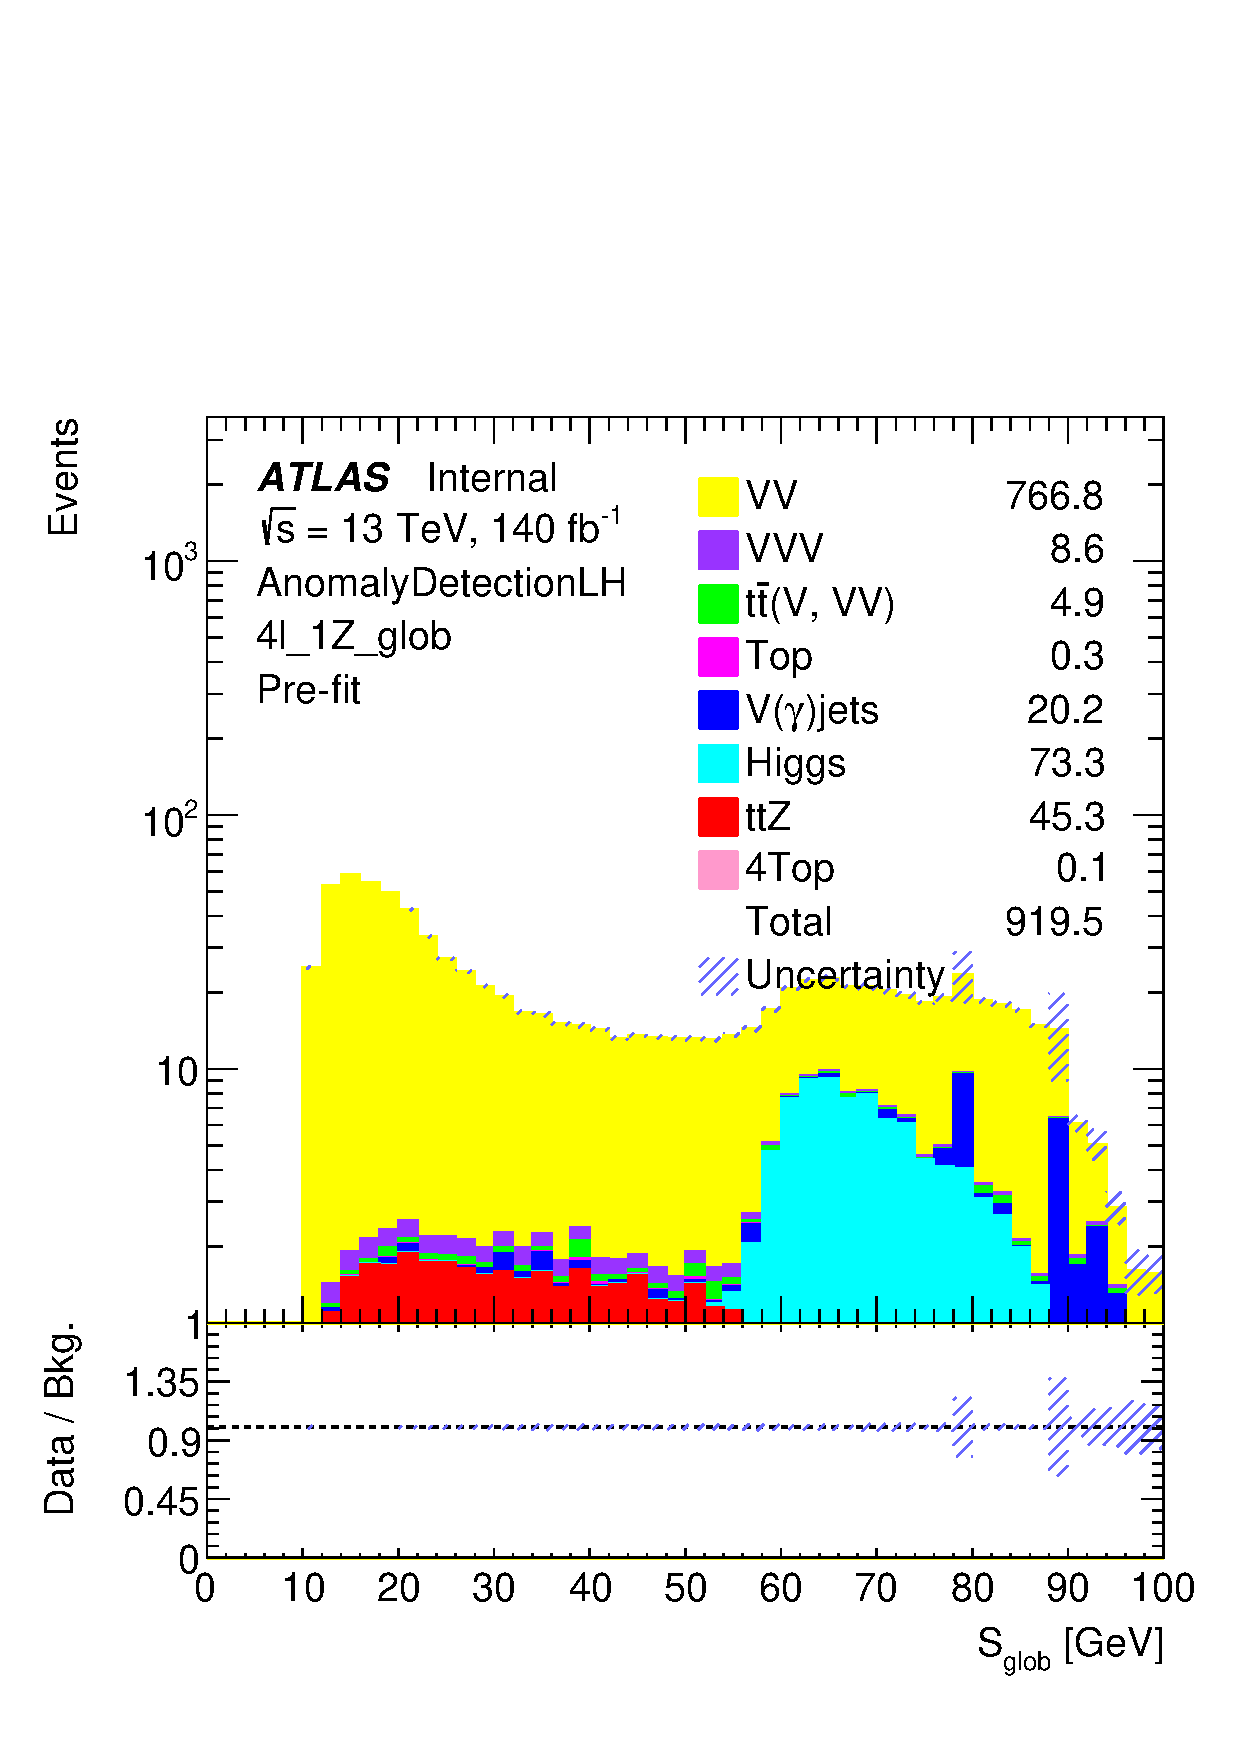
\includegraphics[width=0.24\textwidth]{plots/fourlepLH_run2/Plots/reg_4l_1Z_glob_Zscore_glob.pdf}&
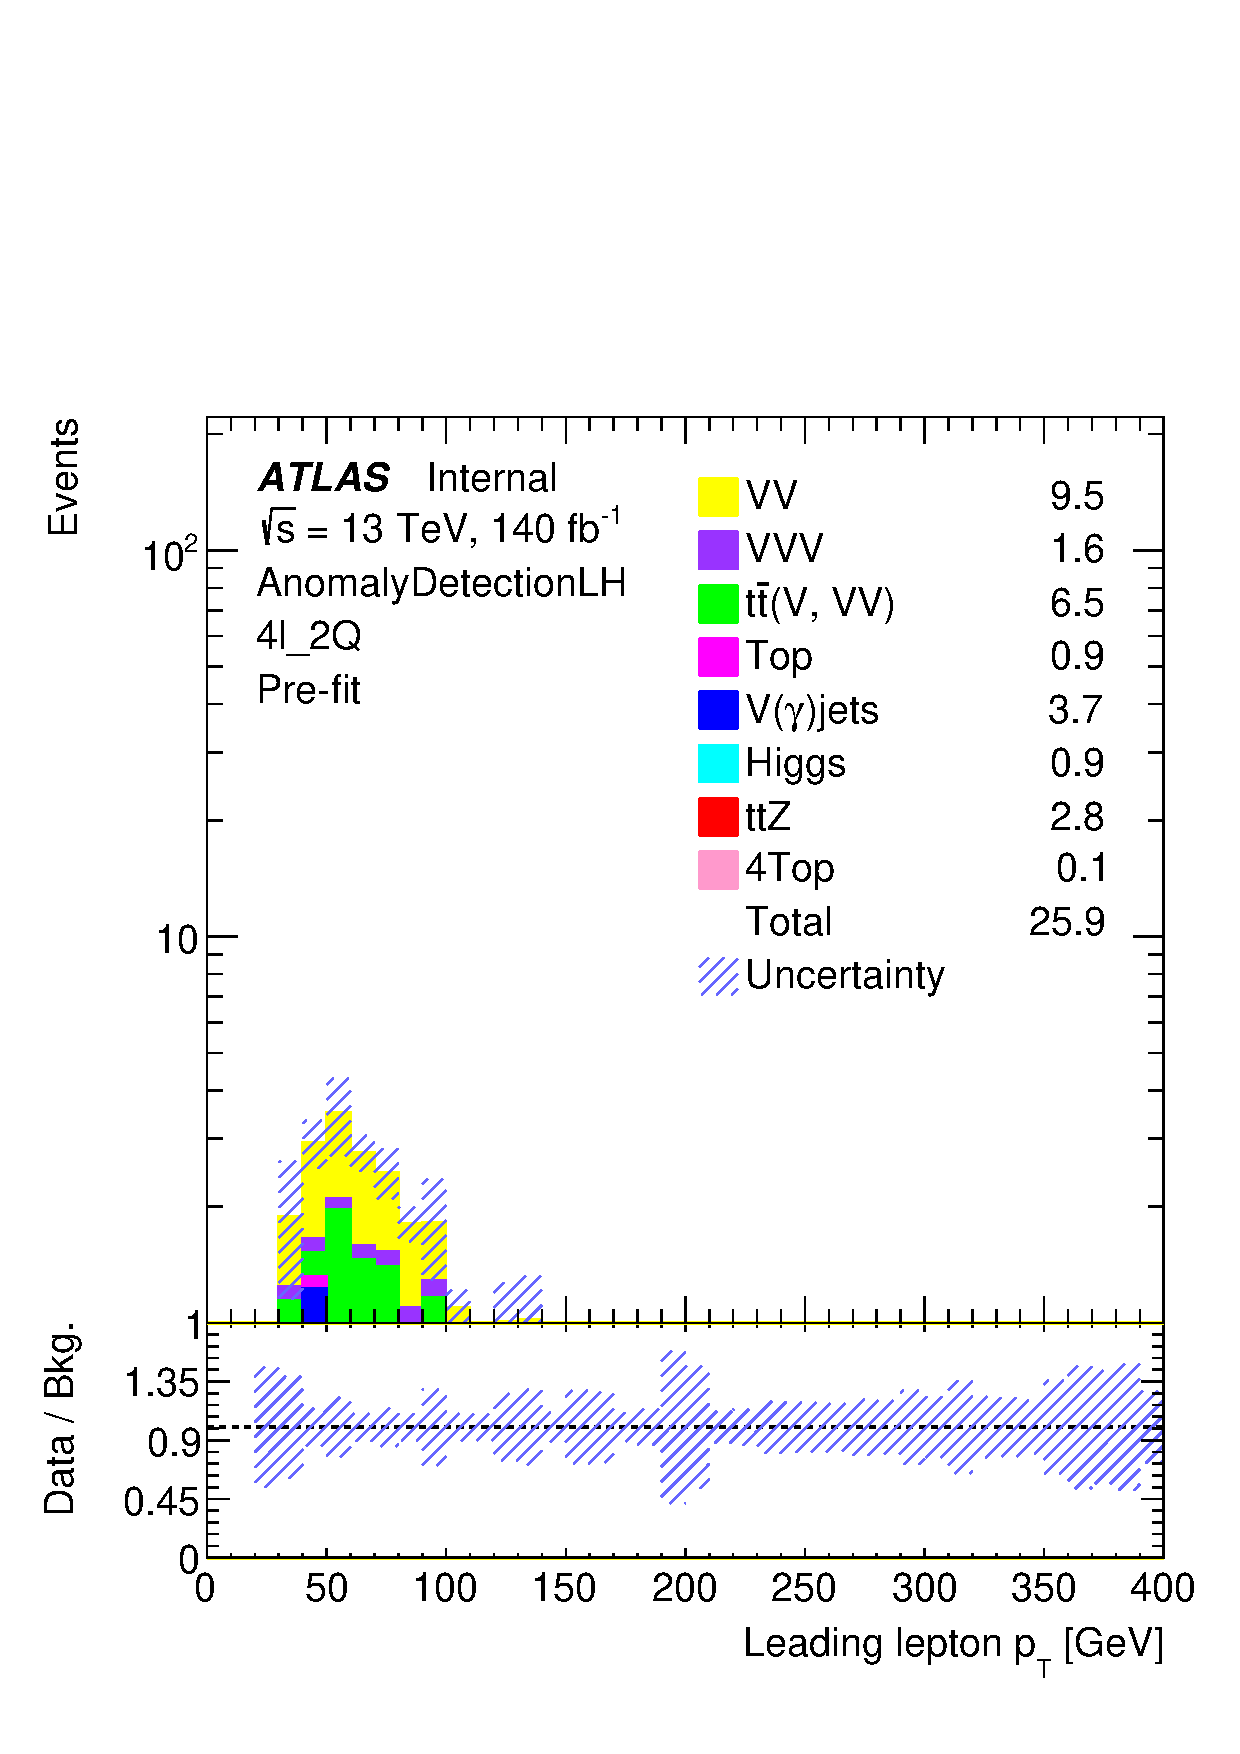
\includegraphics[width=0.24\textwidth]{plots/fourlepLH_run2/Plots/reg_4l_1Z_glob_deltaZscore.pdf}
\end{tabular}
\end{frame}


\begin{frame}{\texttt{Results: 4l\_1Z}}
\begin{tabular}{cccccc}

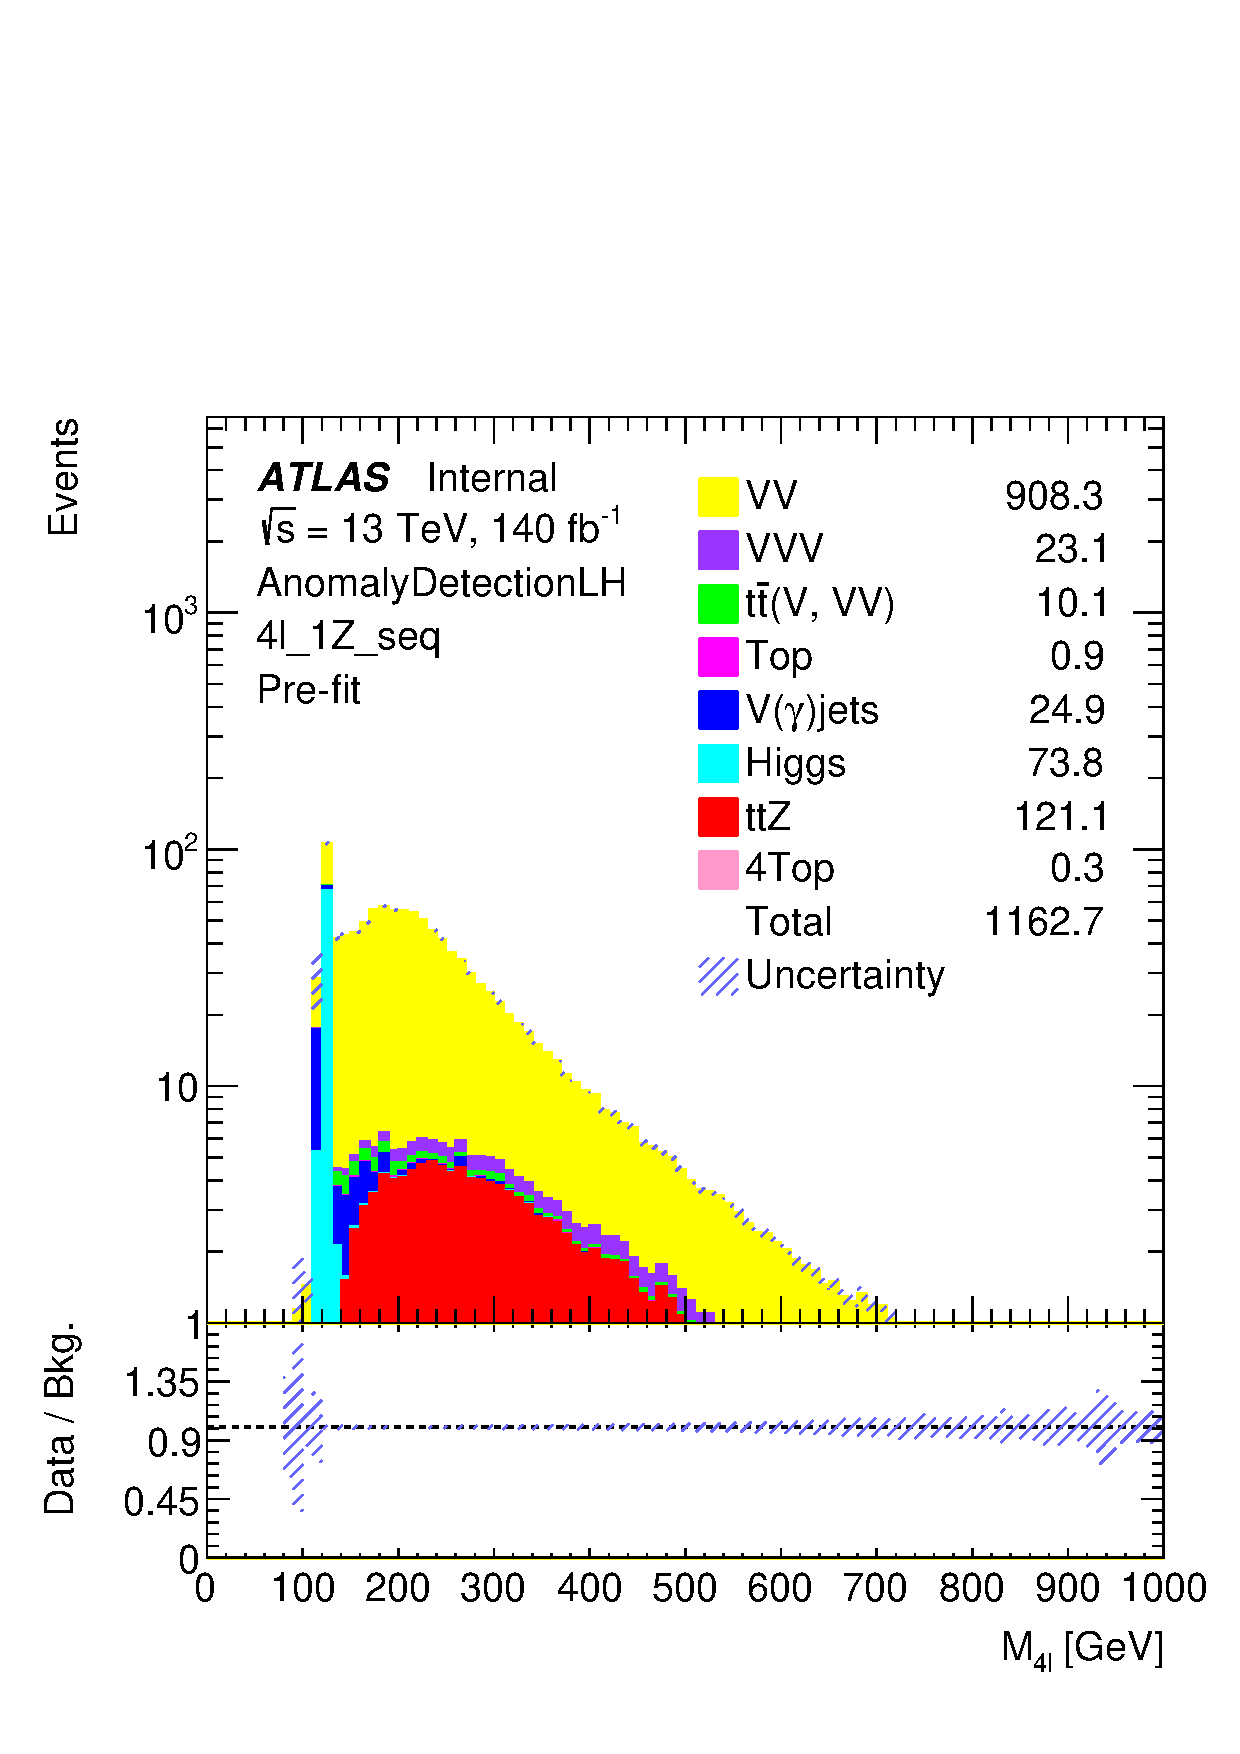
\includegraphics[width=0.24\textwidth]{plots/fourlepLH_run2/Plots/reg_4l_1Z_seq_m4l.pdf} &
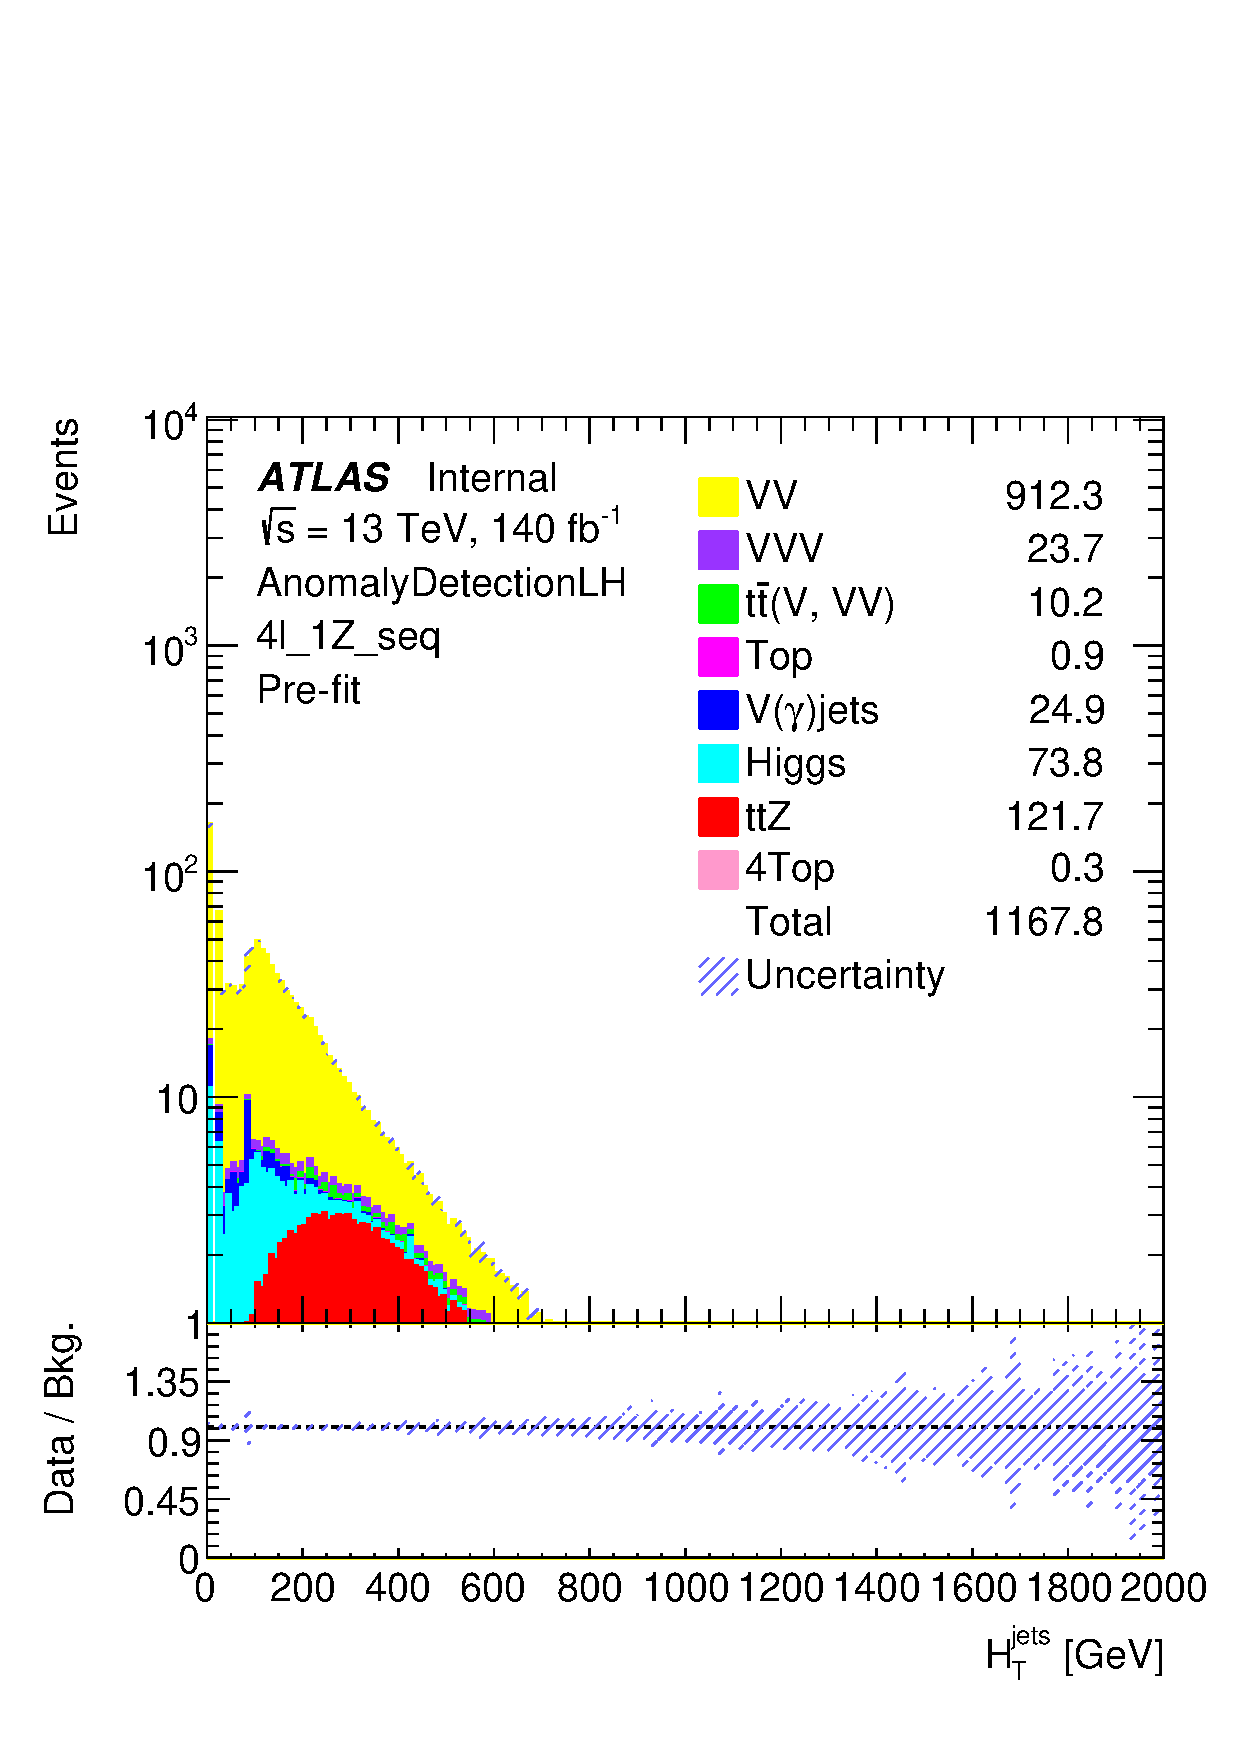
\includegraphics[width=0.24\textwidth]{plots/fourlepLH_run2/Plots/reg_4l_1Z_seq_HT_jets.pdf} &
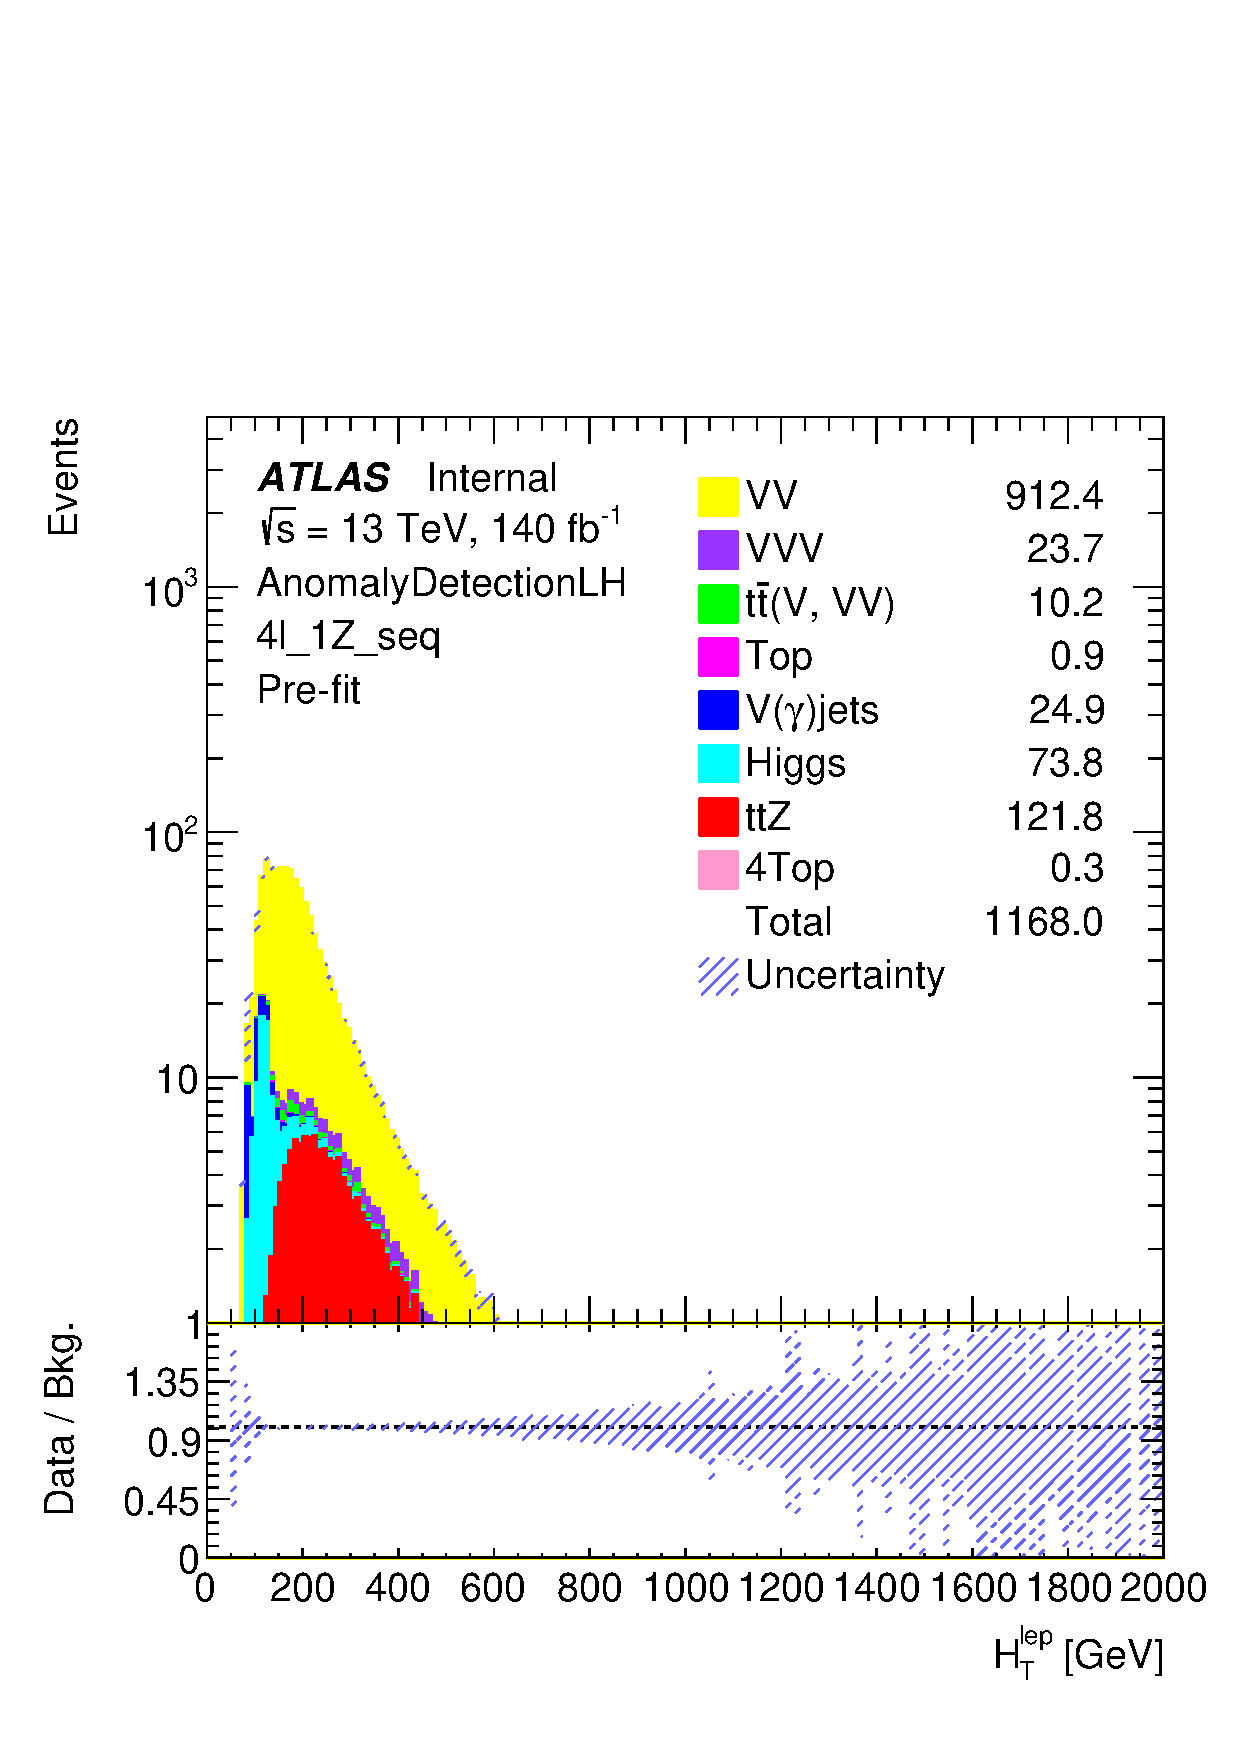
\includegraphics[width=0.24\textwidth]{plots/fourlepLH_run2/Plots/reg_4l_1Z_seq_HT_lep.pdf} &
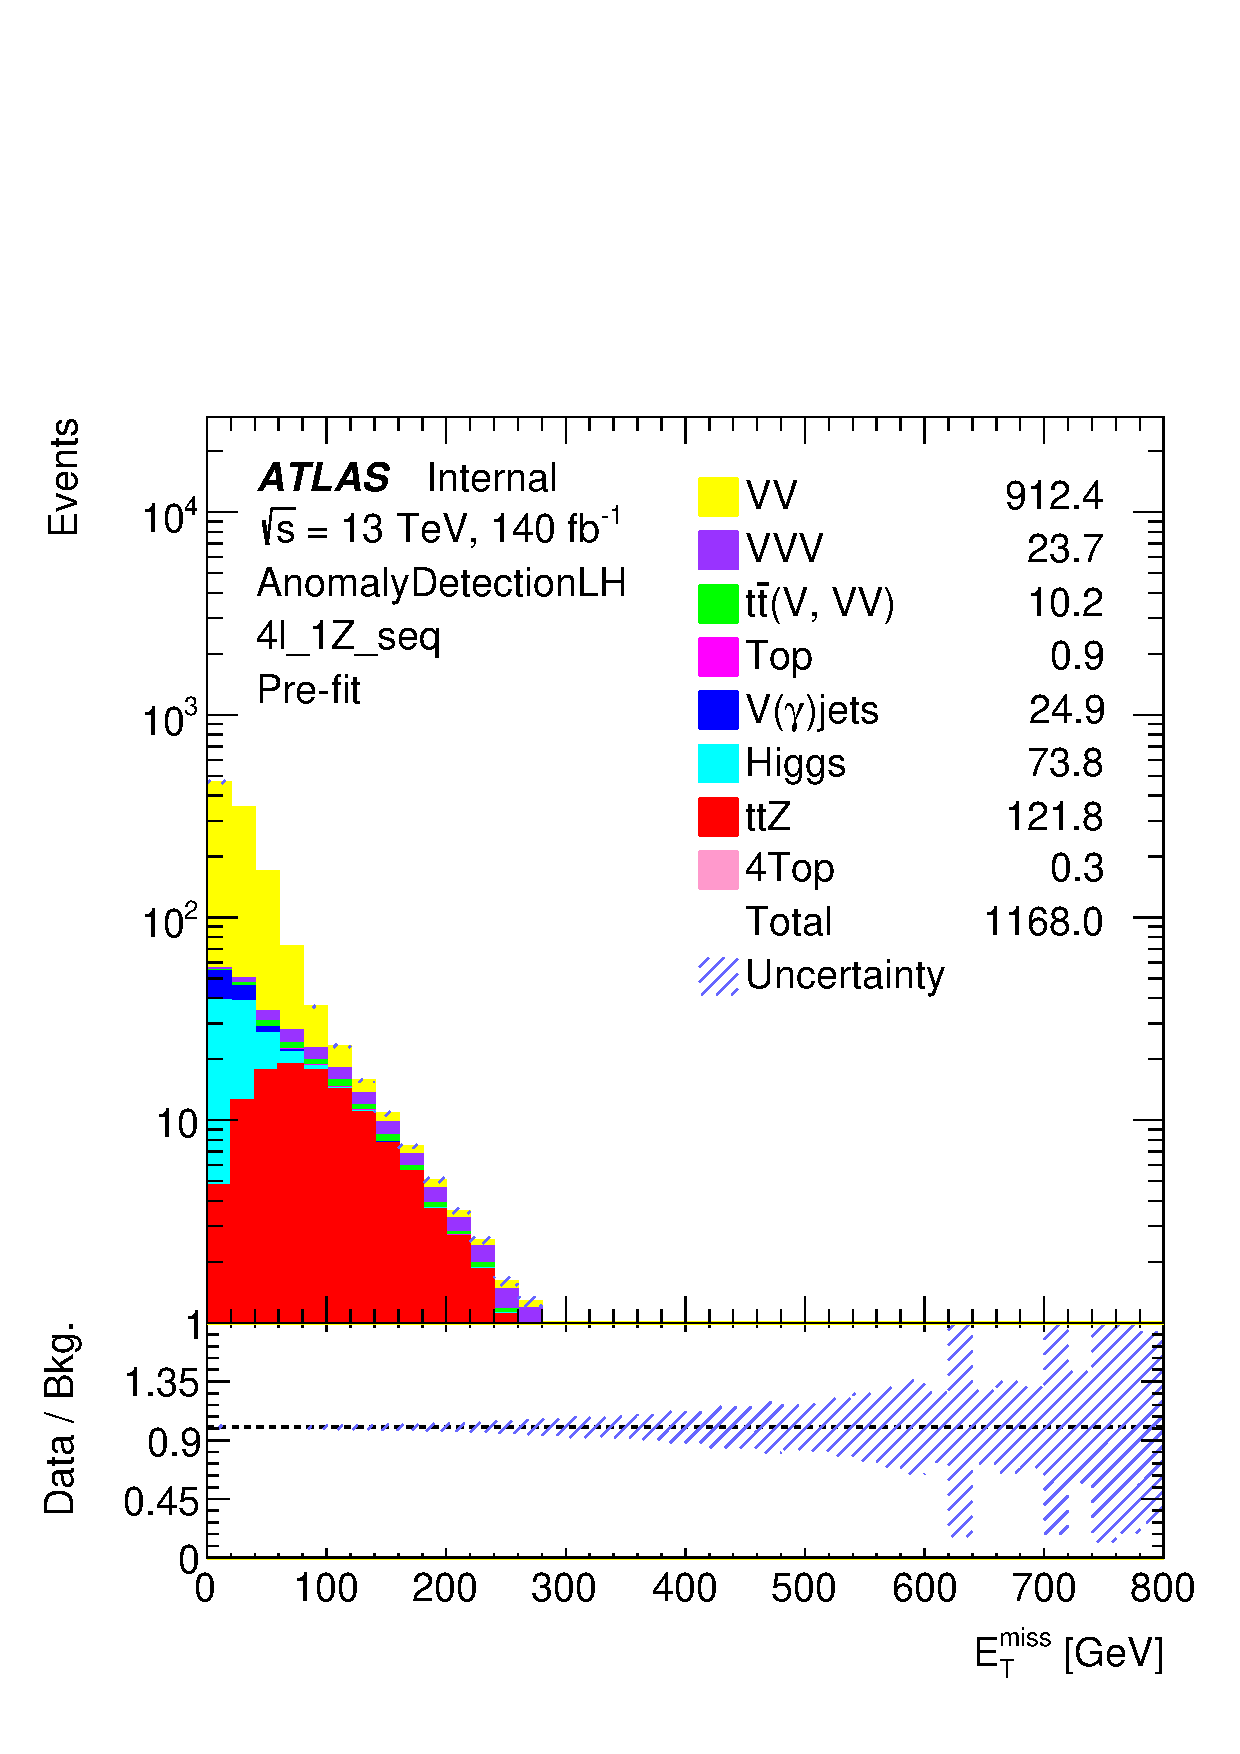
\includegraphics[width=0.24\textwidth]{plots/fourlepLH_run2/Plots/reg_4l_1Z_seq_met.pdf} \\

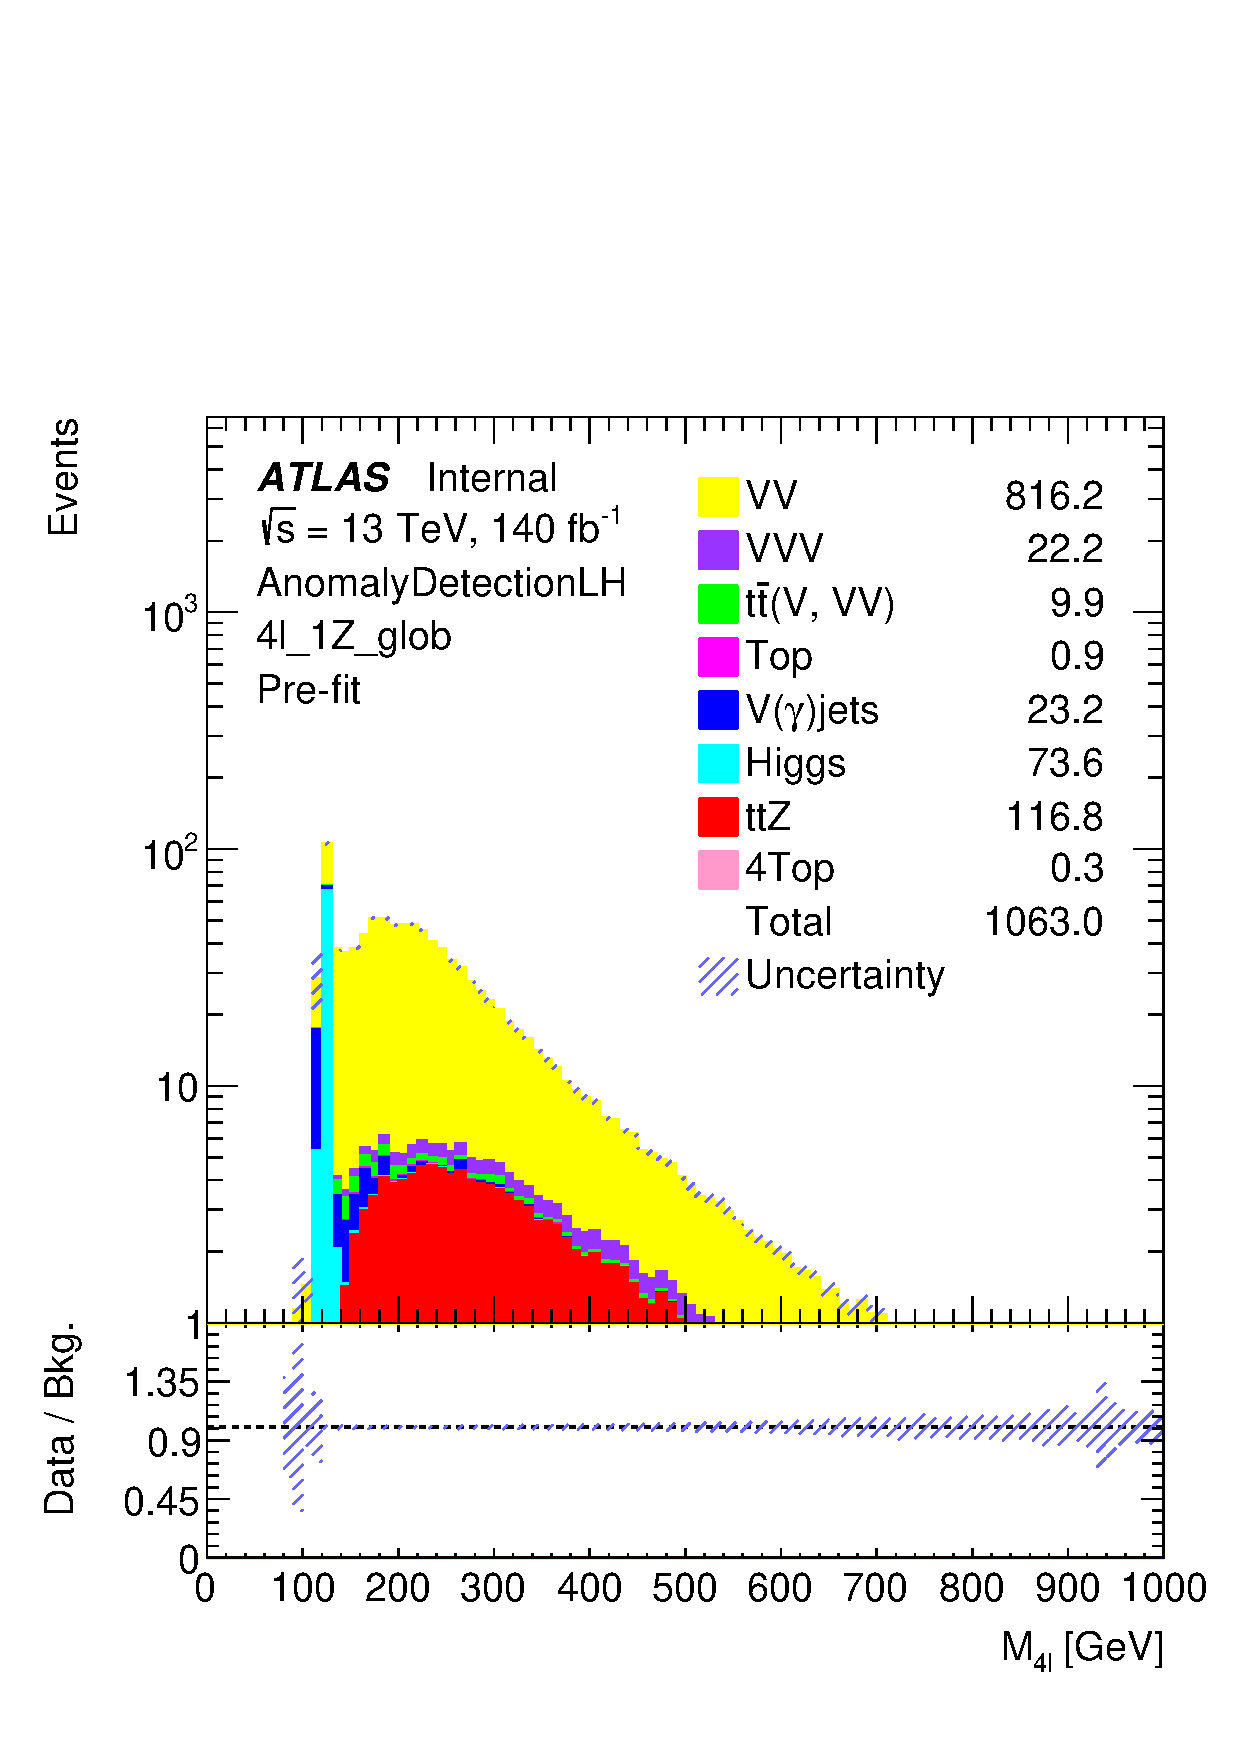
\includegraphics[width=0.24\textwidth]{plots/fourlepLH_run2/Plots/reg_4l_1Z_glob_m4l.pdf} &
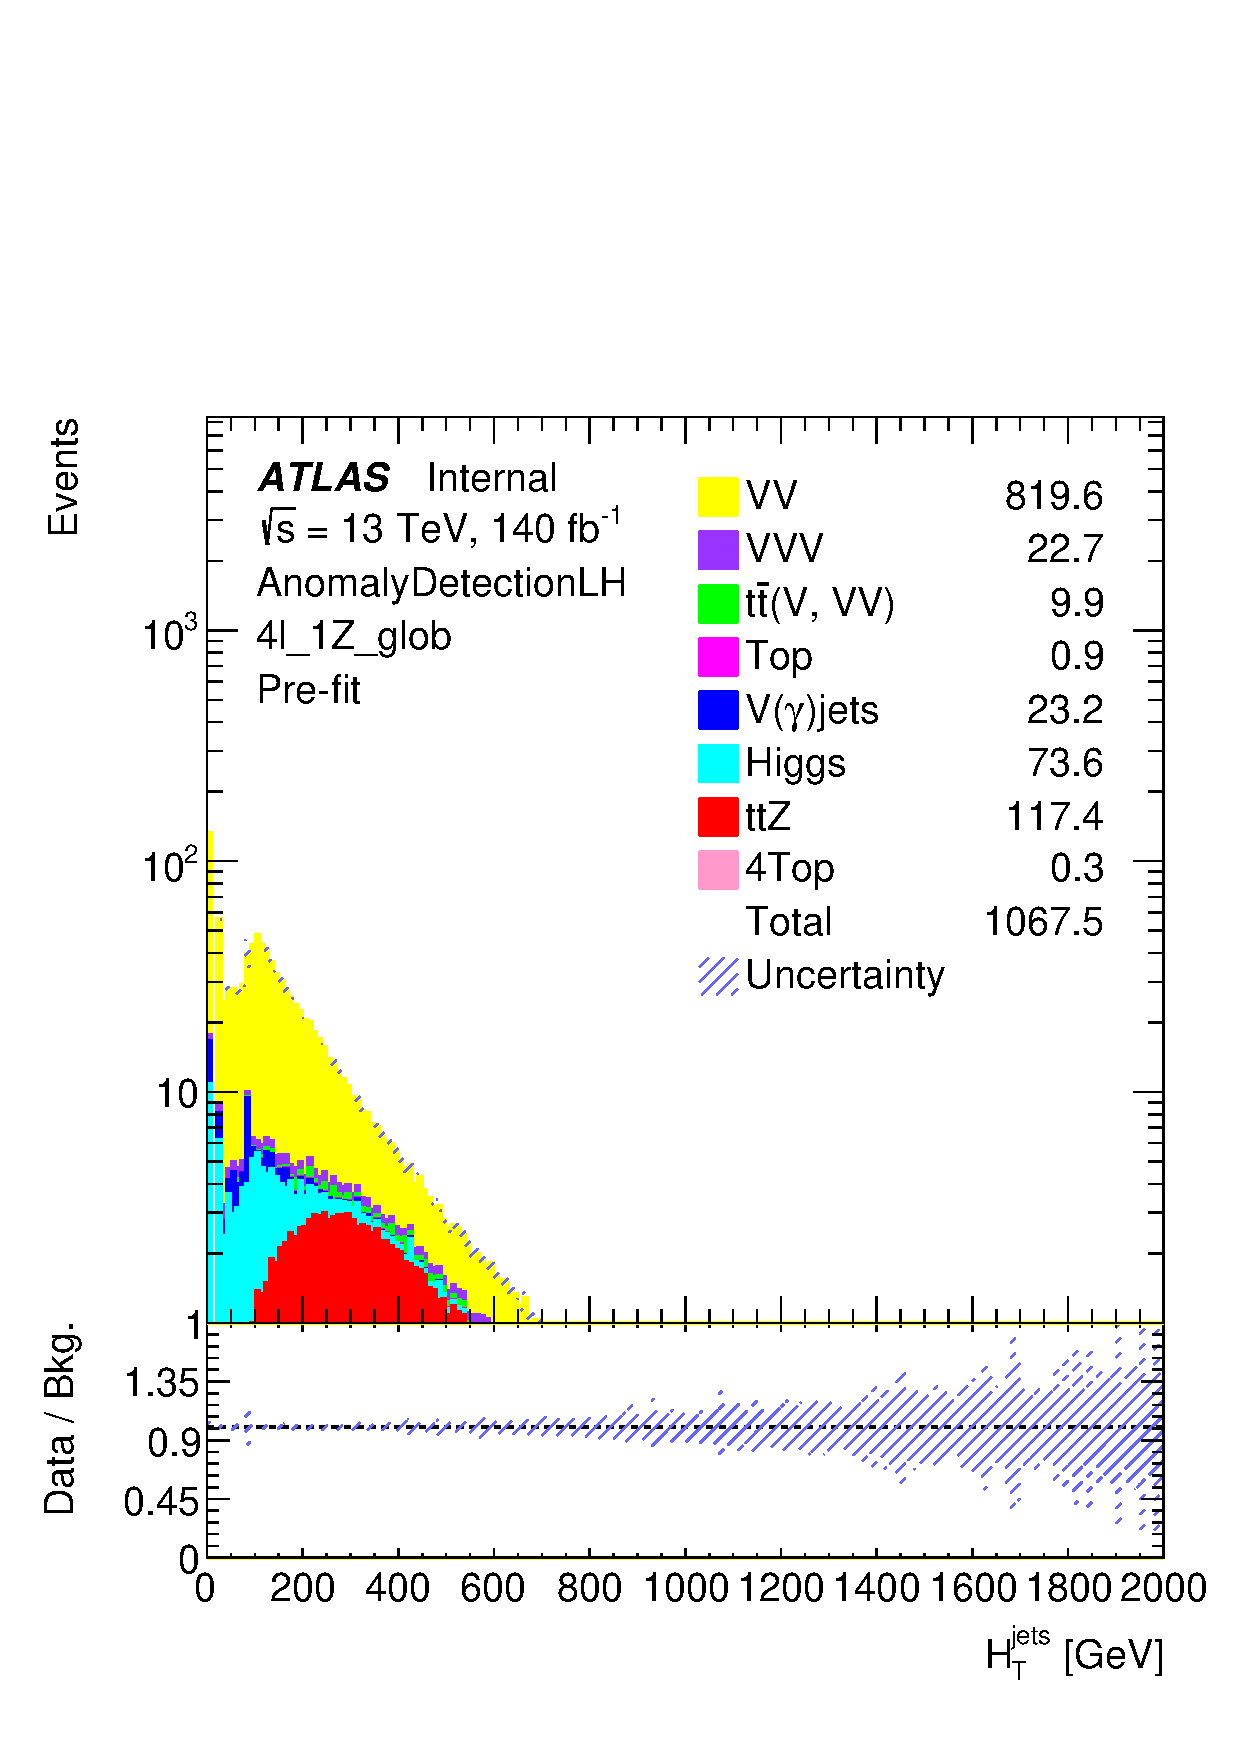
\includegraphics[width=0.24\textwidth]{plots/fourlepLH_run2/Plots/reg_4l_1Z_glob_HT_jets.pdf} &
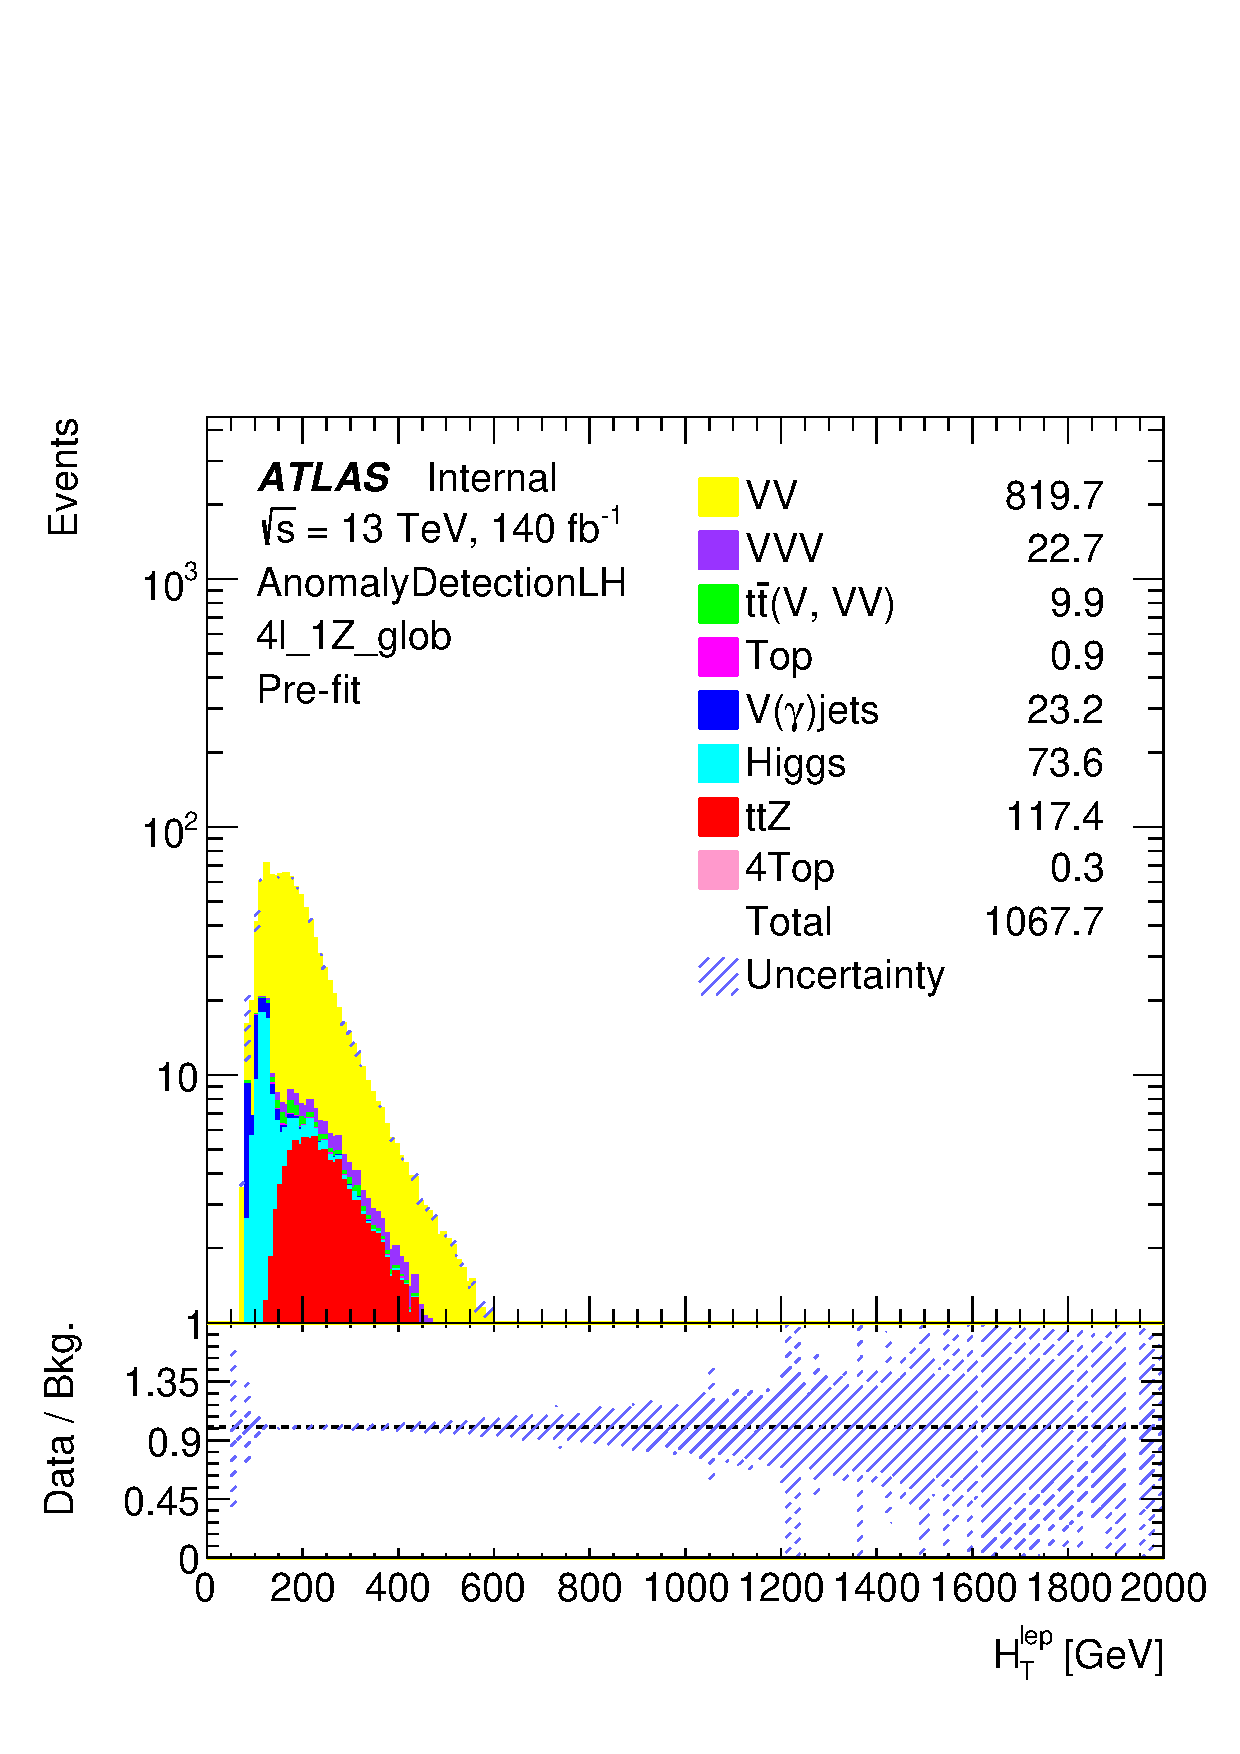
\includegraphics[width=0.24\textwidth]{plots/fourlepLH_run2/Plots/reg_4l_1Z_glob_HT_lep.pdf} &
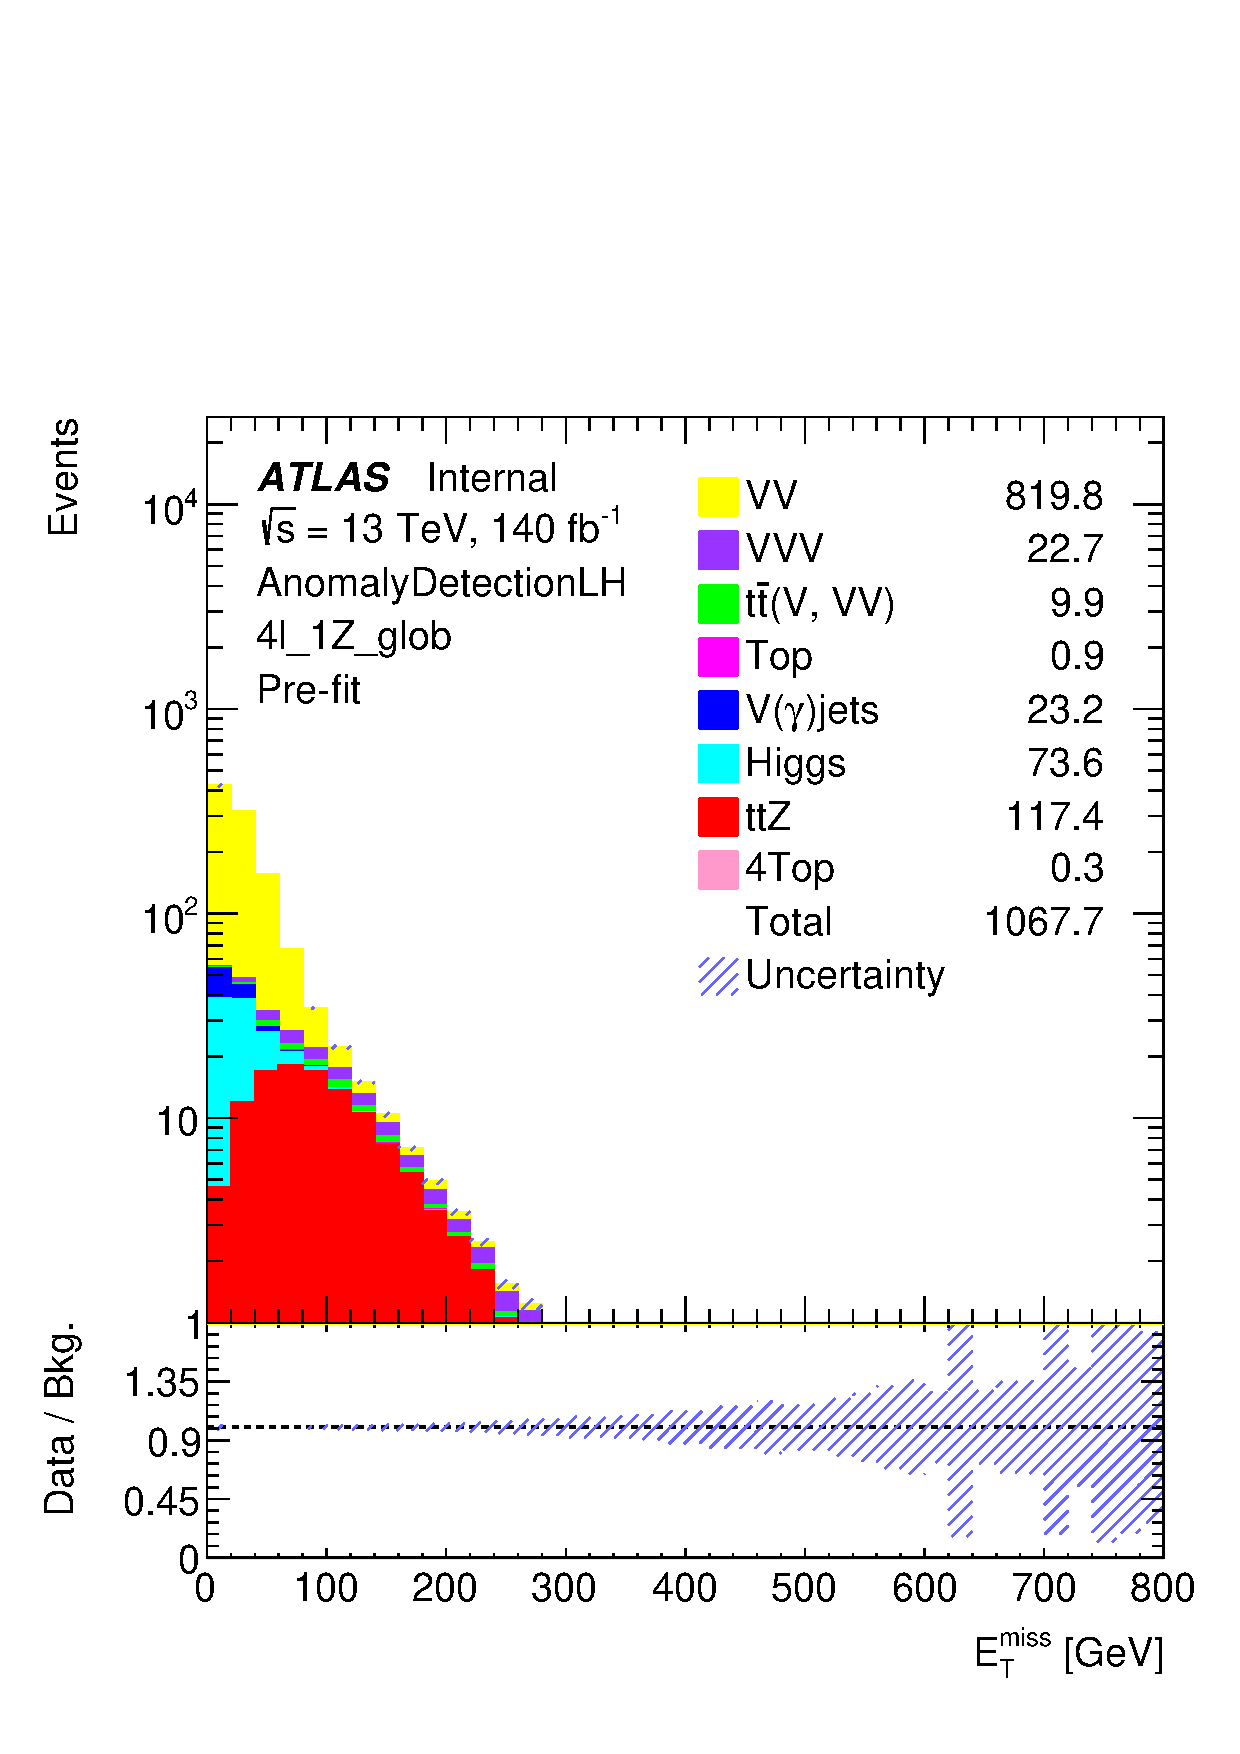
\includegraphics[width=0.24\textwidth]{plots/fourlepLH_run2/Plots/reg_4l_1Z_glob_met.pdf} \\

\end{tabular}
\end{frame}

\begin{frame}{\texttt{Results: 4l\_1Z}}
\begin{tabular}{cccccc}
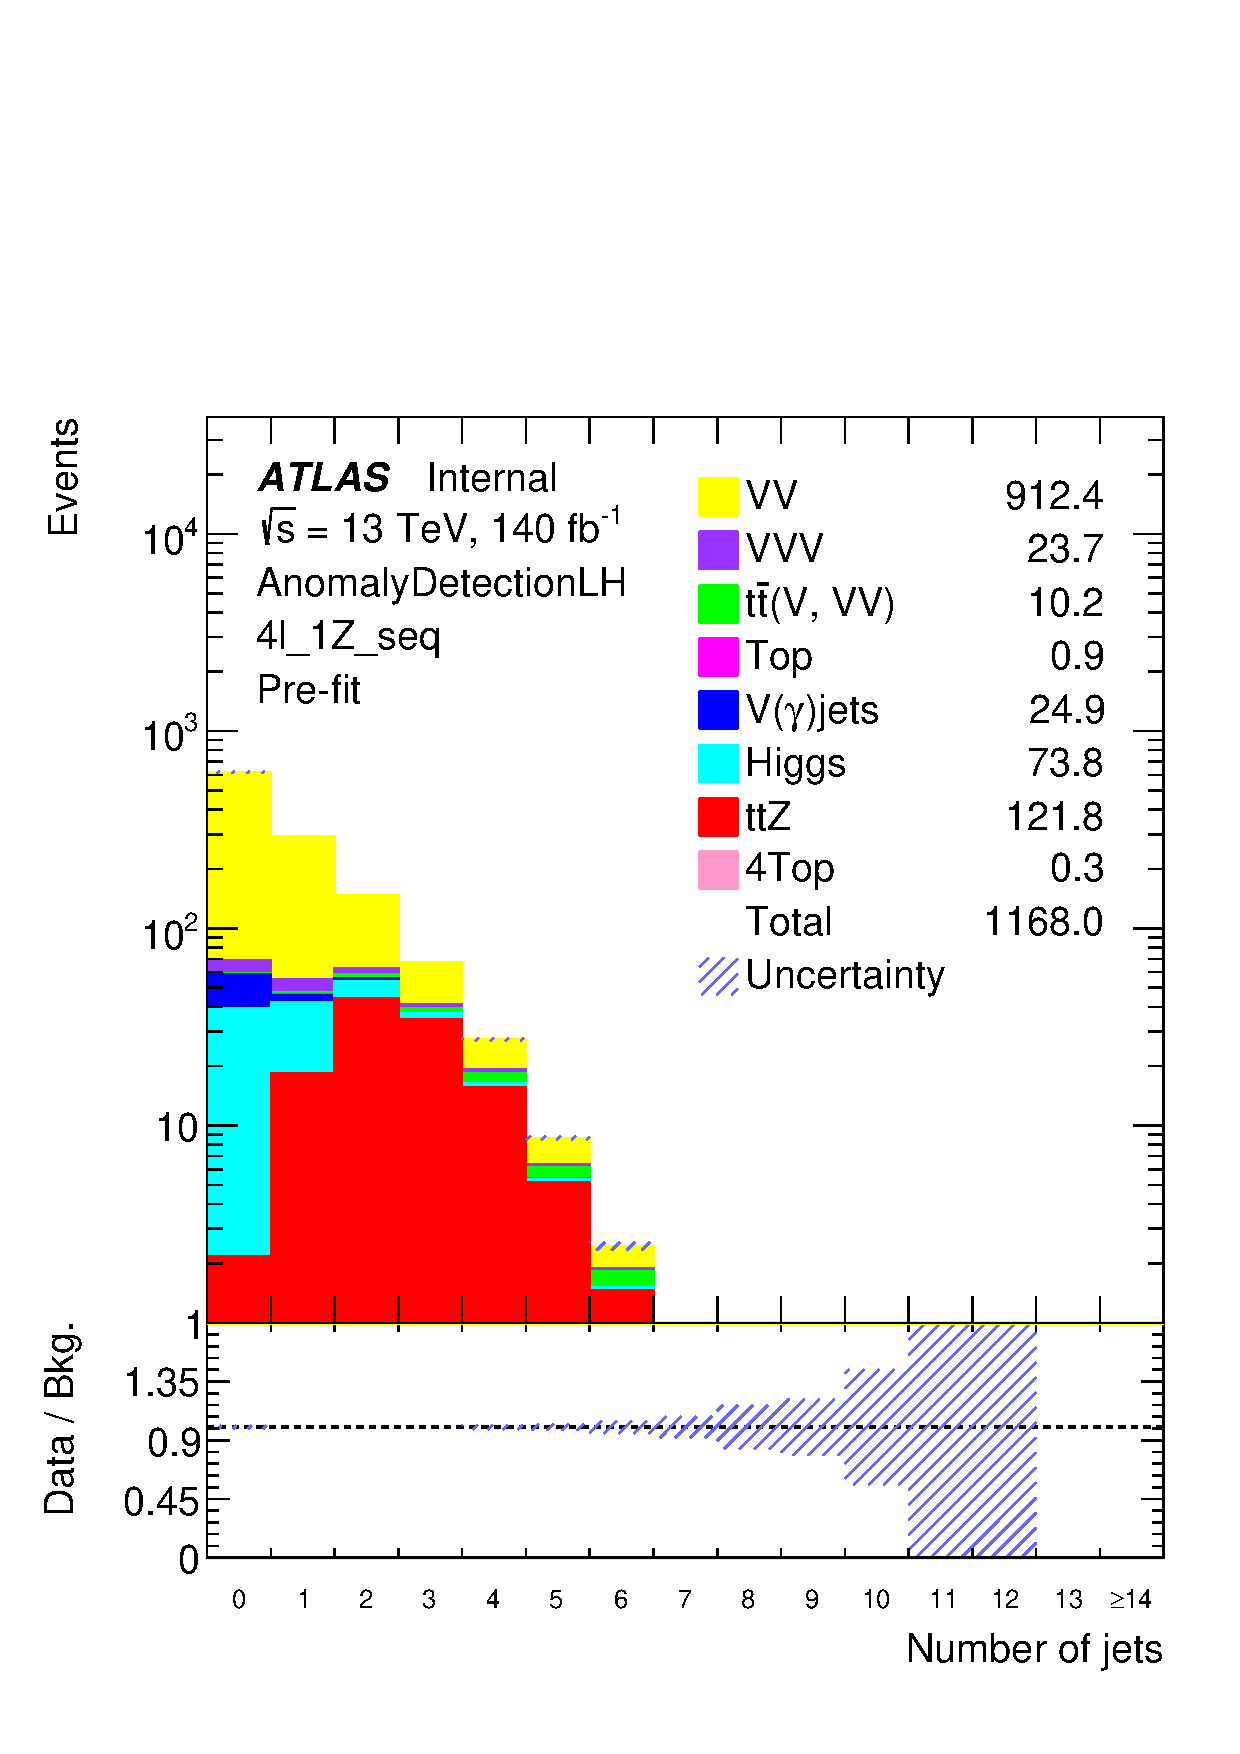
\includegraphics[width=0.24\textwidth]{plots/fourlepLH_run2/Plots/reg_4l_1Z_seq_nJets.pdf} &
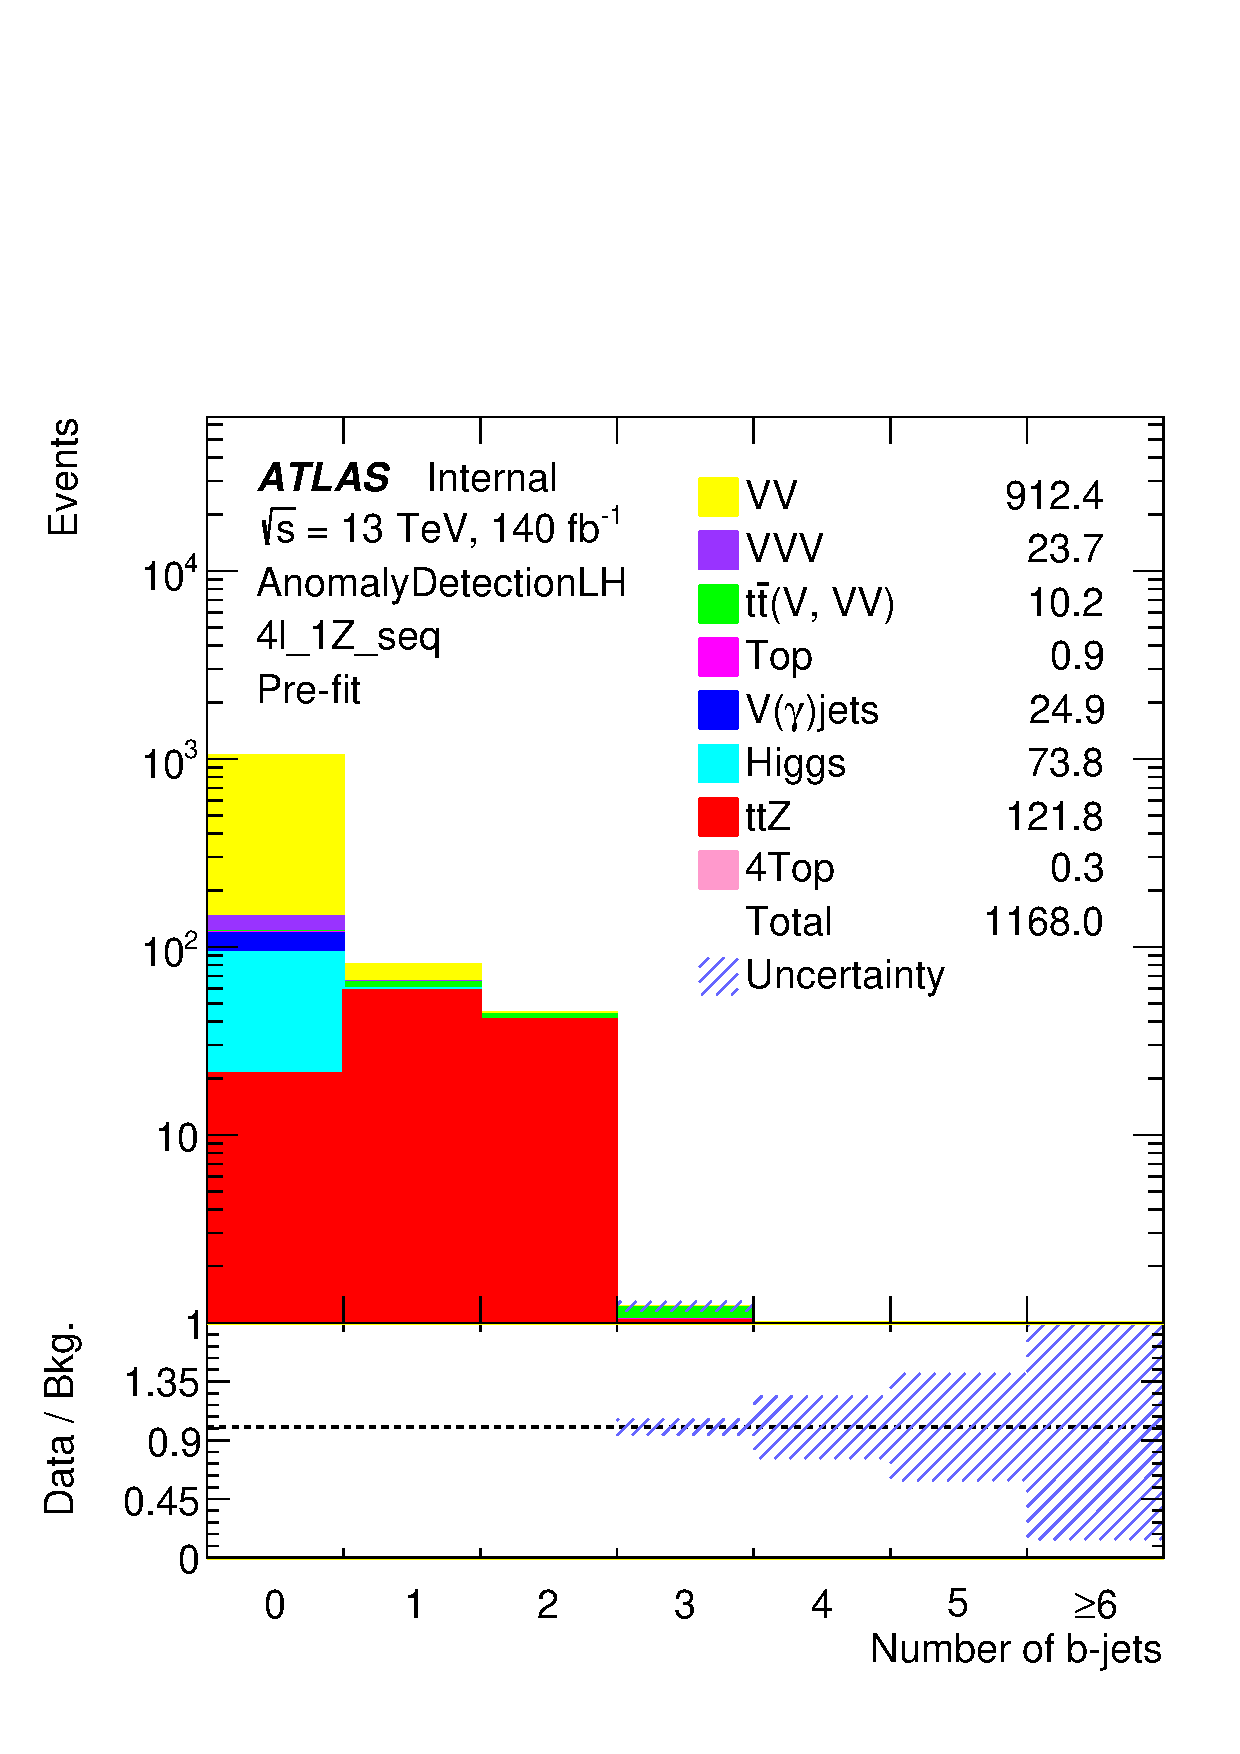
\includegraphics[width=0.24\textwidth]{plots/fourlepLH_run2/Plots/reg_4l_1Z_seq_nbJets.pdf} &
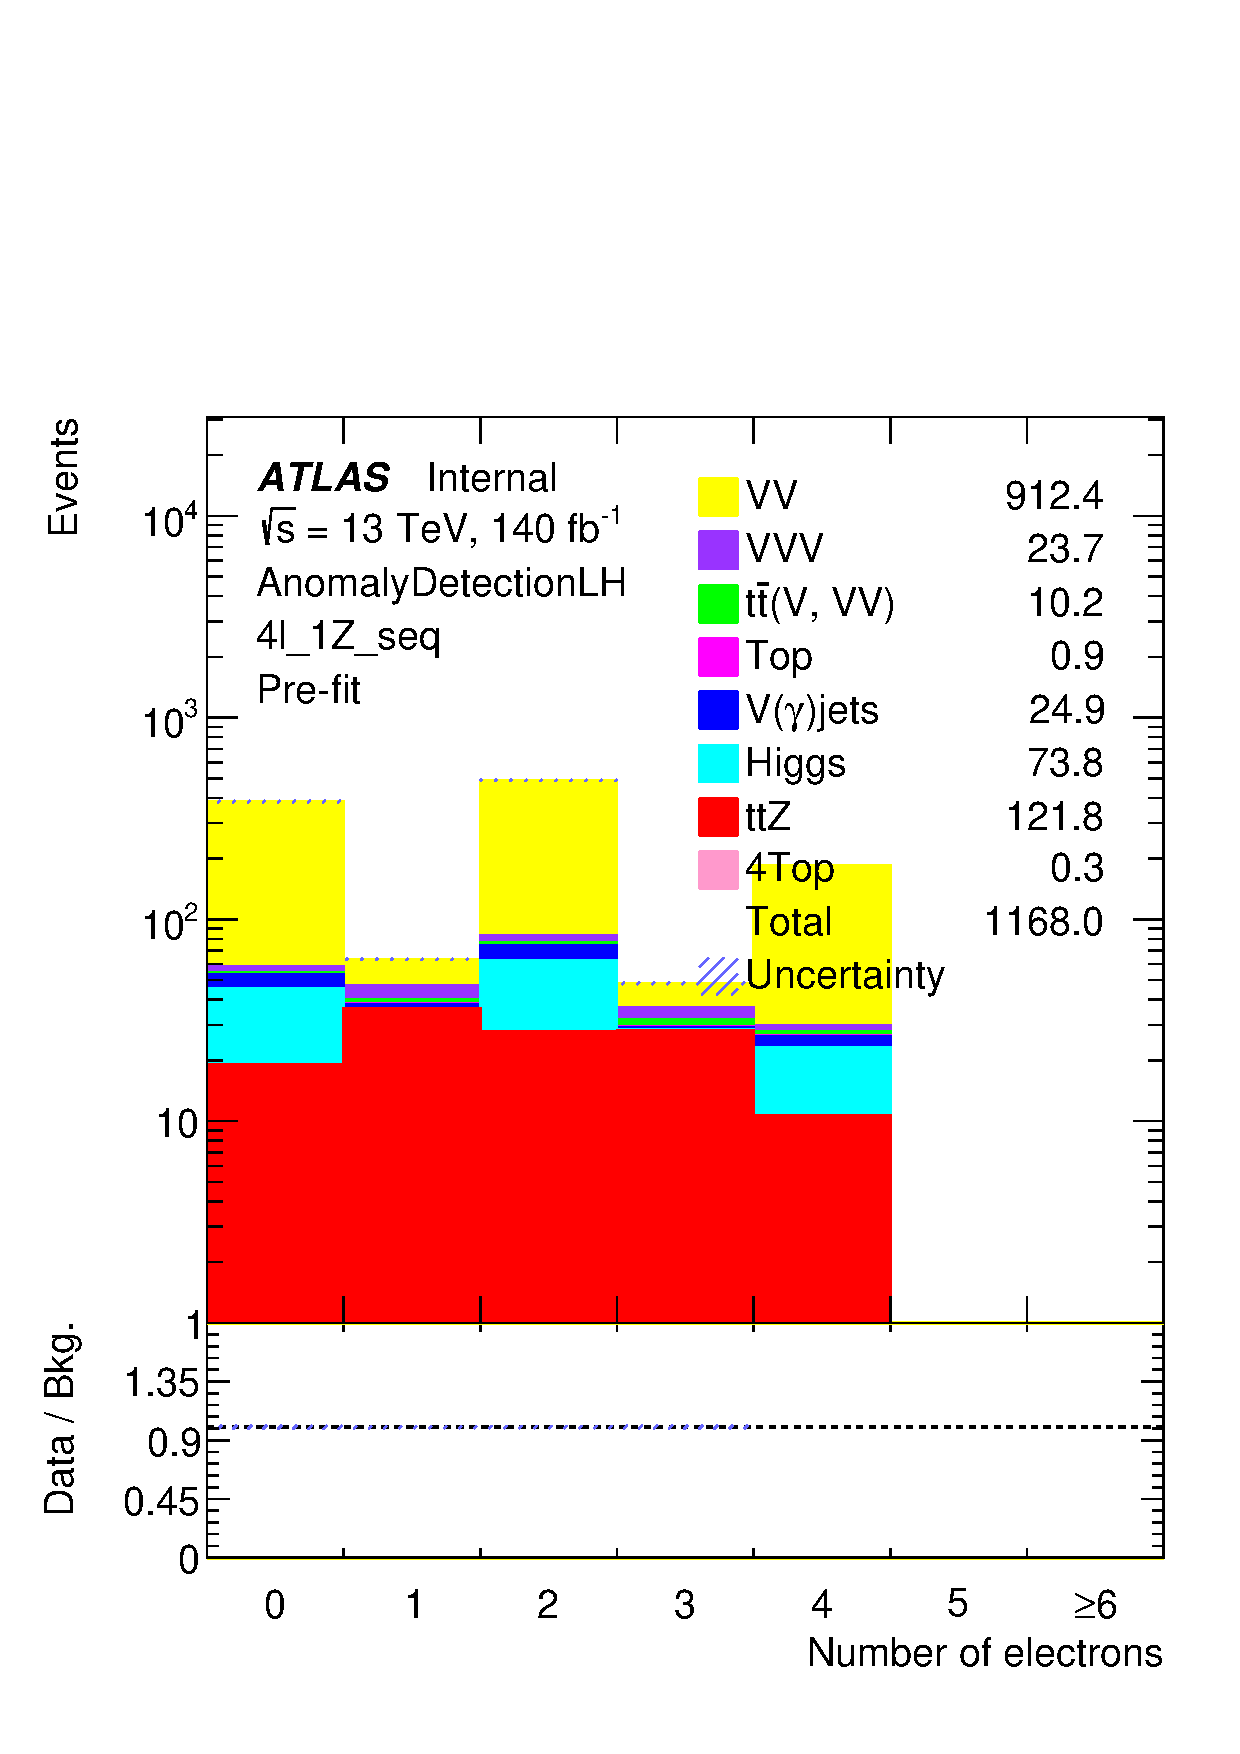
\includegraphics[width=0.24\textwidth]{plots/fourlepLH_run2/Plots/reg_4l_1Z_seq_nElectrons.pdf} &
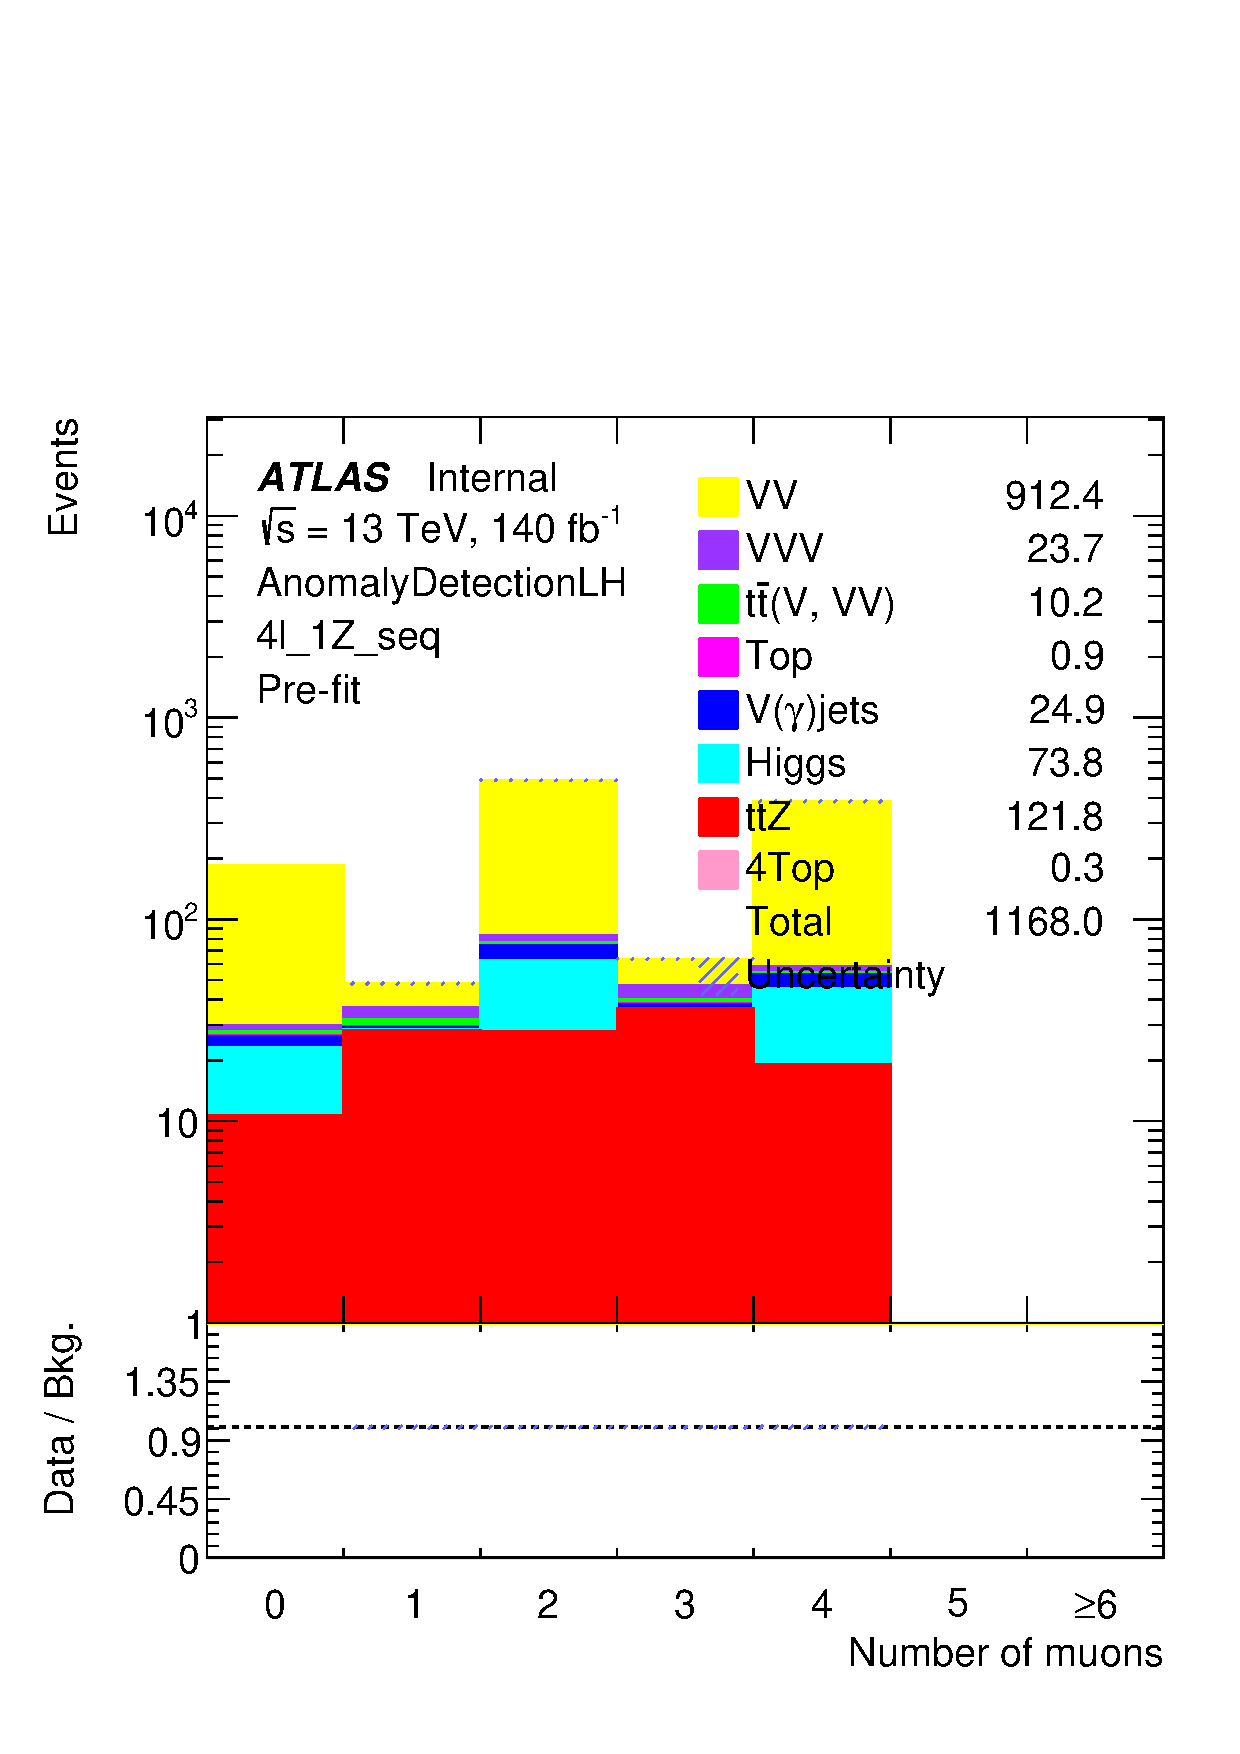
\includegraphics[width=0.24\textwidth]{plots/fourlepLH_run2/Plots/reg_4l_1Z_seq_nMuons.pdf} \\

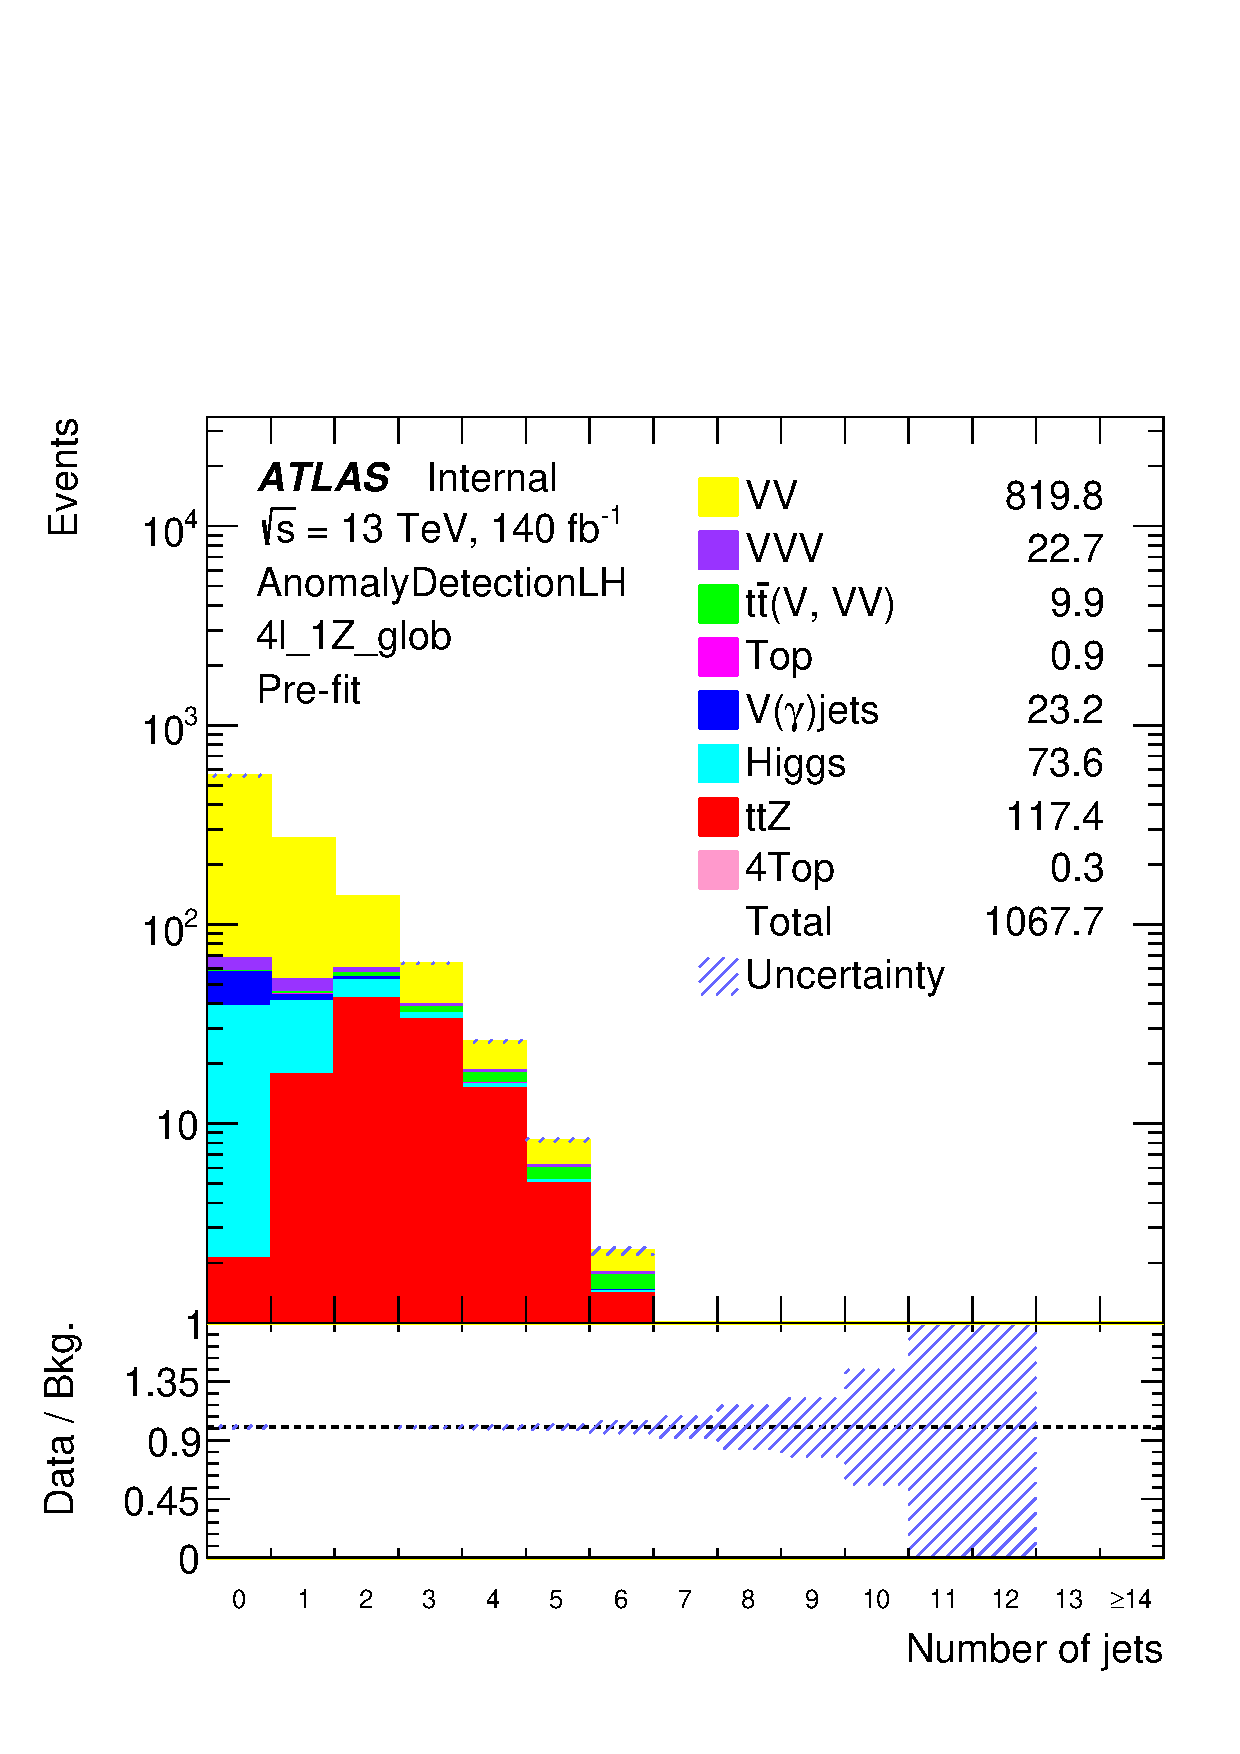
\includegraphics[width=0.24\textwidth]{plots/fourlepLH_run2/Plots/reg_4l_1Z_glob_nJets.pdf} &
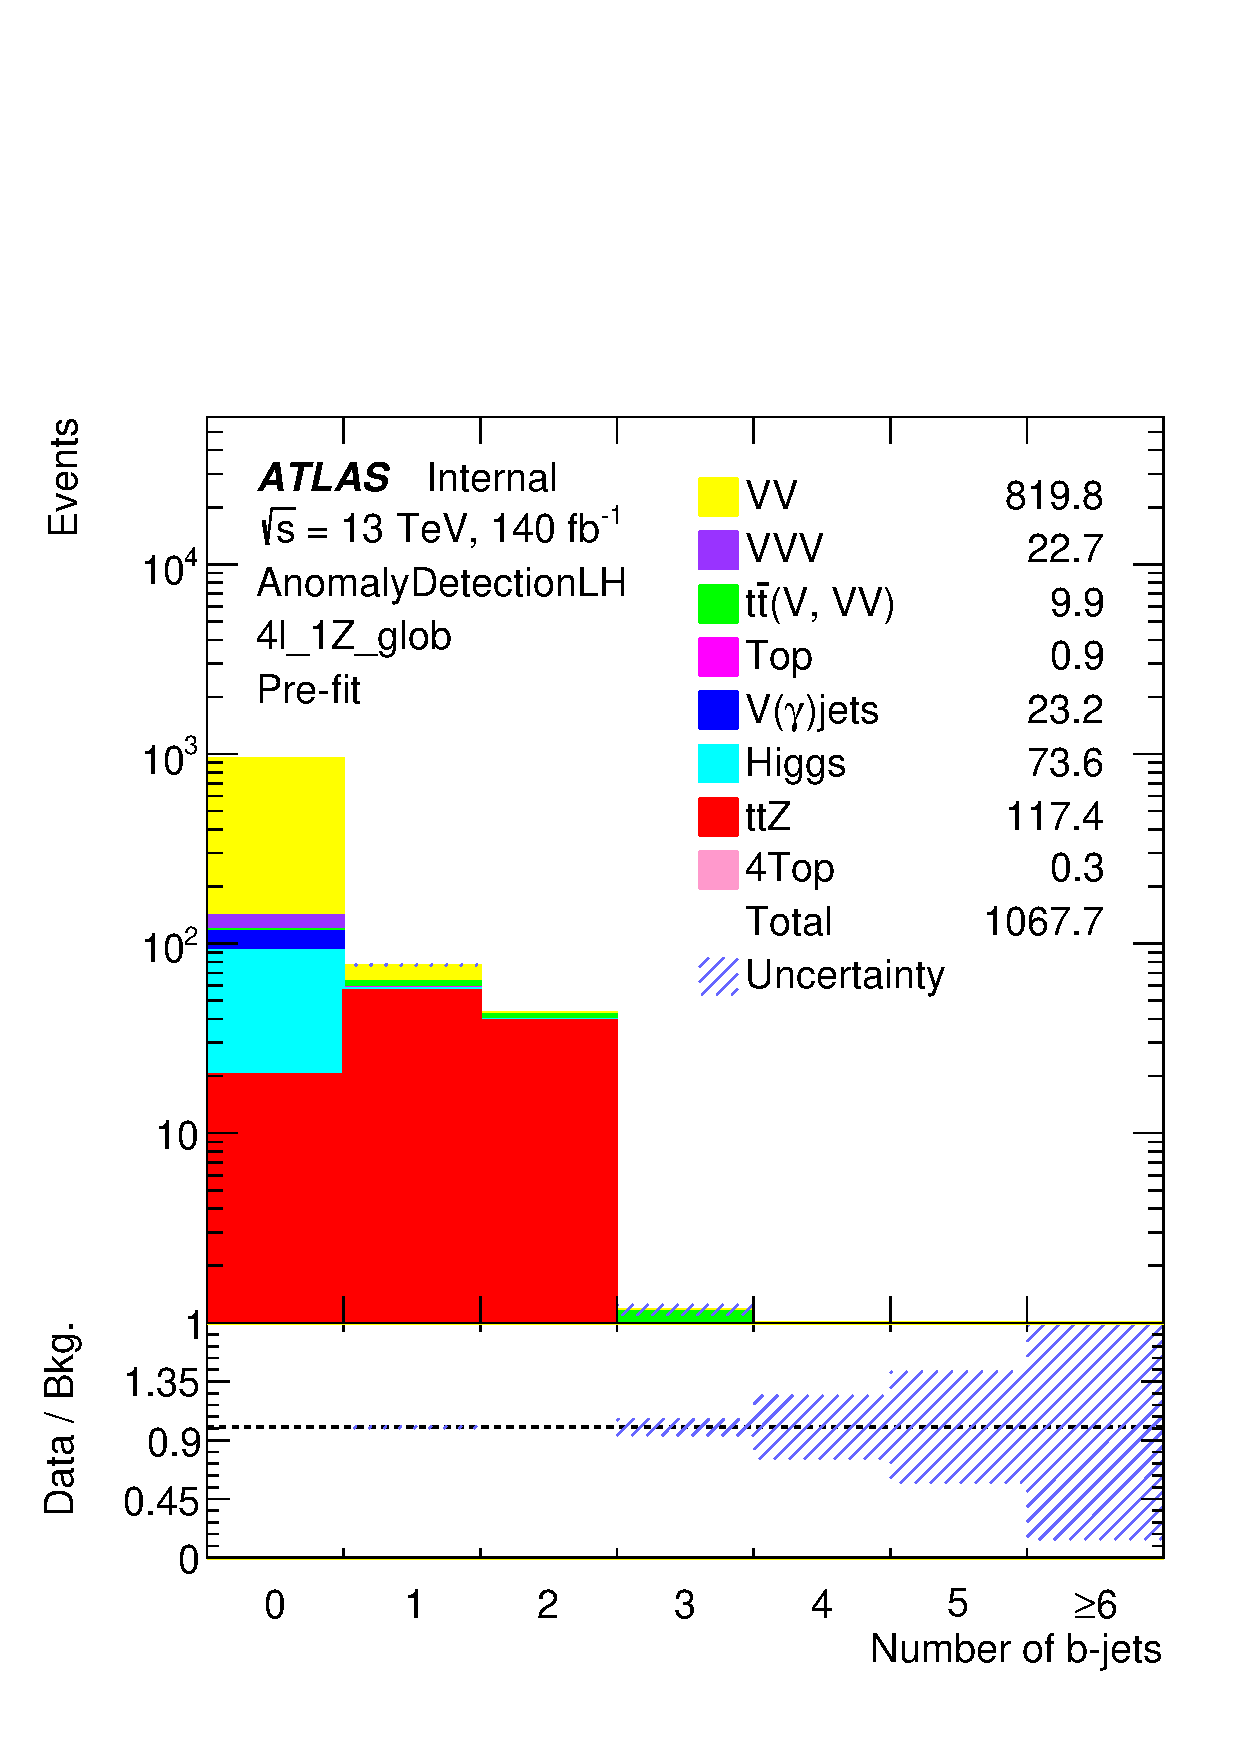
\includegraphics[width=0.24\textwidth]{plots/fourlepLH_run2/Plots/reg_4l_1Z_glob_nbJets.pdf} &
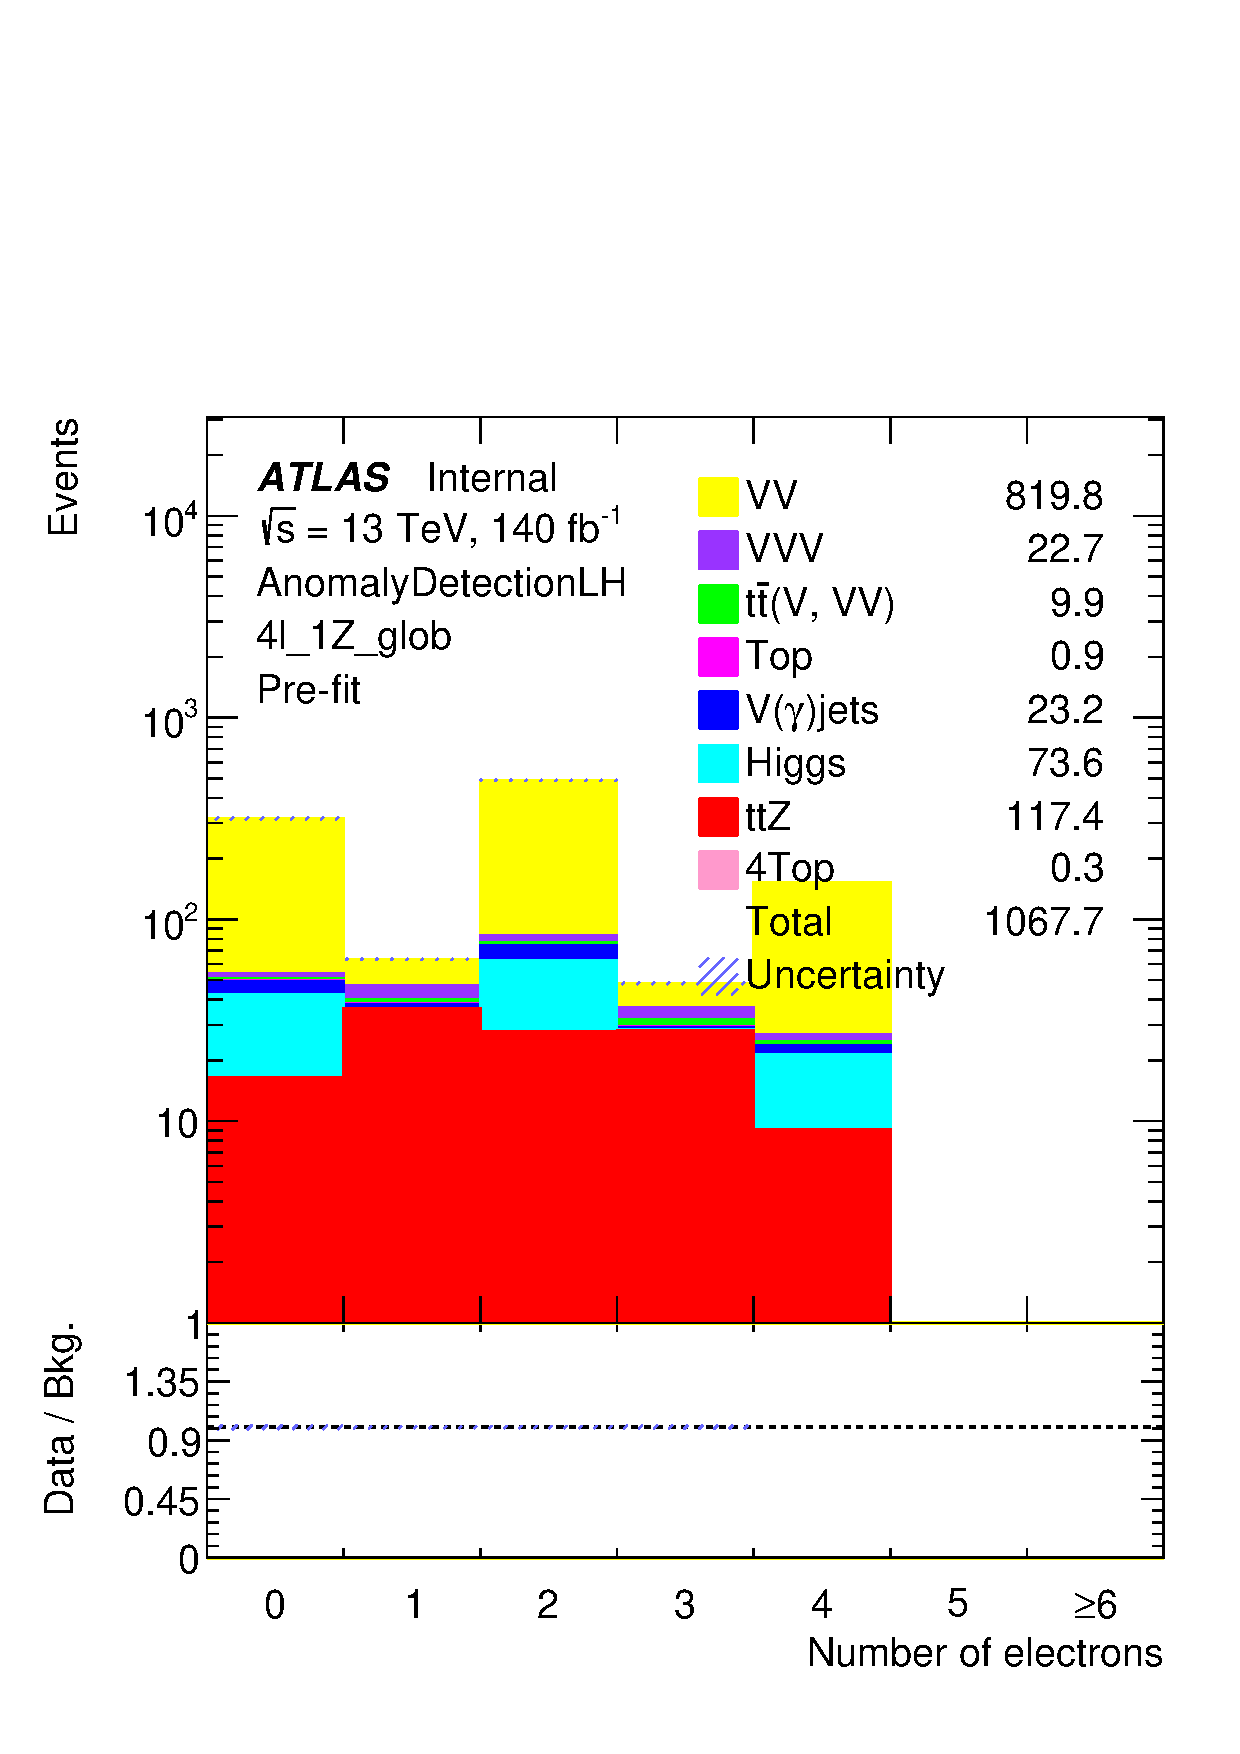
\includegraphics[width=0.24\textwidth]{plots/fourlepLH_run2/Plots/reg_4l_1Z_glob_nElectrons.pdf} &
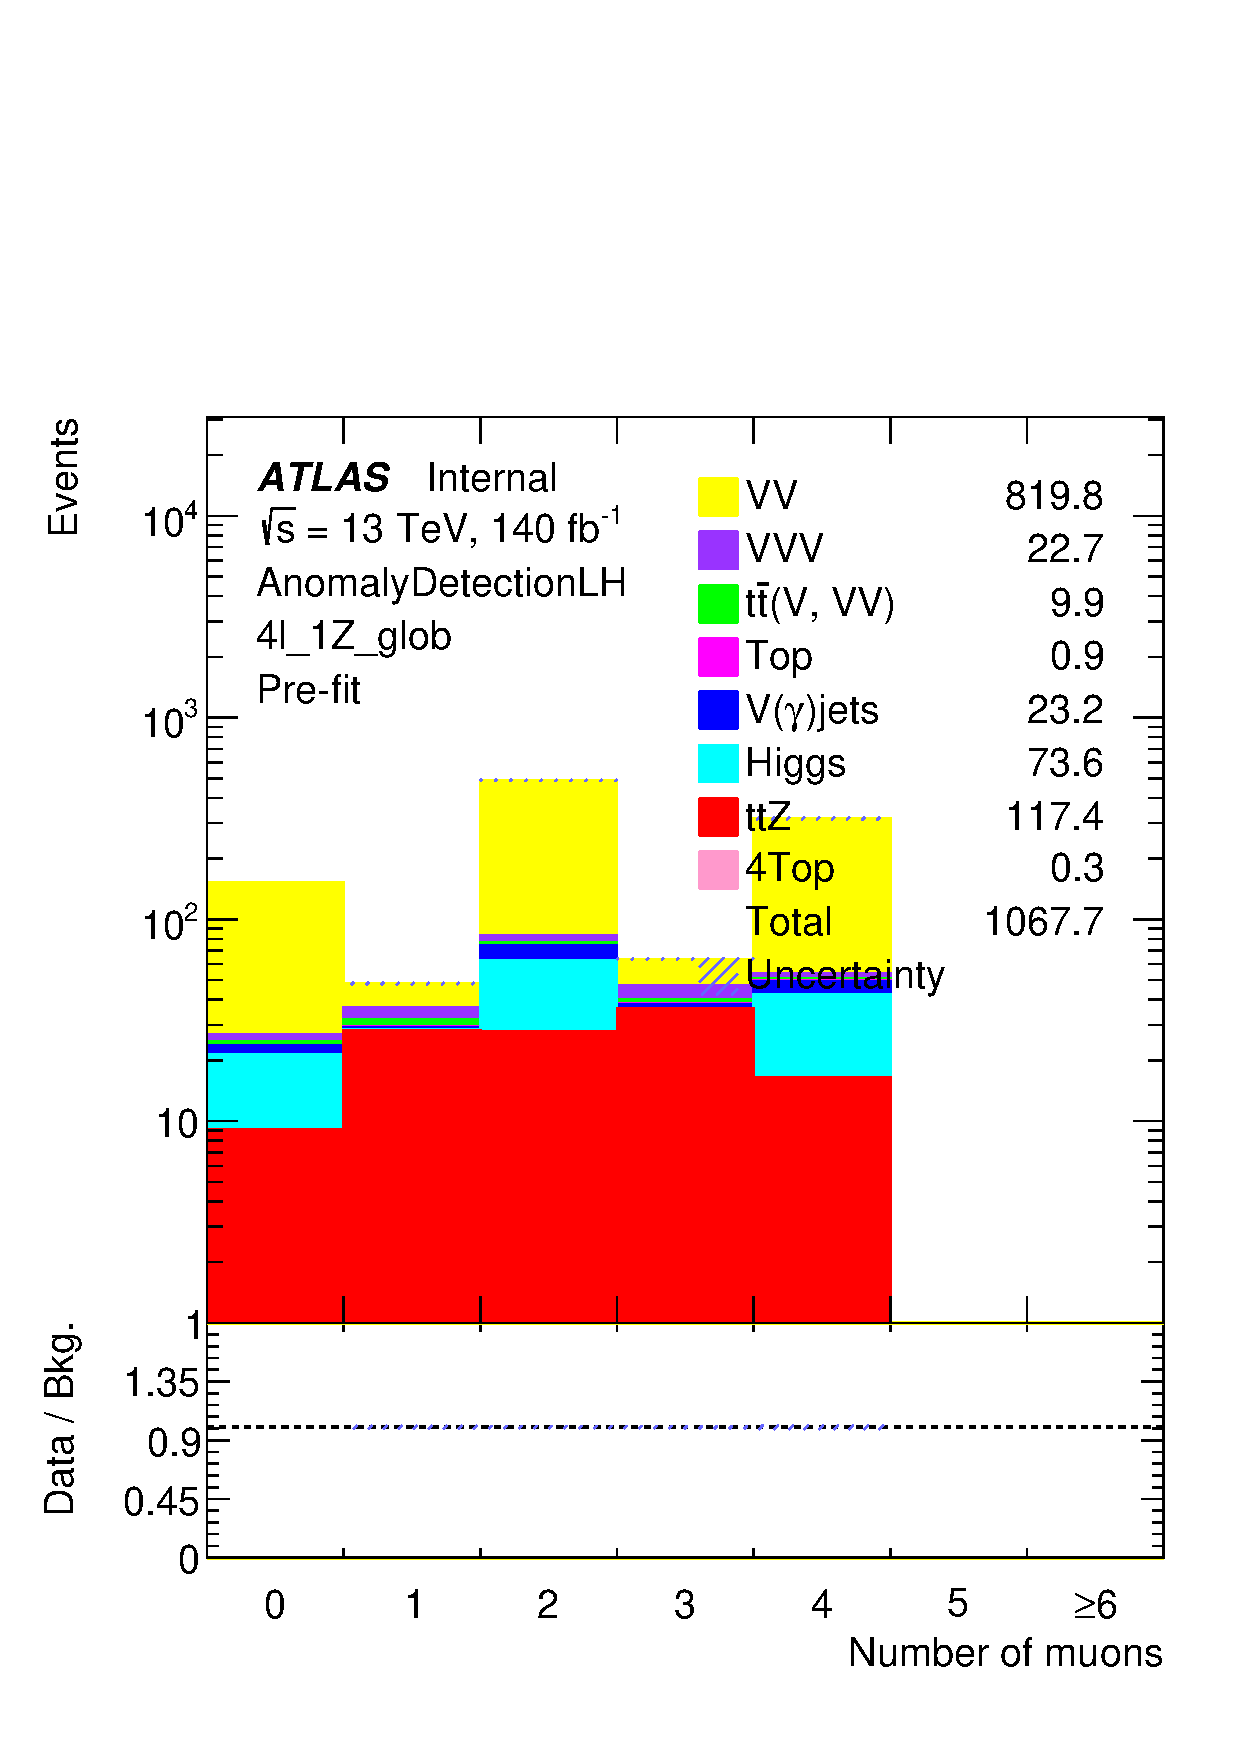
\includegraphics[width=0.24\textwidth]{plots/fourlepLH_run2/Plots/reg_4l_1Z_glob_nMuons.pdf} \\

\end{tabular}
\end{frame}

\begin{frame}{\texttt{Results: 4l\_1Z}}
\begin{tabular}{cccccc}
\includegraphics[width=0.24\textwidth]{plots/fourlepLH_run2/Plots/reg_4l_1Z_seq_lep_pt_0.pdf} &
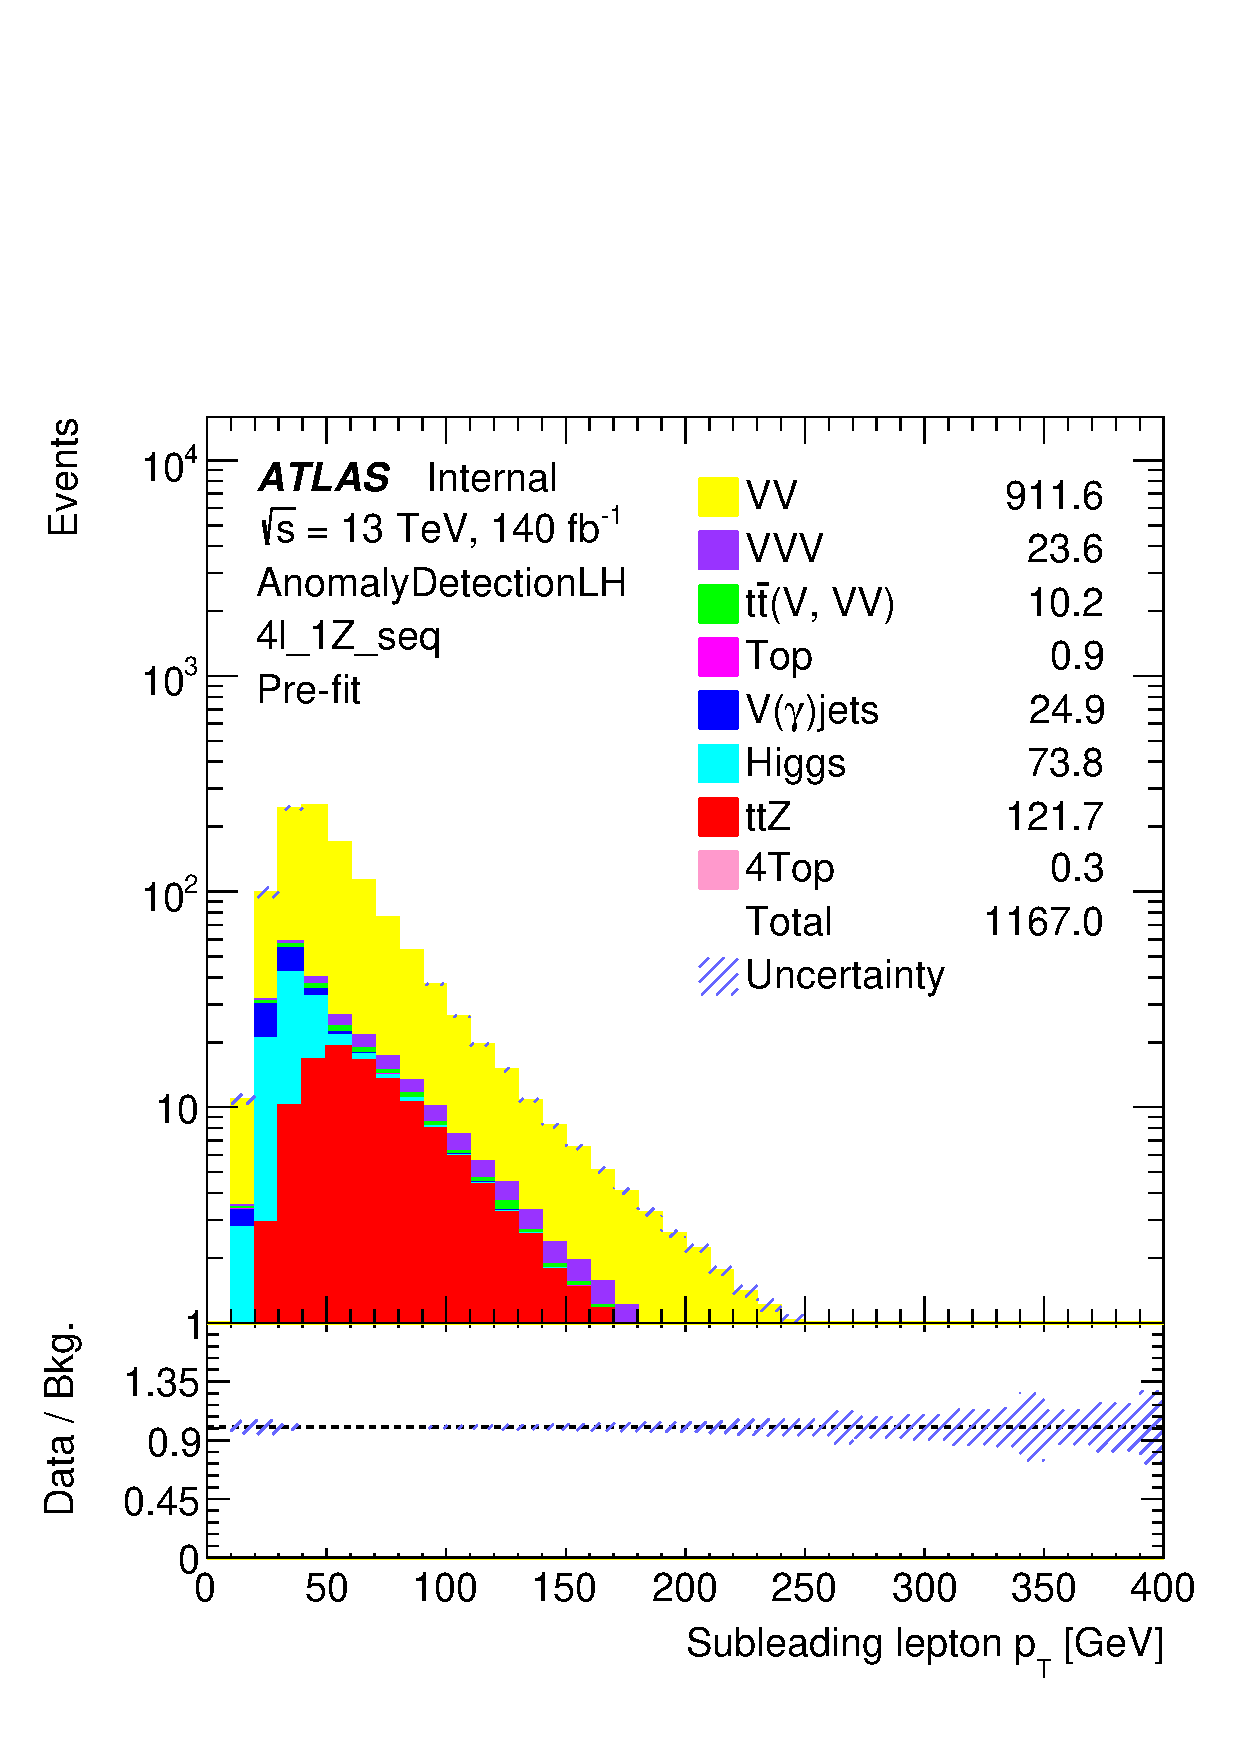
\includegraphics[width=0.24\textwidth]{plots/fourlepLH_run2/Plots/reg_4l_1Z_seq_lep_pt_1.pdf} &
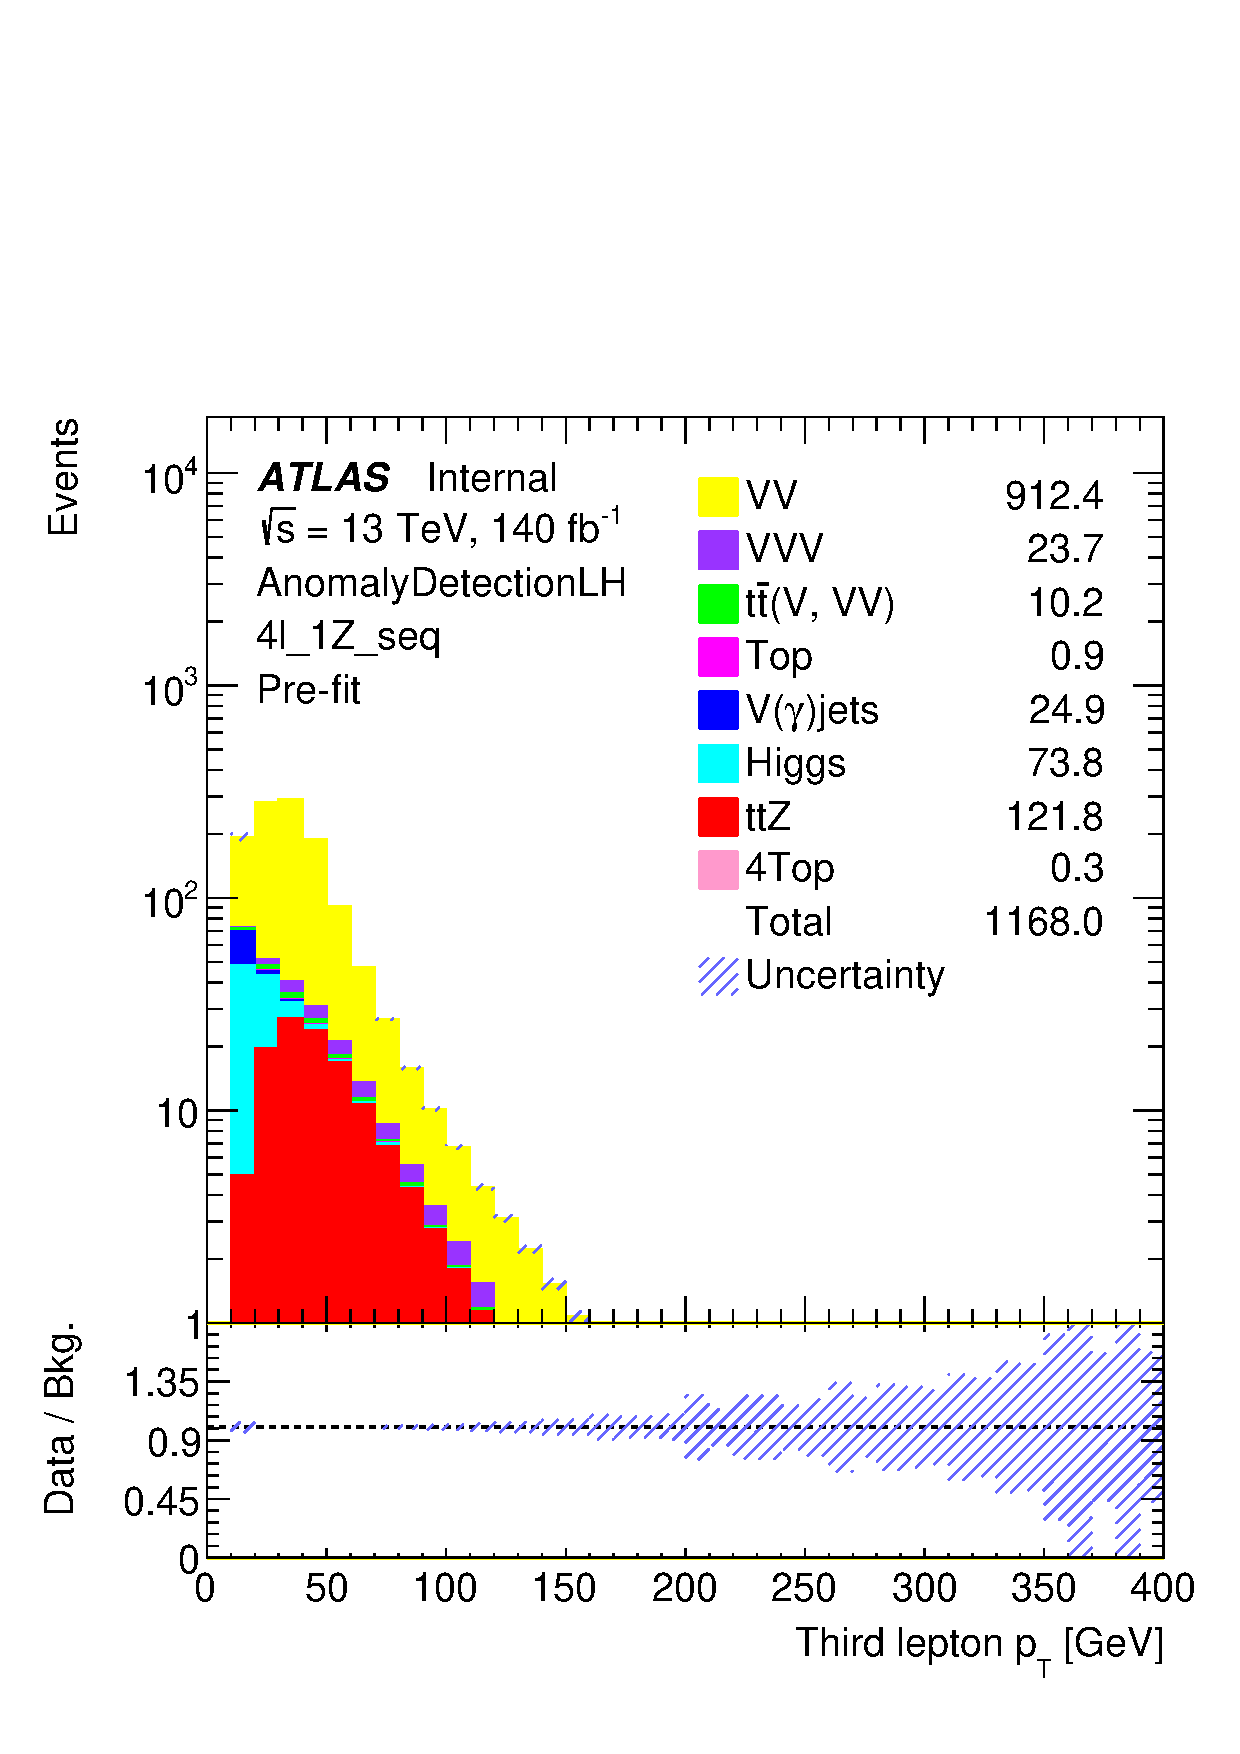
\includegraphics[width=0.24\textwidth]{plots/fourlepLH_run2/Plots/reg_4l_1Z_seq_lep_pt_2.pdf} &
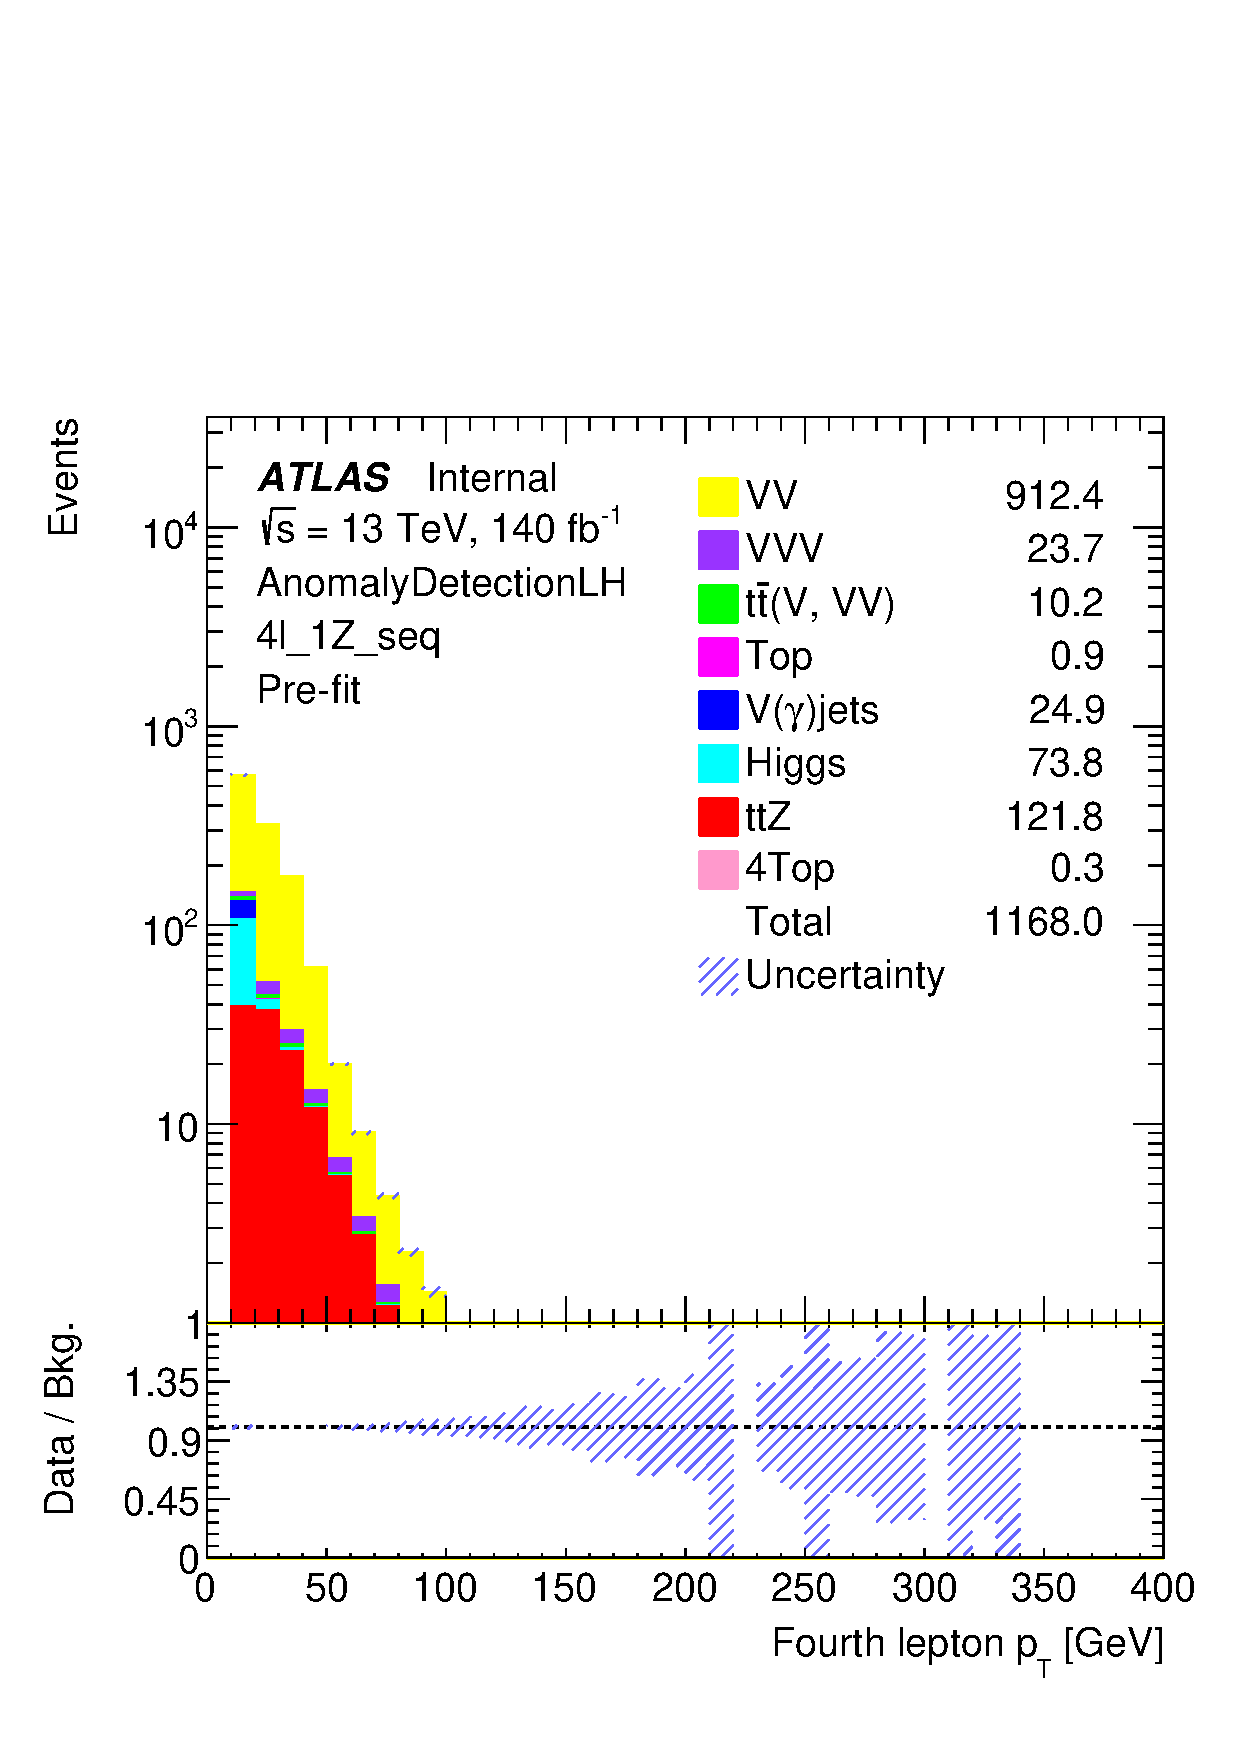
\includegraphics[width=0.24\textwidth]{plots/fourlepLH_run2/Plots/reg_4l_1Z_seq_lep_pt_3.pdf} \\

\includegraphics[width=0.24\textwidth]{plots/fourlepLH_run2/Plots/reg_4l_1Z_glob_lep_pt_0.pdf} &
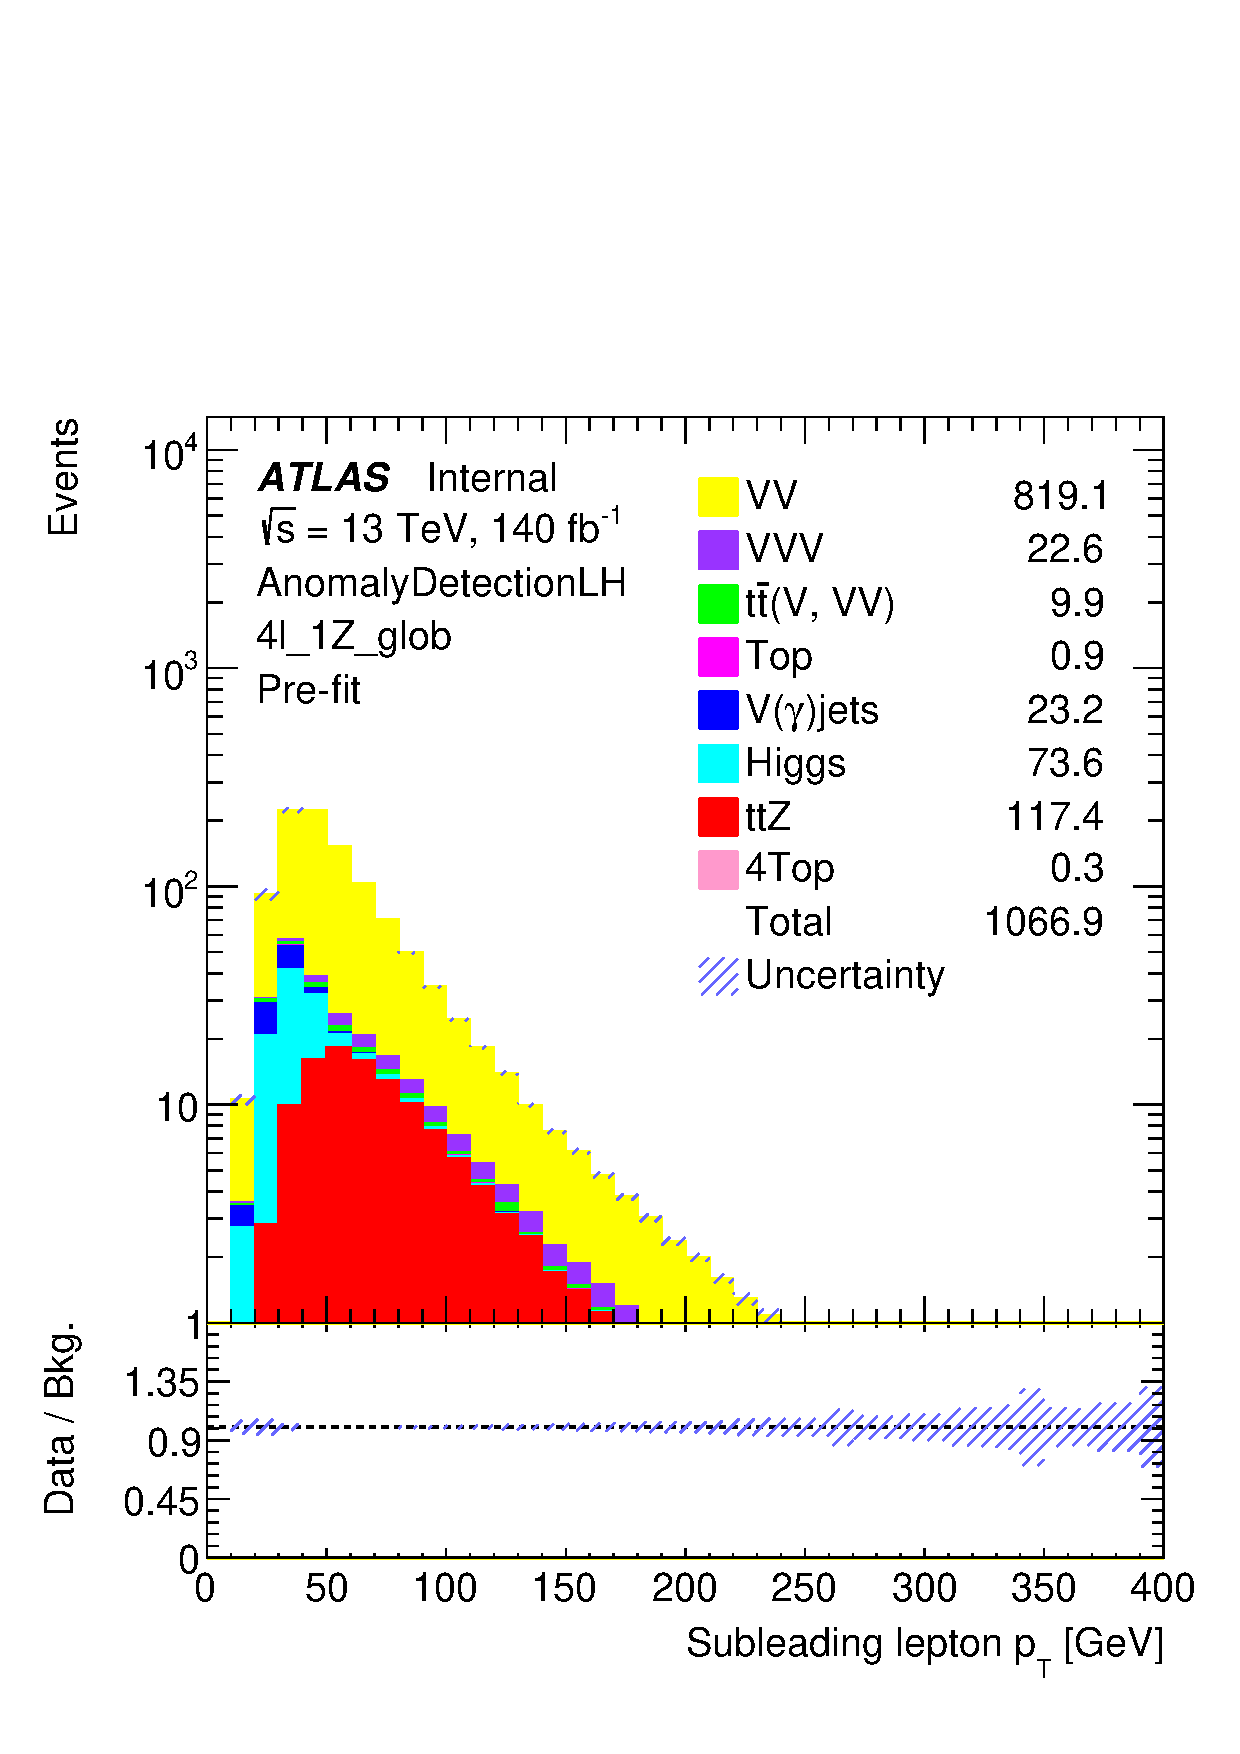
\includegraphics[width=0.24\textwidth]{plots/fourlepLH_run2/Plots/reg_4l_1Z_glob_lep_pt_1.pdf} &
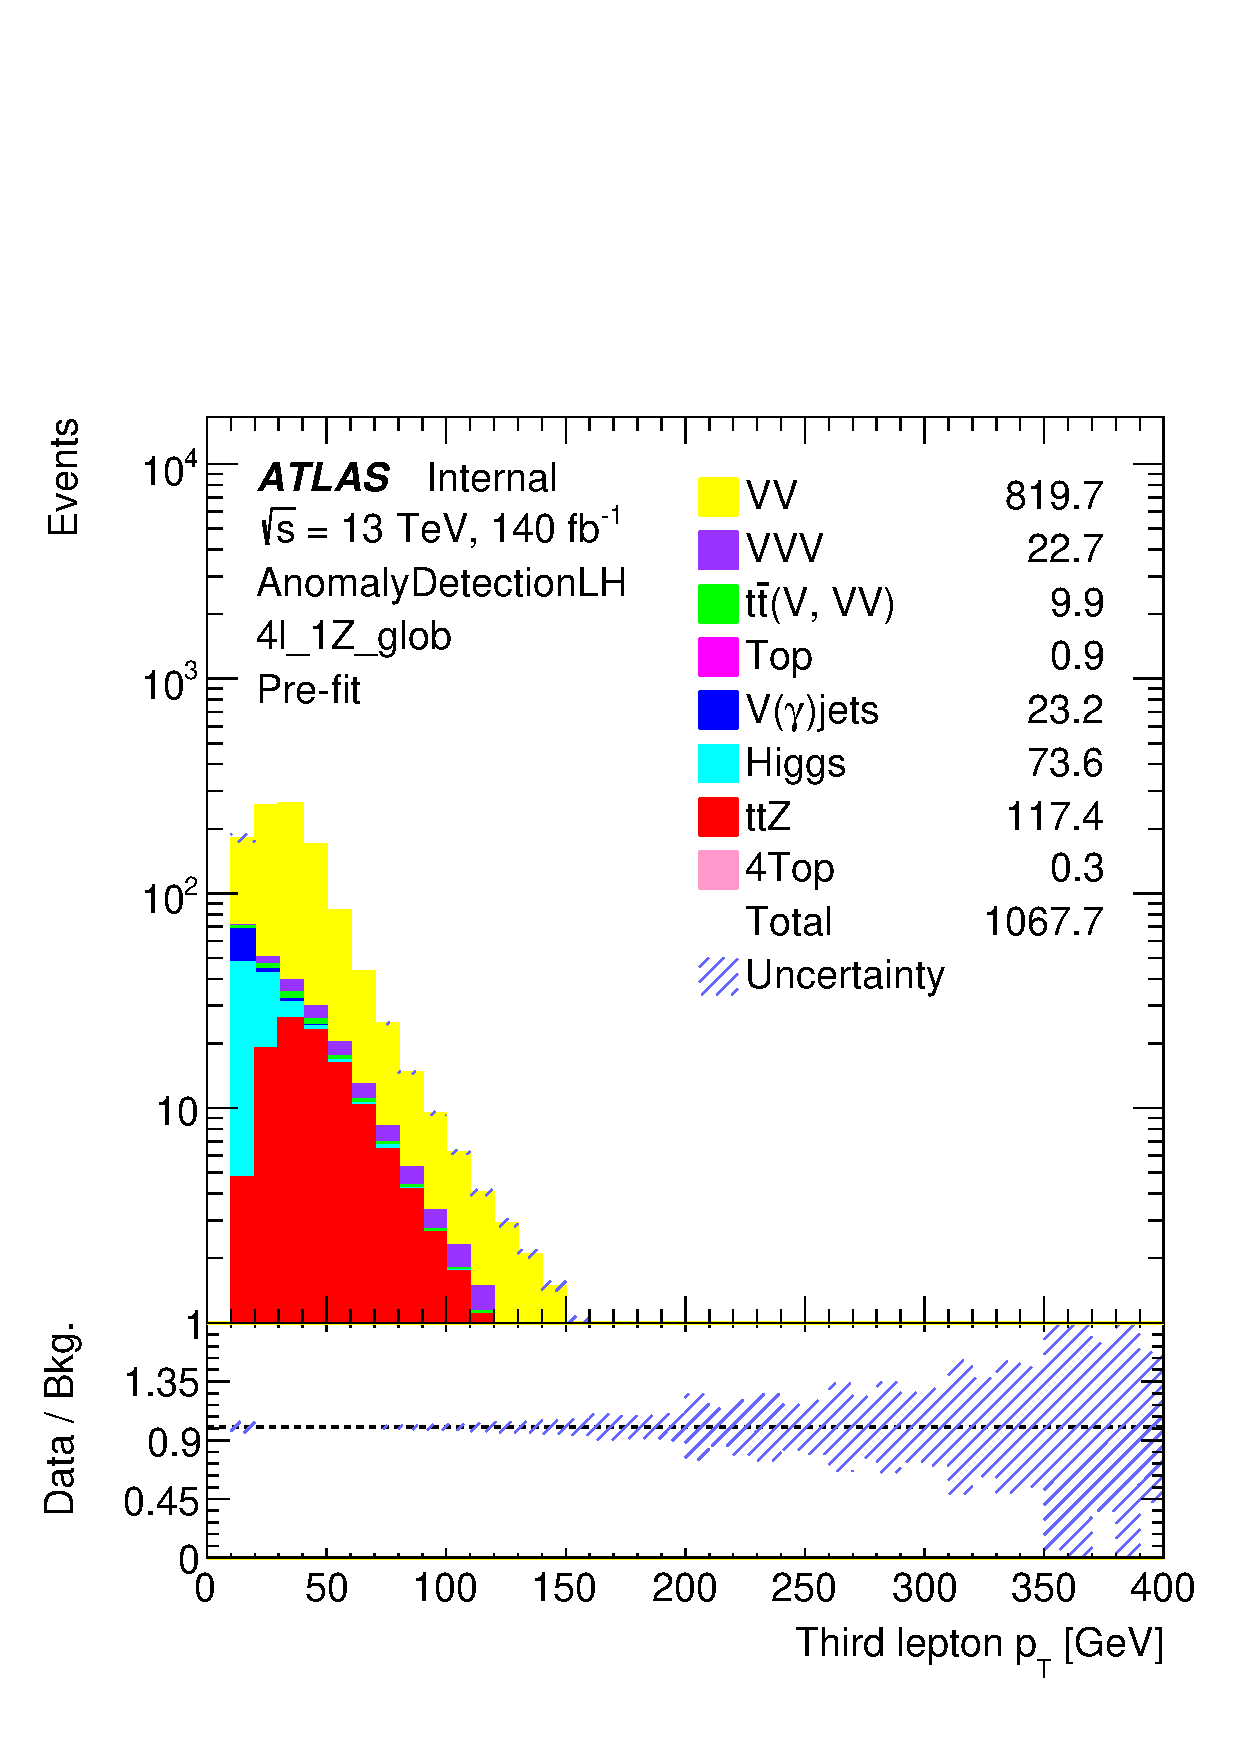
\includegraphics[width=0.24\textwidth]{plots/fourlepLH_run2/Plots/reg_4l_1Z_glob_lep_pt_2.pdf} &
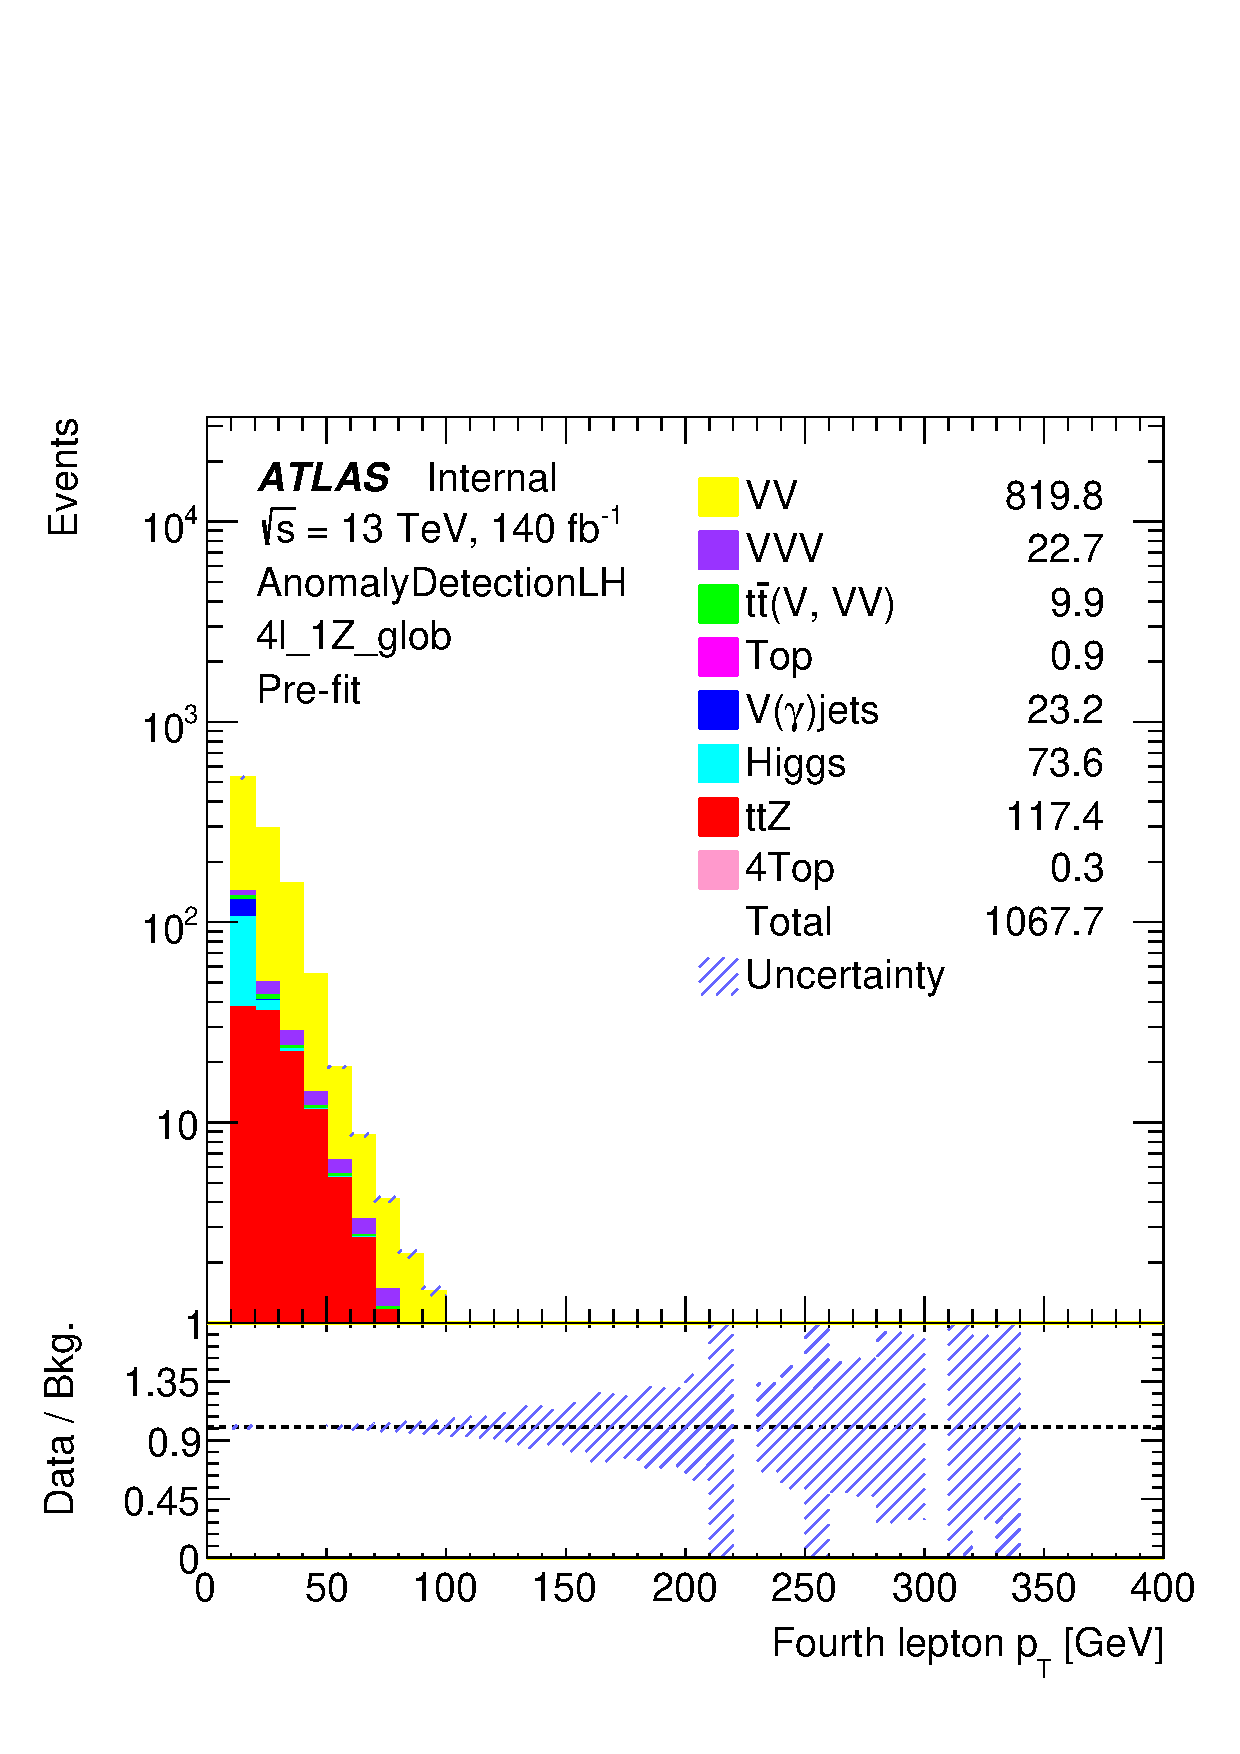
\includegraphics[width=0.24\textwidth]{plots/fourlepLH_run2/Plots/reg_4l_1Z_glob_lep_pt_3.pdf} \\

\end{tabular}

\end{frame}
\subsection{4l\_1Z\_0b}
\begin{frame}{\texttt{Focused selection: 4l\_1Z\_0b}}
%\tiny
\centering
\begin{tabular}{|c|c|}
\hline

4l\_1Z\_0b\_seq &
4l\_1Z\_0b\_glob \\
\hline
\multicolumn{2}{|c|}{\texttt{globalTriggerMatchSLTorDLT\_LooseLH\_custTrig\_NOSYS}} \\
\multicolumn{2}{|c|}{\texttt{pass\_fourlep\_LooseLH\_NOSYS} }\\
\multicolumn{2}{|c|}{\texttt{$N_{leptons}$=4}} \\
\multicolumn{2}{|c|}{\texttt{$N_{taus}$ $\geq 0$} } \\
\multicolumn{2}{|c|}{$N_{b\mathrm{-jets}}$ $= 0$} \\
\multicolumn{2}{|c|}{\texttt{Q = 0}} \\

\hline

\texttt{$|m_{Z1}^{seq}-91.2e3| < 10e3$} &
\texttt{$|m_{Z1}^{glob}-91.2e3| < 10e3$} &\\
\texttt{$|m_{Z2}^{seq}-91.2e3| < 10e3$} &
\texttt{$|m_{Z2}^{glob}-91.2e3| < 10e3$}\\

\hline

\end{tabular}
\end{frame}

\begin{frame}{\texttt{Results: 4l\_1Z\_0b}}
\centering
\begin{tabular}{cccccc}

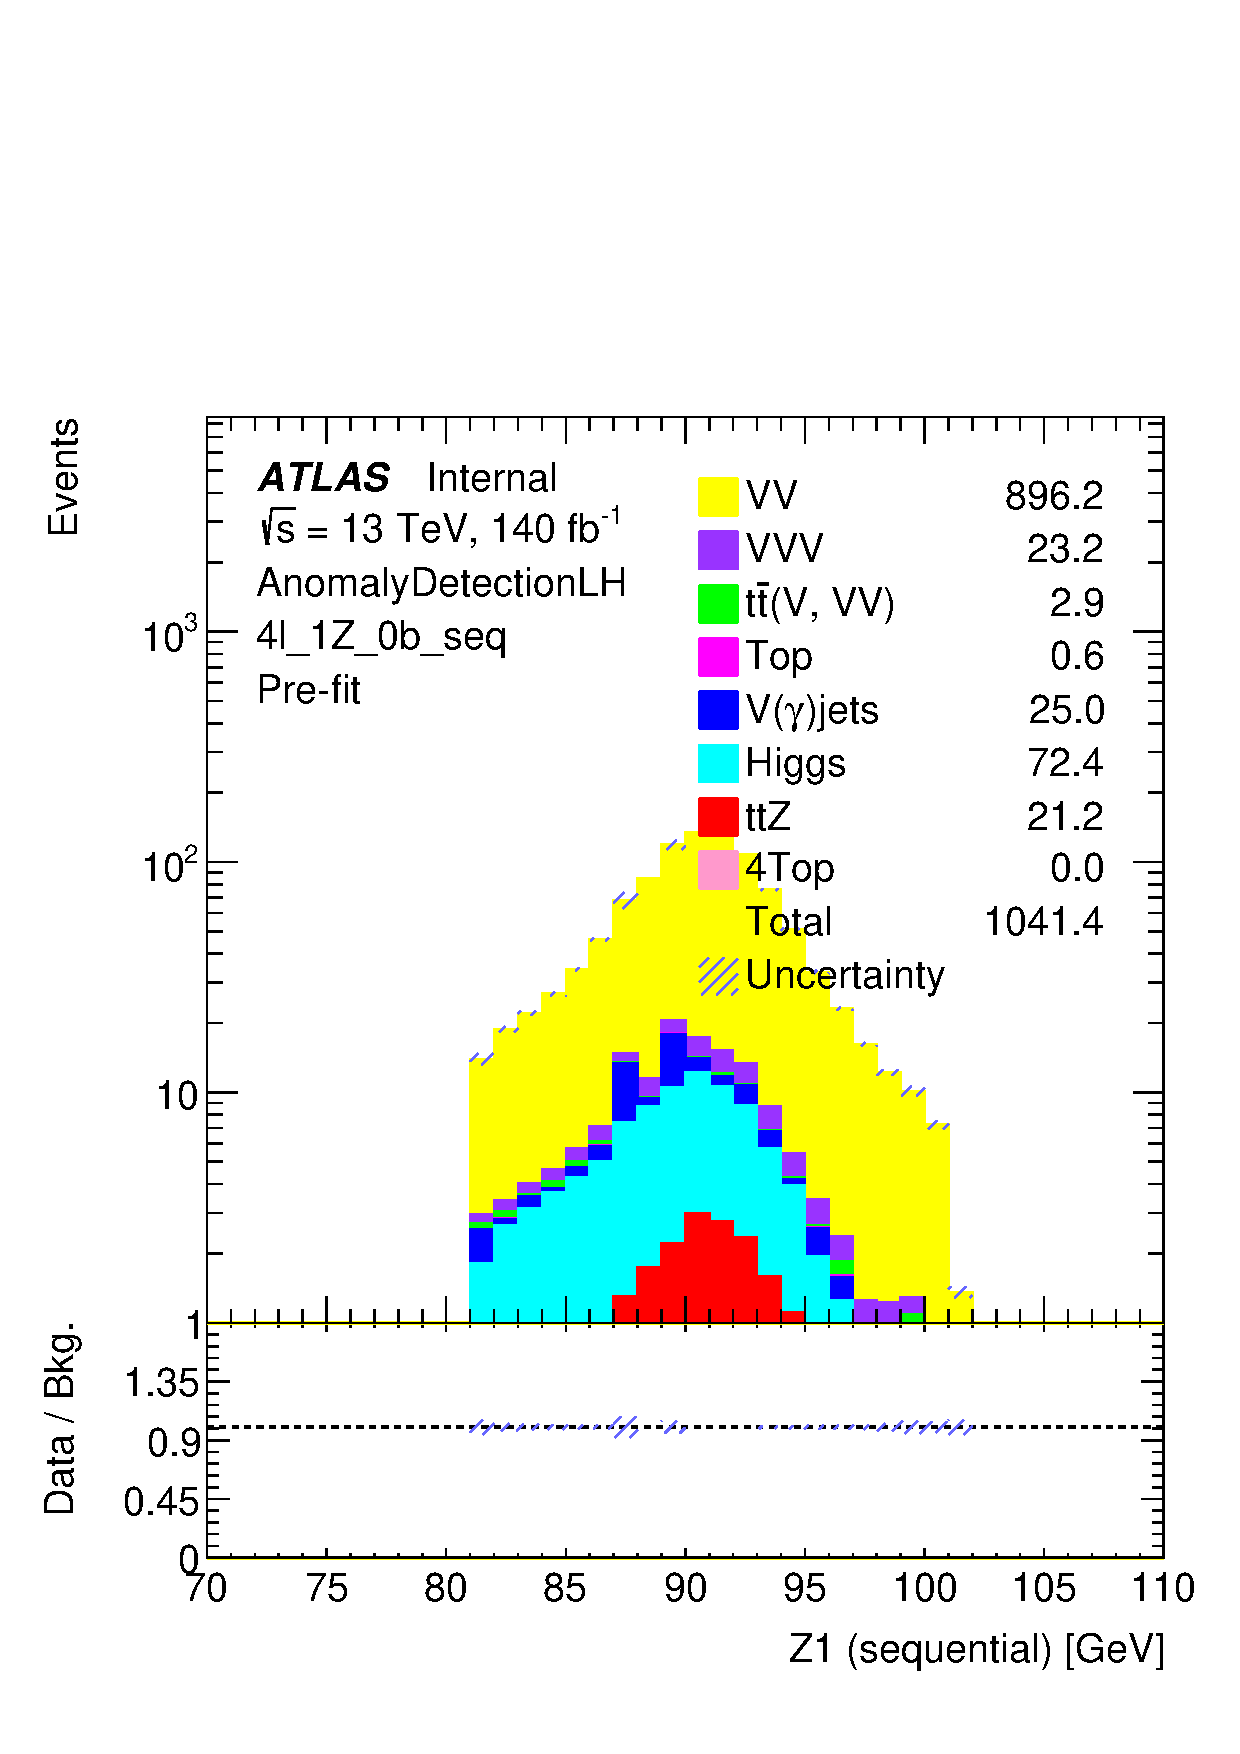
\includegraphics[width=0.24\textwidth]{plots/fourlepLH_run2/Plots/reg_4l_1Z_0b_seq_Z1_mass_seq_1GeV.pdf} &
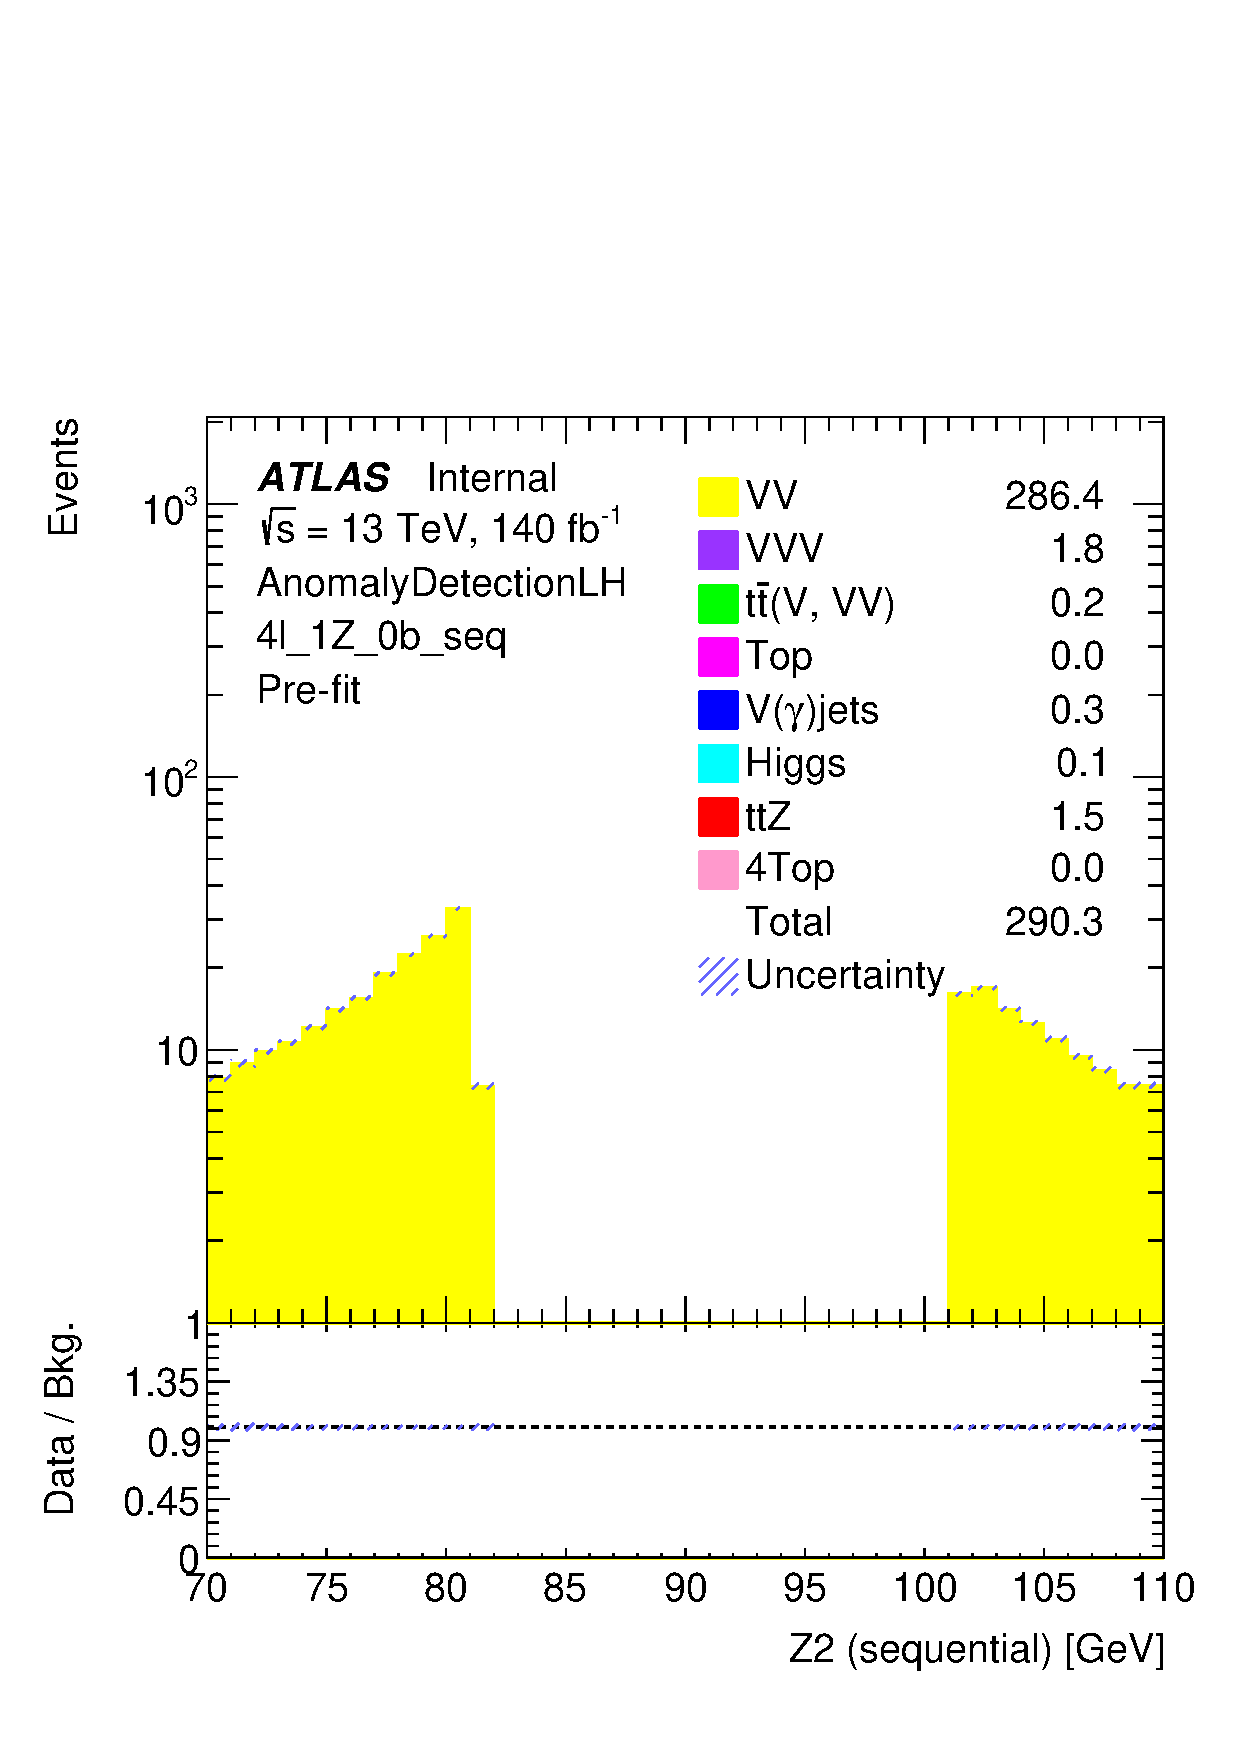
\includegraphics[width=0.24\textwidth]{plots/fourlepLH_run2/Plots/reg_4l_1Z_0b_seq_Z2_mass_seq_1GeV.pdf}  &

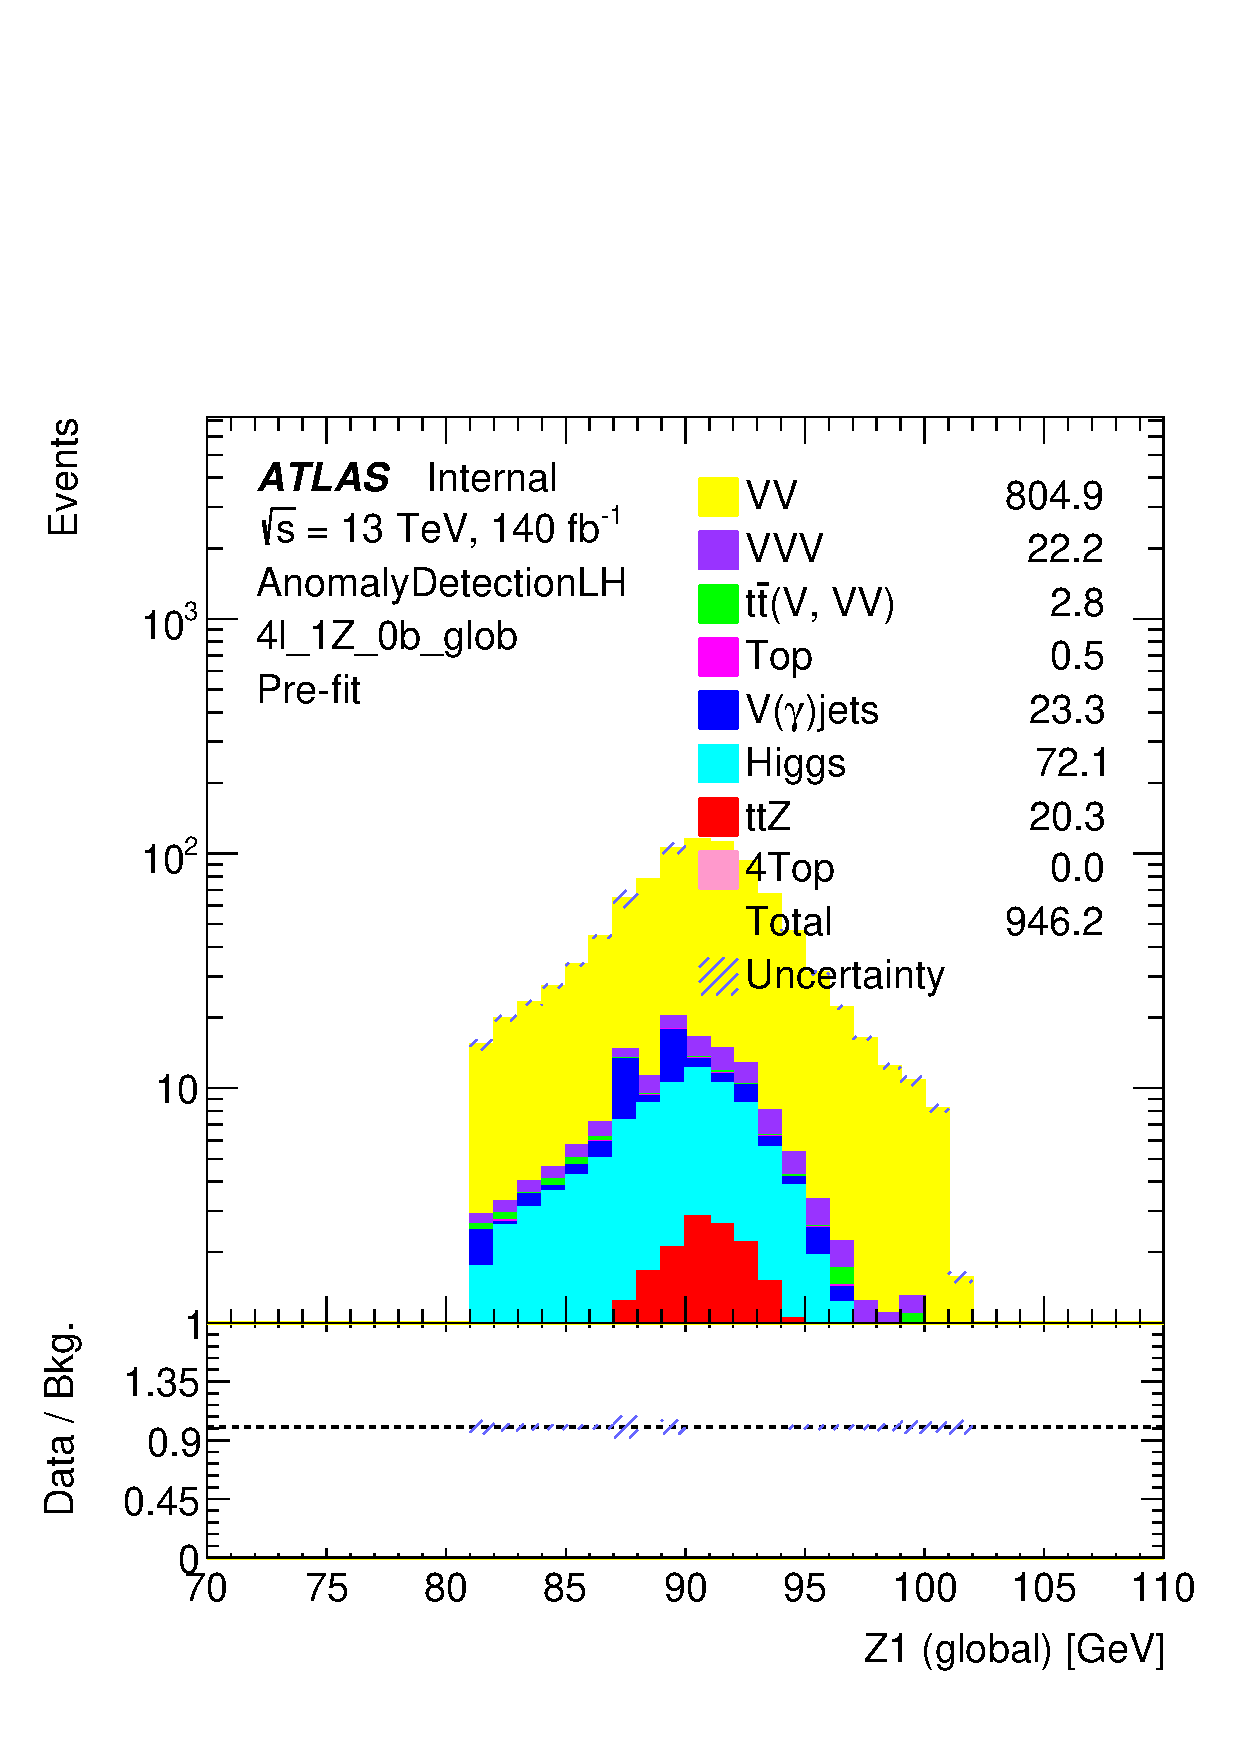
\includegraphics[width=0.24\textwidth]{plots/fourlepLH_run2/Plots/reg_4l_1Z_0b_glob_Z1_mass_glob_1GeV.pdf} &
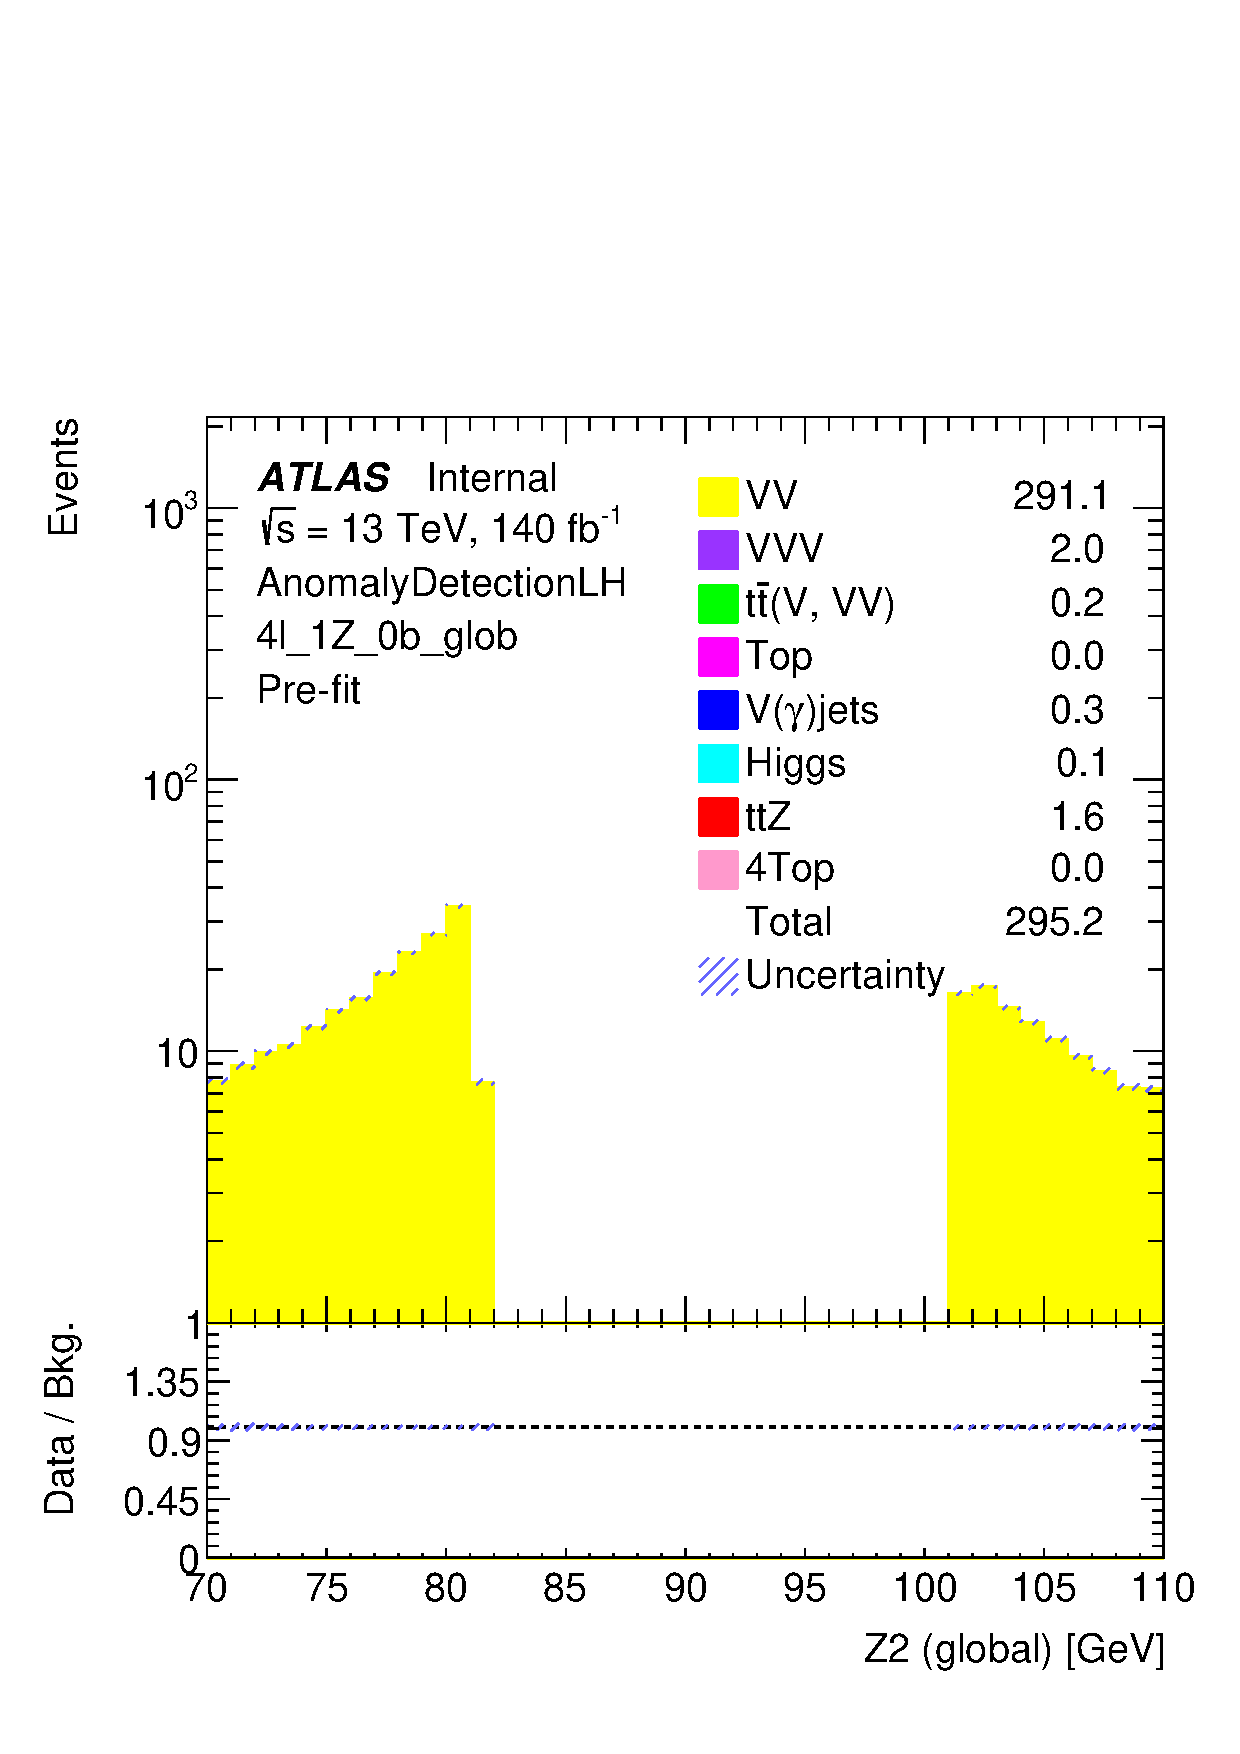
\includegraphics[width=0.24\textwidth]{plots/fourlepLH_run2/Plots/reg_4l_1Z_0b_glob_Z2_mass_glob_1GeV.pdf}\\

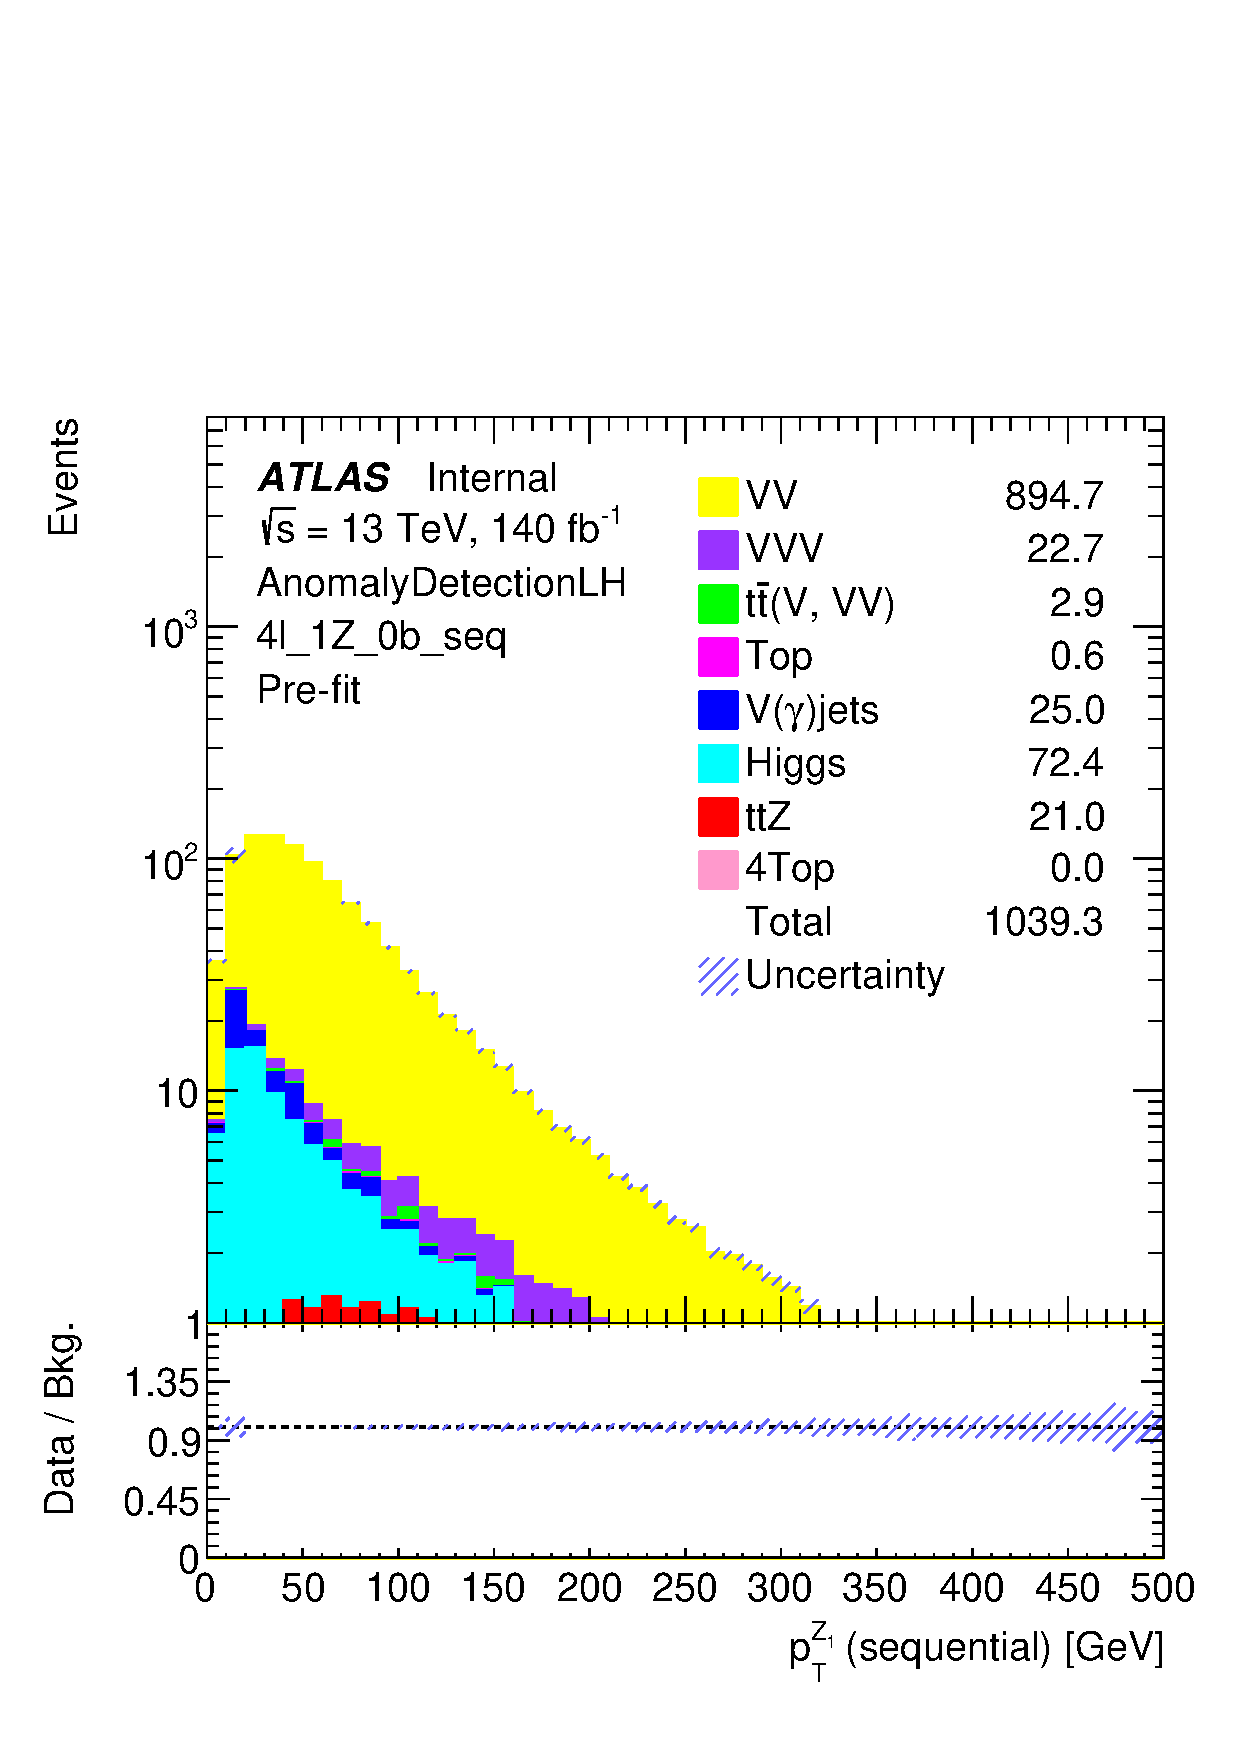
\includegraphics[width=0.24\textwidth]{plots/fourlepLH_run2/Plots/reg_4l_1Z_0b_seq_Z1_pt_seq.pdf} &
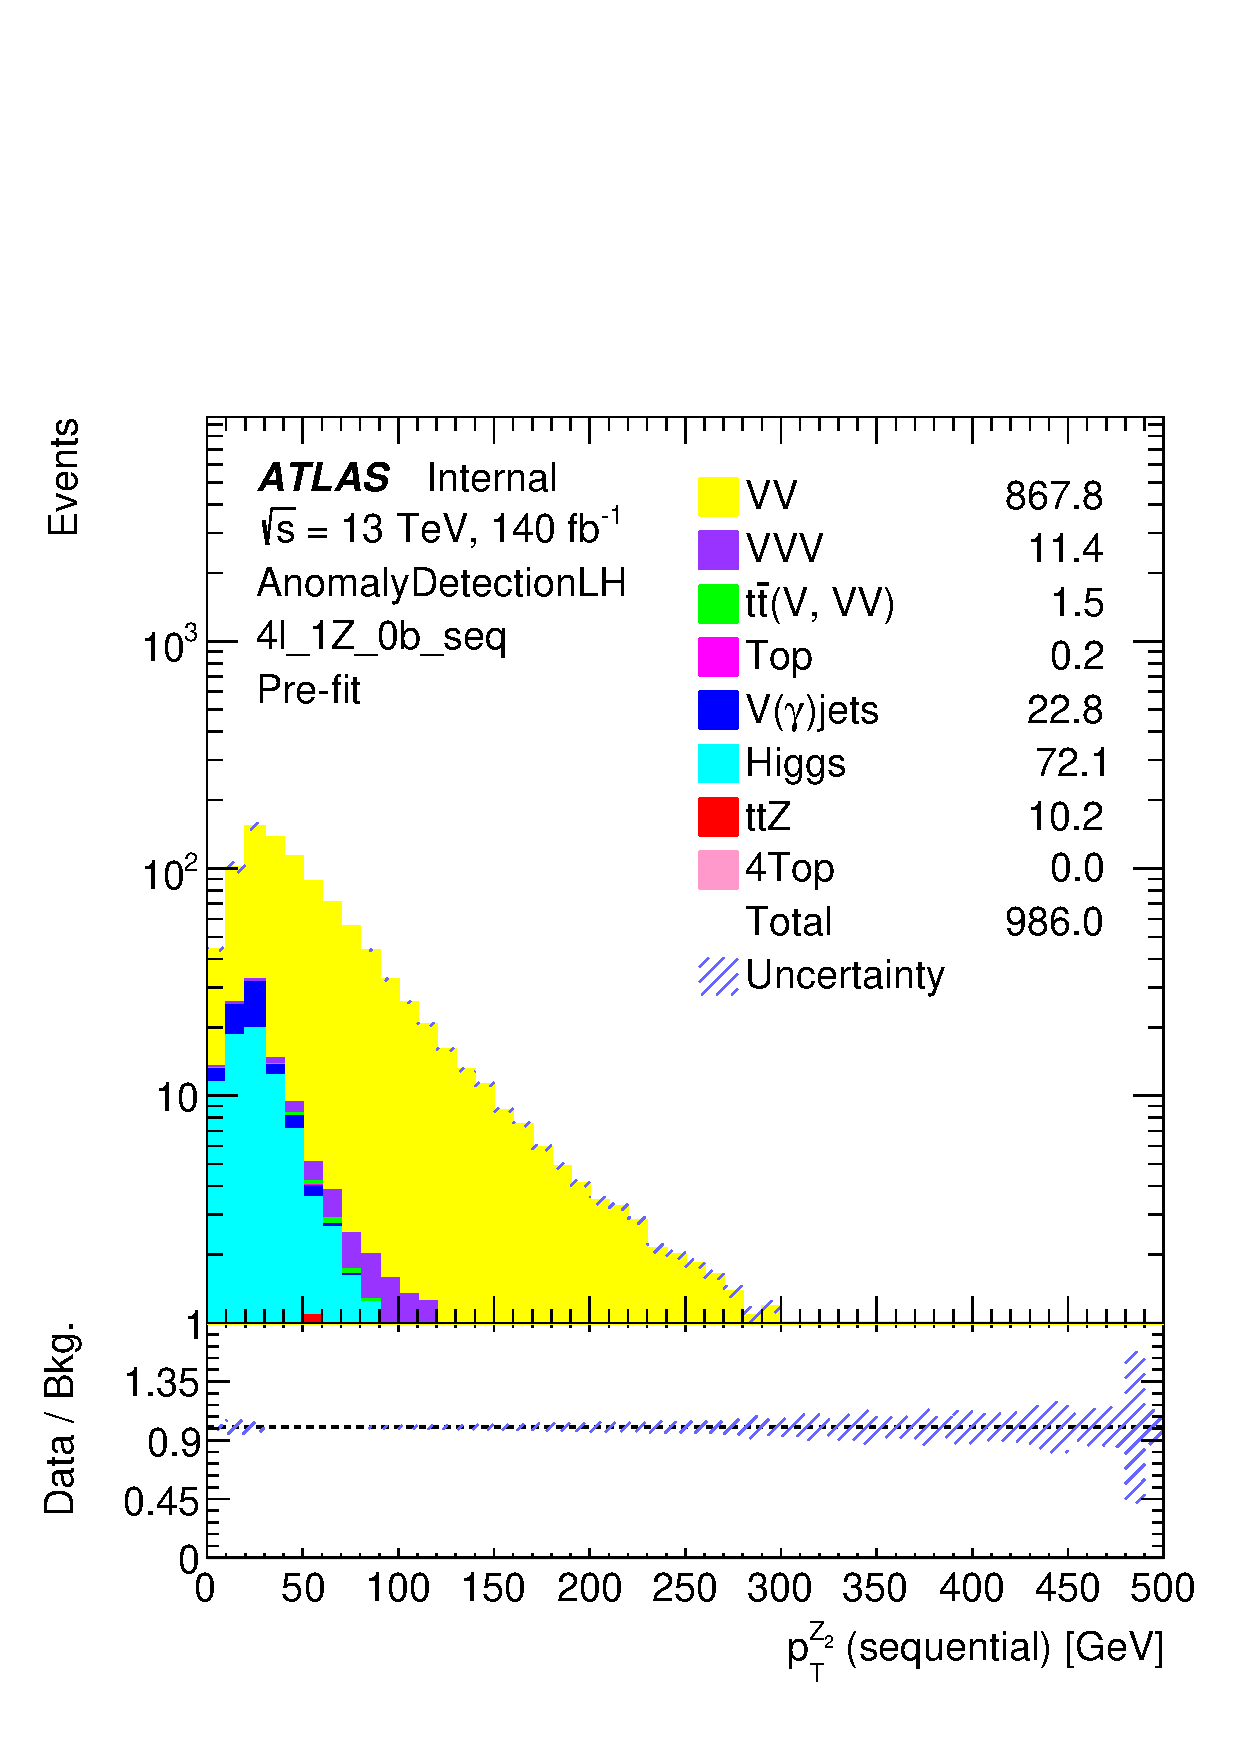
\includegraphics[width=0.24\textwidth]{plots/fourlepLH_run2/Plots/reg_4l_1Z_0b_seq_Z2_pt_seq.pdf}  &

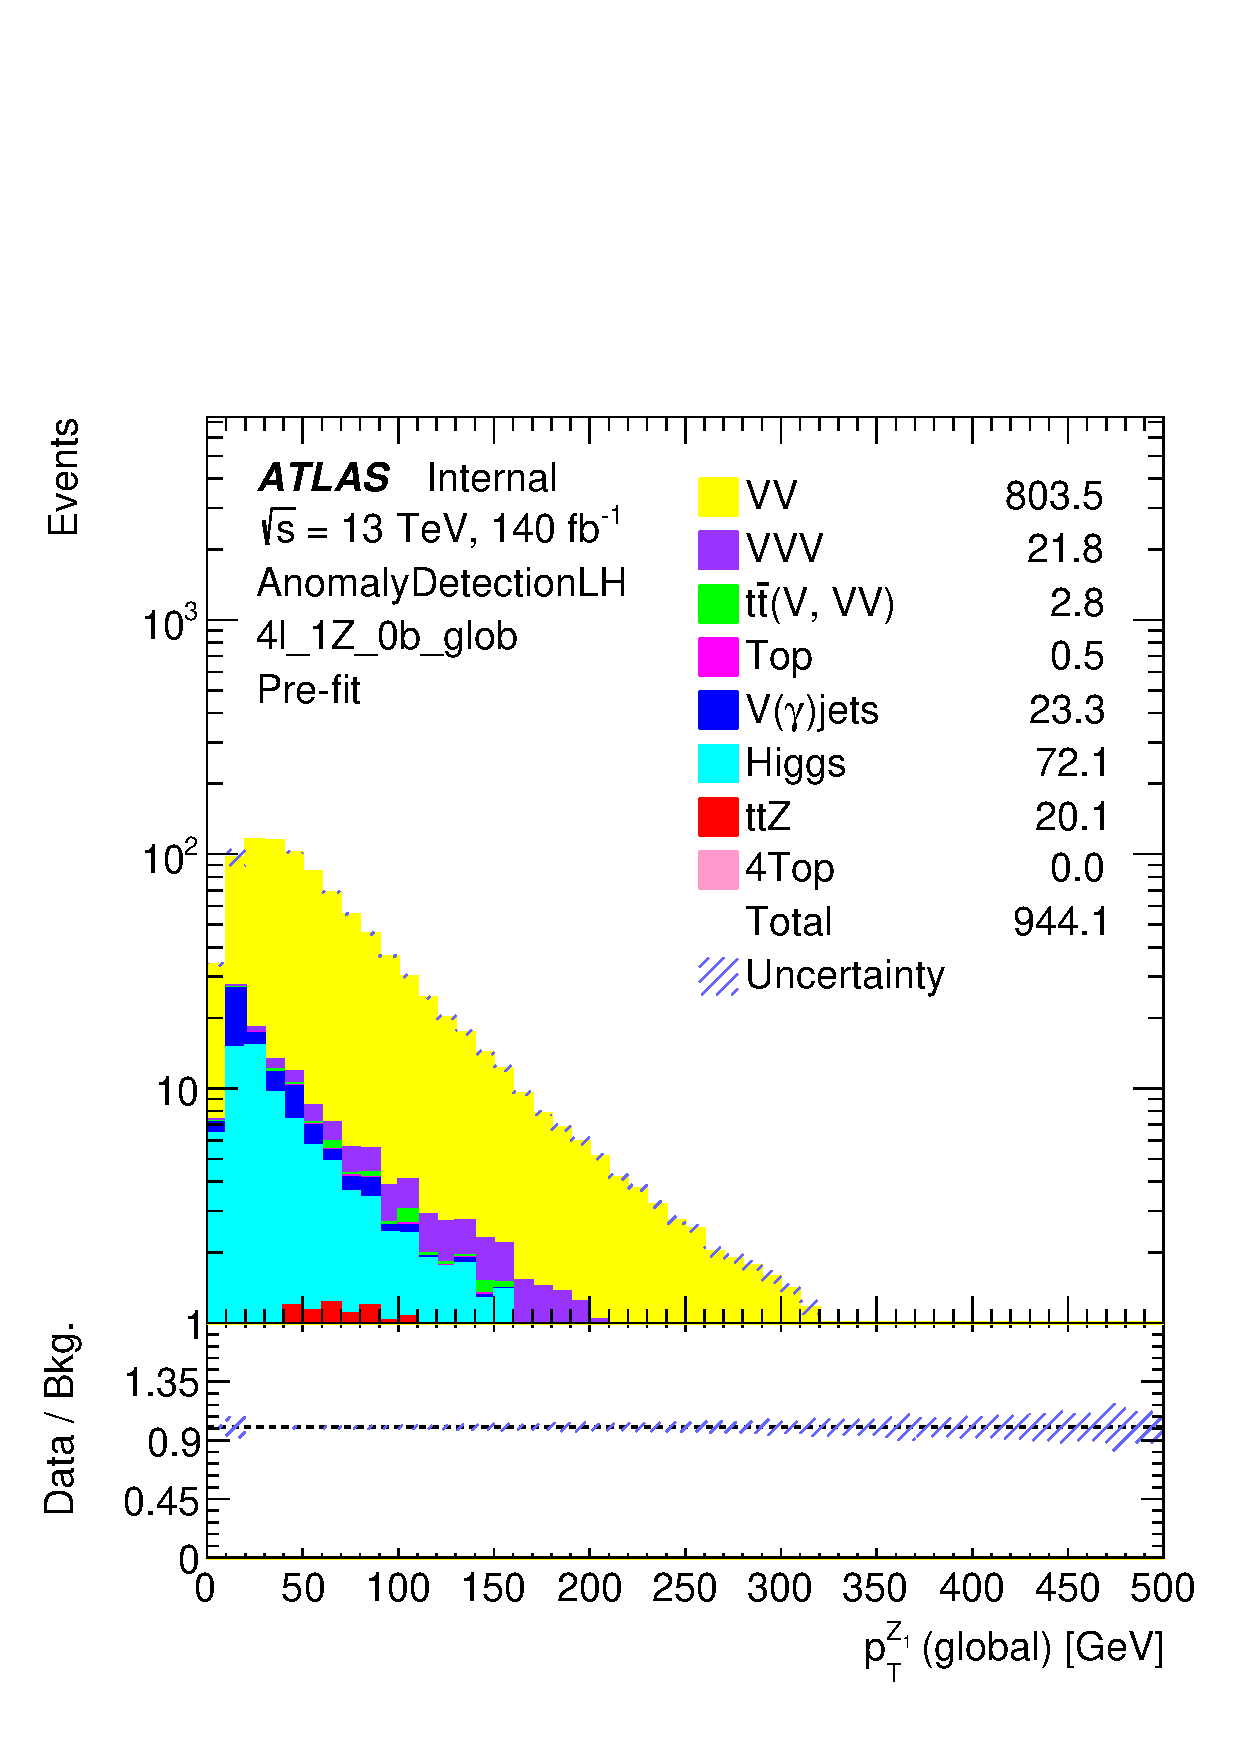
\includegraphics[width=0.24\textwidth]{plots/fourlepLH_run2/Plots/reg_4l_1Z_0b_glob_Z1_pt_glob.pdf} &
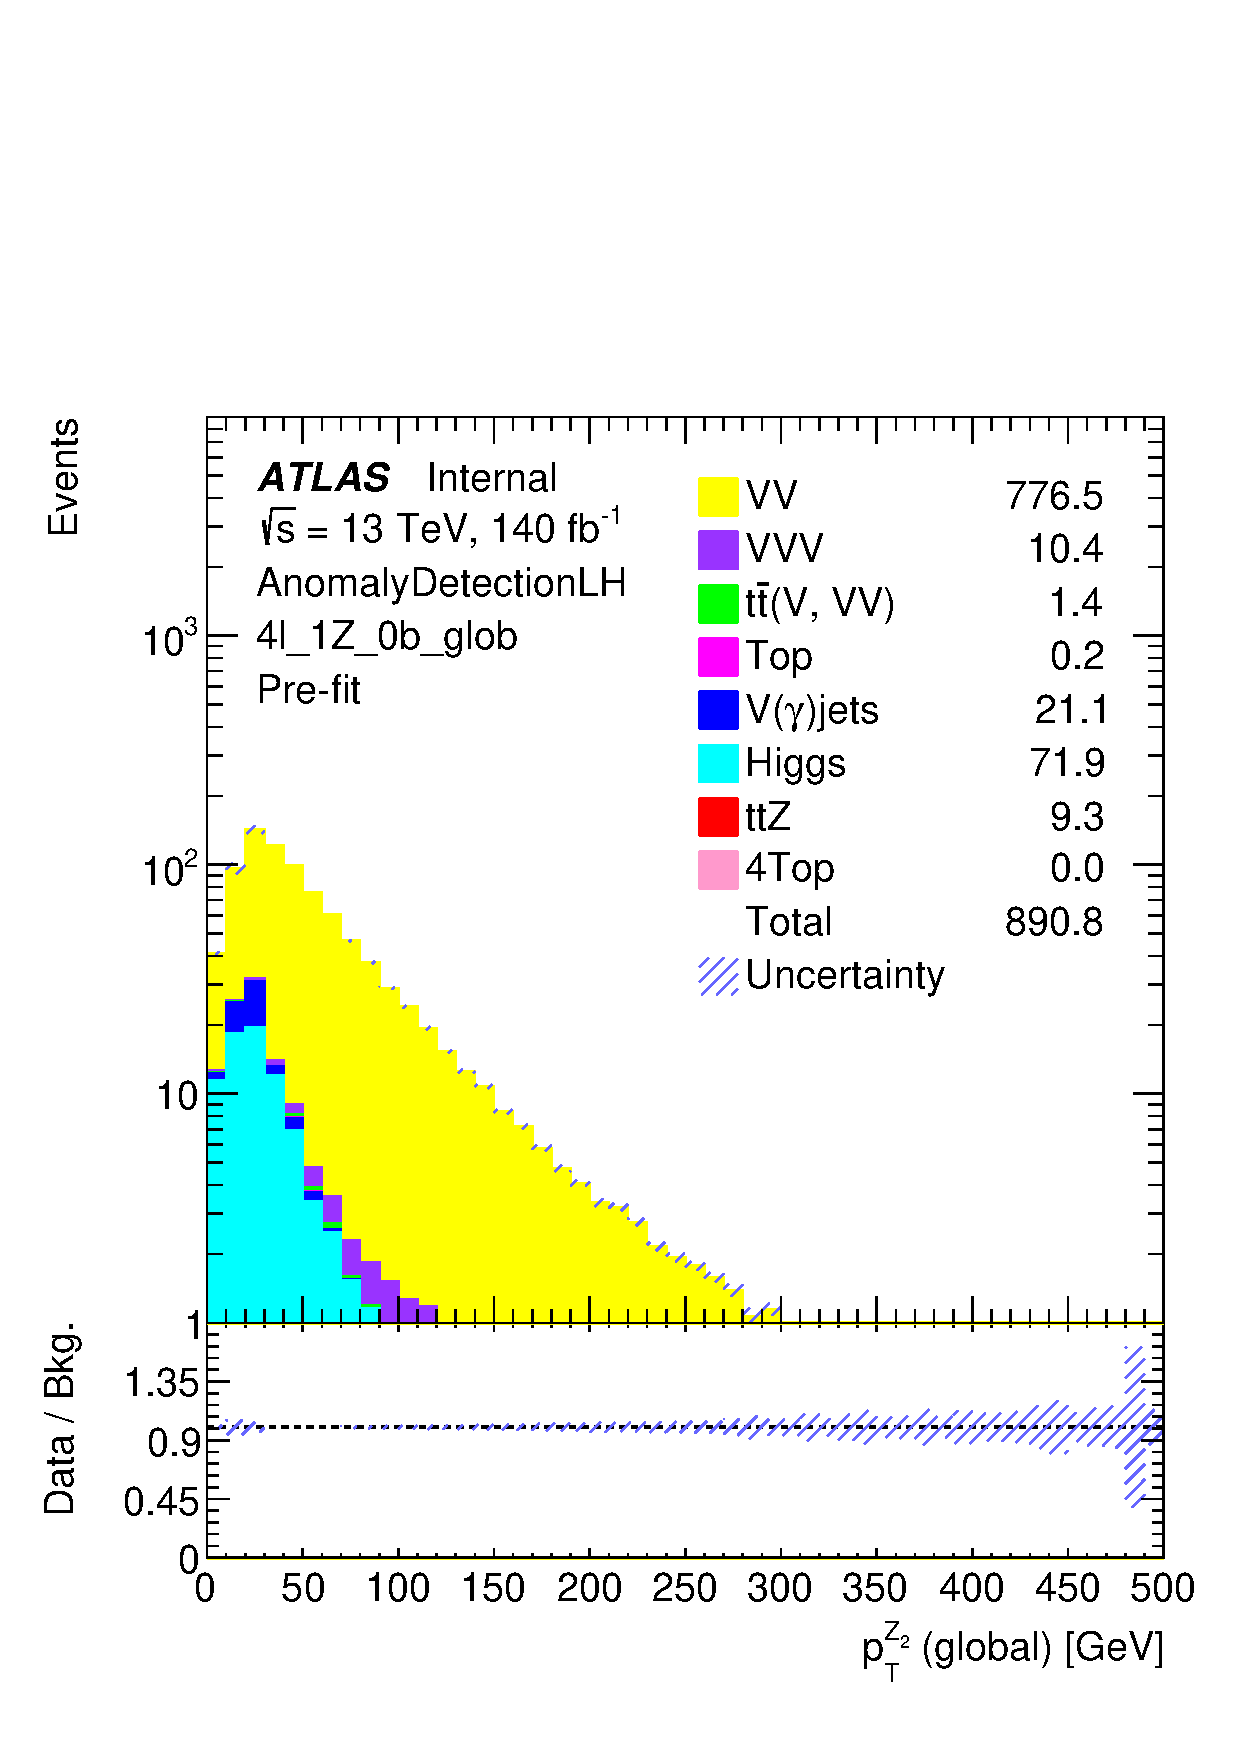
\includegraphics[width=0.24\textwidth]{plots/fourlepLH_run2/Plots/reg_4l_1Z_0b_glob_Z2_pt_glob.pdf}
\end{tabular}
\end{frame}

\begin{frame}{\texttt{Results: 4l\_1Z\_0b}}
\begin{tabular}{cccccc}
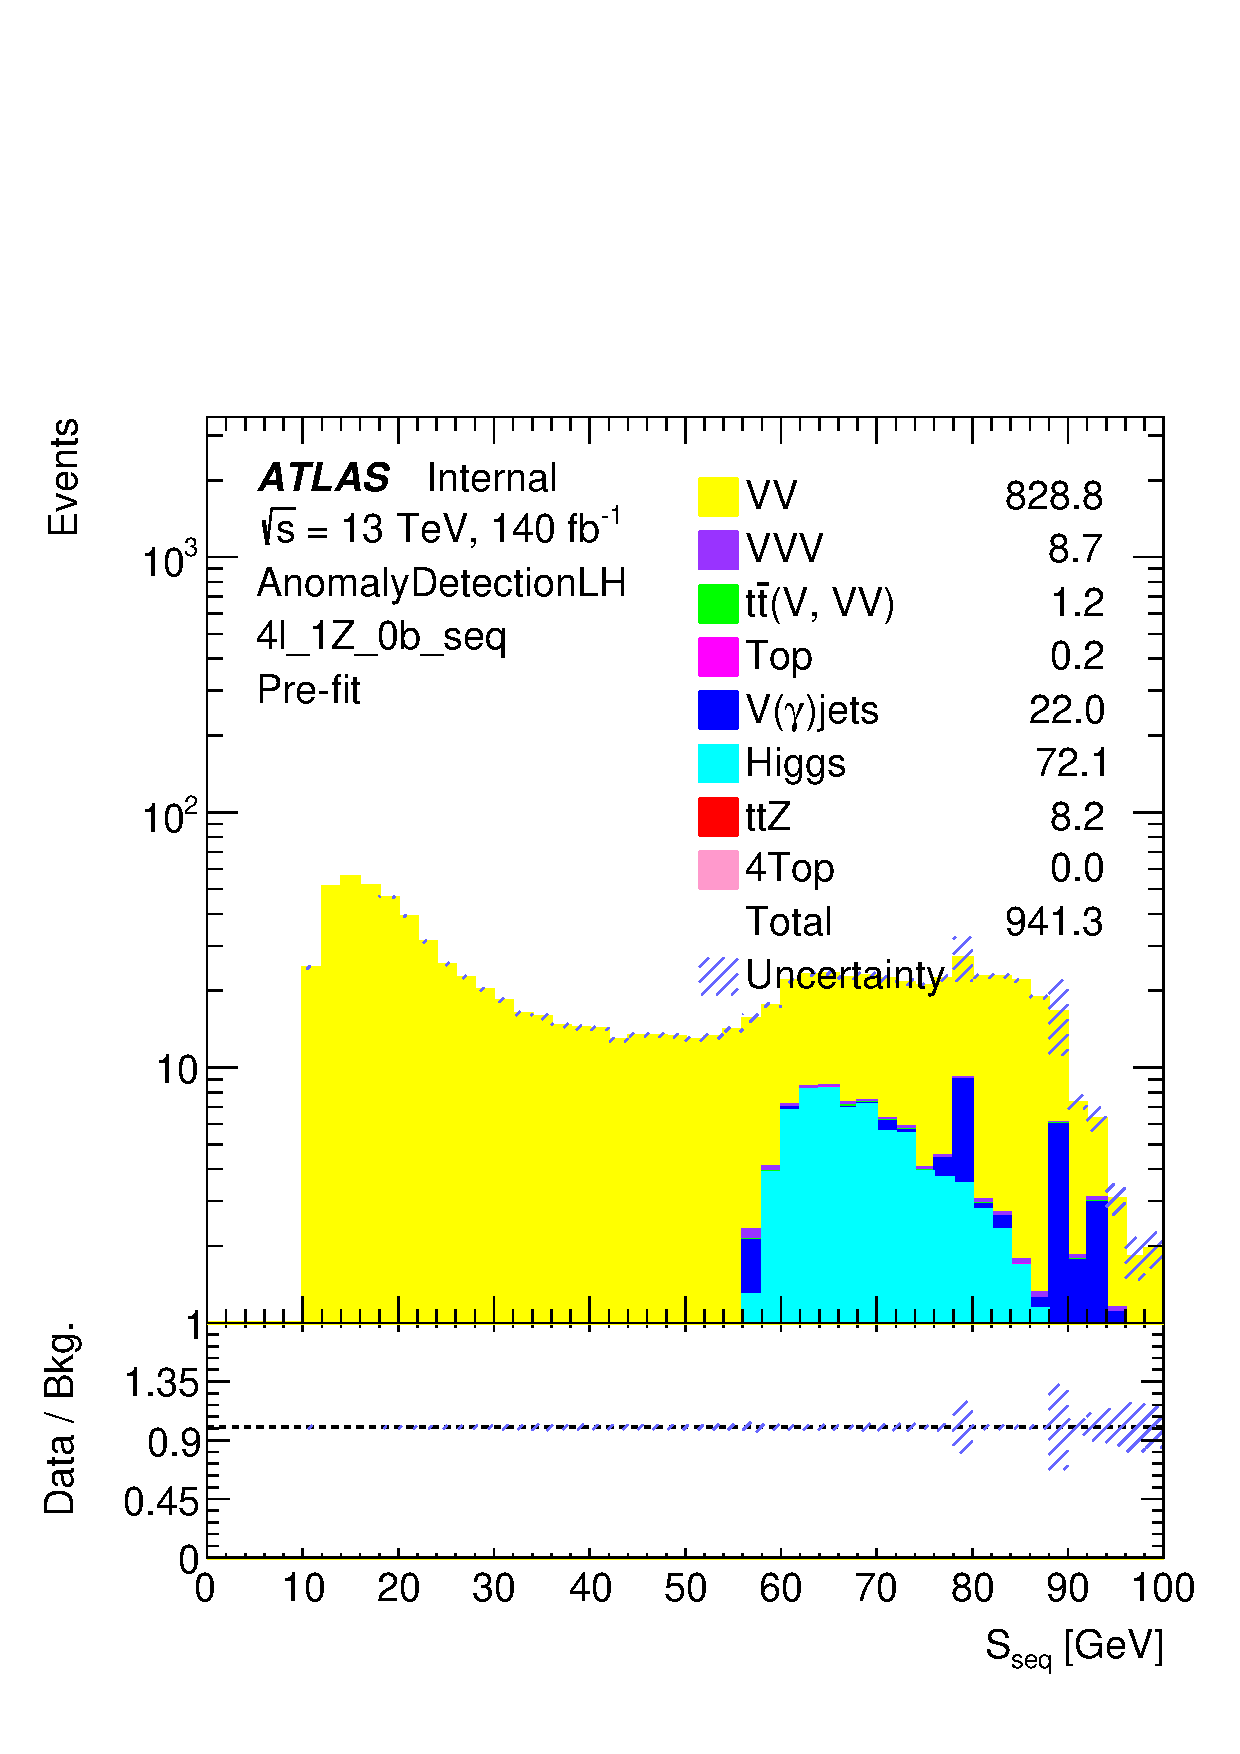
\includegraphics[width=0.24\textwidth]{plots/fourlepLH_run2/Plots/reg_4l_1Z_0b_seq_Zscore_seq.pdf} & 
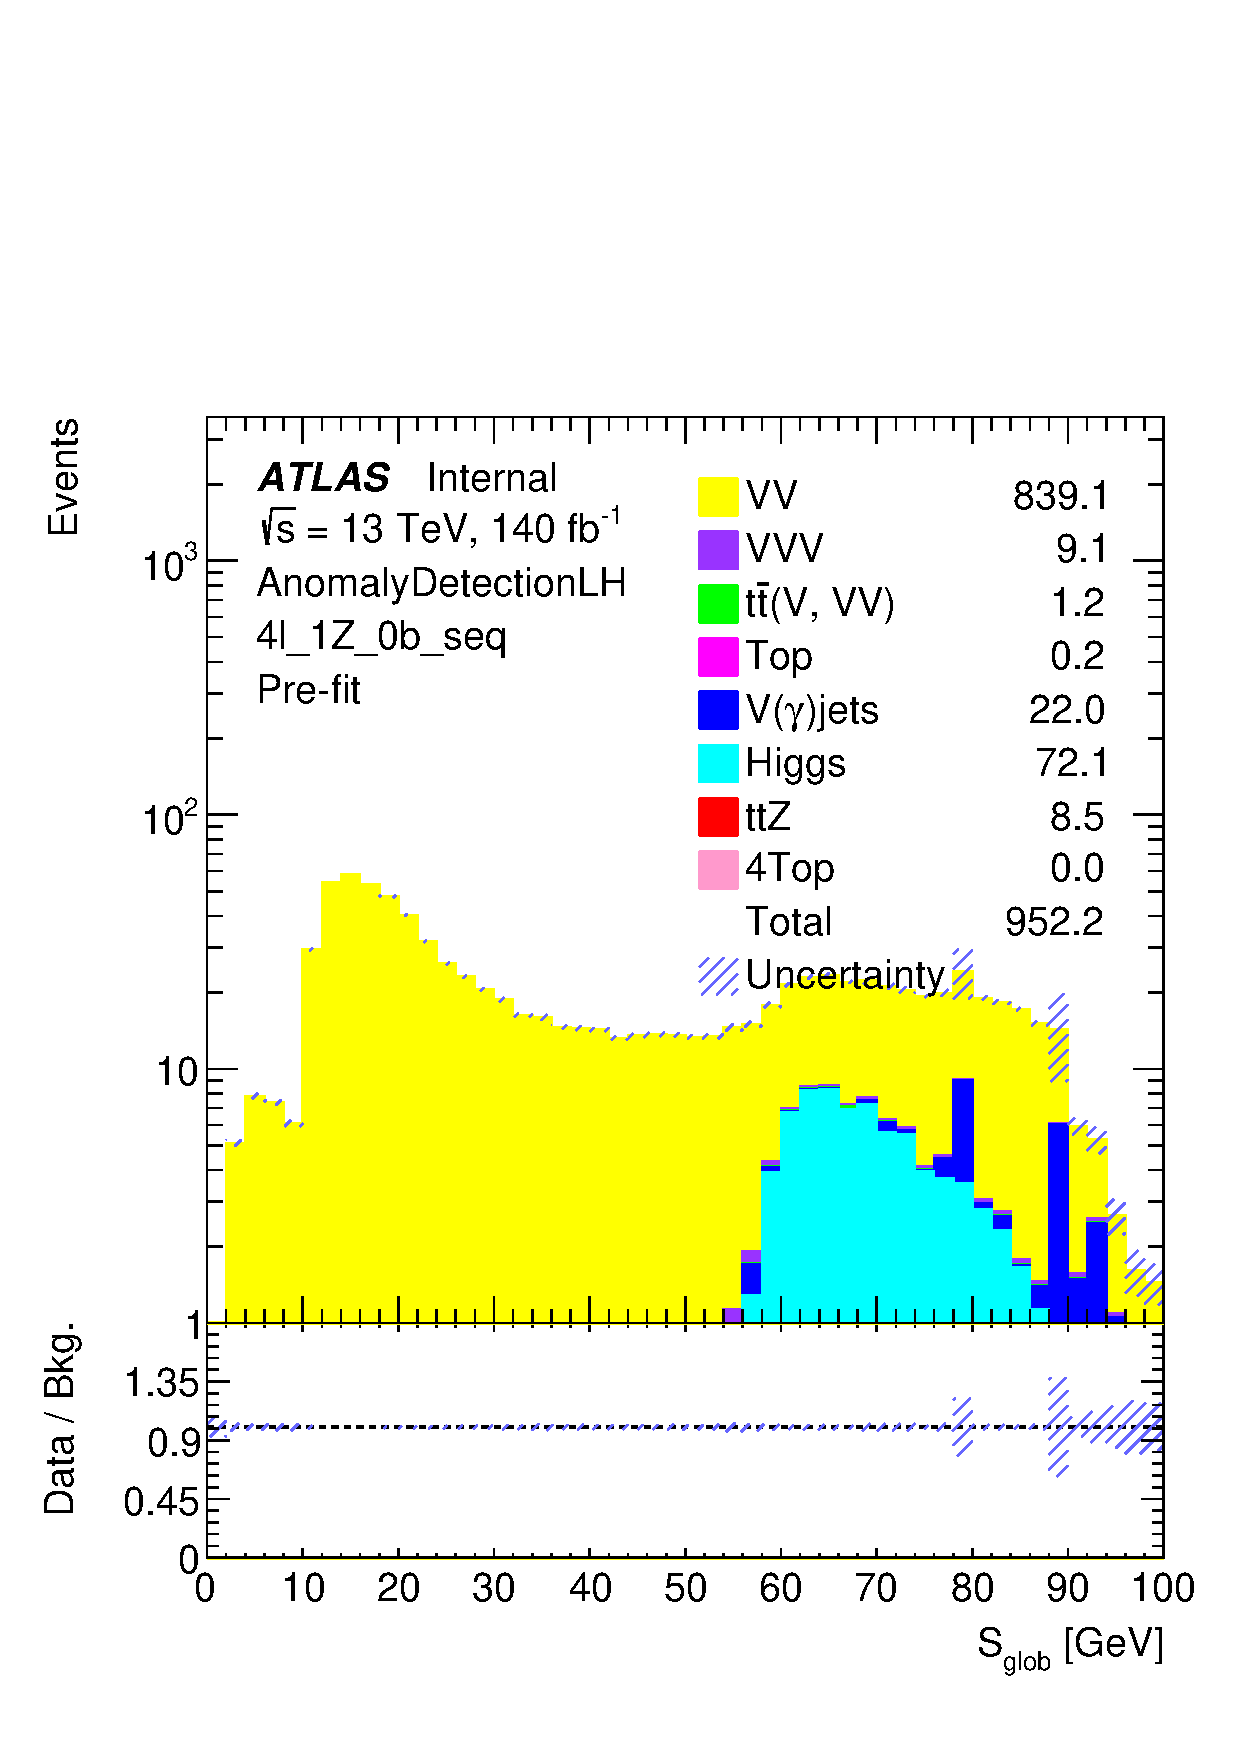
\includegraphics[width=0.24\textwidth]{plots/fourlepLH_run2/Plots/reg_4l_1Z_0b_seq_Zscore_glob.pdf}&
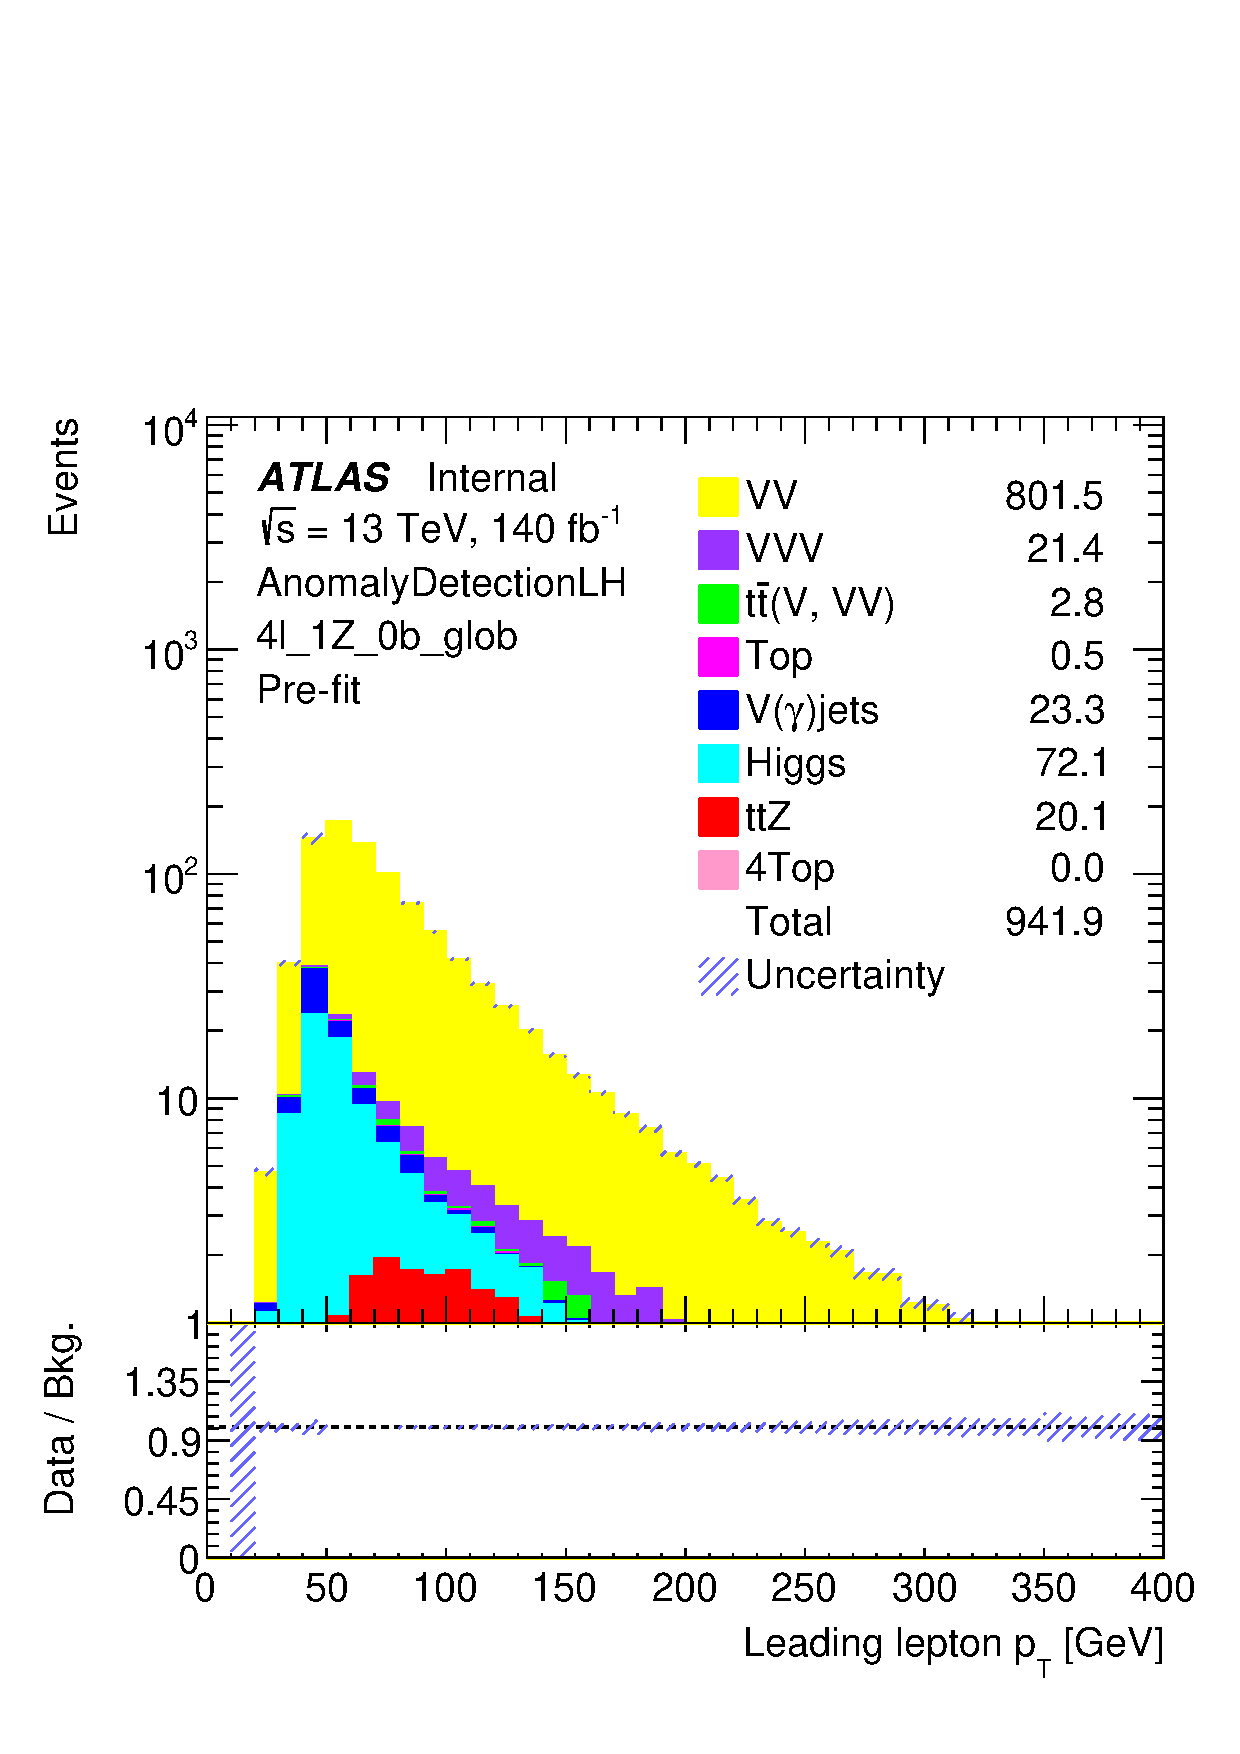
\includegraphics[width=0.24\textwidth]{plots/fourlepLH_run2/Plots/reg_4l_1Z_0b_seq_deltaZscore.pdf}\\

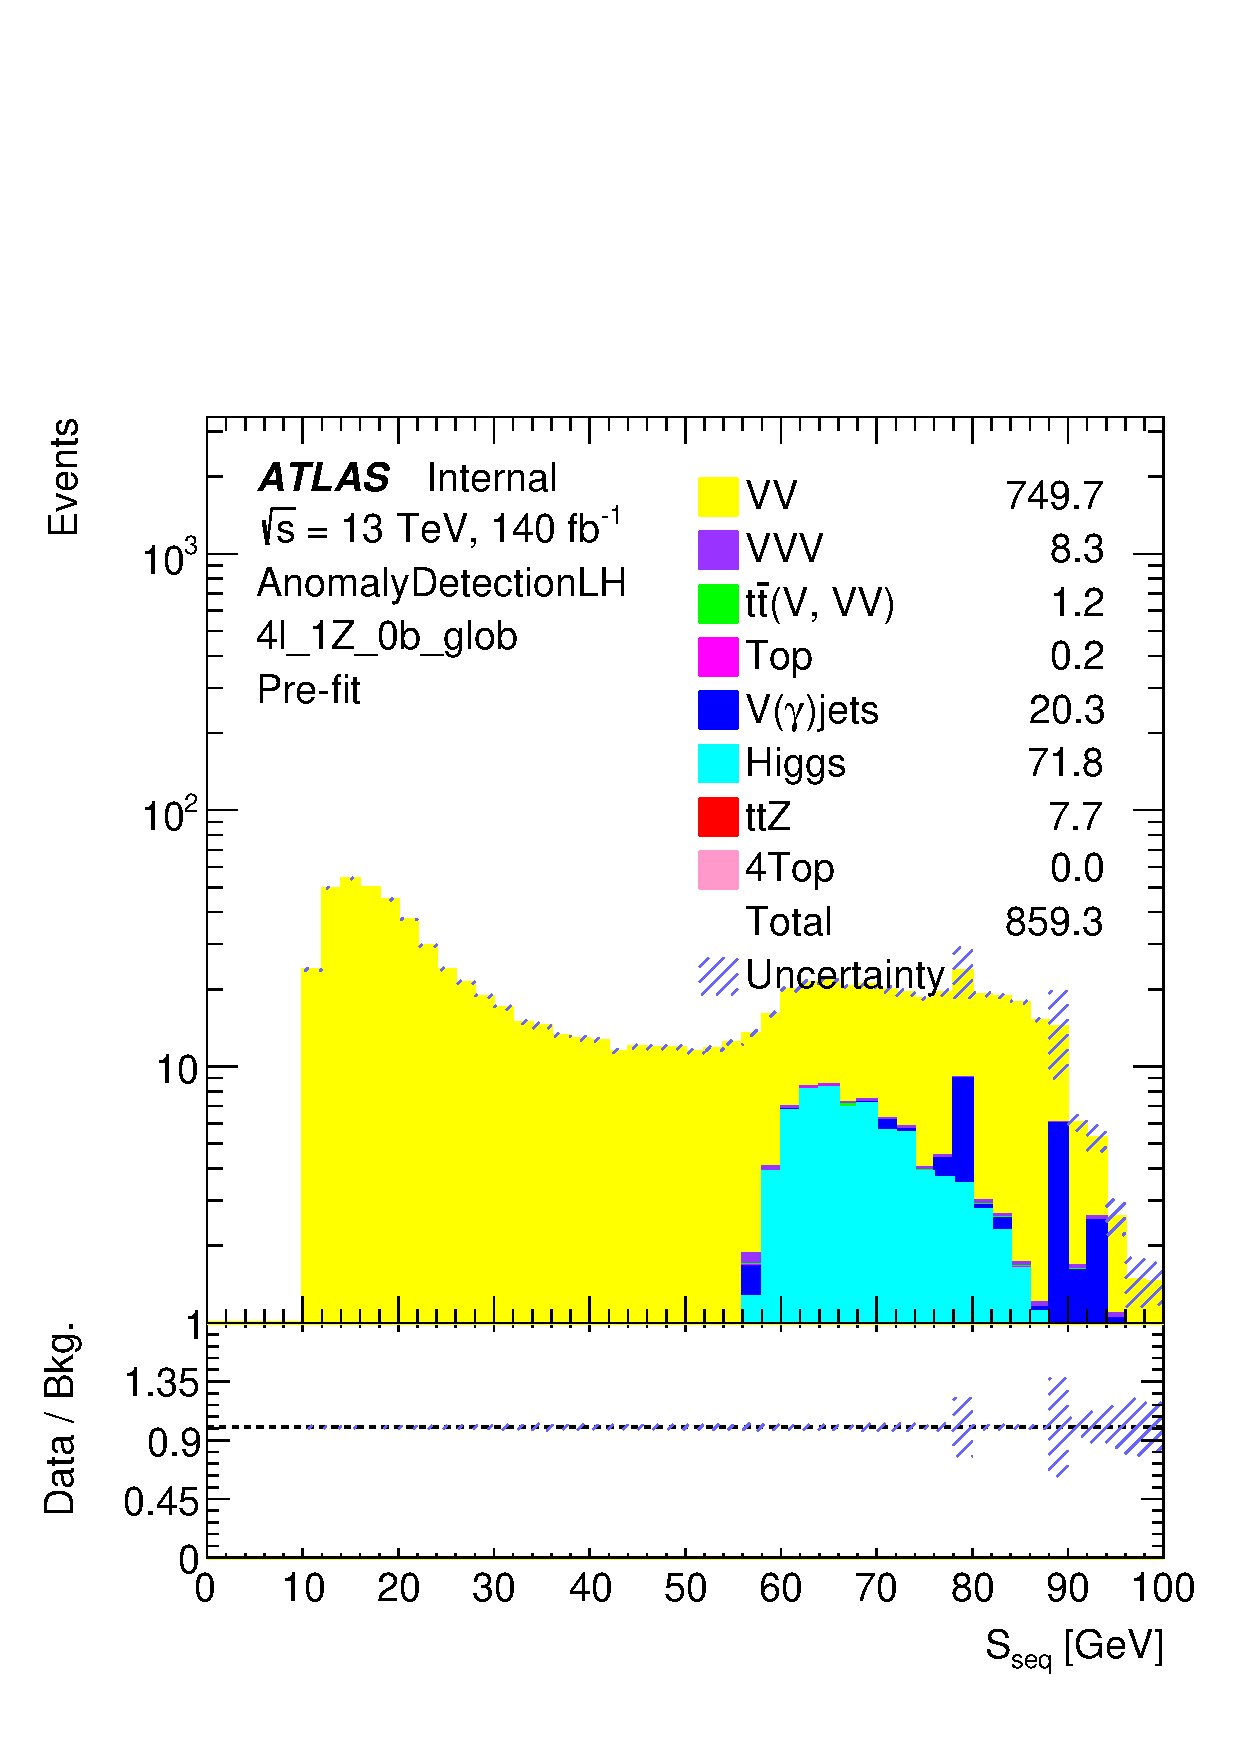
\includegraphics[width=0.24\textwidth]{plots/fourlepLH_run2/Plots/reg_4l_1Z_0b_glob_Zscore_seq.pdf} & 
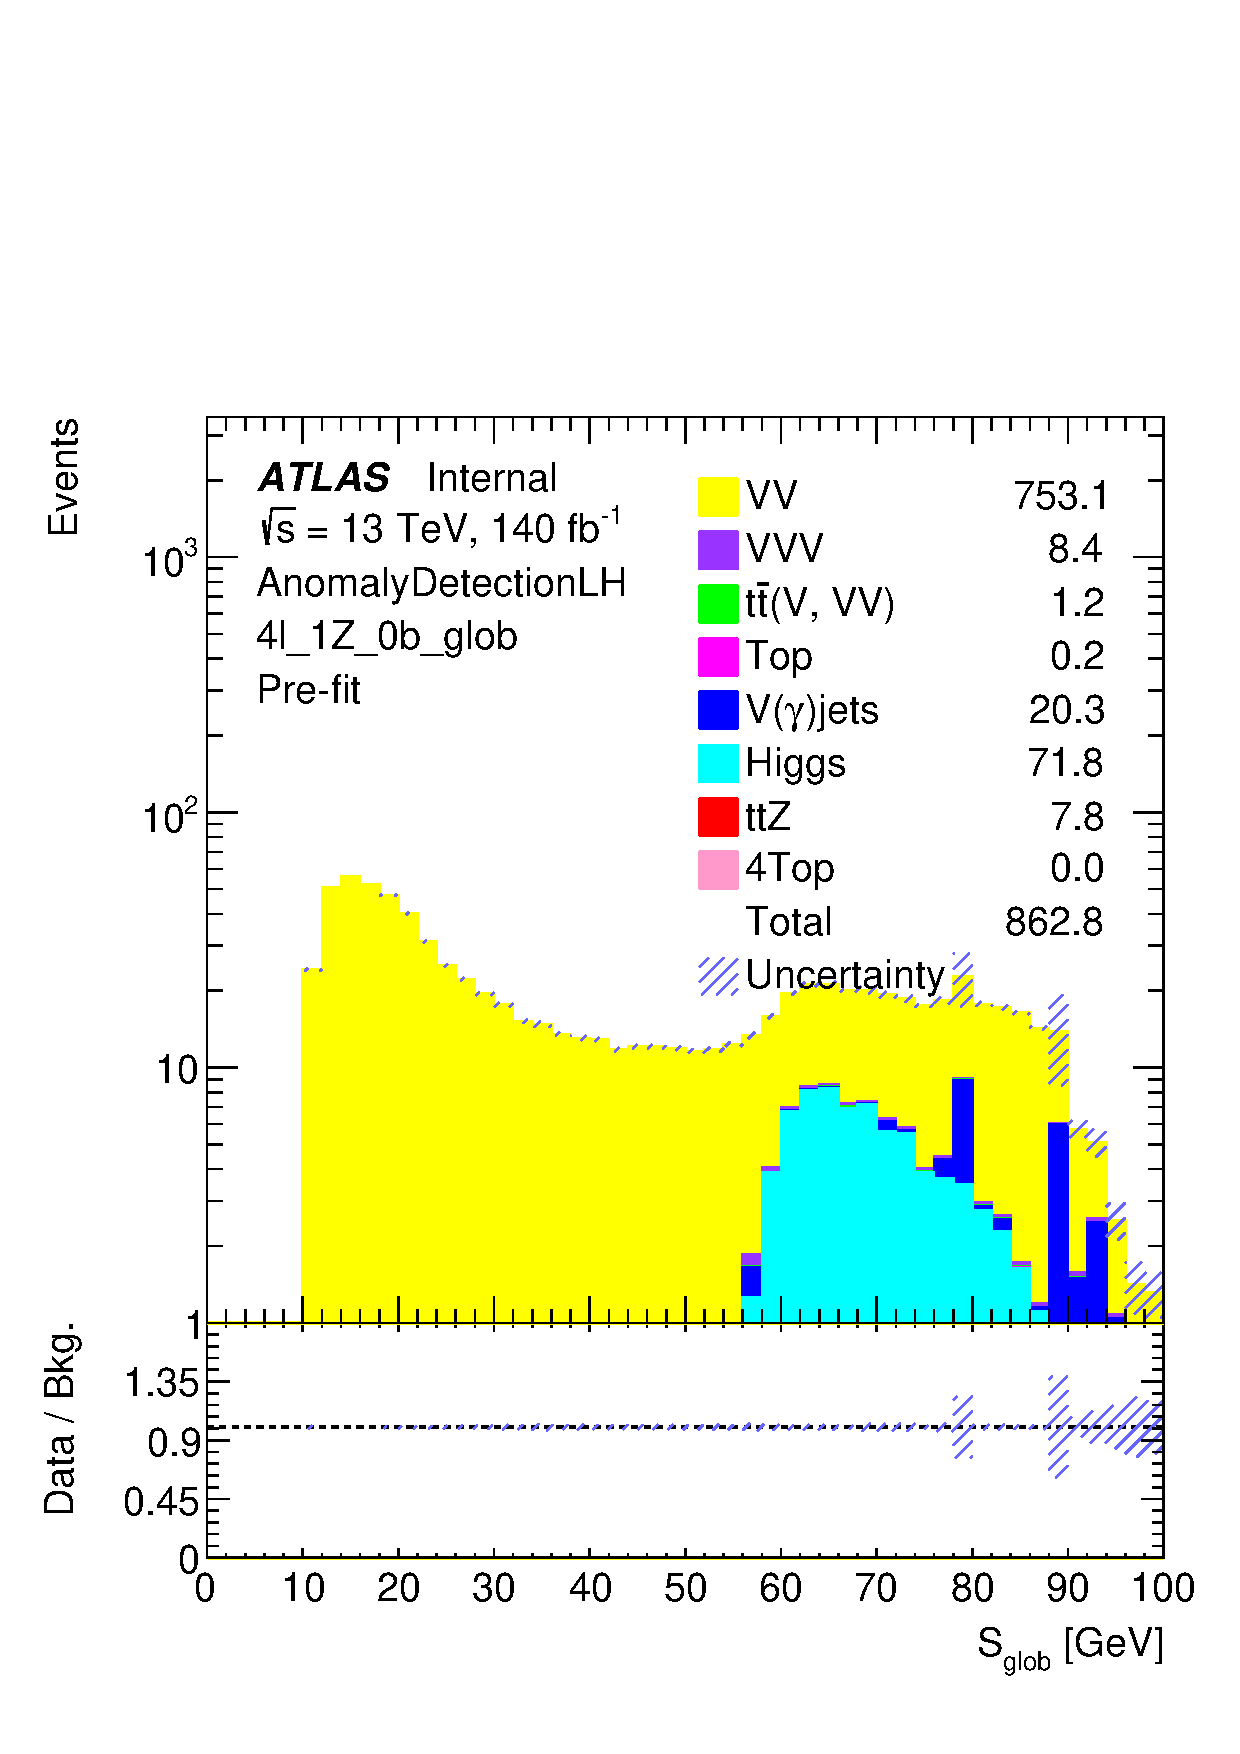
\includegraphics[width=0.24\textwidth]{plots/fourlepLH_run2/Plots/reg_4l_1Z_0b_glob_Zscore_glob.pdf}&
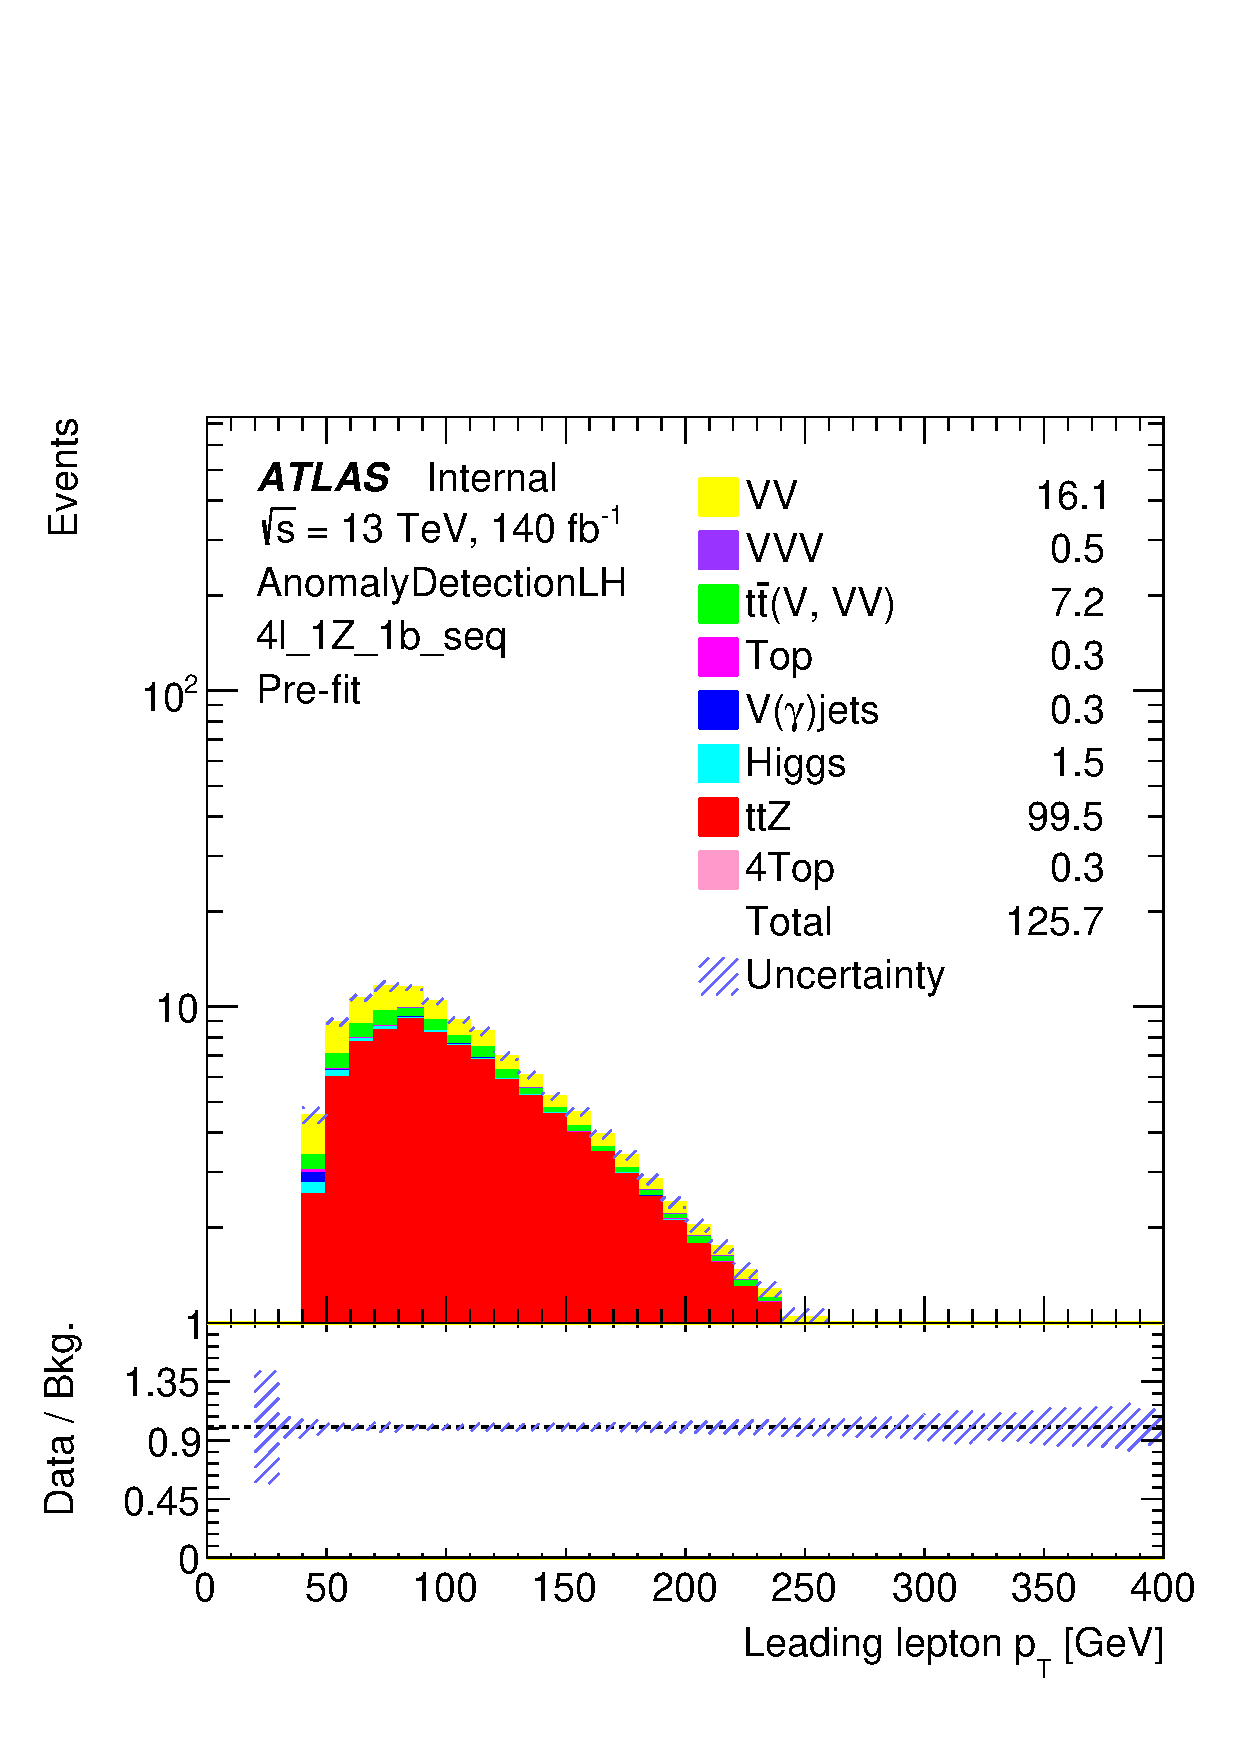
\includegraphics[width=0.24\textwidth]{plots/fourlepLH_run2/Plots/reg_4l_1Z_0b_glob_deltaZscore.pdf}
\end{tabular}
\end{frame}


\begin{frame}{\texttt{Results: 4l\_1Z\_0b}}
\begin{tabular}{cccccc}

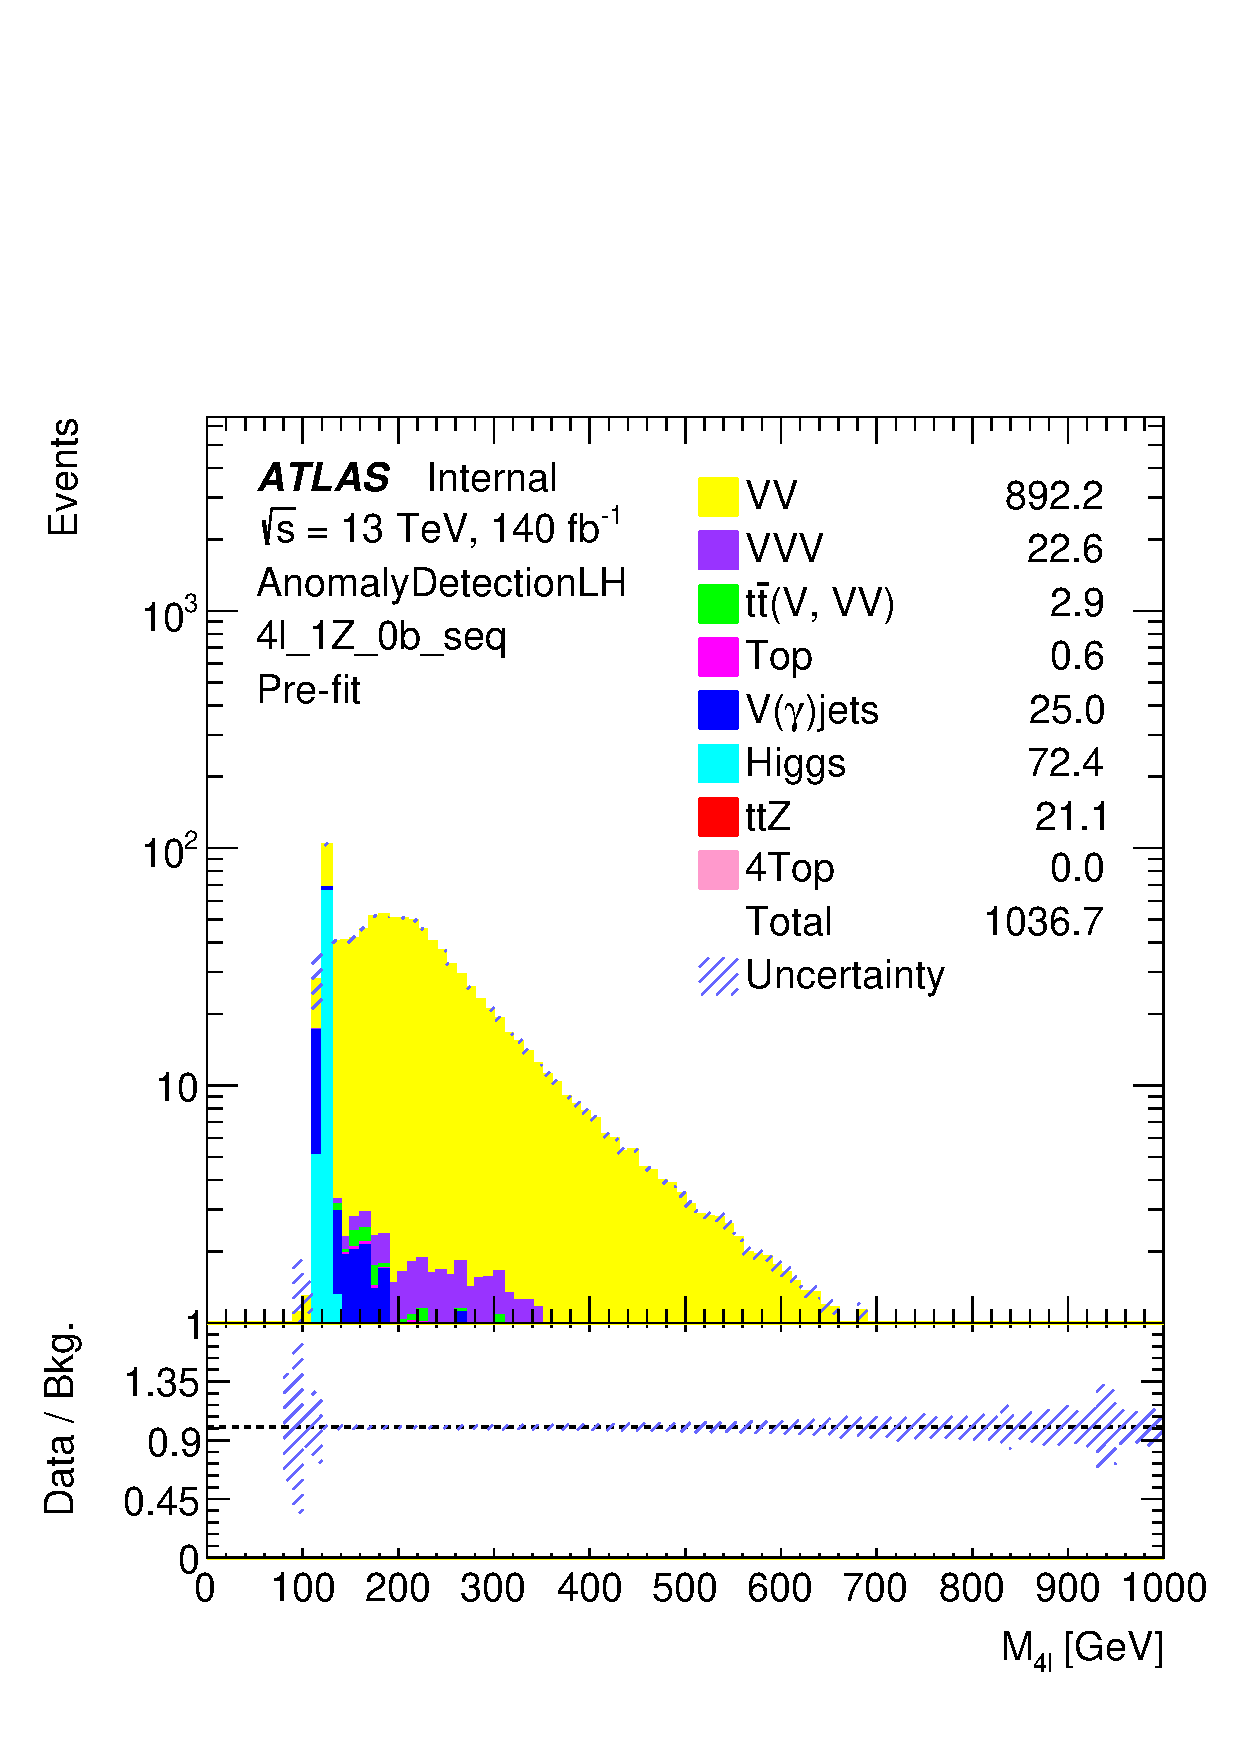
\includegraphics[width=0.24\textwidth]{plots/fourlepLH_run2/Plots/reg_4l_1Z_0b_seq_m4l.pdf} &
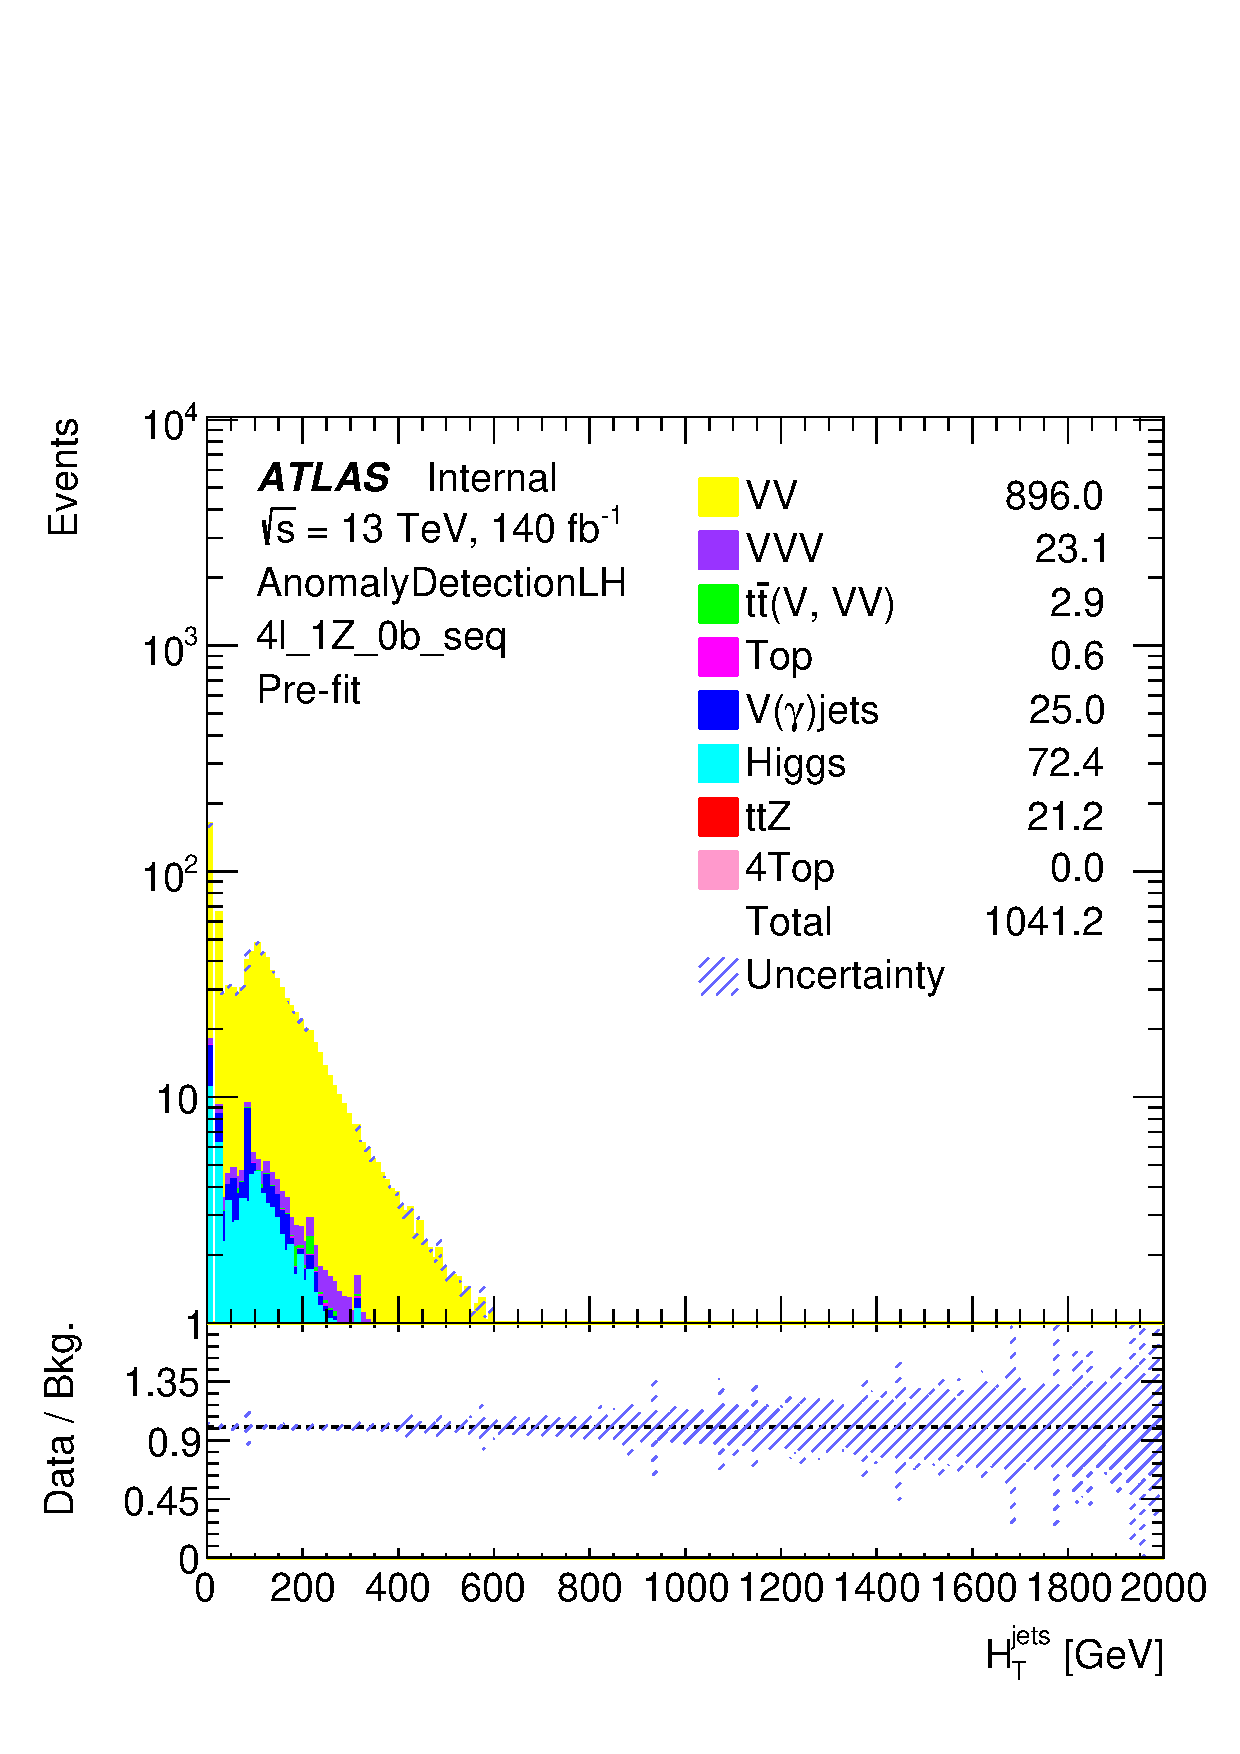
\includegraphics[width=0.24\textwidth]{plots/fourlepLH_run2/Plots/reg_4l_1Z_0b_seq_HT_jets.pdf} &
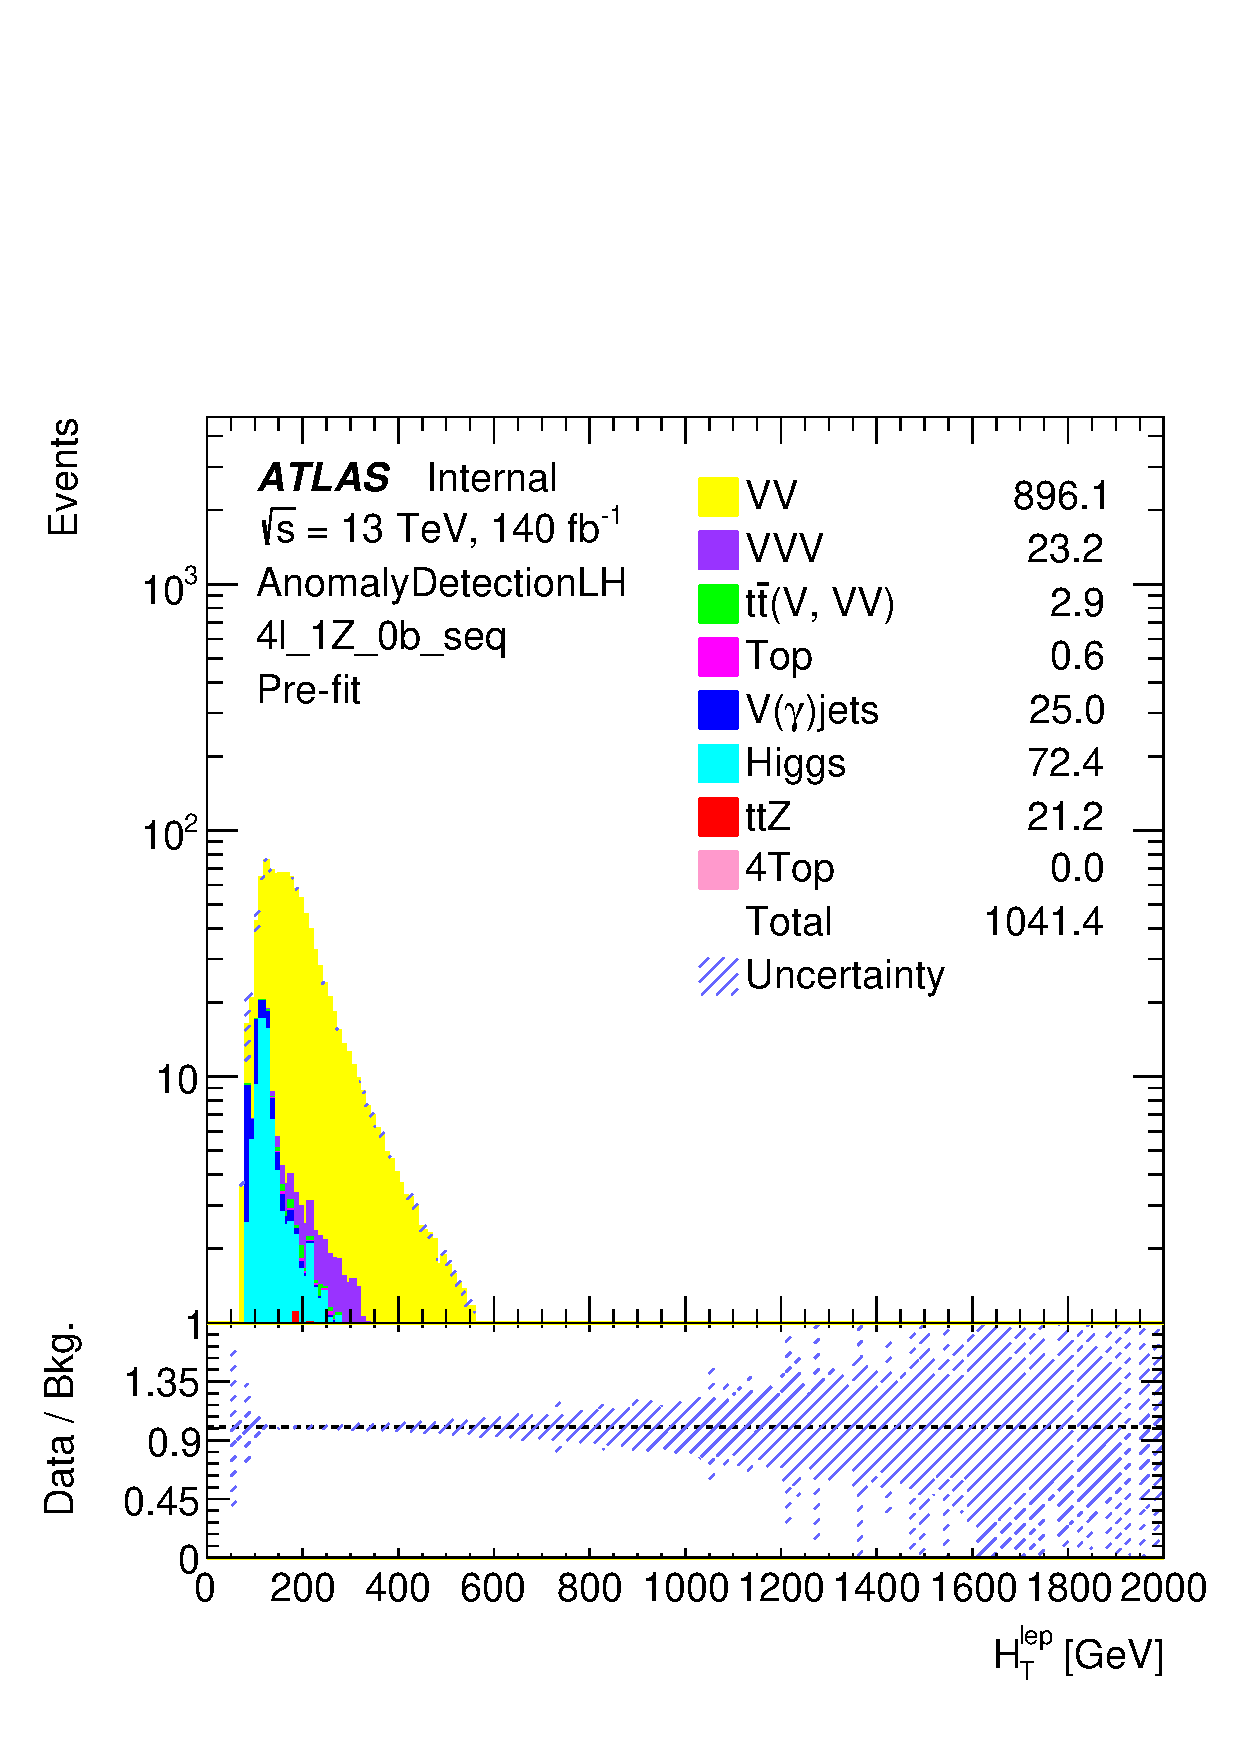
\includegraphics[width=0.24\textwidth]{plots/fourlepLH_run2/Plots/reg_4l_1Z_0b_seq_HT_lep.pdf} &
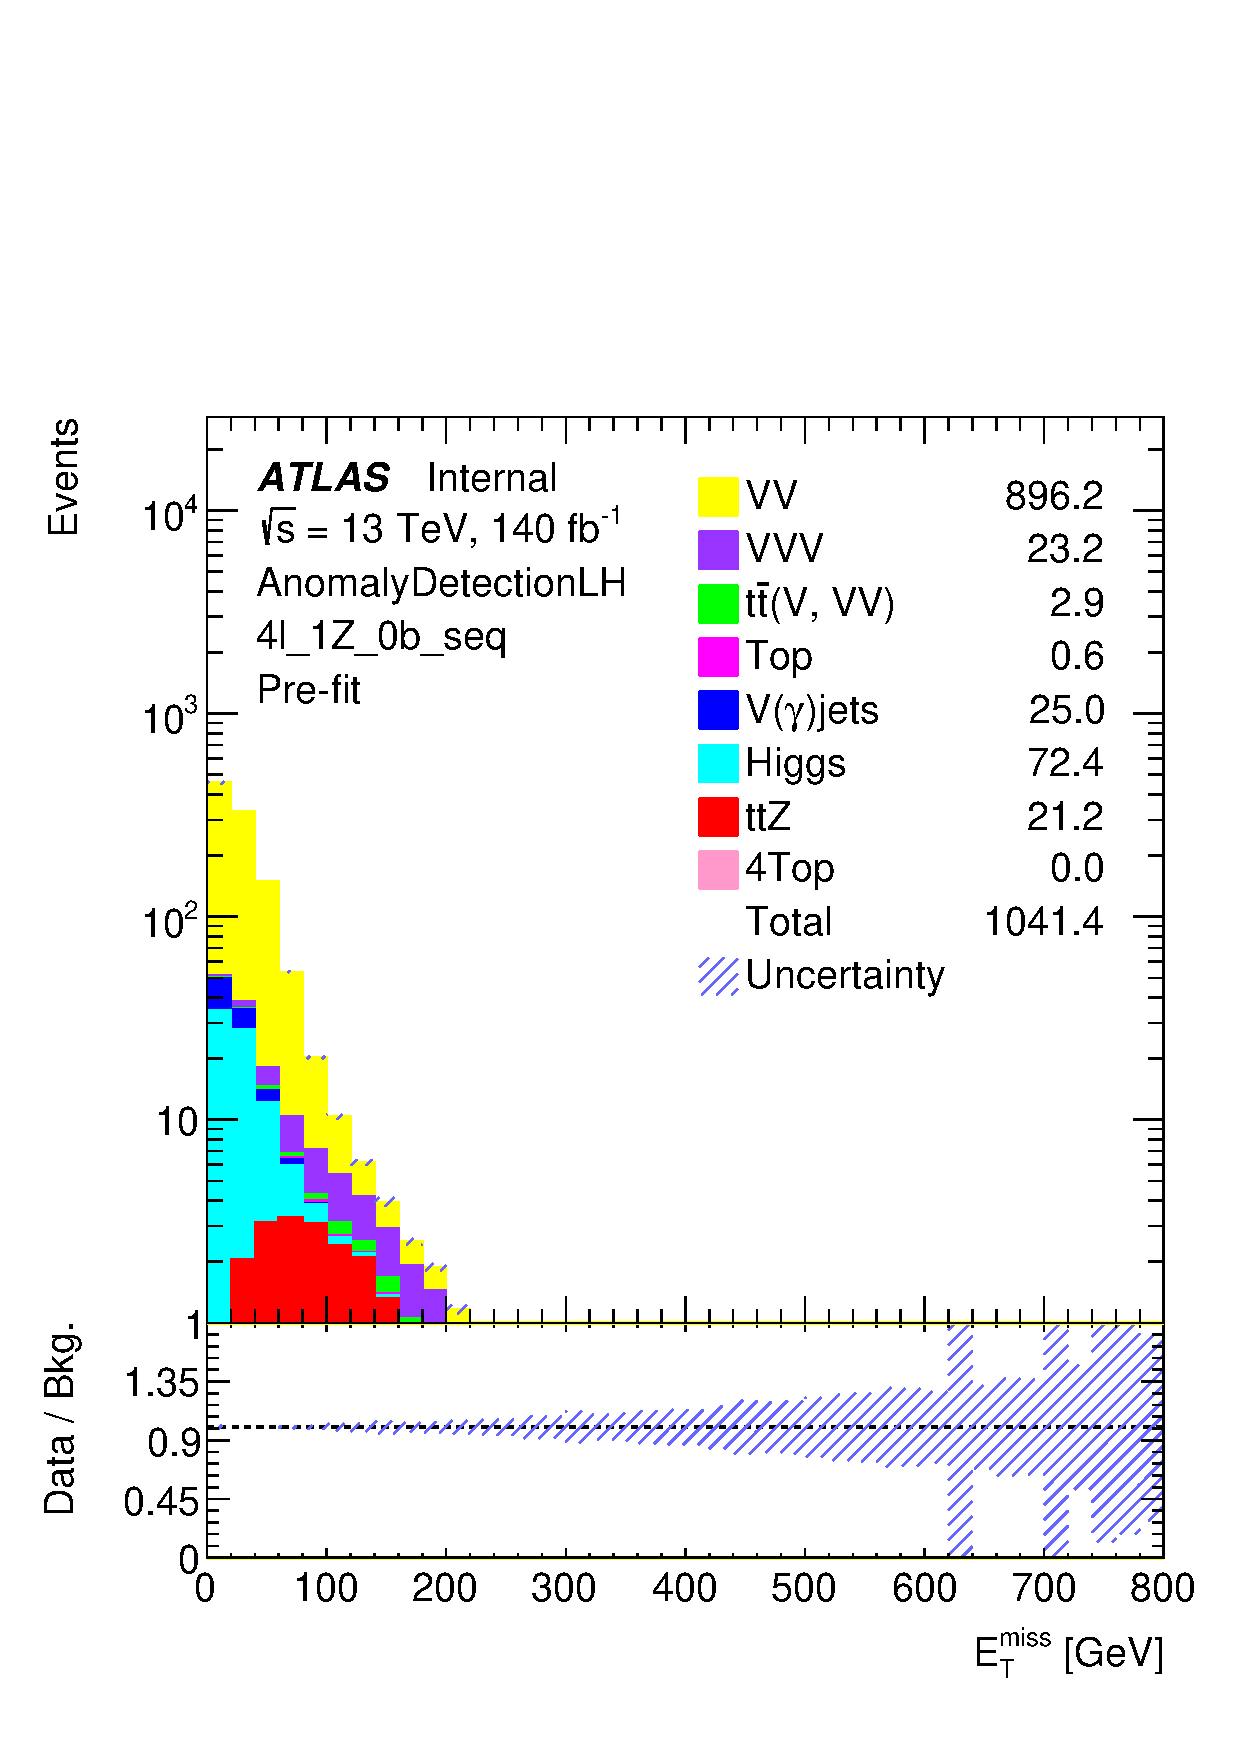
\includegraphics[width=0.24\textwidth]{plots/fourlepLH_run2/Plots/reg_4l_1Z_0b_seq_met.pdf} \\

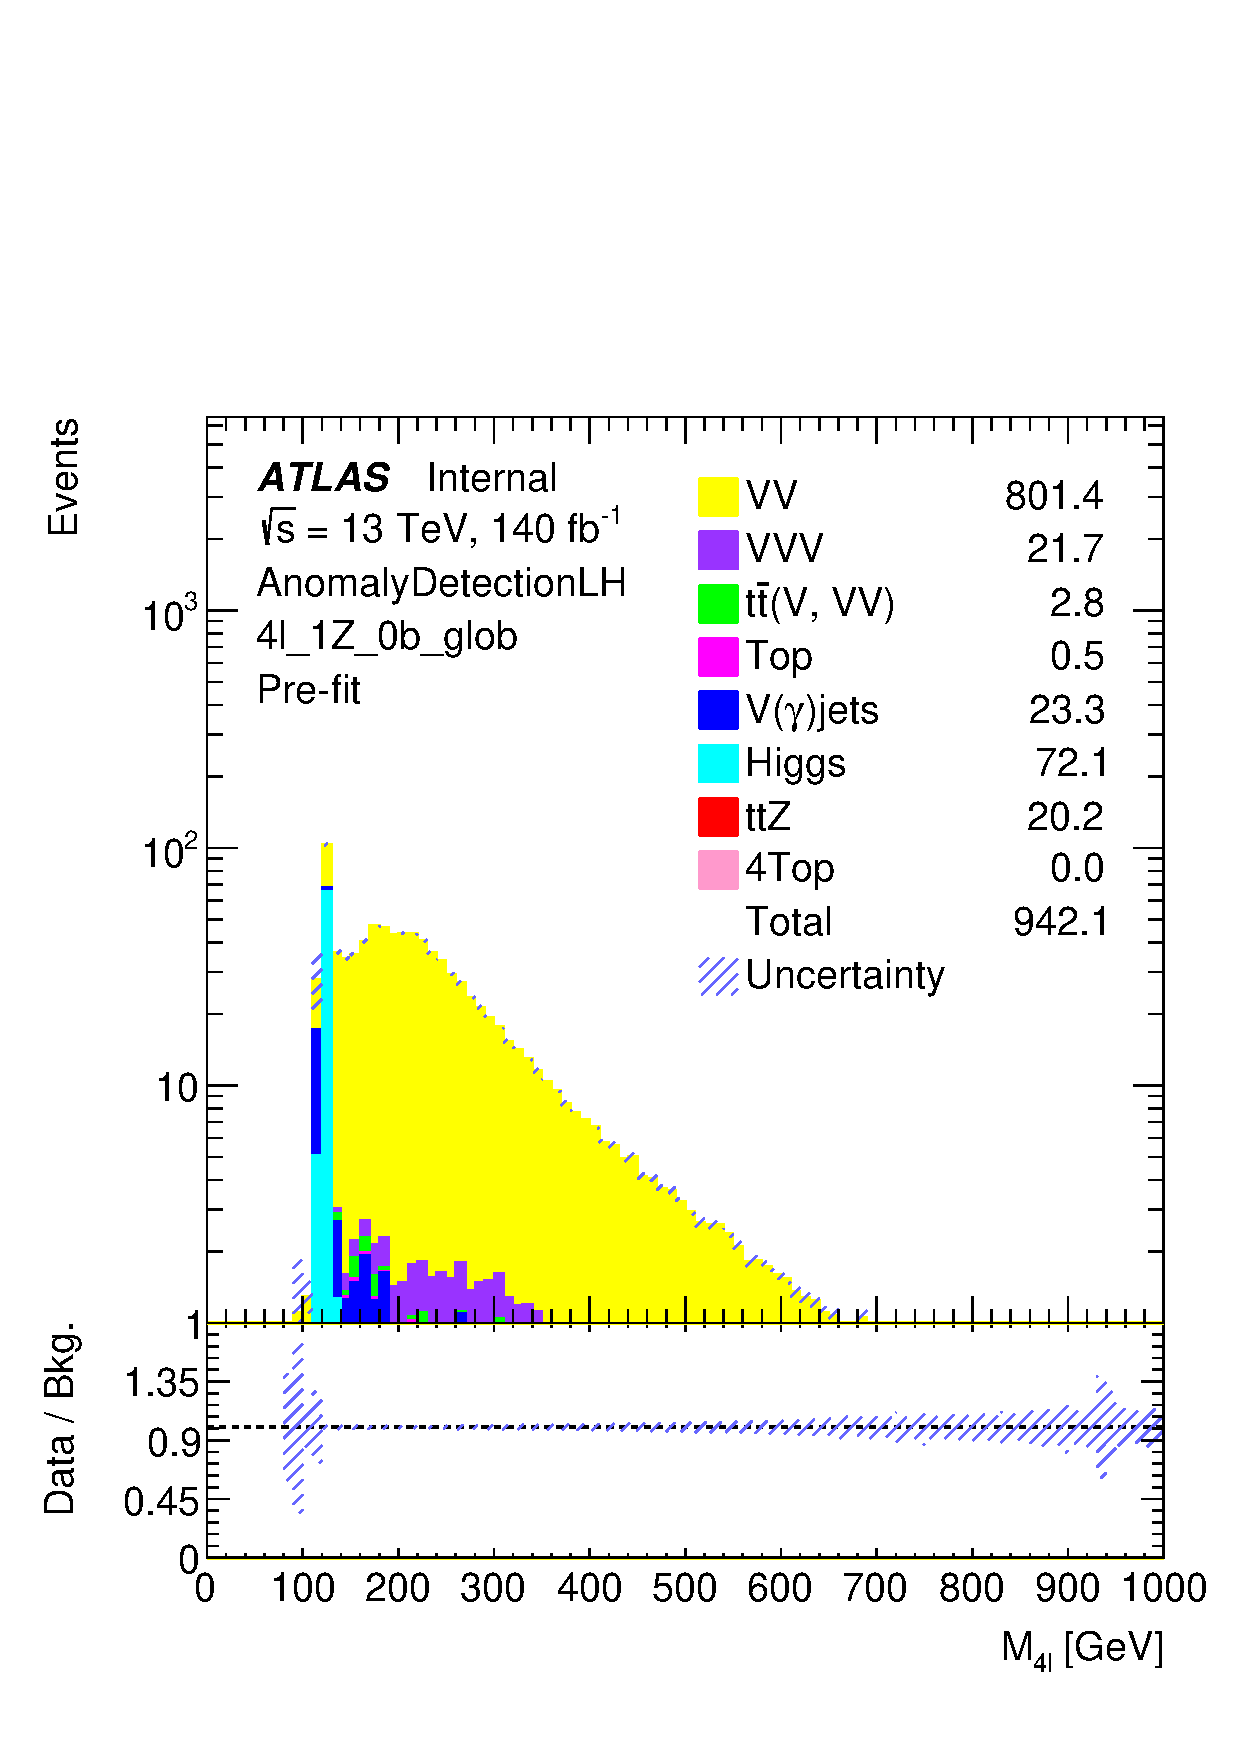
\includegraphics[width=0.24\textwidth]{plots/fourlepLH_run2/Plots/reg_4l_1Z_0b_glob_m4l.pdf} &
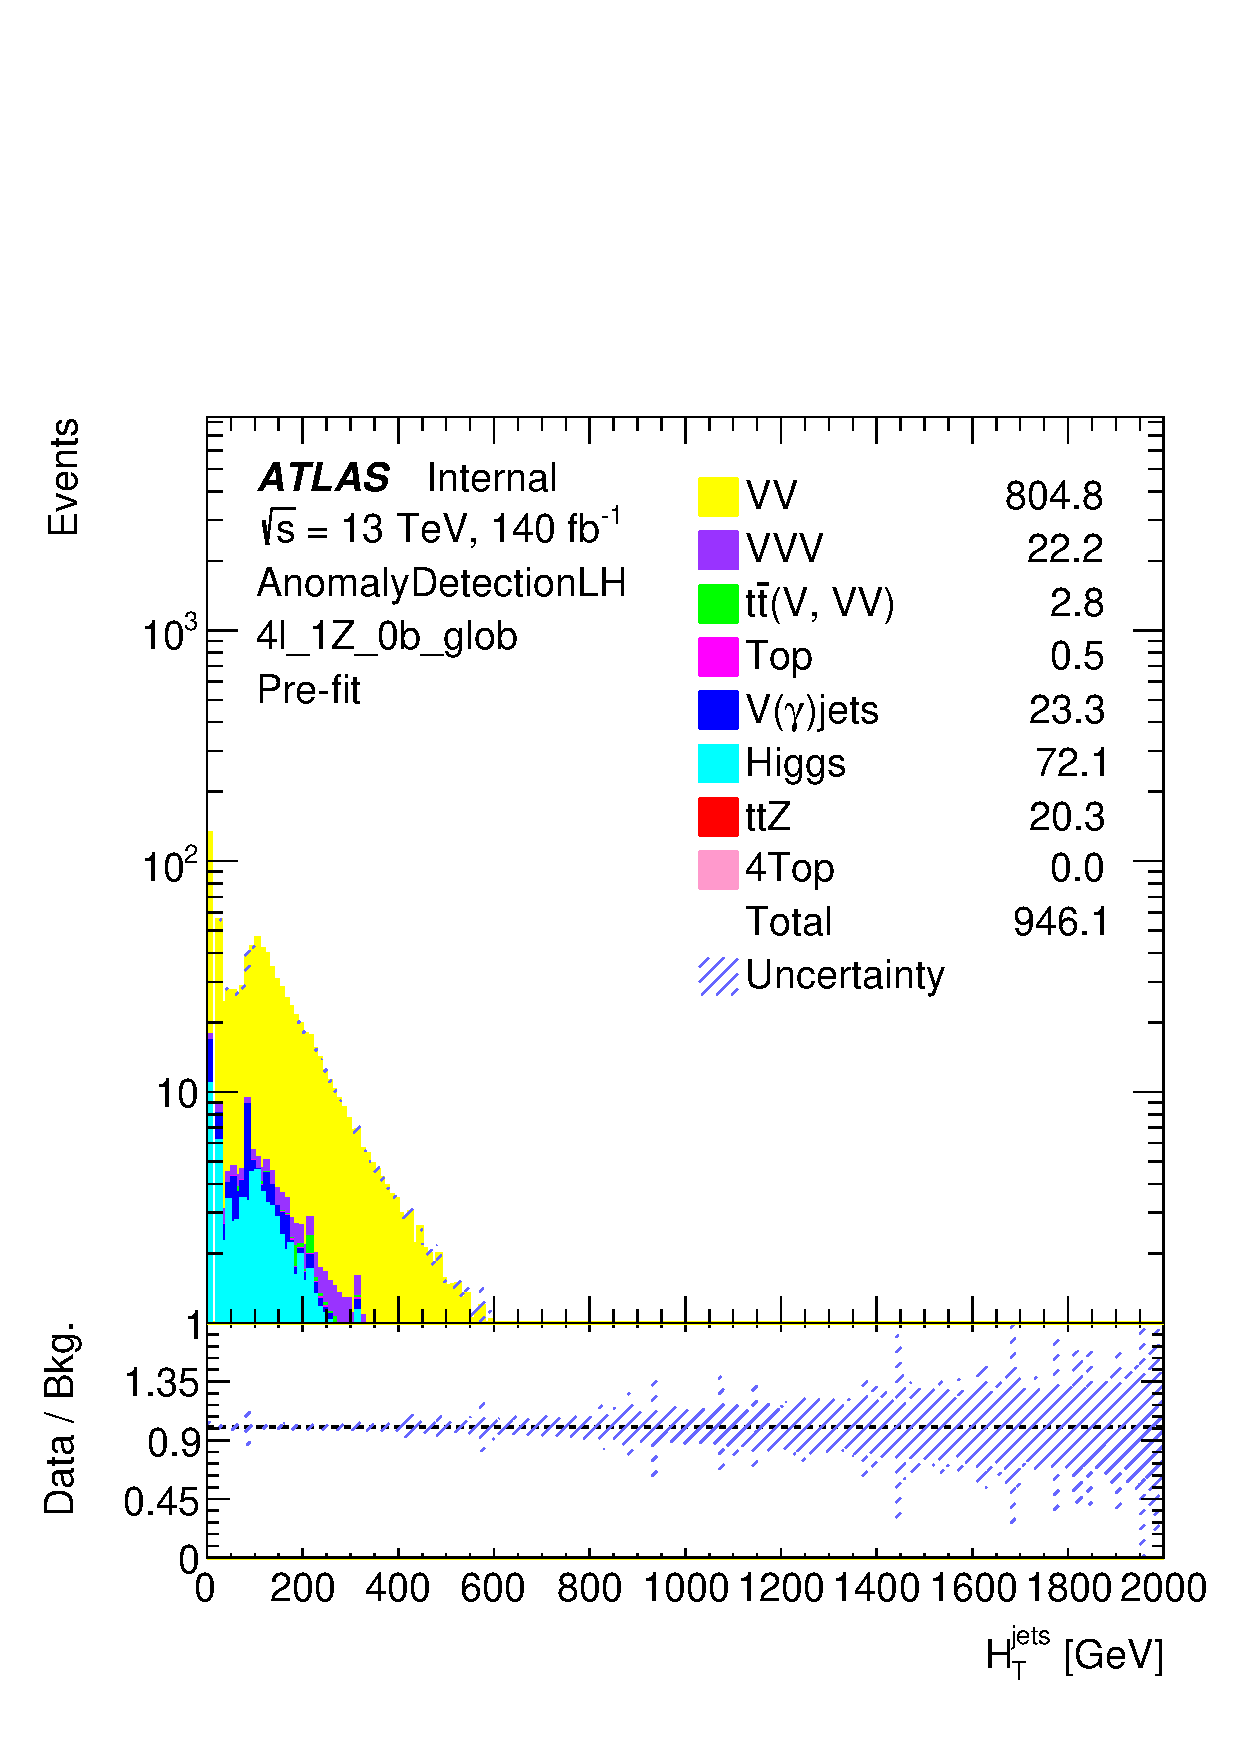
\includegraphics[width=0.24\textwidth]{plots/fourlepLH_run2/Plots/reg_4l_1Z_0b_glob_HT_jets.pdf} &
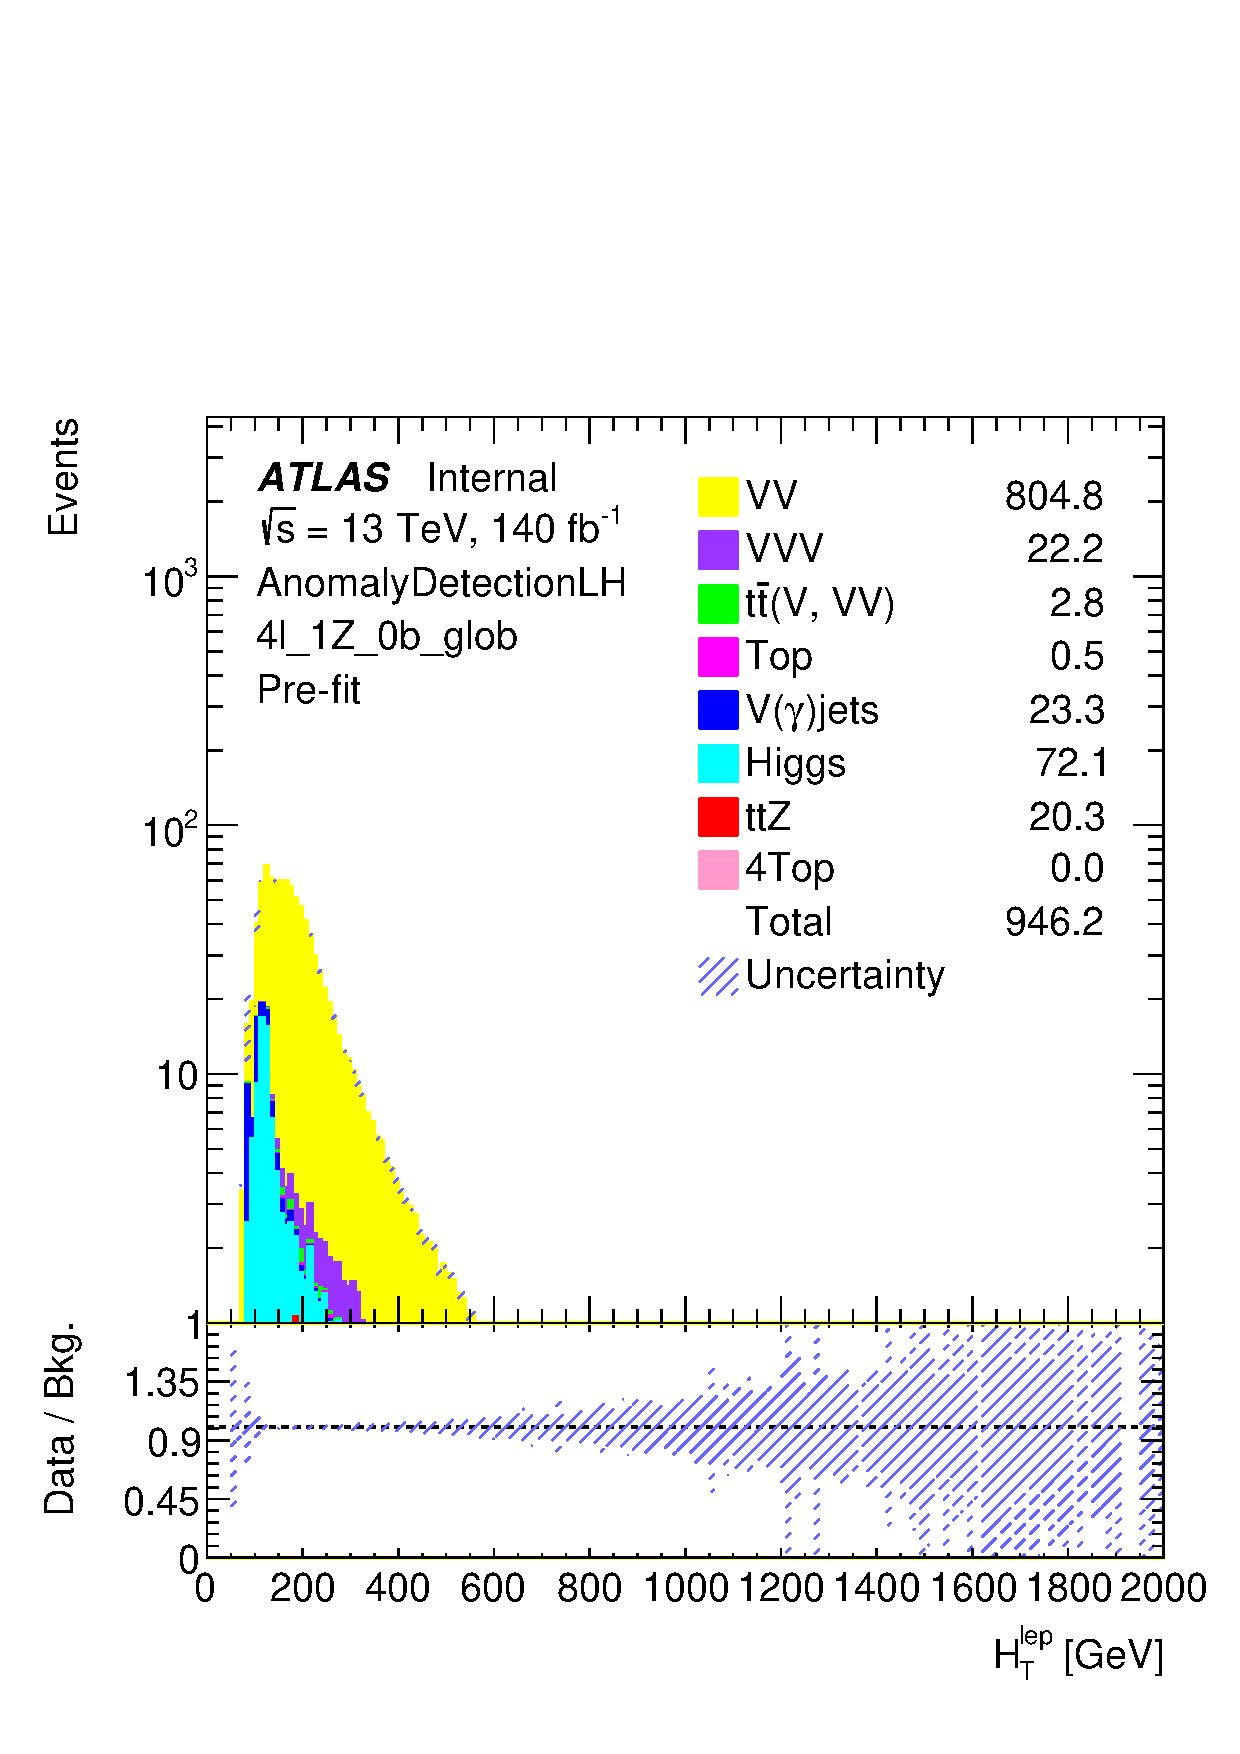
\includegraphics[width=0.24\textwidth]{plots/fourlepLH_run2/Plots/reg_4l_1Z_0b_glob_HT_lep.pdf} &
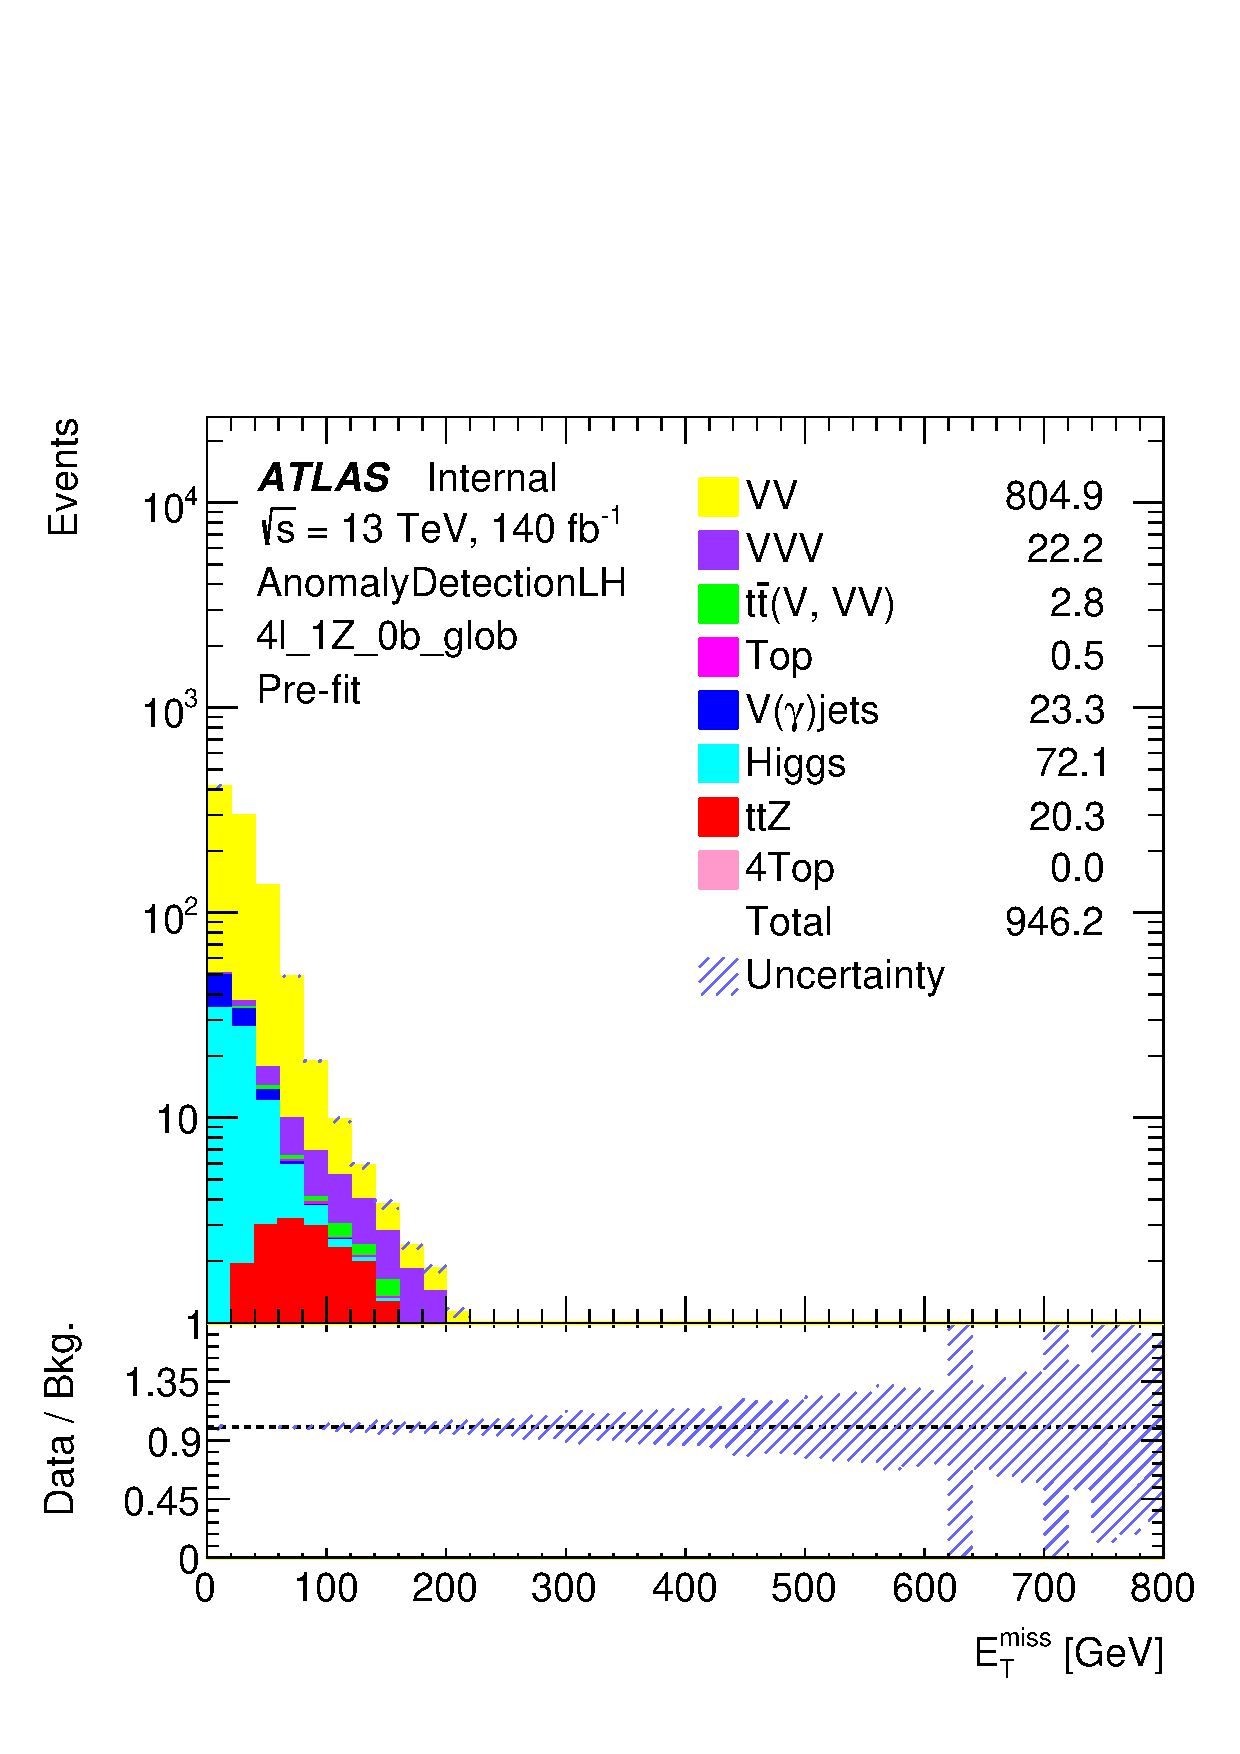
\includegraphics[width=0.24\textwidth]{plots/fourlepLH_run2/Plots/reg_4l_1Z_0b_glob_met.pdf} \\

\end{tabular}
\end{frame}

\begin{frame}{\texttt{Results: 4l\_1Z\_0b}}
\begin{tabular}{cccccc}
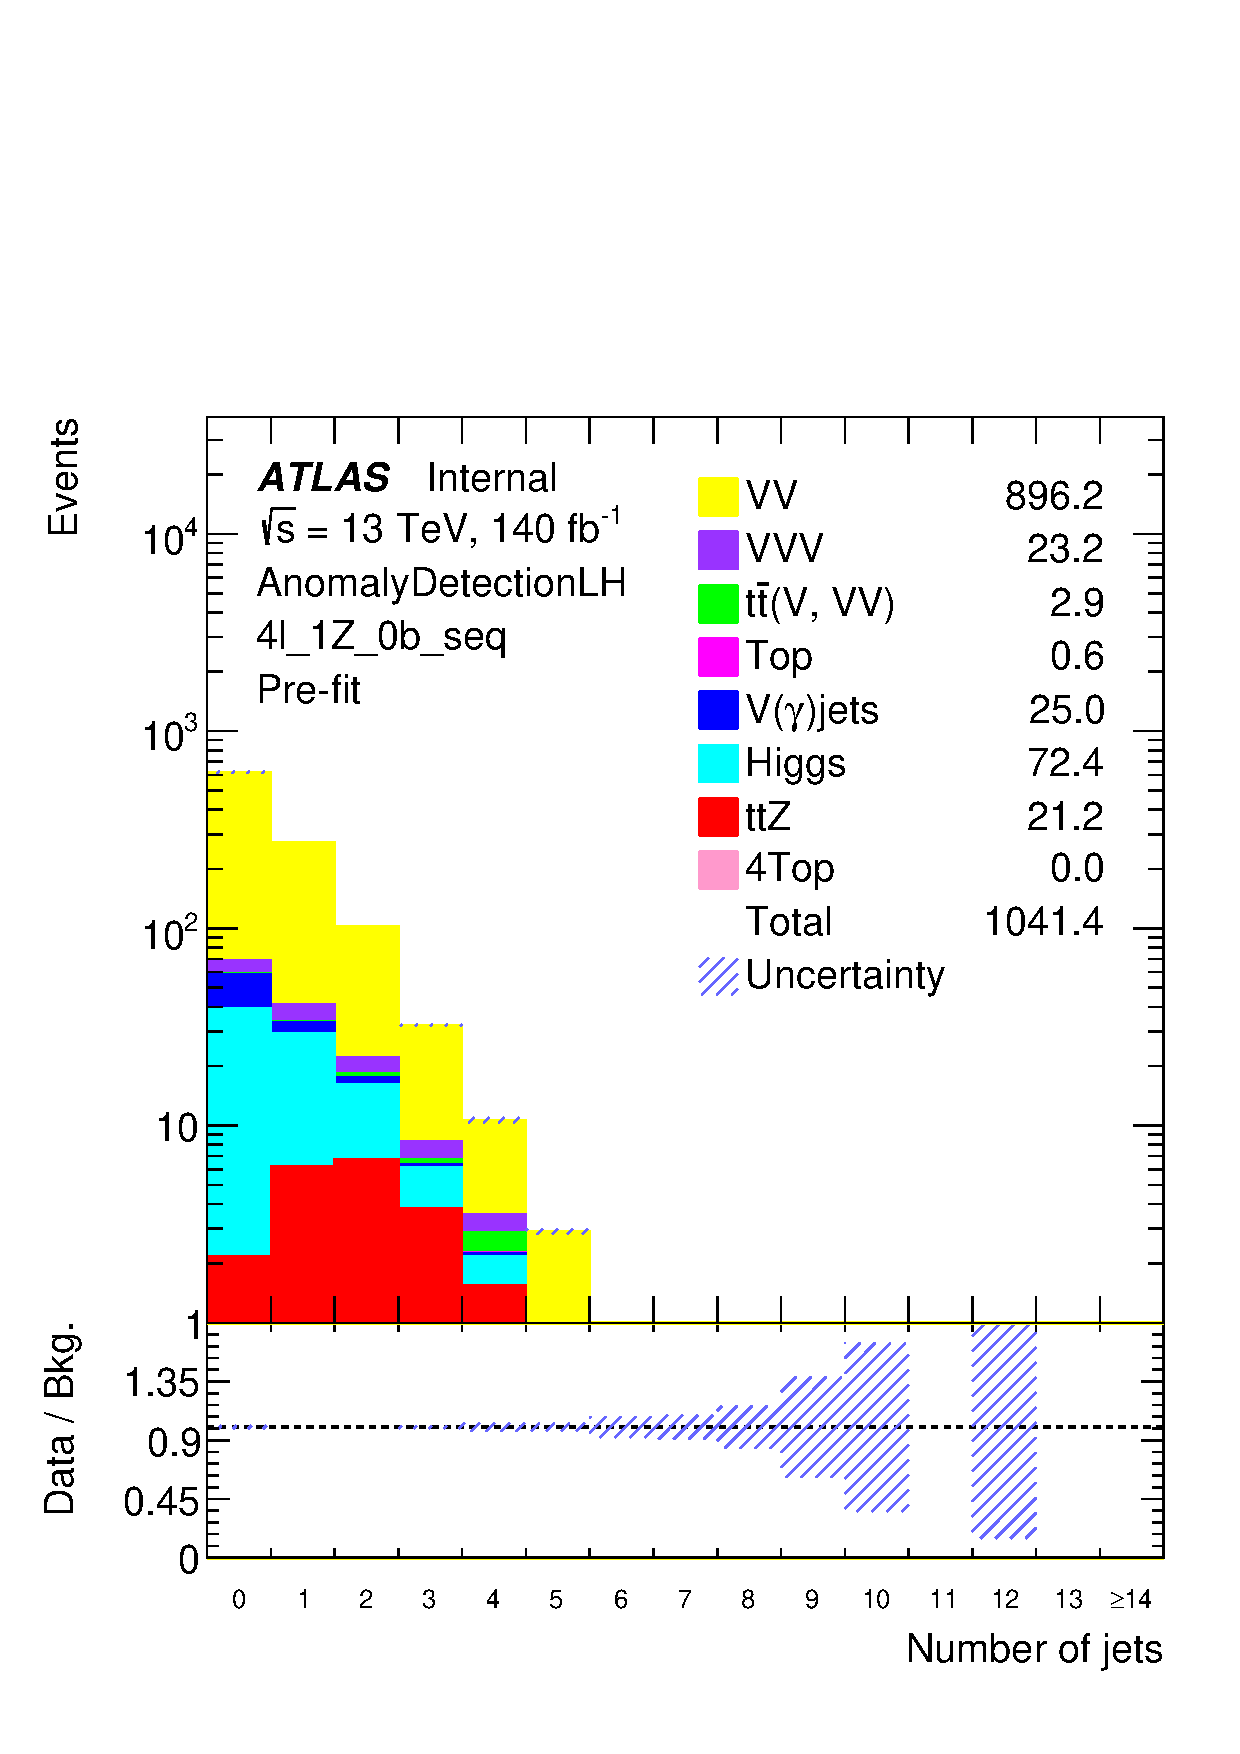
\includegraphics[width=0.24\textwidth]{plots/fourlepLH_run2/Plots/reg_4l_1Z_0b_seq_nJets.pdf} &
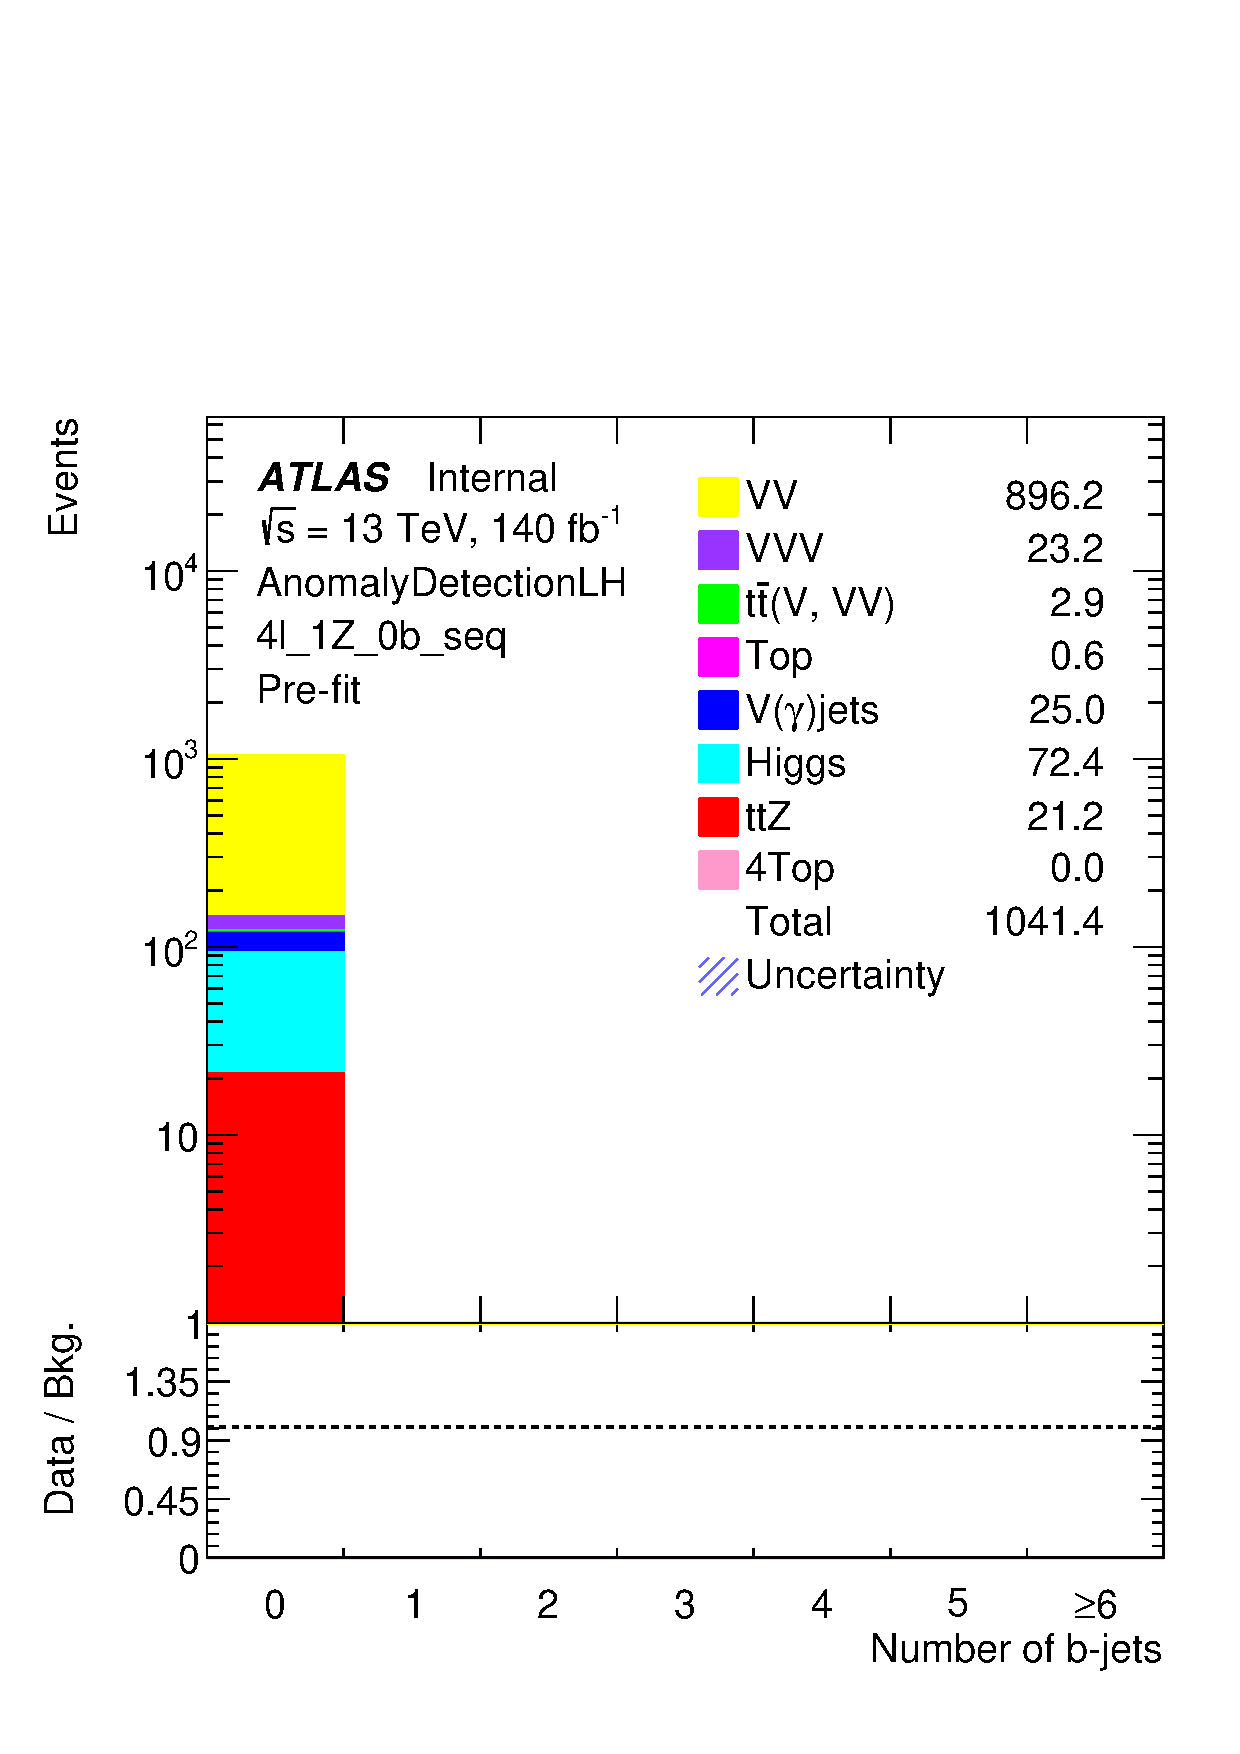
\includegraphics[width=0.24\textwidth]{plots/fourlepLH_run2/Plots/reg_4l_1Z_0b_seq_nbJets.pdf} &
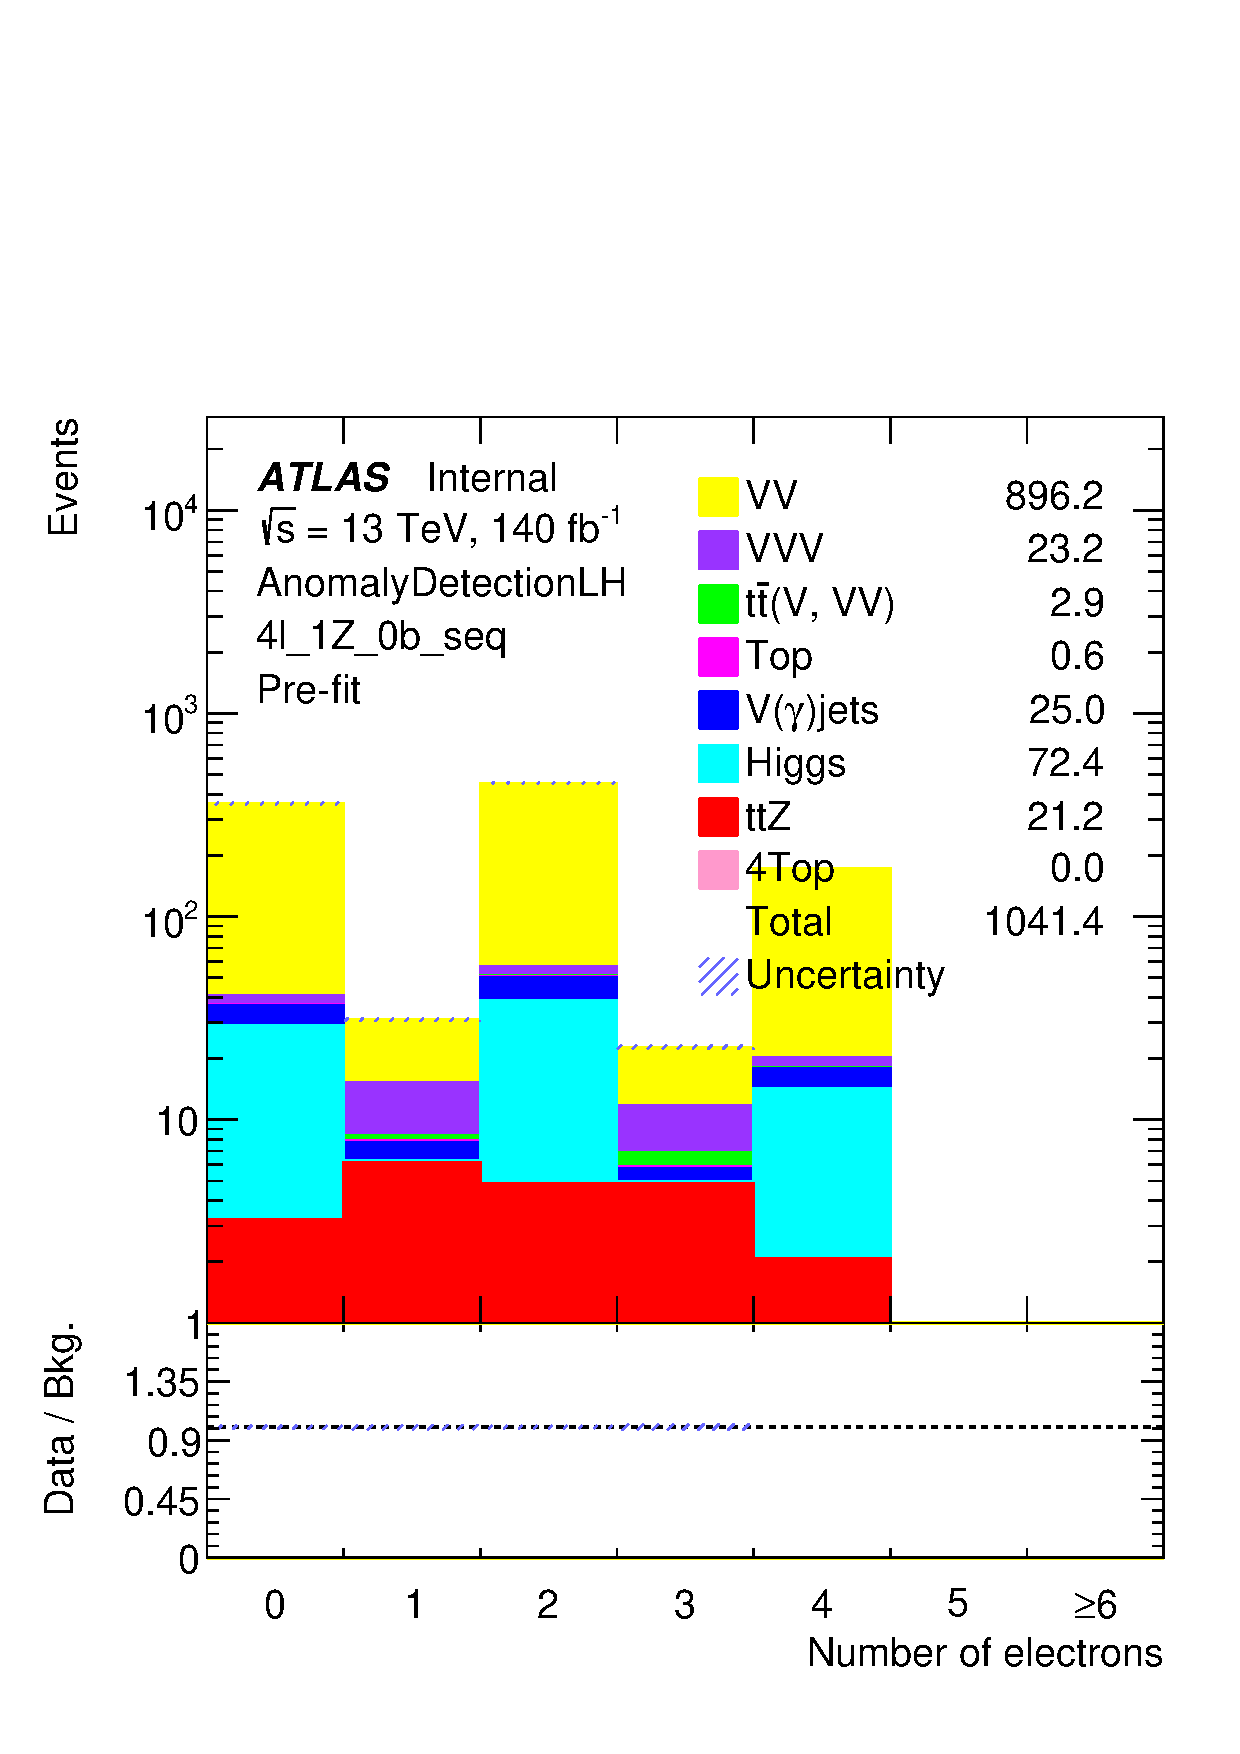
\includegraphics[width=0.24\textwidth]{plots/fourlepLH_run2/Plots/reg_4l_1Z_0b_seq_nElectrons.pdf} &
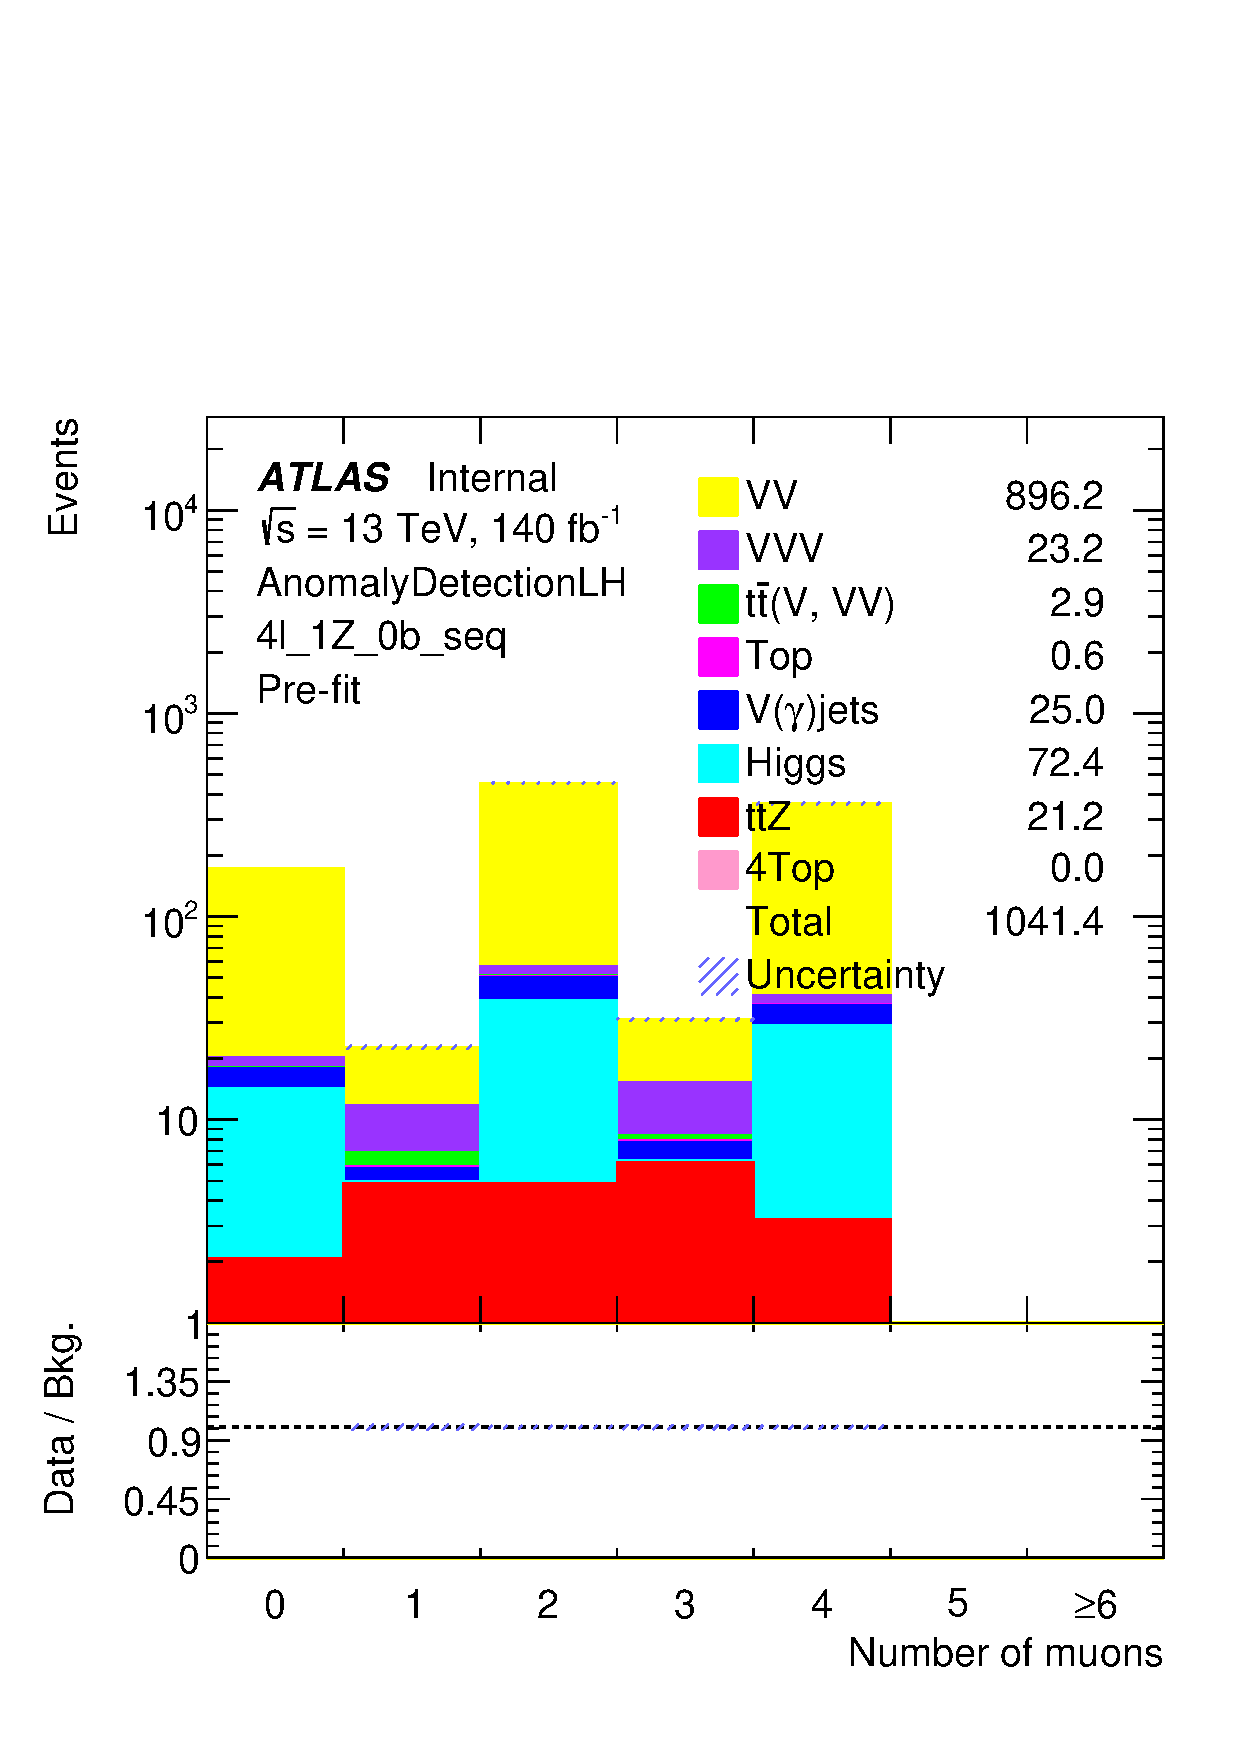
\includegraphics[width=0.24\textwidth]{plots/fourlepLH_run2/Plots/reg_4l_1Z_0b_seq_nMuons.pdf} \\

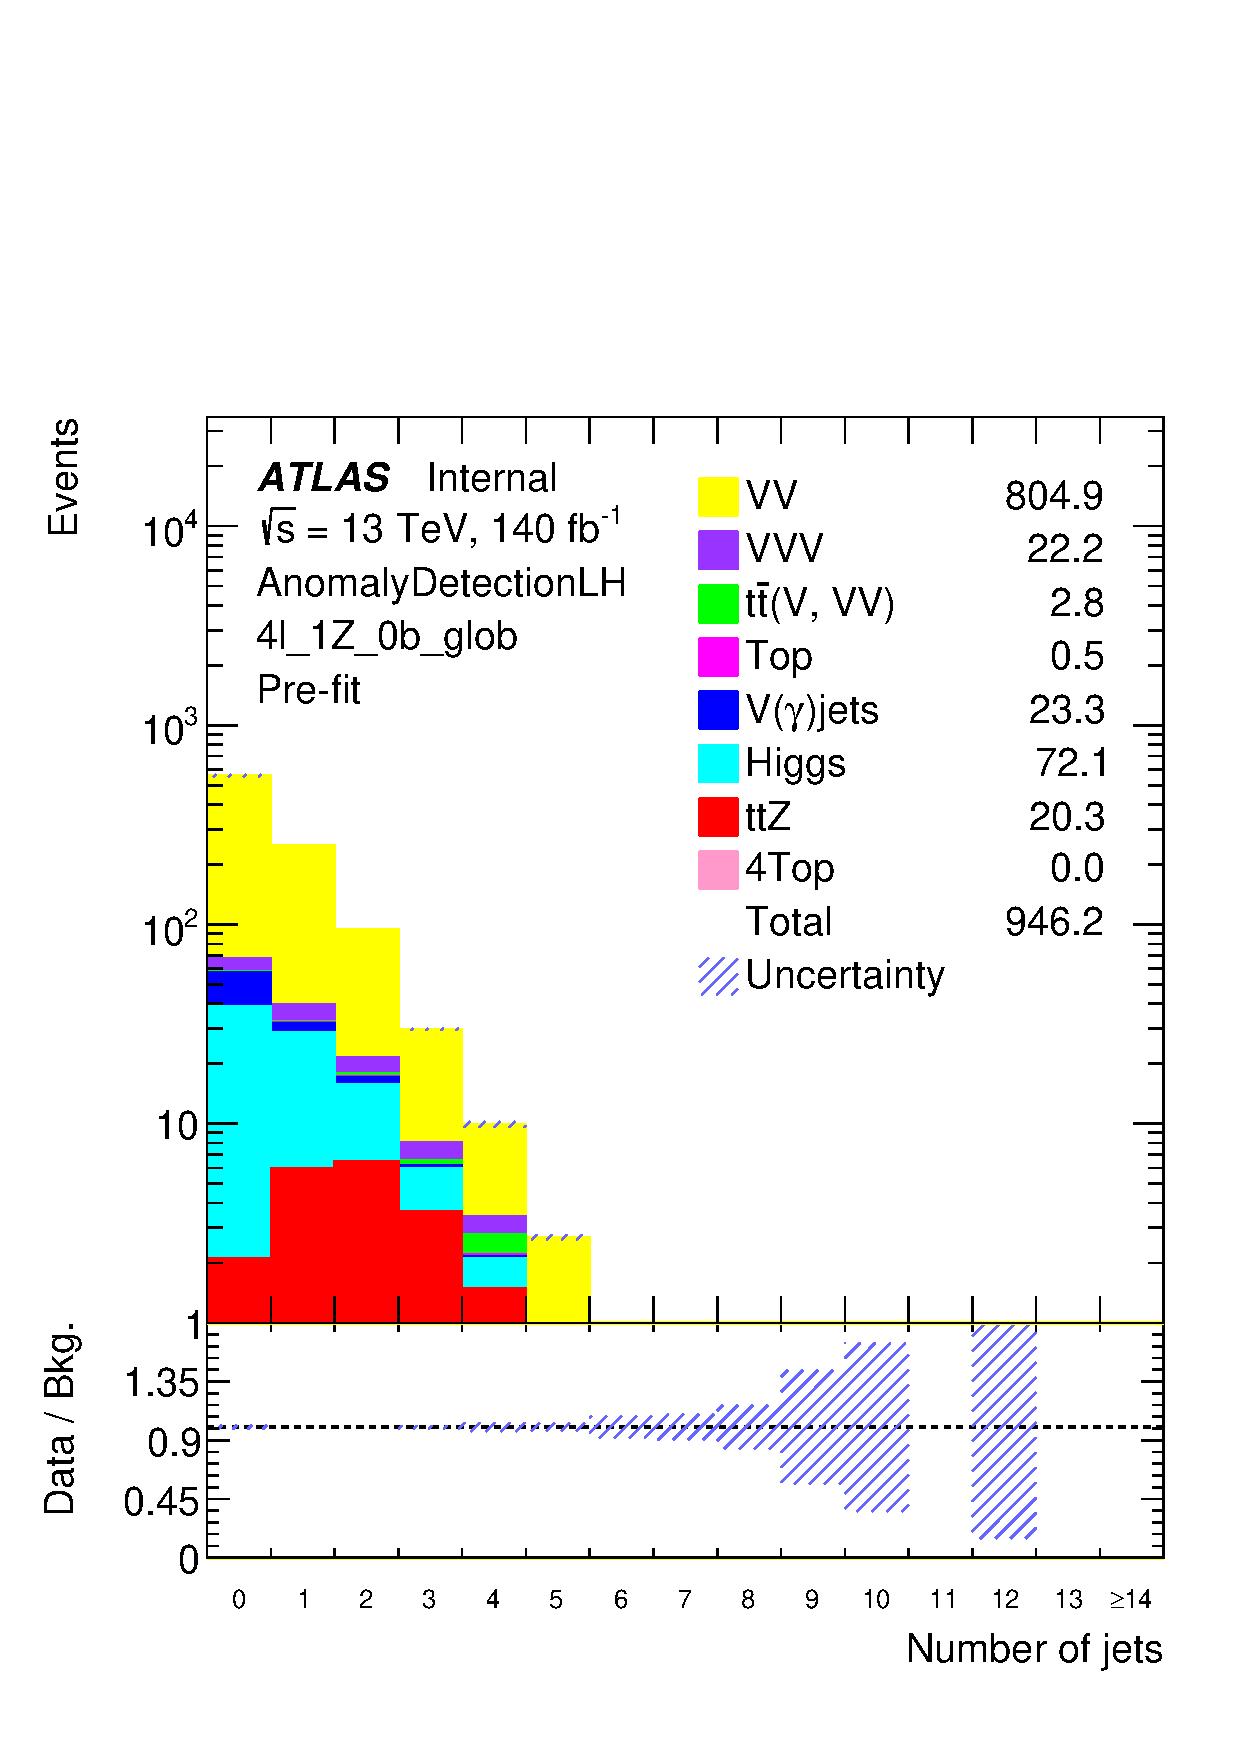
\includegraphics[width=0.24\textwidth]{plots/fourlepLH_run2/Plots/reg_4l_1Z_0b_glob_nJets.pdf} &
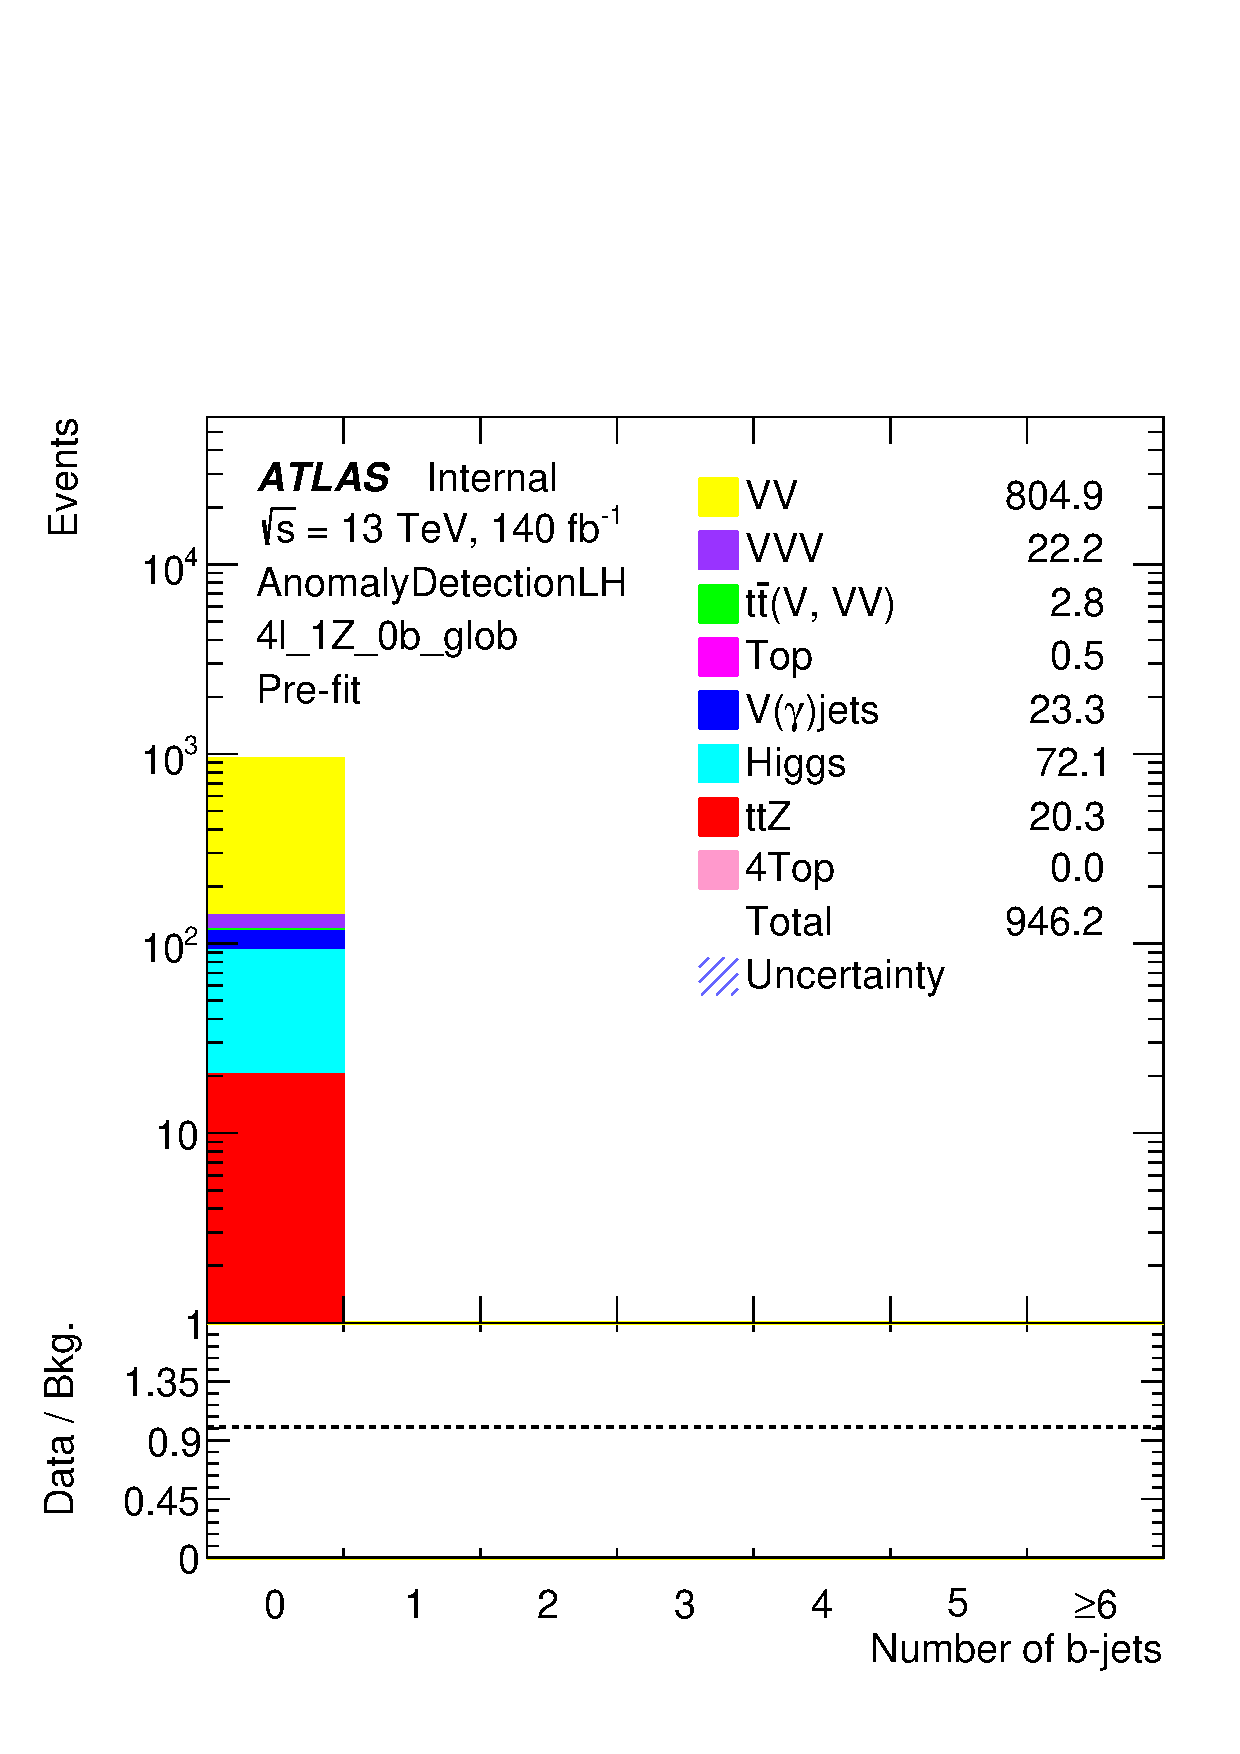
\includegraphics[width=0.24\textwidth]{plots/fourlepLH_run2/Plots/reg_4l_1Z_0b_glob_nbJets.pdf} &
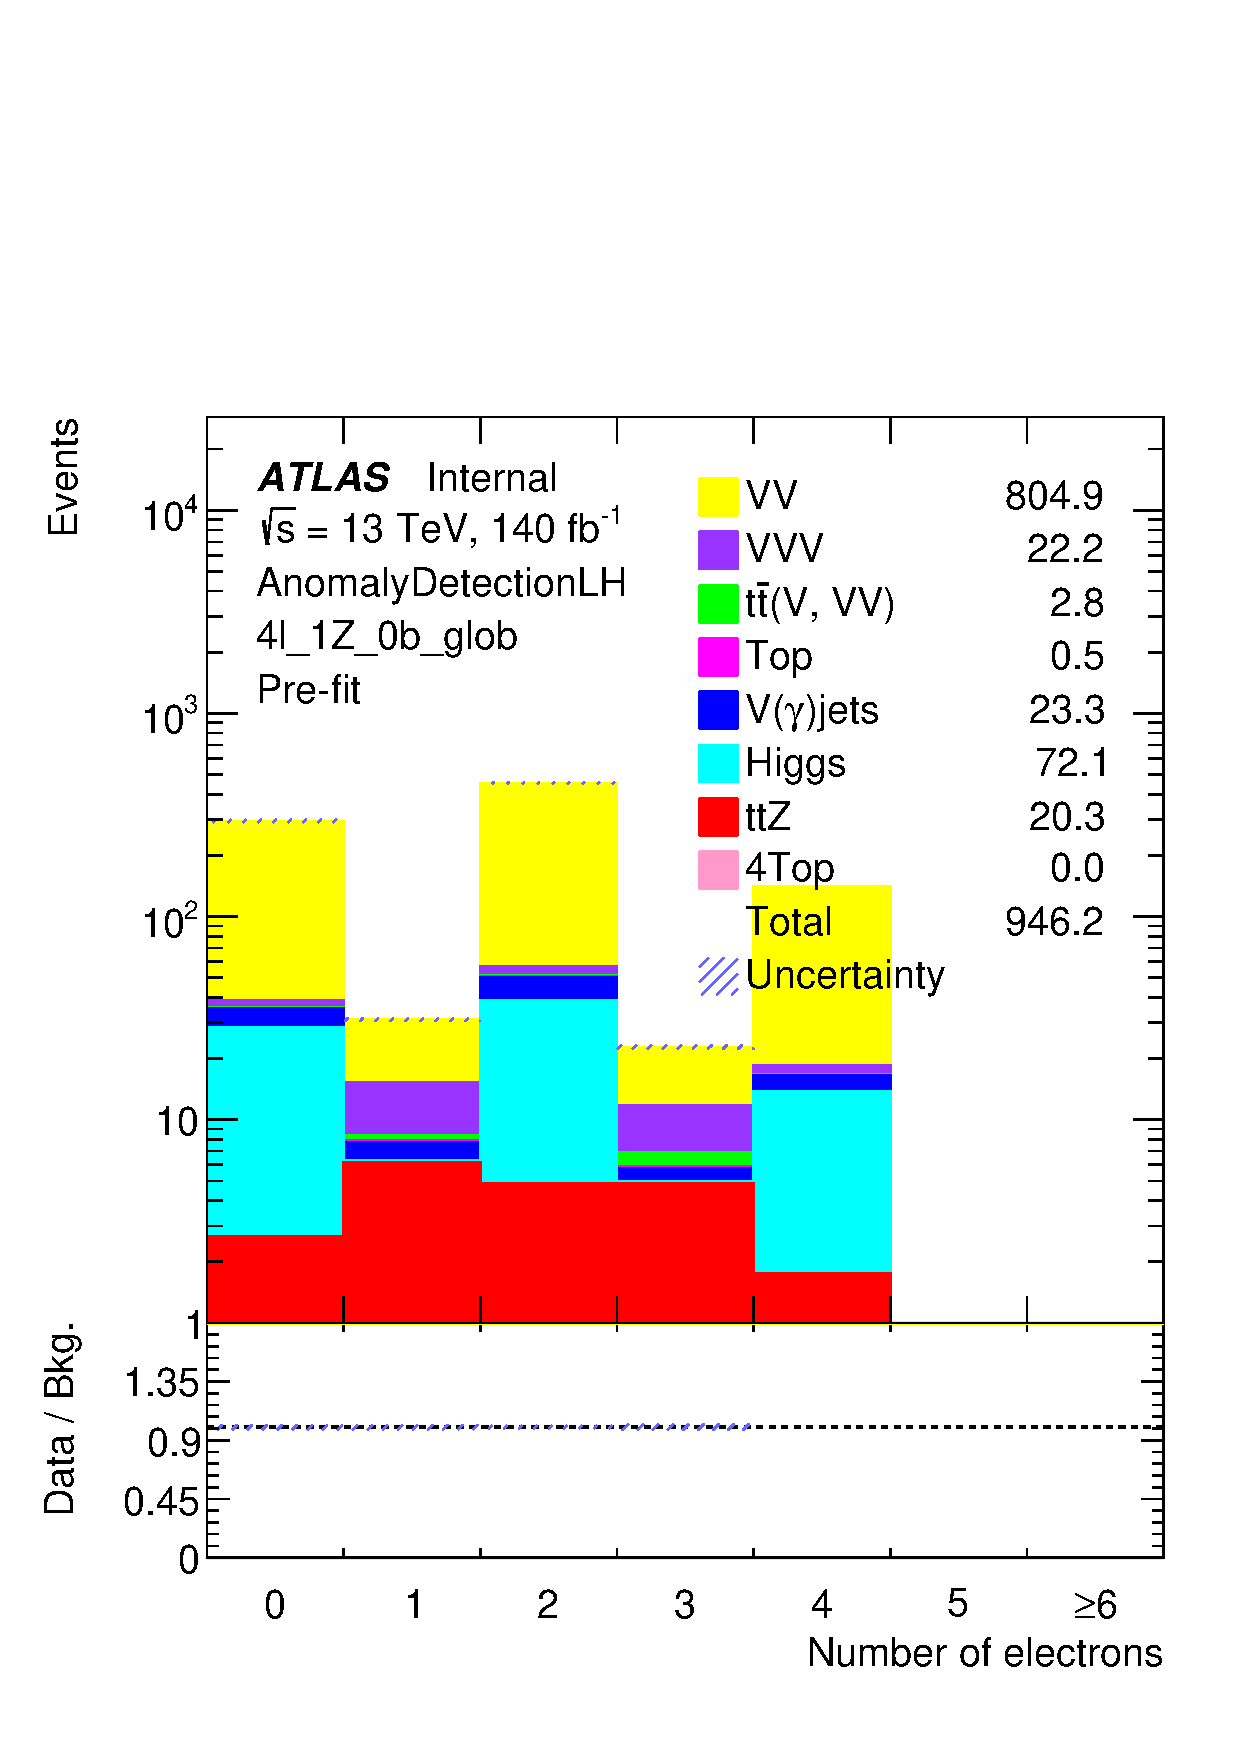
\includegraphics[width=0.24\textwidth]{plots/fourlepLH_run2/Plots/reg_4l_1Z_0b_glob_nElectrons.pdf} &
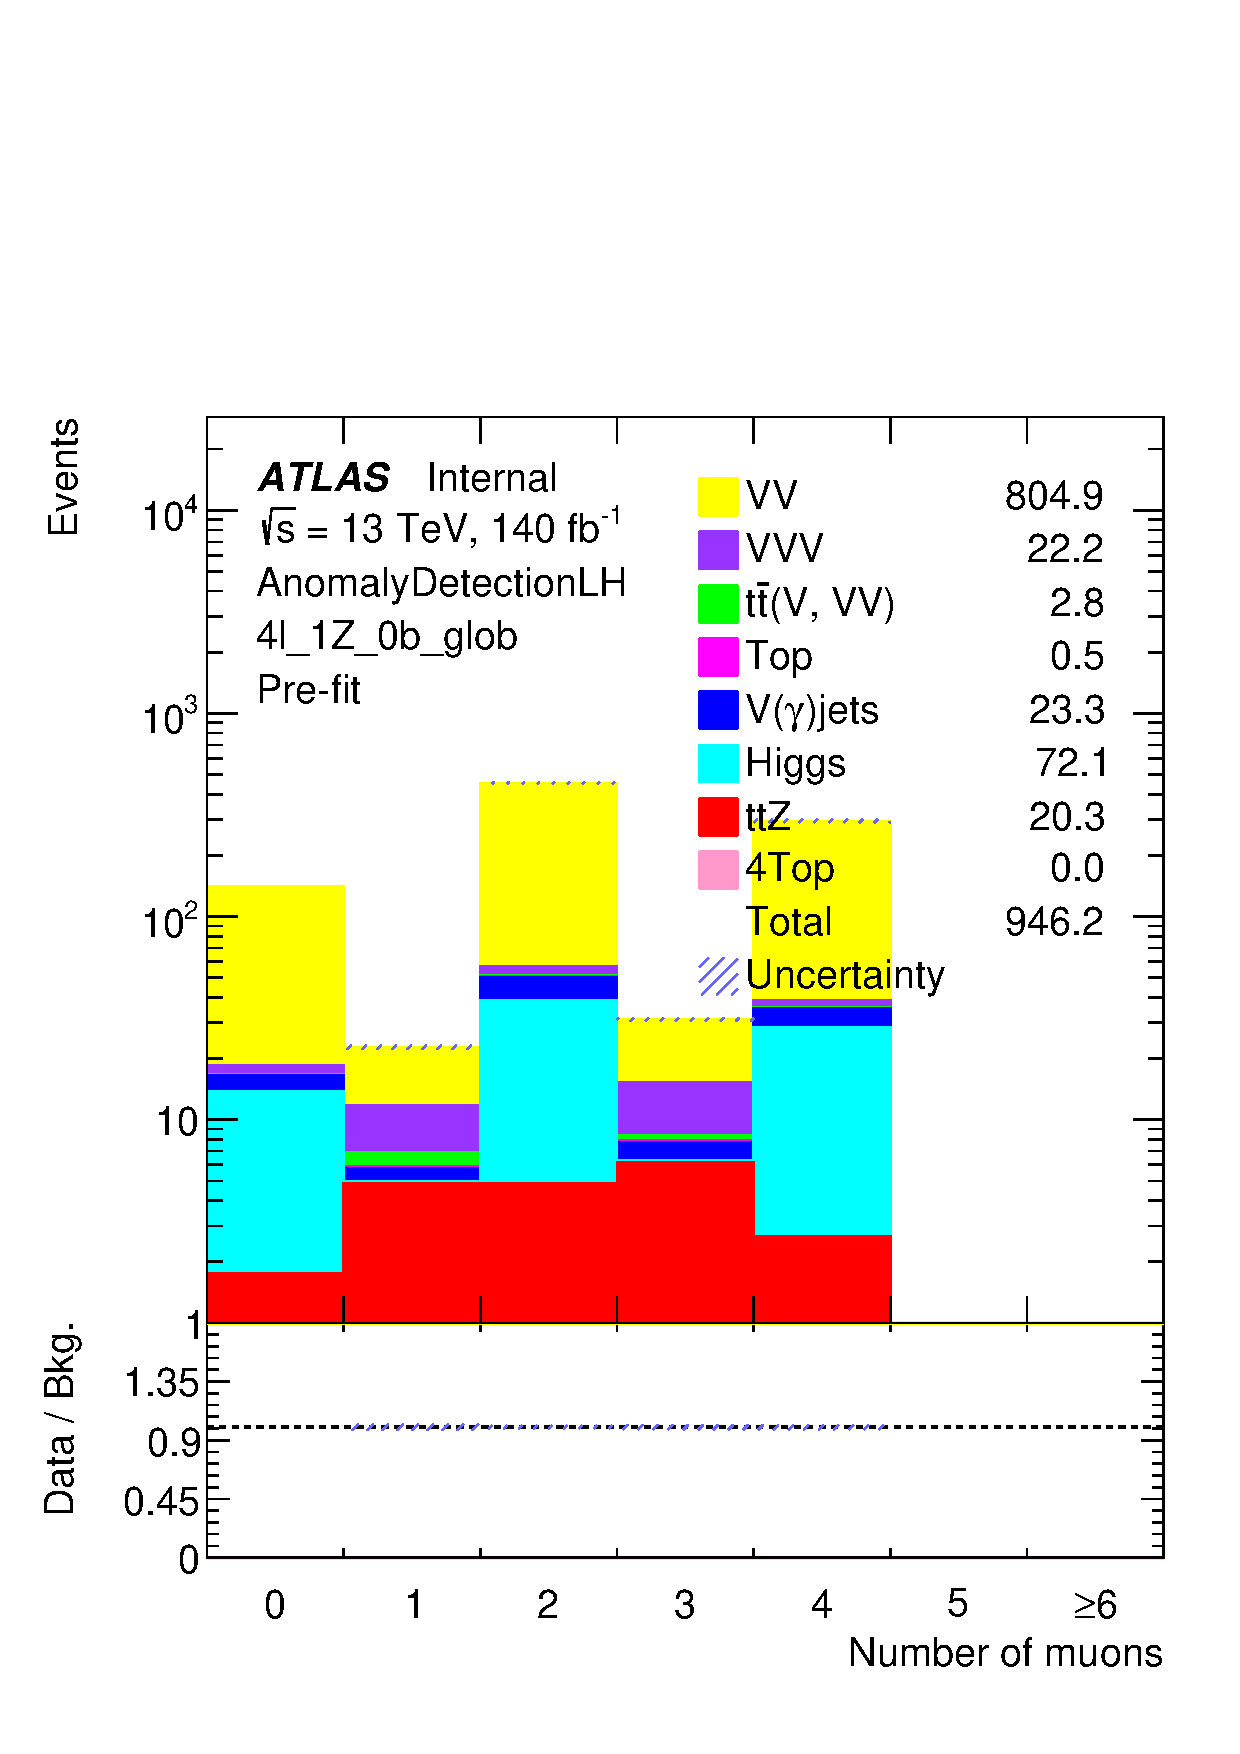
\includegraphics[width=0.24\textwidth]{plots/fourlepLH_run2/Plots/reg_4l_1Z_0b_glob_nMuons.pdf} \\

\end{tabular}
\end{frame}

\begin{frame}{\texttt{Results: 4l\_1Z\_0b}}
\begin{tabular}{cccccc}
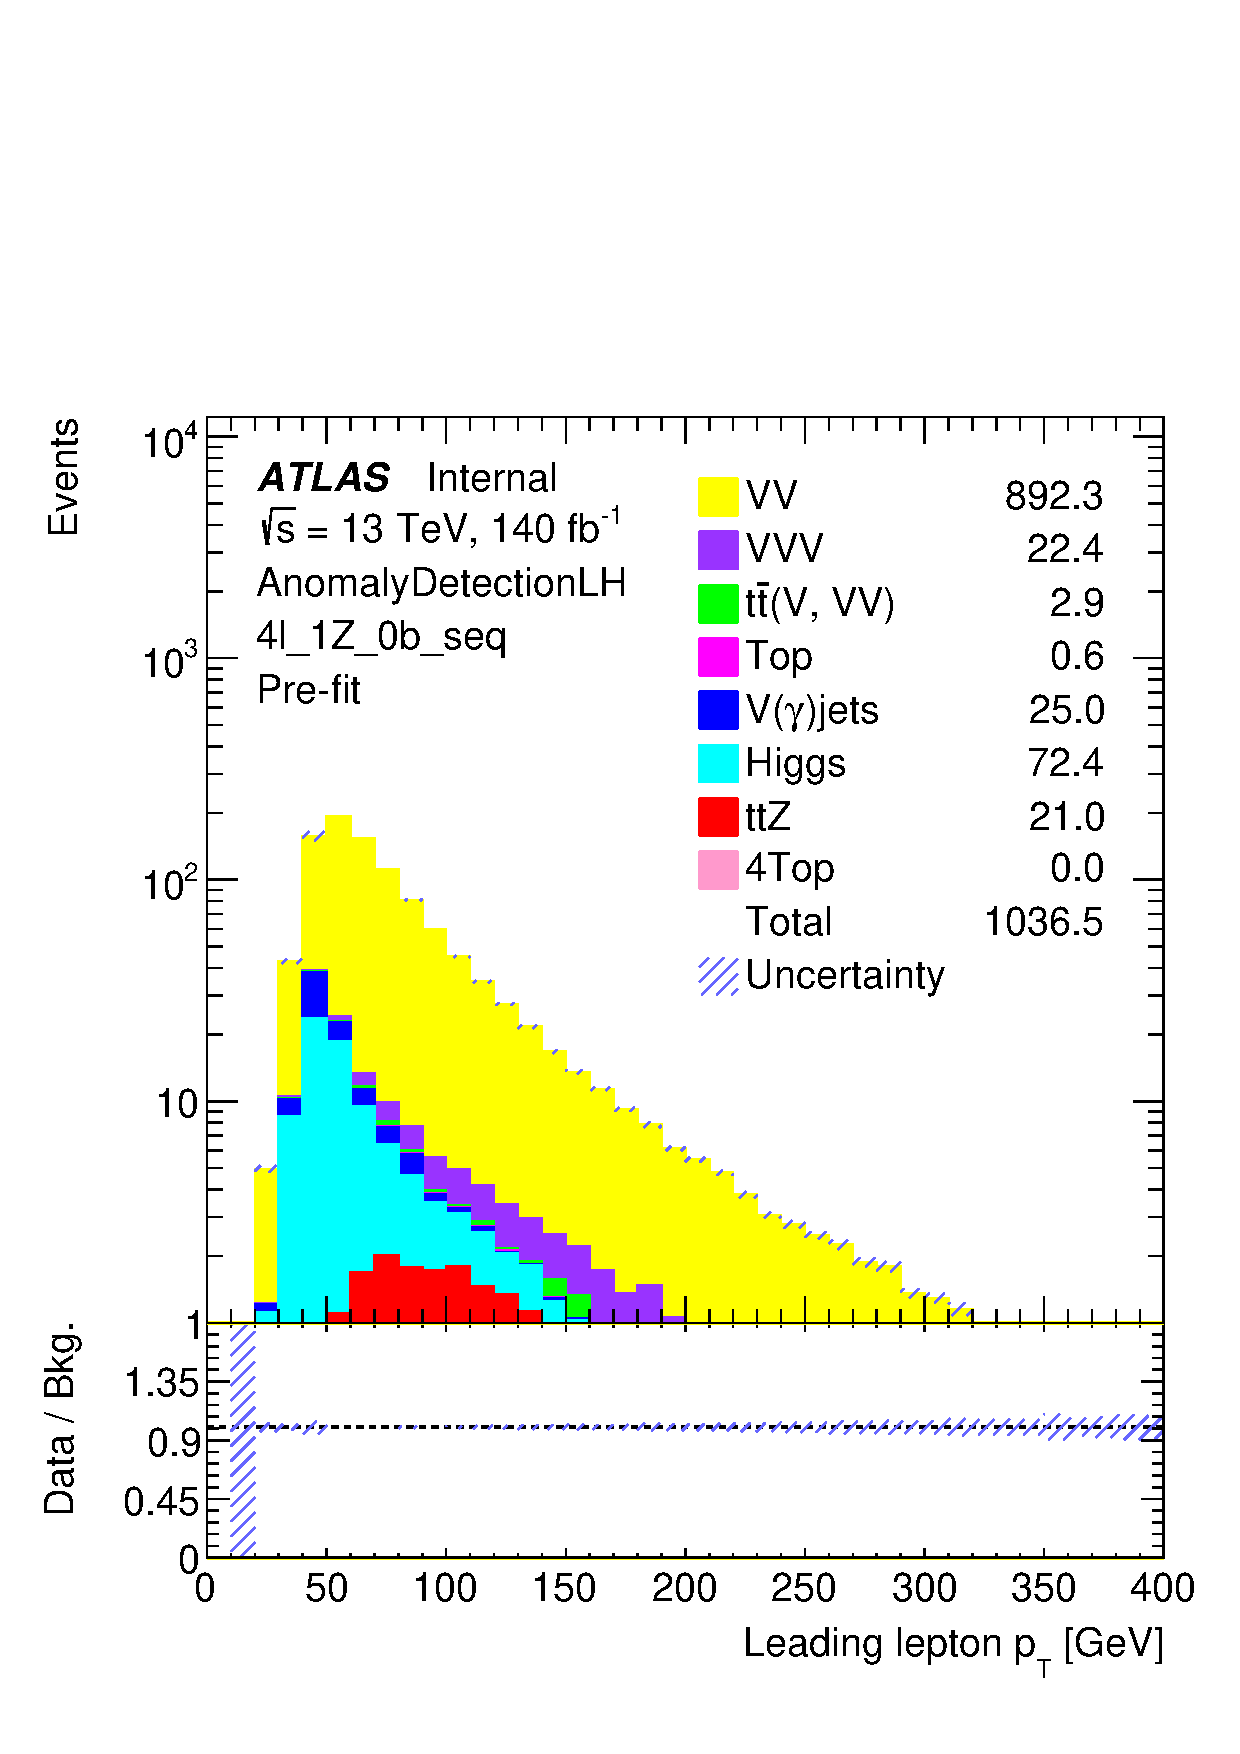
\includegraphics[width=0.24\textwidth]{plots/fourlepLH_run2/Plots/reg_4l_1Z_0b_seq_lep_pt_0.pdf} &
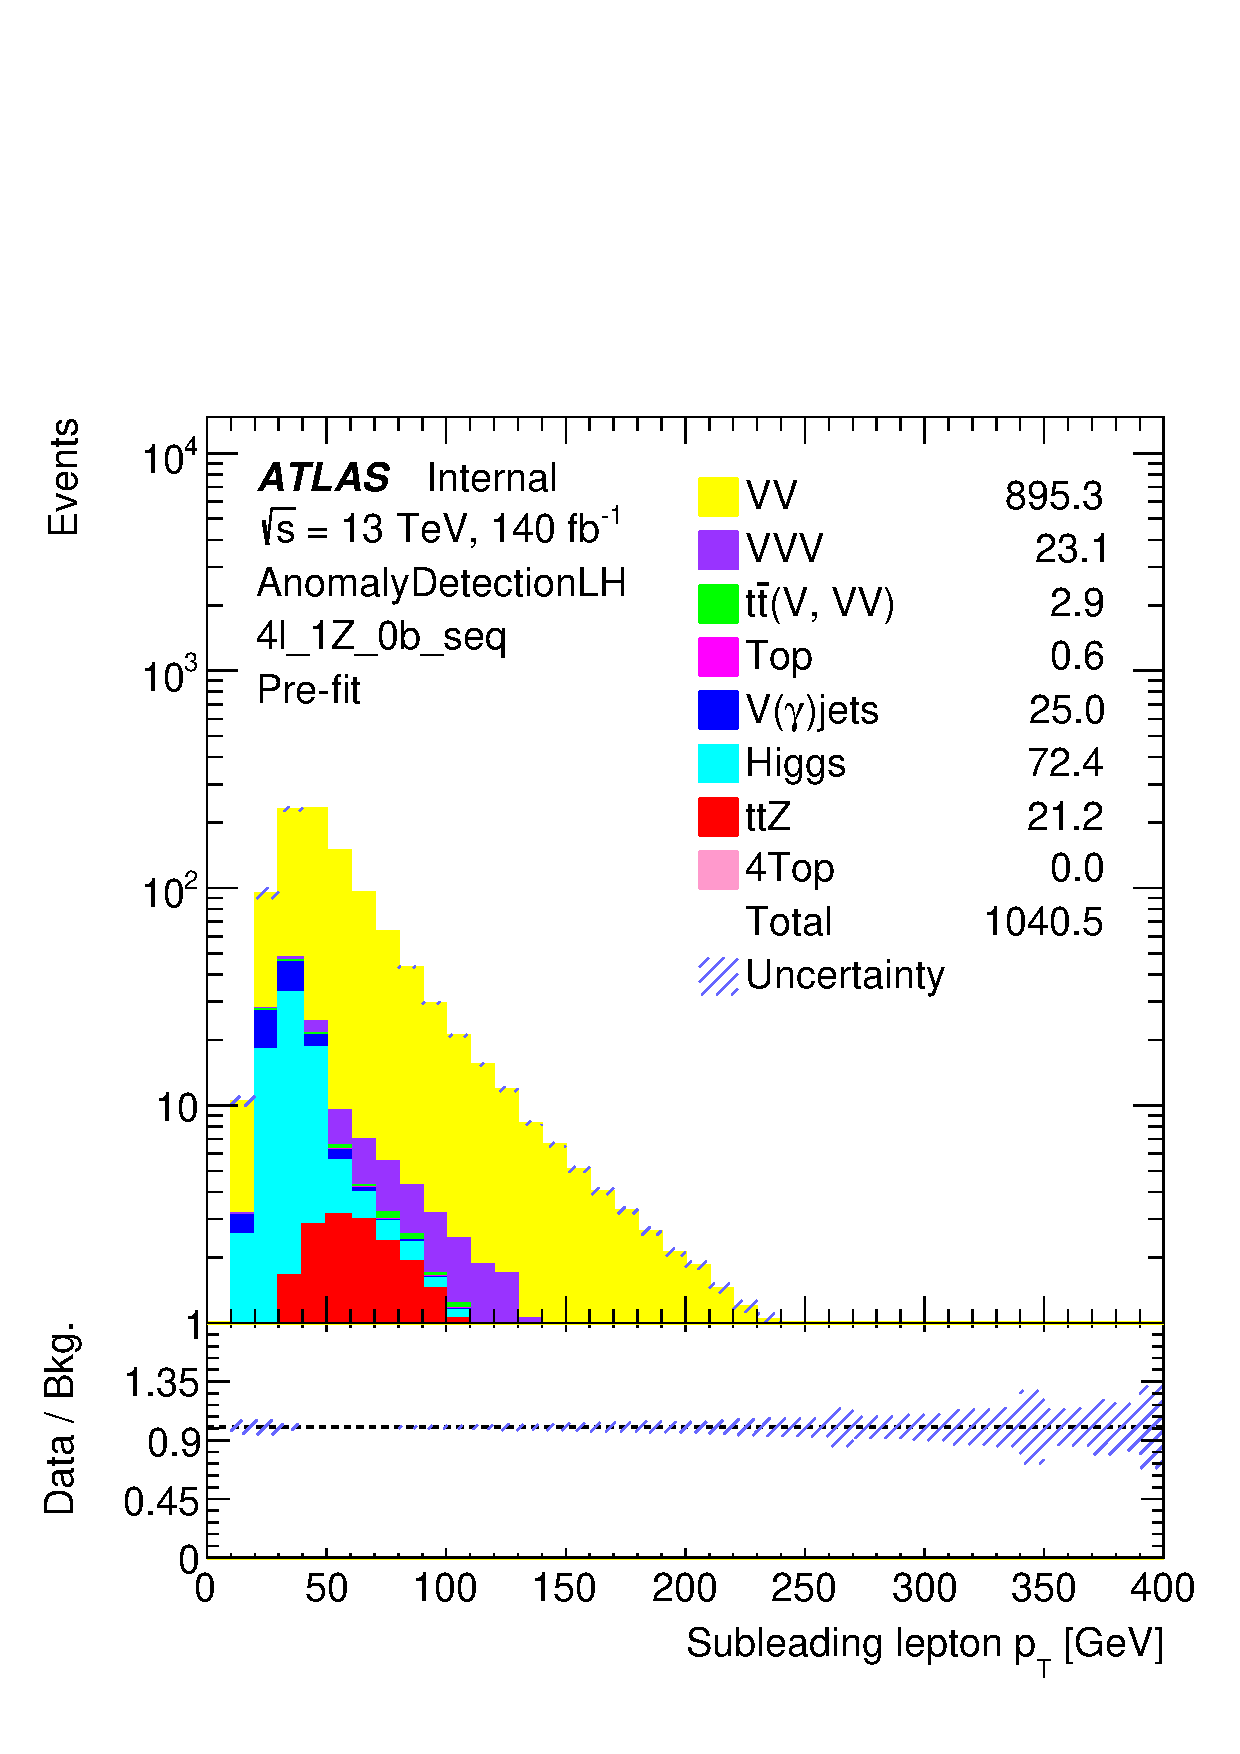
\includegraphics[width=0.24\textwidth]{plots/fourlepLH_run2/Plots/reg_4l_1Z_0b_seq_lep_pt_1.pdf} &
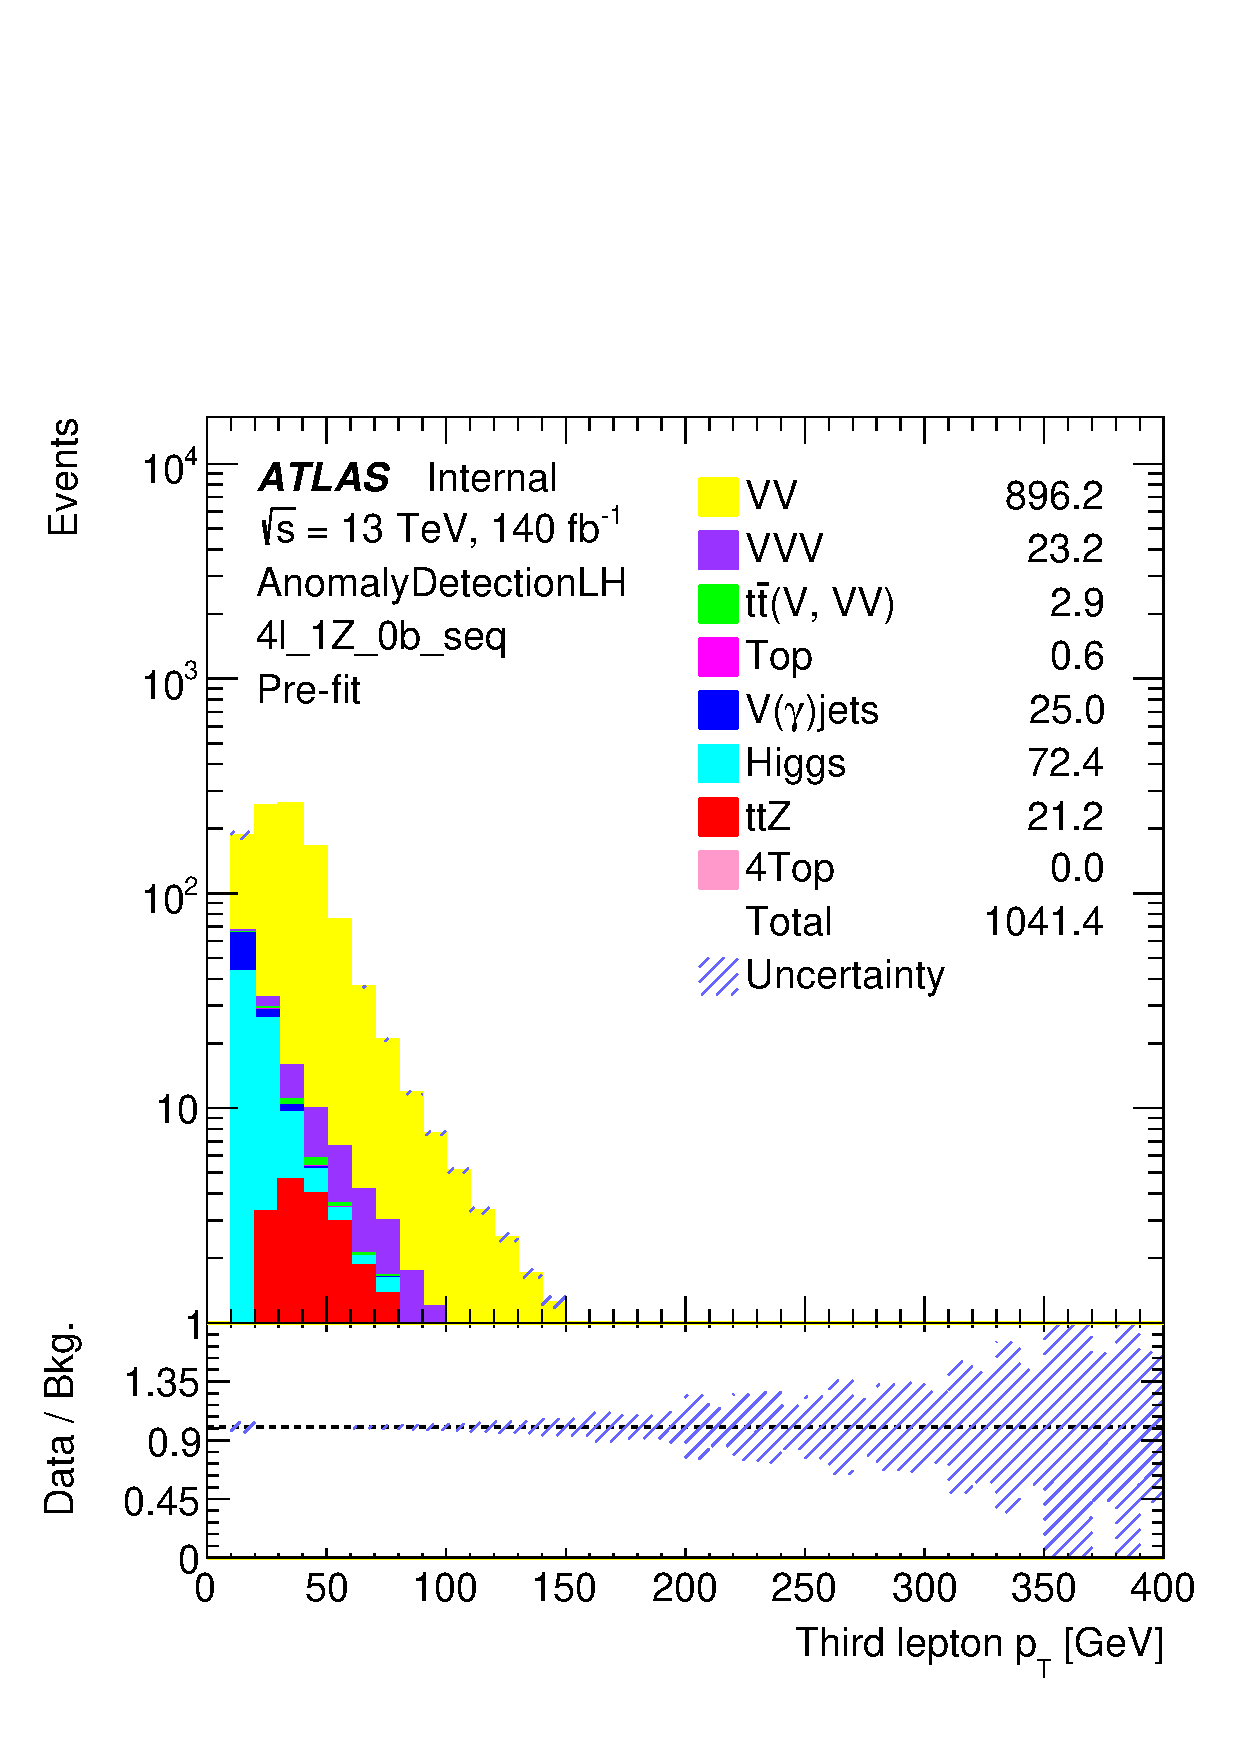
\includegraphics[width=0.24\textwidth]{plots/fourlepLH_run2/Plots/reg_4l_1Z_0b_seq_lep_pt_2.pdf} &
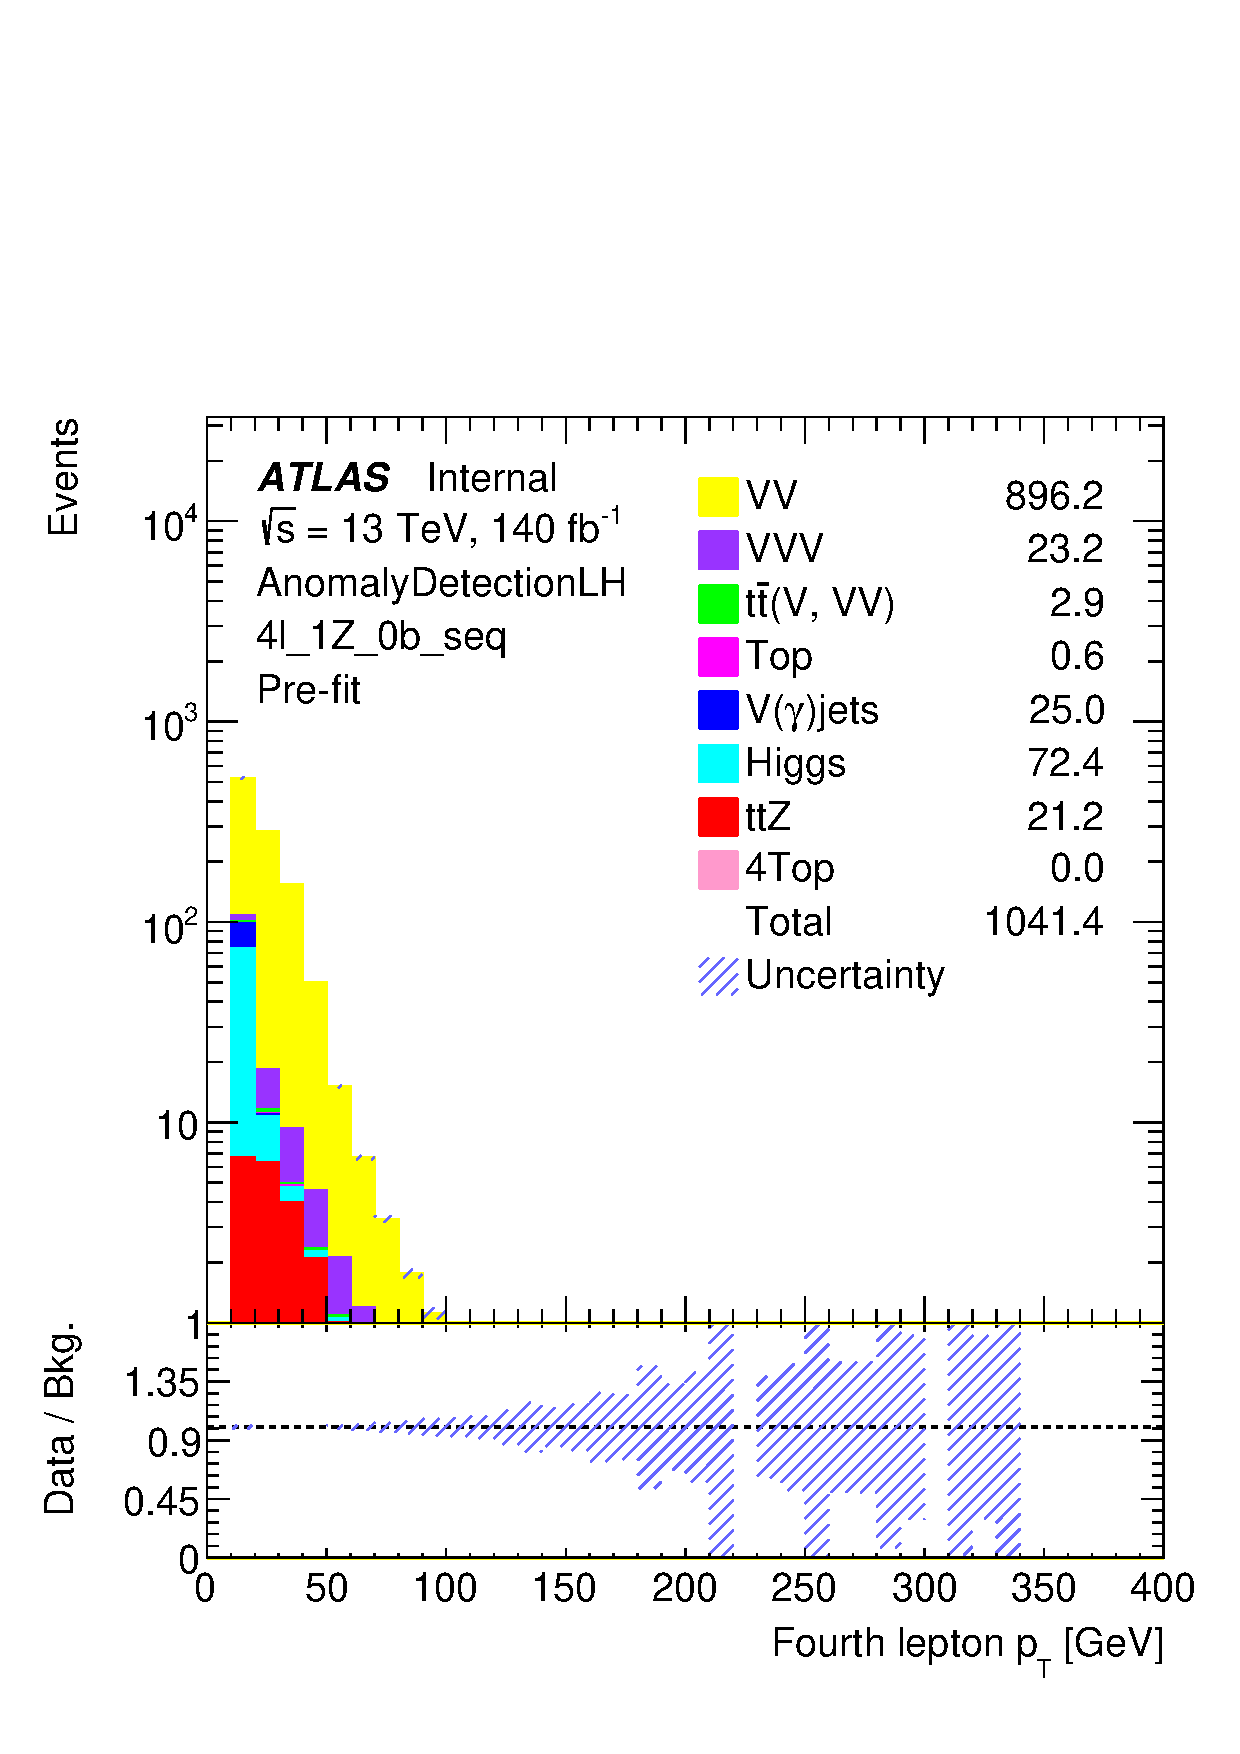
\includegraphics[width=0.24\textwidth]{plots/fourlepLH_run2/Plots/reg_4l_1Z_0b_seq_lep_pt_3.pdf} \\

\includegraphics[width=0.24\textwidth]{plots/fourlepLH_run2/Plots/reg_4l_1Z_0b_glob_lep_pt_0.pdf} &
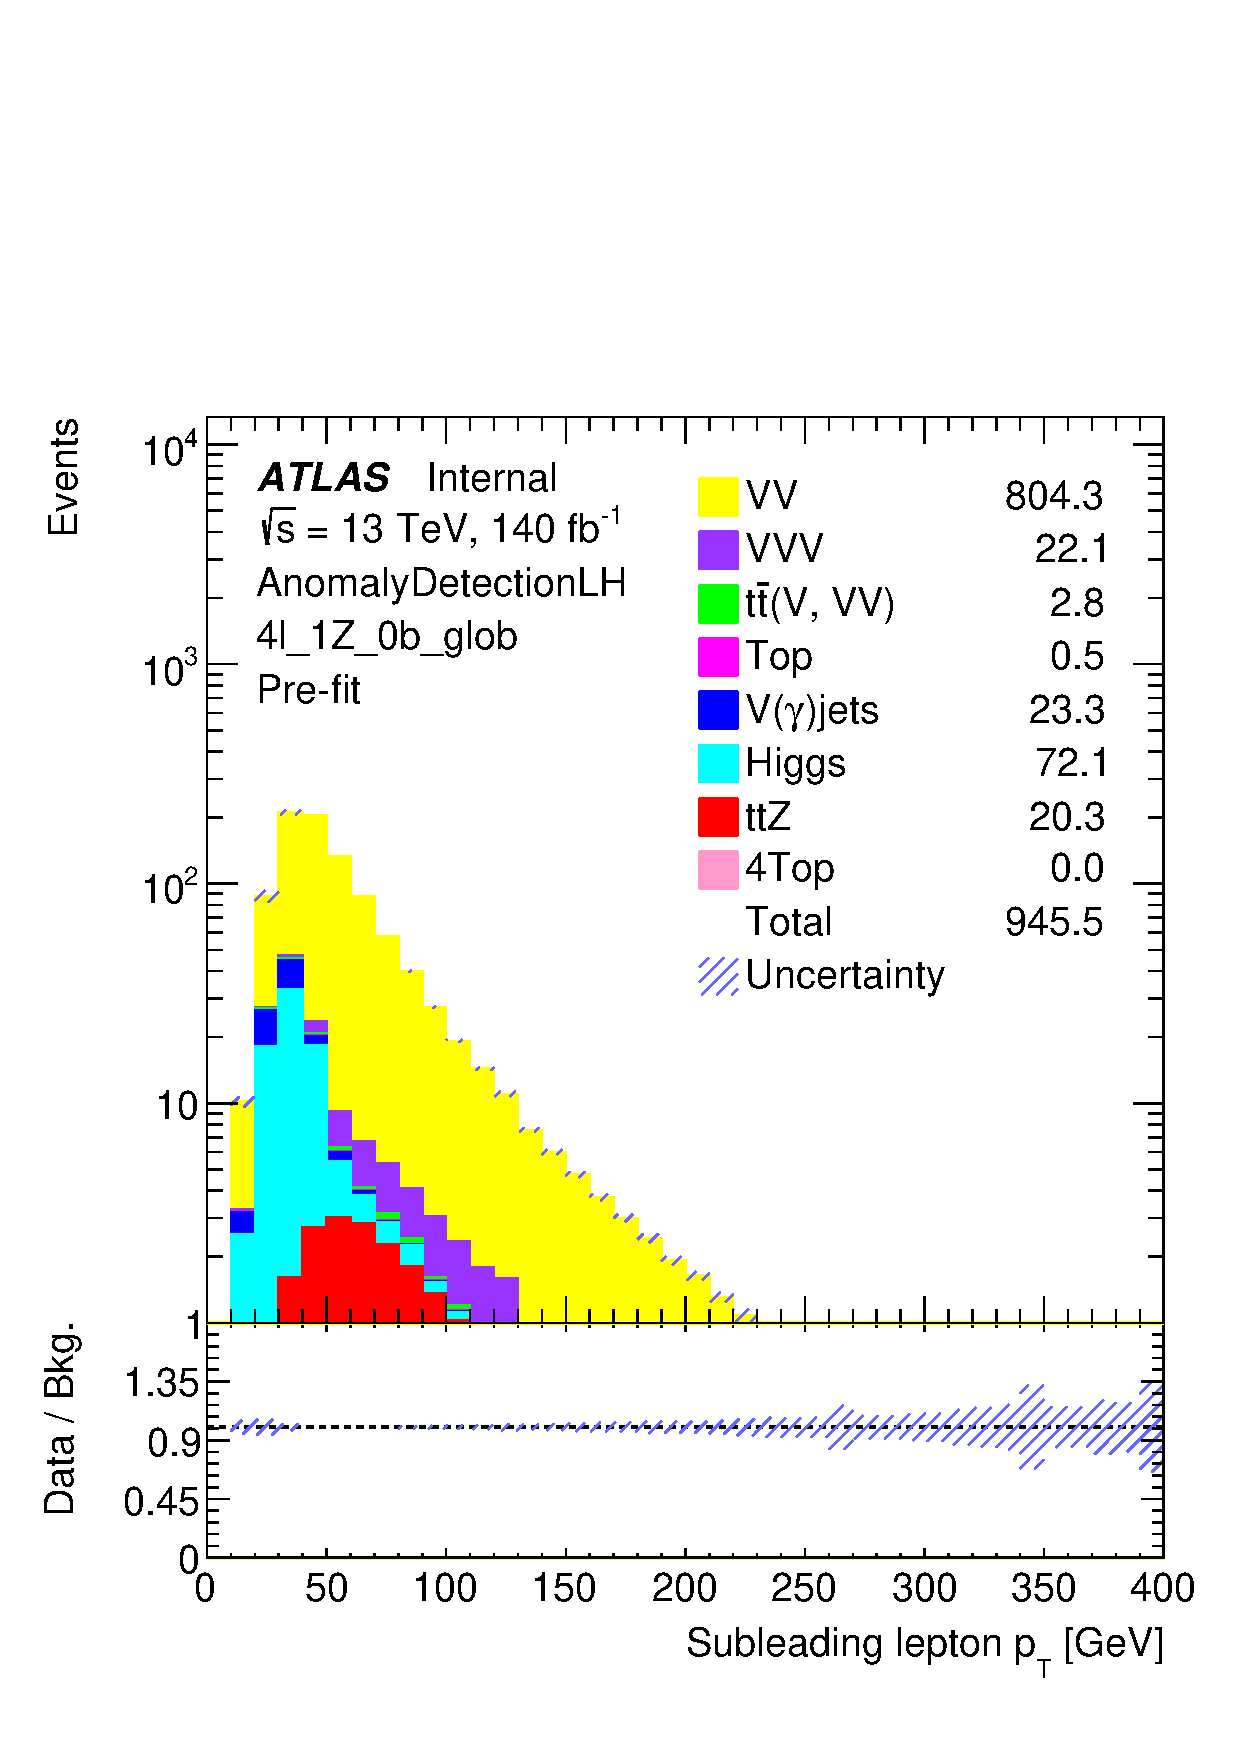
\includegraphics[width=0.24\textwidth]{plots/fourlepLH_run2/Plots/reg_4l_1Z_0b_glob_lep_pt_1.pdf} &
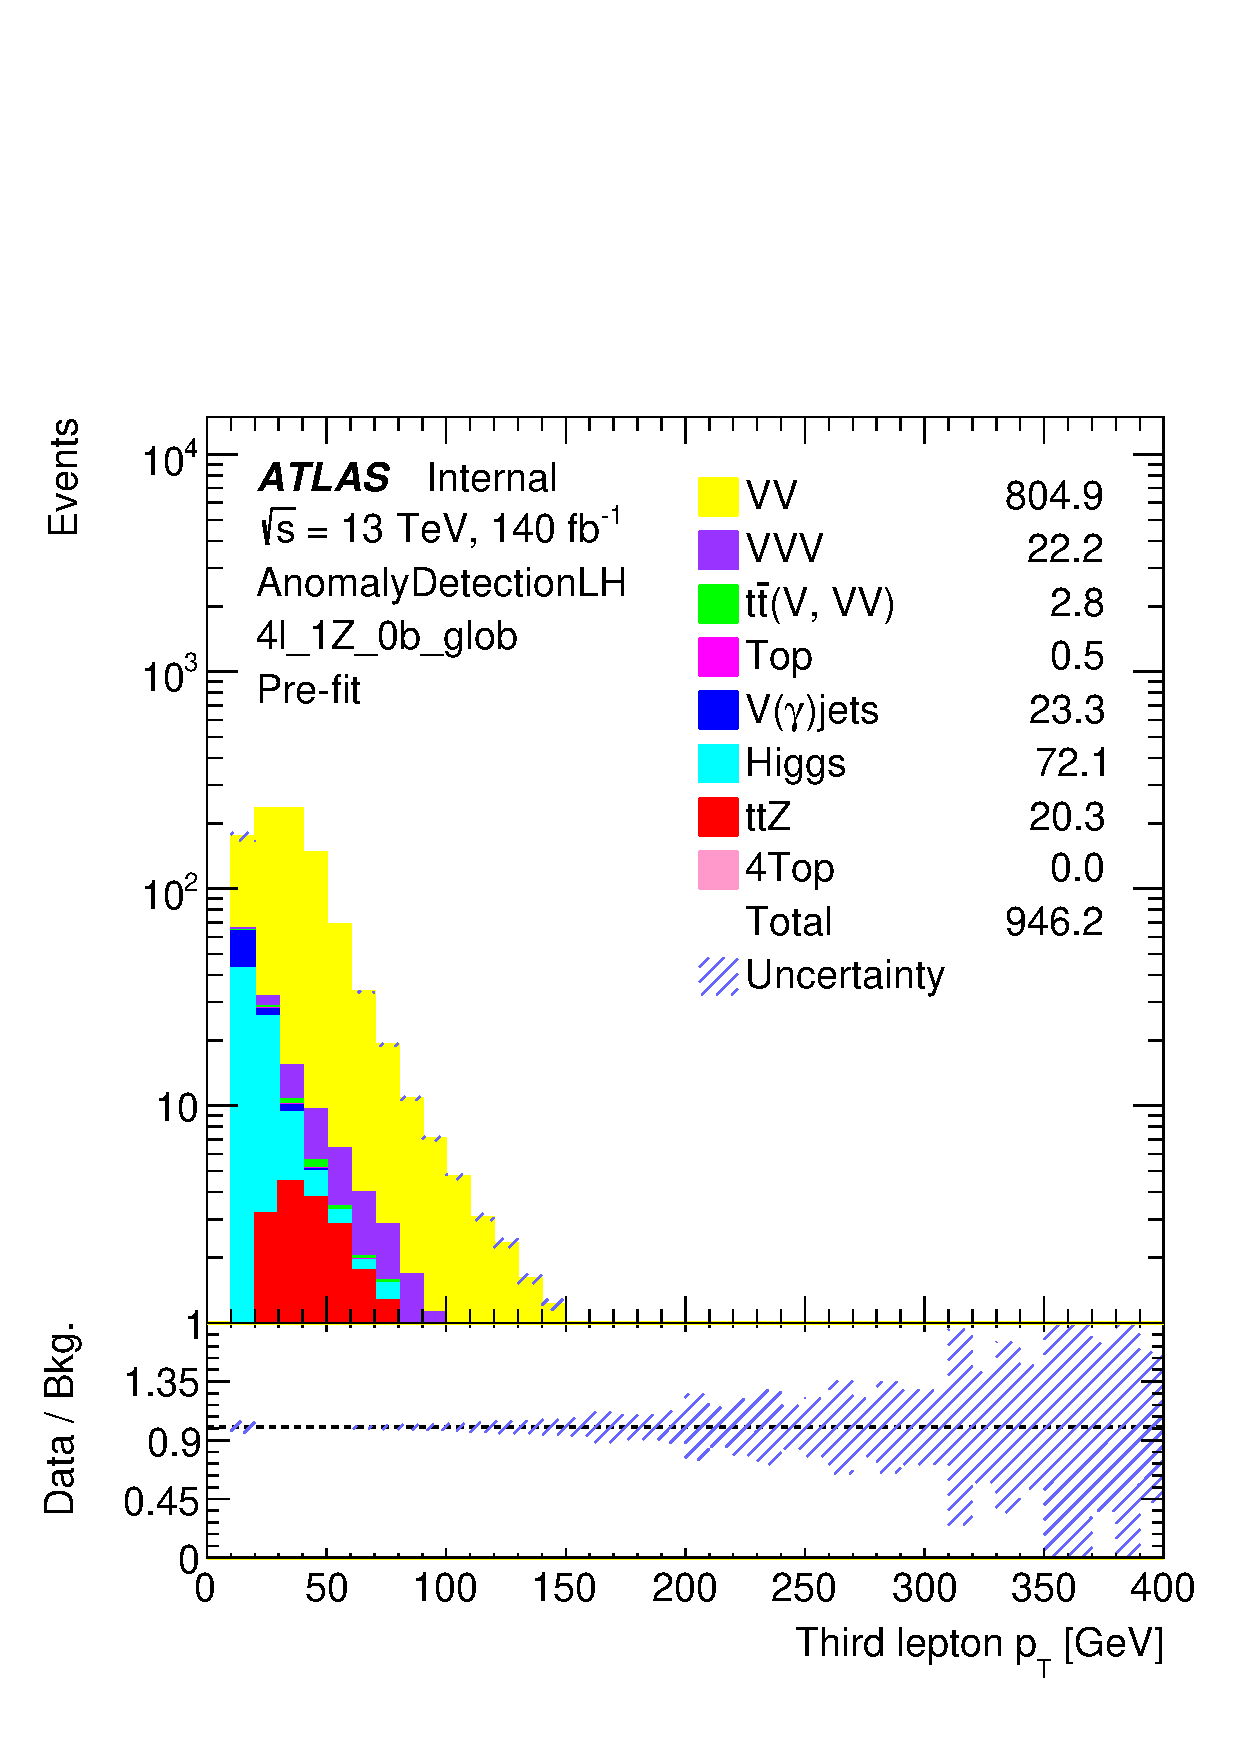
\includegraphics[width=0.24\textwidth]{plots/fourlepLH_run2/Plots/reg_4l_1Z_0b_glob_lep_pt_2.pdf} &
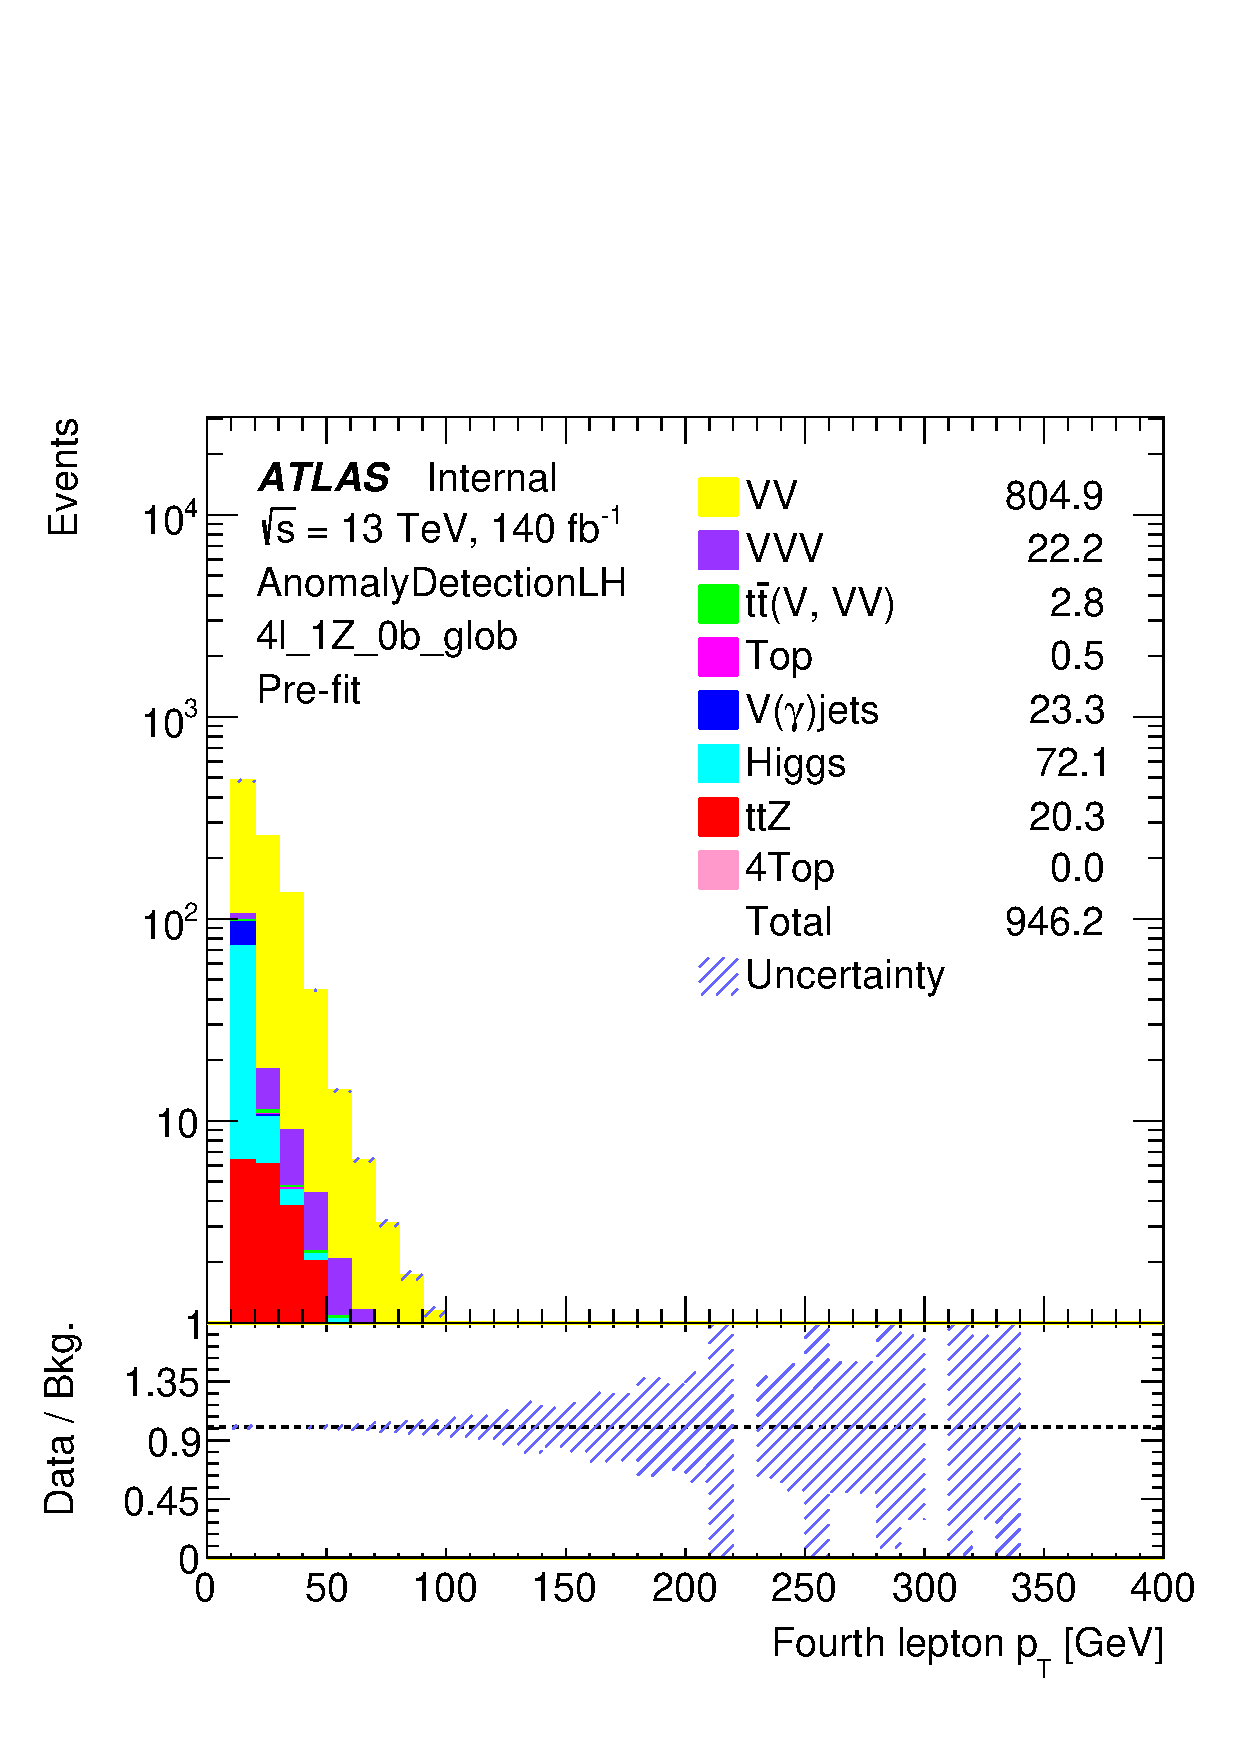
\includegraphics[width=0.24\textwidth]{plots/fourlepLH_run2/Plots/reg_4l_1Z_0b_glob_lep_pt_3.pdf} \\

\end{tabular}

\end{frame}
\subsection{4l\_1Z\_1b}
\begin{frame}{\texttt{Focused selection: 4l\_1Z\_1b}}
%\tiny
\centering
\begin{tabular}{|c|c|}
\hline

4l\_1Z\_1b\_seq &
4l\_1Z\_1b\_glob \\
\hline
\multicolumn{2}{|c|}{\texttt{globalTriggerMatchSLTorDLT\_LooseLH\_custTrig\_NOSYS}} \\
\multicolumn{2}{|c|}{\texttt{pass\_fourlep\_LooseLH\_NOSYS} }\\
\multicolumn{2}{|c|}{\texttt{$N_{leptons}$=4}} \\
\multicolumn{2}{|c|}{\texttt{$N_{taus}$ $\geq 0$} } \\
\multicolumn{2}{|c|}{$N_{b\mathrm{-jets}}$ $\geq 1$} \\
\multicolumn{2}{|c|}{\texttt{Q = 0}} \\

\hline

\texttt{$|m_{Z1}^{seq}-91.2e3| < 10e3$} &
\texttt{$|m_{Z1}^{glob}-91.2e3| < 10e3$} &\\
\texttt{$|m_{Z2}^{seq}-91.2e3| < 10e3$} &
\texttt{$|m_{Z2}^{glob}-91.2e3| < 10e3$}\\

\hline

\end{tabular}
\end{frame}

\begin{frame}{\texttt{Results: 4l\_1Z\_1b}}
\centering
\begin{tabular}{cccccc}

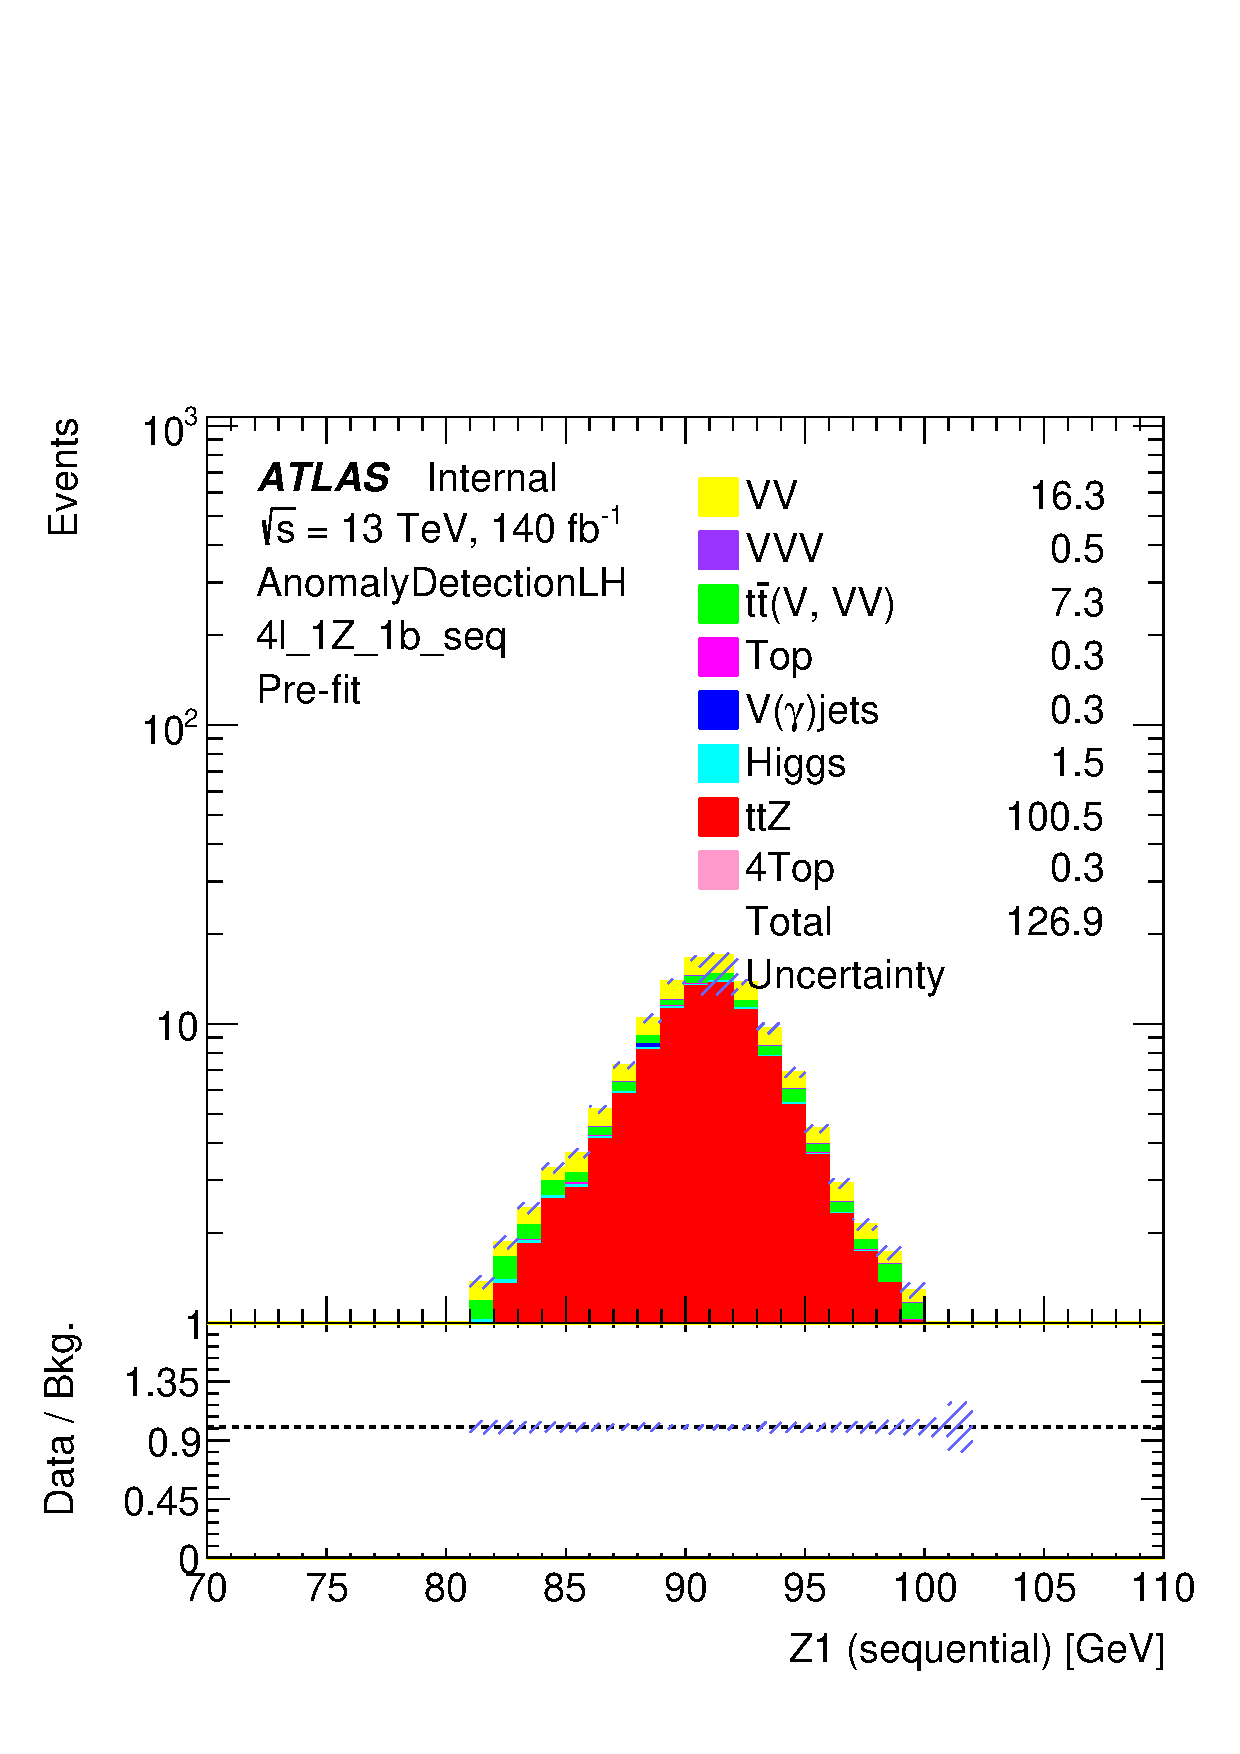
\includegraphics[width=0.24\textwidth]{plots/fourlepLH_run2/Plots/reg_4l_1Z_1b_seq_Z1_mass_seq_1GeV.pdf} &
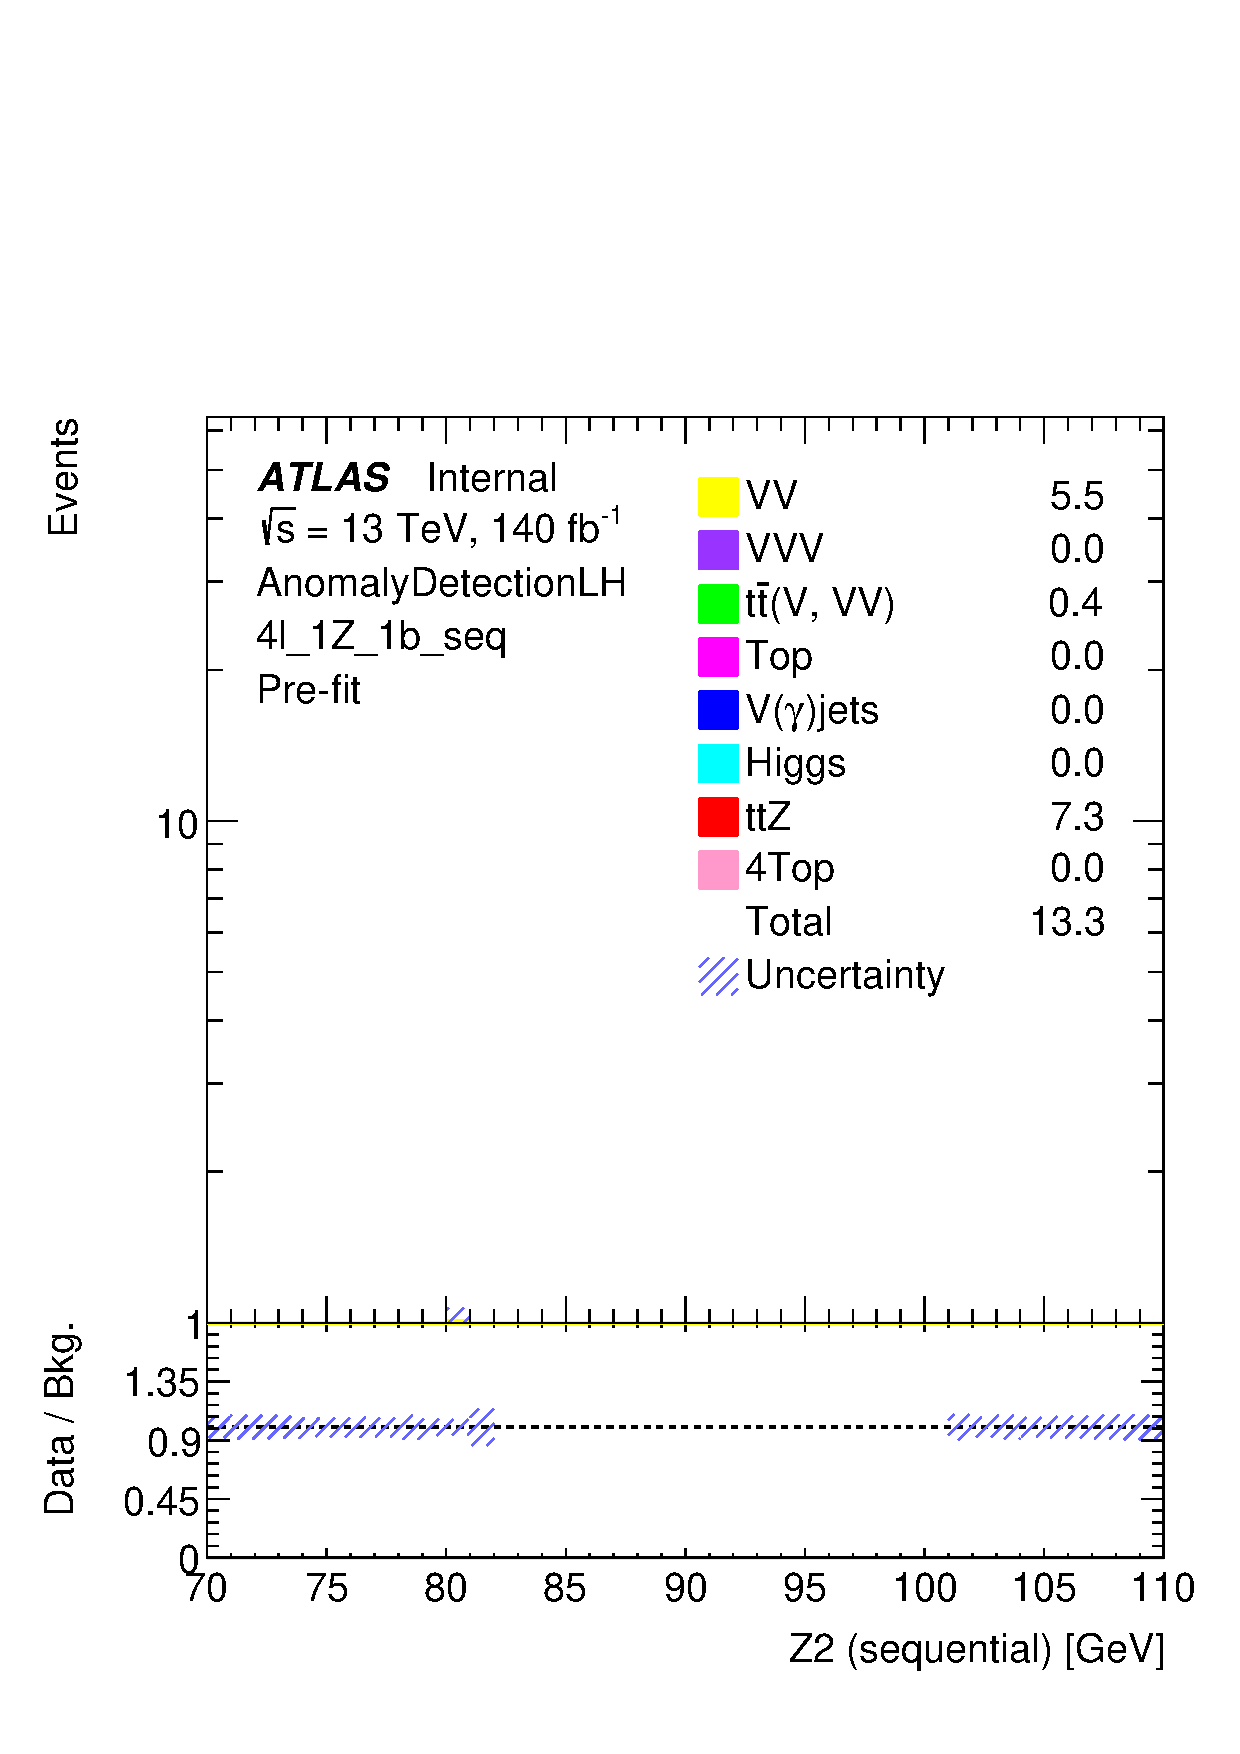
\includegraphics[width=0.24\textwidth]{plots/fourlepLH_run2/Plots/reg_4l_1Z_1b_seq_Z2_mass_seq_1GeV.pdf}  &

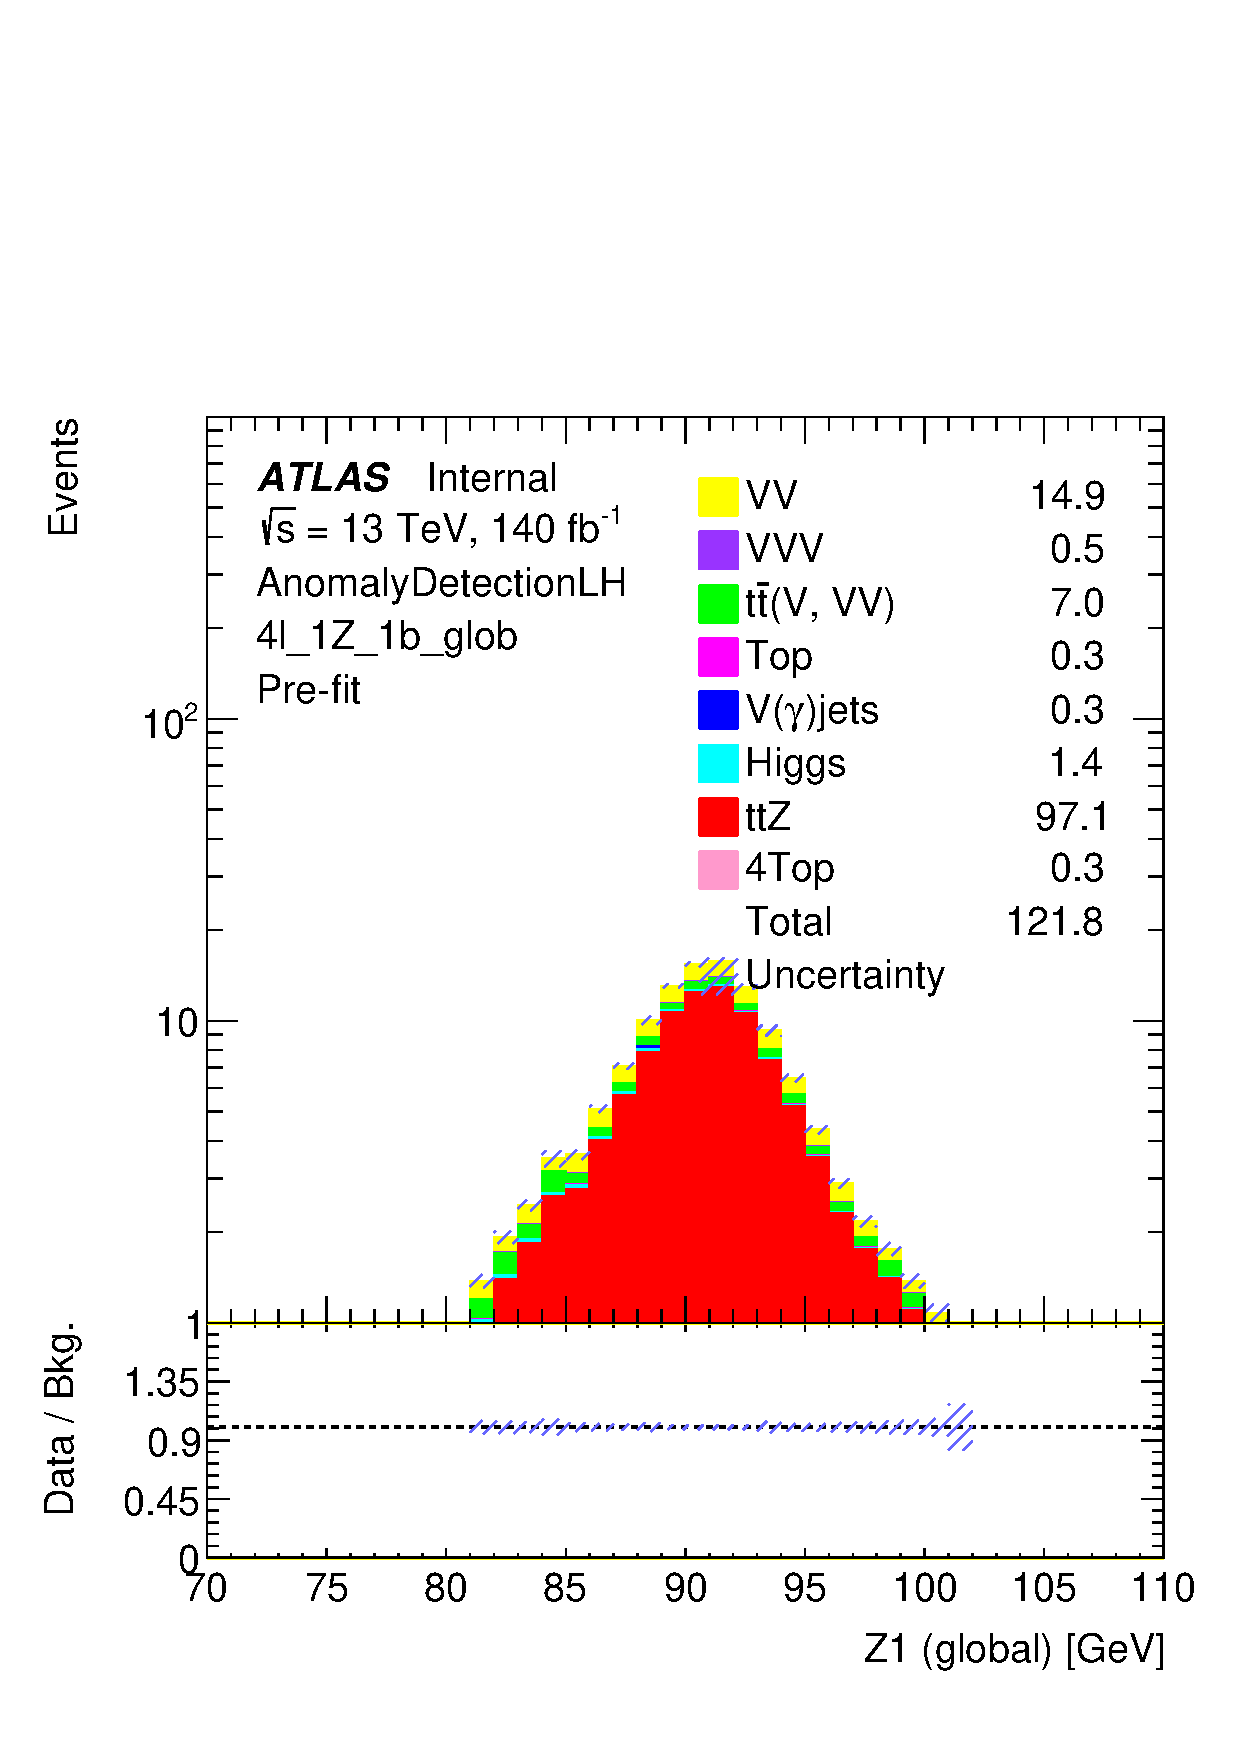
\includegraphics[width=0.24\textwidth]{plots/fourlepLH_run2/Plots/reg_4l_1Z_1b_glob_Z1_mass_glob_1GeV.pdf} &
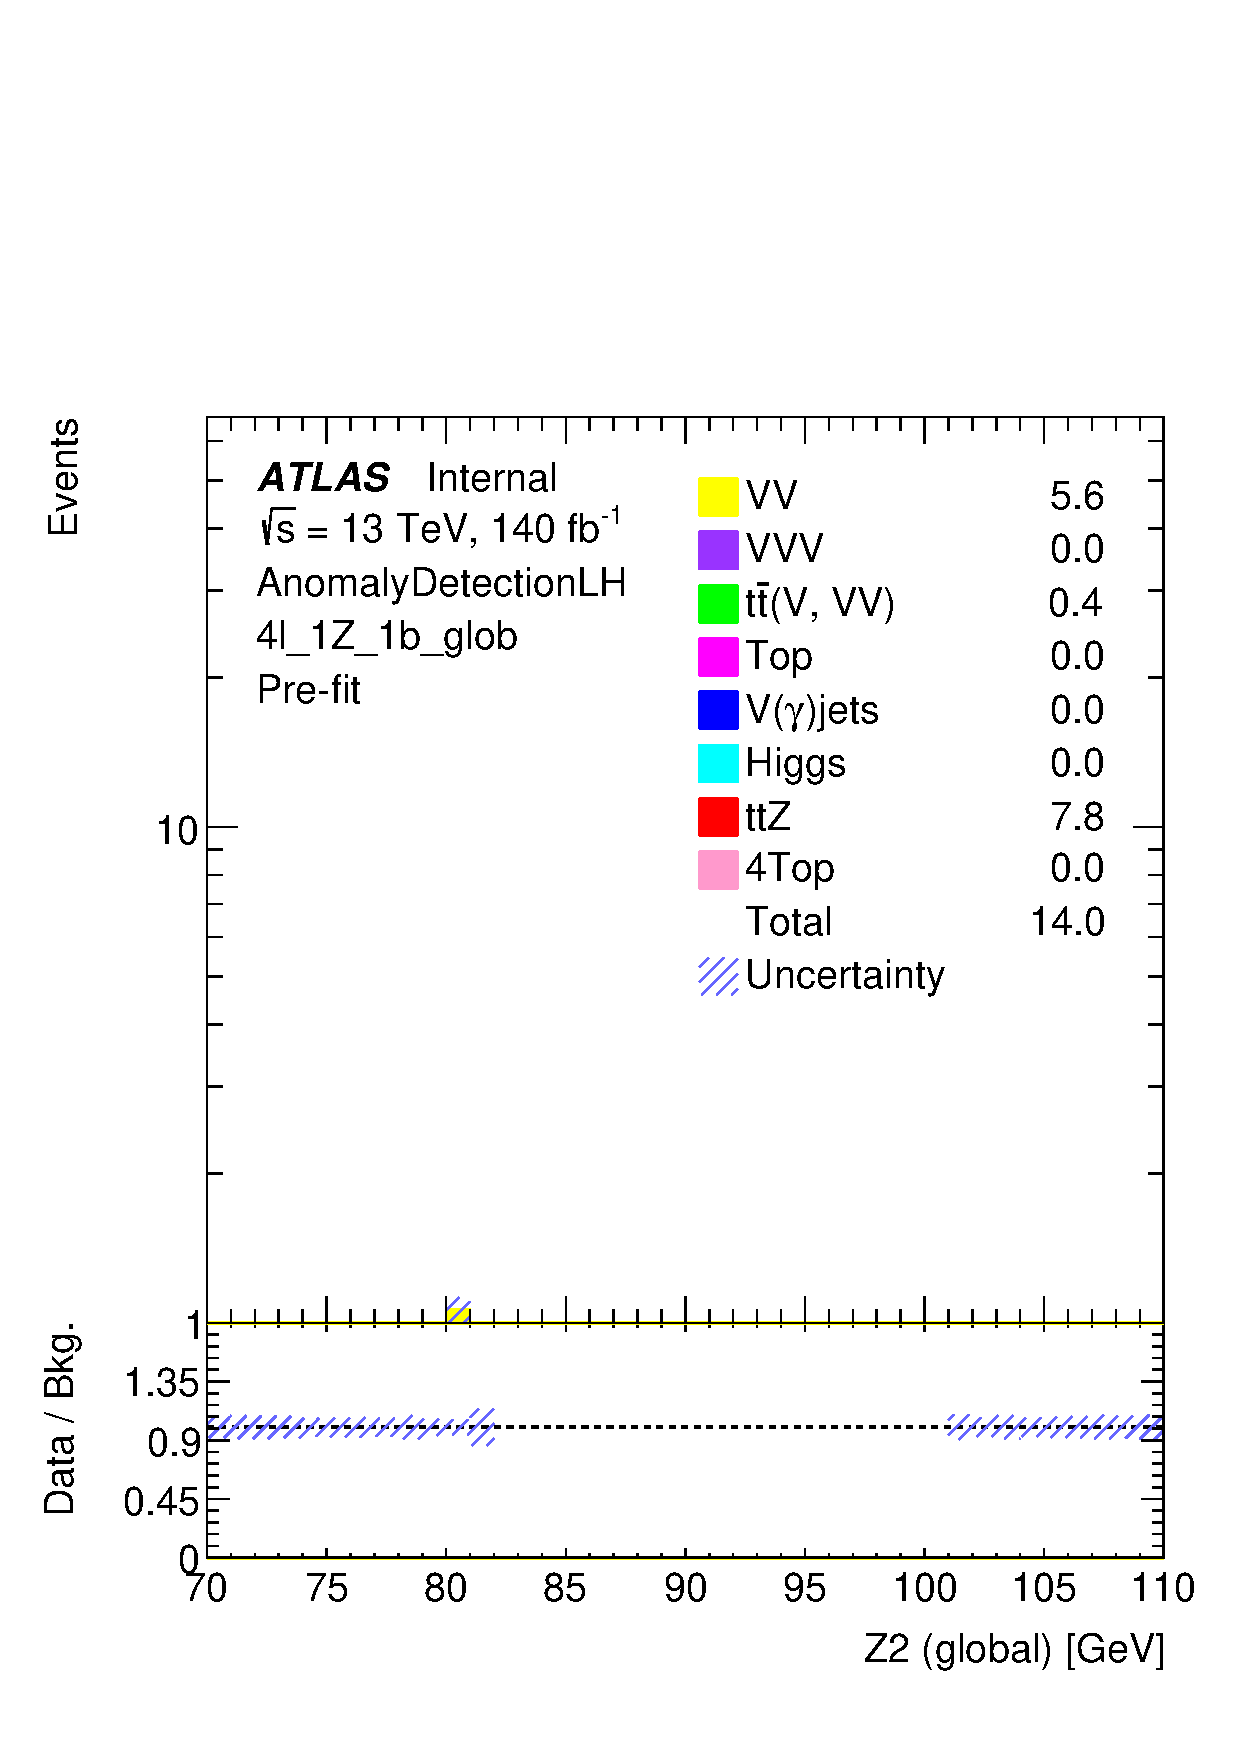
\includegraphics[width=0.24\textwidth]{plots/fourlepLH_run2/Plots/reg_4l_1Z_1b_glob_Z2_mass_glob_1GeV.pdf}\\

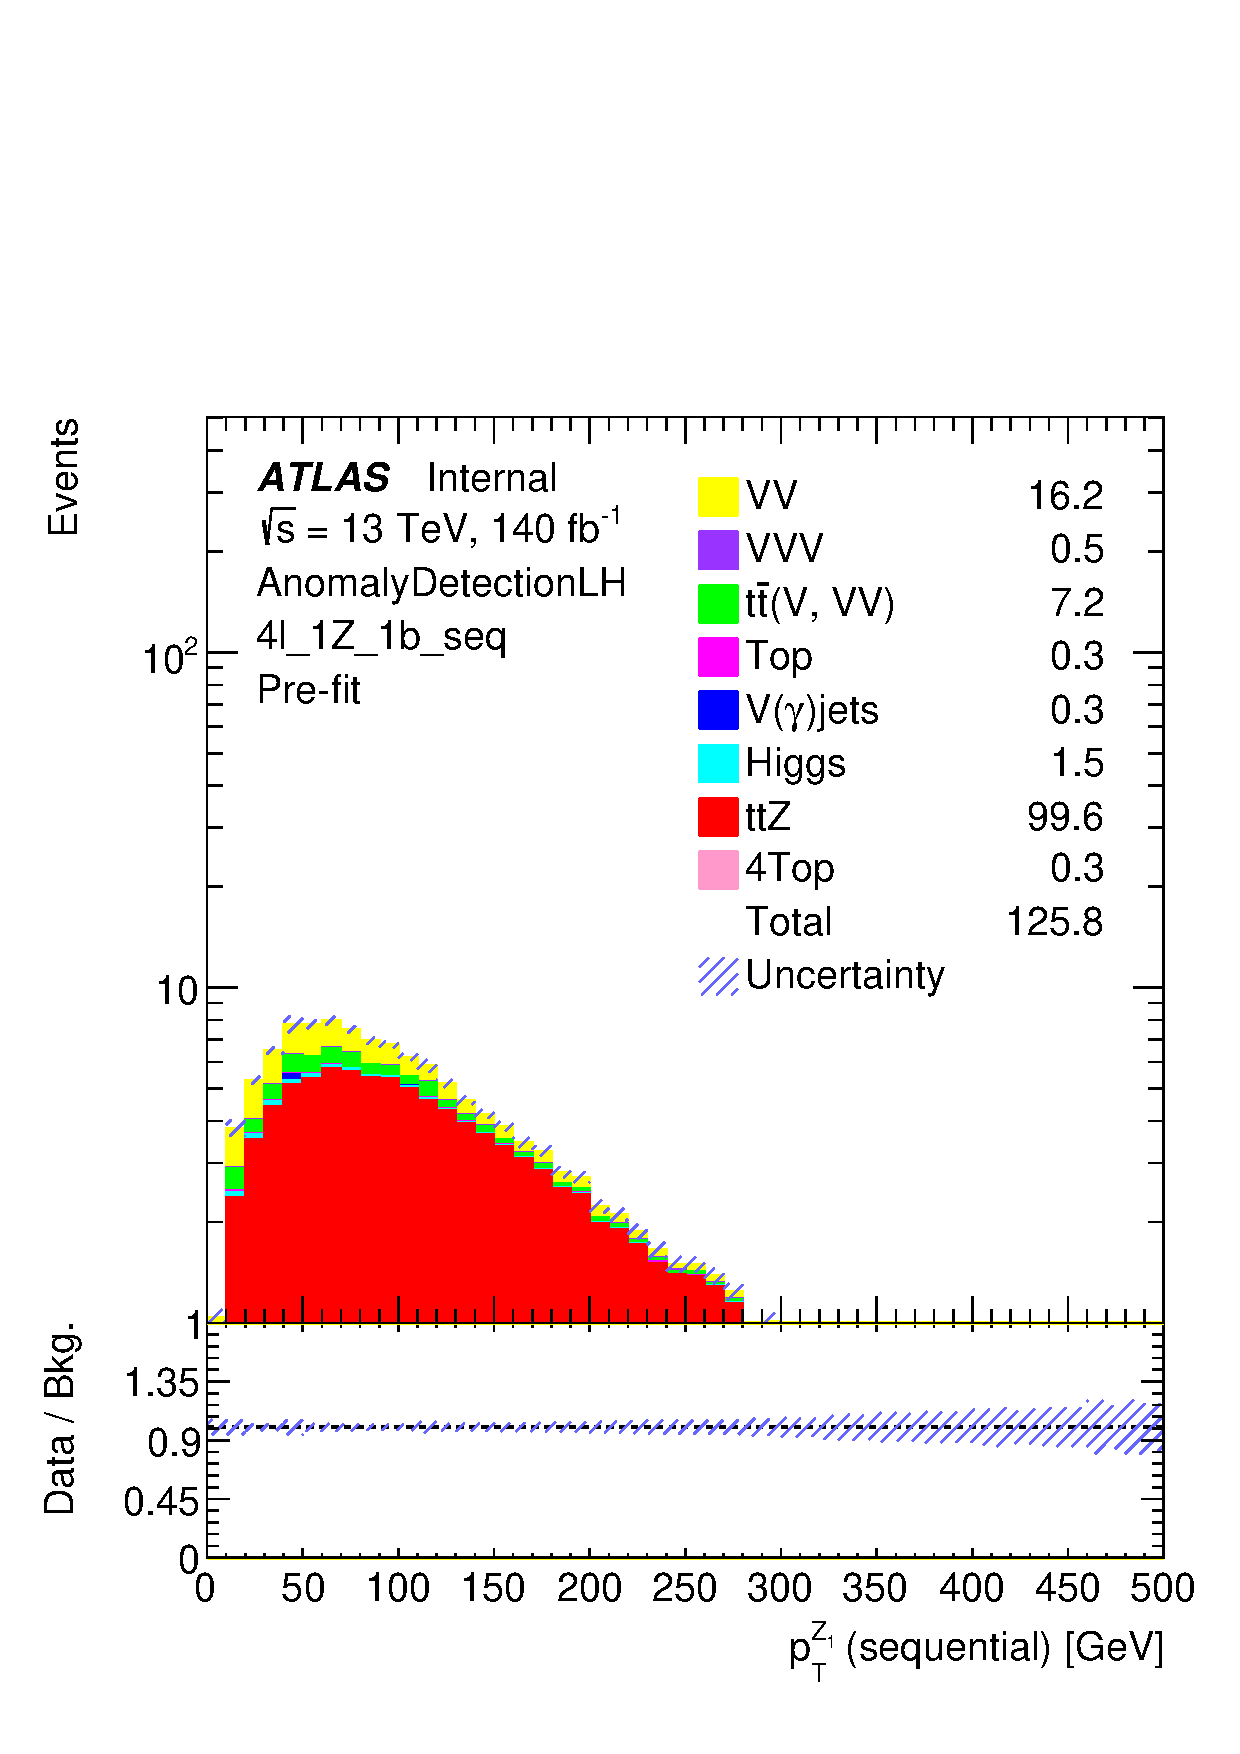
\includegraphics[width=0.24\textwidth]{plots/fourlepLH_run2/Plots/reg_4l_1Z_1b_seq_Z1_pt_seq.pdf} &
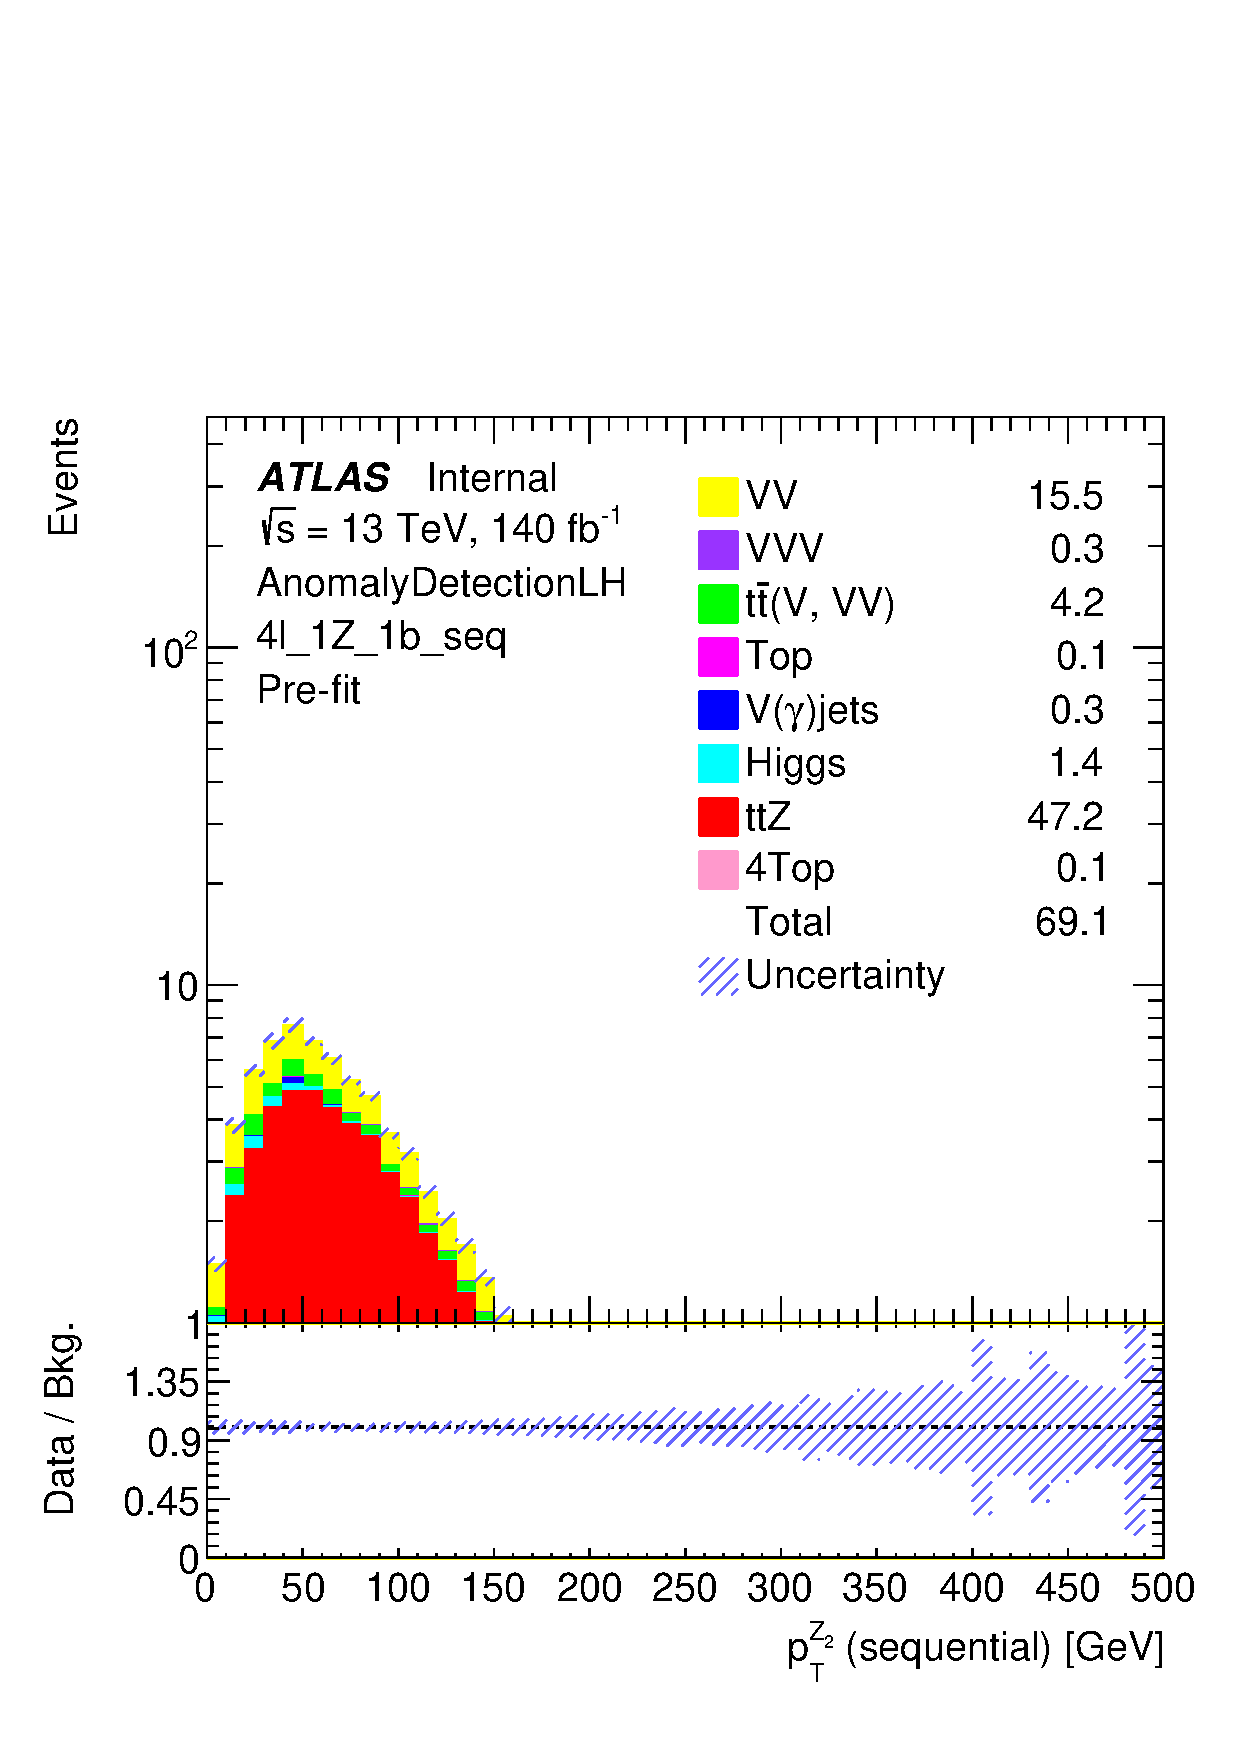
\includegraphics[width=0.24\textwidth]{plots/fourlepLH_run2/Plots/reg_4l_1Z_1b_seq_Z2_pt_seq.pdf}  &

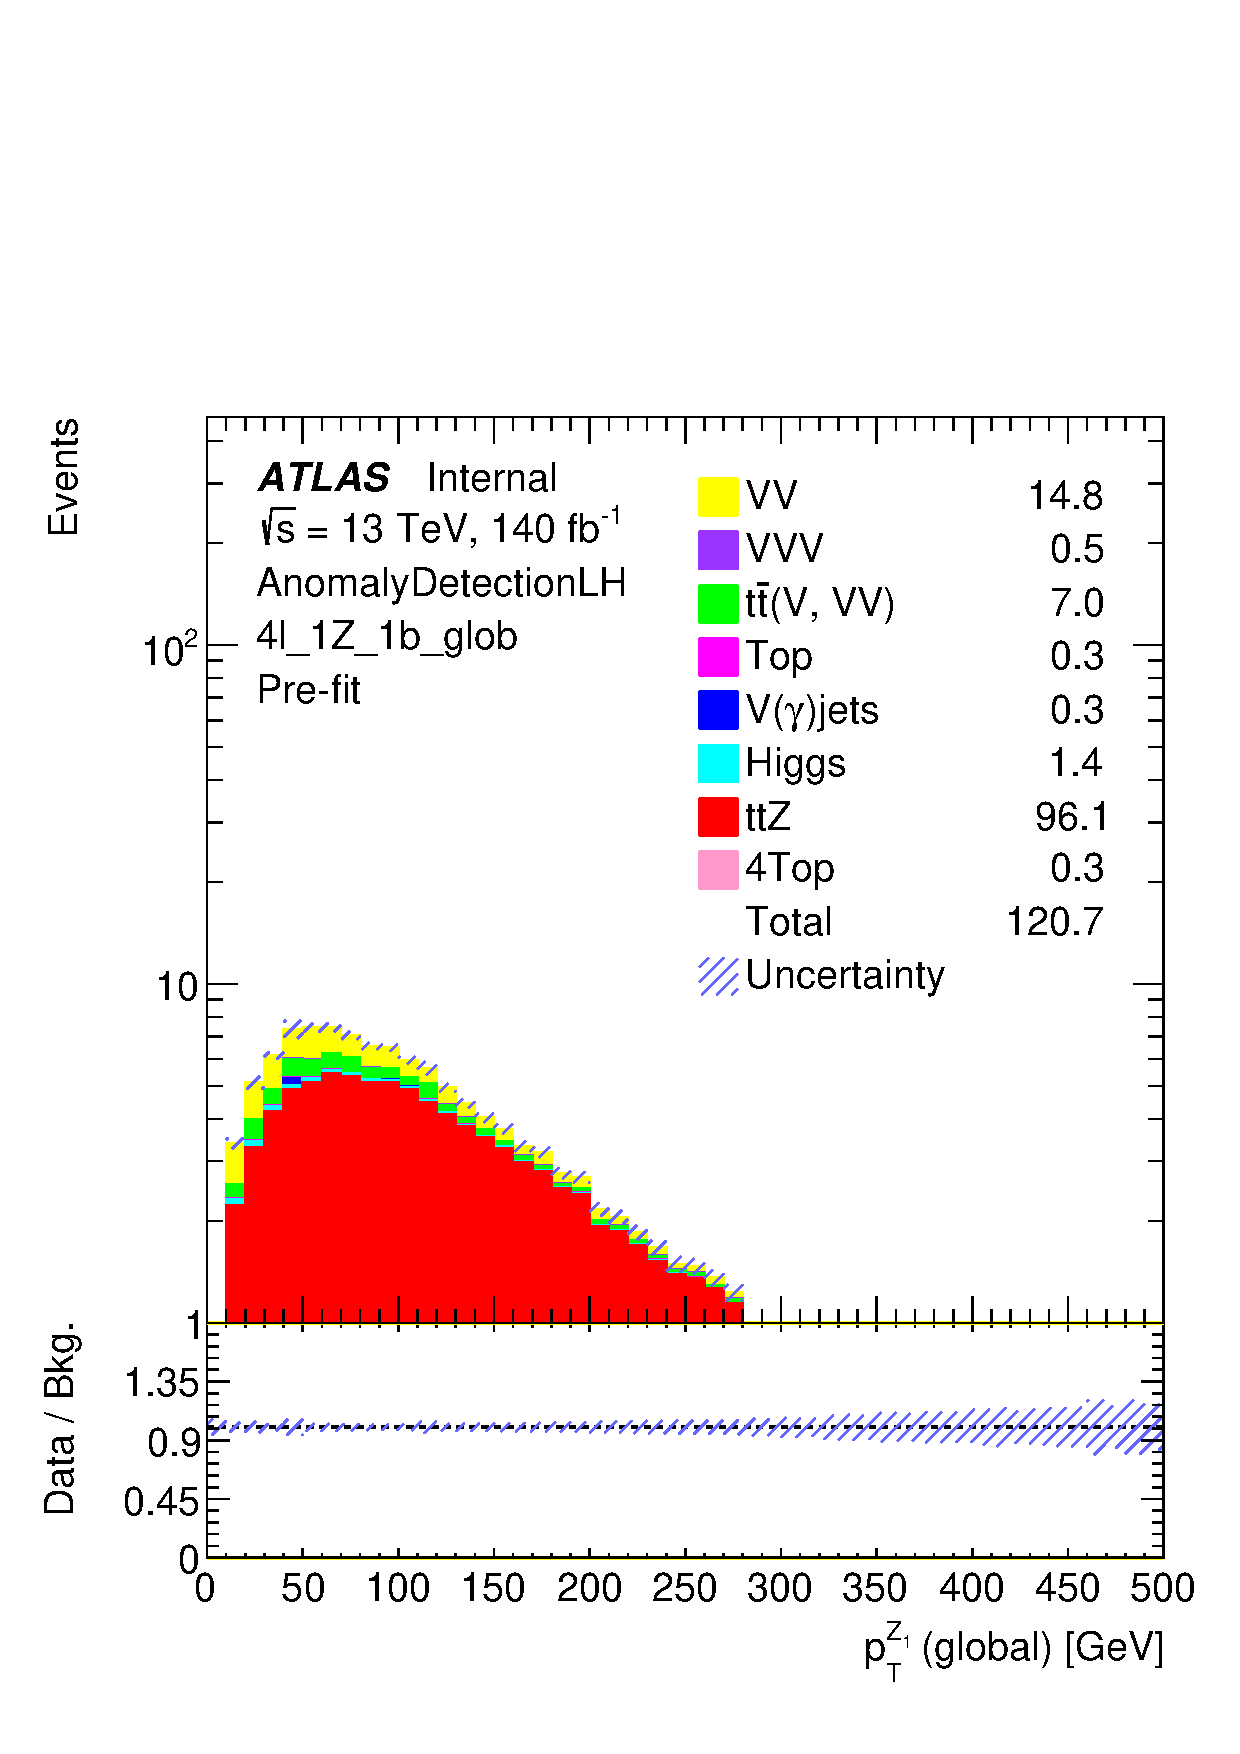
\includegraphics[width=0.24\textwidth]{plots/fourlepLH_run2/Plots/reg_4l_1Z_1b_glob_Z1_pt_glob.pdf} &
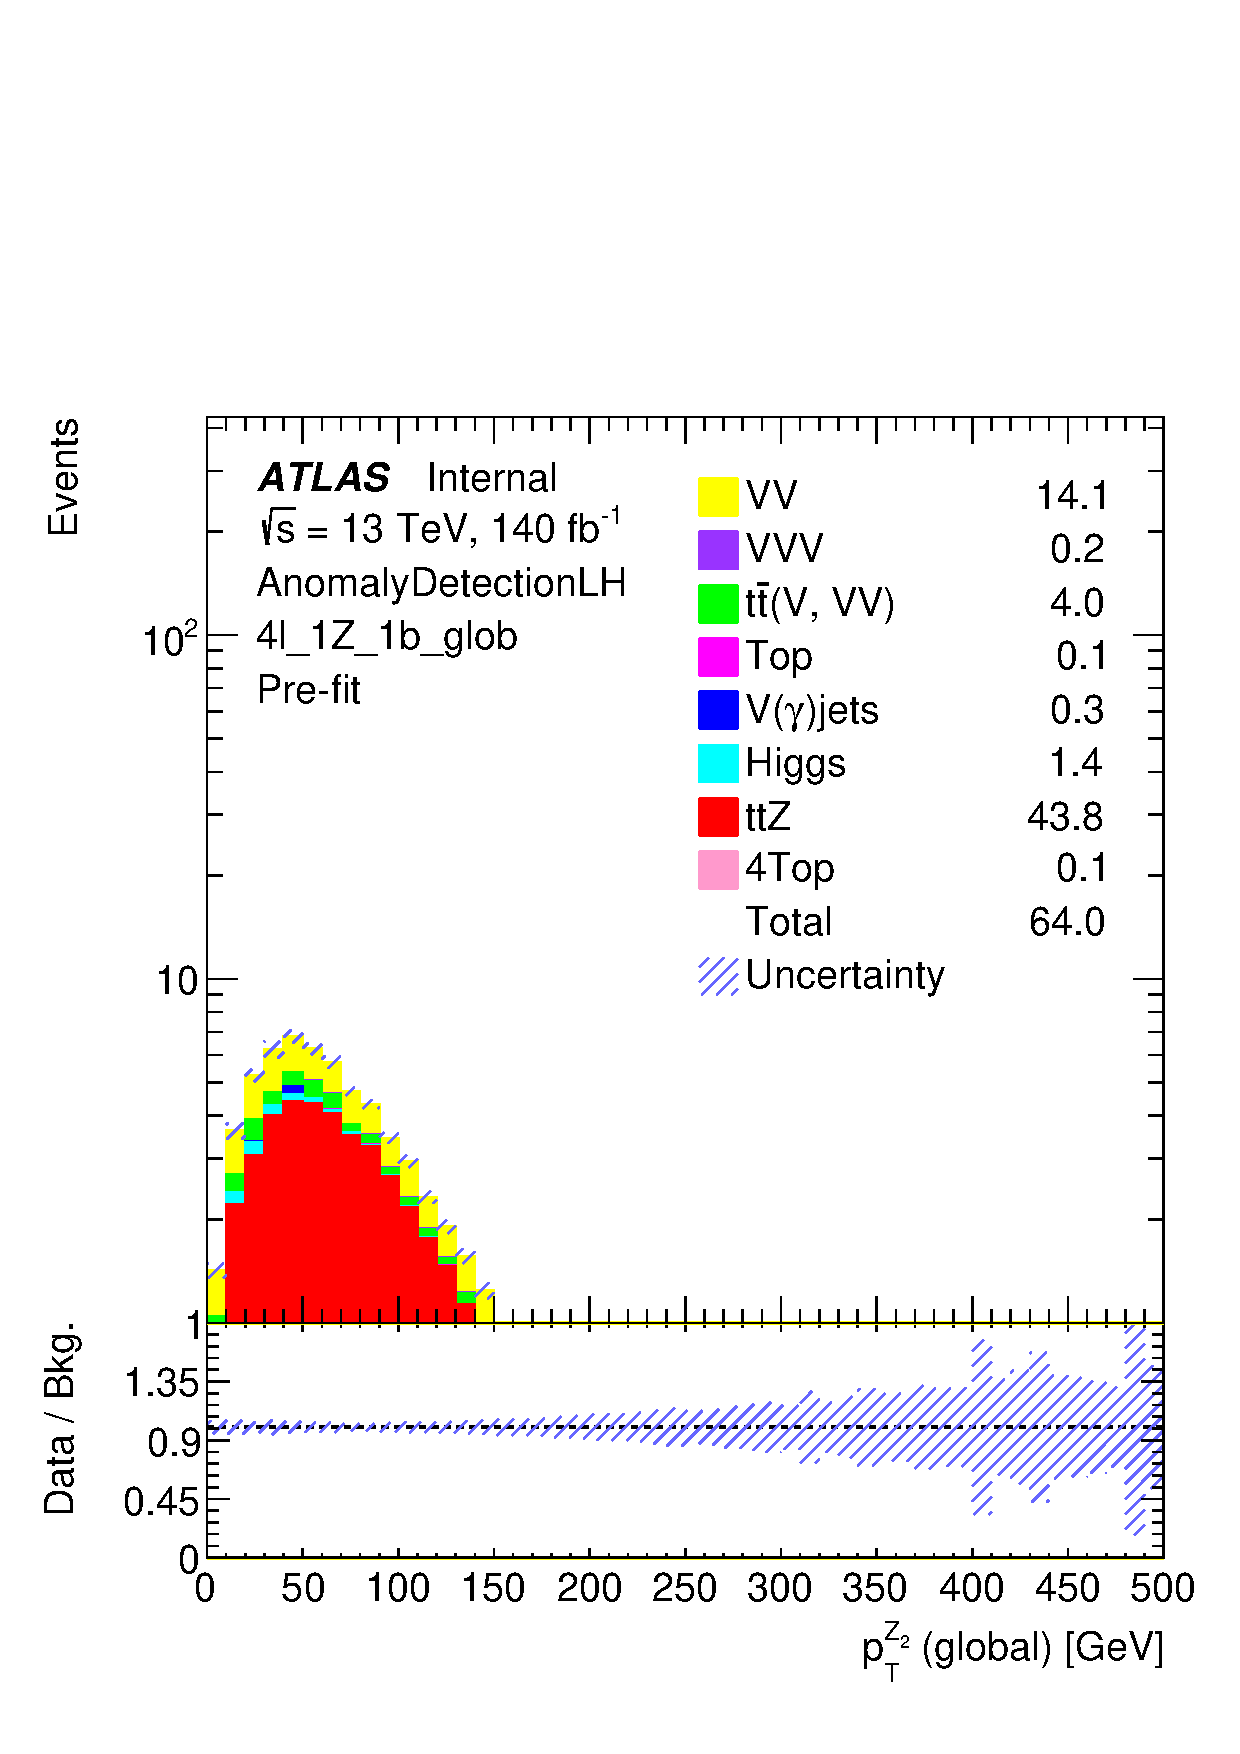
\includegraphics[width=0.24\textwidth]{plots/fourlepLH_run2/Plots/reg_4l_1Z_1b_glob_Z2_pt_glob.pdf}
\end{tabular}
\end{frame}

\begin{frame}{\texttt{Results: 4l\_1Z\_1b}}
\begin{tabular}{cccccc}
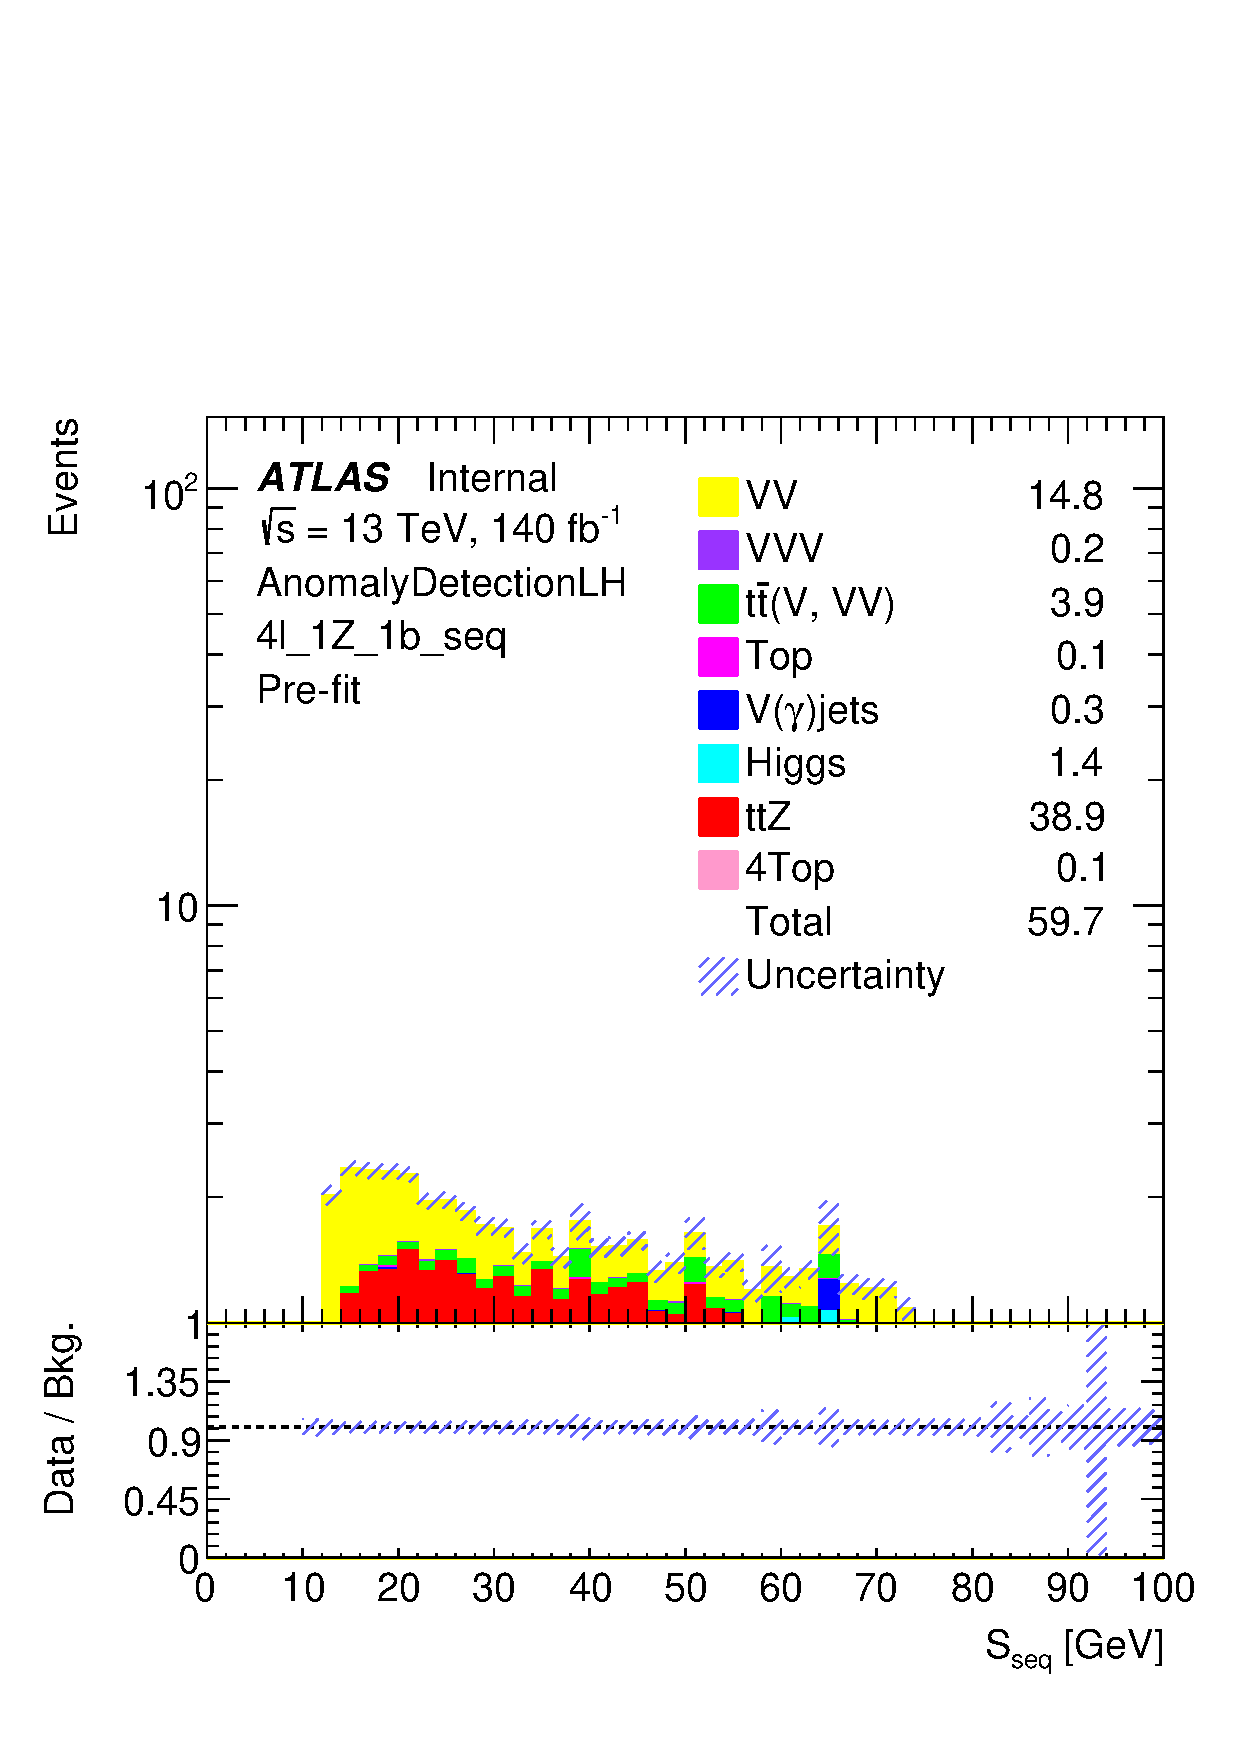
\includegraphics[width=0.24\textwidth]{plots/fourlepLH_run2/Plots/reg_4l_1Z_1b_seq_Zscore_seq.pdf} & 
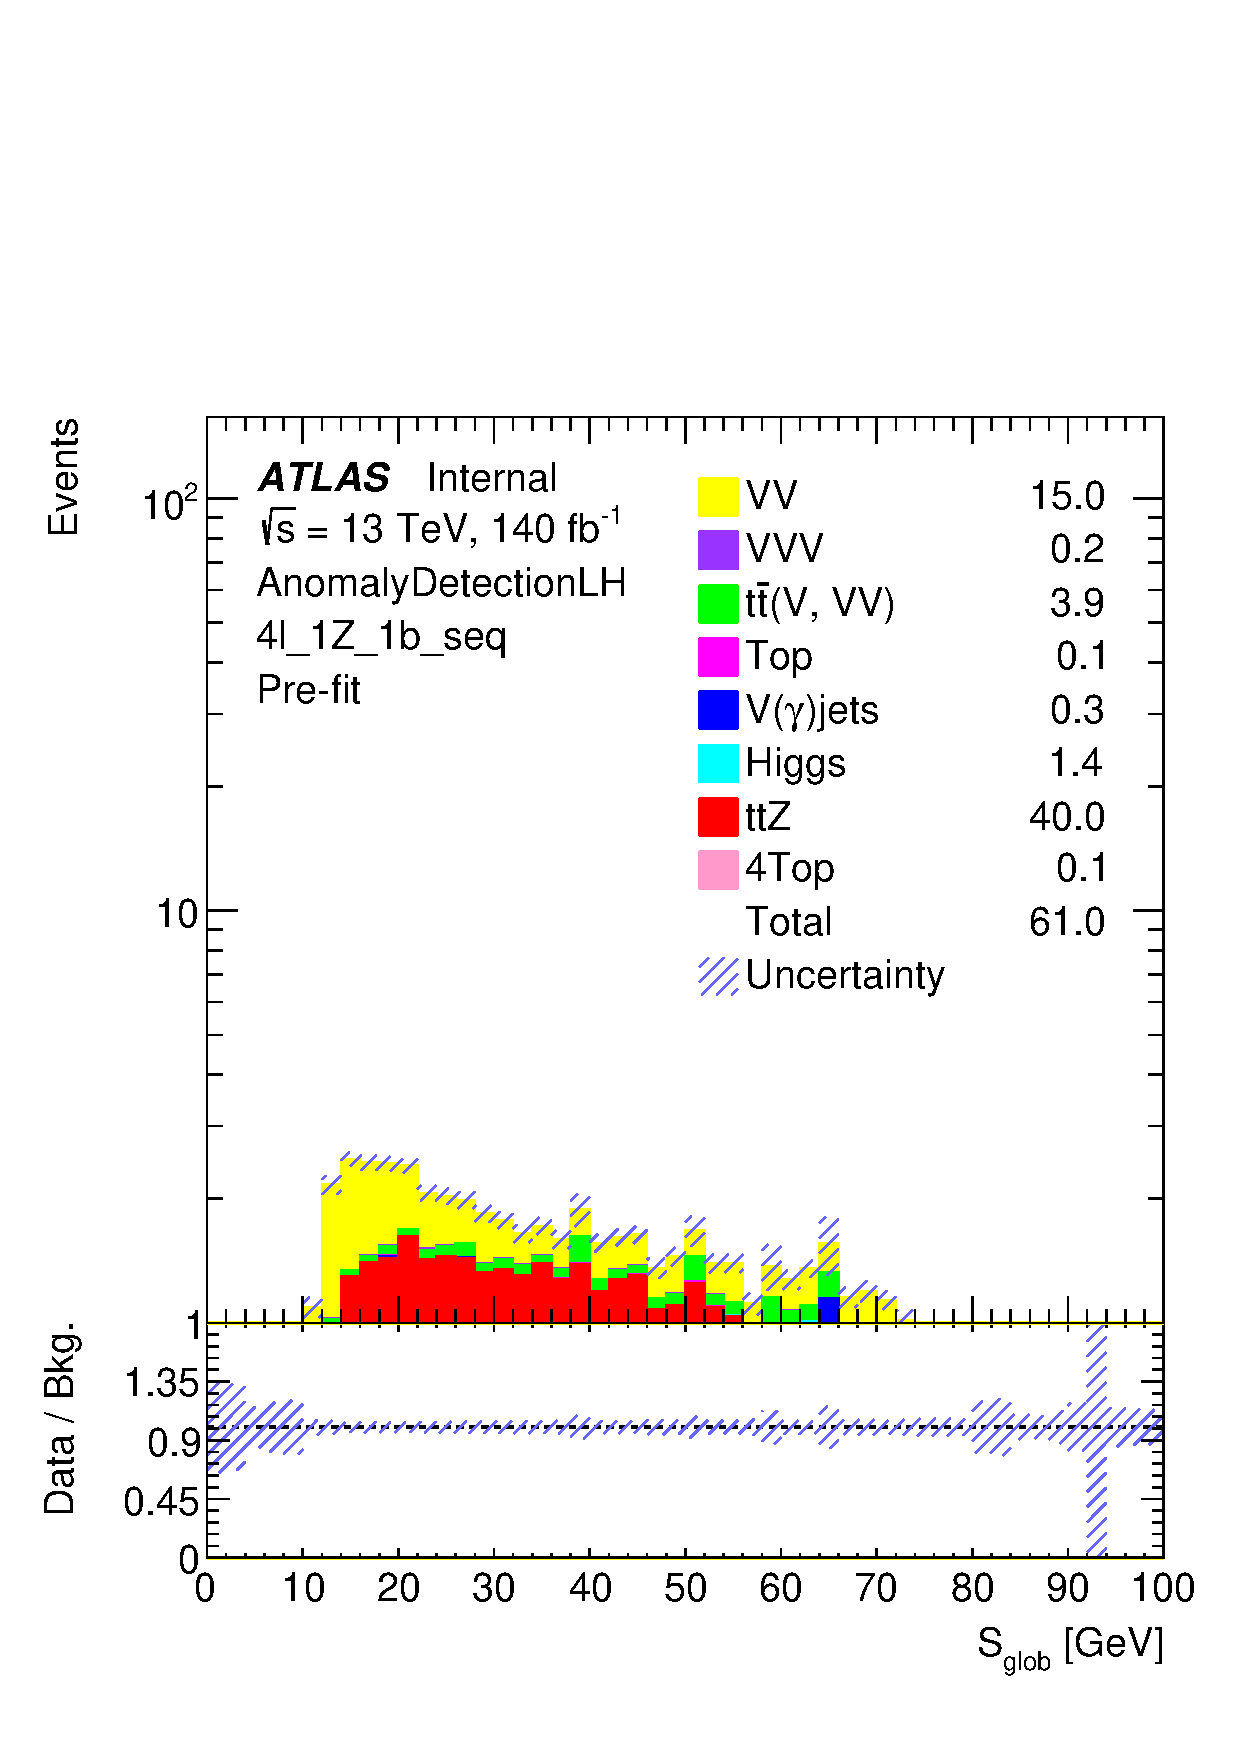
\includegraphics[width=0.24\textwidth]{plots/fourlepLH_run2/Plots/reg_4l_1Z_1b_seq_Zscore_glob.pdf}&
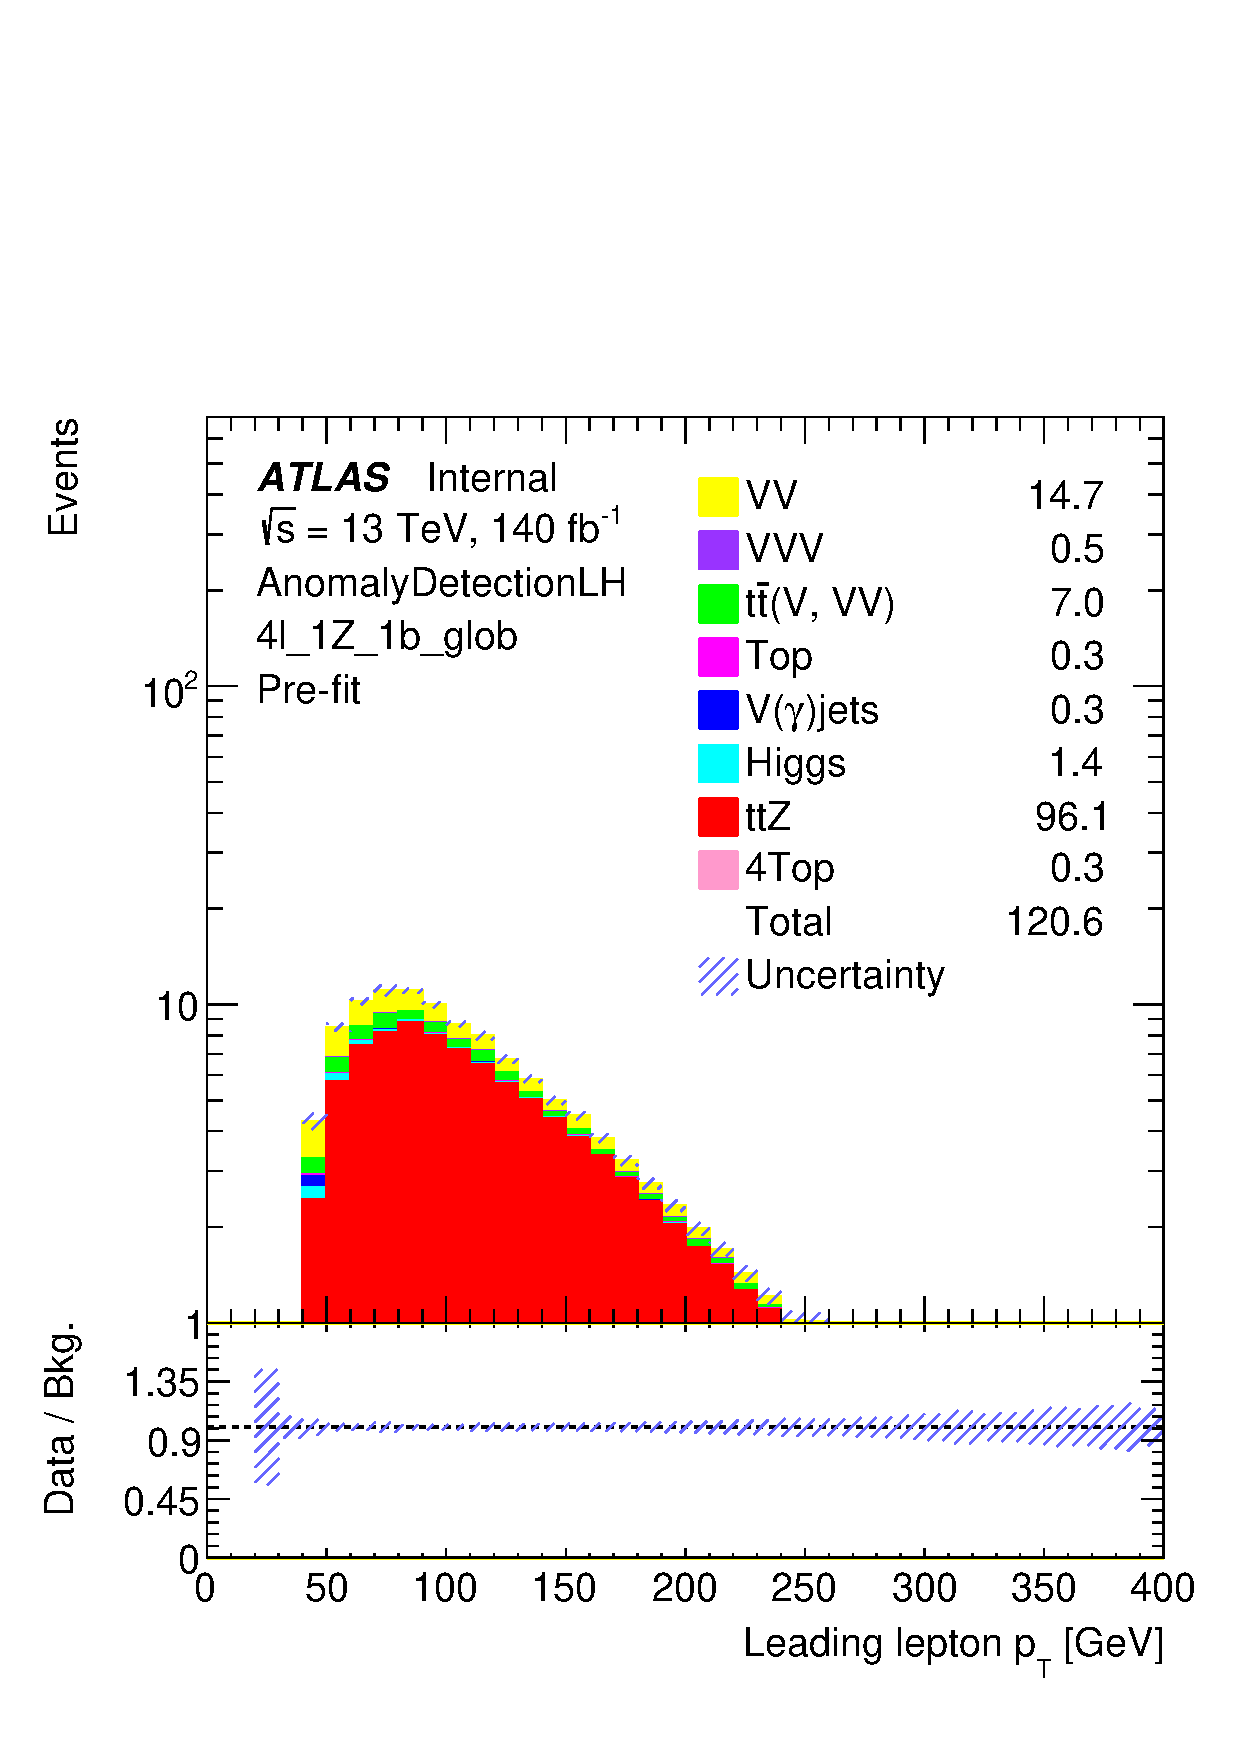
\includegraphics[width=0.24\textwidth]{plots/fourlepLH_run2/Plots/reg_4l_1Z_1b_seq_deltaZscore.pdf}\\

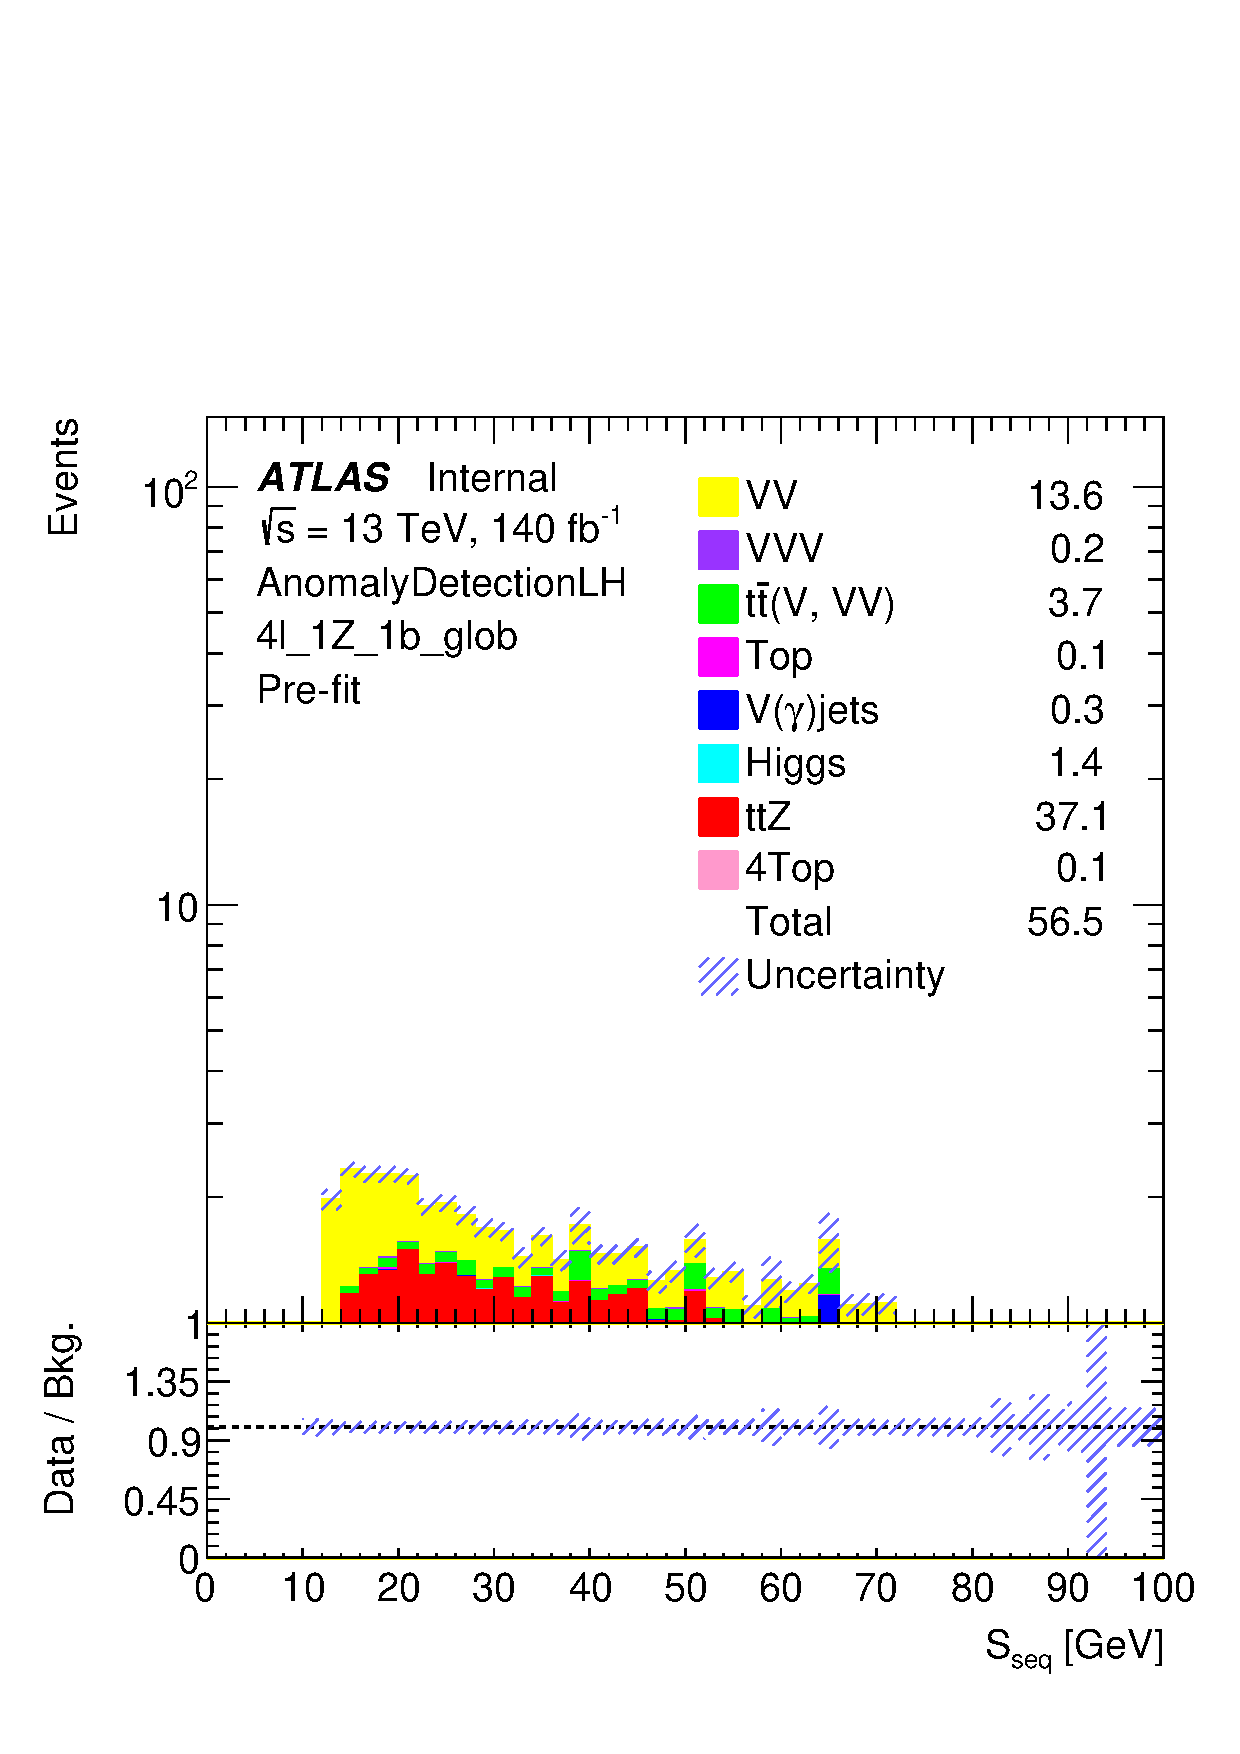
\includegraphics[width=0.24\textwidth]{plots/fourlepLH_run2/Plots/reg_4l_1Z_1b_glob_Zscore_seq.pdf} & 
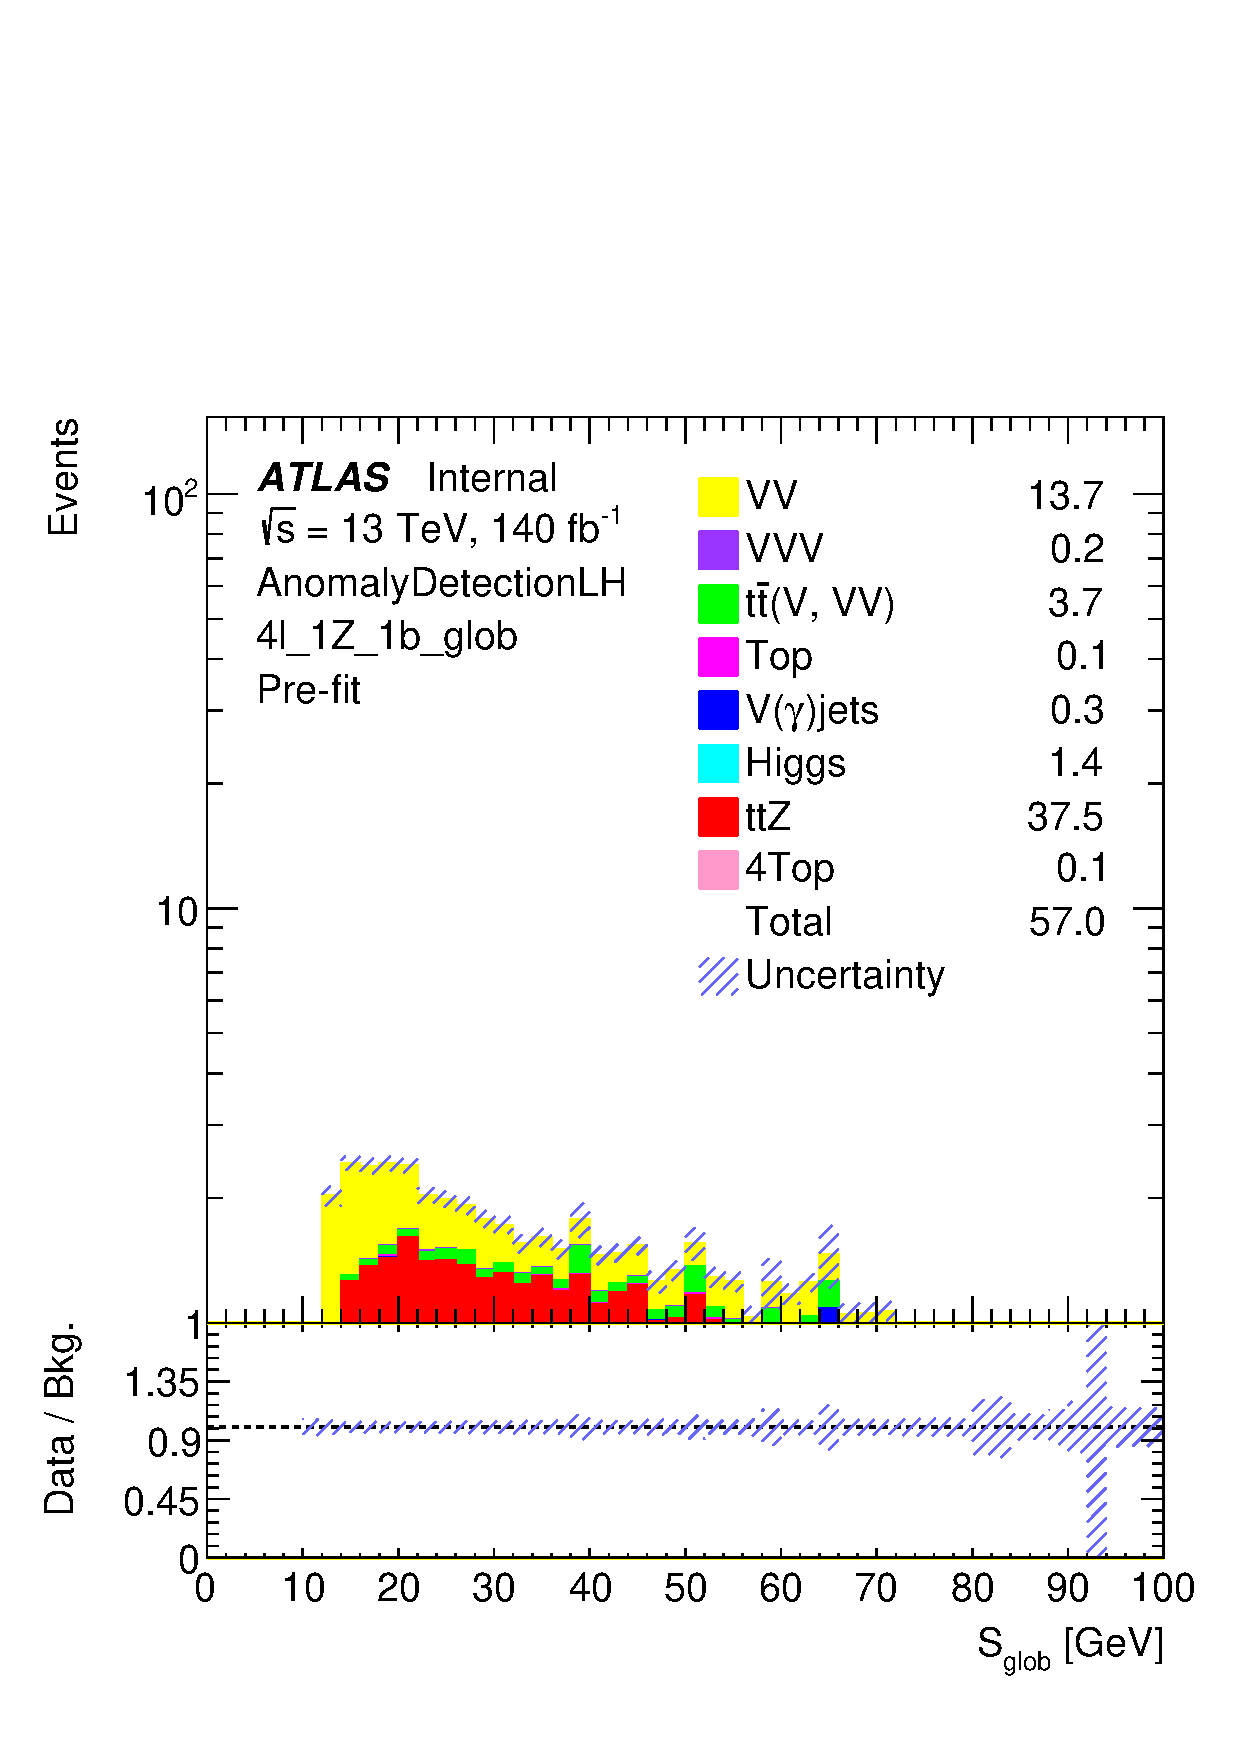
\includegraphics[width=0.24\textwidth]{plots/fourlepLH_run2/Plots/reg_4l_1Z_1b_glob_Zscore_glob.pdf}&
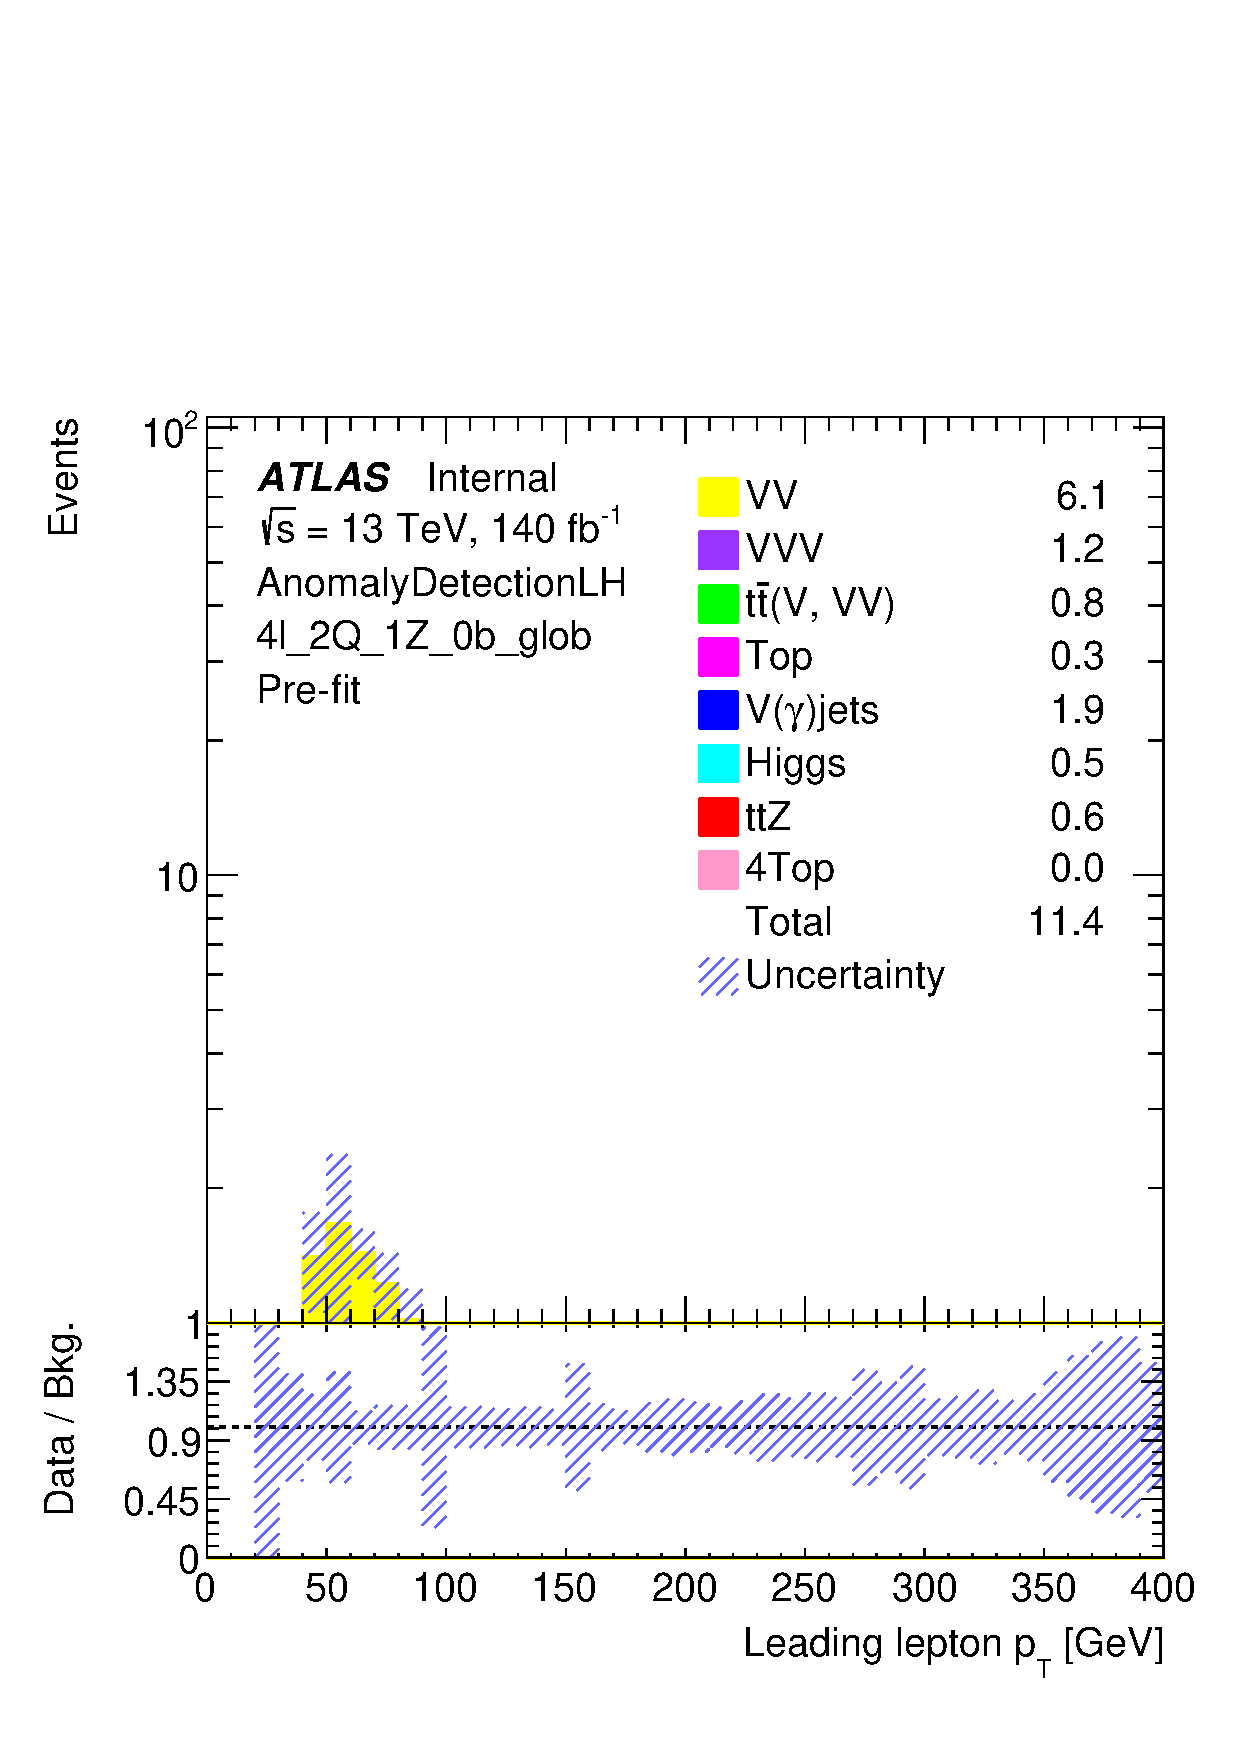
\includegraphics[width=0.24\textwidth]{plots/fourlepLH_run2/Plots/reg_4l_1Z_1b_glob_deltaZscore.pdf}
\end{tabular}
\end{frame}


\begin{frame}{\texttt{Results: 4l\_1Z\_1b}}
\begin{tabular}{cccccc}

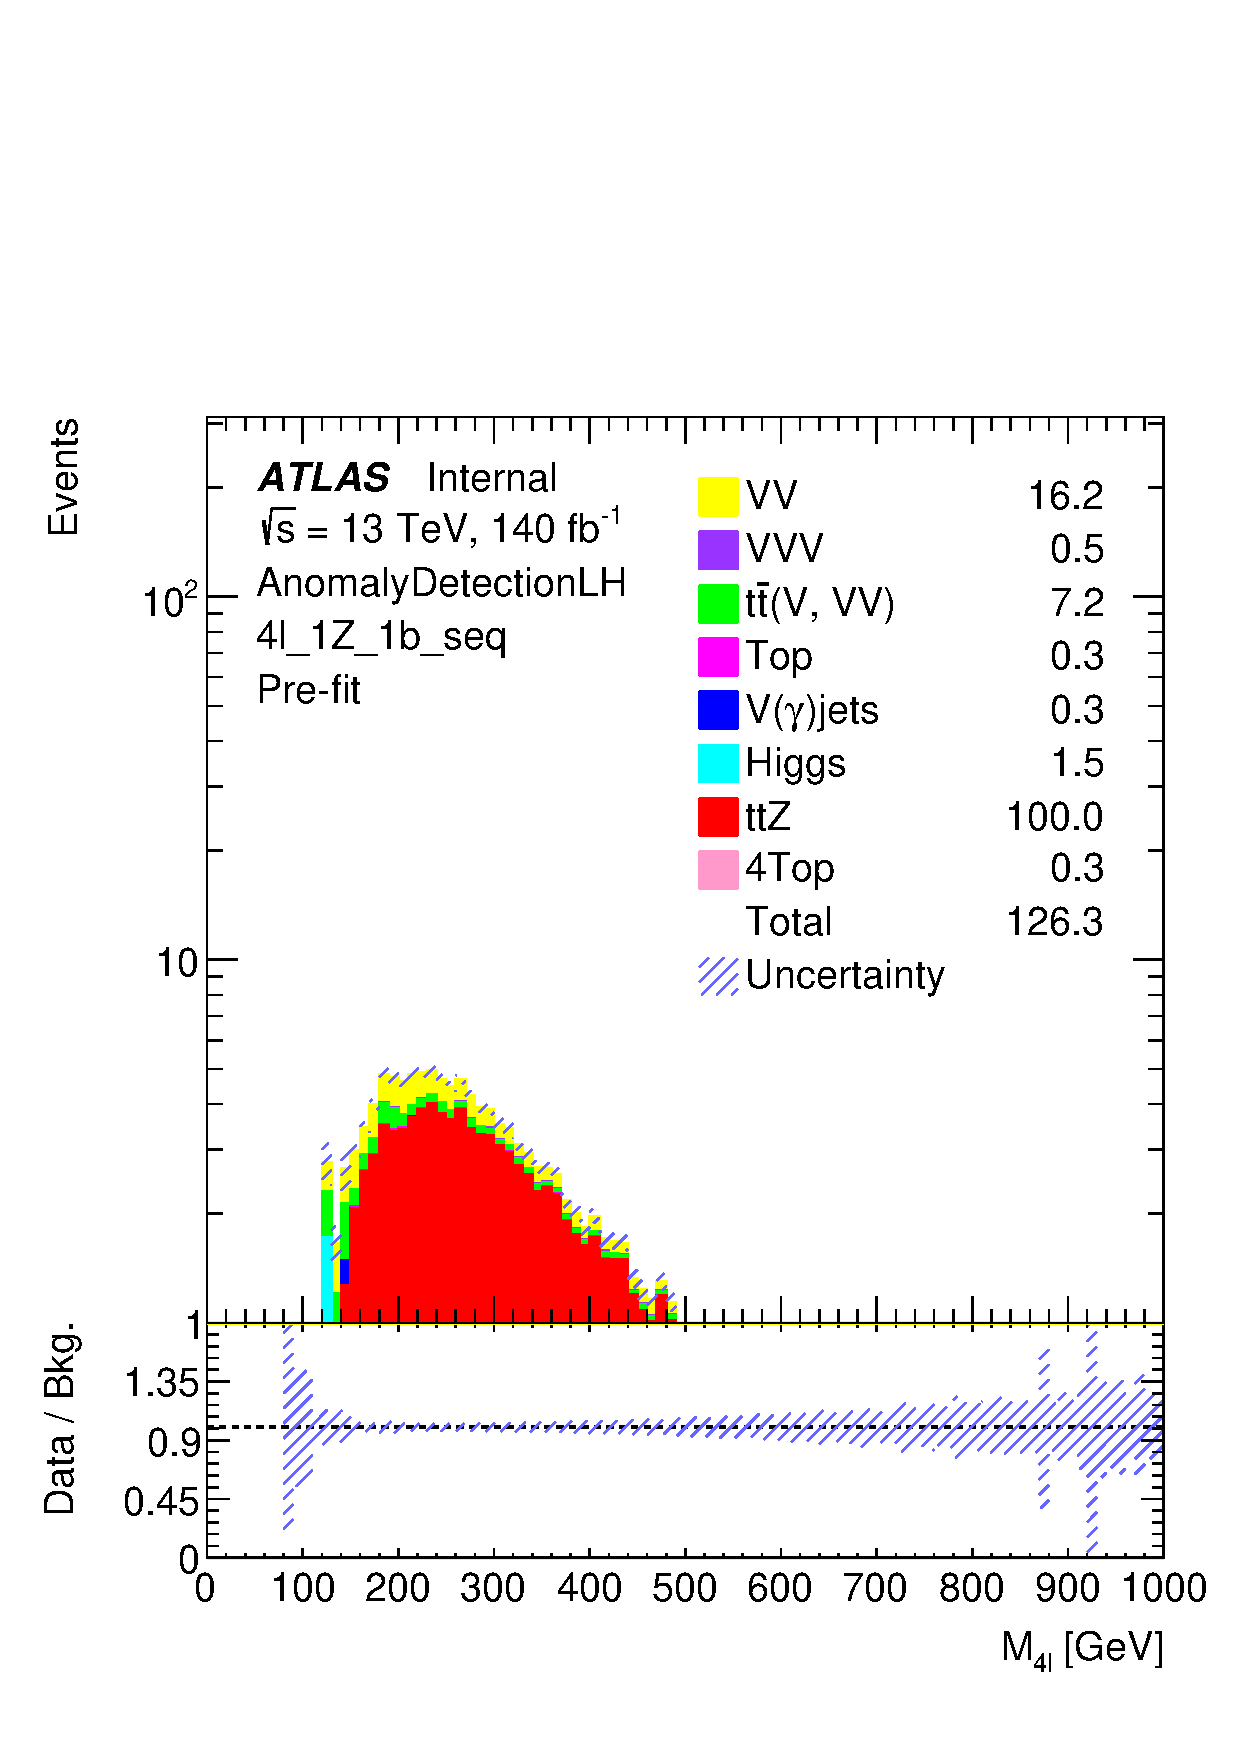
\includegraphics[width=0.24\textwidth]{plots/fourlepLH_run2/Plots/reg_4l_1Z_1b_seq_m4l.pdf} &
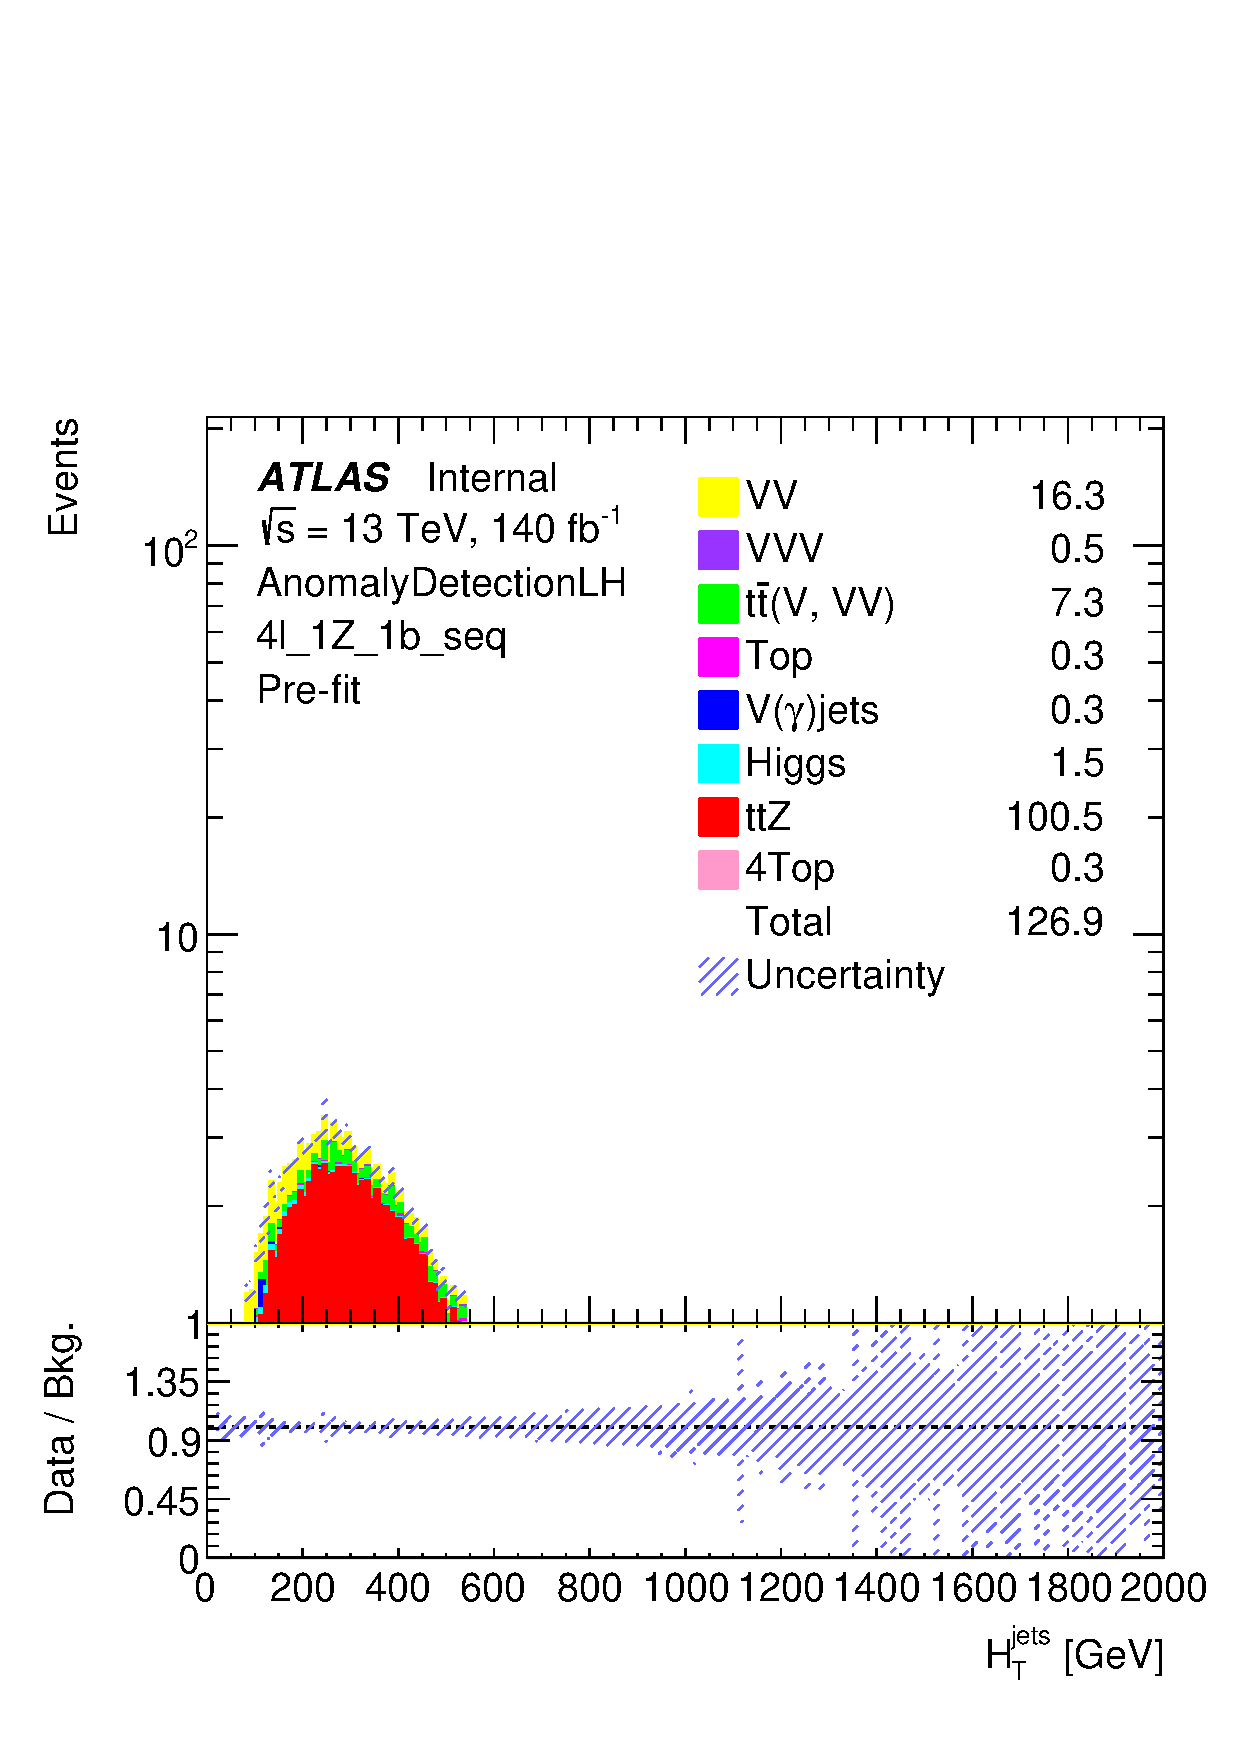
\includegraphics[width=0.24\textwidth]{plots/fourlepLH_run2/Plots/reg_4l_1Z_1b_seq_HT_jets.pdf} &
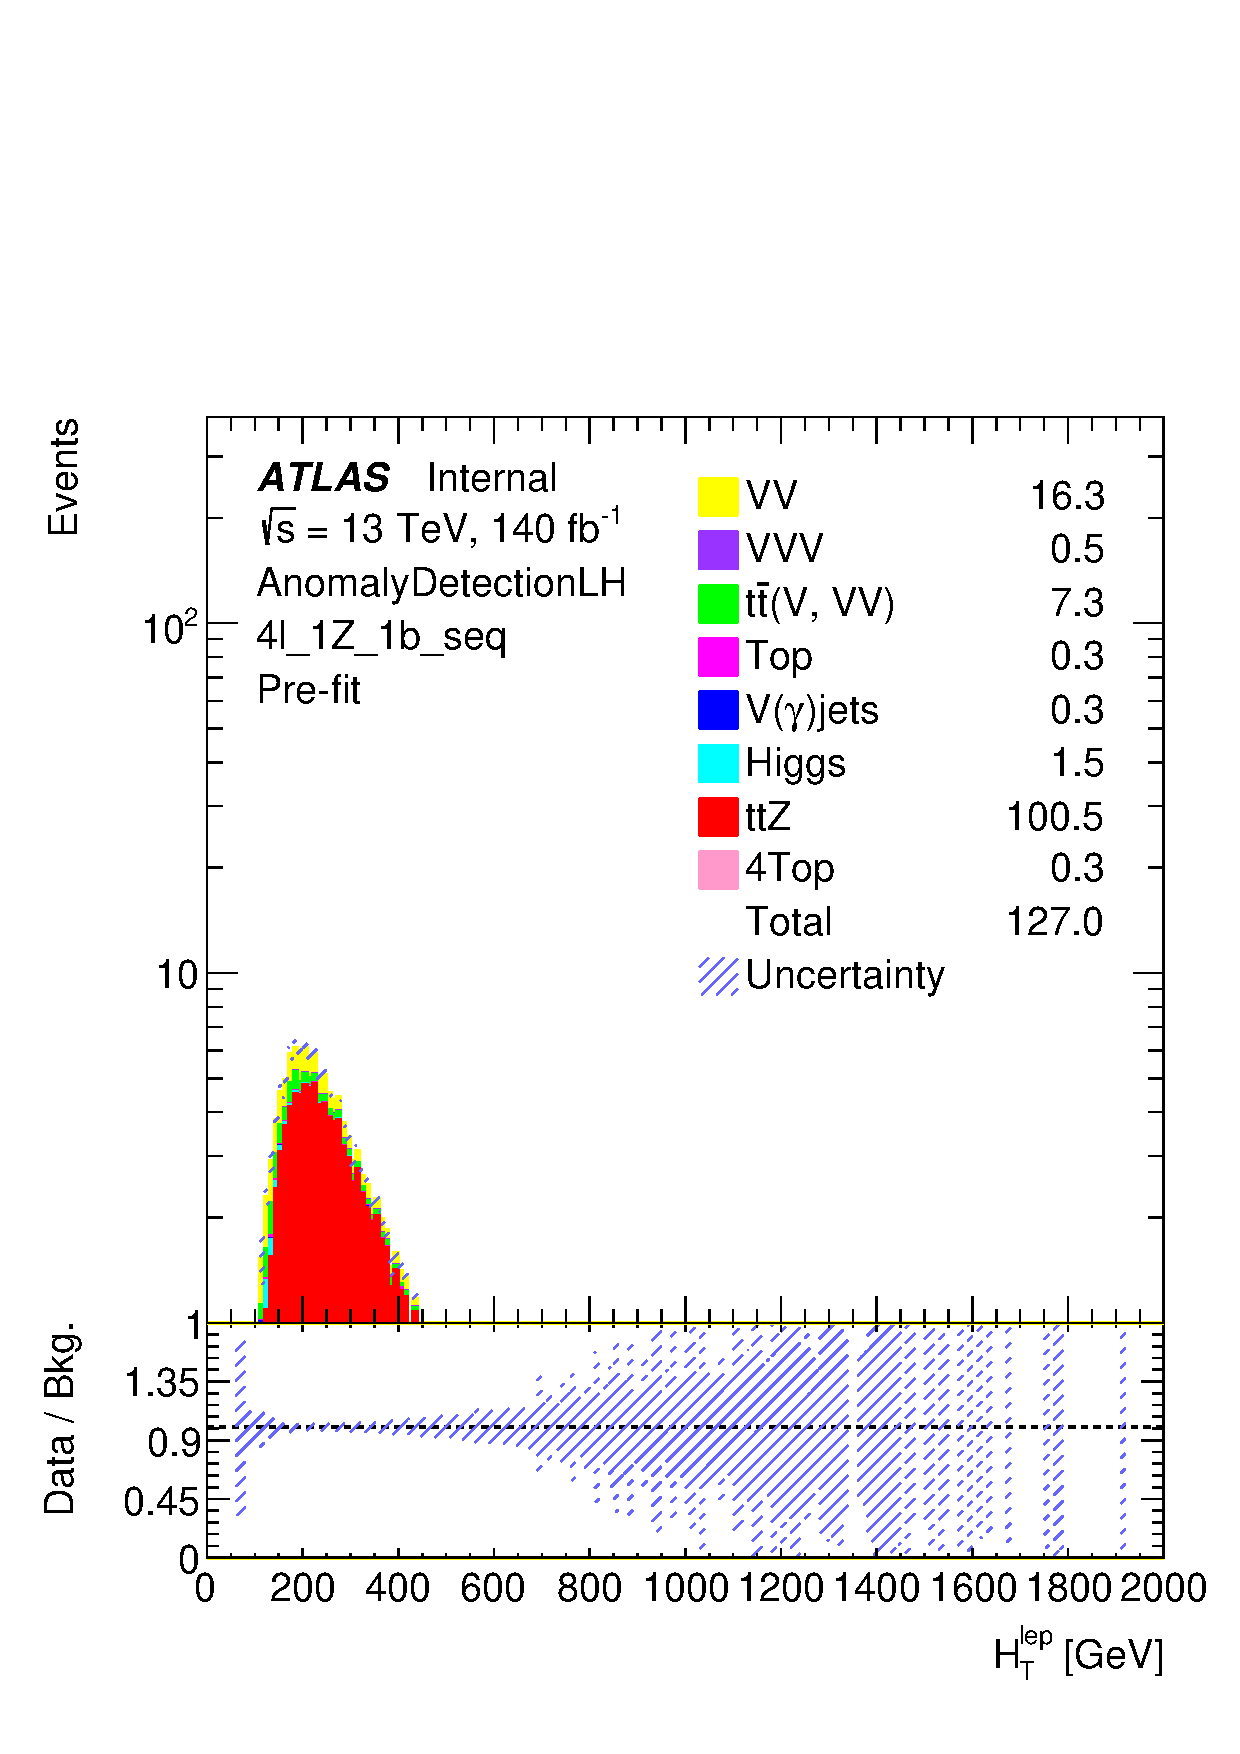
\includegraphics[width=0.24\textwidth]{plots/fourlepLH_run2/Plots/reg_4l_1Z_1b_seq_HT_lep.pdf} &
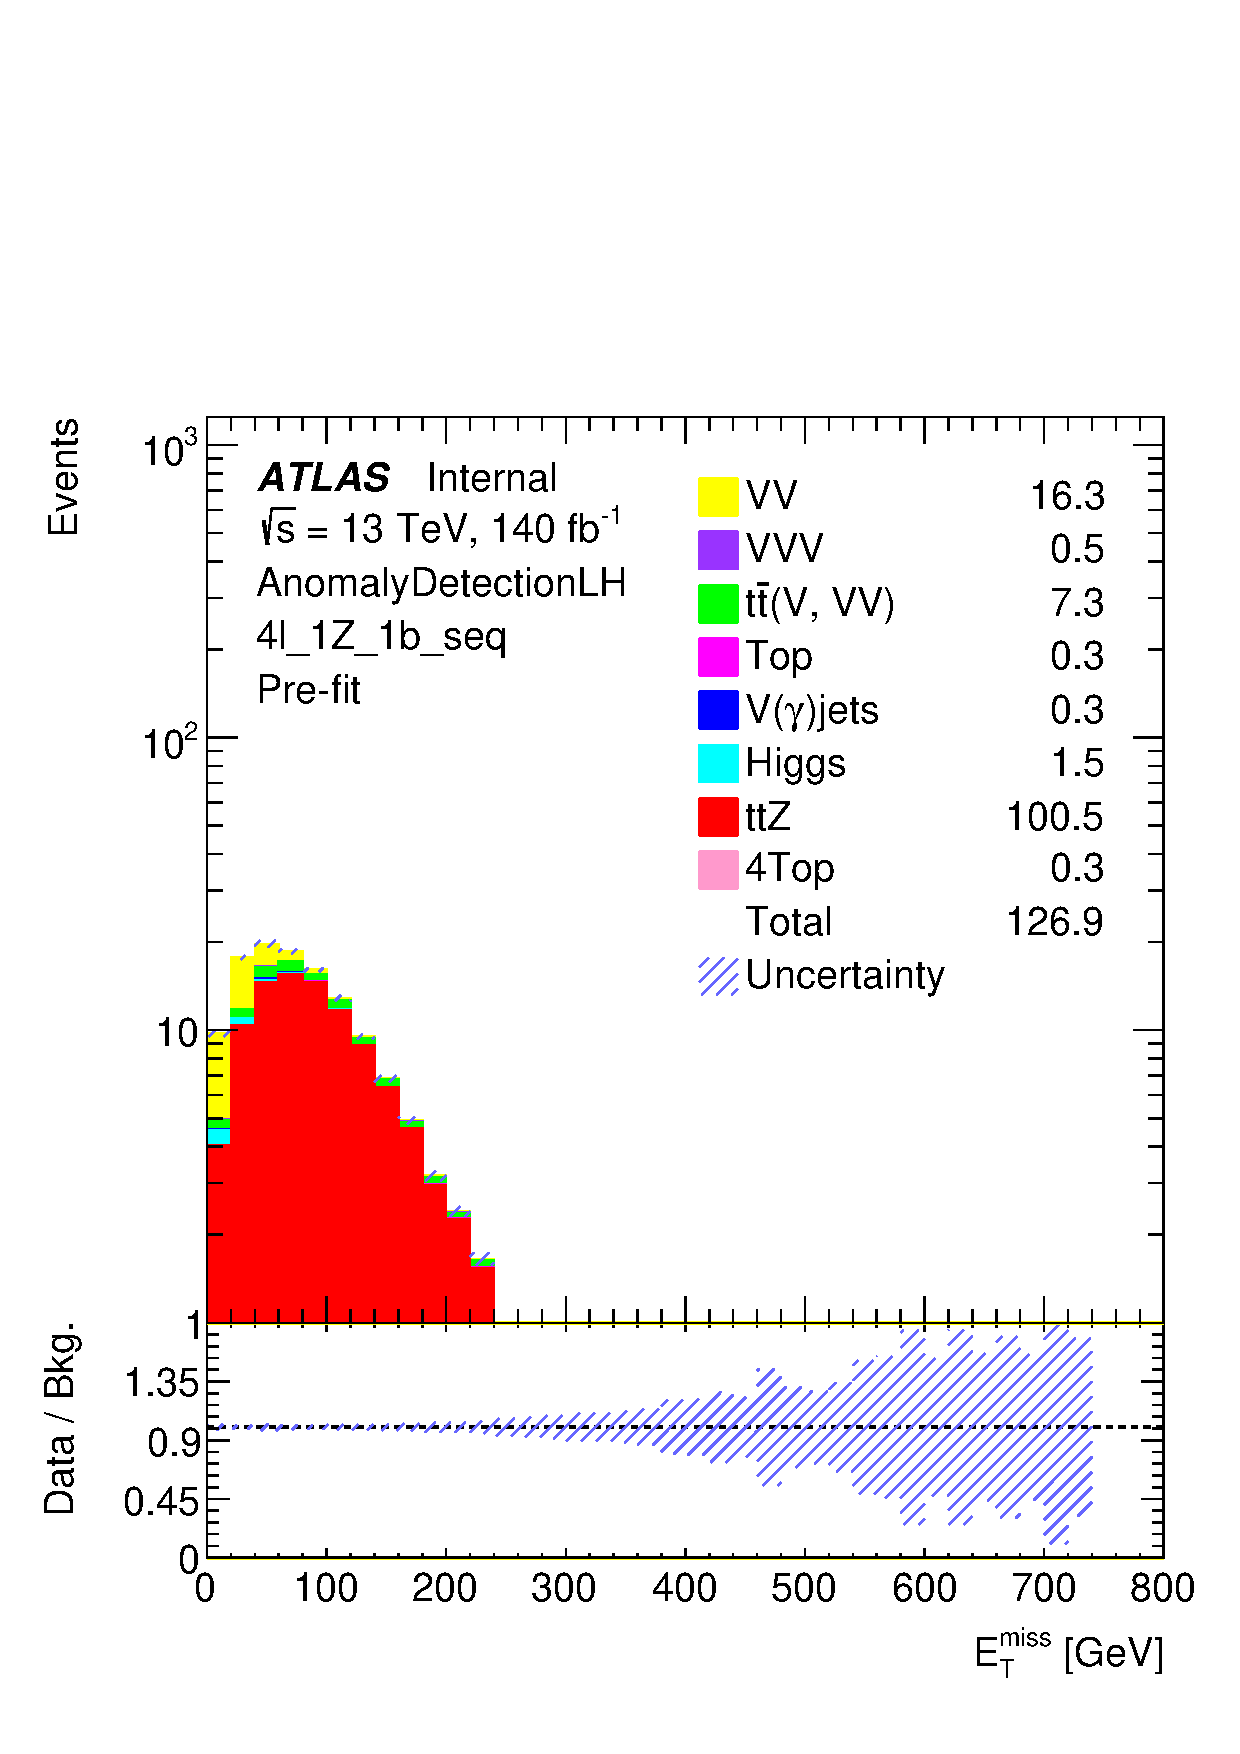
\includegraphics[width=0.24\textwidth]{plots/fourlepLH_run2/Plots/reg_4l_1Z_1b_seq_met.pdf} \\

\includegraphics[width=0.24\textwidth]{plots/fourlepLH_run2/Plots/reg_4l_1Z_1b_glob_m4l.pdf} &
\includegraphics[width=0.24\textwidth]{plots/fourlepLH_run2/Plots/reg_4l_1Z_1b_glob_HT_jets.pdf} &
\includegraphics[width=0.24\textwidth]{plots/fourlepLH_run2/Plots/reg_4l_1Z_1b_glob_HT_lep.pdf} &
\includegraphics[width=0.24\textwidth]{plots/fourlepLH_run2/Plots/reg_4l_1Z_1b_glob_met.pdf} \\

\end{tabular}
\end{frame}

\begin{frame}{\texttt{Results: 4l\_1Z\_1b}}
\begin{tabular}{cccccc}
\includegraphics[width=0.24\textwidth]{plots/fourlepLH_run2/Plots/reg_4l_1Z_1b_seq_nJets.pdf} &
\includegraphics[width=0.24\textwidth]{plots/fourlepLH_run2/Plots/reg_4l_1Z_1b_seq_nbJets.pdf} &
\includegraphics[width=0.24\textwidth]{plots/fourlepLH_run2/Plots/reg_4l_1Z_1b_seq_nElectrons.pdf} &
\includegraphics[width=0.24\textwidth]{plots/fourlepLH_run2/Plots/reg_4l_1Z_1b_seq_nMuons.pdf} \\

\includegraphics[width=0.24\textwidth]{plots/fourlepLH_run2/Plots/reg_4l_1Z_1b_glob_nJets.pdf} &
\includegraphics[width=0.24\textwidth]{plots/fourlepLH_run2/Plots/reg_4l_1Z_1b_glob_nbJets.pdf} &
\includegraphics[width=0.24\textwidth]{plots/fourlepLH_run2/Plots/reg_4l_1Z_1b_glob_nElectrons.pdf} &
\includegraphics[width=0.24\textwidth]{plots/fourlepLH_run2/Plots/reg_4l_1Z_1b_glob_nMuons.pdf} \\

\end{tabular}
\end{frame}

\begin{frame}{\texttt{Results: 4l\_1Z\_1b}}
\begin{tabular}{cccccc}
\includegraphics[width=0.24\textwidth]{plots/fourlepLH_run2/Plots/reg_4l_1Z_1b_seq_lep_pt_0.pdf} &
\includegraphics[width=0.24\textwidth]{plots/fourlepLH_run2/Plots/reg_4l_1Z_1b_seq_lep_pt_1.pdf} &
\includegraphics[width=0.24\textwidth]{plots/fourlepLH_run2/Plots/reg_4l_1Z_1b_seq_lep_pt_2.pdf} &
\includegraphics[width=0.24\textwidth]{plots/fourlepLH_run2/Plots/reg_4l_1Z_1b_seq_lep_pt_3.pdf} \\

\includegraphics[width=0.24\textwidth]{plots/fourlepLH_run2/Plots/reg_4l_1Z_1b_glob_lep_pt_0.pdf} &
\includegraphics[width=0.24\textwidth]{plots/fourlepLH_run2/Plots/reg_4l_1Z_1b_glob_lep_pt_1.pdf} &
\includegraphics[width=0.24\textwidth]{plots/fourlepLH_run2/Plots/reg_4l_1Z_1b_glob_lep_pt_2.pdf} &
\includegraphics[width=0.24\textwidth]{plots/fourlepLH_run2/Plots/reg_4l_1Z_1b_glob_lep_pt_3.pdf} \\

\end{tabular}

\end{frame}
\subsection{ZZ}
\begin{frame}{\texttt{Focused selection: ZZ}}
%\tiny
\centering
\begin{tabular}{|c|c|}
\hline

ZZ\_seq &
ZZ\_glob \\
\hline
\multicolumn{2}{|c|}{\texttt{globalTriggerMatchSLTorDLT\_LooseLH\_custTrig\_NOSYS}} \\
\multicolumn{2}{|c|}{\texttt{pass\_fourlep\_LooseLH\_NOSYS} }\\
\multicolumn{2}{|c|}{\texttt{$N_{leptons}$=4}} \\
\multicolumn{2}{|c|}{\texttt{$N_{taus}$ $= 0$} } \\
\multicolumn{2}{|c|}{$N_{b\mathrm{-jets}}$ $\geq 0$} \\
\multicolumn{2}{|c|}{\texttt{Q = 0}} \\

\hline

\texttt{$|m_{Z1}^{seq}-91.2e3| < 10e3$} &
\texttt{$|m_{Z1}^{glob}-91.2e3| < 10e3$} &\\
\texttt{$|m_{Z2}^{seq}-91.2e3| < 10e3$} &
\texttt{$|m_{Z2}^{glob}-91.2e3| < 10e3$}\\

\hline

\end{tabular}
\end{frame}

\begin{frame}{\texttt{Results: ZZ}}
\centering
\begin{tabular}{cccccc}

\includegraphics[width=0.24\textwidth]{plots/fourlepLH_run2/Plots/reg_ZZ_seq_Z1_mass_seq_1GeV.pdf} &
\includegraphics[width=0.24\textwidth]{plots/fourlepLH_run2/Plots/reg_ZZ_seq_Z2_mass_seq_1GeV.pdf}  &

\includegraphics[width=0.24\textwidth]{plots/fourlepLH_run2/Plots/reg_ZZ_glob_Z1_mass_glob_1GeV.pdf} &
\includegraphics[width=0.24\textwidth]{plots/fourlepLH_run2/Plots/reg_ZZ_glob_Z2_mass_glob_1GeV.pdf}\\

\includegraphics[width=0.24\textwidth]{plots/fourlepLH_run2/Plots/reg_ZZ_seq_Z1_pt_seq.pdf} &
\includegraphics[width=0.24\textwidth]{plots/fourlepLH_run2/Plots/reg_ZZ_seq_Z2_pt_seq.pdf}  &

\includegraphics[width=0.24\textwidth]{plots/fourlepLH_run2/Plots/reg_ZZ_glob_Z1_pt_glob.pdf} &
\includegraphics[width=0.24\textwidth]{plots/fourlepLH_run2/Plots/reg_ZZ_glob_Z2_pt_glob.pdf}
\end{tabular}
\end{frame}

\begin{frame}{\texttt{Results: ZZ}}
\begin{tabular}{cccccc}
\includegraphics[width=0.24\textwidth]{plots/fourlepLH_run2/Plots/reg_ZZ_seq_Zscore_seq.pdf} & 
\includegraphics[width=0.24\textwidth]{plots/fourlepLH_run2/Plots/reg_ZZ_seq_Zscore_glob.pdf}&
\includegraphics[width=0.24\textwidth]{plots/fourlepLH_run2/Plots/reg_ZZ_seq_deltaZscore.pdf}\\

\includegraphics[width=0.24\textwidth]{plots/fourlepLH_run2/Plots/reg_ZZ_glob_Zscore_seq.pdf} & 
\includegraphics[width=0.24\textwidth]{plots/fourlepLH_run2/Plots/reg_ZZ_glob_Zscore_glob.pdf}&
\includegraphics[width=0.24\textwidth]{plots/fourlepLH_run2/Plots/reg_ZZ_glob_deltaZscore.pdf}
\end{tabular}
\end{frame}


\begin{frame}{\texttt{Results: ZZ}}
\begin{tabular}{cccccc}

\includegraphics[width=0.24\textwidth]{plots/fourlepLH_run2/Plots/reg_ZZ_seq_m4l.pdf} &
\includegraphics[width=0.24\textwidth]{plots/fourlepLH_run2/Plots/reg_ZZ_seq_HT_jets.pdf} &
\includegraphics[width=0.24\textwidth]{plots/fourlepLH_run2/Plots/reg_ZZ_seq_HT_lep.pdf} &
\includegraphics[width=0.24\textwidth]{plots/fourlepLH_run2/Plots/reg_ZZ_seq_met.pdf} \\

\includegraphics[width=0.24\textwidth]{plots/fourlepLH_run2/Plots/reg_ZZ_glob_m4l.pdf} &
\includegraphics[width=0.24\textwidth]{plots/fourlepLH_run2/Plots/reg_ZZ_glob_HT_jets.pdf} &
\includegraphics[width=0.24\textwidth]{plots/fourlepLH_run2/Plots/reg_ZZ_glob_HT_lep.pdf} &
\includegraphics[width=0.24\textwidth]{plots/fourlepLH_run2/Plots/reg_ZZ_glob_met.pdf} \\

\end{tabular}
\end{frame}

\begin{frame}{\texttt{Results: ZZ}}
\begin{tabular}{cccccc}
\includegraphics[width=0.24\textwidth]{plots/fourlepLH_run2/Plots/reg_ZZ_seq_nJets.pdf} &
\includegraphics[width=0.24\textwidth]{plots/fourlepLH_run2/Plots/reg_ZZ_seq_nbJets.pdf} &
\includegraphics[width=0.24\textwidth]{plots/fourlepLH_run2/Plots/reg_ZZ_seq_nElectrons.pdf} &
\includegraphics[width=0.24\textwidth]{plots/fourlepLH_run2/Plots/reg_ZZ_seq_nMuons.pdf} \\

\includegraphics[width=0.24\textwidth]{plots/fourlepLH_run2/Plots/reg_ZZ_glob_nJets.pdf} &
\includegraphics[width=0.24\textwidth]{plots/fourlepLH_run2/Plots/reg_ZZ_glob_nbJets.pdf} &
\includegraphics[width=0.24\textwidth]{plots/fourlepLH_run2/Plots/reg_ZZ_glob_nElectrons.pdf} &
\includegraphics[width=0.24\textwidth]{plots/fourlepLH_run2/Plots/reg_ZZ_glob_nMuons.pdf} \\

\end{tabular}
\end{frame}

\begin{frame}{\texttt{Results: ZZ}}
\begin{tabular}{cccccc}
\includegraphics[width=0.24\textwidth]{plots/fourlepLH_run2/Plots/reg_ZZ_seq_lep_pt_0.pdf} &
\includegraphics[width=0.24\textwidth]{plots/fourlepLH_run2/Plots/reg_ZZ_seq_lep_pt_1.pdf} &
\includegraphics[width=0.24\textwidth]{plots/fourlepLH_run2/Plots/reg_ZZ_seq_lep_pt_2.pdf} &
\includegraphics[width=0.24\textwidth]{plots/fourlepLH_run2/Plots/reg_ZZ_seq_lep_pt_3.pdf} \\

\includegraphics[width=0.24\textwidth]{plots/fourlepLH_run2/Plots/reg_ZZ_glob_lep_pt_0.pdf} &
\includegraphics[width=0.24\textwidth]{plots/fourlepLH_run2/Plots/reg_ZZ_glob_lep_pt_1.pdf} &
\includegraphics[width=0.24\textwidth]{plots/fourlepLH_run2/Plots/reg_ZZ_glob_lep_pt_2.pdf} &
\includegraphics[width=0.24\textwidth]{plots/fourlepLH_run2/Plots/reg_ZZ_glob_lep_pt_3.pdf} \\

\end{tabular}

\end{frame}
\subsection{4l\_2Z\_0b}
\begin{frame}{\texttt{Focused selection: 4l\_2Z\_0b}}
%\tiny
\centering
\begin{tabular}{|c|c|}
\hline

4l\_2Z\_0b\_seq &
4l\_2Z\_0b\_glob \\
\hline
\multicolumn{2}{|c|}{\texttt{globalTriggerMatchSLTorDLT\_LooseLH\_custTrig\_NOSYS}} \\
\multicolumn{2}{|c|}{\texttt{pass\_fourlep\_LooseLH\_NOSYS} }\\
\multicolumn{2}{|c|}{\texttt{$N_{leptons}$=4}} \\
\multicolumn{2}{|c|}{\texttt{$N_{taus}$ $= 0$} } \\
\multicolumn{2}{|c|}{$N_{b\mathrm{-jets}}$ $= 0$} \\
\multicolumn{2}{|c|}{\texttt{Q = 0}} \\

\hline

\texttt{$|m_{Z1}^{seq}-91.2e3| < 10e3$} &
\texttt{$|m_{Z1}^{glob}-91.2e3| < 10e3$} &\\
\texttt{$|m_{Z2}^{seq}-91.2e3| < 10e3$} &
\texttt{$|m_{Z2}^{glob}-91.2e3| < 10e3$}\\

\hline

\end{tabular}
\end{frame}

\begin{frame}{\texttt{Results: 4l\_2Z\_0b}}
\centering
\begin{tabular}{cccccc}

\includegraphics[width=0.24\textwidth]{plots/fourlepLH_run2/Plots/reg_4l_2Z_0b_seq_Z1_mass_seq_1GeV.pdf} &
\includegraphics[width=0.24\textwidth]{plots/fourlepLH_run2/Plots/reg_4l_2Z_0b_seq_Z2_mass_seq_1GeV.pdf}  &

\includegraphics[width=0.24\textwidth]{plots/fourlepLH_run2/Plots/reg_4l_2Z_0b_glob_Z1_mass_glob_1GeV.pdf} &
\includegraphics[width=0.24\textwidth]{plots/fourlepLH_run2/Plots/reg_4l_2Z_0b_glob_Z2_mass_glob_1GeV.pdf}\\

\includegraphics[width=0.24\textwidth]{plots/fourlepLH_run2/Plots/reg_4l_2Z_0b_seq_Z1_pt_seq.pdf} &
\includegraphics[width=0.24\textwidth]{plots/fourlepLH_run2/Plots/reg_4l_2Z_0b_seq_Z2_pt_seq.pdf}  &

\includegraphics[width=0.24\textwidth]{plots/fourlepLH_run2/Plots/reg_4l_2Z_0b_glob_Z1_pt_glob.pdf} &
\includegraphics[width=0.24\textwidth]{plots/fourlepLH_run2/Plots/reg_4l_2Z_0b_glob_Z2_pt_glob.pdf}
\end{tabular}
\end{frame}

\begin{frame}{\texttt{Results: 4l\_2Z\_0b}}
\begin{tabular}{cccccc}
\includegraphics[width=0.24\textwidth]{plots/fourlepLH_run2/Plots/reg_4l_2Z_0b_seq_Zscore_seq.pdf} & 
\includegraphics[width=0.24\textwidth]{plots/fourlepLH_run2/Plots/reg_4l_2Z_0b_seq_Zscore_glob.pdf}&
\includegraphics[width=0.24\textwidth]{plots/fourlepLH_run2/Plots/reg_4l_2Z_0b_seq_deltaZscore.pdf}\\

\includegraphics[width=0.24\textwidth]{plots/fourlepLH_run2/Plots/reg_4l_2Z_0b_glob_Zscore_seq.pdf} & 
\includegraphics[width=0.24\textwidth]{plots/fourlepLH_run2/Plots/reg_4l_2Z_0b_glob_Zscore_glob.pdf}&
\includegraphics[width=0.24\textwidth]{plots/fourlepLH_run2/Plots/reg_4l_2Z_0b_glob_deltaZscore.pdf}
\end{tabular}
\end{frame}


\begin{frame}{\texttt{Results: 4l\_2Z\_0b}}
\begin{tabular}{cccccc}

\includegraphics[width=0.24\textwidth]{plots/fourlepLH_run2/Plots/reg_4l_2Z_0b_seq_m4l.pdf} &
\includegraphics[width=0.24\textwidth]{plots/fourlepLH_run2/Plots/reg_4l_2Z_0b_seq_HT_jets.pdf} &
\includegraphics[width=0.24\textwidth]{plots/fourlepLH_run2/Plots/reg_4l_2Z_0b_seq_HT_lep.pdf} &
\includegraphics[width=0.24\textwidth]{plots/fourlepLH_run2/Plots/reg_4l_2Z_0b_seq_met.pdf} \\

\includegraphics[width=0.24\textwidth]{plots/fourlepLH_run2/Plots/reg_4l_2Z_0b_glob_m4l.pdf} &
\includegraphics[width=0.24\textwidth]{plots/fourlepLH_run2/Plots/reg_4l_2Z_0b_glob_HT_jets.pdf} &
\includegraphics[width=0.24\textwidth]{plots/fourlepLH_run2/Plots/reg_4l_2Z_0b_glob_HT_lep.pdf} &
\includegraphics[width=0.24\textwidth]{plots/fourlepLH_run2/Plots/reg_4l_2Z_0b_glob_met.pdf} \\

\end{tabular}
\end{frame}

\begin{frame}{\texttt{Results: 4l\_2Z\_0b}}
\begin{tabular}{cccccc}
\includegraphics[width=0.24\textwidth]{plots/fourlepLH_run2/Plots/reg_4l_2Z_0b_seq_nJets.pdf} &
\includegraphics[width=0.24\textwidth]{plots/fourlepLH_run2/Plots/reg_4l_2Z_0b_seq_nbJets.pdf} &
\includegraphics[width=0.24\textwidth]{plots/fourlepLH_run2/Plots/reg_4l_2Z_0b_seq_nElectrons.pdf} &
\includegraphics[width=0.24\textwidth]{plots/fourlepLH_run2/Plots/reg_4l_2Z_0b_seq_nMuons.pdf} \\

\includegraphics[width=0.24\textwidth]{plots/fourlepLH_run2/Plots/reg_4l_2Z_0b_glob_nJets.pdf} &
\includegraphics[width=0.24\textwidth]{plots/fourlepLH_run2/Plots/reg_4l_2Z_0b_glob_nbJets.pdf} &
\includegraphics[width=0.24\textwidth]{plots/fourlepLH_run2/Plots/reg_4l_2Z_0b_glob_nElectrons.pdf} &
\includegraphics[width=0.24\textwidth]{plots/fourlepLH_run2/Plots/reg_4l_2Z_0b_glob_nMuons.pdf} \\

\end{tabular}
\end{frame}

\begin{frame}{\texttt{Results: 4l\_2Z\_0b}}
\begin{tabular}{cccccc}
\includegraphics[width=0.24\textwidth]{plots/fourlepLH_run2/Plots/reg_4l_2Z_0b_seq_lep_pt_0.pdf} &
\includegraphics[width=0.24\textwidth]{plots/fourlepLH_run2/Plots/reg_4l_2Z_0b_seq_lep_pt_1.pdf} &
\includegraphics[width=0.24\textwidth]{plots/fourlepLH_run2/Plots/reg_4l_2Z_0b_seq_lep_pt_2.pdf} &
\includegraphics[width=0.24\textwidth]{plots/fourlepLH_run2/Plots/reg_4l_2Z_0b_seq_lep_pt_3.pdf} \\

\includegraphics[width=0.24\textwidth]{plots/fourlepLH_run2/Plots/reg_4l_2Z_0b_glob_lep_pt_0.pdf} &
\includegraphics[width=0.24\textwidth]{plots/fourlepLH_run2/Plots/reg_4l_2Z_0b_glob_lep_pt_1.pdf} &
\includegraphics[width=0.24\textwidth]{plots/fourlepLH_run2/Plots/reg_4l_2Z_0b_glob_lep_pt_2.pdf} &
\includegraphics[width=0.24\textwidth]{plots/fourlepLH_run2/Plots/reg_4l_2Z_0b_glob_lep_pt_3.pdf} \\

\end{tabular}

\end{frame}
\subsection{4l\_2Z\_1b}
\begin{frame}{\texttt{Focused selection: 4l\_2Z\_1b}}
%\tiny
\centering
\begin{tabular}{|c|c|}
\hline

4l\_2Z\_1b\_seq &
4l\_2Z\_1b\_glob \\
\hline
\multicolumn{2}{|c|}{\texttt{globalTriggerMatchSLTorDLT\_LooseLH\_custTrig\_NOSYS}} \\
\multicolumn{2}{|c|}{\texttt{pass\_fourlep\_LooseLH\_NOSYS} }\\
\multicolumn{2}{|c|}{\texttt{$N_{leptons}$=4}} \\
\multicolumn{2}{|c|}{\texttt{$N_{taus}$ $= 0$} } \\
\multicolumn{2}{|c|}{$N_{b\mathrm{-jets}}$ $\geq 1$} \\
\multicolumn{2}{|c|}{\texttt{Q = 0}} \\

\hline

\texttt{$|m_{Z1}^{seq}-91.2e3| < 10e3$} &
\texttt{$|m_{Z1}^{glob}-91.2e3| < 10e3$} &\\
\texttt{$|m_{Z2}^{seq}-91.2e3| < 10e3$} &
\texttt{$|m_{Z2}^{glob}-91.2e3| < 10e3$}\\

\hline

\end{tabular}
\end{frame}

\begin{frame}{\texttt{Results: 4l\_2Z\_1b}}
\centering
\begin{tabular}{cccccc}

\includegraphics[width=0.24\textwidth]{plots/fourlepLH_run2/Plots/reg_4l_2Z_1b_seq_Z1_mass_seq_1GeV.pdf} &
\includegraphics[width=0.24\textwidth]{plots/fourlepLH_run2/Plots/reg_4l_2Z_1b_seq_Z2_mass_seq_1GeV.pdf}  &

\includegraphics[width=0.24\textwidth]{plots/fourlepLH_run2/Plots/reg_4l_2Z_1b_glob_Z1_mass_glob_1GeV.pdf} &
\includegraphics[width=0.24\textwidth]{plots/fourlepLH_run2/Plots/reg_4l_2Z_1b_glob_Z2_mass_glob_1GeV.pdf}\\

\includegraphics[width=0.24\textwidth]{plots/fourlepLH_run2/Plots/reg_4l_2Z_1b_seq_Z1_pt_seq.pdf} &
\includegraphics[width=0.24\textwidth]{plots/fourlepLH_run2/Plots/reg_4l_2Z_1b_seq_Z2_pt_seq.pdf}  &

\includegraphics[width=0.24\textwidth]{plots/fourlepLH_run2/Plots/reg_4l_2Z_1b_glob_Z1_pt_glob.pdf} &
\includegraphics[width=0.24\textwidth]{plots/fourlepLH_run2/Plots/reg_4l_2Z_1b_glob_Z2_pt_glob.pdf}
\end{tabular}
\end{frame}

\begin{frame}{\texttt{Results: 4l\_2Z\_1b}}
\begin{tabular}{cccccc}
\includegraphics[width=0.24\textwidth]{plots/fourlepLH_run2/Plots/reg_4l_2Z_1b_seq_Zscore_seq.pdf} & 
\includegraphics[width=0.24\textwidth]{plots/fourlepLH_run2/Plots/reg_4l_2Z_1b_seq_Zscore_glob.pdf}&
\includegraphics[width=0.24\textwidth]{plots/fourlepLH_run2/Plots/reg_4l_2Z_1b_seq_deltaZscore.pdf}\\

\includegraphics[width=0.24\textwidth]{plots/fourlepLH_run2/Plots/reg_4l_2Z_1b_glob_Zscore_seq.pdf} & 
\includegraphics[width=0.24\textwidth]{plots/fourlepLH_run2/Plots/reg_4l_2Z_1b_glob_Zscore_glob.pdf}&
\includegraphics[width=0.24\textwidth]{plots/fourlepLH_run2/Plots/reg_4l_2Z_1b_glob_deltaZscore.pdf}
\end{tabular}
\end{frame}


\begin{frame}{\texttt{Results: 4l\_2Z\_1b}}
\begin{tabular}{cccccc}

\includegraphics[width=0.24\textwidth]{plots/fourlepLH_run2/Plots/reg_4l_2Z_1b_seq_m4l.pdf} &
\includegraphics[width=0.24\textwidth]{plots/fourlepLH_run2/Plots/reg_4l_2Z_1b_seq_HT_jets.pdf} &
\includegraphics[width=0.24\textwidth]{plots/fourlepLH_run2/Plots/reg_4l_2Z_1b_seq_HT_lep.pdf} &
\includegraphics[width=0.24\textwidth]{plots/fourlepLH_run2/Plots/reg_4l_2Z_1b_seq_met.pdf} \\

\includegraphics[width=0.24\textwidth]{plots/fourlepLH_run2/Plots/reg_4l_2Z_1b_glob_m4l.pdf} &
\includegraphics[width=0.24\textwidth]{plots/fourlepLH_run2/Plots/reg_4l_2Z_1b_glob_HT_jets.pdf} &
\includegraphics[width=0.24\textwidth]{plots/fourlepLH_run2/Plots/reg_4l_2Z_1b_glob_HT_lep.pdf} &
\includegraphics[width=0.24\textwidth]{plots/fourlepLH_run2/Plots/reg_4l_2Z_1b_glob_met.pdf} \\

\end{tabular}
\end{frame}

\begin{frame}{\texttt{Results: 4l\_2Z\_1b}}
\begin{tabular}{cccccc}
\includegraphics[width=0.24\textwidth]{plots/fourlepLH_run2/Plots/reg_4l_2Z_1b_seq_nJets.pdf} &
\includegraphics[width=0.24\textwidth]{plots/fourlepLH_run2/Plots/reg_4l_2Z_1b_seq_nbJets.pdf} &
\includegraphics[width=0.24\textwidth]{plots/fourlepLH_run2/Plots/reg_4l_2Z_1b_seq_nElectrons.pdf} &
\includegraphics[width=0.24\textwidth]{plots/fourlepLH_run2/Plots/reg_4l_2Z_1b_seq_nMuons.pdf} \\

\includegraphics[width=0.24\textwidth]{plots/fourlepLH_run2/Plots/reg_4l_2Z_1b_glob_nJets.pdf} &
\includegraphics[width=0.24\textwidth]{plots/fourlepLH_run2/Plots/reg_4l_2Z_1b_glob_nbJets.pdf} &
\includegraphics[width=0.24\textwidth]{plots/fourlepLH_run2/Plots/reg_4l_2Z_1b_glob_nElectrons.pdf} &
\includegraphics[width=0.24\textwidth]{plots/fourlepLH_run2/Plots/reg_4l_2Z_1b_glob_nMuons.pdf} \\

\end{tabular}
\end{frame}

\begin{frame}{\texttt{Results: 4l\_2Z\_1b}}
\begin{tabular}{cccccc}
\includegraphics[width=0.24\textwidth]{plots/fourlepLH_run2/Plots/reg_4l_2Z_1b_seq_lep_pt_0.pdf} &
\includegraphics[width=0.24\textwidth]{plots/fourlepLH_run2/Plots/reg_4l_2Z_1b_seq_lep_pt_1.pdf} &
\includegraphics[width=0.24\textwidth]{plots/fourlepLH_run2/Plots/reg_4l_2Z_1b_seq_lep_pt_2.pdf} &
\includegraphics[width=0.24\textwidth]{plots/fourlepLH_run2/Plots/reg_4l_2Z_1b_seq_lep_pt_3.pdf} \\

\includegraphics[width=0.24\textwidth]{plots/fourlepLH_run2/Plots/reg_4l_2Z_1b_glob_lep_pt_0.pdf} &
\includegraphics[width=0.24\textwidth]{plots/fourlepLH_run2/Plots/reg_4l_2Z_1b_glob_lep_pt_1.pdf} &
\includegraphics[width=0.24\textwidth]{plots/fourlepLH_run2/Plots/reg_4l_2Z_1b_glob_lep_pt_2.pdf} &
\includegraphics[width=0.24\textwidth]{plots/fourlepLH_run2/Plots/reg_4l_2Z_1b_glob_lep_pt_3.pdf} \\

\end{tabular}

\end{frame}
\subsection{4l\_2Q}
\begin{frame}{\texttt{Focused selection: 4l\_2Q}}
%\tiny
\centering
\begin{tabular}{|c|c|}
\hline

4l\_2Q\_seq &
4l\_2Q\_glob \\
\hline
\multicolumn{2}{|c|}{\texttt{globalTriggerMatchSLTorDLT\_LooseLH\_custTrig\_NOSYS}} \\
\multicolumn{2}{|c|}{\texttt{pass\_fourlep\_LooseLH\_NOSYS} }\\
\multicolumn{2}{|c|}{\texttt{$N_{leptons}$=4}} \\
\multicolumn{2}{|c|}{\texttt{$N_{taus}$ $\geq 0$} } \\
\multicolumn{2}{|c|}{$N_{b\mathrm{-jets}}$ $\geq 0$} \\
\multicolumn{2}{|c|}{\texttt{Q = 2}} \\

\hline

\texttt{$|m_{Z1}^{seq}-91.2e3| < 10e3$} &
\texttt{$|m_{Z1}^{glob}-91.2e3| < 10e3$} &\\
\texttt{$|m_{Z2}^{seq}-91.2e3| < 10e3$} &
\texttt{$|m_{Z2}^{glob}-91.2e3| < 10e3$}\\

\hline

\end{tabular}
\end{frame}

\begin{frame}{\texttt{Results: 4l\_2Q}}
\centering
\begin{tabular}{cccccc}

\includegraphics[width=0.24\textwidth]{plots/fourlepLH_run2/Plots/reg_4l_2Q_seq_Z1_mass_seq_1GeV.pdf} &
\includegraphics[width=0.24\textwidth]{plots/fourlepLH_run2/Plots/reg_4l_2Q_seq_Z2_mass_seq_1GeV.pdf}  &

\includegraphics[width=0.24\textwidth]{plots/fourlepLH_run2/Plots/reg_4l_2Q_glob_Z1_mass_glob_1GeV.pdf} &
\includegraphics[width=0.24\textwidth]{plots/fourlepLH_run2/Plots/reg_4l_2Q_glob_Z2_mass_glob_1GeV.pdf}\\

\includegraphics[width=0.24\textwidth]{plots/fourlepLH_run2/Plots/reg_4l_2Q_seq_Z1_pt_seq.pdf} &
\includegraphics[width=0.24\textwidth]{plots/fourlepLH_run2/Plots/reg_4l_2Q_seq_Z2_pt_seq.pdf}  &

\includegraphics[width=0.24\textwidth]{plots/fourlepLH_run2/Plots/reg_4l_2Q_glob_Z1_pt_glob.pdf} &
\includegraphics[width=0.24\textwidth]{plots/fourlepLH_run2/Plots/reg_4l_2Q_glob_Z2_pt_glob.pdf}
\end{tabular}
\end{frame}

\begin{frame}{\texttt{Results: 4l\_2Q}}
\begin{tabular}{cccccc}
\includegraphics[width=0.24\textwidth]{plots/fourlepLH_run2/Plots/reg_4l_2Q_seq_Zscore_seq.pdf} & 
\includegraphics[width=0.24\textwidth]{plots/fourlepLH_run2/Plots/reg_4l_2Q_seq_Zscore_glob.pdf}&
\includegraphics[width=0.24\textwidth]{plots/fourlepLH_run2/Plots/reg_4l_2Q_seq_deltaZscore.pdf}\\

\includegraphics[width=0.24\textwidth]{plots/fourlepLH_run2/Plots/reg_4l_2Q_glob_Zscore_seq.pdf} & 
\includegraphics[width=0.24\textwidth]{plots/fourlepLH_run2/Plots/reg_4l_2Q_glob_Zscore_glob.pdf}&
\includegraphics[width=0.24\textwidth]{plots/fourlepLH_run2/Plots/reg_4l_2Q_glob_deltaZscore.pdf}
\end{tabular}
\end{frame}


\begin{frame}{\texttt{Results: 4l\_2Q}}
\begin{tabular}{cccccc}

\includegraphics[width=0.24\textwidth]{plots/fourlepLH_run2/Plots/reg_4l_2Q_seq_m4l.pdf} &
\includegraphics[width=0.24\textwidth]{plots/fourlepLH_run2/Plots/reg_4l_2Q_seq_HT_jets.pdf} &
\includegraphics[width=0.24\textwidth]{plots/fourlepLH_run2/Plots/reg_4l_2Q_seq_HT_lep.pdf} &
\includegraphics[width=0.24\textwidth]{plots/fourlepLH_run2/Plots/reg_4l_2Q_seq_met.pdf} \\

\includegraphics[width=0.24\textwidth]{plots/fourlepLH_run2/Plots/reg_4l_2Q_glob_m4l.pdf} &
\includegraphics[width=0.24\textwidth]{plots/fourlepLH_run2/Plots/reg_4l_2Q_glob_HT_jets.pdf} &
\includegraphics[width=0.24\textwidth]{plots/fourlepLH_run2/Plots/reg_4l_2Q_glob_HT_lep.pdf} &
\includegraphics[width=0.24\textwidth]{plots/fourlepLH_run2/Plots/reg_4l_2Q_glob_met.pdf} \\

\end{tabular}
\end{frame}

\begin{frame}{\texttt{Results: 4l\_2Q}}
\begin{tabular}{cccccc}
\includegraphics[width=0.24\textwidth]{plots/fourlepLH_run2/Plots/reg_4l_2Q_seq_nJets.pdf} &
\includegraphics[width=0.24\textwidth]{plots/fourlepLH_run2/Plots/reg_4l_2Q_seq_nbJets.pdf} &
\includegraphics[width=0.24\textwidth]{plots/fourlepLH_run2/Plots/reg_4l_2Q_seq_nElectrons.pdf} &
\includegraphics[width=0.24\textwidth]{plots/fourlepLH_run2/Plots/reg_4l_2Q_seq_nMuons.pdf} \\

\includegraphics[width=0.24\textwidth]{plots/fourlepLH_run2/Plots/reg_4l_2Q_glob_nJets.pdf} &
\includegraphics[width=0.24\textwidth]{plots/fourlepLH_run2/Plots/reg_4l_2Q_glob_nbJets.pdf} &
\includegraphics[width=0.24\textwidth]{plots/fourlepLH_run2/Plots/reg_4l_2Q_glob_nElectrons.pdf} &
\includegraphics[width=0.24\textwidth]{plots/fourlepLH_run2/Plots/reg_4l_2Q_glob_nMuons.pdf} \\

\end{tabular}
\end{frame}

\begin{frame}{\texttt{Results: 4l\_2Q}}
\begin{tabular}{cccccc}
\includegraphics[width=0.24\textwidth]{plots/fourlepLH_run2/Plots/reg_4l_2Q_seq_lep_pt_0.pdf} &
\includegraphics[width=0.24\textwidth]{plots/fourlepLH_run2/Plots/reg_4l_2Q_seq_lep_pt_1.pdf} &
\includegraphics[width=0.24\textwidth]{plots/fourlepLH_run2/Plots/reg_4l_2Q_seq_lep_pt_2.pdf} &
\includegraphics[width=0.24\textwidth]{plots/fourlepLH_run2/Plots/reg_4l_2Q_seq_lep_pt_3.pdf} \\

\includegraphics[width=0.24\textwidth]{plots/fourlepLH_run2/Plots/reg_4l_2Q_glob_lep_pt_0.pdf} &
\includegraphics[width=0.24\textwidth]{plots/fourlepLH_run2/Plots/reg_4l_2Q_glob_lep_pt_1.pdf} &
\includegraphics[width=0.24\textwidth]{plots/fourlepLH_run2/Plots/reg_4l_2Q_glob_lep_pt_2.pdf} &
\includegraphics[width=0.24\textwidth]{plots/fourlepLH_run2/Plots/reg_4l_2Q_glob_lep_pt_3.pdf} \\

\end{tabular}

\end{frame}
\subsection{4l\_2Q\_0Z\_0b}
\begin{frame}{\texttt{Focused selection: 4l\_2Q\_0Z\_0b}}
%\tiny
\centering
\begin{tabular}{|c|c|}
\hline

4l\_2Q\_0Z\_0b\_seq &
4l\_2Q\_0Z\_0b\_glob \\
\hline
\multicolumn{2}{|c|}{\texttt{globalTriggerMatchSLTorDLT\_LooseLH\_custTrig\_NOSYS}} \\
\multicolumn{2}{|c|}{\texttt{pass\_fourlep\_LooseLH\_NOSYS} }\\
\multicolumn{2}{|c|}{\texttt{$N_{leptons}$=4}} \\
\multicolumn{2}{|c|}{\texttt{$N_{taus}$ $\geq 0$} } \\
\multicolumn{2}{|c|}{$N_{b\mathrm{-jets}}$ $= 0$} \\
\multicolumn{2}{|c|}{\texttt{Q = 2}} \\

\hline

\texttt{$|m_{Z1}^{seq}-91.2e3| < 10e3$} &
\texttt{$|m_{Z1}^{glob}-91.2e3| < 10e3$} &\\
\texttt{$|m_{Z2}^{seq}-91.2e3| < 10e3$} &
\texttt{$|m_{Z2}^{glob}-91.2e3| < 10e3$}\\

\hline

\end{tabular}
\end{frame}

\begin{frame}{\texttt{Results: 4l\_2Q\_0Z\_0b}}
\centering
\begin{tabular}{cccccc}

\includegraphics[width=0.24\textwidth]{plots/fourlepLH_run2/Plots/reg_4l_2Q_0Z_0b_seq_Z1_mass_seq_1GeV.pdf} &
\includegraphics[width=0.24\textwidth]{plots/fourlepLH_run2/Plots/reg_4l_2Q_0Z_0b_seq_Z2_mass_seq_1GeV.pdf}  &

\includegraphics[width=0.24\textwidth]{plots/fourlepLH_run2/Plots/reg_4l_2Q_0Z_0b_glob_Z1_mass_glob_1GeV.pdf} &
\includegraphics[width=0.24\textwidth]{plots/fourlepLH_run2/Plots/reg_4l_2Q_0Z_0b_glob_Z2_mass_glob_1GeV.pdf}\\

\includegraphics[width=0.24\textwidth]{plots/fourlepLH_run2/Plots/reg_4l_2Q_0Z_0b_seq_Z1_pt_seq.pdf} &
\includegraphics[width=0.24\textwidth]{plots/fourlepLH_run2/Plots/reg_4l_2Q_0Z_0b_seq_Z2_pt_seq.pdf}  &

\includegraphics[width=0.24\textwidth]{plots/fourlepLH_run2/Plots/reg_4l_2Q_0Z_0b_glob_Z1_pt_glob.pdf} &
\includegraphics[width=0.24\textwidth]{plots/fourlepLH_run2/Plots/reg_4l_2Q_0Z_0b_glob_Z2_pt_glob.pdf}
\end{tabular}
\end{frame}

\begin{frame}{\texttt{Results: 4l\_2Q\_0Z\_0b}}
\begin{tabular}{cccccc}
\includegraphics[width=0.24\textwidth]{plots/fourlepLH_run2/Plots/reg_4l_2Q_0Z_0b_seq_Zscore_seq.pdf} & 
\includegraphics[width=0.24\textwidth]{plots/fourlepLH_run2/Plots/reg_4l_2Q_0Z_0b_seq_Zscore_glob.pdf}&
\includegraphics[width=0.24\textwidth]{plots/fourlepLH_run2/Plots/reg_4l_2Q_0Z_0b_seq_deltaZscore.pdf}\\

\includegraphics[width=0.24\textwidth]{plots/fourlepLH_run2/Plots/reg_4l_2Q_0Z_0b_glob_Zscore_seq.pdf} & 
\includegraphics[width=0.24\textwidth]{plots/fourlepLH_run2/Plots/reg_4l_2Q_0Z_0b_glob_Zscore_glob.pdf}&
\includegraphics[width=0.24\textwidth]{plots/fourlepLH_run2/Plots/reg_4l_2Q_0Z_0b_glob_deltaZscore.pdf}
\end{tabular}
\end{frame}


\begin{frame}{\texttt{Results: 4l\_2Q\_0Z\_0b}}
\begin{tabular}{cccccc}

\includegraphics[width=0.24\textwidth]{plots/fourlepLH_run2/Plots/reg_4l_2Q_0Z_0b_seq_m4l.pdf} &
\includegraphics[width=0.24\textwidth]{plots/fourlepLH_run2/Plots/reg_4l_2Q_0Z_0b_seq_HT_jets.pdf} &
\includegraphics[width=0.24\textwidth]{plots/fourlepLH_run2/Plots/reg_4l_2Q_0Z_0b_seq_HT_lep.pdf} &
\includegraphics[width=0.24\textwidth]{plots/fourlepLH_run2/Plots/reg_4l_2Q_0Z_0b_seq_met.pdf} \\

\includegraphics[width=0.24\textwidth]{plots/fourlepLH_run2/Plots/reg_4l_2Q_0Z_0b_glob_m4l.pdf} &
\includegraphics[width=0.24\textwidth]{plots/fourlepLH_run2/Plots/reg_4l_2Q_0Z_0b_glob_HT_jets.pdf} &
\includegraphics[width=0.24\textwidth]{plots/fourlepLH_run2/Plots/reg_4l_2Q_0Z_0b_glob_HT_lep.pdf} &
\includegraphics[width=0.24\textwidth]{plots/fourlepLH_run2/Plots/reg_4l_2Q_0Z_0b_glob_met.pdf} \\

\end{tabular}
\end{frame}

\begin{frame}{\texttt{Results: 4l\_2Q\_0Z\_0b}}
\begin{tabular}{cccccc}
\includegraphics[width=0.24\textwidth]{plots/fourlepLH_run2/Plots/reg_4l_2Q_0Z_0b_seq_nJets.pdf} &
\includegraphics[width=0.24\textwidth]{plots/fourlepLH_run2/Plots/reg_4l_2Q_0Z_0b_seq_nbJets.pdf} &
\includegraphics[width=0.24\textwidth]{plots/fourlepLH_run2/Plots/reg_4l_2Q_0Z_0b_seq_nElectrons.pdf} &
\includegraphics[width=0.24\textwidth]{plots/fourlepLH_run2/Plots/reg_4l_2Q_0Z_0b_seq_nMuons.pdf} \\

\includegraphics[width=0.24\textwidth]{plots/fourlepLH_run2/Plots/reg_4l_2Q_0Z_0b_glob_nJets.pdf} &
\includegraphics[width=0.24\textwidth]{plots/fourlepLH_run2/Plots/reg_4l_2Q_0Z_0b_glob_nbJets.pdf} &
\includegraphics[width=0.24\textwidth]{plots/fourlepLH_run2/Plots/reg_4l_2Q_0Z_0b_glob_nElectrons.pdf} &
\includegraphics[width=0.24\textwidth]{plots/fourlepLH_run2/Plots/reg_4l_2Q_0Z_0b_glob_nMuons.pdf} \\

\end{tabular}
\end{frame}

\begin{frame}{\texttt{Results: 4l\_2Q\_0Z\_0b}}
\begin{tabular}{cccccc}
\includegraphics[width=0.24\textwidth]{plots/fourlepLH_run2/Plots/reg_4l_2Q_0Z_0b_seq_lep_pt_0.pdf} &
\includegraphics[width=0.24\textwidth]{plots/fourlepLH_run2/Plots/reg_4l_2Q_0Z_0b_seq_lep_pt_1.pdf} &
\includegraphics[width=0.24\textwidth]{plots/fourlepLH_run2/Plots/reg_4l_2Q_0Z_0b_seq_lep_pt_2.pdf} &
\includegraphics[width=0.24\textwidth]{plots/fourlepLH_run2/Plots/reg_4l_2Q_0Z_0b_seq_lep_pt_3.pdf} \\

\includegraphics[width=0.24\textwidth]{plots/fourlepLH_run2/Plots/reg_4l_2Q_0Z_0b_glob_lep_pt_0.pdf} &
\includegraphics[width=0.24\textwidth]{plots/fourlepLH_run2/Plots/reg_4l_2Q_0Z_0b_glob_lep_pt_1.pdf} &
\includegraphics[width=0.24\textwidth]{plots/fourlepLH_run2/Plots/reg_4l_2Q_0Z_0b_glob_lep_pt_2.pdf} &
\includegraphics[width=0.24\textwidth]{plots/fourlepLH_run2/Plots/reg_4l_2Q_0Z_0b_glob_lep_pt_3.pdf} \\

\end{tabular}

\end{frame}
\subsection{4l\_2Q\_0Z\_1b}
\begin{frame}{\texttt{Focused selection: 4l\_2Q\_0Z\_1b}}
%\tiny
\centering
\begin{tabular}{|c|c|}
\hline

4l\_2Q\_0Z\_1b\_seq &
4l\_2Q\_0Z\_1b\_glob \\
\hline
\multicolumn{2}{|c|}{\texttt{globalTriggerMatchSLTorDLT\_LooseLH\_custTrig\_NOSYS}} \\
\multicolumn{2}{|c|}{\texttt{pass\_fourlep\_LooseLH\_NOSYS} }\\
\multicolumn{2}{|c|}{\texttt{$N_{leptons}$=4}} \\
\multicolumn{2}{|c|}{\texttt{$N_{taus}$ $\geq 0$} } \\
\multicolumn{2}{|c|}{$N_{b\mathrm{-jets}}$ $\geq 1$} \\
\multicolumn{2}{|c|}{\texttt{Q = 2}} \\

\hline

\texttt{$|m_{Z1}^{seq}-91.2e3| < 10e3$} &
\texttt{$|m_{Z1}^{glob}-91.2e3| < 10e3$} &\\
\texttt{$|m_{Z2}^{seq}-91.2e3| < 10e3$} &
\texttt{$|m_{Z2}^{glob}-91.2e3| < 10e3$}\\

\hline

\end{tabular}
\end{frame}

\begin{frame}{\texttt{Results: 4l\_2Q\_0Z\_1b}}
\centering
\begin{tabular}{cccccc}

\includegraphics[width=0.24\textwidth]{plots/fourlepLH_run2/Plots/reg_4l_2Q_0Z_1b_seq_Z1_mass_seq_1GeV.pdf} &
\includegraphics[width=0.24\textwidth]{plots/fourlepLH_run2/Plots/reg_4l_2Q_0Z_1b_seq_Z2_mass_seq_1GeV.pdf}  &

\includegraphics[width=0.24\textwidth]{plots/fourlepLH_run2/Plots/reg_4l_2Q_0Z_1b_glob_Z1_mass_glob_1GeV.pdf} &
\includegraphics[width=0.24\textwidth]{plots/fourlepLH_run2/Plots/reg_4l_2Q_0Z_1b_glob_Z2_mass_glob_1GeV.pdf}\\

\includegraphics[width=0.24\textwidth]{plots/fourlepLH_run2/Plots/reg_4l_2Q_0Z_1b_seq_Z1_pt_seq.pdf} &
\includegraphics[width=0.24\textwidth]{plots/fourlepLH_run2/Plots/reg_4l_2Q_0Z_1b_seq_Z2_pt_seq.pdf}  &

\includegraphics[width=0.24\textwidth]{plots/fourlepLH_run2/Plots/reg_4l_2Q_0Z_1b_glob_Z1_pt_glob.pdf} &
\includegraphics[width=0.24\textwidth]{plots/fourlepLH_run2/Plots/reg_4l_2Q_0Z_1b_glob_Z2_pt_glob.pdf}
\end{tabular}
\end{frame}

\begin{frame}{\texttt{Results: 4l\_2Q\_0Z\_1b}}
\begin{tabular}{cccccc}
\includegraphics[width=0.24\textwidth]{plots/fourlepLH_run2/Plots/reg_4l_2Q_0Z_1b_seq_Zscore_seq.pdf} & 
\includegraphics[width=0.24\textwidth]{plots/fourlepLH_run2/Plots/reg_4l_2Q_0Z_1b_seq_Zscore_glob.pdf}&
\includegraphics[width=0.24\textwidth]{plots/fourlepLH_run2/Plots/reg_4l_2Q_0Z_1b_seq_deltaZscore.pdf}\\

\includegraphics[width=0.24\textwidth]{plots/fourlepLH_run2/Plots/reg_4l_2Q_0Z_1b_glob_Zscore_seq.pdf} & 
\includegraphics[width=0.24\textwidth]{plots/fourlepLH_run2/Plots/reg_4l_2Q_0Z_1b_glob_Zscore_glob.pdf}&
\includegraphics[width=0.24\textwidth]{plots/fourlepLH_run2/Plots/reg_4l_2Q_0Z_1b_glob_deltaZscore.pdf}
\end{tabular}
\end{frame}


\begin{frame}{\texttt{Results: 4l\_2Q\_0Z\_1b}}
\begin{tabular}{cccccc}

\includegraphics[width=0.24\textwidth]{plots/fourlepLH_run2/Plots/reg_4l_2Q_0Z_1b_seq_m4l.pdf} &
\includegraphics[width=0.24\textwidth]{plots/fourlepLH_run2/Plots/reg_4l_2Q_0Z_1b_seq_HT_jets.pdf} &
\includegraphics[width=0.24\textwidth]{plots/fourlepLH_run2/Plots/reg_4l_2Q_0Z_1b_seq_HT_lep.pdf} &
\includegraphics[width=0.24\textwidth]{plots/fourlepLH_run2/Plots/reg_4l_2Q_0Z_1b_seq_met.pdf} \\

\includegraphics[width=0.24\textwidth]{plots/fourlepLH_run2/Plots/reg_4l_2Q_0Z_1b_glob_m4l.pdf} &
\includegraphics[width=0.24\textwidth]{plots/fourlepLH_run2/Plots/reg_4l_2Q_0Z_1b_glob_HT_jets.pdf} &
\includegraphics[width=0.24\textwidth]{plots/fourlepLH_run2/Plots/reg_4l_2Q_0Z_1b_glob_HT_lep.pdf} &
\includegraphics[width=0.24\textwidth]{plots/fourlepLH_run2/Plots/reg_4l_2Q_0Z_1b_glob_met.pdf} \\

\end{tabular}
\end{frame}

\begin{frame}{\texttt{Results: 4l\_2Q\_0Z\_1b}}
\begin{tabular}{cccccc}
\includegraphics[width=0.24\textwidth]{plots/fourlepLH_run2/Plots/reg_4l_2Q_0Z_1b_seq_nJets.pdf} &
\includegraphics[width=0.24\textwidth]{plots/fourlepLH_run2/Plots/reg_4l_2Q_0Z_1b_seq_nbJets.pdf} &
\includegraphics[width=0.24\textwidth]{plots/fourlepLH_run2/Plots/reg_4l_2Q_0Z_1b_seq_nElectrons.pdf} &
\includegraphics[width=0.24\textwidth]{plots/fourlepLH_run2/Plots/reg_4l_2Q_0Z_1b_seq_nMuons.pdf} \\

\includegraphics[width=0.24\textwidth]{plots/fourlepLH_run2/Plots/reg_4l_2Q_0Z_1b_glob_nJets.pdf} &
\includegraphics[width=0.24\textwidth]{plots/fourlepLH_run2/Plots/reg_4l_2Q_0Z_1b_glob_nbJets.pdf} &
\includegraphics[width=0.24\textwidth]{plots/fourlepLH_run2/Plots/reg_4l_2Q_0Z_1b_glob_nElectrons.pdf} &
\includegraphics[width=0.24\textwidth]{plots/fourlepLH_run2/Plots/reg_4l_2Q_0Z_1b_glob_nMuons.pdf} \\

\end{tabular}
\end{frame}

\begin{frame}{\texttt{Results: 4l\_2Q\_0Z\_1b}}
\begin{tabular}{cccccc}
\includegraphics[width=0.24\textwidth]{plots/fourlepLH_run2/Plots/reg_4l_2Q_0Z_1b_seq_lep_pt_0.pdf} &
\includegraphics[width=0.24\textwidth]{plots/fourlepLH_run2/Plots/reg_4l_2Q_0Z_1b_seq_lep_pt_1.pdf} &
\includegraphics[width=0.24\textwidth]{plots/fourlepLH_run2/Plots/reg_4l_2Q_0Z_1b_seq_lep_pt_2.pdf} &
\includegraphics[width=0.24\textwidth]{plots/fourlepLH_run2/Plots/reg_4l_2Q_0Z_1b_seq_lep_pt_3.pdf} \\

\includegraphics[width=0.24\textwidth]{plots/fourlepLH_run2/Plots/reg_4l_2Q_0Z_1b_glob_lep_pt_0.pdf} &
\includegraphics[width=0.24\textwidth]{plots/fourlepLH_run2/Plots/reg_4l_2Q_0Z_1b_glob_lep_pt_1.pdf} &
\includegraphics[width=0.24\textwidth]{plots/fourlepLH_run2/Plots/reg_4l_2Q_0Z_1b_glob_lep_pt_2.pdf} &
\includegraphics[width=0.24\textwidth]{plots/fourlepLH_run2/Plots/reg_4l_2Q_0Z_1b_glob_lep_pt_3.pdf} \\

\end{tabular}

\end{frame}
\subsection{4l\_2Q\_1Z\_0b}
\begin{frame}{\texttt{Focused selection: 4l\_2Q\_1Z\_0b}}
%\tiny
\centering
\begin{tabular}{|c|c|}
\hline

4l\_2Q\_1Z\_0b\_seq &
4l\_2Q\_1Z\_0b\_glob \\
\hline
\multicolumn{2}{|c|}{\texttt{globalTriggerMatchSLTorDLT\_LooseLH\_custTrig\_NOSYS}} \\
\multicolumn{2}{|c|}{\texttt{pass\_fourlep\_LooseLH\_NOSYS} }\\
\multicolumn{2}{|c|}{\texttt{$N_{leptons}$=4}} \\
\multicolumn{2}{|c|}{\texttt{$N_{taus}$ $\geq 0$} } \\
\multicolumn{2}{|c|}{$N_{b\mathrm{-jets}}$ $= 0$} \\
\multicolumn{2}{|c|}{\texttt{Q = 2}} \\

\hline

\texttt{$|m_{Z1}^{seq}-91.2e3| < 10e3$} &
\texttt{$|m_{Z1}^{glob}-91.2e3| < 10e3$} &\\
\texttt{$|m_{Z2}^{seq}-91.2e3| < 10e3$} &
\texttt{$|m_{Z2}^{glob}-91.2e3| < 10e3$}\\

\hline

\end{tabular}
\end{frame}

\begin{frame}{\texttt{Results: 4l\_2Q\_1Z\_0b}}
\centering
\begin{tabular}{cccccc}

\includegraphics[width=0.24\textwidth]{plots/fourlepLH_run2/Plots/reg_4l_2Q_1Z_0b_seq_Z1_mass_seq_1GeV.pdf} &
\includegraphics[width=0.24\textwidth]{plots/fourlepLH_run2/Plots/reg_4l_2Q_1Z_0b_seq_Z2_mass_seq_1GeV.pdf}  &

\includegraphics[width=0.24\textwidth]{plots/fourlepLH_run2/Plots/reg_4l_2Q_1Z_0b_glob_Z1_mass_glob_1GeV.pdf} &
\includegraphics[width=0.24\textwidth]{plots/fourlepLH_run2/Plots/reg_4l_2Q_1Z_0b_glob_Z2_mass_glob_1GeV.pdf}\\

\includegraphics[width=0.24\textwidth]{plots/fourlepLH_run2/Plots/reg_4l_2Q_1Z_0b_seq_Z1_pt_seq.pdf} &
\includegraphics[width=0.24\textwidth]{plots/fourlepLH_run2/Plots/reg_4l_2Q_1Z_0b_seq_Z2_pt_seq.pdf}  &

\includegraphics[width=0.24\textwidth]{plots/fourlepLH_run2/Plots/reg_4l_2Q_1Z_0b_glob_Z1_pt_glob.pdf} &
\includegraphics[width=0.24\textwidth]{plots/fourlepLH_run2/Plots/reg_4l_2Q_1Z_0b_glob_Z2_pt_glob.pdf}
\end{tabular}
\end{frame}

\begin{frame}{\texttt{Results: 4l\_2Q\_1Z\_0b}}
\begin{tabular}{cccccc}
\includegraphics[width=0.24\textwidth]{plots/fourlepLH_run2/Plots/reg_4l_2Q_1Z_0b_seq_Zscore_seq.pdf} & 
\includegraphics[width=0.24\textwidth]{plots/fourlepLH_run2/Plots/reg_4l_2Q_1Z_0b_seq_Zscore_glob.pdf}&
\includegraphics[width=0.24\textwidth]{plots/fourlepLH_run2/Plots/reg_4l_2Q_1Z_0b_seq_deltaZscore.pdf}\\

\includegraphics[width=0.24\textwidth]{plots/fourlepLH_run2/Plots/reg_4l_2Q_1Z_0b_glob_Zscore_seq.pdf} & 
\includegraphics[width=0.24\textwidth]{plots/fourlepLH_run2/Plots/reg_4l_2Q_1Z_0b_glob_Zscore_glob.pdf}&
\includegraphics[width=0.24\textwidth]{plots/fourlepLH_run2/Plots/reg_4l_2Q_1Z_0b_glob_deltaZscore.pdf}
\end{tabular}
\end{frame}


\begin{frame}{\texttt{Results: 4l\_2Q\_1Z\_0b}}
\begin{tabular}{cccccc}

\includegraphics[width=0.24\textwidth]{plots/fourlepLH_run2/Plots/reg_4l_2Q_1Z_0b_seq_m4l.pdf} &
\includegraphics[width=0.24\textwidth]{plots/fourlepLH_run2/Plots/reg_4l_2Q_1Z_0b_seq_HT_jets.pdf} &
\includegraphics[width=0.24\textwidth]{plots/fourlepLH_run2/Plots/reg_4l_2Q_1Z_0b_seq_HT_lep.pdf} &
\includegraphics[width=0.24\textwidth]{plots/fourlepLH_run2/Plots/reg_4l_2Q_1Z_0b_seq_met.pdf} \\

\includegraphics[width=0.24\textwidth]{plots/fourlepLH_run2/Plots/reg_4l_2Q_1Z_0b_glob_m4l.pdf} &
\includegraphics[width=0.24\textwidth]{plots/fourlepLH_run2/Plots/reg_4l_2Q_1Z_0b_glob_HT_jets.pdf} &
\includegraphics[width=0.24\textwidth]{plots/fourlepLH_run2/Plots/reg_4l_2Q_1Z_0b_glob_HT_lep.pdf} &
\includegraphics[width=0.24\textwidth]{plots/fourlepLH_run2/Plots/reg_4l_2Q_1Z_0b_glob_met.pdf} \\

\end{tabular}
\end{frame}

\begin{frame}{\texttt{Results: 4l\_2Q\_1Z\_0b}}
\begin{tabular}{cccccc}
\includegraphics[width=0.24\textwidth]{plots/fourlepLH_run2/Plots/reg_4l_2Q_1Z_0b_seq_nJets.pdf} &
\includegraphics[width=0.24\textwidth]{plots/fourlepLH_run2/Plots/reg_4l_2Q_1Z_0b_seq_nbJets.pdf} &
\includegraphics[width=0.24\textwidth]{plots/fourlepLH_run2/Plots/reg_4l_2Q_1Z_0b_seq_nElectrons.pdf} &
\includegraphics[width=0.24\textwidth]{plots/fourlepLH_run2/Plots/reg_4l_2Q_1Z_0b_seq_nMuons.pdf} \\

\includegraphics[width=0.24\textwidth]{plots/fourlepLH_run2/Plots/reg_4l_2Q_1Z_0b_glob_nJets.pdf} &
\includegraphics[width=0.24\textwidth]{plots/fourlepLH_run2/Plots/reg_4l_2Q_1Z_0b_glob_nbJets.pdf} &
\includegraphics[width=0.24\textwidth]{plots/fourlepLH_run2/Plots/reg_4l_2Q_1Z_0b_glob_nElectrons.pdf} &
\includegraphics[width=0.24\textwidth]{plots/fourlepLH_run2/Plots/reg_4l_2Q_1Z_0b_glob_nMuons.pdf} \\

\end{tabular}
\end{frame}

\begin{frame}{\texttt{Results: 4l\_2Q\_1Z\_0b}}
\begin{tabular}{cccccc}
\includegraphics[width=0.24\textwidth]{plots/fourlepLH_run2/Plots/reg_4l_2Q_1Z_0b_seq_lep_pt_0.pdf} &
\includegraphics[width=0.24\textwidth]{plots/fourlepLH_run2/Plots/reg_4l_2Q_1Z_0b_seq_lep_pt_1.pdf} &
\includegraphics[width=0.24\textwidth]{plots/fourlepLH_run2/Plots/reg_4l_2Q_1Z_0b_seq_lep_pt_2.pdf} &
\includegraphics[width=0.24\textwidth]{plots/fourlepLH_run2/Plots/reg_4l_2Q_1Z_0b_seq_lep_pt_3.pdf} \\

\includegraphics[width=0.24\textwidth]{plots/fourlepLH_run2/Plots/reg_4l_2Q_1Z_0b_glob_lep_pt_0.pdf} &
\includegraphics[width=0.24\textwidth]{plots/fourlepLH_run2/Plots/reg_4l_2Q_1Z_0b_glob_lep_pt_1.pdf} &
\includegraphics[width=0.24\textwidth]{plots/fourlepLH_run2/Plots/reg_4l_2Q_1Z_0b_glob_lep_pt_2.pdf} &
\includegraphics[width=0.24\textwidth]{plots/fourlepLH_run2/Plots/reg_4l_2Q_1Z_0b_glob_lep_pt_3.pdf} \\

\end{tabular}

\end{frame}
\subsection{4l\_2Q\_1Z\_1b}
\begin{frame}{\texttt{Focused selection: 4l\_2Q\_1Z\_1b}}
%\tiny
\centering
\begin{tabular}{|c|c|}
\hline

4l\_2Q\_1Z\_1b\_seq &
4l\_2Q\_1Z\_1b\_glob \\
\hline
\multicolumn{2}{|c|}{\texttt{globalTriggerMatchSLTorDLT\_LooseLH\_custTrig\_NOSYS}} \\
\multicolumn{2}{|c|}{\texttt{pass\_fourlep\_LooseLH\_NOSYS} }\\
\multicolumn{2}{|c|}{\texttt{$N_{leptons}$=4}} \\
\multicolumn{2}{|c|}{\texttt{$N_{taus}$ $\geq 0$} } \\
\multicolumn{2}{|c|}{$N_{b\mathrm{-jets}}$ $\geq 1$} \\
\multicolumn{2}{|c|}{\texttt{Q = 2}} \\

\hline

\texttt{$|m_{Z1}^{seq}-91.2e3| < 10e3$} &
\texttt{$|m_{Z1}^{glob}-91.2e3| < 10e3$} &\\
\texttt{$|m_{Z2}^{seq}-91.2e3| < 10e3$} &
\texttt{$|m_{Z2}^{glob}-91.2e3| < 10e3$}\\

\hline

\end{tabular}
\end{frame}

\begin{frame}{\texttt{Results: 4l\_2Q\_1Z\_1b}}
\centering
\begin{tabular}{cccccc}

\includegraphics[width=0.24\textwidth]{plots/fourlepLH_run2/Plots/reg_4l_2Q_1Z_1b_seq_Z1_mass_seq_1GeV.pdf} &
\includegraphics[width=0.24\textwidth]{plots/fourlepLH_run2/Plots/reg_4l_2Q_1Z_1b_seq_Z2_mass_seq_1GeV.pdf}  &

\includegraphics[width=0.24\textwidth]{plots/fourlepLH_run2/Plots/reg_4l_2Q_1Z_1b_glob_Z1_mass_glob_1GeV.pdf} &
\includegraphics[width=0.24\textwidth]{plots/fourlepLH_run2/Plots/reg_4l_2Q_1Z_1b_glob_Z2_mass_glob_1GeV.pdf}\\

\includegraphics[width=0.24\textwidth]{plots/fourlepLH_run2/Plots/reg_4l_2Q_1Z_1b_seq_Z1_pt_seq.pdf} &
\includegraphics[width=0.24\textwidth]{plots/fourlepLH_run2/Plots/reg_4l_2Q_1Z_1b_seq_Z2_pt_seq.pdf}  &

\includegraphics[width=0.24\textwidth]{plots/fourlepLH_run2/Plots/reg_4l_2Q_1Z_1b_glob_Z1_pt_glob.pdf} &
\includegraphics[width=0.24\textwidth]{plots/fourlepLH_run2/Plots/reg_4l_2Q_1Z_1b_glob_Z2_pt_glob.pdf}
\end{tabular}
\end{frame}

\begin{frame}{\texttt{Results: 4l\_2Q\_1Z\_1b}}
\begin{tabular}{cccccc}
\includegraphics[width=0.24\textwidth]{plots/fourlepLH_run2/Plots/reg_4l_2Q_1Z_1b_seq_Zscore_seq.pdf} & 
\includegraphics[width=0.24\textwidth]{plots/fourlepLH_run2/Plots/reg_4l_2Q_1Z_1b_seq_Zscore_glob.pdf}&
\includegraphics[width=0.24\textwidth]{plots/fourlepLH_run2/Plots/reg_4l_2Q_1Z_1b_seq_deltaZscore.pdf}\\

\includegraphics[width=0.24\textwidth]{plots/fourlepLH_run2/Plots/reg_4l_2Q_1Z_1b_glob_Zscore_seq.pdf} & 
\includegraphics[width=0.24\textwidth]{plots/fourlepLH_run2/Plots/reg_4l_2Q_1Z_1b_glob_Zscore_glob.pdf}&
\includegraphics[width=0.24\textwidth]{plots/fourlepLH_run2/Plots/reg_4l_2Q_1Z_1b_glob_deltaZscore.pdf}
\end{tabular}
\end{frame}


\begin{frame}{\texttt{Results: 4l\_2Q\_1Z\_1b}}
\begin{tabular}{cccccc}

\includegraphics[width=0.24\textwidth]{plots/fourlepLH_run2/Plots/reg_4l_2Q_1Z_1b_seq_m4l.pdf} &
\includegraphics[width=0.24\textwidth]{plots/fourlepLH_run2/Plots/reg_4l_2Q_1Z_1b_seq_HT_jets.pdf} &
\includegraphics[width=0.24\textwidth]{plots/fourlepLH_run2/Plots/reg_4l_2Q_1Z_1b_seq_HT_lep.pdf} &
\includegraphics[width=0.24\textwidth]{plots/fourlepLH_run2/Plots/reg_4l_2Q_1Z_1b_seq_met.pdf} \\

\includegraphics[width=0.24\textwidth]{plots/fourlepLH_run2/Plots/reg_4l_2Q_1Z_1b_glob_m4l.pdf} &
\includegraphics[width=0.24\textwidth]{plots/fourlepLH_run2/Plots/reg_4l_2Q_1Z_1b_glob_HT_jets.pdf} &
\includegraphics[width=0.24\textwidth]{plots/fourlepLH_run2/Plots/reg_4l_2Q_1Z_1b_glob_HT_lep.pdf} &
\includegraphics[width=0.24\textwidth]{plots/fourlepLH_run2/Plots/reg_4l_2Q_1Z_1b_glob_met.pdf} \\

\end{tabular}
\end{frame}

\begin{frame}{\texttt{Results: 4l\_2Q\_1Z\_1b}}
\begin{tabular}{cccccc}
\includegraphics[width=0.24\textwidth]{plots/fourlepLH_run2/Plots/reg_4l_2Q_1Z_1b_seq_nJets.pdf} &
\includegraphics[width=0.24\textwidth]{plots/fourlepLH_run2/Plots/reg_4l_2Q_1Z_1b_seq_nbJets.pdf} &
\includegraphics[width=0.24\textwidth]{plots/fourlepLH_run2/Plots/reg_4l_2Q_1Z_1b_seq_nElectrons.pdf} &
\includegraphics[width=0.24\textwidth]{plots/fourlepLH_run2/Plots/reg_4l_2Q_1Z_1b_seq_nMuons.pdf} \\

\includegraphics[width=0.24\textwidth]{plots/fourlepLH_run2/Plots/reg_4l_2Q_1Z_1b_glob_nJets.pdf} &
\includegraphics[width=0.24\textwidth]{plots/fourlepLH_run2/Plots/reg_4l_2Q_1Z_1b_glob_nbJets.pdf} &
\includegraphics[width=0.24\textwidth]{plots/fourlepLH_run2/Plots/reg_4l_2Q_1Z_1b_glob_nElectrons.pdf} &
\includegraphics[width=0.24\textwidth]{plots/fourlepLH_run2/Plots/reg_4l_2Q_1Z_1b_glob_nMuons.pdf} \\

\end{tabular}
\end{frame}

\begin{frame}{\texttt{Results: 4l\_2Q\_1Z\_1b}}
\begin{tabular}{cccccc}
\includegraphics[width=0.24\textwidth]{plots/fourlepLH_run2/Plots/reg_4l_2Q_1Z_1b_seq_lep_pt_0.pdf} &
\includegraphics[width=0.24\textwidth]{plots/fourlepLH_run2/Plots/reg_4l_2Q_1Z_1b_seq_lep_pt_1.pdf} &
\includegraphics[width=0.24\textwidth]{plots/fourlepLH_run2/Plots/reg_4l_2Q_1Z_1b_seq_lep_pt_2.pdf} &
\includegraphics[width=0.24\textwidth]{plots/fourlepLH_run2/Plots/reg_4l_2Q_1Z_1b_seq_lep_pt_3.pdf} \\

\includegraphics[width=0.24\textwidth]{plots/fourlepLH_run2/Plots/reg_4l_2Q_1Z_1b_glob_lep_pt_0.pdf} &
\includegraphics[width=0.24\textwidth]{plots/fourlepLH_run2/Plots/reg_4l_2Q_1Z_1b_glob_lep_pt_1.pdf} &
\includegraphics[width=0.24\textwidth]{plots/fourlepLH_run2/Plots/reg_4l_2Q_1Z_1b_glob_lep_pt_2.pdf} &
\includegraphics[width=0.24\textwidth]{plots/fourlepLH_run2/Plots/reg_4l_2Q_1Z_1b_glob_lep_pt_3.pdf} \\

\end{tabular}

\end{frame}
\subsection{4l\_4Q}
\begin{frame}{\texttt{Focused selection: 4l\_4Q}}
%\tiny
\centering
\begin{tabular}{|c|c|}
\hline

4l\_4Q\_seq &
4l\_4Q\_glob \\
\hline
\multicolumn{2}{|c|}{\texttt{globalTriggerMatchSLTorDLT\_LooseLH\_custTrig\_NOSYS}} \\
\multicolumn{2}{|c|}{\texttt{pass\_fourlep\_LooseLH\_NOSYS} }\\
\multicolumn{2}{|c|}{\texttt{$N_{leptons}$=4}} \\
\multicolumn{2}{|c|}{\texttt{$N_{taus}$ $\geq 0$} } \\
\multicolumn{2}{|c|}{$N_{b\mathrm{-jets}}$ $\geq 0$} \\
\multicolumn{2}{|c|}{\texttt{Q = 4}} \\

\hline

\texttt{$|m_{Z1}^{seq}-91.2e3| < 10e3$} &
\texttt{$|m_{Z1}^{glob}-91.2e3| < 10e3$} &\\
\texttt{$|m_{Z2}^{seq}-91.2e3| < 10e3$} &
\texttt{$|m_{Z2}^{glob}-91.2e3| < 10e3$}\\

\hline

\end{tabular}
\end{frame}

\begin{frame}{\texttt{Results: 4l\_4Q}}
\centering
\begin{tabular}{cccccc}

\includegraphics[width=0.24\textwidth]{plots/fourlepLH_run2/Plots/reg_4l_4Q_seq_Z1_mass_seq_1GeV.pdf} &
\includegraphics[width=0.24\textwidth]{plots/fourlepLH_run2/Plots/reg_4l_4Q_seq_Z2_mass_seq_1GeV.pdf}  &

\includegraphics[width=0.24\textwidth]{plots/fourlepLH_run2/Plots/reg_4l_4Q_glob_Z1_mass_glob_1GeV.pdf} &
\includegraphics[width=0.24\textwidth]{plots/fourlepLH_run2/Plots/reg_4l_4Q_glob_Z2_mass_glob_1GeV.pdf}\\

\includegraphics[width=0.24\textwidth]{plots/fourlepLH_run2/Plots/reg_4l_4Q_seq_Z1_pt_seq.pdf} &
\includegraphics[width=0.24\textwidth]{plots/fourlepLH_run2/Plots/reg_4l_4Q_seq_Z2_pt_seq.pdf}  &

\includegraphics[width=0.24\textwidth]{plots/fourlepLH_run2/Plots/reg_4l_4Q_glob_Z1_pt_glob.pdf} &
\includegraphics[width=0.24\textwidth]{plots/fourlepLH_run2/Plots/reg_4l_4Q_glob_Z2_pt_glob.pdf}
\end{tabular}
\end{frame}

\begin{frame}{\texttt{Results: 4l\_4Q}}
\begin{tabular}{cccccc}
\includegraphics[width=0.24\textwidth]{plots/fourlepLH_run2/Plots/reg_4l_4Q_seq_Zscore_seq.pdf} & 
\includegraphics[width=0.24\textwidth]{plots/fourlepLH_run2/Plots/reg_4l_4Q_seq_Zscore_glob.pdf}&
\includegraphics[width=0.24\textwidth]{plots/fourlepLH_run2/Plots/reg_4l_4Q_seq_deltaZscore.pdf}\\

\includegraphics[width=0.24\textwidth]{plots/fourlepLH_run2/Plots/reg_4l_4Q_glob_Zscore_seq.pdf} & 
\includegraphics[width=0.24\textwidth]{plots/fourlepLH_run2/Plots/reg_4l_4Q_glob_Zscore_glob.pdf}&
\includegraphics[width=0.24\textwidth]{plots/fourlepLH_run2/Plots/reg_4l_4Q_glob_deltaZscore.pdf}
\end{tabular}
\end{frame}


\begin{frame}{\texttt{Results: 4l\_4Q}}
\begin{tabular}{cccccc}

\includegraphics[width=0.24\textwidth]{plots/fourlepLH_run2/Plots/reg_4l_4Q_seq_m4l.pdf} &
\includegraphics[width=0.24\textwidth]{plots/fourlepLH_run2/Plots/reg_4l_4Q_seq_HT_jets.pdf} &
\includegraphics[width=0.24\textwidth]{plots/fourlepLH_run2/Plots/reg_4l_4Q_seq_HT_lep.pdf} &
\includegraphics[width=0.24\textwidth]{plots/fourlepLH_run2/Plots/reg_4l_4Q_seq_met.pdf} \\

\includegraphics[width=0.24\textwidth]{plots/fourlepLH_run2/Plots/reg_4l_4Q_glob_m4l.pdf} &
\includegraphics[width=0.24\textwidth]{plots/fourlepLH_run2/Plots/reg_4l_4Q_glob_HT_jets.pdf} &
\includegraphics[width=0.24\textwidth]{plots/fourlepLH_run2/Plots/reg_4l_4Q_glob_HT_lep.pdf} &
\includegraphics[width=0.24\textwidth]{plots/fourlepLH_run2/Plots/reg_4l_4Q_glob_met.pdf} \\

\end{tabular}
\end{frame}

\begin{frame}{\texttt{Results: 4l\_4Q}}
\begin{tabular}{cccccc}
\includegraphics[width=0.24\textwidth]{plots/fourlepLH_run2/Plots/reg_4l_4Q_seq_nJets.pdf} &
\includegraphics[width=0.24\textwidth]{plots/fourlepLH_run2/Plots/reg_4l_4Q_seq_nbJets.pdf} &
\includegraphics[width=0.24\textwidth]{plots/fourlepLH_run2/Plots/reg_4l_4Q_seq_nElectrons.pdf} &
\includegraphics[width=0.24\textwidth]{plots/fourlepLH_run2/Plots/reg_4l_4Q_seq_nMuons.pdf} \\

\includegraphics[width=0.24\textwidth]{plots/fourlepLH_run2/Plots/reg_4l_4Q_glob_nJets.pdf} &
\includegraphics[width=0.24\textwidth]{plots/fourlepLH_run2/Plots/reg_4l_4Q_glob_nbJets.pdf} &
\includegraphics[width=0.24\textwidth]{plots/fourlepLH_run2/Plots/reg_4l_4Q_glob_nElectrons.pdf} &
\includegraphics[width=0.24\textwidth]{plots/fourlepLH_run2/Plots/reg_4l_4Q_glob_nMuons.pdf} \\

\end{tabular}
\end{frame}

\begin{frame}{\texttt{Results: 4l\_4Q}}
\begin{tabular}{cccccc}
\includegraphics[width=0.24\textwidth]{plots/fourlepLH_run2/Plots/reg_4l_4Q_seq_lep_pt_0.pdf} &
\includegraphics[width=0.24\textwidth]{plots/fourlepLH_run2/Plots/reg_4l_4Q_seq_lep_pt_1.pdf} &
\includegraphics[width=0.24\textwidth]{plots/fourlepLH_run2/Plots/reg_4l_4Q_seq_lep_pt_2.pdf} &
\includegraphics[width=0.24\textwidth]{plots/fourlepLH_run2/Plots/reg_4l_4Q_seq_lep_pt_3.pdf} \\

\includegraphics[width=0.24\textwidth]{plots/fourlepLH_run2/Plots/reg_4l_4Q_glob_lep_pt_0.pdf} &
\includegraphics[width=0.24\textwidth]{plots/fourlepLH_run2/Plots/reg_4l_4Q_glob_lep_pt_1.pdf} &
\includegraphics[width=0.24\textwidth]{plots/fourlepLH_run2/Plots/reg_4l_4Q_glob_lep_pt_2.pdf} &
\includegraphics[width=0.24\textwidth]{plots/fourlepLH_run2/Plots/reg_4l_4Q_glob_lep_pt_3.pdf} \\

\end{tabular}

\end{frame}


\section{\texttt{Run3 LH}}
\include{slides_LH_run3}


\end{document}
